\documentclass[a4paper,11pt]{report}
\usepackage[utf8]{inputenc}
\usepackage[T1]{fontenc}
\usepackage[francais]{babel}
\usepackage{amsmath}
\usepackage{geometry}
\usepackage[pdftex]{graphicx}
\usepackage[font={small,it}]{caption}
\usepackage{subfigure}
\subfigcapmargin = .5cm
\usepackage{subcaption}
\usepackage{textcomp}
\usepackage[svgnames]{xcolor}
\usepackage{tikz}
\usetikzlibrary{mindmap}
\usepackage{pstricks}
\usepackage[section]{placeins}
\usepackage{amssymb}
\usepackage{cancel}
\usepackage{braket}
\usepackage{cite}
\usepackage{etex}
% \reserveinserts{28}
\usepackage{morefloats}
\usepackage{rotating}
\usepackage{cases}
%\usepackage{comment}
%\usepackage{fancyhdr}
\usepackage[toc,page]{appendix}
%\usepackage[page]{appendix}
\usepackage{pdflscape}
\usepackage{multicol}
\usepackage{comment}
\usepackage{stmaryrd}

\usepackage{hyperref} % Créer des liens et des signets 
\hypersetup{
  colorlinks=true, %colorise les liens 
  breaklinks=true, %permet le retour à la ligne dans les liens trop longs 
  urlcolor= blue, %couleur des hyperliens 
  linkcolor= DarkSlateGrey,	%couleur des liens internes 
  citecolor= DarkSlateGrey,	%couleur des références 
  pdftitle={M\'emoire de th\`ese}, %informations apparaissant dans 
  pdfauthor={Lo\"ic Cousin}, %les informations du document 
  pdfsubject={Trajectom\'etrie dans le cadre du projet europ\'een AIDA}
  bookmark=true
  linktocpage=true
}

\title{Trajectom\'etrie dans le cadre du projet europ\'een AIDA}
\author{Lo\"ic COUSIN}
\date{\today}

\begin{document}

\maketitle

\pdfbookmark{\contentsname}{toc}
\tableofcontents
\cleardoublepage
\pdfbookmark{Table de figures}{lof}
\listoffigures

\addtocontents{toc}{\protect\pagenumbering{roman}}  % pour la table des matières
\addtocontents{lof}{\protect\pagenumbering{roman}}  % pour la table des figures


\setcounter{secnumdepth}{2}

% \pagestyle{fancy}

\cleardoublepage

\pagenumbering{arabic}
\setcounter{page}{1}

% \cleardoublepage
\newpage
%\null
%\newpage

\pdfbookmark{Introduction}{Introduction}
\chapter*{Introduction}

Depuis les ann\'ees 70, le Mod\`ele Standard est le fer de lance th\'eorique de la physique des particules. Il permet un accord avec les r\'esultats exp\'erimentaux allant jusqu'au pour mille. Une seule pierre angulaire \`a l'\'edifice \'etait manquante : le secteur de Brout-Englert-Higgs. Le m\'ecanisme de Higgs permet de briser spontan\'ement la sym\'etrie \'electrofaible et g\'en\`ere la masse des particules \'el\'ementaires. Postul\'ee th\'eoriquement depuis l'ann\'ee 1964, c'est le 4 Juillet 2012, au CERN, que la d\'ecouverte exp\'erimentale du boson de Higgs par les exp\'eriences du LHC, ATLAS et CMS, a \'et\'e proclam\'ee. Cette d\'ecouverte a \'et\'e r\'ealis\'ee avec une \'energie dans le centre de masse de 7 et 8 $TeV$. Ce grand succ\`es, permis par le Large Hadron Collider (LHC), a ouvert la voie \`a l'\'etude du boson de Higgs et de ses propri\'et\'es.

\medskip

En d\'epit de son grand succ\`es, le Mod\`ele Standard ne permet pas de d\'ecrire tous les ph\'enom\`enes physiques observ\'es dans la nature. Par exemple, il ne d\'ecrit ni la gravitation ni la mati\`ere noire. Après une interruption de presque deux ans, le LHC va red\'emarrer en 2015. Son programme de recherche continuera avec cette fois-ci une \'energie dans le centre de masse de 13-14 $TeV$. Les donn\'ees recueillies permettront de mieux connaître les propri\'et\'es du boson de Higgs et de rechercher des manifestations de physique au-delà du mod\`ele standard. Cependant, d'autres acc\'el\'erateurs de particules visant \`a \'eclaircir ces questions sont \`a l'\'etude. Ils permettront de r\'epondre, conjointement avec le LHC, aux deux grandes questions de la physique des particules d'aujourd'hui : la brisure spontan\'ee de la sym\'etrie \'electrofaible et la recherche d'une nouvelle physique. L'International Linear Collider (ILC) fait partie de ces projets d'acc\'el\'erateurs. Il devrait voir le jour \`a l'horizon 2030. Il s'agit d'un collisionneur lin\'eaire d'\'electrons et de positons. Les collisions $e^- \, e^+$ permettent une plus grande pr\'ecision de mesure que les collisionneurs hadroniques comme le LHC. En effet, l'\'etat initial est parfaitement connu et le bruit de fond QCD est quasi-inexistant. L'ILC permettra une \'etude fine de la masse, de la largeur, des couplages et des nombres quantiques du boson de Higgs. En particulier, les diff\'erents processus de production du boson de Higgs (Higgsstrahlung, fusion $WW$, fusion $ZZ$) permettront de mesurer ces grandeurs. De plus, gr\^ace notamment aux mesures de grandes pr\'ecisions qu'il permettra, l'ILC ouvrira la voie \`a la d\'ecouverte d'une physique nouvelle.

% , $t\overline{t}H$
\medskip

L'une des \'etudes r\'ealisables \`a l'ILC concernera les couplages du boson de Higgs aux fermions et aux bosons de jauge (voire \`a lui-m\^eme). Une pr\'ecision allant de l'ordre de quelques pour-cents \`a quelques pour-milles devrait \^etre atteinte. Ces \'etudes requièrent un excellent \'etiquetage des saveurs lourdes. Le d\'efi r\'eside dans l'\'etiquetage pr\'ecis des jets issus des quarks $c$ et des leptons $\tau$. Cette t\^ache est rendue difficile par la faible distance de vol de ces particules, de l'ordre de 100 $\mu m$. Afin de distinguer ces saveurs, un d\'etecteur de vertex adapt\'e est n\'ecessaire. Il devra \^etre conçu \`a partir de capteurs atteignant une r\'esolution spatiale de l'ordre de quelques microm\`etres. De plus il devra pr\'esenter un budget de mati\`ere r\'eduit, avoir sa premi\`ere couche la plus proche possible du point d'interaction et devra enfin avoir un temps de lecture adapt\'e au taux d'occupation domin\'e par le bruit de fond du faisceau, provenent essentiellement du processus de \textit{beamstrahlung}. Ces objectifs ambitieux am\`enent \`a la r\'ealisation de capteurs pr\'esentant le meilleur compromis granularit\'e, minceur, vitesse de lecture, puissance dissip\'ee et r\'esistance aux rayonnement intenses.

\medskip

Afin de r\'epondre aux exigences de ce cahier des charges, le groupe \textit{PICSEL} de l'IPHC travaille depuis une quinzaine d'ann\'ees dans la conception, les tests, et la recherche sur des capteurs bas\'es sur le proc\'ed\'e industriel $CMOS$, particuli\`erement adapt\'e pour \'equiper les d\'etecteurs de vertex des futurs acc\'el\'erateurs de particules $e^+ e^-$ comme celui de l'ILC ou de Super KEKB (Belle II). Avec l'aide des partenaires du $WorkPackage$ 9.3 du projet europ\'een AIDA (Advanced European Infrastructures for Detectors at Accelerators) un futur t\'elescope de faisceau est \`a l'\'etude. Il servira \`a l'\'elaboration des futurs d\'etecteurs de vertex. En particulier, il s'agit d'une \'etape suppl\'ementaire vers la conception d'un d\'etecteur de vertex pour l'ILC. Il sera constitu\'e d'un t\'elescope de 3 plans, d'une cible et d'un secteur de d\'etecteur de vertex. Ces trois plans de t\'elescope pourront \^etre des super-plans SALAT de grande surface et de grande pr\'ecision d\'evelopp\'es dans le groupe PICSEL. Le secteur de d\'etecteur de vertex, pourra quant \`a lui, \^etre compos\'e d'\'echelles double face de capteurs CMOS. Pour r\'ealiser de telles \'echelles, le projet PLUME (Pixel Ladders with Ultra-low Material Embedding) vise \`a assembler des capteurs CMOS sur les deux faces d'un m\^eme support ultra-l\'eger. Outre le fait de n'utiliser qu'un unique support pour 2 couches de capteurs et donc de r\'eduire le budget de mati\`ere, les deux points de mesures situ\'es de part et d'autre de l'échelle double face, formant un \textit{mini-vecteur}, pourront servir \`a la trajectom\'etrie et \`a l'alignement des capteurs dans un d\'etecteur de vertex. De plus, le concept de double face de capteurs facilite l'obtention d'un compromis entre vitesse de lecture et r\'esolution spatiale. En effet, l'une des couches de l'\'echelle pourra \^etre dot\'ee d'une r\'esolution spatiale accrue pour une vitesse de lecture mod\'er\'ee, alors que l'autre, pourvue d'une moins bonne r\'esolution spatiale, pourra être optimis\'ee pour une plus grande vitesse de lecture. Ces caract\'eristiques sont requises afin de composer avec le bruit de fond machine de l'ILC.

\medskip

\'Etant donn\'ee la pr\'ecision de l'ordre de quelques microm\`etres qui devra \^etre atteinte pour les \'echelles du d\'etecteur de vertex de l'ILC, un alignement sub-microm\'etrique de celles-ci est n\'ecessaire afin de pr\'eserver leurs pr\'ecision. Cette th\`ese s'ins\`ere tout particuli\`erement dans l'\'etude de l'alignement d'échelles double face en utilisant le principe de \textit{mini-vecteurs}, dans le cadre de l'alignement du d\'etecteur de vertex de l'ILC. La reconstruction de \textit{mini-vecteurs} \`a l'aide d'\'echelles double face de capteurs pourrait permettre des am\'eliorations dans la reconstruction des traces traversant les \'echelles double face. En effet, les \textit{mini-vecteurs} de chaque \'echelle peuvent \^etre reconstruits ind\'ependamment du d\'esalignement des \'echelles et autorisent l'initialisation d'une trace sans information pr\'ealable ni sur la position du vertex ni sur les autres impacts pr\'esents sur les autres couches du d\'etecteur de vertex. Ainsi, ils pourront amener une am\'elioration dans le processus de \textit{pattern recognition}. Ils pourront aussi servir \`a l'am\'elioration de la reconstruction des traces de faible impulsion d\'ebutant dans le d\'etecteur de vertex. Les propri\'et\'es des \textit{mini-vecteurs} pourront de plus \^etre utilis\'ees pour l'identification du bruit de fond faisceau \`a l'ILC. \`A cause de toutes ces propri\'et\'es, les \textit{mini-vecteurs} pourraient permettre d'aligner deux \'echelles d'une même couche selon leur zone de recouvrement. Cette technique am\`enera des contraintes sur certains \textit{modes faibles} rencontr\'es lors d'un alignement global des d\'etecteurs. L'objectif de cette th\`ese est de d\'emontrer la faisabilit\'e de ce type d'alignement avec \textit{mini-vecteurs}.

\medskip

Le taux d'occupation des capteurs CMOS pour l'ILD sont directement reli\'es aux impacts de bruit de fond faisceau-faisceau de l'ILC. Comme nous le verrons par la suite, ce type de bruit de fond autrement appel\'e \textit{beamstrahlung} domine de plusieurs ordres de grandeurs les processus issus des collisions. Aussi, nous \'etablirons une \'etude de ce bruit de fond faisceau-faisceau \`a l'aide de simulations \textit{monte-carlo} dans le but de remonter aux taux d'occupation des capteurs CMOS pour le d\'etecteur de vertex de l'ILD. Nous en d\'eduirons alors les temps de lecture n\'ecessaires pour les capteurs CMOS de chaque couche du d\'etecteur de vertex.

\medskip

Ce m\'emoire de th\`ese sera organis\'e de la façon suivante : dans le chapitre premier, nous introduirons le mod\`ele standard de la physique des particules. Nous attacherons un soin tout particulier au secteur \'electrofaible et \`a la brisure de celui-ci par le m\'ecanisme de Higgs. Nous \'etudierons alors la physique du Higgs \`a l'ILC ainsi que les potentialit\'es de physique hors du mod\`ele standard. Nous d\'ecrirons les d\'etecteurs de l'ILD et notamment le d\'etecteur de vertex en développement dans le groupe \textit{PICSEL}. Dans le second chapitre, nous \'etudierons les capteurs CMOS d\'eveloppés pour ce d\'etecteur de vertex et leur fonctionnement. Nous nous pencherons alors sur le futur t\'elescope en faisceau d\'evelopp\'e par les partenaires du WorkPackage 9.3 du projet europ\'een AIDA. Ce t\'elescope permettra de développer les outils adéquats pour la r\'ealisation des d\'etecteurs de vertex du futur. Dans le chapitre 3, nous montrerons les résultats des tests en faisceaux d'un super-plan SALAT, d'une \'echelle double face PLUME, constitu\'es de capteurs CMOS. Nous nous questionnerons sur les r\'esultats et notamment sur le concept de \textit{mini-vecteurs} entre les deux faces d'une \'echelle PLUME. Avant de pouvoir \'etudier notre nouvelle m\'ethode d'alignement, des simulation Monte-Carlo d'\'echelles double face sont n\'ecessaires. Ainsi, dans le chapitre 4, nous nous int\'eresserons \`a la conception d'une simulation GEANT4 de capteurs CMOS et d'\'echelles PLUME, capable de reproduire les donn\'ees collect\'ees en faisceaux tests. Nous pourrons alors \'etudier dans le dernier chapitre de ce m\'emoire, l'apport des \'echelles double face en terme d'alignement, en utilisant le principe des mini-vecteurs. Pour cela nous d\'ecrirons les algorithmes d'alignement commun\'ement utilis\'es, puis nous ferons une \'etude de notre nouvelle m\'ethode d'alignement de deux \'echelles double face d'une m\^eme couche, selon leur zone de recouvrement grâce \`a nos simulations d'\'echelles \textit{PLUME} et \`a un algorithme d'alignement bas\'e sur les mini-vecteurs. Cela nous m\`enera comme nous le verrons par la suite \`a l'\'etude du bruit de fond faisceau-faisceau \`a l'ILC dans le but de d\'eterminer des temps de lecture r\'ealistes pour les capteurs CMOS du d\'etecteur de vertex de l'ILD.

% faire une mini conclusion. \\

\cleardoublepage
\pdfbookmark{Remerciements}{Remerciements}
\chapter*{Remerciements :}

\chapter{Contexte physique}

L'objectif de ce chapitre est de pr\'esenter le contexte g\'en\'eral de la th\`ese. Pour cela, nous allons pr\'esenter le contexte th\'eorique et exp\'erimental de la physique \`a l'origine de cette th\`ese. Nous présenterons dans une première section le mod\`ele standard de la physique des particules puis nous en décrirons les limitations. Nous d\'ecrirons ensuite diff\'erentes nouvelles th\'eories qui permettent de d\'epasser le mod\`ele standard. Dans une seconde partie, nous d\'ecrirons une partie les dispositifs exp\'erimentaux utilis\'es en physique : les acc\'el\'erateurs de particules. Nous dresserons alors le portrait des diff\'erents types de collisionneurs de particules et nous exposerons quelques unes des derni\`eres d\'ecouvertes r\'ealis\'ees en physique des particules ces vingt derni\`eres ann\'ees. Enfin, nous parlerons des collisionneurs du futur, et nous mettrons l'accent sur l'ILC. Nous en analyserons les d\'etecteurs et notamment le d\'etecteur de vertex envisag\'e pour l'ILD puisque cette th\`ese prend naissance dans le contexte du d\'etecteur de vertex pour l'ILD bas\'e sur les capteurs CMOS d\'evelopp\'es par le groupe \textit{PICSEL}.

% Mod\`ele standard \\
% EW \\
% Brisure : Higgs \\
% Contexte exp\'erimentale \\
% Collisionneurs \\
% ILC \\
% Physique \`a l'ILC \\
% D\'etecteur de vertex de l'ILD. \\
% COntraintes sur le detecteur de vertex pour l'ILD et proposition d'une g\'eom\'etrie \\
% Alignement et AIDA \\

\section{Mod\`ele standard}

Nous allons pr\'esenter dans cette partie le contexte th\'eorique de la physique des particules. Pour cela nous ferons une revue non exhaustive du mod\`ele standard de la physique des particules puis nous d\'ecrirons quelques unes de ces limitations. Enfin nous pr\'esenterons quelques th\'eories permettant de r\'esoudre certaines de ces limitations et de franchir un nouveau pas vers la description du monde physique.  

\subsection{G\'en\'eralit\'es}

\begin{figure}[htb!]
 \begin{center}
   \includegraphics[scale=0.40]{./figures/Standard_model_infographic.png}
   \caption{Représentation des particules du mod\`ele standard de la physique des particules.}
  \end{center}
\end{figure}

Le mod\`ele standard de la physique des particules est la th\'eorie qui r\'egit 
les interactions entre les particules qui constituent la mati\`ere. 
Il d\'ecrit les particules fondamentales qui composent la mati\`ere : les 
fermions et les particules qui v\'ehiculent 3 des 4 forces fondamentales qui 
gouvernent la nature : les bosons. En effet, la gravitation n'est pas d\'ecrite 
par le mod\`ele standard.

\medskip

Une repr\'esentation du mod\`ele standard est la suivante : dans ce mod\`ele les fermions, particules de spin demi-entiers, sont au nombre de 12 ; et les bosons, particules de spin entiers sont aussi au nombre de 12.
La famille des fermions se d\'ecompose en 2 sous ensembles, les quarks d'une 
part, et les leptons, d'autres part. 

\medskip

Les quarks sont des particules de spin $\frac{1}{2}$ et ils poss\`edent une 
charge fractionnaire de la charge \'el\'ementaire. Ils sont r\'epartis en 3 familles 
appel\'ees g\'en\'erations. Les quarks sont au nombre de 6 et se distinguent par leur 
masse et leur charge \'electrique. Leurs noms autrement appel\'es saveurs sont list\'es dans le 
tableau \ref{tab:quarks}.

\begin{table}[h]
\begin{center}
\begin{tabular}[t]{|l|l|l|l|} \hline
        & $1^{\text{\`ere}}$ g\'en\'eration & $2^{\text{nde}}$ g\'en\'eration         & $3^{\text{\`eme}}$ g\'en\'eration     \\ \hline
 Quarks & \textbf{u} \textit{up} (haut)     & \textbf{c} \textit{charm} (charm\'e)    & \textbf{t} \textit{top} (v\'erit\'e)  \\
        & \textbf{d} \textit{down} (bas)    & \textbf{s} \textit{strange} (\'etrange) & \textbf{b} \textit{bottom} (beaut\'e) \\ \hline
\end{tabular}
\caption{Quarks du mod\`ele standard.}
\label{tab:quarks}
\end{center}
\end{table}

\medskip

Les leptons, sont des particules de spin $\frac{1}{2}$. \`A la diff\'erence des 
quarks, ils ne sont pas sensibles \`a l'interaction forte. Dans le mod\`ele standard, seule 
l'interaction électrofaible les gouverne. Ils sont r\'epartis en 3 doublets d'isospin faible. Chaque doublet est compos\'e d'une particule ayant le nom de sa saveur et d'un neutrino. Ces 3 doublets sont 
expos\'es dans le tableau \ref{tab:leptons}.

\begin{table}[h]
\begin{center}
\begin{tabular}[t]{|l|l|l|l|} \hline
         & $1^{\text{\`ere}}$ g\'en\'eration & $2^{\text{nde}}$ g\'en\'eration & $3^{\text{\`eme}}$ g\'en\'eration \\ \hline
         & $\mathbf{e^-}$ électron           & $\mathbf{\mu^-}$ muon           & $\mathbf{\tau^-}$ tau             \\
 Leptons & $\mathbf{\nu_e}$ neutrino         & $\mathbf{\nu_{\mu}}$ neutrino   & $\mathbf{\nu_{\tau}}$ neutrino    \\
         & \'electronique                    & muonique                        & tauique                           \\ \hline
\end{tabular}
\caption{Leptons du mod\`eles standard.}
\label{tab:leptons}
\end{center}
\end{table}

\medskip

Les bosons de jauges sont des particules de spin 1. Ils sont les vecteurs des 3 
interactions fondamentales d\'ecrites par le mod\`ele standard. Une revue des 
bosons de jauge est faite dans le tableau \ref{tab:bosons}. 

\begin{table}[h]
\begin{center}
\begin{tabular}[t]{|l|l|l|l|} \hline
 Interaction & \'Electromagn\'etique & Faible          & Forte    \\ \hline
 Boson       & $\gamma$ Photon     & $W^+, W^-, Z^0$ & 8 Gluons \\ \hline
\end{tabular}
\caption{Interactions et bosons correspondant du mod\`ele standard.}
\label{tab:bosons}
\end{center}
\end{table}

\medskip

La derni\`ere pierre \`a l'\'edifice du mod\`ele standard est le Boson de 
Higgs. Il permet de briser spontan\'ement l'interaction \'electrofaible et 
donne leurs masses aux particules. Nous reviendrons plus loin dans ce chapitre 
sur ce boson. Une fois ces g\'en\'eralit\'es ph\'enom\`enologique d\'ecrites, voyons plus en d\'etail la th\'eorie du mod\`ele standard.

%12 fermions spins demi-entiers
%12 bosons spins entiers
%-> mettre un tableau.
%mesons = quark + antiquark
%barions : 3 quarks

\subsection{Th\'eorie}

Le mod\`ele standard est une th\'eorie invariante de jauge par le groupe de jauge suivant : 

\begin{equation} 
   SU_C(3) \otimes SU_L(2) \otimes U_Y(1) 
\end{equation}

$SU_C(3)$ est le groupe de sym\'etrie associ\'e \`a l'interaction forte. 
Cette interaction est v\'ehicul\'ee par 8 bosons de jauges appel\'es gluons. 
L'indice $_C$ indique que seules les particules poss\'edant une charge de 
couleurs interagissent par le biais de l'interaction forte. Ainsi, seuls les 
quarks et les gluons sont sensibles \`a cette interaction. Nous ne nous attarderons pas plus sur cette interaction. 

\medskip

$SU_L(2) \otimes U_Y(1)$ est le groupe de sym\'etrie de l'interaction 
\'electrofaible. Il s'agit de l'unification des forces \'electromagn\'etiques et 
faibles. L'interaction faible est transmise par les bosons de jauges $W^-, W+$ 
et $Z^0$. Le vecteur de l'interaction \'electromagn\'etique est quant \`a lui 
le photon $\gamma$. L'indice L pour $Left$ signifie que seules les particules 
de chiralit\'e gauche interagissent par l'interaction faible. L'indice Y 
quant \`a lui se r\'ef\`ere \`a l'hypercharge.
La relation entre la charge et l'hypercharge, dite relation de \textit{Gell-Mann 
Nishijima} est la suivante :
 
\[ \cfrac{Y}{2} = Q - T^3 \]

O\`u Y est l'hypercharge, Q la charge \'electrique et $T^3$ la troisi\`eme 
composante de l'isospin faible.

\medskip

Comme nous l'avons vu pr\'ec\'edemment, les quarks et leptons sont rang\'es en 
g\'en\'erations. Pour chaque g\'en\'eration, les particules sont issues de 
doublets d'isospin faible. Cependant seules les particules de chiralit\'e 
gauche se couplent aux bosons $W^\pm$. De ce fait les particules gauches et 
droites sont repr\'esent\'ees par des doublets de $SU(2)_L$ pour les particules 
gauches et par des singulets de $SU(2)_R$ pour les particules droites.

\medskip

Pour les leptons, on a les doublets :

\[
\left( 
   \begin{array}{c}
      \nu_e \\
      e^-
   \end{array}
\right)_L
\, , \,
\left( 
   \begin{array}{c}
      \nu_\mu \\
      \mu^-
   \end{array}
\right)_L
\, , \,
\left( 
   \begin{array}{c}
      \nu_\tau \\
      \tau^-
   \end{array}
\right)_L
\]

Et les singulets :

\[ e_R, \mu_R, \tau_R \]

En effet, le mod\`ele standard ne poss\`ede pas de neutrinos droits.

Pour les quarks, on a les doublets :

\[
\left( 
   \begin{array}{c}
      u \\
      d
   \end{array}
\right)_L
\, , \,
\left( 
   \begin{array}{c}
      c \\
      s
   \end{array}
\right)_L
\, , \,
\left( 
   \begin{array}{c}
      t \\
      b
   \end{array}
\right)_L
\]

Et les singulets :

\[ u_R,d_R,c_R,s_R,t_R,b_R \]

Les nombres quantiques de l'ensemble des fermions sont repr\'esent\'es dans le 
tableau \ref{tab:nbQuantiques}.

\medskip

\begin{table}
\begin{center}
\begin{tabular}{|l|l|l|l|l|} \hline
                                            & $T$           & $T^3$          & $Y$            & $Q$            \\ \hline
 $\nu_{e,L}$, $\nu_{\mu,L}$, $\nu_{\tau,L}$ & $\frac{1}{2}$ & $\frac{1}{2}$  & $-1$           & $0$            \\ \hline
 $e^-_L$, $\mu^-_L$, $\tau^-_L$             & $\frac{1}{2}$ & $-\frac{1}{2}$ & $-1$           & $-1$           \\ \hline
 $e^-_R$, $\mu^-_R$, $\tau^-_R$             & $0$           & $0$            & $-2$           & $-1$           \\ \hline
 $u_L$, $c_L$, $t_L$                        & $\frac{1}{2}$ & $\frac{1}{2}$  & $\frac{1}{3}$  & $\frac{2}{3}$  \\ \hline
 $d_L$, $s_L$, $b_L$                        & $\frac{1}{2}$ & -$\frac{1}{2}$ & $\frac{1}{3}$  & -$\frac{1}{3}$ \\ \hline
 $u_R$, $c_R$, $t_R$                        & $0$           & $0$            & $\frac{4}{3}$  & $\frac{2}{3}$  \\ \hline
 $d_R$, $s_R$, $b_R$                        & $0$           & $0$            & -$\frac{2}{3}$ & -$\frac{1}{3}$ \\ \hline
\end{tabular}
\caption{Nombres quantiques des fermions du mod\`ele standard}
\label{tab:nbQuantiques}
\end{center}
\end{table}

 Nous avons donc d\'ecrit brièvement le mod\`ele standard en physique des particules. Nous allons \`a pr\'esent nous focaliser sur l'\'etude du secteur \'electrofaible o\`u nous mettrons l'accent sur le m\'ecanisme de Higgs. L'\'etude fine de cette physique est en effet motiv\'ee par la d\'ecouverte r\'ecente du boson de Higgs. Les caract\'eristiques pr\'ecises de la brisure spontan\'ee de la sym\'etrie \'electrofaible d'une part et la nouvelle physique d'autre motivent depuis plusieurs ann\'ees la construction de nouveaux acc\'el\'erateurs de particules comme celui de l'ILC. Nous allons donc d\'ecrire plus en d\'etail le mod\`ele \'electrofaible.

  \subsection[Mod\`ele \'electrofaible]{Mod\`ele \'electrofaible\protect\footnote{Cette partie th\'eorique est bas\'ee sur l'article : \textit{Introduction to the Standard Model and Electroweak Physics} de Paul Langacker \cite{Langacker:2009my}.}}

  Dans cette section nous allons d\'ecrire plus en d\'etail le secteur \'electrofaible du mod\`ele standard. La th\'eorie \'electrofaible \cite{Glashow:1961tr, Weinberg:1967tq} est bas\'ee sur le lagrangien de $SU(2) \otimes U(1)$ suivant :
  
  \begin{equation}
   \mathcal{L}_{SU(2) \otimes U(1)} = \mathcal{L}_{gauge} + \mathcal{L}_{\Phi} + \mathcal{L}_{f} + \mathcal{L}_{Yuk}
  \end{equation}

  Le terme de jauge $\mathcal{L}_{gauge}$ vaut :
  
  \begin{equation}
   \mathcal{L}_{gauge} = - \dfrac{1}{4} W^i_{\mu \nu} W^{\mu \nu i} - \dfrac{1}{4} B_{\mu\nu} B^{\mu \nu}
  \end{equation}

  O\`u $W^i_{\mu}$, avec i=1,2,3 et $B_{\mu}$ sont les champs de jauge de respectivement $SU(2)$ et $U(1)$. Les tenseurs de ces champs s'\'ecrivent : 
  
  \begin{equation}
   B_{\mu \nu} = \partial_{\mu} B_{\nu} - \partial_{\nu} B_{\mu}
  \end{equation}

  \begin{equation}
   W^i_{\mu \nu} = \partial_{\mu} W^i_{\nu} - \partial_{\nu} W^i_{\mu} - g \varepsilon_{ijk} W_{\mu}^j W_{\nu}^k 
  \end{equation}

  O\`u $g(g')$ est les constante de couplage de jauge de $SU(2)(U(1))$ et $\varepsilon_{ijk}$ est le symbole de Levi-Civita. B est un champ de U(1) associ\'e avec l'hypercharge $Y/2 = Q - T^3$. $Q$ est l'op\'erateur de charge \'electrique et $T^3$ est la troisi\`eme composante de l'isospin faible. Les valeurs propres associ\'ees \`a ces op\'erateurs seront not\'ees par la suite $y$, $q$ et $t^3$. Les champs $B$ et $W_3$ vont alors se m\'elanger pour donner le photon et le boson $Z$.
  
  \medskip
  
  La partie scalaire du lagrangien est :
  
  \begin{equation}
   \mathcal{L}_{\Phi} = (D^{\mu}\Phi)^{\dagger}(D_{\mu}\Phi) - V(\Phi)
  \end{equation}

  O\`u 
  $
  \Phi = 
  \begin{pmatrix}
   \Phi^+ \\
   \Phi^0
  \end{pmatrix} 
  $  
  est un doublet de champs scalaires complexes dans l'espace d'isospin faible et poss\'edant une hypercharge $y_{\Phi} = 1$. Et o\`u $V(\Phi)$ est le potentiel de Higgs. La d\'eriv\'ee covariante $ D_{\mu}$ est d\'efinie de la fa\c{c}on suivante : 
  
  \begin{equation}
   D_{\mu}\Phi = \left( \partial_{\mu} + i g \dfrac{\tau^i}{2} W^i_{\mu} + \dfrac{ig'}{2} B_{\mu} \right) \Phi
  \end{equation}

  O\`u $\tau^i$ sont les matrices de Pauli. La combinaison de l'invariance de $SU(2) \otimes U(1)$ et de la renormabilit\'e m\`enent \`a la forme suivante du potentiel de Higgs : 
  
  \begin{equation}
   V(\Phi) = + \mu^2 \Phi^{\dagger} \Phi + \lambda^2 (\Phi^{\dagger} \Phi)^2 
  \end{equation}

  Pour $\mu^2<0$ il y aura brisure spontan\'ee de la sym\'etrie. Nous reviendrons en d\'etail sur ce point dans la section suivante (section \ref{sect:brisureSymHiggs}). Le terme $\lambda$ définit l'intensit\'e de l'auto-couplage de $\Phi$. De plus, $\lambda > 0$ est impos\'e pour assurer la stabilit\'e du vide.
  
  Le terme fermionique $\mathcal{L}_{\Phi}$ est d\'efini par :
  
  \begin{eqnarray}
   \mathcal{L}_{\Phi} = \sum_{m=1}^F \left(  \overline{q}^0_{mL} \, i \, \cancel{D} q^0_{mL} + \overline{l}^0_{mL} \, i \, \cancel{D} l^0_{mL} + \overline{u}^0_{mR} \, i \, \cancel{D} u^0_{mR} \right. \\ \nonumber
   \left. + \overline{d}^0_{mR} \, i \, \cancel{D} d^0_{mR} + \overline{e}^0_{mR} \, i \, \cancel{D} e^0_{mR} +\overline{\nu}^0_{mR} \, i \, \cancel{D} \nu^0_{mR} \right)
  \end{eqnarray}

  O\`u $m$ est l'index des g\'en\'erations, $F \geq 3$ est le nombre de g\'en\'erations, $_L$ ($_R$) sont respectivement des indices signifiant une chiralit\'e gauche ou droite pour les spineurs $\Psi_{L,(R)} = \cfrac{1\mp \gamma^5}{2} \, \Psi$. De plus, les quarks et leptons gauches sont d\'efinis par des doublets de SU(2) : 
  
  \begin{equation} 
   q^0_{mL} = \begin{pmatrix} u^0_m\\ d^0_m \end{pmatrix}_L \qquad l^0_{mL} = \begin{pmatrix} \nu^0_m\\ e^{-0}_m \end{pmatrix}_L
  \end{equation}

  Alors que les champs suivants sont d\'efinis par des singulets de SU(2) :
  
  \begin{equation}
   u^0_{mR}, \quad d^0_{mR}, \quad e^{-0}_{mR}, \quad \nu^0_{mR}
  \end{equation}

  Leur hypercharge vaut : $y_{q_L} = \frac{1}{3}$, $y_{l_L} = -1$ et $y_{\Psi_R} = 2 q_\Psi$. Ces hypercharges sont list\'ees dans le tableau \ref{tab:nbQuantiques}.
  
  Les exposants $^0$ indiquent qu'il s'agit d'\'etats propre faible, c'est a dire que ces champs se transforment selon les repr\'esentations de SU(2). Pour les quarks, les indices $r,g,b$ de couleurs ont \'et\'e supprim\'es pour plus de visibilit\'e.

  \medskip
  
  Le couplage des fermions aux champs de jauge est r\'ealis\'e gr\^ace aux d\'eriv\'ees covariantes list\'ees ci-dessous :

  \begin{eqnarray}
   D_{\mu} q^0_{mL} & = & \left( \partial_{\mu} + \dfrac{ig}{2} \overrightarrow{\tau}.\overrightarrow{W_{\mu}} + \dfrac{ig'}{6} B_{\mu} \right) q^0_{mL} \\ \nonumber
   D_{\mu} l^0_{mL} & = & \left( \partial_{\mu} + \dfrac{ig}{2} \overrightarrow{\tau}.\overrightarrow{W_{\mu}} - \dfrac{ig'}{2} B_{\mu} \right) l^0_{mL}
  \end{eqnarray}

  \begin{eqnarray}
   D_{\mu} u^0_{mR} & = & \left( \partial_{\mu} + \dfrac{2ig'}{3} B_{\mu} \right) u^0_{mR} \\ \nonumber
   D_{\mu} d^0_{mR} & = & \left( \partial_{\mu} - \dfrac{ig'}{3} B_{\mu} \right) d^0_{mR}  \\ \nonumber
   D_{\mu} e^{-0}_{mR} & = & \left( \partial_{\mu} - ig' B_{\mu} \right) e^{-0}_{mR}  \\ \nonumber
   D_{\mu} \nu^{0}_{mR} & = & \partial_{\mu} \nu^{0}_{mR}  \\ \nonumber
  \end{eqnarray}
  
  Ces termes d\'ecrivent les interactions de jauge entre les champs $W$ et $B$ et les champs des fermions. Les diff\'erences des transformations entre champs droits et gauches signent la violation de la parit\'e du secteur \'electrofaible. Les neutrinos droits ont \'et\'e inclus dans ce mod\`ele m\^eme s'ils ne figurent habituellement pas dans le mod\`ele standard. Ceux-ci sont en effet requis par certains mod\`eles de neutrinos massifs mais ne sont que facultatifs.
  
  \medskip
  
  Enfin le terme de $Yukawa$ qui engendre les masses des fermions lorsque le Higgs acquiert une valeur moyenne non nulles dans le vide est :
  
  \begin{align}
   \mathcal{L}_{Y \, uk} = & - \sum_{m,n = 1}^F \left( \Gamma^u_{mn} \overline{q}_{mL}^0 \widetilde{\Phi} \, u_{nR}^0 + \Gamma^d_{mn} \overline{q}_{mL}^0 \Phi \, d_{nR}^0 \right. \\ \nonumber 
   & + \left. \Gamma^e_{mn} \overline{l}_{mL}^0 \Phi \, e_{nR}^0 + \Gamma^{\nu}_{mn} \overline{l}_{mL}^0 \widetilde{\Phi} \, {\nu}_{nR}^0  \right) + \, \text{hermitique conjugu\'e} \nonumber
  \end{align}

  O\`u les matrices $\Gamma_{mn}$ repr\'esentent les couplages de $Yukawa$ entre le doublet de Higgs $\Phi$ et les saveurs $m$ et $n$ des quarks et leptons. On d\'efinit $\widetilde{\Phi}$ de la mani\`ere suivante :
  
  \begin{equation}
   \widetilde{\Phi} \equiv i \tau^2 \Phi^{\dagger} = \begin{pmatrix} \Phi^{0^\dagger} \\ - \Phi^- \end{pmatrix}
  \end{equation}
  
  \subsection{Brisure spontan\'ee de sym\'etrie}
  \label{sect:brisureSymHiggs}
  
  Pour conserver l'invariance de jauge on ne peut pas directement ajouter une masse aux bosons de jauges et aux fermions dans le lagrangien. Cependant, comme l'interaction faible est de courte port\'ee, les bosons $W$ et $Z$ doivent poss\'eder une masse. Ainsi, l'invariance de jauge doit \^etre bris\'ee spontan\'ement \cite{Schwinger:1962tn, PhysRev.130.439, Higgs:1964pj, PhysRev.145.1156, PhysRevLett.13.321, PhysRevLett.13.585} tout en pr\'eservant la renormalisation \cite{'tHooft:1971rn, 'tHooft:1972ue, Lee:1972fj, Lee:1973fn}. L'id\'ee pour r\'ealiser cette brisure de sym\'etrie est que les plus faibles \'energies (vers l'état du vide) ne respectent pas la sym\'etrie de jauge. Ces derni\`eres induisent alors une masse effective pour les particules qui s'y propagent.
  
  \medskip
  
  Afin de r\'ealiser cette brisure de sym\'etrie, on introduit de fa\c{c}on \textit{ad hoc} le vecteur complexe suivant : 
  
  \begin{equation}
   v = \braket{0|\Phi|0} = \text{constante}
  \end{equation}

  qui a pour composantes les valeurs attendues du vide pour les diff\'erents champs complexes scalaires $\Phi$. $v$ est obtenu en exprimant le potentiel de Higgs comme une fonction de $v$, $V(\Phi) \rightarrow V(v)$ en choisissant $v$ tel que $V$ est minimum. On peut interpr\'eter $v$ comme \'etant la plus basse solution en \'energie  d'une \'equation classique du mouvement. La th\'eorie quantique est alors obtenue en consid\'erant les fluctuations autour de ce minimum classique : $\Phi = v + \Phi'$
  
  \medskip

  Le doublet complexe de Higgs du mod\`ele standard peut \^etre r\'e-exprim\'e dans une base Hermitienne de la fa\c{c}on suivante : 
  
  \begin{equation}
   \Phi = \begin{pmatrix} \Phi^+ \\ \Phi^0 \end{pmatrix} = \begin{pmatrix} \dfrac{1}{\sqrt{2}} \left(\Phi_1 - i \Phi_2 \right)  \\ \dfrac{1}{\sqrt{2}}(\Phi_3 - i \Phi_4) \end{pmatrix}
  \end{equation}

  O\`u $\Phi_i = \Phi_i^\dagger$ repr\'esente quatre champs Hermitiens. Dans cette nouvelle base, le potentiel de Higgs s'\'ecrit :
  
  \begin{equation}
   V(\Phi) = \dfrac{1}{2} \mu^2 \left( \sum_{i=1}^4 \Phi_i^2 \right) + \dfrac{1}{4} \lambda \left( \sum_{i=1}^4 \Phi_i^2 \right)^2
  \end{equation}

  Il est invariant sous le groupe de rotation O(4). Sans perte de g\'en\'eralit\'e, on peut choisir des axes dans l'espace \`a 4 dimensions tel que $\braket{0|\Phi_i|0} = 0$ pour i=1,2,4 ; et $\braket{0|\Phi_3|0} = \nu$
  
  \medskip
  
  On obtient alors : 

  \begin{equation}
   V(\Phi) \rightarrow V(\nu) = \dfrac{1}{2} \mu^2 \nu^2 + \dfrac{1}{4} \lambda \nu^4
  \end{equation}

  Cette expression doit alors \^etre minimis\'ee selon $\nu$. Deux cas sont alors \`a distinguer : $\mu^2 > 0$ et $\mu^2 < 0$. Pour $\mu^2>0$ le minimum du potentiel de Higgs est obtenu en $\nu=0$. Le vide est alors nul et stable et la sym\'etrie $SU(2) \otimes U(1)$ n'est pas bris\'ee au minimum de $V(\Phi)$. Pour $\mu^2 < 0$, le point $\nu=0$ est sym\'etrique et instable et le minimum du potentiel de Higgs appara\^it pour plusieurs valeurs non-nulles de $\nu$, ce qui brise la sym\'etrie $SU(2) \otimes U(1)$
  
  \medskip
  
  On s'int\'eresse alors au minimum du potentiel de Higgs pour $\mu^2 < 0$. Dans ce cas le doublet de Higgs peut \^etre remplac\'e en premi\`ere approximation par sa valeur classique selon l'\'equation :
  
  \begin{equation}
   V'(\nu) = \nu(\mu^2 + \lambda \nu^2) = 0
  \end{equation}

  qui a comme solution $\nu = \sqrt{\dfrac{-\mu^2}{\lambda}}$ au minimum. (Le point en $\mu^2 = 0$ ne peut pas \^etre trait\'e classiquement. Il est n\'ecessaire pour cela de consid\'erer les corrections \`a une boucle du potentiel. Dans ce cas on trouve que la sym\'etrie est de nouveau bris\'ee spontan\'ement \cite{Coleman:1973jx}).
  %(La solution pour $-\nu$ peut aussi \^etre transform\'e sous cette forme en utilisant une transformation du groupe de rotation O(4). )
  
    \begin{figure}[!htb]
    \begin{center} 
      \includegraphics[scale=0.30]{./figures/potentiel_Higgs.png}
      \caption{ Potentiel de Higgs $V(\Phi)$ pour $\mu^2>0$ en ligne pointill\'ee violette et $\mu^2<0$ en ligne pleine bleue  }
      \label{fig:feynmanHiggs}
    \end{center}
  \end{figure} 
  
  Toujours pour $\mu^2<0$, on remplace le doublet de Higgs par sa valeur classique :
  
  \begin{equation}
   \Phi \rightarrow \dfrac{1}{\sqrt{2}} \begin{pmatrix} 0 \\ \nu \end{pmatrix} \equiv v
  \end{equation}

  Pour quantifier la th\'eorie autour du vide classique, on \'ecrit : $\Phi = v + \Phi'$. Dans le but d'identifier les particules physiques, on peut r\'e-\'ecrire les quatre composantes Hermitienne de $\Phi'$ en terme de nouvelles variables en utilisant la transformation de $Kibble$ \cite{Kibble:1967sv} :
  
  \begin{equation}
   \Phi = \dfrac{1}{\sqrt{2}} e^{i \sum_j \xi^jL^j} \begin{pmatrix} 0 \\ \nu + H \end{pmatrix}
  \end{equation}

  O\`u $H$ est un champ hermitien qui repr\'esentera le boson scalaire de Higgs. Si nous avions affaire \`a une brisure spontan\'ee globale de la sym\'etrie les trois champs Hermitiens $\xi^i$ seraient les bosons pseudo-scalaires sans masses de Nambu-Goldstone \cite{Nambu:1960xd, Nambu:1961tp, Goldstone:1961eq, Goldstone:1962es}. Cependant, dans une th\'eorie de jauge, ces trois degr\'es de libert\'e disparaissent pour donner les trois bosons massifs $W^\pm$ et $Z^0$. On peut le voir simplement en faisant la transformation de jauge suivante : 
  
  \begin{equation}
   \Phi \rightarrow \Phi' = e^{- i \sum_j \xi^j L^j} \Phi = \dfrac{1}{\sqrt{2}} \begin{pmatrix} 0 \\ \nu + H \end{pmatrix}
  \end{equation}
  
  Les bosons de Goldstone disparaissent. Avec cette jauge, le terme cin\'etique devient :

  \begin{equation}
   ( D_{\mu} \Phi )^\dagger D^{\mu} \Phi = \dfrac{1}{2} (0, \nu) \left[ \dfrac{g}{2} \tau^i W^i_{\mu} + \dfrac{g'}{2} B_{\mu} \right]^2 \begin{pmatrix} 0 \\ \nu \end{pmatrix} + \text{termes en H}
  \end{equation}

   
  O\`u les termes d'\'energie cin\'etique et de jauge en $H$ ne sont pas renseign\'es (termes en H). Il vient ensuite : 
  
  \begin{equation}
   ( D_{\mu} \Phi )^\dagger D^{\mu} \Phi = M_W^2 W^{+ \mu} W^-_{\mu} + \dfrac{M_Z^2}{2} Z^{\mu} Z_{\mu} + \text{termes en H}
  \end{equation}
  
  Avec : 
  
  \begin{equation}
   W^\pm = \dfrac{1}{\sqrt{2}} (W^1 \mp i W^2 )
  \end{equation}
  
  \begin{equation}
   Z = -\sin(\theta_W) B + \cos(\theta_W) W^3
  \end{equation}
  
  Le champ des photons vaut quant \`a lui :
  
  \begin{equation}
   A = \cos(\theta_W) B + \sin(\theta_W) W^3
  \end{equation}

  Ce qui revient au mixage suivant : 
  
  \begin{equation}
   \begin{pmatrix} A_{\mu} \\ Z_{\mu} \end{pmatrix} = \begin{pmatrix} \cos(\theta_W) & \sin(\theta_W) \\ -\sin(\theta_W) & \cos(\theta_W) \end{pmatrix} \begin{pmatrix} B_{\mu} \\ W_{\mu}^3 \end{pmatrix}
  \end{equation}

  O\`u $\theta_W$ est l'angle de Weinberg. 
  
  Les masses sont donn\'ees par : 
  
  \begin{equation}
   M_W = \dfrac{g \nu}{2}
  \label{eq:masseW}
  \end{equation}

  \begin{equation}
   M_Z = \sqrt{g^2+g'^2} \dfrac{\nu}{2} = \dfrac{M_W}{\cos(\theta_W)}
  \end{equation}

  \begin{equation}
   M_A = 0
  \end{equation}

  \begin{equation}
   M_H = \sqrt{-2\mu^2} = \sqrt{-2\lambda} \nu 
  \end{equation}

  L'angle de Weinberg s'exprime alors de la fa\c{c}on suivante : 
  
  \begin{equation}
   \theta_W = \arctan \left( \dfrac{g'}{g} \right) \quad \Rightarrow \quad \sin^2(\theta_W) = 1 - \dfrac{M_W^2}{M_Z^2}
  \end{equation}

  En utilisant la th\'eorie de Fermi, premi\`ere th\'eorie de l'interaction faible, on peut identifier le terme responsable de la d\'esint\'egration du muon et trouver son \'equivalent au plus bas ordre dans le mod\`ele standard. On obtient alors la relation suivante : 

  \begin{equation}
   \dfrac{G_F}{2} = \dfrac{g^2}{8 M_W^2}
  \end{equation}

  En utilisant l'équation \ref{eq:masseW} on obtient :
  
  \begin{equation}
   \dfrac{G_F}{\sqrt{2}} = \dfrac{1}{2 \nu^2} \Rightarrow \nu = \dfrac{1}{\sqrt{\sqrt{2} G_F}} \approx 246 \, GeV
  \end{equation}

  On identifie la charge du positon par : $e=g/\sin(\theta_W)$ avec $\theta_W \approx 0.23$. Ce qui donne pour les masses des bosons $W^\pm$ et $Z^0$ au premier ordre :
  
  \begin{equation}
   M_W \approx 78 GeV/c^2 \qquad M_Z \approx 89 \, GeV/c^2
  \end{equation}

  Ces masses sont augment\'ees de $2-3$ GeV apr\`es avoir rajout\'e la contribution des boucles. Les bosons W et Z ont \'et\'e d\'ecouverts au CERN en 1983 par les exp\'eriences UA1 \cite{Arnison:1985jk} et UA2 \cite{Ansari:1987vg}.
  Les masses mesur\'ees en 2013 selon le Particle Data Group sont :
  
  \begin{equation}
   M_W = 80.385 \pm 0.015 GeV/c^2 \qquad M_Z = 91.1876 \pm 0.0021 \, GeV/c^2
  \end{equation}

  Nous avons donc d\'ecrit brièvement le mod\`ele \'electrofaible et le m\'ecanisme de Higgs. Le LHC et les projets d'acc\'el\'erateurs de particules du futurs, comme l'ILC, permettront de d\'ecrire tr\`es finement cette physique. En particulier, l'\'etude des propri\'et\'es du boson Higgs seront mesur\'ees tr\`es pr\'ecis\'ement. Ces \'etudes confronteront le mod\`ele standard aux mesures exp\'erimentales tr\`es pr\'ecises. Des divergences avec le mod\`eles standard pourraient alors apparaître signant une nouvelle physique. Il faut ajouter \`a cela que malgr\'e son grand succ\`es, le mod\`ele standard ne d\'ecrit pas tous les ph\'enom\`enes physiques. C'est pourquoi, nous allons d\'ecrire les limitations du mod\`ele standard dans la prochaine section.
  
  \subsection{Limites du mod\`ele standard}
  
  Nous allons d\'ecrire dans cette section les limites du mod\`ele standard de la physique des particules. Nous d\'ecrirons tout d'abord les ph\'enom\`enes physiques, observ\'es, mais non inclus dans le mod\`ele standard, puis nous d\'ecrirons les limites th\'eoriques de ce mod\`ele.
  
  \subsubsection{Ph\'enom\`enes physiques non expliqu\'es par le mod\`ele standard}
  
  Le mod\`ele standard n'explique pas certaines observations physiques. Nous allons donner un aper\c{c}u de celles-ci. Premi\`erement le mod\`ele standard ne décrit pas la gravit\'e. M\^eme si aux \'echelles d'\'energie atteignables dans un collisionneur de particule actuel, la gravitation est n\'egligeable ($10^{-41}$ plus faible que la force forte), celle-ci devient non n\'egligeable \`a l'\'echelle de Planck ($10^{19}$ $GeV$). Diff\'erentes id\'ees permettant une th\'eorie quantique de la gravitation sont actuellement \`a l'\'etude. 
  
  \medskip
  
  Le mod\`ele standard n'explique pas non plus ni la mati\`ere noire ni l'\'energie sombre, or ces derni\`eres repr\'esentent respectivement environ 25\% et 70\% de la densit\'e d'\'energie de l'univers, pour seulement environ 5\% d\^u \`a la mati\`ere ordinaire. De plus dans le mod\`ele standard, les neutrinos ne poss\`edent pas de masse. Ces masses peuvent cependant \^etre rajout\'ees de mani\`ere \textit{ad hoc} au mod\`ele standard. 
  
  \medskip
  
  La question de la r\'epartition entre mati\`ere et anti-mati\`ere n'est pas non plus r\'esolue. Le mod\`ele standard pr\'edit que mati\`ere et anti-mati\`ere ont \'et\'e cr\'e\'ees en quantit\'es \'egales. Or les observations indiquent la pr\'esence d'une asym\'etrie mati\`ere-anti-mati\`ere. Les m\'ecanismes expliquant cette disproportion avec le mod\`ele standard, comme la violation de CP, ne sont pas suffisants pour expliquer le d\'ecalage observ\'e. De plus, la violation de CP a \'et\'e observ\'e dans le secteur \'electro-faible mais n'a pas \'et\'e mise en \'evidence pour les interactions fortes. 
  
  \medskip
  
  De surcro\^it, un autre probl\`eme est la hi\'erarchie des masses entre les fermions. Par exemple, le mod\`ele standard n'explique pas pourquoi la masse du quark top est cinq ordres de grandeur plus \'elev\'ee que la masse du quark up.
  
  \subsubsection{Limitations th\'eoriques}
  
  Certaines parties du mod\`ele standard, ont \'et\'e rajout\'ees de façon \textit{ad hoc} dans le but d'expliquer les ph\'enom\`enes physiques observ\'es. Ces rajouts, \`a l'instar du champ de Higgs, font partie int\'egrante du mod\`ele standard. Cependant, ils ne sont expliqu\'es par aucune n\'ecessité th\'eorique et augmentent le nombre de param\`etres libres non contraints th\'eoriquement du mod\`ele standard. Ces manquements th\'eoriques poussent \`a d\'evelopper des th\'eories plus fondamentales que le mod\`ele standard.
  
  \medskip
  
  Ainsi, le mod\`ele standard comporte des param\`etres libres, qui ne peuvent \^etre d\'etermin\'es qu'exp\'erimentalement. Historiquement ces param\`etres sont les neufs masses des fermions (9), les constantes de couplage des groupes $U(1)$ et $SU(2)$ $g$ et $g'$ et la constante de couplage de l'int\'eraction forte $\alpha_s$ (3), les 3 angles de m\'elange plus la phase de la matrice CKM (4), la masse du boson de Higgs et la valeur attendue du vide pour le champ de Higgs (vev) (2). S'ajoute encore, $\theta_{CP}^{QCD}$ (1), un param\`etre qui autorise la violation de CP dans le Lagrangien de QCD. Il s'agit l\`a des 19 param\`etres fondamentaux. On rajoutera que le param\`etre $\theta_{CP}^{QCD}$ a \'et\'e mesur\'e avec une valeur proche de z\'ero, ce qui pose le probl\`eme de la violation de CP forte. En effet, celle-ci n'a jamais \'et\'e observ\'ee alors que c'est le cas dans le domaine \'electrofaible. Pour obtenir des neutrinos massiques, on ajoute 7 nouvelles valeurs repr\'esentant les masses des 3 neutrinos (3) et les quatre param\`etres de la matrice de \textit{Pontecorvo-Maki-Nakagawa-Sakata} (équivalent de la matrice CKM pour les neutrinos massiques) (4). Nous en sommes \`a 26 param\`etres libres. Enfin, les observations cosmologiques tendent \`a indiquer que l'expansion de l'univers acc\'el\`ere. Une des explications est que le vide poss\`ede une densit\'e d'\'energie non nulle. Cette densit\'e d'\'energie, appel\'ee constante cosmologique $\Lambda$, (1), peut \^etre ajout\'ee comme extension au mod\`ele standard. Elle pourrait symboliser l'énergie sombre. Cela porte le nombre de param\`etres libres \`a au moins 27. 
  
  \medskip

  Par ailleurs, les valeurs des constantes de couplage $g$, $g'$ et $\alpha_s$, calcul\'ees \`a des \'energies \'elev\'ees (de l'ordre de $10^{15}$, $10^{16}$ $GeV$) ne convergent pas vers la m\^eme valeur, m\^eme si elles ont le m\^eme ordre de grandeur \`a ces \'echelles d'\'energies. La convergence de ces constantes est le signe d'une unification des forces \`a haute \'energie. Nous verrons plus loin que dans le cas de la supersymétrie ces constantes convergent pour une \'echelle d'\'energie de l'ordre de l'\'echelle de grande unification ($10^{16}$ $GeV$).

  \medskip
  
  Le probl\`eme de hiérarchie est aussi un probl\`eme majeur du mod\`ele standard, il concerne les particules scalaires. Nous expliquerons en quoi il consiste en prenant l'exemple du boson de Higgs. Soit $m_H$ la masse effective du boson de Higgs, $m_0$ sa masse nue et $\delta m_H$ ses corrections radiatives. On a :
  
  \begin{equation}
   m_H^2 = m_0^2 - \delta m_H^2
  \end{equation}

  Ainsi, lorsque l'on choisit une \'echelle d'\'energie $\Lambda$, repr\'esentant une coupure ultra-violette d\'efinissant la limite de validit\'e du mod\`ele standard ; que le Higgs se couple avec un fermion, un boson de jauge ou avec lui-m\^eme, les corrections radiatives obtenues sont quadratiques en $\Lambda$. On a ainsi :
  
  \begin{equation}
   \delta m_H^2 \propto \Lambda^2
  \end{equation}

  Prenons $\Lambda = \lambda_{GUT} = 10^{16}$ $GeV$ et $m_H \approx 100 \, GeV$. On a alors : 
  
  \begin{equation}
   m_H^2 \approx 10^4 \approx m_0^2 - 10^{32}
  \end{equation}

  Soit: 
  
  \begin{equation}
  10^{-28} \approx \cfrac{m_0^2}{10^{32}} - 1
  \end{equation}

  Ainsi, les 28 premi\`eres d\'ecimales du terme $\cfrac{m_0^2}{10^{32}}$ doivent \^etre ajust\'ees avec pr\'ecision. Il s'agit l\`a d'un ajustement extrêmement fin. Cet ajustement n'est pas "naturel" d'un point de vue th\'eorique. On parle de probl\`eme de naturalit\'e.  On notera que les corrections radiatives \`a la masse d'un fermion ont des divergences logarithmiques telles que : 
  
  \begin{equation}
   \delta m_f \propto m_f \ln \left(\cfrac{\Lambda^2}{m_f^2}\right)
  \end{equation}
  
  Ainsi m\^eme \`a l'\'echelle de grande unification $\Lambda_{GUT}$, $\delta m_f$ reste inf\'erieur \`a $m_f$
  
  \medskip
  
  Un autre probl\`eme th\'eorique est le probl\`eme de la violation de CP forte. Comme expos\'e plus haut, la violation de la sym\'etrie CP dans le domaine de la QCD n'a pas \'et\'e d\'emontr\'ee. Le coefficient $\theta^{QCD}_{CP}$ associ\'e au terme de violation de CP forte est proche de z\'ero.

  \medskip
  
  Afin de pallier \`a ces limitations, des th\'eories au delà du mod\`ele standard ont vu le jour. Nous allons r\'ealiser une revue non exhaustive des principales dans la suite de cette section.
  
  \subsection{Au delà du mod\`ele standard}
  
   Comme nous l'avons vu pr\'ec\'edemment, le mod\`ele standard connaît un grand succ\`es puisqu'il permet des pr\'edictions justes jusqu'au pour-mille. Cependant celui-ci poss\`ede des d\'efauts et certains processus physiques n'y sont pas pr\'esents. \`A l'heure actuelle, il s'av\`ere que selon toute vraisemblance le mod\`ele standard ne serait qu'une simplification \`a basse \'energie d'une th\'eorie plus compl\`ete. Dans le but de trouver une th\'eorie plus g\'en\'erale, qui pallierait aux d\'efauts du mod\`ele standard, plusieurs nouvelles th\'eories ont \'emerg\'e. Nous allons en d\'ecrire bri\`evement quelques unes.
   
   \medskip
   
   \subsubsection{GUT}
   
   Les th\'eories dites de grande unification (GUT) sont bas\'ees sur l'id\'ee suivante. Le mod\`ele standard d\'ecrit trois interactions fondamentales grâce au groupe de sym\'etrie $SU_C(3) \otimes SU_L(2) \otimes U_Y(1)$. Selon le mod\`ele standard, \`a des \'energies de l'ordre de $10^{16}$ GeV, appel\'ee \'energie de grande unification, les trois constantes de couplage se rapprochent d'une valeur commune, sans toutefois se rejoindre (voir figure \ref{fig:constCouplages}). Au dessus de cette \'energie, l'id\'ee est d'unifier ces trois interactions en une seule grâce \`a l'utilisation d'un groupe de sym\'etrie plus large poss\'edant une seule constante de couplage. En dessous de cette \'energie, la sym\'etrie est spontan\'ement bris\'ee et l'on retrouve le mod\`ele standard. Par exemple, les groupes de sym\'etries $SU(5)$ \`a cinq dimensions (mod\`ele de Georgi–Glashow), le groupe $SO(10)$ \`a dix dimensions et le groupe E6 ont \'et\'e \'etudi\'es. Les nouvelles particules pr\'edites par ces mod\`eles ont des masses de l'ordre de l'\'echelle de grande unification. Elles ne sont donc pas accessibles exp\'erimentalement. Cependant, les mod\`eles de grande unification souffrent de plusieurs limitations. Par exemple, la dur\'ee de vie du proton pr\'edite est tr\`es inf\'erieure \`a la valeur exp\'erimentale. 
   
   
%    Ces mod\`eles ont aussi des difficult\'es \`a reproduire les masses des fermions et la valeur de l'angle de Weinberg. D'autres ingr\'edients, comme la supersym\'etrie vont permettre d'obtenir des mod\`eles en accord avec les donn\'ees exp\'erimentales de pr\'ecision.

  \subsubsection{Supersym\'etrie}
  
  La \textit{supersym\'etrie} abr\'eg\'ee \textit{SUSY} est la th\'eorie au delà du mod\`ele standard la plus attrayante. Comme nous allons le voir, elle permet de s'affranchir de plusieurs limitations du mod\`ele standard. Cette th\'eorie associe \`a chaque particule un super-partenaire dont seul le spin diff\`ere de $\pm 1/2$. Autrement dit, \`a chaque fermion correspond un nouveau boson, et \`a chaque boson correspond un nouveau fermion. Les autres nombres quantiques des super-partenaires restant inchang\'es. Les super-partenaires cr\'e\'es par la th\'eorie sont appel\'es super-particules ou \textit{sparticules}. Les nouvelles sparticules sont appel\'ees de la façon suivante :
 
  \medskip
 
  \renewcommand{\labelitemi}{$\bullet$}
  \begin{itemize}
   \item les super-partenaires scalaires (spin 0) des champs de mati\`ere (fermions) prennent le nom de leur fermion correspondant dot\'e du suffixe \textit{s-} pour scalaire. Par exemple le super-partenaire de l'\'electron est nomm\'e s\'electron, celui d'un quark top, stop. 
   \item {les super-partenaires fermioniques des champs d'interaction (jauge et Higgs) portent le nom du boson correspondant suivi du suffixe \textit{-ino}. Ainsi, le jaugino associ\'e \`a un boson de Higgs, est nomm\'e Higgsino, celui d'un photon, photino.}
   \item Enfin, afin de diff\'erencier les abr\'eviations des particules du mod\`ele standard des super-partenaires, un tilde est ajout\'e au dessus. Ainsi, le super-partenaire de l'\'electron $e^-$, le s\'electron, est abr\'eg\'e $\widetilde{e^-}$
  \end{itemize}

  \medskip
  
  Les sparticules contribuent aux corrections radiatives \`a la masse du boson de Higgs \`a l'ordre de la boucle, et en utilisant certaines hypoth\`eses (comme $\lambda_f^2 = -\lambda_{\widetilde{s}}$), le terme de divergence quadratique avec l'\'echelle d'énergie $\Lambda$ est annul\'e. Le probl\`eme de hiérarchie est alors r\'esolu. Seul reste une divergence logarithmique. Si la supersym\'etrie \'etait une sym\'etrie exacte, les masses des couples particules-sparticules seraient les m\^emes. Par exemple \'electrons et s\'electrons auraient la même masse de 511 $keV/c^2$. Cependant \`a ce jour, aucune sparticule n'a \'et\'e d\'etect\'ee. Cela implique que la supersymétrie est une sym\'etrie bris\'ee. Une masse plus \'elev\'ee pour les sparticules est alors permise. La brisure de la \textit{SUSY} doit se faire de façon \`a ne pas faire r\'eappara\^itre des corrections radiatives pr\'esentant des divergences quadratiques. Pour cela la diff\'erence entre les masses des particules et des sparticules correspondantes ne doit pas \^etre trop grande. Une SUSY bris\'ee en dessous de l'ordre du $TeV$ permet de s'affranchir du probl\`eme de l'ajustement fin des param\`etres. 
  \medskip
  
  Diff\'erents mod\`eles de particules supersym\'etriques appliqu\'es au mod\`ele standard existent. La diff\'erence entre ces mod\`eles est le contenu en champs. Le \textit{MSSM} ou mod\`ele supersymétrie du mod\`ele standard est l'extension minimale supersymétrique du modèle standard ; elle a un contenu en champ minimal mais requiert un deuxième doublet de champs scalaires de Higgs pour briser spontanément la symétrie électrofaible. \`A ces deux doublets de Higgs sont associ\'es deux doublets de Higgsinos. La pr\'esence d'un second doublet pour le secteur de Higgs assure une masse \`a toutes les super-particules et permet d'\'eviter les anomalies triangulaires qui ne permettent pas de conserver la sym\'etrie de jauge locale associ\'ee au champ $A_{\mu}$.
  
  
  \medskip
  
  On rappelle que dans le mod\`ele standard, il n'existe qu'un seul doublet de Higgs, scalaire complexe, donnant lieux \`a quatre degr\'es de libert\'e. Trois d'entre eux deviennent des bosons de Goldstone ($G^0,G^{\pm}$) sans masse. Ces bosons sont ensuite "absorb\'es" lors de la brisure de sym\'etrie \'electrofaible par les bosons de jauge $Z^0$ et $W^{\pm}$ qui deviennent alors massifs. Le degr\'e de libert\'e restant dans le mod\`ele standard est associ\'e au boson de Higgs standard. La pr\'esence d'un second doublet de Higgs implique l'existence de quatre nouveaux degr\'es de libert\'e. On obtient donc $4 + 1 = 5$ particules au total. Cela conduit \`a la pr\'ediction de cinq bosons de Higgs. Deux bosons de Higgs neutres  $h^0$ et $H^0$ et paires sous CP, un boson de Higgs neutre $A^0$ et impaire sous CP, et enfin deux bosons de Higgs charg\'es $H^+$ et $H^-$. Le boson de Higgs le plus l\'eger \'etant le boson $h^0$. Il s'agit peut-être de celui d\'ecouvert au LHC. La valeur $\tan(\beta) = v_1/v_2$ repr\'esente le rapport des deux valeurs attendues dans le vide de deux doublets de Higgs. Nous en reparlerons plus loin lors de la description de la physique \`a l'ILC.

  \begin{figure}[!htb]
    \begin{center} 
      \includegraphics[scale=0.50]{./figures/tableau_SUSY.png}
      \caption{Liste des particules et super-partenaires du \textit{MSSM}, avec les noms des champs des super-partenaires et de l'\'etat physique correspondant apr\`es brisure de la supersymétrie.}
     \label{fig:etatsPropresMasse}
     \end{center}
  \end{figure} 
  
  \medskip
  
  Lorsque la supersym\'etrie est spontan\'ement bris\'ee, les jauginos neutres, poss\'edant les m\^emes nombres quantiques, se m\'elangent pour donner des \'etats propres de masse. Le m\'elange des higgsinos, bino et wino conduit \`a quatre particules appel\'ees neutralinos. On les note $\widetilde{\chi}_{1,2,3,4}$. Le neutralino $\widetilde{\chi}_{1}$ \'etant le plus l\'eger et le neutralino $\widetilde{\chi}_{4}$ le plus lourd. Selon le m\^eme principe les bosons charg\'es $H^{\pm}$ et $W^{\pm}$ se m\'elangent pour donner deux \'etats de masses appel\'ees charginos $\widetilde{\chi}^{\pm}_{1,2}$. Pour les sfermions, les \'etats propres de masse sont des superpositions des \'etats propres de jauge des sfermions. On notera que les sfermions sont les super-partenaires des fermions droits et gauches. Comme les sfermions sont de spin 0, ils ne sont ni droits ni gauches. Cependant, on leur adjoint un indice $R$ ou $L$ pour rappeler de quels fermions ils sont issus. Les \'etats propres de masse physique sont donn\'es en figure \ref{fig:etatsPropresMasse}.
  
  \medskip
  
  \begin{figure}[!htb]
    \begin{center} 
      \includegraphics[scale=0.70]{./figures/constantes_couplage_MS_SUSY.jpg}
      \caption{\'Evolution des constantes de couplage pour le mod\`ele standard, à droite, et pour le mod\`ele supersym\'etrique minimal \`a droite. Dans le cas de la supersym\'etrie, les trois constantes se rejoignent \`a l'\'energie de grande unification de $10^{16}$ GeV. }
     \label{fig:constCouplages}
     \end{center}
  \end{figure}
  
  La supersymétrie permet aussi l'unification des constantes de couplage des trois forces fondamentales d\'ecrites \`a l'\'echelle de grande unification (voir figure \ref{fig:constCouplages}). De plus, la supersymétrie n'implique pas la conservation du nombre baryonique B et du nombre leptonique L. La violation de ces nombres implique entre autre la d\'esint\'egration rapide du proton. Une nouvelle sym\'etrie a donc \'et\'e ajout\'ee : la R-Parit\'e. La R-Parit\'e est d\'efinie par : 
  
  \begin{equation}
   R_p = (-1)^{3B+2S+L}
  \end{equation}

  Avec $B$ le nombre baryonique, $L$ le nombre leptonique et $S$ le spin. Les super-partenaires poss\`edent une R-parit\'e n\'egative alors que les particules du mod\`ele standard poss\`edent une R-parit\'e positive. Cela entraîne de nombreuses propri\'et\'es ph\'enom\'enologiques. 
  
  \medskip
  
  \renewcommand{\labelitemi}{$\bullet$}
  \begin{itemize}
   \item les sparticules ne peuvent \^etre produites que par paire,
   \item la sparticule la plus l\'eg\`ere est n\'ecessairement stable puisqu'elle ne peut se d\'esint\'egrer en une autre sparticule plus l\'eg\`ere,
    \item les sparticules autres que la plus l\'eg\`ere, se d\'esint\`egrent en une ou deux particules du mod\`ele standard et une seule sparticule.
  \end{itemize}

  \medskip
  
%   La particule supersym\'etrique la plus l\'eg\`ere est un bon candidat de particule n'interagissant que très faiblement (\textit{WIMPS}) et pourrait contribuer \`a la grande masse de la mati\`ere noire d\'eduite des mesures cosmologiques. 
  
  Dans le \textit{MSSM} les neutralinos, sparticules neutres, sont des particules apparaissant apr\`es la brisure de la supersymétrie, ils sont un mixage entre jauginos \'electrofaibles et Higgsinos. Le neutralino le plus l\'eger, correspondant \`a la particule supersym\'etrique la plus l\'eg\`ere, serait un bon candidat pour expliquer la mati\`ere noire. 
  
  \medskip
  
  Certains mod\`eles supersym\'etriques \`a R-parit\'e viol\'ee conservent une dur\'ee de vie du proton acceptable, mais postulent une particule supersymétrique la plus l\'eg\`ere non stable. Toutefois, ces mod\`eles engendrent une ph\'enom\`enologie diff\'erentes, puisque les r\`egles d\'efinies ci-dessus ne sont plus valables.
  
  \medskip
  
  A l'heure de l'écriture de ce chapitre, le LHC \`a 7 et 8 $TeV$ n'a r\'ev\'el\'e aucun signe de supersymétrie. La possibilit\'e de d\'ecouverte de particules supersym\'etriques sous le $TeV$ a fortement \'et\'e restreinte. Le programme \`a 13/14 $TeV$ du LHC devrait débuter début 2015 et devrait fournir de nouvelles d\'ecouvertes ou exclusions.
  
  \subsubsection{Autres mod\`eles au del\`a du mod\`ele standard}
  
  Parmi les autres th\'eories au-delà du mod\`ele santadard se trouve les th\'eories des cordes et super-cordes, les dimensions suppl\'ementaires, la compositness, la technicouleur, les th\'eories de la gravitation modifi\'ee (MoND), la gravitation quantique \`a boucle ; et bien d'autres. Nous ne reviendrons pas en d\'etail sur ces th\'eories.
  
%   Appliqu ́ee aux particules du Mod`ele Standard, la supersym ́etrie donne naissance `a une
% classe de mod`eles dont la diff ́erence principale est le contenu en champs.
% Nous allons nous attacher `a un mod`ele en particulier, le Mod`ele Standard Super-
% sym ́etrique Minimal (MSSM) qui reprend juste le contenu en champs du MS ainsi que
% leurs superpartenaires. 
%   
% 
%  
%  Pour donner de la masse `a tous les superchamps mat ́eriels, mais  ́egalement pour annu-
% ler les divergences dues aux diagrammes triangulaires contenant un higgsino interne  il a fallu faire appel `a un doublet suppl ́ementaire de Higgs.
% 
% 
% Ces diagrammes se compensent exactement dans le cadre du Mod`ele Standard en
% sommant sur toutes les esp`eces fermioniques. Pour maintenir cette compensation dans le
% cadre du MSSM,il faut deux higgsinos d’hypercharge Y oppos ́ees.
%   
% %   Among the most popular is Supersymmetry (SUSY) [Singer ℄, whi
% h is the only
% % renormalisable Quantum Field Theory (QFT) among all alternatives of the SM 
% onsid-
% % ered up to now. SUSY is an additional symmetry that relates ea
% h known elementary
% % fermion with a 
% orresponding boson, and vi
% e versa. The two related parti
% les are
% % 
% alled superpartners. They are a priori expe
% ted to have exa
% tly the same mass and
% % quantum numbers, ex
% ept that their spin will dier by 1/2. Su
% h a symmetry has not
% % yet been found in Nature. There is no experimental eviden
% e of any SUSY relating
% % known elementary fermions and bosons. So, if supersymmetry exists, it will be a broken
% % symmetry. This will allow the supersymmetri
%  parti
% le to a
% quire very high masses,
% % explaining this way why they were not experimentally observed until now.
% % SUSY extension of the SM addresses a variety of the 
% urrently open issues of parti
% le
% % physi
% s. It provides a natural solution to the hierar
% hy problem. The loop 
% ontributions
% % on the higgs mass arising from the bosoni
%  and fermioni
%  superpartners will be mutually
% % 
% an
% elled. Thus the hierar
% hy problem will be solved without the ne
% essity to perform
% % any ne tuning. The SUSY also allows for the uni
% ation of the three gauge intera
% tions
% % at a 
% ommon GUT s
% ale. Moreover, the lightest supersymmetri
%  parti
% le, will be a
% % promising 
% andidate for (at least a part of) the dark matter. Therefore, if SUSY
% % manifestations are found, numerous fundamental questions should be answered. But a
% % new one will also arise: why is SUSY broken?
% % A large fra
% tion of the allowed parameter spa
% e of SUSY has been ex
% luded by the
% % LEP and Tevatron experiments. Within the LHC perspe
% tives, it is expe
% ted that the
% % SUSY energy s
% ale is typi
% ally around 1 TeV. If this s
% ale will be found to be well above
% % 1 TeV would a
% tually 
% ontradi
% t the benet of SUSY for 
% ontrolling mass divergen
% es.
% % Thus if it exists, supersymmetri
%  parti
% les should be dis
% overed at the LHC.
  
%    
%    The term Grand Unified Theory or GUT, refers to any of several similar models in particle physics in which at high energy scales, the three gauge interactions of the Standard Model which define the electromagnetic, weak, and strong interactions, are merged into one single interaction characterized by a larger gauge symmetry and one unified coupling constant rather than three independent ones. The physics of most models of grand unification cannot be discovered directly at particle colliders because the new particles they predict have masses at the so-called GUT scale which lies few orders of magnitude below the Planck scale and thus far beyond the reach of collision experiments. Instead, information about grand unification might be obtained through indirect observations such as proton decay or the properties of neutrinos. [1] Some grand unified theories predict the existence of magnetic monopoles.
% 
% Currently (2011), all GUT models which aim to be completely realistic are quite complicated even compared to the Standard Model because they need to introduce additional structures such as new fields and interactions, or even additional dimensions of space. The main reason for this lies in the difficulty of reproducing the observed fermion masses and mixing. Due to these problems and the apparent impossibility to observe the physics of grand unification directly in experiments, there is no generally accepted GUT model.
%    
%    La supersym\'etrie, abr\'eg\'ee SuSy est une des th\'eorie des plus int\'eressante permettant d'\'etendre le mod\`ele standard.
%   
%   Because their masses are predicted to be just a few orders of magnitude below the Planck scale, at the GUT scale, well beyond the reach of foreseen particle colliders experiments, novel particles predicted by GUT models cannot be observed directly. Instead, effects of grand unification might be detected through indirect observations such as proton decay, electric dipole moments of elementary particles, or the properties of neutrinos.[1] Some grand unified theories predict the existence of magnetic monopoles.
% 
% As of 2012, all GUT models which aim to be completely realistic are quite complicated, even compared to the Standard Model, because they need to introduce additional fields and interactions, or even additional dimensions of space. The main reason for this complexity lies in the difficulty of reproducing the observed fermion masses and mixing angles. Due to this difficulty, and due to the lack of any observed effect of grand unification so far, there is no generally accepted GUT model.
%   
%   Grand unified theories[edit]
% Main article: Grand Unified Theory
% The standard model has three gauge symmetries; the colour SU(3), the weak isospin SU(2), and the hypercharge U(1) symmetry, corresponding to the three fundamental forces. Due to renormalization the coupling constants of each of these symmetries vary with the energy at which they are measured. Around 1016 GeV these couplings become approximately equal. This has led to speculation that above this energy the three gauge symmetries of the standard model are unified in one single gauge symmetry with a simple group gauge group, and just one coupling constant. Below this energy the symmetry is spontaneously broken to the standard model symmetries.[9] Popular choices for the unifying group are the special unitary group in five dimensions SU(5) and the special orthogonal group in ten dimensions SO(10).[10]
% 
% Theories that unify the standard model symmetries in this way are called Grand Unified Theories (or GUTs), and the energy scale at which the unified symmetry is broken is called the GUT scale. Generically, grand unified theories predict the creation of magnetic monopoles in the early universe,[11] and instability of the proton.[12] Neither of which have been observed, and this absence of observation puts limits on the possible GUTs.
% 
% Supersymmetry[edit]
% Main article: Supersymmetry
% Supersymmetry extends the Standard Model by adding an additional class of symmetries to the Lagrangian. These symmetries exchange fermionic particles with bosonic ones. Such a symmetry predicts the existence of supersymmetric particles, abbreviated as sparticles, which include the sleptons, squarks, neutralinos and charginos. Each particle in the Standard Model would have a superpartner whose spin differs by 1/2 from the ordinary particle. Due to the breaking of supersymmetry, the sparticles are much heavier than their ordinary counterparts; they are so heavy that existing particle colliders may not be powerful enough to produce them.
% 
% Neutrinos[edit]
% In the standard model, neutrinos have exactly zero mass. This is a consequence of the standard model containing only left-handed neutrinos. With no suitable right-handed partner, it is impossible to add a renormalizible mass term to the standard model.[13] Measurements however indicated that neutrinos spontaneously change flavour, which implies that neutrinos have a mass. These measurements only give the relative masses of the different flavours. The best constraint on the absolute mass of the neutrinos comes from precision measurements of tritium decay, providing an upper limit 2 eV, which makes them at least five orders of magnitude lighter than the other particles in the standard model.[14] This necessitates an extension of the standard model, which not only needs to explain how neutrinos get their mass, but also why the mass is so small.[15]
% 
% One approach to add masses to the neutrinos, the so-called seesaw mechanism, is to add right-handed neutrinos and have these couple to left-handed neutrinos with a Dirac mass term. The right-handed neutrinos have to be sterile, meaning that they do not participate in any of the standard model interactions. Because they have no charges, the right-handed neutrinos can act as their own anti-particles, and have a Majorana mass term. Like the other Dirac masses in the standard model, the neutrino Dirac mass is expected to be generated through the Higgs mechanism, and is therefore unpredictable. The standard model fermion masses differ by many orders of magnitude; the Dirac neutrino mass has at least the same uncertainty. On the other hand, the Majorana mass for the right-handed neutrinos does not arise from the Higgs mechanism, and is therefore expected to be tied to some energy scale of new physics beyond the standard model, for example the Planck scale.[16] Therefore, any process involving right-handed neutrinos will be suppressed at low energies. The correction due to these suppressed processes effectively gives the left-handed neutrinos a mass that is inversely proportional to the right-handed Majorana mass, a mechanism known as the see-saw.[17] The presence of heavy right-handed neutrinos thereby explains both the small mass of the left-handed neutrinos and the absence of the right-handed neutrinos in observations. However, due to the uncertainty in the Dirac neutrino masses, the right-handed neutrino masses can lie anywhere. For example, they could be as light as keV and be dark matter,[18] they can have a mass in the LHC energy range[19][20] and lead to observable lepton number violation,[21] or they can be near the GUT scale, linking the right-handed neutrinos to the possibility of a grand unified theory.[22][23]
% 
% The mass terms mix neutrinos of different generations. This mixing is parameterized by the PMNS matrix, which is the neutrino analogue of the CKM quark mixing matrix. Unlike the quark mixing, which is almost minimal, the mixing of the neutrinos appears to be almost maximal. This has led to various speculations of symmetries between the various generations that could explain the mixing patterns.[24] The mixing matrix could also contain several complex phases that break CP invariance, although there has been no experimental probe of these. These phases could potentially create a surplus of leptons over anti-leptons in the early universe, a process known as leptogenesis. This asymmetry could then at a later stage be converted in an excess of baryons over anti-baryons, and explain the matter-antimatter asymmetry in the universe.[10]
% 
% The light neutrinos are disfavored as an explanation for the observation of dark matter, due to considerations of large-scale structure formation in the early universe. Simulations of structure formation show that they are too hot—i.e. their kinetic energy is large compared to their mass—while formation of structures similar to the galaxies in our universe requires cold dark matter. The simulations show that neutrinos can at best explain a few percent of the missing dark matter. The heavy sterile right-handed neutrinos are however a possible candidate for a dark matter WIMP.[25]
%   
%   
%   Malgr\'e la tres bonne concordance entre les r\'esultats exp\'erimentaux et le mod\`ele standard, quelques questions reste en suspend. Nous allons ici les exposer.
%   
%   
%   
%   Nombre de param\`etre libres.
%   Mati\`ere noire
%   Mati\`ere/Antimati\`ere
%   Probl\`eme de hierarchie.
%   violation de CP
%   Gravitation et Relativit\'e G\'en\'erale.
%   GUT scales.
%     
%    La supersym\'etrie.
%    \medskip
%    Compositeness
%    \medskip
%    Th\'eorie des cordes Supercordes th\'eorie M.
%    \medskip
%    ExtraDim
%    \medskip
%    Th\'eorie quantiques de la gravitation.
%    \medskip
%    D'autre th\'eories physiques sont en \'elaboration afin de d\'epasser le mod\`ele standard. Parmi celle-ci se trouve les GUT, la supersym\'etrie, la th\'eorie des corde ou encore ...  Extra. Dim.
  
%   \section{Dispositifs exp\'erimentaux : les diff\'erents types de colisionneurs de particules}
%   
%   les dispositifs exp\'erimentaux pour la physique des particules : les collisionneurs et l'astrophysique.
%   
%   \subsection{Introduction}
%   Ce qui a d\'ej\`a \'et\'e d\'ecouvert avec les ancien et actuels colisionneurs. \\
%   Nouvelle d\'ecouverte : le boson de Higgs. \\
%   
%   \subsection{Le boson de Higgs : d\'ecouverte et questionnement}
%   
%   Higgs du mod\`ele standard ? \\
%   "Usine" \`a Higgs nécessaire \\
%   
%   \subsection{Les collisionneurs du futur}
%   
%   Explorer le domaine d'energie 100GeV -> TeV voir jusqu'a 100 TeV.
%   
%   \subsubsection{Collisionneurs leptoniques ou hadroniques}
%   
%   Avantages et inconv\'enients. \\
%   Limitations technologiques et pratiques \\
%   Ce qui peut se faire dans un futur proche. \\
%   
%   \subsubsection{Colisionneurs lin\'eaires}
%   
%   $e^+$ $e^-$ : ILC,CLIC
%   
%   \subsubsection{Les futur collisionneurs circulaires}
%   
%   (FCC) \\
%   Collisionneurs Hadroniques : HL-LHC, FHC, VLHC. \\
%   Collisionneurs Leptoniques : LEP3,FEC,$\mu \mu C$. \\
%   Collisionneurs "hybride" : LHeC. \\
%   
%   \subsubsection{L'ILC}
%   
%   Int\'er\^et de l'ILC : Principales caract\'eristiques et physique possible. \\
%   
%   \section{ILC}
%   
%   Intro \\
%   
%   \subsection{Programme de physique}
%   
%   En fonction de l'\'energie dans le centre de masse. \\
%   Higgs diff\'erents Couplages, BR \\
%   Physique du Top \\
%   Autres \\
%   
%   \subsection{Bruit de fond}
%   
%   Beanstrahlung \\
%   Taux d'occupation \\
%   
%   \subsection{D\'etecteurs}
%   
%   Historiquement 2 d\'etecteurs. Mais maintenant : Un ou peut-\^etre deux ? ... \\
%   ILD et SID : 2 voies diff\'erentes \\
%   
%   \subsubsection{ILD}
%   
%   D\'etecteur de Vertex \\
%   Trajectom\`etre \\
%   Colorim\`etres \\
%   Champs magn\'etique et culasse (+ muons) \\
%   
%   \chapter{D\'etecteur de vertex}
%   
%   Intro et motivations \\
%   
%   \section{Comparaison des technologies existantes}
%   
%   Pixels Hybrides \\
%   DEPFET \\
%   Fine Pixel CDD \\
%   CMOS \\
%   
%   \section{Capteurs CMOS pour le d\'etecteurs de vertex de l'ILD}
%   
%   CMOS -> LA bonne technologie pour les d\'etecteurs de vertex du futur.
%   
%   \subsection{Contraintes sur l'identification des saveurs et performances requises}
%   
%   Identification et distinction des vertex d\'eplac\'es -->  Contrainte sur le param\`etre d'impact. \\
%   Taux d'occupation, bruit de fond faisceau et tol\'erance au radiations \\
%   
%   \subsection{Capteurs CMOS : fonctionnement et performances}
%   
%   Fonctionnement \\
%   Points forts et performances \\
%   Etat de l'art : MIMOSA 28 \\
%   
%   \subsection{D\'etecteur de vertex de l'ILD compos\'e de capteurs CMOS}
%   
%   Les diff\'erents capteurs et \'echelles possibles. \\
%   Vitesse vs R\'esolution vs consommation \\
%   Échelles doubles faces  => Mini-vecteurs => Nouvelles perspectives sur l'alignement et la trajectom\'etrie ? \\
%   
%   \subsection{T\'elescope en faisceau AIDA et d\'eveloppement des techniques}
%   
%   Permet diff\'erentes \'etudes dans le cadre du d\'eveloppement des capteurs et \'echelles pour les futur d\'etecteurs de vertex. \\
%   Permet le d\'eveloppement des techniques d'alignement et de trajectom\'etrie de demain. \\
%   transition chapitre tests en faisceau. \\
  
  
  \section{Dispositifs exp\'erimentaux : les diff\'erents types de colisionneurs de particules}
  
  Afin de progresser en physique des particules, des dispositifs exp\'erimentaux sont requis. Motiv\'es par la d\'ecouverte de nouveaux ph\'enom\`enes physiques, les acc\'el\'erateurs de particules ne cessent de voir leur \'energie et/o\`u leur luminosit\'e augmenter. En passant de la centaine de $keV$ pendant les ann\'ees 30 \`a la dizaine de $TeV$ de nos jours avec le LHC, les sauts en énergies des acc\'el\'erateurs ont permis des avanc\'ees  majeures en physiques des particules. On peut citer parmi les principaux acc\'el\'erateurs de particules de la derni\`ere d\'ecennie : le \textit{Tevatron}, \textit{Super KEKB} et derni\`erement le LHC. Dans cette section nous d\'ecrirons les principaux types d'acc\'el\'erateurs puis nous exposerons les derni\`eres principales d\'ecouvertes en physique des hautes \'energies depuis les ann\'ees 1995. Enfin, nous d\'ecrirons les nouveaux projets d'acc\'el\'erateurs qui pourront voir le jour dans les d\'ecennies \`a venir et leurs motivations.

%   \subsection{Physique des accélérateurs}
% 
%   Voyons pourquoi les acc\'el\'erateurs de particules sont n\'ecessaires pour comprendre les lois physiques de l'univers. La relation de Louis De Broglie, postulant la dualité onde-corpuscule, permet de comprendre intuitivement pourquoi les accélérateurs de particules sont des outils primordiaux pour sonder la physique des particules élémentaires. Cette relation s'écrit :
%   
%   \begin{equation}
%    \lambda = \cfrac{h}{p} = \cfrac{h}{mv} \sqrt{1-\cfrac{v^2}{c^2}}
%   \end{equation}
% 
%   Avec $\lambda$ la longueur d'onde associ\'ee \`a la particule, $h$ la constante de Planck et $p$ la quantit\'e de mouvement de la particule. Appliquons cette relation dans le cas d'un faisceau de particule. La vitesse relativiste $v$ d'une particule de masse $m_0$ et d'énergie cin\'etique $E_c$ dans un acc\'el\'erateur est donn\'ee par :
%   
%   \begin{equation}
%    \cfrac{v}{c} = \sqrt{1- \left( \cfrac{1}{1+\cfrac{E_c}{m_0 c^2}} \right)^2}
%   \end{equation}
% 
%   Pour un acc\'el\'erateur $e^+$ $e^-$ dot\'e d'une \'energie dans le centre de masse de l'ordre du $TeV$, on obtient : $\lambda \approx 5 \, 10^{-19} \, m$ soit $5 \, 10^{-4} \, fm$. On peut donc sonder des objets physiques de cet ordre de grandeur, extrêmement petit. Même si la notion de taille n'est pas rigoureuse en m\'ecanique quantique, cette relation permet de montrer que l'on peut sonder la mati\`ere \`a des niveaux extr\^emement fins. On peut aussi rappeler la longueur de \textit{Planck} valant environ $10^{-35} \, m$.
  
%   \subsubsection{Section efficaces et luminosit\'e}
%   
%   Les r\'eactions $e^+$ $e^-$ permettent diff\'erents \'etats finals. En physique des particules la probabilit\'e qu'un certain processus de d\'esint\'egration soit produit est reli\'ee \`a une valeur nomm\'ee section efficace. Cette grandeur est exprim\'ee en \textit{barn} et est très souvent not\'ee $\sigma$. Un \textit{barn} valant $10^{-24} cm^2$. Les valeurs des sections efficaces peuvent \^etre calcul\'ees plus ou moins pr\'ecis\'ement son la th\'eorie que l'on consid\`ere. L'ordre de grandeur des sections efficace en physique des particules varie entre le femtobarn et le barn. Ces ordres de grandeurs dépendant du type de collisions effectu\'ees dans le collisionneur.
%   
%   \medskip
%   
%   Ces sections efficaces \'etant tr\`es faibles, il faut alors produire une tr\`es grand nombre de collisions pour pouvoir observer les \'ev\'enements int\'eressants. Le nombre moyen d'\'ev\'enements d'un certain type cr\'e\'es par unit\'e de temps est donn\'e par la relation suivante :
%   
%   \begin{equation}
%    \cfrac{dN}{dt} = L \sigma
%   \end{equation}
% 
%   Avec $L$ une grandeur appel\'ee luminosit\'e et $\sigma$ la section efficace du processus consid\'er\'e. La luminosit\'e est exprim\'ee en $cm^{-2}s^{-1}$ ou encore en $b^{-1}s^{-1}$. Ainsi, la luminosit\'e repr\'esente une densit\'e d'\'ev\'enements par unit\'e de surface et de de temps. On notera que le nombre d'\'ev\'enements produit durant une certaine dur\'ee peut \^etre exprim\'es en $b^{-1}$. L'unit\'e souvent utilis\'ee est le $fb^{-1}$, elle correspond \`a $10^{15}$ \'ev\'enements enregistr\'es.
  
  \subsubsection{Cas du collisionneur}
  
  L'id\'ee du collisionneur de particules a permis de fortement augmenter l'\'energie dans le centre de masse, compar\'e, \`a un acc\'el\'erateur dot\'e d'un faisceau frappant une cible. Nous allons le montrer par un calcul simple.
  
  \medskip
  
  L'\'energie disponible dans le centre de masse, dans le cas d'un faisceau de proton de masse $m_0$ et d'\'energie cin\'etique $E$ projet\'e sur une cible vaut : 
 
  \begin{equation}
   E_{CM} = \sqrt{2 m_0 (E + m_0)}
  \end{equation}

  Par exemple pour des protons de 7 $TeV$, on a $E_{CM} = 118.3 \, GeV$. Dans le cas d'un collisionneur de deux particules identiques d'\'energie cin\'etique E on a :
  
  \begin{equation}
   E_{CM} = 2 E
  \end{equation}

   Pour des protons de 7 $TeV$ on a $E_{CM} = 14 \, TeV$. L'\'energie disponible dans le centre de masse est donc tr\`es sup\'erieure dans le cas d'un collisionneur.
    
  \subsubsection{Collisionneur circulaire}
  
  Une particule ultra-relativiste \'emet un rayonnement synchrotron lorsqu'elle parcourt une trajectoire courbe. La puissance dissip\'ee est donn\'ee par :

  \begin{equation}
   \Delta E \propto \cfrac{E^4}{m^4R}
  \end{equation}
  
  O\`u $E$ est l'\'energie de la particule, $m$ sa masse et $R$ le rayon de courbure. Calculons le rapport d'\'energie perdue entre un proton et un \'electron, tous deux pris dans le cas ultra-relativiste. On a :
  
  \begin{equation}
   \cfrac{\Delta E_e}{\Delta E_p} = \cfrac{m_p^4}{m_e^4} \approx 1836^4 \approx 1.1 \, 10^{13}
  \end{equation}

  L'\'energie synchrotron dissip\'ee, \`a rayon \'egal, est treize ordres de grandeur sup\'erieure pour un \'electron compar\'e \`a un proton. La mont\'ee en \'energie est donc plus facile pour un faisceau de proton que pour un faisceau d'\'electron. Cette relation implique aussi qu'\`a m\^eme \'energie, il faut un anneau d'acc\'el\'eration plus grand pour les \'electrons que pour les protons. \`A l'heure actuelle, le LEP avec son anneau de 27 km de circonf\'erence a \'etabli le record d'\'energie dans le centre de masse pour un collisionneur $e^+$ $e^-$ \`a environ 200 $GeV$. Une solution pourrait \^etre d'utiliser des muons. Ceux-ci sont plus massifs mais se d\'esint\`egrent rapidement. La solution provient alors des acc\'el\'erateurs lin\'eaires. Ces derniers permettent de s'affranchir du rayonnement synchrotron et permettent donc une mont\'ee en \'energie plus importante. Cependant, il faut pouvoir acc\'el\'erer un faisceau d'\'electron suffisamment fort pour pouvoir construire des acc\'el\'erateurs lin\'eaires de taille raisonnable. De plus les acc\'el\'erateurs lin\'eaires doivent pouvoir fournir une luminosit\'e équivalente \`a celle des acc\'el\'erateurs circulaires. Ceci requiert des technologies d'acc\'el\'eration avanc\'ees.
   
  \subsubsection{Collisionneurs leptoniques ou hadroniques}
   
   Dans cette section nous allons d\'ecrire les avantages et inconv\'enients des acc\'el\'erateurs leptoniques et hadroniques. Comme nous l'avons vu, les collisionneurs proton-proton ou proton-antiproton permettent une mont\'ee en \'energie sup\'erieure compar\'ee aux collisionneurs $e^+ e^-$. Cependant, les collisionneurs hadroniques poss\`edent des inconvénients. Du fait de la nature partonique des hadrons, l'énergie des partons dans une collision $pp$ ou $p\overline{p}$ n'est pas connue avec exactitude. Pour les leptons, cela n'est pas le cas et l'on connaît tr\`es pr\'ecis\'ement l'\'etat initial des r\'eactions. De surcro\^it, les faisceaux de leptons sont polarisables. Ainsi, lors de collisions $e^+$ $e^-$ \`a partir de faisceaux polaris\'es, certains \'etats finaux peuvent \^etre favoris\'es, et certains bruits de fond peuvent \^etre fortement r\'eduits. Un autre probl\`eme des acc\'el\'erateurs hadroniques est le bruit de fond QCD compar\'e aux valeurs des sections efficaces int\'eressantes. Nous allons d\'etailler ce fait exp\'erimental.
   
  \begin{figure}[!htb]
    \begin{center} 
      \includegraphics[scale=0.40]{./figures/crosssections2012_v5_LHC.pdf}
      \caption{Sections efficaces du mod\`ele standard lors de collisions $pp$ ou $p\overline{p}$ en fonction de l'\'energie dans le centre de masse. \`A droite est indiqu\'e le nombre d'\'ev\'enements par seconde correspondant \`a une luminosit\'e de $10^{33}cm^{-2}s^{-1}$}
     \label{fig:sect_eff_pp}
     \end{center}
  \end{figure}
   
   \medskip
   
   La figure \ref{fig:sect_eff_pp} indique les sections efficaces du mod\`ele standard de diff\'erents processus int\'eressants pour des collisions $pp$ ou $p\overline{p}$. Les sections efficaces de production du Higgs \`a 125 $GeV$ sont par exemple environ 10 \`a 11 ordres de grandeur inf\'erieur \`a la section efficace totale. Cela signifie qu'il faut pouvoir identifier un \'ev\'enement int\'eressant parmi $10^{11}$ \'ev\'enements de bruit de fond. De plus, \'etant donn\'e la section efficace \'elev\'ee, un nombre important d'\'ev\'enements par croisement de faisceau sont produits. Par exemple au LHC, avec la luminosit\'e de 2012, il y a eu environ 30 \'ev\'enements par croisement de faisceau (25 $ns$). Un syst\`eme perfectionn\'e de d\'eclenchement est donc n\'ecessaire pour pouvoir identifier le processus d\'esir\'e. Les d\'eclenchements ont alors lieux en fonction des caract\'eristiques des \'etats finaux recherch\'es. Les d\'etecteurs doivent aussi \^etre adapt\'es au fort niveau de radiations. Ainsi, une nouvelle particule ou un nouveau processus peut \^etre d\'ecouvert et \'etudi\'e si et seulement si le signal cr\'e\'e peut \^etre clairement identifi\'e au milieu des autres processus mis en jeu.

  \begin{figure}[!htb]
    \begin{center} 
      \includegraphics[scale=0.45]{./figures/JLC_physics_xsections.png}
      \caption{Sections efficaces du mod\`ele standard et de certaines particules supersym\'etriques lors de collision $e^+ e^-$ en fonction de l'\'energie dans le centre de masse. Le nombre d'\'ev\'enements correspondant \`a 500 $fb^{-1}$ de donn\'ees collect\'ees est indiqu\'e en bleu sur le côt\'e droit.}
     \label{fig:sect_eff_ee}
     \end{center}
  \end{figure}
   
   \medskip
   
   Voyons \`a pr\'esent la situation des collisionneurs $e^+$ $e^-$. La figure \ref{fig:sect_eff_ee} montre la section efficace de production de certains processus du mod\`ele standard et de la super-sym\'etrie pour des collisions $e^+$ $e^-$. Pour une \'energie disponible dans le centre de masse de 500 $GeV$, les processus physiques int\'eressants, comme la production de boson Higgs, de quark top ou de particules supersym\'etriques sont entre 0 et 2 ordres de grandeur inf\'erieurs \`a la section efficace totale. De plus, la section efficace de ces processus \`a 500 $GeV$ est environ comprise entre 10 et 100 $fb$. Il s'agit de sections efficaces beaucoup plus faibles, environ $10^4$ plus faibles, que celles obtenues lors de collisions $pp$ ou $p\overline{p}$. Cela autorise l'enregistrement de toutes les donn\'ees cr\'ees dans les d\'etecteurs sans syst\`eme de d\'eclenchement. Ainsi, tous les \'etats finaux sont enregistr\'es, pas seulement les plus caract\'eristiques, et toutes les donn\'ees sont disponibles pour l'analyse hors ligne. Cela implique que tous les processus et toutes les nouvelles particules sont pr\'esents dans les donn\'ees enregistr\'ees. Comme l'\'etat initial est connu avec pr\'ecision, la mesure de la masse manquante est alors r\'ealisable pr\'ecis\'ement. Il s'agit d'un atout consid\'erable lorsque l'on veut mesurer des particules n'interagissant que très peu. Cela permet de d\'ecouvrir des processus physiques non accessibles avec des collisionneurs $pp$ ou $p\overline{p}$. Dans un collisionneur hadronique comme celui du LHC, la mesure des rapports de branchement absolus et des largeurs totales n'est pas accessible directement, elles d\'ependent du mod\`ele de physique utilis\'e. Or, pour un collisionneur $e^+$ $e^-$, comme toutes les donn\'ees peuvent \^etre enregistr\'ees en raison du faible taux de production, et comme l'\'etat initial est pr\'ecis\'ement connu, il est possible de r\'ealiser des mesures ne d\'ependant d'aucun mod\`ele gr\^ace \`a la m\'ethode de la masse de recul. Il s'agit l\`a d'un atout non n\'egligeable. Non expliciterons cette m\'ethode dans la section \ref{sect:prog_physique}.
   
   \medskip
   
   Enfin, le probl\`eme de la calculabilit\'e des processus QCD est une limitation des collisionneurs hadroniques. Par exemple au LHC, les calculs des sections efficaces sont bas\'es sur la chromodynamique quantique (QCD). Or tout calcul th\'eorique portant sur le signal ou le bruit de fond a des incertitudes syst\'ematiques provenant : des fonctions de structure du proton, des corrections perturbatives d'ordre \'elev\'e, et des effets non perturbatifs QCD. Les corrections QCD \`a un ordre sup\'erieur (NLO) pour le calcul des sections efficaces sont de l'ordre de $30$ \`a $50\%$. Et en particulier pour le boson de Higgs la premi\`ere correction est de l'ordre de $100 \%$ ! Pour obtenir des erreurs inf\'erieures \`a $10 \%$, des calculs \`a des ordres encore sup\'erieurs (NNLO) sont n\'ecessaires. Étant donn\'e la complexit\'e des calculs, ce niveau de pr\'ecision n'est pas atteignable hormis pour les r\'eactions les plus simples. Pour les r\'eactions $e^+$ $e^-$, les électrons et positons sont des particules \'el\'ementaires, et elles n'interagissent que par interaction électrofaible. Les calculs sont dans ce cas l\`a beaucoup plus simples. Ainsi, les premi\`eres corrections radiatives sont de l'ordre de quelques pour-cents. Des calculs \`a des ordres encore plus grands peuvent \^etre effectu\'es pour atteindre une pr\'ecision th\'eorique de l'ordre du pour-mille. Ainsi, les comparaisons entre th\'eorie et résultats exp\'erimentaux sont facilit\'ees et pourrait permettre de d\'ecouvrir des d\'eviations signant la pr\'esence de nouvelle physique.
   
% Third and perhaps most importantly, at the ILC, it is much easier to
% recognize W and Z bosons in their hadronic decay modes than at the LHC. Since
% most W and Z decays are to hadronic modes, this is a tremendous advantage in the
% systematic study of heavy particles whose decay products typically include the weak
% bosons. We will see that this advantage applies not only to exotic particles but also
% in the study of the top quark and the Higgs boson.
  
   \medskip
   
   Malgr\'e leur plus faible \'energie disponible dans le centre de masse, les collisionneurs $e^+$ $e^-$ permettent des mesures plus pr\'ecises que les collisionneurs hadroniques. Ils permettent de plus de d\'etecter des \'ev\'enements qui ne seraient pas accessibles avec les collisionneurs $pp$ ou $p\overline{p}$. Cependant, les faibles sections efficaces de production doivent \^etre compens\'ees par une luminosit\'e \'elev\'ee. Il s'agit d'un d\'efi technologique dans le cas des acc\'el\'erateurs lin\'eaires. Avec la technologie actuelle, certains projets de collisionneurs $e^+$ $e^-$, comme celui de l'ILC, dot\'e d'une \'energie dans le centre de masse de 500 $GeV$ et d'une luminosit\'e nominale d'environ $10^{34} cm^{-2}s^{-1}$ sont r\'ealisables prochainement. De surcro\^it, les collisionneurs hadroniques permettent de sonder des gammes d'\'energies beaucoup plus importantes et permettent de cr\'eer des particules plus massives que celles d'un collisionneur $e^+$ $e^-$ dot\'e d'une \'energie dans le centre de masse plus faible. Cependant, les collisionneurs $e^+$ $e^-$ permettent de mesurer très pr\'ecis\'ement certains param\`etres fix\'es th\'eoriquement par la pr\'esence de particules beaucoup plus massives. Ils peuvent donc aussi d\'ecouvrir une physique nouvelle \`a plus haute \'energie.
  
  \FloatBarrier
  
  \subsection{D\'ecouverte du quark top et d'un nouveau boson}
  
  Postul\'e th\'eoriquement depuis les ann\'ees 70, et confirm\'e apr\`es la d\'ecouverte du quark b en 1977 au Fermilab, les diff\'erentes exp\'eriences de physique des particules, se sont mises \`a rechercher le quark top. C'est r\'ecemment, en 1995, que les exp\'eriences $CDF$ et $D\O{0}$ au Tevatron ont d\'ecouvert et mesur\'e les propri\'et\'es du quark top. \`A cette date, une combinaison des donn\'ees de ces deux exp\'eriences a abouti \`a la d\'etermination de la masse du quark top telle que $M_{top} = 176 \pm 8 \pm 10 \, GeV/c^2$ \cite{Abe:1995hr} et \`a celle de la section efficace  $\sigma_{t\overline{t}} = 6.8^{+3.6}_{-2.4} \, pb$ \cite{Abe:1995hr} \`a $\sqrt{s} = 1.8 \, TeV$. Plusieurs ann\'ees plus tard, le programme du Tevatron continuant, la statistique a augment\'ee et ces valeurs ont \'et\'e raffin\'ees. Puis, avec l'arriv\'ee des donn\'ees du LHC sur le quark top, de nouvelles valeurs plus pr\'ecises encore ont \'et\'e obtenues. Ainsi, avec une combinaison des donn\'ees du Tevatron et du LHC, la masse du quark top est maintenant estim\'ee \`a $m_{top} = 173.34 \pm 0.27 (stat) \pm 0.71 (syst) \, GeV/c^2$ \cite{ATLAS:2014wva}. La masse \'elev\'ee du quark top, quasi-équivalente \`a un noyau de tungst\`ene, et le rapport de sa masse par rapport \`a celle des autres quarks en font un objet myst\'erieux. La masse du quark top \'etant tr\`es \'elev\'ee, sa dur\'ee de vie moyenne pr\'edite par le mod\`ele standard est de l'ordre de $10^{-25} \, s$. En cons\'equence, le quark top n'hadronise pas. Il se d\'esint\`egre alors par le biais de l'interaction faible. Il se d\'esint\`egre dans presque $100 \%$ des cas en $W^{\pm}$ + quark b.
  
  \medskip

  Le (Un ?) boson de Higgs a quant \`a lui \'et\'e d\'ecouvert au LHC en 2012. L'annonce de la d\'ecouverte de ce nouveau boson par les exp\'eriences ATLAS \cite{Aad:2012tfa} et CMS \cite{Chatrchyan:2012ufa} a eu lieu le 4 juillet 2012 au CERN, quelques mois apr\`es que les premi\`eres preuves soit apparues. Ce jour l\`a, la collaboration ATLAS a mis en \'evidence la production d'un boson neutre dot\'e d'une masse de  $126.0 \pm 0.4 (stat) \pm 0.4 (sys) \, GeV/c^2$ avec un niveau de confiance donn\'e par $5.9$ \'ecarts standards. Ce nouveau boson est compatible avec le boson de Higgs du mod\`ele standard. La collaboration CMS a quant \`a elle trouv\'e un nouveau boson de masse $125.3 \pm 0.4 (stat.) \pm 0.5 (syst.) \, GeV/c^2$ avec une signification de $5.8$ \'ecarts standards. La d\'esint\'egration de ce nouveau boson dans la voie $\gamma \gamma$ indique que le spin de ce boson est diff\'erent de 1.
  
  \medskip
  
  \`A l'heure actuelle, les exp\'eriences ATLAS et CMS ont analys\'e les 25 $fb^{-1}$ de donn\'ees r\'ecolt\'ees \`a 7 et 8 $TeV$. Les r\'esultats obtenus par ATLAS \cite{Aad:2014aba} pour les canaux $H \rightarrow \gamma \gamma$ et $H \rightarrow Z Z^*  \rightarrow 4 l$ sont list\'es dans le tableau \ref{ATLAS_results_2014}. On retiendra comme valeur de la masse du Higgs \`a : $m_H = 125.36 \pm 0.41 \, GeV/c^2$.
  
  \begin{table}{
  \begin{center}
   \begin{tabular}{|l|l|l|} \hline
     Canal & {Masse mesur\'ee $[GeV/c^2]$} \\ \hline
     $H \rightarrow \gamma \gamma$ & $125.98 \pm 0.42 (stat) \pm 0.28 (syst) = 125.98 \pm 0.50$ \\ \hline
     $H \rightarrow Z Z^*  \rightarrow 4 l$ & $124.51 \pm 0.52 (stat) \pm 0.06 (syst) = 124.51 \pm 0.52$\\ \hline
     Combin\'e & $125.36 \pm 0.37 (stat) \pm 0.18 (syst) = 125.36 \pm 0.41$ \\ \hline
   \end{tabular}
   \caption{Masse du boson de Higgs mesur\'ee par ATLAS dans les canaux $H \rightarrow \gamma \gamma$ et $H \rightarrow Z Z^*  \rightarrow 4 l$. Avec 25 $fb^{-1}$ de donn\'ees collect\'ees}
   \label{ATLAS_results_2014}
  \end{center}}
 \end{table}
 
  \begin{figure}[!htb]
    \begin{center}
     \subfigure[Contours \`a $68\%$ d'intervalle de confiance pour le signal observ\'e divis\'e par le signal attendu dans le cas d'un Higgs standard, en fonction de la masse du Higgs mesur\'ee dans les canaux $H \rightarrow \gamma \gamma$ (vert) et  $H \rightarrow Z Z^*  \rightarrow 4 l$ (rouge). La courbe noire repr\'esente la combinaison des deux canaux. $\sigma/\sigma_{MS}$ est la section efficace de production multipli\'ee par le rapport de branchement correspondant divis\'ee par la valeur attendu par le mod\`ele standard. Le Higgs mesur\'e est compatible avec le Higgs du mod\`ele standard. \cite{Aad:2014aba}]{\includegraphics[scale=0.32]{./figures/CMS_Higgs_2014.pdf} }\quad
     \subfigure[Contours \`a $68\%$ et $95\%$ d'intervalle de confiance pour le signal observ\'e divis\'e par le signal attendu dans le cas d'un Higgs standard, en fonction de la masse du Higgs mesur\'ee dans les canaux $H \rightarrow \gamma \gamma$ (rouge) et  $H \rightarrow Z Z^*  \rightarrow 4 l$ (bleu). La courbe noire repr\'esente la combinaison des deux canaux. $\sigma/\sigma_{MS}$ est la section efficace de production multipli\'ee par le rapport de branchement correspondant divis\'ee par la valeur attendu par le mod\`ele standard. Le Higgs mesur\'e est compatible avec le Higgs du mod\`ele standard. \cite{CMS-PAS-HIG-14-009}]{\includegraphics[scale=0.35]{./figures/ATLAS_Higgs_mu_vs_mh_no_mh_dep.png} }
    \end{center}
    \caption{}
    \label{fig:CMS_ATLAS}
  \end{figure}
 
  CMS avec les m\^emes canaux et 25 $fb^{-1}$ de donn\'ees analys\'ees mesure une masse de $m_H = 125.03^{+0.26}_{-0.27} (stat.) ^{+0.13}_{-0.15} (syst.) \, GeV/c^2$ \cite{CMS-PAS-HIG-14-009}. La figure \ref{fig:CMS_ATLAS} illustre ces nouvelles valeurs de masse analys\'ees par les exp\'eriences ATLAS et CMS et compare les signaux obtenus \`a ceux pr\'evus pour un Higgs du mod\`ele standard.
  
%  et \ref{fig:CMS_new}

  \begin{figure}[!htb]
    \begin{center} 
      \includegraphics[scale=0.45]{./figures/Higgs_decay_CMS.pdf}
      \caption{Sections efficaces de d\'esint\'egration du Higgs selon les diff\'erents canaux mesur\'es par l'exp\'erience CMS rapport\'ees \`a celle pr\'evues par le mod\`ele standard. \cite{CMS-PAS-HIG-14-009}}
     \label{fig:CMS_decay_Higgs}
     \end{center}
  \end{figure}

%   \begin{figure}[!htb]
%     \begin{center} 
%       \includegraphics[scale=0.50]{./figures/ATLAS_Higgs_mu_vs_mh_no_mh_dep.png}
%       \caption{Contours \`a $68\%$ et $95\%$ d'intervalle de confiance pour le signal observ\'e divis\'e par le signal attendu dans le cas d'un Higgs standard, en fonction de la masse du Higgs mesur\'ee dans les canaux $H \rightarrow \gamma \gamma$ (rouge) et  $H \rightarrow Z Z^*  \rightarrow 4 l$ (bleu). La courbe noir repr\'esente la combinaison des deux canaux. $\sigma/\sigma_{MS}$ est la section efficace de production multipli\'ee par le rapport de branchement correspondant divis\'ee par la valeur attendu par le mod\`ele standard. Le Higgs mesur\'e est compatible avec le Higgs du mod\`ele standard}
%      \label{fig:ATLAS_new}
%      \end{center}
%   \end{figure}
%   
%   \begin{figure}[!htb]
%     \begin{center} 
%       \includegraphics[scale=0.50]{./figures/CMS_Higgs_2014.pdf}
%       \caption{Contours \`a $68\%$ d'intervalle de confiance pour le signal observ\'e divis\'e par le signal attendu dans le cas d'un Higgs standard, en fonction de la masse du Higgs mesur\'ee dans les canaux $H \rightarrow \gamma \gamma$ (vert) et  $H \rightarrow Z Z^*  \rightarrow 4 l$ (rouge). La courbe noir repr\'esente la combinaison des deux canaux. $\sigma/\sigma_{MS}$ est la section efficace de production multipli\'ee par le rapport de branchement correspondant divis\'ee par la valeur attendu par le mod\`ele standard. Le Higgs mesur\'e est compatible avec le Higgs du mod\`ele standard}
%      \label{fig:CMS_new}
%      \end{center}
%   \end{figure}

  \medskip

  De plus, certaines sections efficaces de diff\'erentes voies de d\'esint\'egration du Higgs ont aussi pu \^etre mesur\'ees. La figure \ref{fig:CMS_decay_Higgs} pr\'esente les r\'esultats de CMS montrant l'\'ecart des sections efficaces de d\'esint\'egration du Higgs mesur\'ees par rapport aux sections efficaces th\'eoriques du mod\`ele standard. D'apr\`es ces r\'esultats le boson trouv\'e est compatible avec un boson de Higgs standard. Au niveau du spin et de la parit\'e, un spin $0$ est favoris\'e avec une parit\'e positive \cite{Aad:2013xqa}. Pour plus d'informations, un r\'esum\'e des r\'esultats obtenus par les exp\'eriences ATLAS et CMS jusqu'à l'\'et\'e 2014 est disponible dans la r\'ef\'erence \cite{Wang:2014xsa}.
  
  \medskip
  
  Les r\'esultats que nous avons pr\'esent\'es pour le Higgs devrait \^etre am\'elior\'es durant la seconde phase de fonctionnement du LHC (Run2). La prise de donn\'ees pour cette seconde phase d\'ebutera \`a l'\'et\'e 2015. Cette fois-ci l'\'energie dans le centre de masse sera de 13 puis 14 $TeV$. Cette seconde phase s'arrêtera mi-2017. D\'ebutera alors un long arrêt jusqu'\`a mi-2018, date \`a laquelle la troisième phase (Run3) devrait d\'ebuter. Cette phase durera jusqu'à fin 2020 d\'ebut 2021. A la fin des trois phases de fonctionnement du LHC, la luminosit\'e int\'egr\'ee atteindra environ 300 \`a 350 $fb^{-1}$. Cela permettra d'affiner les pr\'ecisions sur les mesures d\'ejà existantes et on l'esp\`ere de d\'ecouvrir de nouvelles particules. Les arr\^ets inter-phases permettront la mise \`a jour de l'acc\'el\'erateur et de certains d\'etecteurs. \`A partir de 2023, \textit{HL-LHC} pour \textit{High Luminosity Large Hadron Collider}, une extension du LHC fournissant une plus haute luminosit\'e est en projet. Le projet pourrait fournir une luminosit\'e int\'egr\'ee d'environ 3000 $fb^{-1}$ en dix ann\'ees de fonctionnement.
  
  \begin{figure}[!htb]
    \begin{center} 
      \includegraphics[scale=0.30]{./figures/program_LHC.png}
      \caption{Les diff\'erentes phases du LHC en fonction de la luminosit\'e de l'acc\'el\'erateur.}
     \label{fig:program_LHC}
     \end{center}
  \end{figure}
  
  \medskip
  
  Pour conclure, de nombreuses questions restent en suspens au sujet du quark top et du boson de Higgs. Des mesures de pr\'ecision devraient permettre de repousser les limites de notre compréhension sur ces deux particules en particulier. Le boson de Higgs d\'ecouvert au LHC est-il standard ? existe-t-il plusieurs bosons de Higgs comme dans les th\'eories supersym\'etriques ? Pourquoi le quark top poss\`ede-t-il une masse si \'elev\'ee ? Le LHC et de nouveaux collisionneurs devraient permettre d'apporter des \'el\'ements de r\'eponses \`a ces questions. Une liste non exhaustive des collisionneurs du futur, actuellement en projet, est donn\'ee dans la section suivante.
  
%   accelerateur hadronique pas assez precis ? \\
%   Mesures de pr\'ecsions pourquoi faire ? \\
%   Nombres quantiques et couplages du Higgs :) \\
%   Physique du top \\
%   en compl\'ementarit\'e avec le LHC. \\
  
  \FloatBarrier
  
  \subsection{Les collisionneurs du futur}
  
  Dans cette partie nous allons pr\'esenter les diff\'erents projets de collisionneurs de particules de demain. Il s'agit d'une revue non exhaustive des possibilit\'es \`a l'\'etude en 2015. Depuis 2012, le nouveau boson d\'ecouvert au LHC, est \'etudi\'e par la communaut\'e LHC. Comme nous l'avons vu plus haut, les exp\'eriences ATLAS et CMS analysent les donn\'ees d\'ej\`a disponibles afin de caract\'eriser le boson de Higgs et sa physique. Ce programme va s'entendre au moins jusque dans les ann\'ees 2020 comme mentionn\'e plus haut. 300 \`a 350 $fb^{-1}$ seront r\'ecolt\'es et permettrons d'\'etudier finement les propri\'et\'es du boson de Higgs, et espérons-le une physique nouvelle. Le HL-LHC devrait permettre de r\'ecolter environ $3000 \, fb^{-1}$ de donn\'ees. Cependant, même avec cette quantit\'e importante de donn\'ees, les param\`etres du boson trouv\'e récemment au LHC, comme sa masse, sa largeur ou ses couplages ne seront pas connus avec une grande pr\'ecision. De plus, comme nous l'avons vu plus haut, outre le fait qu'il fournisse des mesures moins pr\'ecises, le LHC est limit\'e dans certaines de ses d\'ecouvertes. L'\'evolution naturelle de la discipline de la physique des particules, amène \`a la construction de collisionneurs plus puissants ou plus pr\'ecis, permettant l'exploration d'une nouvelle physique en passant par l'augmentation de la gamme d'\'energie des faisceaux ou en passant par des mesures de pr\'ecisions, permettant de nouvelles d\'ecouvertes. Ainsi, dans les d\'ecennies \`a venir, un collisionneur $e^+$ $e^-$ est n\'ecessaire afin de mesurer, avec une pr\'ecision sup\'erieure \`a celle du LHC, le secteur \'electrofaible et sa brisure spontan\'ee, mais aussi la nouvelle physique \`a l'\'echelle du $TeV$. Dans la lign\'ee, des collisionneurs $pp$ dot\'es d'une \'energie dans le centre de masse allant jusqu'\`a 100 $TeV$ pourrait \^etre envisag\'es. Dans cette section nous d\'ecrirons les projets d'acc\'el\'erateurs du futur et nous introduirons l'ILC. C'est dans le contexte de l'ILC que s'ins\`ere cette th\`ese.
  
  \subsubsection{Futurs projets de collisionneurs}

  Nous allons ici décrire les principaux projets de collisionneurs du futur. Nous d\'ecrirons dans un premier temps les projets de collisionneurs lin\'eaires puis nous d\'ecrirons les derniers projets de collisionneurs circulaires \`a l'\'etude en Europe et en Chine. 
  
  \medskip
  
  Depuis quelques ann\'ees, deux projets de collisionneurs lin\'eaires $e^+$ $e^-$ sont \`a l'\'etude, il s'agit de l'ILC pour \textit{International Linear Collider} et de CLIC pour \textit{Compact Linear Collider}. Le premier utilise une technologie acc\'el\'eratrice bas\'ee sur des cavit\'es Radio-Fréquence super-conductrices. La limite actuelle du gradient d'acc\'el\'eration d'une telle technologie est d'environ 60 $MV/m$. Pour l'ILC  des cavit\'es de 31.5 $MV/m$ en moyenne sont envisag\'ees. L'\'energie nominale dans le centre de masse sera de 500 $GeV$ et une extension \`a 1 $TeV$ est pr\'evue. La luminosit\'e sera de $2 \times 10^{34} cm^{-2}s^{-1}$ \`a 500 $GeV$. L'ILC dans sa version 500 $GeV$ devrait mesurer 31 $km$ de long. 
  
  \medskip
  
  Pour pouvoir obtenir des champs acc\'el\'erateurs de l'ordre de ceux pr\'evus pour l'ILC, il faut injecter une onde radiofr\'equence dans la cavit\'e. Des courants de l'ordre de $10^{10}$ \`a $10^{12}$ $A/m^2$ circulent sur la surface interne de la cavit\'e et provoquent un échauffement des parois. On ne pourrait pas obtenir de champs aussi \'elev\'es en continu avec un conducteur normal. En effet, les parois se mettraient \`a fondre. En radio-fr\'equence, la r\'esistance d'un supra-conducteur n'est pas rigoureusement nulle, mais elle reste environ $10^5$ fois plus faible que celle du cuivre, d'o\`u l'intérêt principal de cette technologie pour les cavités accélératrices. 
  
  \medskip
  
  Du cot\'e de CLIC, l'objectif est d'arriver \`a des gradients d'acc\'el\'eration de l'ordre de 100 $MV/m$ afin de fournir une \'energie dans le centre de masse minimale de 500 $GeV$ et pouvant monter jusqu'\`a 5 $TeV$. L'acc\'el\'erateur est optimis\'e pour une \'energie de 3 $TeV$ dans le centre de masse et une luminosit\'e de $2 \, 10^{34} cm^{-2}s^{-1}$. Sa longueur dans sa version nominale \`a 3 $TeV$ serait d'environ 40 km de longueur. Un gradient de 100 $MV/m$ n'est pas atteignable \`a l'aide de cavit\'es radio-fr\'equence. Ainsi, une autre strat\'egie d'acc\'el\'eration est \`a l'\'etude pour atteindre un tel gradient.
  
  \medskip
  
  Pour atteindre un champ acc\'el\'erateur d'environ 100 $MV/m$, il faut pouvoir injecter des ondes de fr\'equence 12 $GHz$ \`a temp\'erature ambiante. Les klystrons (injecteurs de puissance) ne permettent pas d'injecter une telle puissance. Une solution d'acc\'el\'eration \`a deux faisceaux a alors \'et\'e d\'evelopp\'ee. Un premier faisceau dot\'e d'un fort courant d'\'electron de faible \'energie (de l'ordre de 9.0 $GeV$) appel\'e \textit{faisceau conducteur} est plac\'e parall\`element au faisceau principal. Puis, ce faisceau conducteur est d\'ec\'el\'er\'e dans une structure dite d'extraction de puissance (PETS) et la puissance g\'en\'er\'ee est transf\'er\'ee au faisceau principal. Un gradient d'acc\'el\'eration de l'ordre de 100 MV/m est alors cr\'e\'e.
  
  \medskip
  
  La technologie utilis\'ee dans le projet CLIC n'est pas encore mature. Un rapport d'\'elaboration conceptuel \textit{CDR} a \'et\'e remis en 2012 et un rapport technique de conception \textit{TDR} est pr\'evu pour 2018. Le projet ILC est quant \`a lui envisageable prochainement et diff\'erentes \'etapes ont d\'ej\`a été franchies vers sa conception. Un \textit{TDR}, est d\'ej\`a disponible depuis 2013. De plus, un site d'implantation a déjà \'et\'e avanc\'e, celui de \textit{Kitakami} au nord du Japon. L'ILC pourrait voir ses premiers faisceaux se collisionner au alentours de 2030. Nous reviendrons plus en d\'etail sur l'ILC dans la section suivante.
  
  \medskip
  
  Tr\`es récemment des \'etudes de futurs collisionneurs circulaires (FCC) ont vu le jour. Ces nouveaux projets d'acc\'el\'erateurs sont actuellement \`a l'\'etude en Europe (CERN) et en Chine.  Ils sont organis\'es en trois types de collisionneurs : les FCC-ee, les FCC-hh et les FCC-he.
  
  \medskip
  
  Du côt\'e du CERN, un nouvel anneau de 80-100 $km$ de circonf\'erence pourrait accueillir un collisionneur proton-proton dot\'e d'une \'energie de 100 TeV dans le centre de masse. Ce concept d'acc\'el\'erateur est nomm\'e \textit{FCC-hh} ou encore \textit{VHE-LHC} (pour \textit{Very High Energy Large hadron Collider}). Les 100 $TeV$ dans le centre de masse devraient permettre de tester et d\'ecouvrir de la nouvelle physique \`a tr\`es haute \'energie. Ce concept demande notamment des avanc\'ees technologiques afin de pouvoir concevoir et utiliser des aimants supra-conducteurs d'environ 20 Teslas. Ce collisionneur $hh$, pourrait \^etre pr\'ec\'ed\'e d'un autre collisionneur, $e^+$ $e^-$ cette fois-ci, fonctionnant \`a 4 \'energies dans le centre de masse distinctes afin de produire des mesures de pr\'ecision des bosons $Z$ ($\approx 90 \, GeV$) et $W$ ($\approx 160 \, GeV$), du boson de $Higgs$ ($\approx 240 \, GeV$) et du quark $top$ ($\approx 350 \, GeV$). Ce concept est nomm\'e \textit{FCC-ee} ou \textit{TLEP} pour \textit{Triple LEP}. Ce type de collisionneur demande de nombreux efforts de recherches et d\'eveloppements afin de poss\'eder les technologies n\'ecessaires. Un collisionneur hybride lepton-hadron (\textit{FCC-he}) constitue une autre option possible. De plus amples informations au sujet de ces projets sont disponibles dans un compte-rendu de la conf\'erence IPAC2014 \cite{Benedikt:1742294}. La remise d'un \textit{CDR} est pr\'evue pour 2018 en Europe. La mise en fonctionnement d'un de ces acc\'el\'erateurs pourrait avoir lieu, au plus tôt, pour les ann\'ees 2040.
  
  \medskip
  
  Du côt\'e chinois, des \'etudes similaires sont établies en parall\`ele du CERN. Un collisionneur $e^+$ $e^-$ nomm\'e \textit{CECP}, pour \textit{Circular Electron Positron Collider}, suivi d'un collisionneur $pp$ nomm\'e \textit{SppC}, pour \textit{Super pp Collider}, sont à l`'\'etude. Le \textit{CECP} serait un collisionneur circulaire h\'eberg\'e dans un tunnel de 50 \`a 70 kms de circonf\'erence, dot\'e de deux d\'etecteurs, plac\'es aux deux points d'interaction des faisceaux. L'\'energie dans le centre de masse est estim\'ee \`a 240-250 $GeV$, et la luminosit\'e \`a $2 \, 10^{34} cm^{-2}s^{-1}$. Le programme de physique serait proche de celui de \textit{TLEP}. Ensuite, dans un second temps, apr\`es l'exploitation du \textit{CECP}, le \textit{SppC} devrait prendre naissance dans le m\^eme tunnel. Il pourra d\'elivrer des collisions $pp$ avec une \'energie disponible dans le centre de masse de 50 \`a 70 $TeV$. La planification actuelle (septembre 2014) est la suivante. Un \textit{CDR} devrait pouvoir \^etre d\'elivr\'e fin 2014. Puis, des efforts de R\&D seront fournis entre 2016 et 2020, rendant possible la publication d'un \textit{TDR} aux alentours de 2020. Le planning de conception est le suivant : le \textit{CEPC} devrait \^etre construit entre 2021 et 2027. Le programme de physique devrait alors avoir lieu entre 2028 et 2035. La R\&D du \textit{SppC} s'\'etendra alors entre 2020 et 2030. La machine serait alors construite entre 2035 et 2042 dans le m\^eme tunnel que le \textit{CEPC}. Et le \textit{SppC} serait pr\^et \`a prendre des donn\'ees en 2042.
  
  \medskip
  
\newcommand{\ZH}{$ZH$}
\newcommand{\nnH}{ $\nu \bar{\nu} H$}
\newcommand{\nnHH}{ $\nu \bar{\nu} HH$}

\begin{table}[htb!]
\begin{center}
\tiny
\begin{tabular}{l|cc|cc|cc|c} \hline\hline
                        & \multicolumn{2}{c|}{ILC}                   & \multicolumn{2}{c|}{ILC LumiUp}                   & \multicolumn{2}{c|}{CLIC}              & \multicolumn{1}{c}{TLEP} \\
		        & \multicolumn{2}{c|}{250/500/1000 GeV}      & \multicolumn{2}{c|}{250/500/1000 GeV}             & \multicolumn{2}{c|}{1.4/3.0 TeV}       & \multicolumn{1}{c}{240 \& 350~GeV} \\ \hline
		        & \ZH            & \nnH & \ZH            & \nnH                 &  \ZH       &        \nnH           &  \ZH $(\nu\bar{\nu}H)$     \\ \hline
Inclusive              & 2.6/3.0/$-$\%  &  $-$ & 1.2/1.7/$-$\%  &  $-$                 &  4.2\%       &  $-$                  &  0.4\%              \\
$H\to \gamma\gamma$    & 29-38\%        & $-$/20-26/7-10\% & 16/19/$-$\%     & $-$/13/5.4\%           &  $-$           &  11\%/$<11$\%        &  3.0\%   \\
$H\to gg$              & 7/11/$-$\%     & $-$/4.1/2.3\% & 3.3/6.0/$-$\%      & $-$/2.3/1.4\%            &  6\%    &  1.4/1.4\%            &  1.4\%    \\
$H\to ZZ^*$            & 19/25/$-$\%    & $-$/8.2/4.1\% & 8.8/14/$-$\%       & $-$/4.6/2.6\%            &         &  2.3/1.5\%            &  3.1\% \\
$H\to WW^*$            & 6.4/9.2/$-$\%  & $-$/2.4/1.6\% & 3.0/5.1/$-$\%      & $-$/1.3/1.0\%            &  2\%    &  0.75/0.5\% &  0.9\%        \\
$H\to\tau\tau$         & 4.2/5.4/$-$\%  & $-$/9.0/3.1\%  & 2.0/3.0/$-$\%      & $-$/5.0/2.0\%            &  5.7\%         &  2.8\%/$<2.8$\%            &  0.7\%  \\
$H\to b\bar{b}$        & 1.2/1.8/$-$\%  & 11/0.66/0.30\% & 0.56/1.0/$-$\%    & 4.9/0.37/0.30\%          &  1\%    &  0.23/0.15\%          &  0.2\%  (0.6\%)    \\
$H\to c\bar{c}$        & 8.3/13/$-$\%   & $-$/6.2/3.1\% & 3.9/7.2/$-$\%      & $-$/3.5/2.0\%            &  5\%    &  2.2/2.0\%            &  1.2\%    \\
$H\to \mu\mu$          & $-$            & $-$/$-$/31\%  & $-$            & $-$/$-$/20\%              &  $-$           &  21/12\%    &  13\%        \\
\hline
& \multicolumn{2}{c|}{$t\bar{t}H$} & \multicolumn{2}{c|}{$t\bar{t}H$}        & \multicolumn{2}{c|}{$t\bar{t}H$}         & \multicolumn{1}{c}{$t\bar{t}H$} \\
\hline
$H\to b\bar{b}$        & \multicolumn{2}{c|}{$-$/28/6.0\%} & \multicolumn{2}{c|}{$-$/16/3.8\%}        & \multicolumn{2}{c|}{8\%/$<8$\%}   &  \multicolumn{1}{c}{$-$}  \\
\hline\hline
\end{tabular}
\caption{ \footnotesize{Pr\'ecision sur les sections efficaces $\sigma \cdot {\rm BR}$ mesur\'ees pour les futurs collisionneurs $e^+$ $e^-$. Sont indiqu\'es les pr\'ecisions pour les programmes suivants : ILC : 250~fb$^{-1}$ \`a 250 GeV, 500~fb$^{-1}$ \`a 500 GeV, 1000~fb$^{-1}$ \`a 1000 GeV; ILC LumiUp : ajout de 900~fb$^{-1}$ \`a 250 GeV, 1100~fb$^{-1}$ \`a 500 GeV, 1500~fb$^{-1}$ \`a 1000 GeV; CLIC : 500~fb$^{-1}$ \`a 350 GeV, 1500~fb$^{-1}$ \`a 1.4 TeV, 3000$^{-1}$ \`a 3.0 TeV ; TLEP (somme des quatre r\'egions d'interaction) : 10000~fb$^{-1}$ \`a 240 GeV, 2600~fb$^{-1}$ \`a 350 GeV. (Les r\'esultats pour CLIC utilisent une augmentation de la section efficace $WW$ d'un facteur $1.8$ au dessus de 1 $TeV$ avec une polarisation $(-0.8,0)$ pour les faisceaux $(e^-,e^+)$ \cite{Dawson:2013bba}).} }
\label{tab:fitinputs}
\end{center}
\end{table}
  
%\cite{Abramowicz:2013tzc} pour le tableau ?
  
  Côt\'e performance, le tableau \ref{tab:fitinputs}, issu du \textit{Working Group Report: Higgs Boson} \cite{Dawson:2013bba} de 2013, donne, par exemple, la pr\'ecision sur les modes de d\'esint\'egration du boson de Higgs standard en fonction de l'acc\'el\'erateur.
  
  \medskip
  Une autre alternative est un collisionneur de muons bas\'e sur la capture de muons dans les d\'esint\'egrations du pion, puis leur refroidissement et accélération dans un anneau de stockage \cite{Lipton:2012du}. En raison des d\'efis technologiques pos\'es, ce type de collisionneur demande encore plusieurs ann\'ees de recherche et d\'eveloppement.
  
  \medskip

  Enfin, l'\'etude de la physique \`a plus basse \'energie mais avec une statistique tr\`es \'elev\'ee, offre la possibilit\'e d'\'etudier la violation de la sym\'etrie CP et permet des mesures de grandes pr\'ecisions des propri\'et\'es des mesons B et D. D'autres \'etudes portant sur des d\'esint\'egrations rares peuvent aussi \^etre men\'ees. Les acc\'el\'erateurs \textit{KEK B} et PEP-II (SLAC) et leurs exp\'eriences respectives \textit{BELLE} et \textit{BaBar}, situ\'es au Japon et en Californie, \'etudient ce type de physique et font partie de ce que l'on appelle les \textit{usines \`a B}. Ce nom est donn\'e \`a ce type d'acc\'el\'erateurs puisqu'ils r\`eglent leurs \'energies dans le centre de masse sur des valeurs de r\'esonnances de certains m\'esons B. L'objectif consiste \`a produire un nombre tr\`es important de m\'esons B. Ces m\'esons B se d\'esint\`egrent ensuite en m\'esons plus l\'egers. Nous allons discuter le cas de \textit{KEK B} pour illustr\'e le type de physique r\'ealis\'ee aupr\`es de ce type d'acc\'el\'erateurs. \textit{KEKB} est un acc\'el\'erateur asym\'etrique o\`u des \'electrons de 8 GeV et des positons de 3.5 GeV se rencontrent pour donner une \'energie dans le centre de masse de 10.85 GeV \'equivalente \`a la r\'esonnace du m\'eson $\Upsilon 4S$ et un boost de lorentz de $\beta\gamma = 0.425$. Ce boost permet de mesurer le temps de vol des m\'esons B en mesurant le parcours entre le point d'int\'eraction et le vertex de d\'esint\'egration du m\'eson B. Comme l'\'energie dans le centre de masse n'est pas tr\`es \'elev\'ee, la luminosit\'e instantan\'ee peut elle \^etre tr\`es \'elev\'ee. Elle vaut $2.11 \times 10^{34} \, cm^{-2}.s{-1}$ \`a \textit{KEK B} et a permi d'engrenger une statistique de l'ordre de 1000 $fb^{-1}$ entre 1999 et 2010 dont 711 $fb^{-1}$ pour la r\'esonnance $\Upsilon 4S$. \textit{Super KEK B} est un projet d'acc\'el\'erateur permettant d'augmenter la luminosit\'e instantan\'ee d'un facteur 40 pour atteindre $8 \times 10^{35} cm^{-2}.s^{-1}$. Une nouvelle exp\'erience : BELLE II verra le jour ..............................................
  
  
  
%   Ces paramètres autorisent de nombreuses autres recherches scientifiques que la violation CP. Ainsi, on y a mené des recherches à grande échelle portant sur des désintégrations rares, des recherches de particules exotiques et des mesures de précision sur les mésons B, mésons D et les tauons.
  
%   sera effectu\'ee \`a \textit{Super KEKB}.
  
%   Since the energy of the electrons and positrons is asymmetric, the B meson pairs are created with a Lorentz boost \beta\gamma of 0.425, allowing measurements of the B meson decay times via the distance from the (known) collision point.
  
%   KEKB is the name of a particle accelerator used in the Belle experiment to study CP violation. It is called a B-factory for its copious production of B-mesons which provide a golden mode to study and measure the CP violation due to its property of decaying into other lighter mesons. KEKB is basically an asymmetric electron–positron collider, with electrons having the energy of 8 GeV and positrons having the energy of 3.5 GeV, giving 10.58 GeV centre-of-mass energy, which is equal to the mass of the Upsilon(4S) meson.

% There are basically two rings for accelerating electrons and positrons. The ring for electrons, having energy of 8 GeV, is called the high-energy ring (HER), while the ring for positrons, having energy of 3.5 GeV, is called low-energy ring (LER). The HER and LER are constructed side-by-side in the tunnel, which has been excavated already in the past for the former TRISTAN accelerator. (TRISTAN was the first site to confirm vacuum polarization around an electron.)[1] The circumference of each ring is 3016 m, having four straight sections. In the KEKB, there is only one interaction point in the "Tsukuba area", where the Belle experiment is located. The other areas (called "Fuji", "Nikko" and "Oho") are currently not actively used by an experiment.
  
  \medskip
  
  La pr\'esente th\`ese se place dans le contexte de la conception d'un d\'etecteur de vertex pour l'ILC. Aussi, dans la prochaine section nous d\'ecrirons plus en d\'etail l'ILC, la physique y \'etant accessible et les d\'etecteurs conçus pour l'exploiter.
  
  
  \section[ILC]{ILC\protect\footnote{Cette partie sur l'ILC se base en grande partie sur le TDR et l'article : \textit{The International Linear Collider} \cite{BARISH:2013}.}}

  
  Comme nous l'avons vu, l'ILC pourrait être le collisionneur $e^+$ $e^-$ compl\'ementaire au LHC, de demain. Il se base sur des technologies matures et l'\'energie dans son centre de masse est plus \'elev\'ee que celle des collisionneurs circulaires envisag\'es. Cette th\`ese se place dans le contexte d'un d\'etecteur de vertex pour l'ILC. Nous d\'ecrirons dans une premi\`ere partie les propri\'etés de ce collisionneur, puis nous d\'etaillerons les \'etudes de physique possibles au sein de l'ILC. Enfin, nous traiterons des performances des d\'etecteurs d\'eveloppés pour l'ILC, et nous mettrons un accent particulier sur le d\'etecteur de vertex.
  
  \subsection{Description de l'acc\'el\'erateur}
  
%   Le prochain collisionneur de particules devrait être un collisionneur d'\'electrons et de positons. Cet acc\'el\'erateur de particule devra \^etre compl\'ementaire avec le \textit{Large Hadron Collider} du CERN. Cela signifie que l'on doit concevoir une machine pouvant d\'elivrer des collisions avec une \'energie de 250-500 $GeV$, extensible \`a 1 $TeV$, dans le centre de masse. Dans cette section nous allons d\'ecrire l'ILC : l'\textit{International Linear Collider}. Pour atteindre une telle \'energie, cet acc\'el\'erateur sera conçu \`a l'aide d'une technologie acc\'el\'eratrice Radio Fr\'equence \`a base de supraconducteurs \cite{Tigner:1965wf}. Des technologies alternatives sont requises pour dépasser les 1 $TeV$. Ces technologies sont \`a l'\'etude mais demandent encore plusieurs ann\'ees de Recherches et Développements avant d'aboutir. La premi\`ere des ces deux options est un collisionneur lin\'eaire d'\'electrons et de positons reposant sur la technologie d'acc\'el\'eration \`a deux faisceaux (CLIC \cite{Aicheler:2012bya, Linssen:2012hp, Lebrun:2012hj}).
%   
%   \medskip
%   
%   Depuis les ann\'ees 60, trois g\'en\'erations d'acc\'el\'erateurs de particules ont permis des d\'ecouvertes et des avanc\'ees en physique des particules. Un tel succ\`es a \'et\'e permis par l'approche compl\'ementaire entre collisionneurs $e^+ e^-$ et collisionneurs hadroniques. Les collisionneurs hadroniques servant de sonde pour la nouvelle physique et les collisionneurs $e^+ e^-$ servant d'outil de mesures de pr\'ecisions. Cette approche a permis de nombreuses d\'ecouvertes sur les constituants \'el\'ementaires de la mati\`ere et sur les sym\'etries régissant les lois de la nature. L'ILC est un collisionneur d'\'electrons et de positons sp\'ecifiquement con\c{c}u pour \^etre compl\'ementaire avec le LHC au CERN. L'ILC fera des mesures pr\'ecises de la physique du Higgs tout en continuant \`a rechercher de la nouvelle physique en r\'ealisant des mesures de pr\'ecisions dans sa gamme d'\'energie.
%   
%   \medskip
%   
%   Développer un tel outil compl\'ementaire au LHC est un v\'eritable challenge. Les \'electrons et positons étant $\approx 2000$ fois plus l\'eger que les protons du LHC, ils rayonnent beaucoup plus d'\'energie lorsqu'ils d\'ecrivent une trajectoire courbe \`a haute \'energie. L'\'energie dans le centre de masse atteinte au LEP (\textit{Large Electron Positron collider}), environ 200 $GeV$, \'etaient en effet limit\'ee par ce ph\'enom\`ene. Ainsi, un nouveau concept d'acc\'el\'erateur est n\'ecessaire afin d'atteindre des \'energies de l'ordre de 500 GeV et plus.

  
  Comme nous l'avons vu, l'ILC est un collisionneur \'electron-positon lin\'eaire conçu pour atteindre une \'energie de 500 $GeV$ disponible dans le centre de masse et une luminosit\'e nominale de $2 \times 10^{34} cm^{-2}s^{-1}$ (\`a 500 $GeV$). Nous allons \`a pr\'esent d\'ecrire plus en d\'etail ce collisionneur.
  
  \medskip
  
  Les collisionneurs lin\'eaires sont compos\'es de deux acc\'el\'erateurs lin\'eaires, l'un pour l'acc\'el\'eration des \'electrons, l'autre pour l'acc\'el\'eration des positons. Les deux faisceaux se rejoignant au point d'impact. Les collisionneurs lin\'eaires suppriment le probl\`eme du rayonnement de freinage mais introduisent d'autres difficult\'es relatives \`a la nature lin\'eaire du collisionneur. Alors que dans un collisionneur circulaire, le faisceau de particules passe \`a de tr\`es nombreuses reprises \`a travers la machine, celui-ci n'y passe qu'une seule fois dans un collisionneur lin\'eaire. Les cavit\'es acc\'el\'eratrices du collisionneur lin\'eaire doivent alors \^etre tr\`es efficaces pour d\'elivrer un maximum d'\'energie aux particules. De surcroît, au point de collision des deux faisceaux, les paquets de particules ne se croisent qu'une seule fois. Ces derniers doivent donc \^etre d'une densit\'e suffisante pour assurer une probabilit\'e d'impact suffisante. Cette notion est directement reli\'ee \`a la luminosit\'e de l'acc\'el\'erateur. 
  
  \medskip
  
  Compte tenu des faibles sections efficaces de production physiquement int\'eressantes \`a 500 $GeV$ (entre 10 et 1000 $fb$), pour pouvoir obtenir un taux de comptage suffisant, il faut une luminosit\'e \'elev\'ee. Un calcul rapide \`a l'aide de la relation $N = L T \sigma$ donne un ordre de grandeur de $N = 10^5$ \'ev\'enements pour une section efficace de $100 fb$, une luminosit\'e instantan\'ee de $L = 10^{34}cm^{-2}s^{-1}$, et une p\'eriode $T$ de 5 ans. Cela justifie la luminosit\'e nominale de $1.8 \times 10^{34}cm^{-2}s^{-1}$ \`a 500 $GeV$. Une luminosit\'e plus importante sera possible grâce \`a une mise à jour de l'accélérateur, dans le but d'atteindre le double de la luminosit\'e nominale. On atteindrait ainsi $3.6 \times 10^{34}cm^{-2}s^{-1}$ . Une seconde mise \`a jour \'eventuelle de l'accélérateur devrait permettre une mont\'ee d'\'energie dans le centre de masse permettant d'atteindre le $TeV$ et une troisi\`eme hypothetique mise \`a jour am\`enera la luminosit\'e \`a 1 $TeV$ \`a $4.9 \times 10^{34}cm^{-2}s^{-1}$.
  
  \medskip

  Depuis les ann\'ees 90, d'ambitieux programmes de recherche et développement ont \'et\'e men\'es \`a bien pour construire des collisionneurs lin\'eaires. Au SLAC et \`a KEK des technologies acc\'el\'eratrices \`a temp\'erature ambiante ont \'et\'e d\'evelopp\'ees et des technologies supra-conductrices ont \'et\'e r\'ealis\'ees \`a DESY. Ces technologies ont montr\'e la viabilit\'e des projets d'acc\'el\'erateurs lin\'eaires. L'\textit{International Commitee for Future Accelerators} (ICFA) a alors d\'efini les objectifs physiques et choisi la technologie supra-conductrice \`a radio-fr\'equences (2004) pour \'etablir les bases de la conception du futur collisionneur lin\'eaire. L'ICFA a aussi fond\'e le \textit{Global Design Effort} (GDE) qui a permis l'établissement du programme de recherche et le design de l'acc\'el\'erateur.
  
  \medskip
  
  Ainsi, l'ILC est un acc\'el\'erateur d'\'electrons et de positons se reposant sur une technologie acc\'el\'eratrice se basant sur des cavit\'es radio-fr\'equences supra-conductrices \`a 1.3 GHz. Il est con\c{c}u pour atteindre des \'energies allant de 200 $GeV$ \`a 500 $GeV$ dans le centre de masse avec une luminosit\'e \'elev\'ee. La longueur totale de l'ILC dans sa forme nominale \`a 500 $GeV$ est de 31 $km$. La figure \ref{fig:ILC_schema} sch\'ematise l'ILC.
  
  \medskip
  
%   La figure \ref{fig:ILC_schema} sch\'ematise l'ILC. Le collisionneur \`a une \'energie dans le centre de masse ajustable entre 200 et 500 $GeV$ et peut \^etre mis \`a jour pour atteindre le $TeV$. Pour cela il faudra ajouter des unit\'es d'acc\'el\'eration.
  
  Le principal LINAC (\textit{LINear particle ACcelerator}) est de loin la partie la plus complexe de l'ILC. Le challenge repose aussi sur la production des faisceaux d'\'electrons et de positons qui doivent satisfaire les pr\'e-requis pour l'injection dans les deux LINACs principaux.
  
    \begin{figure}[!htb]
    \begin{center} 
      \includegraphics[scale=1.0]{./figures/ILC_schema.pdf}
      \caption{Sch\'ema de l'ILC.}
      \label{fig:ILC_schema}
    \end{center}
  \end{figure}
  
  Le d'injection comporte :
  
  \medskip
  
  \renewcommand{\labelitemi}{$\bullet$}
  
  \begin{itemize}
   
   \item une source d'\'electrons polaris\'es bas\'ee sur une photocathode DC,
   
   \item une source de positons polaris\'es, o\`u les positons sont obtenus \`a partir de paires d'\'electron-positon, elles-m\^emes obtenues gr\^ace aux photons de hautes \'energies produits par le passage du faisceau principal d'\'electron dans un ondulateur,
   
   \item deux anneaux de freinage \`a 5 GeV pour les \'electrons et positons d'une circonf\'erence de 3.5 $km$ et positionn\'es dans un tunnel commun,
   
   \item des syst\`emes de transports du faisceau entre les anneaux de freinage et les LINACs principaux, suivis d'un syst\`eme de compression (\`a deux \'etapes) du faisceau en paquets, avant injection.
   
   \end{itemize}
  
  \medskip
  
  Dans la version \`a 500 $GeV$, les deux LINACs principaux mesurent 11 $km$ de long et utilisent des cavit\'es supra-conductrices Radio Fr\'equence \`a 1.3 $GHz$ ce qui leur conf\`erent un gradient moyen d'acc\'el\'eration de 31.5 $MV/m$ (\`A l'\'echelle d'une cavit\'e des variations du champ acc\'el\'erateur de $\pm 20 \%$ sont attendues). Apr\`es avoir \'et\'e acc\'el\'er\'es dans les LINACs, les faisceaux d'\'electrons et de positons sont inject\'es dans deux syst\`emes oppos\'es d'une longueur de 2.2 $km$, conduisant les faisceaux jusqu'au point d'interaction. Les faisceaux se croisent alors avec un angle de 14 $mrad$ et la r\'egion d'interaction est recouverte par un d\'etecteur unique ou deux d\'etecteurs interchangeables. Cet angle de croisement permet d'obtenir une valeur de luminosit\'e optimale tout en facilitant l'extraction des faisceaux apr\`es leur croisement. Cette technique est sch\'ematis\'ee en figure \ref{fig:crab_crossing}
  
  \begin{figure}[!htb]
    \begin{center} 
      \includegraphics[scale=0.4]{./figures/crab_crossing.png}
      \caption{L'utilisation de cavit\'es de "Crab" permet d'incliner les paquets de particules afin qu'il se rencontrent face \`a face au point d'interaction. Cette technique permet de maximiser la luminosit\'e.}
      \label{fig:crab_crossing}
    \end{center}
  \end{figure}  
  
  \medskip
  
%   La r\'egion centrale visible en figure \ref{fig:ILC_schema_2} contient de nombreux sous-systèmes d'accélérations cl\'es. La source d'\'electrons, la source de positons (incluant la source auxiliaire de faible puissance), les anneaux de freinages des \'electrons et des positons sont situ\'es autour de la région d'interaction. Les anneaux de freinages sont d\'eplac\'es lat\'eralement pour éviter les perturbations avec les d\'etecteurs. Les sources d'électrons et de positons sont positionn\'ees dans le m\^eme tunnel que les syst\`emes conduisant les faisceaux au point d'interaction afin de r\'eduire les co\^uts et la taille de la région centrale. 

%   \begin{figure}[!htb]
%     \begin{center} 
%       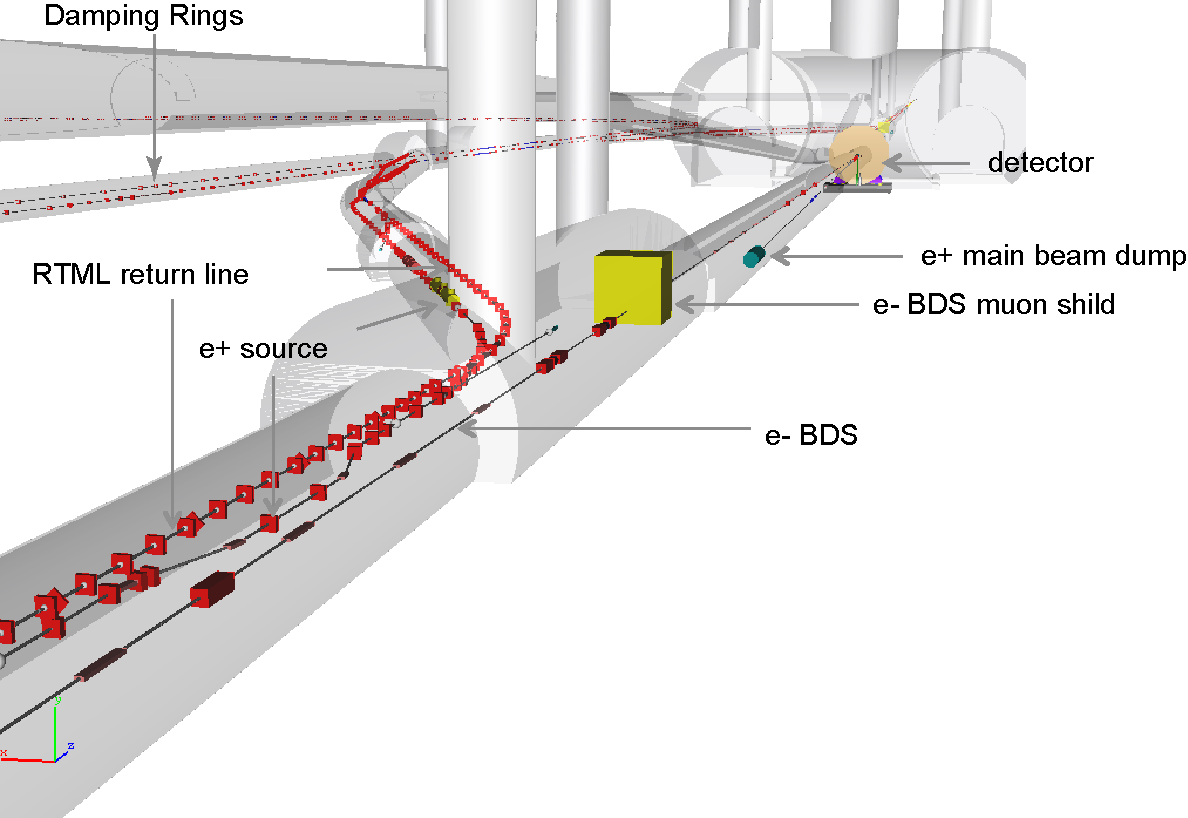
\includegraphics[scale=0.6]{./figures/ILC_region_centrale.pdf}
%       \caption{.}
%       \label{fig:ILC_schema_2}
%     \end{center}
%   \end{figure}
%   
%   \medskip
%   
%   Une \'etude g\'en\'erale de la physique \`a l'ILC men\'ee par un comit\'e de l'ICFA a conclu sur les principaux objectifs de physique qui devront être \'etudi\'es. Le GDE a alors établi les caract\'eristiques techniques principales de la machine \`a construire. 
  
  Les principales caract\'eristiques de la machine d\'erivant des objectifs de physique sont les suivants : 
  
  \medskip
  
  \renewcommand{\labelitemi}{$\bullet$}
  
  \begin{itemize}
   
   \item Une luminosit\'e qui doit conduire \`a $\int L dt = 500 \, fb^{-1}$ sur 4 ans,
   
   \item Une \'energie dans le centre de masse ajustable entre 200 et 500 $GeV$ (\'eventuellement option Giga-Z \`a 91 $GeV$ et Mega-W \`a 160 $GeV$),
   
   \item Une capacit\'e accrue \`a ajuster l'énergie dans le centre de masse entre 200 et 500 $GeV$,
   
   \item Une stabilit\'e de l'\'energie et une pr\'ecision sur celle-ci inf\'erieure \`a 0.1$\%$,
   
   \item Une polarisation des \'electrons $\geq 80 \%$.
   
   \end{itemize}
  
  \medskip  

%   De plus, le rapport de l'ICFA a identifi\'e diff\'erentes options qui devraient \^etre incluses dans la conception de la machine.
  
  De plus, il devra \^etre possible de mettre \`a jour la machine pour atteindre le $TeV$ dans le centre de masse. Un faisceau de positons polarisable est de plus souhaitable. Des caract\'eristiques plus d\'etaill\'ees de l'ILC sont list\'ees dans la table \ref{tab:paramILC}.
  
  \begin{table}[!htb]
  \begin{center}
  \begin{tabular}{|l|l|l|}  \hline
  Énergie max. dans le centre de masse & 500 & GeV  \\ \hline
  Pic de luminosit\'e & $\sim{2}\times10^{34}$ & $cm^{-2}s^{-1}$ \\ \hline
  Courant du faisceau & $9.0$ & mA \\ \hline
  Taux de r\'ep\'etition & $5$ & Hz \\ \hline
  Gradient moyen d'acc\'el\'eration & $31.5$ & MV/m \\ \hline
  Dur\'ee d'impulsion du faisceau & $0.95$ & ms \\ \hline
  Longueur totale du site & $31$ & km \\ \hline
  Puissance totale AC consomm\'ee & $\sim{230}$ & MW \\ \hline
  \end{tabular}
  \end{center}
  \caption{Principaux param\`etres du design de l'ILC \`a 500 $GeV$.}
  \label{tab:paramILC}
  \end{table}
  
%   L'ILC a \'et\'e con\c{c}u pour poss\'eder une \'energie réglable allant de 200 \`a 1000 $GeV$. Pour cela, les param\`etres de la machine ont \'et\'e optimis\'es en fonction du co\^ut, des risques et des performances de physiques. Le design cr\'e\'e est relativement conservatif et prend en compte certaines contraintes impos\'ees par les diff\'erents sous-syst\`emes d'acc\'el\'eration. Parmi celles-ci on peut lister des instabilit\'e de seuils (en particulier celle du nuage d'\'electrons dans l'anneau des positons), des \textit{temps de mont\'e} r\'ealistes pour les injecteurs et les extracteurs (kickers) et le désir de minimiser la circonf\'erence des anneaux.
  
  \medskip
  
  Pour r\'esumer l'ILC est un collisionneur d'\'electrons et de positons avec une \'energie r\'eglable entre 250 et 500 $GeV$ extensible \`a 1 $TeV$ dans le centre de masse. La technologie d'acc\'el\'eration radio-fr\'equence et la structure des faisceaux sont, de plus, adapt\'ees \`a la nature lin\'eaire du collisionneur. Apr\`es la description du complexe de l'acc\'el\'erateur, nous allons nous pencher sur les \'etudes physiques r\'ealisables \`a l'ILC. 
  
  %La production de positons dans l'ondulateur est d\'egrad\'e pour un faisceau d'électron d'énergie inf\'erieure \`a 150 $GeV$. Ainsi, pour des énergies dans le centre de masse inf\'erieures \`a 300 $GeV$ (faisceau d'électrons inf\'erieur \`a 150 $GeV$) le taux de r\'ep\'etition est augment\'e \`a 10 $Hz$. \\ la suite -> ?????? \\
  
  %La dur\'ee maximale de la pulsation du faisceau est contrainte \`a $\approx$ 1.6 $msec$.Il s'agit de ce qu'il est possible d'atteindre avec les klystrons multi-faisceaux \footnote{Les Klystrons convertissent et amplifient des faisceaux d'\'electrons en ondes radio-fr\'equence} (1.3 $GHz$ et 10 $MW$) et les modulateurs actuels. Le courant du faisceau est limit\'e par le nombre de klystrons (pic de puissance) et les modes d'ordre plus \'elev\'e.
    
  \subsection{Programme de physique}
  \label{sect:prog_physique}

%   Le mod\`ele standard de la physique des particules et de leurs interactions a pass\'e de nombreux tests de validation de la part de certains physiciens exp\'erimentateurs \cite{ALEPH:2010aa}. Le mod\`ele standard contient un m\'ecanisme de brisure de la symétrie \'electrofaible responsable de la masse des particules. Ce m\'ecanisme est appel\'e m\'ecanisme de Higgs et son boson vecteur, le boson de Higgs. Un candidat au boson de Higgs \'et\'e d\'ecouvert au LHC. Avec la faible pr\'ecision obtenue sur ses paramètres (masse, largeur, spin, couplages) \`a ce jour,  ce candidat est conforme au pr\'edictions du mod\`ele standard. Pour compl\'eter l'\'etude du mod\`ele standard et pour tenter de le d\'epasser, il faut mesurer avec pr\'ecision les propri\'et\'es de ces constituants et en particulier, le boson de Higgs. Cependant le mod\`ele standard n'explique pas plusieurs faits exp\'erimentaux importants et plusieurs questions restent encore en suspens :
% 
%   \medskip
% 
%   \renewcommand{\labelitemi}{$\bullet$}
% 
%   \begin{itemize}
%    \item La particule d\'ecouverte au LHC explique-t-elle enti\`erement l'origine de la brisure de la symétrie \'electro-faible et la masse des particules \'el\'ementaires ?
%    \item Pourquoi la particule d\'ecouverte au LHC a-t-elle cette masse et non une masse plus importante ? Ce probl\`eme est connu sous le nom de probl\`eme de hi\'erarchie.
%    \item Quelle est l'origine de la mati\`ere noire ?
%    \item Pourquoi l'univers est-il compos\'e de plus de mati\`ere que d'antimati\`ere ?
%    \end{itemize}
% 
%    \medskip

%    L'ILC permettra de chercher des r\'eponses \`a toutes ces questions.
   Comme nous l'avons d\'ej\`a vu, en juillet 2012, les collaborations ATLAS et CMS ont annonc\'e la d\'ecouverte d'une particule d'une masse de 125 $GeV/c^2$ compatible avec le boson de Higgs standard\cite{Aad:2012tfa, Chatrchyan:2012ufa}. Ces exp\'eriences du LHC continuent de raffiner leurs mesures sur les propri\'et\'es de cette nouvelle particule. Cependant, la pr\'ecision de ces mesures sera limit\'ee par la nature hadronique du collisionneur. De plus, les questions sur la physique au del\`a du mod\`ele standard restent encore en suspens et l'ILC sera le compl\'ement id\'eal au LHC pour tenter de r\'epondre \`a ces questions. Dans cette section nous allons d\'ecrire le programme de physique de l'ILC tel qu'il est d\'ecrit dans le \textit{TDR} \cite{Baer:2013cma}. Nous ferons ainsi une revue non exhaustive des mesures les plus importantes r\'ealisables \`a l'ILC.
   
   \medskip
   
   L'ILC \'etant un acc\'el\'erateur lin\'eaire, son \'energie dans le centre de masse est r\'eglable. Ainsi, diff\'erents programmes exp\'erimentaux pourront avoir lieu \`a l'ILC en fonction de l'\'energie disponible dans le centre de masse. Les diff\'erents programmes envisag\'es sont les suivants :
   
   \paragraph{91 GeV et 160 GeV :} \`A l'\'energie de 91 GeV on atteint la r\'esonance du boson $Z$ et \`a environ 160 GeV, on atteint le seuil pour de production de paires $W^+ W^-$ : $e^+ e^- \rightarrow W^+ W^-$. Comme l'ILC poss\'edera une luminosit\'e d'environ deux \`a trois ordre de grandeur au dessus de celle du LEP, cela permettra de mettre en place un programme \textit{GigaZ} et un programme \textit{MegaW}. L'objectif du programme \textit{GigaZ} est la mesure de l'asym\'etrie droite/gauche du Z et la mesure des couplages au Z avec une pr\'ecision d'un ordre de grandeur sup\'erieure compar\'ee \`a celle obtenue par le LEP. Le programme \textit{MegaW} vise quant \`a lui la mesure de la masse du W avec une pr\'ecision atteignant le $MeV/c^2$.
   
   \paragraph{250 GeV :} Cette \'energie correspond au pic de la section efficace du \textit{Higgstrahlung}. Ce dernier \'etant le nom donn\'e \`a la production de Higgs selon la r\'eaction $e^+ e^- \rightarrow Z h$. Avec $h$ le boson de Higgs de masse 125 $GeV/c^2$ d\'ecouvert au LHC. Que ce boson soit le boson de Higgs standard ou un autre boson, l'\'etude des couplages et des nombres quantiques de cette particule devrait \^etre r\'ealis\'ee avec pr\'ecision. La m\'ethode de la masse de recul devrait permettre une reconstruction de la masse de ce boson ind\'ependamment de toutes hypoth\`eses sur les produits de d\'esint\'egration du Higgs. (La masse manquante et les modes de d\'esint\'egration inattendus \'etant pris en compte). Nous reviendrons sur cette m\'ethode un peu plus loin.
   
   \paragraph{350-400 GeV :} Le seuil de production de paires $t\overline{t}$ apparaît aux alentour de 350 $GeV$. A cause de son très faible temps de vie, le quark top et son anti-particule ne poss\`edent pas d'\'etat li\'e (pas de particule compos\'ee de quark ou d'anti-quark top). Cependant, la section efficace de production de paires $t\overline{t}$ exhibe une forme particuli\`ere pr\`es du seuil de production. Cette forme est tr\`es pr\'ecis\'ement pr\'edite par des calculs de QCD perturbative. Un balayage en \'energie autour du seuil devrait permettre de reconstituer cette forme. La masse du quark top pourra alors \^etre mesur\'ee avec une pr\'ecision d'environ 100 $MeV/c^2$. La mesure pr\'ecise des \'etats finals au seuil de production et aux \'energies plus hautes livreront des mesures de pr\'ecision contraignant la brisure de la symétrie \'electrofaible. Au alentour de cette \'energie la section efficace de production de Higgs par fusion $WW$ devient importante. La mesure de la r\'eaction $e^+ e^- \rightarrow \nu \nu h$ devrait fournir une mesure pr\'ecise du couplage $hWW$. En effet, la section efficace de ce processus augmente avec l'\'energie dans le centre de masse (voir figure \ref{fig:energyHiggs}). Cette production de boson de Higgs offrira une statistique \'elev\'ee pour l'\'etude des d\'esint\'egrations rares du boson de Higgs. De plus une mesure fine des couplages au W \`a l'aide de la r\'eaction $e^+ e^- \rightarrow W^+ W^-$ permettra l'\'etude d'une d\'eviation de ces couplages par rapport au mod\`ele standard.
   
  \begin{table}[htb!] 
  \footnotesize{
  \begin{center}
  \begin{tabular}{rccc}
  \'Energie             &   R\'eaction  &  Objectif physique     
  \\  \hline \hline
  91~GeV            &       $e^+e^-  \to Z$     &      
   mesures ultra-pr\'ecises du mod\`ele \'electrofaible        \\   \hline
  160~GeV            &       $e^+e^-  \to WW$     &
  mesure ultra-pr\'ecise de la masse du $W$         \\   \hline
  250~GeV         &    $e^+e^-  \to Z h$     &      mesures pr\'ecises des couplages au Higgs           \\ 
			    \hline
  350--400~GeV         &      $e^+e^-  \to t\bar t$        &  
    mesures de la masse du quark top et de ses couplages                \\
    &    $ e^+e^-  \to WW$     &     mesures pr\'ecises des couplages au $W$             \\ 
			&     $ e^+e^-  \to \nu\bar\nu h $   & 
  mesures pr\'ecises des couplages au Higgs     \\   \hline
  500~GeV         &      $e^+e^-  \to f\bar f   $       &   
  recherche précise du $Z'$      \\ 
      &  $ e^+e^-  \to t\bar t h$    &      mesures des couplages Higgs-top      \\
			  &      $e^+e^-  \to Z h h $       &     mesure de l'auto-couplage du Higgs            \\
			&   $   e^+e^- \to  \tilde \chi \tilde \chi$  &
			recherche de la supersym\'etrie   \\  
			&    $  e^+e^- \to AH, H^+H^-  $  &
			recherche d'\'etats \'etendus du Higgs   \\  \hline
  700--1000~GeV &        $ e^+e^-  \to \nu\bar \nu hh $ & 
	  mesures des autocouplages du Higgs     \\ 
			    &    $e^+e^-  \to \nu\bar \nu VV$ &  recherche d'un Higgs composite  \\ 
			    &    $e^+e^-  \to \nu\bar \nu t\bar t$ &
			    recherche de Higgs et top composites  \\
			    &    $e^+e^-  \to \tilde t \tilde{ t}^* $ &
			  recherche de la supersym\'etrie  \\
			    \hline
  \end{tabular}
  \end{center} }
  \caption{Principaux processus physiques \'etudi\'es \`a l'ILC pour diff\'erentes \'energies dans le centre de masse. Le tableau indique les diff\'erentes réactions du mod\`ele standard accessibles en fonction de l'augmentation en \'energie, ainsi que les principaux objectifs physiques. Une r\'eaction list\'ee \`a une \'energie donn\'ee sera aussi \'etudi\'ee pour toutes les \'energies plus \'elev\'ees.}
  \label{tab:ILCprogramX}
  \end{table}
   
   \paragraph{500 GeV :} A cette \'energie l'ILC fonctionnera \`a son \'energie et \`a sa luminosit\'e nominale. Les donn\'ees collect\'ees permettront alors d'am\'eliorer les pr\'ecisions sur les mesures des processus sus-mentionn\'es. A cette \'energie, l'\'etude des r\'eactions $e^+ e^- \rightarrow f \overline{f}$ ou $f$ peut \^etre un quark ou un lepton, offre la possibilit\'e d'\'etudier la physique au delà du mod\`ele standard. Du fait de leur simplicit\'e, les \'etats finals de ces processus sont facilement distinguables exp\'erimentalement. De plus, les calculs perturbatifs correspondant, bas\'es sur le mod\`ele standard, ont d\'ejà \'et\'e r\'ealisés et donnent des r\'esultats tr\`es pr\'ecis. De faibles d\'eviations sur les pr\'edictions du mod\`ele standard pourraient permettre d'explorer une nouvelle physique \`a des \'echelles d'\'energie bien sup\'erieure \`a celle du centre de masse. L'existence du boson $Z'$, la nature composite des fermions ou encore certains mod\`eles \`a dimensions suppl\'ementaires pourront \^etre test\'es. Le d\'etecteur de vertex jouera un r\^ole primordial dans l'identification des saveurs mises en jeu. De plus, de nouvelles particules pourront \^etre recherch\'ees comme certaines particules supersym\'etriques ou comme d'autres \'etats d'un secteur de Higgs composite. De plus, \`a cette \'energie l'\'etude du couplage du quark top au Higgs devient possible.
%    Cette recherche de nouvelles particules est tr\`es difficile au LHC pour certaines gammes de param\`etres.
   
   \paragraph{1 TeV :} \`A cette \'energie de fonctionnement, envisag\'ee apr\`es une mise \`a jour de l'ILC, de nombreuses nouvelles mesures seront possibles. Ces mesures permettront entre autre d'explorer : le couplage du Higgs au quark top, les auto-couplages du Higgs et les mod\`eles de Higgs composite. De nouvelles particules exotiques pourront de plus \^etre recherch\'ees. Les donn\'ees produites permettront aussi d'am\'eliorer la pr\'ecision des mesures d\'ej\`a r\'ealis\'ees \`a des \'energies dans le centre de masses inf\'erieures.
   
% Le quark top est le plus massif des six quarks que nous connaissons. Sa grande masse, comparable à celle d'un atome d'or, lui confère une caractéristique particulière dans la famille des quarks : il n'existe pas d'état lié (donc de particule) avec un quark top (ou antitop). C'est en détectant ses produits de désintégration que l'on mesure les caractéristiques de ce quark.

  \medskip

  Le tableau \ref{tab:ILCprogramX} r\'esume tous ces programmes. Apr\`es avoir r\'ealis\'e une revue des \'etudes possibles \`a l'ILC nous allons nous pencher plus particuli\`erement sur la physique du Higgs, du top et la supersym\'etrie \`a l'ILC.

   \subsubsection{Physique du Higgs}
  
   La premi\`ere phase du programme de recherche sur le Higgs sera constitu\'ee par la mesure pr\'ecise des propri\'et\'es du boson de Higgs d\'ecouvert au LHC. L'objectif sera de savoir si ce boson est vraiment compatible avec le mod\`ele standard ou si des diff\'erences apparaissent.
  
  \medskip

   La premi\`ere \'etape de notre cheminement consiste \`a savoir quels sont les modes de production de Higgs du mod\`ele standard observables \`a L'ILC. Pour cela nous allons discuter les sections efficaces de production du Higgs standard \`a l'ILC. La figure \ref{fig:feynmanHiggs2} repr\'esente les diagrammes de \textit{Feynman} des trois processus majoritaires de production du Higgs \`a l'ILC.
   
  \begin{figure}[!htb]
    \begin{center} 
      \includegraphics[scale=0.40]{./figures/feynman_Higgs.png}
      \caption{Diagrammes de \textit{Feynman} pour les 3 processus majeurs de production de Higgs \`a l'ILC : $e^+ e^- \rightarrow Z h$ (\`a gauche), $e^+ e^- \rightarrow \nu \overline{\nu} h$ (au centre), et $e^+ e^- \rightarrow e^+ e^- h$ (\`a droite). }
      \label{fig:feynmanHiggs2}
    \end{center}
  \end{figure}
   
  \begin{figure}[!htb]
    \begin{center} 
      \includegraphics[scale=0.40]{./figures/energy_Higgs.jpg}
      \caption{Section efficace de production pour le Higgstrahlung ($e^+ e^- \rightarrow Z h$), la fusion WW ($e^+ e^- \rightarrow \nu \overline{\nu} h$) et la fusion ZZ ($e^+ e^- \rightarrow e^+ e^- h$) en fonction de l'\'energie dans le centre de masse, pour une masse du Higgs de 125 $GeV$, et pour une polarisation de faisceau ($P_{e^-}$, $P_{e^+}$) = ($-0.8$, $+0.2$). }
     \label{fig:energyHiggs}
     \end{center}
  \end{figure}
   
   D'autres processus existent, cependant ils ont une section efficace d'au moins un ordre de grandeur inf\'erieur \`a la fusion $ZZ$ et n'apparaissent qu'\`a partir de 350-500 $GeV$ dans le centre de masse (voir figure \ref{fig:crossSectionHiggs}). En figure \ref{fig:energyHiggs} est illustr\'ee la section efficace de production des trois processus majoritaires en fonction de l'\'energie dans le centre de masse, obtenue pour une polarisation de faisceau $(Pe^- , Pe^+ ) = (-0.8 , +0.2)$. La section efficace maximale de la r\'eaction $e^+ e^- \rightarrow Zh$ est obtenue aux alentours de 250 GeV dans le centre de masse. Elle vaut environ 220 $fb$. Cette r\'eaction porte le nom de Higgstrahlung. \`A cette \'energie la fusion $W^+W^-$ ($e^+ e^- \rightarrow \nu \overline{\nu} h$) poss\`ede une section efficace un ordre de grandeur au dessous. Cependant, alors que le Higgstrahlung diminue avec l'augmentation de l'\'energie disponible dans le centre de masse \`a partir de 250 GeV, la fusion $WW$ augmente avec la hausse en \'energie. Ainsi aux alentours de 500 GeV le Higgstrahlung et la fusion $WW$ ont environ la même section efficace (environ 120 $fb$). A plus haute \'energie, la section efficace de fusion $WW$ augmente encore et le Higgstrahlung d\'ecro\^it. Ainsi avec l'\'energie maximale de 1 $TeV$ atteignable \`a l'ILC, la section efficace de fusion $WW$ vaut environ 400 $fb$ et celle du Higgstrahlung 20 $fb$. La fusion $ZZ$ est quant \`a elle minoritaire. Elle passe d'environ quelques $fb$ \`a 250 GeV \`a 20 $fb$ \`a 1 $TeV$. Ainsi, plusieurs programmes de physique selon que l'on soit \`a une \'energie de 250, 500 ou 1000 $GeV$ dans le centre de masse sont r\'ealisables. 
   
   \medskip
   
   \begin{figure}[!htb]
     \begin{center} 
       \includegraphics[scale=0.35]{./figures/recoil_mass_Higgs.png}
       \caption{ R\'esultats d'une simulation de 250 $fb^{-1}$ du Higgsstrahlung $e^+ e^- \rightarrow Z h$ avec \`a gauche $Z \rightarrow \mu^+ \mu^-$  et \`a droite $Z \rightarrow e^+ e^- (+n \gamma)$ comme attendu dans le d\'etecteur ILD de l'ILC. Ces r\'esultats sont montr\'es pour une polarisation $P(e^+ , e^-) = (+0.3 , -0.8)$ (TDR Volume Physics \cite{Behnke:2013lya} p288)}
     \label{fig:simuILC}
     \end{center}
  \end{figure}

% TDR page 288
  
   Le programme de l'ILC devrait donc commencer par l'exploitation du pic du Higgsstrahlung vers 250 $GeV$. Pour cela, la masse du Higgs sera reconstruite grâce \`a sa masse de recul $M_H$. L'int\'er\^et de cette m\'ethode repose sur le fait que la masse calcul\'ee est ind\'ependante de toute hypoth\`ese sur les produits de d\'esint\'egration du Higgs. Celui-ci peut alors se d\'esint\'egrer en invisible ou en particules exotiques sans que cela influe sur la mesure de sa masse. La masse de recul du Higgs est calcul\'ee selon la relation suivante :
   
   \begin{equation}
    M_H^2 = s + M_Z^2 - 2 \sqrt{s}(E_1 + E_2)
   \end{equation}
 
   o\`u $M_H$ est la masse de recul du boson de Higgs, $M_Z$ la masse du boson $Z$ et $E1$ et $E2$ sont les \'energies des produits de d\'esint\'egration du $Z$. La figure \ref{fig:simuILC} repr\'esente la simulation bas\'ee sur 250 $fb^{-1}$ de donn\'ees, de la masse de recul du Higgs dans le cas ou le Z se d\'esint\`egre en une paire de muons $\mu^+ \mu^-$ (ou $e^+ e^-$). La m\'ethode de la masse de recul comme illustr\'ee en figure \ref{fig:simuILC} permet d'obtenir une pr\'ecision statistique de l'ordre de 40 $MeV$ sur la masse de recul du Higgs pour le canal $Z \rightarrow \mu^+ \mu^-$ avec une \'energie de 250 $GeV$ dans le centre de masse et 250 $fb^{-1}$ de donn\'ees simul\'ees. Une pr\'ecision de l'ordre de 80 $MeV$ est obtenue dans les m\^emes conditions de simulation pour le canal $Z \rightarrow e^+ e^-$. La combinaison des deux r\'esultats donne une pr\'ecision sur la mesure d'environ 32 $MeV$ \cite{Abe:2010aa} \cite{Li:2012taa}.
   
   \medskip
   
   \begin{figure}[!htb]
     \begin{center} 
       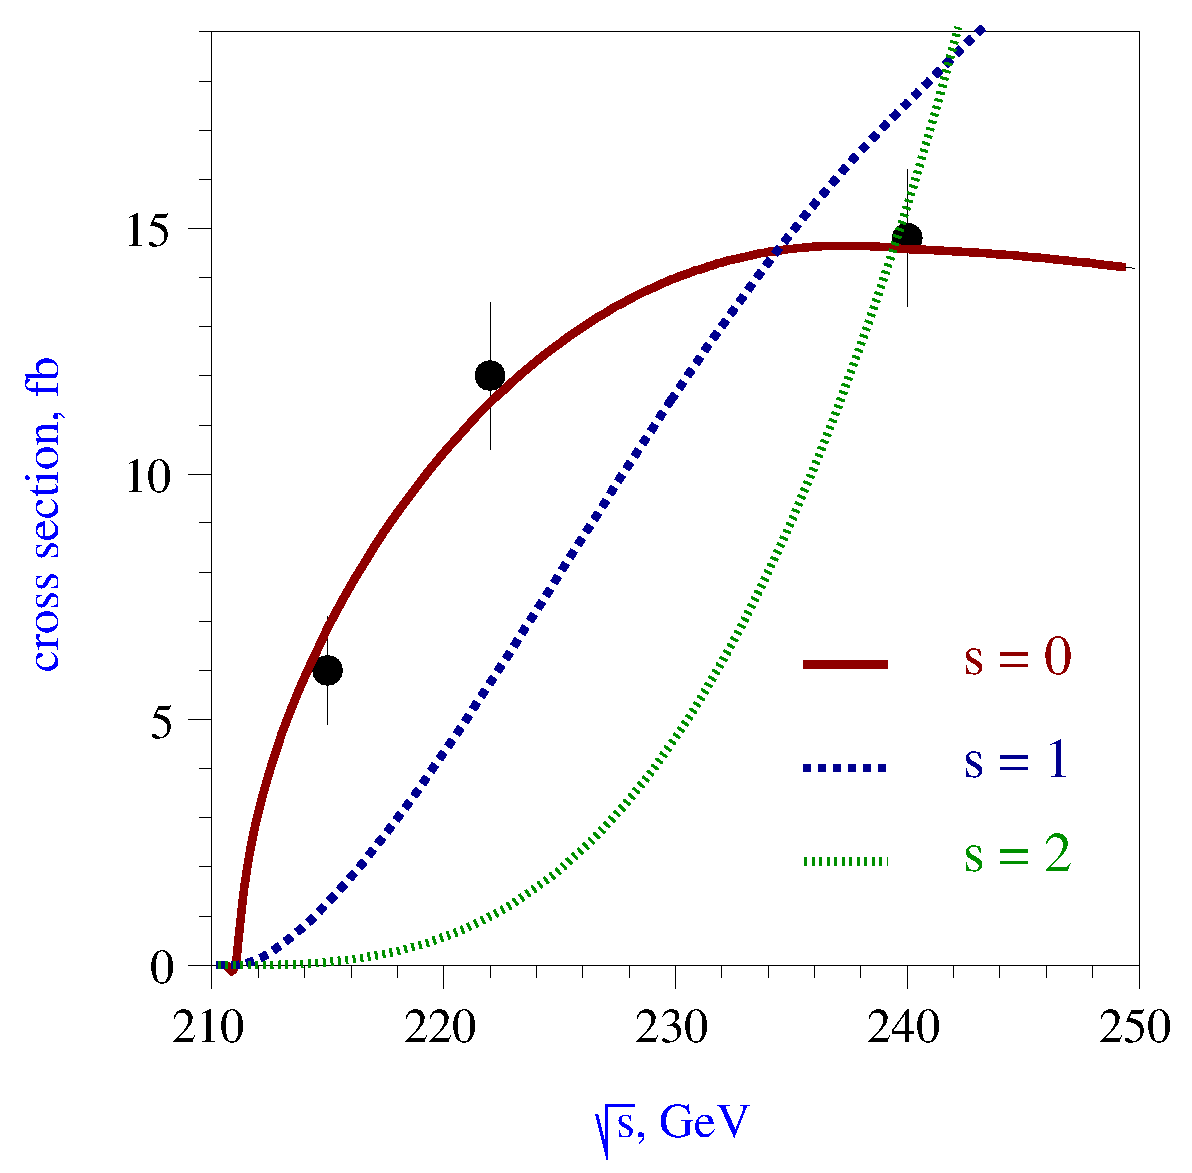
\includegraphics[scale=0.35]{./figures/higgs_spin1.eps}
       \caption{ Comportement de la section efficace $e^+ e^- \rightarrow Zh$ au seuil de production, en fonction du spin et de la valeur de CP. Les trois courbes indiquent le comportement th\'eorique de la section efficace au seuil de production pour $J^P$ = $0^+$ , $1^-$, et $ 2^+$. 3 points de mesures avec 20 $fb^{-1}$ de donn\'ees permettent de distinguer les diff\'erentes possibilit\'es. \cite{Dova:2003py} }
     \label{fig:spinHiggs}
     \end{center}
   \end{figure}
   
   Le programme de mesure \`a 250 $GeV$ inclura la mesure de la masse mais aussi du spin et de CP pour le boson de Higgs. Ainsi, l'ILC procurera un test complémentaire au LHC pour la mesure du spin du boson de Higgs. La m\'ethode de mesure est bas\'ee sur le comportement au seuil de production pour la section efficace du Higgstrahlung $e^+ e^- \rightarrow Zh$. Cette section efficace ne varie pas de la m\^eme mani\`ere selon les valeurs du spin et de CP pour le boson de Higgs. La possibilit\'e d'un spin 1 a \'et\'e exclue par l'observation du canal $h\rightarrow \gamma \gamma$ au LHC. Pour un boson de Higgs de spin 0, le comportement au seuil de la section efficace $e^+ e^- \rightarrow Zh$ \`a l'ILC varie comme lin\'eairement pour une valeur de CP paire et comme $x^3$ pour une valeur de CP impaire (voir figure \ref{fig:spinHiggs} \cite{Dova:2003py}). Pour un boson de Higgs de spin 2, la section efficace au seuil augmente comme $x^3$. Pour des spins plus \'elev\'es, la section efficace au seuil augmentera selon des puissances de $x^n$ plus grande que 3. Des mesures de la section efficace juste au dessus du seuil de production devraient permettre de trancher entre toutes ces possibilit\'es. Trois points de mesure nécessitant 20 $fb^{-1}$ de donn\'ees permettront de s\'eparer toutes les possibilit\'es et donc d'obtenir le spin et la valeur de CP \cite{Dova:2003py}.   
   
   \medskip
% Cette voie de d\'esint\'egration impose une valeur positive pour la conjugaison de charge.


   \begin{figure}[!htb]
   \renewcommand{\figurename}{Table}
   \begin{center} 
      \includegraphics[scale=0.38]{./figures/table_BR_Higgs_MS.png}
      \caption{ Pr\'ecision sur les rapports de branchement pour un Higgs standard \`a 120 $GeV/c^2$, obtenue avec une simulation compl\`ete du d\'etecteur, pour une \'energie dans le centre de masse de 250 $GeV$ et une luminosit\'e int\'egr\'ee $L = 250 \, fb^{-1}$ et une polarisation des faisceaux $(e^- , e^+ ) = (-0.8, +0.3)$. Les erreurs sur les rapports de branchements incluent des erreurs de $2.5 \%$ sur $\sigma$. \cite{Ono:2013sea}}
     \label{fig:BR_SM_Higgs}
     \end{center}
  \end{figure}
  
   Les taux de d\'esint\'egration du boson de Higgs pourront \^etre mesur\'es avec pr\'ecision. Le tableau \ref{fig:BR_SM_Higgs} indique les rapports de branchement pour les diff\'erents modes de d\'esint\'egration pour le Higgs du mod\`ele standard. Les mesures qui seront r\'ealis\'ees \`a l'ILC, incluront  les d\'esint\'egrations invisibles ou les \'etats finaux inhabituels. Compar\'e au LHC o\`u de tels \'ev\`enements sont tr\`es difficilement s\'eparables du bruit de fond du mod\`ele standard, l'ILC permettra ces mesures avec une grande pr\'ecision. Dans le mod\`ele standard, les couplages du Higgs aux fermions sont proportionnels \`a la masse des fermions :
   
   \begin{equation}
    g_{hf\overline{f}} = \cfrac{m_f}{v}
   \end{equation}
  
    Et les couplages du Higgs aux bosons de jauge sont proportionnels \`a la masse au carr\'e de ces bosons. Avec $V = W , Z$, on a : 
    
    \begin{equation}
     g_{hVV} = \cfrac{2 m_V^2}{v}
    \end{equation}

%    \begin{figure}[!htb]
%      \begin{center} 
%        \includegraphics[scale=0.50]{./figures/Chapter_Theory_figs_mass-coupling1TeV.png}
%        \caption{ Les pr\'edictions des mesures des couplages au Higgs \`a l'ILC sont indiqu\'ees sur cette figure. La quantit\'e de donn\'ees utilis\'ee prend en compte l'ensemble des programmes envisag\'ees \`a l'ILC y compris celui \`a 1 $TeV$. }
%      \label{fig:HiggsCoupling}
%      \end{center}
%    \end{figure}
 
   Ainsi, des mesures de grande pr\'ecision des taux de d\'esint\'egration du boson de Higgs selon diff\'erentes voies (quarks, leptons et bosons) permettront de savoir si seul le champ de Higgs conf\`ere leur masse aux particules \'el\'ementaires ou si d'autres particules partagent le rôle de g\'en\'erateur de la masse. Il existe en effet plusieurs sc\'enarios de nouvelle physique qui g\'en\`erent des d\'eviations sur ces valeurs inf\'erieures \`a 10$\%$ par rapport au mod\`ele standard \cite{Gupta:2013}. On attirera l'attention du lecteur sur les voies de d\'esint\'egration $h \rightarrow b\overline{b}$ et $h \rightarrow c\overline{c}$ repr\'esentant respectivement environ $65.7\%$ et $3.6\%$ des d\'esint\'egrations du Higgs standard. Nous focaliseront aussi l'attention sur le canal $\tau^- \tau^+$ repr\'esentant environ $8\%$ de ces d\'esint\'egrations. Toutes ces saveurs devront \^etre reconstruites gr\^ace au d\'etecteur de vertex. 
   
   \medskip
   
   La largeur du boson de Higgs du mod\`ele standard \'etant estim\'ee \`a environ 4 $MeV/c^2$, une mesure directe aussi pr\'ecise ne pourra pas \^etre effectu\'ee \`a l'ILC. Cependant, la section efficace du processus $e^+ e^- \rightarrow Zh$ est proportionnelle au couplage $g_{hZZ}$ au carr\'e. Comme la largeur du processus de d\'esint\'egration $h \rightarrow ZZ^*$, $\Gamma(h \rightarrow ZZ^*)$, est proportionnelle \`a la constante de couplage $g_{hZZ}$ au carr\'e, la section efficace $e^+ e^- \rightarrow Zh$ est aussi proportionnelle \`a la largeur $\Gamma(h \rightarrow ZZ^*)$ \cite{Durig:2014lfa}. Cette derni\`ere largeur peut donc \^etre calcul\'ee \`a partir de la mesure pr\'ecise de la section efficace du processus $e^+ e^- \rightarrow Zh$. Étant donn\'e le rapport de branchement $BR(h \rightarrow ZZ^*)$ obtenu gr\^ace \`a la m\'ethode de la masse de recul, la largeur du boson de Higgs est donn\'ee par : 
   
   \begin{equation}
    \Gamma_{tot} = \dfrac{\Gamma(h \rightarrow ZZ^*)}{BR(h \rightarrow ZZ^*)}
   \end{equation}
 
   Le rapport de branchement $BR(h \rightarrow ZZ^*)$ \'etant faible ($\approx 1.7 \%$), une statistique importante est n\'ecessaire afin d'obtenir une mesure pr\'ecise. \`A 250 GeV avec 250 $fb^{-1}$ de donn\'ees collect\'ees, une pr\'ecision d'environ 26\% est attendue pour $BR(h \rightarrow ZZ^*)$. Afin d'augmenter la pr\'ecision sur la mesure de la largeur du Higgs l'utilisation du mode de d\'esint\'egration $h \rightarrow WW^*$ peut aussi \^etre utilis\'e. Une pr\'ecision sur la largeur du Higgs d'environ 2$\%$ pourra \^etre atteinte avec 250 $fb^{-1}$ de donn\'ees \`a 250 $GeV$ plus 500 $fb^{-1}$ de donn\'ees \`a 500 $GeV$.

   \medskip
   
   Dans la région d'\'energie 350-400 $GeV$ dans le centre de masse et plus haut, la r\'eaction $e^+ e^- \rightarrow WW$ permettra de sonder le mod\`ele standard \`a haute \'energie. Au fur et \`a mesure que l'\'energie monte, le processus de fusion $WW$ ($e^+ e^- \rightarrow \nu \overline{\nu} h$) cro\^it et une mesure plus pr\'ecise du couplage $hWW$ est alors possible. Il s'agit d'une des valeurs cruciales dans l'\'etude pr\'ecise du boson de Higgs.
   
   \medskip
  
  \begin{figure}[!htb]
    \begin{center} 
      \includegraphics[scale=0.60]{./figures/tripleH_diagram.png}
      \caption{Diagrammes de \textit{Feynman} des processus $e^+ e^- \rightarrow Zhh$ et $e^+  e^- \rightarrow \nu_e \overline{\nu_e} hh$. Triple auto-couplage du Higgs.}
     \label{fig:triple-self_couplingHiggs}
     \end{center}
  \end{figure}    

   \`A 500 $GeV$ dans le centre de masse, deux processus importants \`a la compr\'ehension de la brisure de la sym\'etrie \'electrofaible deviennent accessibles \`a la mesure, le couplage de Yukawa du quark top et le terme d'auto-couplage triple du Higgs. La mesure du couplage de Yukawa du quark top sera accessible \`a partir de la r\'eaction $e^+ e^- \rightarrow t \overline{t} h$. La mesure de ce couplage permettra de mieux comprendre le m\'ecanisme de la g\'en\'eration des masses des fermions. 
   
   Une pr\'ecision de $\Delta g_t /g_t \approx 10\%$ sera possible avec une reconstruction du signal $e^+ e^- \rightarrow ttH$ en 6-jets + lepton et 8-jets, avec un Higgs \`a 120 GeV, une polarisation des faisceaux $(Pe^- , Pe^+ ) = (-0.8, +0.3)$ , et une luminosit\'e int\'egr\'ee de 1 $ab^-{1}$ \cite{Yonamine:2011jg}.

%    le canal $e^+ e^- \rightarrow ttH \rightarrow bW^- bW^+ b\overline{b}$ pour 1 $ab^{-1}$ de luminosit\'e int\'egr\'ee \`a 500 $GeV$ et pour un boson de Higgs de 120 GeV \cite{Tabassam:2012it}. Une pr\'ecision de $\Delta g_t /g_t \approx 28\%$ sera possible avec le canal $e^+ e^- \rightarrow ttH \rightarrow bW^- bW^+ b\overline{b}$ pour 1 $ab^{-1}$ de luminosit\'e int\'egr\'ee \`a 500 $GeV$ et pour un boson de Higgs de 120 GeV \cite{Tabassam:2012it}. 
   
   Les processus $e^+ e^- \rightarrow Zhh$ et $e^+  e^- \rightarrow \nu_e \overline{\nu_e} hh$ (voir figure \ref{fig:triple-self_couplingHiggs}) dont les sections efficaces sont tr\`es faibles de l'ordre de $0.1$ et $10^{-2}$ $fb$ (voir figure \ref{fig:crossSectionHiggs}) permettront d'estimer le terme $\lambda$ d'auto-couplage triple du Higgs. On rappelle que dans le mod\`ele standard : 
   
   \begin{equation}
    g_{hhh} = \cfrac{3}{2} \lambda v = \cfrac{3 m_h^2}{v}
   \end{equation}

   \`A la fin du programme de physique de l'ILC, une pr\'ecision de $\Delta \lambda / \lambda$ = 0.44 est atteignable avec $2 ab^{-1}$ de donn\'ees \`a 1 TeV. (TDR, Physics, page 37).
   
   \medskip
  
  \begin{figure}[!htb]
    \begin{center} 
      \includegraphics[scale=0.38]{./figures/BR_Higgs_500GeV.png}
      \caption{Pr\'ecisions sur les rapports de branchement mesur\'es \`a l'ILC en fonction des statistiques engrang\'ees \`a 250, 500, et 250+500 GeV.(source : TDR : Physics, page 39)}
     \label{fig:BR_500GeV}
     \end{center}
  \end{figure} 
   
   Toujours \`a 500 $GeV$, la d\'etermination des rapports de branchement du Higgs sera plus pr\'ecise en raison de l'augmentation de la statistique. La figure \ref{fig:BR_500GeV} r\'esume les pr\'ecisions atteignables en fonction de la luminosit\'e int\'egr\'ee \`a 250 et 500 $GeV$.   
   
%    De plus, pour tester si le Higgs est standard ou non, un test important est celui du potentiel de Higgs. Le potentiel du mod\`ele standard donne lieu \`a des auto-couplages triples et quadruples du Higgs. L'ILC mesurera le terme d'auto-couplage triple \cite{Baer:2013cma}.
   
   \medskip

  \begin{figure}[!htb]
    \begin{center} 
      \includegraphics[scale=0.40]{./figures/cross_section_prod_Higgs_ILC.png}
      \caption{Section efficace de production du boson de Higgs. Les processus minoritaires sont cette fois-ci indiqu\'es.}
     \label{fig:crossSectionHiggs}
     \end{center}
  \end{figure} 
   
   Comme la figure \ref{fig:crossSectionHiggs} le montre, la section efficace de la r\'eaction $e^+ e^- \rightarrow t \overline{t} h$ augmente avec l'\'energie dans le centre de masse et atteint son maximum \`a environ 800 $GeV$. Cette section efficace d\'ecroît ensuite tr\`es l\'eg\`erement, mais reste proche de son maximum \`a 1 $TeV$. De plus, \`a 1 $TeV$ le bruit de fond $e^+ e^- \rightarrow t\overline{t}$ est devenu moins important. Une am\'elioration sur la pr\'ecision du coulage de Yukawa du quark top est alors possible. Une estimation r\'ecente r\'ealis\'ee grâce \`a une simulation compl\`ete, donne une pr\'ecision statistique de $4.0\%$ sur la valeur du couplage de Yukawa du top avec un Higgs standard de 125 $GeV$ et 1 $ab^{-1}$ de donn\'ees \`a 1 $TeV$ (voir TDR : physics, page 40).
   
   \medskip
   
   Toujours \`a 1 $TeV$ la fusion $WW$ est devenue le canal majoritaire de production de boson de Higgs, et en optimisant la polarisation des faisceaux \`a $(Pe^- , Pe^+ ) =  (-0.8, +0.2)$, on peut atteindre une section efficace de production de 400 $fb$ pour un Higgs de 125 $GeV$. Ainsi, avec 1 $ab^{-1}$ de donn\'ees, on obtient $4 \times 10^5$ \'ev\'enements contenant un Higgs. Cela permettra de mesurer le canal de d\'esint\'egration $h \rightarrow \mu^+ \mu^-$. Des simulations r\'ecentes montrent qu'il sera possible de mesurer la section efficace $\sigma BR(h \rightarrow \mu^+ \mu^-)$ avec une pr\'ecision d'environ $32\%$ pour un Higgs \`a 125 $GeV$, une polarisation $ P(-0.8, +0.2)$ et 1 $ab^{-1}$ \`a 1 $TeV$ (TDR, Physics : page 40).
   
   \medskip
   
   De plus, la section efficace du processus $e^+ e^- \rightarrow \nu \overline{\nu} h h$ devient beaucoup plus importante \`a 1 $TeV$ qu'\`a 500 $GeV$. Elle atteint environ 0.1 $fb$ \`a 1 $TeV$ (voir figure \ref{fig:crossSectionHiggs}). L'analyse de ce canal, coupl\'ee avec celle du canal $e^+ e^- \rightarrow Z h h$ permettra d'am\'eliorer la pr\'ecision sur la mesure de l'auto-couplage du Higgs. Une simulation compl\`ete r\'ecente donne une pr\'ecision $\Delta \lambda / \lambda \approx 0.21$. Ce r\'esultat est obtenu pour le canal $e^+ e^- \rightarrow \nu \overline{\nu} h h$ avec 2 $ab^{-1}$ \`a 1 $TeV$ et une polarisation $(P e^- , P e^+ ) = (-0.8, +0.2)$ (voir TDR : physics, page 41).
   
   \medskip

   \begin{figure}[!htb]
    \begin{center} 
      \includegraphics[scale=0.40]{./figures/Comparaison_couplage_1TeV.png}
      \caption{Pr\'ecisons sur les couplages du Higgs en fonction de l'exp\'erience, de l'\'energie dans le centre de masse et de la luminosit\'e int\'egr\'ee. \cite{Peskin:2012we}}
     \label{fig:Comp_BR_1000GeV}
     \end{center}
  \end{figure} 
   
   La figure \ref{fig:Comp_BR_1000GeV}, donne les diff\'erentes pr\'ecisions sur les couplages du Higgs. Sont mentionn\'ees les pr\'ecisions pour le LHC \`a 300 $fb^{-1}$ (avec 1 seul d\'etecteur), l'ILC \`a 250 GeV avec 250 $fb^{-1}$, l'ILC \`a 500 GeV avec 500 $fb^{-1}$ et l'ILC \`a 1000 GeV avec 1000 $fb^{-1}$ \cite{Peskin:2012we}. Cette figure r\'esume \`a elle toute seule l'int\'er\^et de l'ILC. Les pr\'ecisions obtenues \`a l'ILC permettront de tester si les param\`etres mesur\'es sont standards ou s'ils d\'evient du mod\`ele standard. La pr\'ecision de ces mesures constitue donc une sonde sur la physique au delà du mod\`ele standard.
   
   \subsubsection{Supersym\'etrie}
   
   Comme nous l'avons vu, la supersymétrie permet de r\'esoudre le probl\`eme de hi\'erarchie, elle postule un bon candidat de particule de mati\`ere noire et permet de faire se rejoindre les constantes de couplage des interactions fondamentales \`a l'\'echelle de grande unification.
   
   \medskip
   
   Actuellement (fin 2014), aucune preuve de particule supersym\'etrique n'a été identifiée au LHC, avec une \'energie de 8 $TeV$ dans le centre de masse. La recherche de telles particules au LHC continuera pour des \'energies de 13/14 TeV dans le centre de masse \`a partir de 2015. On notera que le LHC est particuli\`erement sensible aux super-partenaires color\'es.
   
   \medskip
   
   L'ILC sera un acc\'el\'erateur compl\'ementaire du LHC pour la recherche de supersymétrie. Il pourra permettre la mesure pr\'ecise d'\'eventuelles particules supersym\'etriques d\'ecouvertes au LHC. De plus, l'ILC permet de tester des espaces de param\`etres o\`u le LHC ne poss\`ede qu'une faible sensibilit\'e. Beaucoup de ces hypoth\'etiques nouvelles super-particules interagissent uniquement par l'interaction faible (neutralinos, jauginos). Leur faible niveau de production compar\'e aux particules interagissant par interaction forte, et le bruit de fond important des collisionneurs hadroniques, en font des particules difficilement observables au LHC. Ce bruit de fond et ce faible taux de production ne sont pas applicables au cas de l'ILC, et celui ci permettra de d\'ecouvrir et d'identifier ces particules si l'\'energie dans le centre de masse est assez haute pour les produire. Certaines particules supersym\'etriques ne lib\'erant qu'une tr\`es faible \'energie lors de leur d\'esint\'egration, le LHC, aura des difficult\'es \`a les d\'etecter. Ainsi, l'ILC gr\^ace \`a son faible bruit de fond pourrait d\'etecter des particules supersym\'etriques pass\'ees inaperçues au LHC. Pour finir, si de telles particules supersym\'etriques \'etaient d\'ecouvertes \`a l'ILC, ce dernier devrait fournir des mesures de pr\'ecisions sur les param\`etres les caract\'erisant, ce qui devrait fortement contraindre les mod\`eles th\'eoriques existants.

% \`a ses d\'etecteurs tr\`es pr\'ecis
   %   De nouvelles particules associ\'ees au champ de Higgs, \`a la mati\`ere noire mais aussi de nouvelles voies d'exploration en physique des particules permettront peut être de réaliser de nouvelles découvertes. La basse masse du boson de Higgs est myst\'erieuse. Ces corrections radiatives peuvent être corrig\'ees en ajoutant une nouvelle physique \`a l'\'echelle du $TeV$. Ceci est connu comme \'etant le \textit{probl\`eme de hi\'erarchie}. L'ILC recherchera les particules associ\'ees \`a cette nouvelle physique. Beaucoup de ces hypoth\'etiques nouvelles particules interagissent uniquement par l'interaction faible. Leur faible niveau de production compar\'e aux particules interagissant par interaction forte et le bruit de fond important des collisionneurs hadroniques en font des particules difficilement observables au LHC. Ce bruit de fond et ce faible taux de production ne sont pas applicable au cas de l'ILC, et celui ci permettra de d\'ecouvrir et d'identifier ces particules si elles poss\`edent une masse au moins aussi importante que l'énergie du faisceau.
%   
%   \medskip
%   
%   Parmi les mod\`eles de nouvelle physique \cite{Baer:2013cma} se trouve la supersym\'etrie. Ce mod\`ele résout le probl\`eme de la hi\'erarchie et est bas\'ee sur des sym\'etries d'espace-temps et entre fermions et bosons. La supersym\'etrie introduit des particules super-partenaires pour chaque particule du mod\`ele standard. Les corrections radiatives de ces super-partenaires introduisent de nouveaux termes pour la masse du (des) boson(s) de Higgs qui peuvent supprimer la divergence des corrections radiatives \`a sa masse \`a grande \'echelle. La recherche de ces nouvelles particules est au premier plan du programme du LHC. Actuellement, aucune preuve de particule supersym\'etriques n'a été identifié pour une \'energie de 8 $TeV$ dans le centre de masse. La recherche de telles particules au LHC continuera pour des \'energies de 13/14 TeV dans le centre de masse. Le LHC est particuli\`erement sensible aux super-partenaires color\'es (interagissant par interaction forte).
%   
%   \medskip
% 
%   La supersym\'etrie introduit de nouvelles particules de Higgs. Parmi celles-ci se trouvent 3 particules neutres ($h^0$ $H^0$ et $A^0$). Elles devraient \^etre difficiles \`a observer au LHC. L'existence de ces particules neutres est aussi motiv\'e par le rôle potentiel qu'elles peuvent jouer dans la compr\'ehension de la mati\`ere noire. Ces particules sont rarement produites et ne lib\`erent que tr\`es peu d'\'energie. Par rapport au LHC, ces particules seront facilement d\'etectable \`a l'ILC. De plus, l'ILC pourra mesurer leurs nombres quantiques et d\'eterminer leurs couplages \`a quelques pourcents pr\`es.
%   
%   \medskip
%   
%   L'ILC permettra des mesures de pr\'ecision des nouvelles particules d\'ecouvertes au LHC. Par exemple, l'ILC mesurera $\tan(\beta)$ pour le boson de Higgs ou $\cos(\theta_t)$ pour les partenaires supersym\'etriques du quark top, le tout de fa\c{c}on quasi- ind\'ependante des mod\`eles de physique. L'ILC devrait d\'elivrer des analyses plus fines et plus informative que le LHC en plus de potentielles nouvelles d\'ecouvertes. Les pr\'ecisions sur de telles nouvelles particules sont list\'ees en table \ref{tab:NewSummary}.
   
   
%    The precision measurements available at the ILC will provide a window to physics at much higher
% energy scales, possibly those associated with grand unification and string theory. The ILC will also
% provide a key connection between particle physics and cosmology, especially in identifying the nature
% of dark matter and shedding light on possible mechanisms for baryogenesis.
% Supersymmetry is challenged by the new results from the LHC, but this theory is still very
% attractive for the answers that it gives to the pressing theoretical problems of the Standard Model.
% The constraints from the LHC guide us to new regions of the large parameter space of supersymmetry.
% The ILC will explore these regions definitively and make precise measurements of new particles that
% may be found there. From this perspective, the construction of an ILC is more highly motivated now
% than ever before.


%   
%   \medskip
% 
%   La supersym\'etrie introduit de nouvelles particules de Higgs. Parmi celles-ci se trouvent 3 particules neutres ($h^0$ $H^0$ et $A^0$). Elles devraient \^etre difficiles \`a observer au LHC. L'existence de ces particules neutres est aussi motiv\'e par le rôle potentiel qu'elles peuvent jouer dans la compr\'ehension de la mati\`ere noire. Ces particules sont rarement produites et ne lib\`erent que tr\`es peu d'\'energie. Par rapport au LHC, ces particules seront facilement d\'etectable \`a l'ILC. De plus, l'ILC pourra mesurer leurs nombres quantiques et d\'eterminer leurs couplages \`a quelques pourcents pr\`es.
%   
%   \medskip
%   
%   L'ILC permettra des mesures de pr\'ecision des nouvelles particules d\'ecouvertes au LHC. Par exemple, l'ILC mesurera $\tan(\beta)$ pour le boson de Higgs ou $\cos(\theta_t)$ pour les partenaires supersym\'etriques du quark top, le tout de fa\c{c}on quasi- ind\'ependante des mod\`eles de physique. L'ILC devrait d\'elivrer des analyses plus fines et plus informative que le LHC en plus de potentielles nouvelles d\'ecouvertes. Les pr\'ecisions sur de telles nouvelles particules sont list\'ees en table \ref{tab:NewSummary}.
%   
%  \begin{table}[h]
%  \begin{center}
%  \caption{Exemples de mesures pr\'ecises des nouvelles particules r\'ealisables \`a l'ILC.}
%  \begin{tabular}{lccl}
%  Particule          &   Param\`etres & Pr\'ecision  $\Delta X/X$   
%   \\  \hline \hline
%  $ H^0$, $A^0$     &       $ m_H$, $m_A$  &   1.5\%   &  \\ 
%                             &   $\tan\beta$          &    20\%    &
%                             \\ 
%   $ \widetilde \chi^+       $            &
%   $  m(\widetilde\chi^+)   $   &    1\%     &  \\
%               &
%   $  m(\widetilde\chi^0)   $   &    1\%     &  \\
%   $ \widetilde t      $            &
%   $  m(\widetilde t)   $   &    1\%     &  \\
%   &   $   \cos\theta_t    $     &     0.4\%   \\ 
%  \end{tabular}
%  \label{tab:NewSummary}
%  \end{center}
%  \end{table}
   
   
%     \medskip
%    
%   La recherche de nouvelles particules sera aussi au programme. La recherche de particules supersym\'etriques singulet de couleur et l'exploration des \'etats associ\'es avec un secteur de Higgs \'etendu seront beaucoup moins difficile qu'au LHC. 
%   
%    La supersym\'etrie introduit de nouvelles particules de Higgs. Parmi celles-ci se trouvent 3 particules neutres ($h^0$ $H^0$ et $A^0$). Le boson trouv\'e au LHC pourrait \^etre l'un de ceux-ci. L'existence de ces particules neutres est aussi motiv\'e par le rôle potentiel qu'elles peuvent jouer dans la compr\'ehension de la mati\`ere noire. Ces particules sont rarement produites et ne lib\`erent que tr\`es peu d'\'energie. Par rapport au LHC, ces particules seront facilement d\'etectable \`a l'ILC. De plus, l'ILC pourra mesurer leurs nombres quantiques et d\'eterminer leurs couplages \`a quelques pourcents pr\`es.
%    \medskip
%    
%    Une seconde \'etape sera la mesure de grande précision des paramètres et des couplages des autres particules du mod\`ele standard. Ces deux \'etapes, qui demandent des mesures de pr\'ecision, ne sont r\'ealisables qu'avec un collisionneur d'\'electrons et de positons (ou de leptons) et non de hadrons. De plus, des recherches de nouvelles particules seront bien entendu effectu\'ees au cours de ce programme. Le tableau \ref{tab:ILCprogramX} illustre diff\'erents exemples de points de fonctionnements de l'ILC en fonction de l'\'energie dans le centre de masse et des objectifs de physique vis\'es. \cite{Behnke:2013xla}
% 
% 
%  
% 
% 
% %   \medskip
% %   
% %   Le programme de physique de l'ILC devrait d\'ebuter \`a une énergie d'environ 250 $GeV$ dans le centre de masse, puis il devrait \^etre mis \`a jour par \'etape pour atteindre une \'energie d'environ 500 $GeV$ dans le centre de masse ce qui constitue l'\'energie nominale du projet. Une extension \`a 1 $TeV$ est envisag\'ee. Cependant celle-ci n'aura lieu qu'\`a la toute fin du programme de physique.
%   
%   \medskip
%   
% 
%   
%   \medskip
%   
%    
%   
%   \begin{figure}[!htb]
%     \begin{center} 
%       \includegraphics[scale=0.40]{./figures/feynman_Higgs.png}
%       \caption{Diagrammes de Feynman pour les 3 processus majeurs de production de Higgs \`a l'ILC : $e^+ e^- \rightarrow Z h$ (\`a gauche), $e^+ e^- \rightarrow \nu \overline{\nu} h$ (au centre), et $e^+ e^- \rightarrow e^+ e^- h$ (\`a droite). }
%       \label{fig:feynmanHiggs2}
%     \end{center}
%   \end{figure} 
%   
%   \begin{figure}[!htb]
%     \begin{center} 
%       \includegraphics[scale=0.40]{./figures/energy_Higgs.jpg}
%       \caption{Section efficace de production pour le Higgstrahlung ($e^+ e^- \rightarrow Z h$), la fusion WW ($e^+ e^- \rightarrow \nu \overline{\nu} h$) et la fusion ZZ ($e^+ e^- \rightarrow e^+ e^- h$) en fonction de l'\'energie dans le centre de masse, pour une masse du Higgs de 125 $GeV$, et pour une polarisation de faisceau ($P_{e^-}$, $P_{e^+}$) = ($-0.8$, $+0.2$). }
%      \label{fig:energyHiggs}
%      \end{center}
%   \end{figure}   
%   
%   Entre environ 200 et 450 $GeV$ le processus dominant est le Higgstrahlung. Celui-ci croit entre environ 200 et 275 $GeV$ puis diminue lentement par la suite. Comme le processus de fusion $WW$ augmente de façon quasi-r\'eguli\`ere, il devient dominant \`a partir d'environ 450 $GeV$. La fusion ZZ est quant \`a elle tr\`es minoritaire. La facult\'e de r\'ealiser des mesures de pr\'ecision de ces processus \`a l'ILC résulte d'une bonne connaissance des \'etats initiaux et de niveaux de signal-sur-bruit \'elev\'e. 
%   
%   \medskip
%   
%   Le programme de l'ILC devrait donc commencer par l'exploitation du pic du higgsstrahlung vers 250 $GeV$. Pour cela, la masse de recul du Higgs $M_H$ sera reconstruite. Cette masse est ind\'ependante de toutes hypoth\`eses sur les produits de d\'esint\'egration du Higgs. La masse de recul est calcul\'ee selon la relation suivante :
%   
%   \begin{equation}
%    M_H^2 = s + M_Z^2 - 2 \sqrt{s}(E_1 + E_2)
%   \end{equation}
% 
%   o\`u $M_H$ est la masse de recul du boson de Higgs, $M_Z$ la masse du boson $Z$ et $E1$ et $E2$ sont les \'energies des produits de d\'esint\'egration du $Z$.
%   La figure \ref{fig:simuILC}(a) montre une simulation d'un \'ev\`enement Higgsstrahlung, ou le Z se d\'esint\`egre en une paire de muons $\mu^+ \mu^-$ et o\`u le Higgs donne une paire de quark $b \overline{b}$. La figure \ref{fig:simuILC}(b) repr\'esente quant \`a elle la simulation bas\'ee sur 250 $fb^{-1}$ de donn\'ees, de la masse de recul du Higgs dans le cas ou le Z se d\'esint\`egre en une paire de muons $\mu^+ \mu^-$.
% 
%   \medskip
%   
%   Ainsi, les taux de d\'esint\'egration du boson de Higgs pourront \^etre mesur\'e avec pr\'ecision. Ces mesures incluent des d\'esint\'egrations invisibles ou des \'etats finals inhabituels. Compar\'e au LHC o\`u de tels \'ev\`enements sont tr\`es difficilement s\'eparables du bruit de fond du mod\`ele standard, l'ILC permettra ces mesures avec une grande pr\'ecision. Ces mesures de grande pr\'ecisions des taux de d\'esint\'egration du boson de Higgs selon diff\'erentes voies (quarks, leptons et bosons) permettront de savoir si seul le champs de Higgs conf\`erent leur masse aux particules \'el\'ementaires ou si d'autres particules partagent le rôle de g\'en\'erateur de la masse. Il existe en effets plusieurs sc\'enarios de  nouvelle physique qui g\'en\`erent des d\'eviations inf\'erieure \`a 10$\%$ par rapport au mod\`ele standard \cite{Gupta:2013}.
%   
%   
%   \begin{figure}[!htb]
%     \begin{center} 
%       \includegraphics[scale=0.30]{./figures/figure_ilc_barish_brau.png}
%       \caption{(a) Simulation d'un \'ev\`enement $e^+ e^- \rightarrow Z h$, avec $Z \rightarrow \mu^+ \mu^-$ et $h \rightarrow b\overline{b}$, comme attendu au d\'etecteur ILD de l'ILC. (b) R\'esultats d'une simulation de 250 $fb^{-1}$ du Higgsstrahlung $e^+ e^- \rightarrow Z h$ avec $Z \rightarrow \mu^+ \mu^-$ comme attendu dans le d\'etecteur ILD de l'ILC. }
%     \label{fig:simuILC}
%     \end{center}
%   \end{figure}
%   
%   \medskip
%   
%   Le programme de mesure \`a 250 $GeV$ inclura la mesure de la masse mais aussi du spin du boson de Higgs. Ainsi, la masse de recul comme illustr\'ee en figure \ref{fig:simuILC}(b) permet d'obtenir une pr\'ecision statistique de l'ordre de 40 $MeV$ sur la masse de recul du Higgs pour le canal $Z \rightarrow \mu^+ \mu^-$ avec une \'energie de 250 $GeV$ dans le centre de masse et 250 $fb^{-1}$ de donn\'ees simul\'ees. Une pr\'ecision de l'ordre de 80 $MeV$ est obtenue dans les m\^eme condition de simulation pour le canal $Z \rightarrow e^+ e^-$. La combinaison des deux r\'esultats donne une pr\'ecision sur la mesure d'environ 35 $MeV$.
%   
%   \medskip
%   
%   L'ILC procurera aussi un test complémentaire avec le LHC pour la mesure du spin du boson de Higgs. Le comportement au seuil de production pour la section efficace $e^+ e^- \rightarrow Zh$ ne varie pas de la m\^eme mani\`ere selon les valeurs du spin et de CP pour le boson de Higgs. La possibilit\'e d'un spin 1 a \'et\'e exclue par l'observation du canal $h\rightarrow \gamma \gamma$ au LHC. Cette voie de d\'esint\'egration impose une valeur positive pour la conjugaison de charge. Pour un boson de Higgs de spin 0, le comportement au seuil de la section efficace $e^+ e^- \rightarrow Zh$ \`a l'ILC varie comme $\beta$ pour une valeur de CP paire et comme $\beta^3$ pour une valeur de CP impaire. Pour un boson de Higgs de spin 2, la section efficace au seuil augmente comme $\beta^3$. Pour des spin plus \'elev\'es, la section efficace au seuil augmentera selon des puissances de $\beta$ plus grande que 3. Une mesure de la section efficace \`a trois points juste au dessus du seuil devrait permettre de trancher entre toutes ces possibilit\'es.
%   
%   \medskip
%   
%   \`A des \'energies bien au dessus du seuil (350 $GeV$), le processus $e^+ e^- \rightarrow Zh$ devrait \^etre domin\'e par la production longitudinale de boson Z. Cela sera utilis\'e pour confirmer la nature scalaire du boson de Higgs. L'ILC sera aussi capable de traiter des cas plus compliqu\'es comme, par exemple, celui d'un Higgs qui n'est pas un \'etat propre de CP mais un m\'elange d'\'etats propres de CP pairs et impairs. L'environnement unique et le param\'etrage des faisceaux font de l'ILC un outil puissant pour tester ces possibilit\'es.\cite{Baer:2013cma}
%   
%   \medskip
%   
%   La section efficace du processus $e^+ e^- \rightarrow Zh$ avec $h \rightarrow ZZ$constitue une mesure directe du couplage $g_{hZZ}$. La largeur du processus de d\'esint\'egration $h \rightarrow ZZ$, $\Gamma(h \rightarrow ZZ)$ est proportionnelle \`a la section efficace $e^+ e^- \rightarrow Zh$. Étant donn\'e le rapport de branchement $BR(h \rightarrow ZZ)$ obtenu gr\^ace \`a la m\'ethode de la masse de recul, la largeur du boson de Higgs est donn\'ee par : 
%   
%   \begin{equation}
%    \Gamma_{tot} = \dfrac{\Gamma(h \rightarrow ZZ)}{BR(h \rightarrow ZZ)}
%   \end{equation}
% 
%   Dans le mod\`ele standard, cette largeur vaut environ 4 $MeV$. La pr\'ecision sur cette mesure sera d'environ 2$\%$ \`a 250 $GeV$ et 250 $fb^{-1}$ de donn\'ees plus 500 $fb^{-1}$ de donn\'ee \`a 500 $GeV$.
%   
%   \medskip
% 
%   \`A la suite du programme de la mesure des param\`etres du boson de Higgs \`a 250 GeV, le programme de physique continuera \`a des \'energies plus hautes. Un pallier \`a 350 GeV devrait \^etre effectu\'e. A ce niveau d'\'energie, la section efficace de production de paires de quark top apparaît. L'augmentation de cette section efficace est pr\'ecis\'ement pr\'edite grâce aux calculs de QCD perturbative et gr\^ace aux mesures d\'ej\`a effectu\'ees. Ceci m\`enera \`a la d\'etermination de la masse du quark top avec une pr\'ecision de l'ordre de 100 MeV. Une telle pr\'ecision n'est pas atteignable au LHC. Cette mesure est cruciale pour les pr\'edictions de physique fondamentale comme celles des th\'eories de grande unification. De plus la mesure d\'etaill\'ee des \'ev\`enements mettant en jeu des paires de quark top proche du seuil de production et au-dessus de celui-ci va permettre la mesure pr\'ecise de certains param\`etres de la th\'eorie de la brisure de sym\'etrie \'electrofaible. Avec son faisceau polarisable, l'ILC devrait \^etre sensible \`a de la nouvelle physique et en particulier \`a un boson de Higgs composite.
%   
%   \medskip
%   
%   Dans la région d'\'energie 350-400 $GeV$ dans le centre de masse, la r\'eaction $e^+ e^- \rightarrow WW$ permettra de sonder le mod\`ele standard \`a haute \'energie. Au fur et \`a mesure que l'\'energie monte, le processus de fusion $WW$ ($e^+ e^- \rightarrow \nu \overline{\nu} h$) cro\^it et une mesure du couplage $hWW$ est alors possible. Il s'agit d'une des valeurs cruciales dans l'\'etude pr\'ecise du boson de Higgs. 
%   
%   \medskip
%   
%   A son \'energie nominale de 500 $GeV$ la section efficace du processus de fusion $WW$ est encore plus \'elev\'ee comme l'atteste la figure \ref{fig:energyHiggs}. Ceci permettra une mesure encore plus pr\'ecise des couplages au Higgs. A 500 $GeV$ l'ILC sera sensible \`a l'auto-couplage du Higgs. A cette \'energie, des \'etudes pr\'ecise des r\'eactions $e^+ e^- \rightarrow f\overline{f}$ seront effectu\'ees avec une grande sensibilit\'e. Ainsi l'exploration des r\'esonances \`a grande masse des bosons vecteurs, des nouvelles interactions fermioniques, et des quarks et leptons composites sera effectu\'ee. La recherche de nouvelles particules sera aussi au programme. La recherche de particules supersym\'etriques singulet de couleur et l'exploration des \'etats associ\'es avec un secteur de Higgs \'etendu seront beaucoup moins difficile qu'au LHC.
%   
%   \medskip
%   
%   L'\'etude des productions de paires de quarks, de leptons, et de bosons W et Z \`a l'ILC devrait permettre d'obtenir de nouvelles connaissances sur de possibles nouvelles interactions \`a des niveaux de masse plus \'elev\'e.
%   
%   \medskip
%   
%   L'\'etude d\'etaill\'ee des propri\'et\'es du boson W et du quark top seront ajout\'es \`a notre connaissance actuelle des mesures de pr\'ecision sur le boson Z, obtenues gr\^ace aux collisionneurs $e^+ e^-$. Parmi ces mesures, une mesure de la masse du quark top avec une précision de 100 $MeV$ fourni gr\^ace \`a une analyse en seuil, devrait \^etre obtenue \`a l'ILC. Cette mesure constitue un param\`etre important \`a connaître pour effectuer des calculs th\'eoriques pr\'ecis. Les pr\'ecisions sur les mesures du quark top et du boson W sont fournis en table \ref{tab:TopSummary}
%   
%   \begin{table}[h]    %[p] 
%   \begin{center}
%   \caption{Pr\'ecision sur les param\`etres cl\'ees du quark top et du boson W du mod\`ele standard \`a l'ILC.}
%   \begin{tabular}{lccl}
%   Particule          &   Param\`etre & Pr\'ecision  $\Delta X/X$   
%   \\  \hline \hline
%   Top           &    $  m_t   $  &      0.02\%   &   $\Delta m_t =
%   30$~MeV,   balayage en seuil \\ 
% 		      &     $\Gamma_t  $&   2.\%     &    \\ 
% 			&    $\tilde F^\gamma_{1V} $      &    0.2\%     &      500
% 			GeV\\ 
% 			&    $\tilde F^Z_{1V} $      &    0.3\%     &     \\
% 			&    $\tilde F^Z_{1A} $      &    0.5\%     &     \\
% 			&    $\tilde F^\gamma_{2V} $      &    0.3\%     &     \\
% 			&    $\tilde F^Z_{2V} $     &    0.6\%     &
% 			\\ \hline
%   $W$          &    $  m_W   $  &      0.004\%   &   $\Delta m_W =
%   3$~MeV,   balayage en seuil \\ 
% 			&    $ g_1  $&   0.16\%     &   500~GeV \\ 
% 			&    $\kappa_\gamma $      &    0.03\%     &     \\ 
% 			&    $\kappa_Z  $      &    0.03\%     &     \\  
% 			&    $\lambda_\gamma $      &    0.06\%     &     \\ 
% 			&    $\lambda_Z  $      &    0.07\%     &     \\
%   \end{tabular}
%   \label{tab:TopSummary}
%   \end{center}
%   \end{table}
% 
%   Lorsque l'\'energie augmente et atteint 1 $TeV$ dans le centre de masse, une mesure pr\'ecise des couplages de Yukawa du boson de Higgs avec le quark top est possible. La mesure de l'autocouplage du Higgs \`a cette \'energie atteindra une pr\'ecision de 20 $\%$. Le programme de recherche de nouvelles particules exotiques continuera et la recherche de Higgs interagissant fortement ou de Higgs composite sera possible. Le quark top offre un indicateur possible de la pr\'esence d'une structure composite pour le Higgs qui pourrait \^etre observ\'ee dans la mesure des couplages forts du quark top au champ de Higgs.
%   
%   \medskip
%   
%   La table \ref{tab:HiggsSummary} r\'esume les pr\'ecisions qui pourront \^etre obtenues \`a l'ILC pour la physique du Higgs.\cite{Behnke:2013xla} Ce tableau est bas\'e sur les param\`etres de l'ILC donn\'es dans le TDR (\textit{Technical Design Report}).Ces pr\'esisions sont ind\'ependantes du mod\`ele choisi, \`a la diff\'erence des analyses d\'ependantes des mod\`eles fr\'equemment employ\'ees pour tester les diff\'erents couplages du mod\`ele standard. Par exemple, le LHC HXSWG (\textit{Higgs Cross Section Working Group}) propose pour les couplages du Higgs une série d'indicateurs de r\'ef\'erence \cite{Dittmaier:2011ti}, bas\'es sur certains mod\`eles comme le mod\`ele standard ou la supersym\'etrie. Lorsque de telles hypoth\`eses sont faites pour les mesures \`a l'ILC, des pr\'ecisions encore meilleures peuvent \^etre obtenues.
%   
%   \begin{table}[h]    %[p] 
%   \begin{center}
%   \caption{Estimation des mesures des propri\'et\'es du boson de Higgs du mod\`ele standard ($m_h = 125$ GeV). Ces analyses ne nécessitent pas d'hypoth\`eses significatives sur les mod\`eles de physique. Les pr\'ecisions sur les mesures \`a l'ILC sont obtenues avec des lots d'\'ev\`enement de 250 $fb^{-1}$ \`a 250 $GeV$, 500 $fb^-{1}$ \`a 500 GeV et 1000 $fb^-{1}$ \`a 1 $TeV$. La polarisation du faisceau $e^-/e^+$ est de 80$\%$/30$\%$ \`a 250 et 500 GeV et de 80$\%$/20$\%$ \`a 1 $TeV$.}
%   \begin{tabular}{lccl}
%   Particule          &   Param\`etres & Pr\'ecision  $\Delta X/X$   
%   \\  \hline \hline
%   Higgs            &   $  m_h $   &      0.03\%   &   $\Delta m_h =
%   35$~MeV,   250 GeV \\ 
% 		  &    $  \Gamma_h  $ &   2.\%     &     250 GeV and 500
% 		      GeV \\                     
% 		      &   $  g(hWW)  $  &  0.3\%    &        \\ 
% 		      &    $ g(hZZ)  $    &  0.35\%    &        \\ 
% 		      &    $ g(hb\bar b)  $ &  1.1\%    &        \\ 
% 		      &    $ g(hc \bar c)  $ &  2.1\%    &        \\ 
% 		      &    $ g(hgg)  $ &  2.3\%    &        \\ 
% 		      &    $ g(h\tau^+\tau^-)  $ &  2.0\%    &        \\ 
% 		      &   $  BR(h\to \mbox{ invis.})  $ &   0.05\%  &
% 		      \\ 
% 			&    $ g(ht\bar t)  $  &  4.5\%    &    1000 GeV    \\ 
% 			&    $ g(hhh)  $  &  20.\%    &     \\ 
% 		      &   $  g(h\mu^+\mu^-)  $ &  16.\%    &        \\  
% 
%   \end{tabular}
%   \label{tab:HiggsSummary}
%   \end{center}
%   \end{table}
% 
%   De nouvelles particules associ\'ees au champ de Higgs, \`a la mati\`ere noire mais aussi de nouvelles voies d'exploration en physique des particules permettront peut être de réaliser de nouvelles découvertes. La basse masse du boson de Higgs est myst\'erieuse. Ces corrections radiatives peuvent être corrig\'ees en ajoutant une nouvelle physique \`a l'\'echelle du $TeV$. Ceci est connu comme \'etant le \textit{probl\`eme de hi\'erarchie}. L'ILC recherchera les particules associ\'ees \`a cette nouvelle physique. Beaucoup de ces hypoth\'etiques nouvelles particules interagissent uniquement par l'interaction faible. Leur faible niveau de production compar\'e aux particules interagissant par interaction forte et le bruit de fond important des collisionneurs hadroniques en font des particules difficilement observables au LHC. Ce bruit de fond et ce faible taux de production ne sont pas applicable au cas de l'ILC, et celui ci permettra de d\'ecouvrir et d'identifier ces particules si elles poss\`edent une masse au moins aussi importante que l'énergie du faisceau.
%   
%   \medskip
%   
%   Parmi les mod\`eles de nouvelle physique \cite{Baer:2013cma} se trouve la supersym\'etrie. Ce mod\`ele résout le probl\`eme de la hi\'erarchie et est bas\'ee sur des sym\'etries d'espace-temps et entre fermions et bosons. La supersym\'etrie introduit des particules super-partenaires pour chaque particule du mod\`ele standard. Les corrections radiatives de ces super-partenaires introduisent de nouveaux termes pour la masse du (des) boson(s) de Higgs qui peuvent supprimer la divergence des corrections radiatives \`a sa masse \`a grande \'echelle. La recherche de ces nouvelles particules est au premier plan du programme du LHC. Actuellement, aucune preuve de particule supersym\'etriques n'a été identifié pour une \'energie de 8 $TeV$ dans le centre de masse. La recherche de telles particules au LHC continuera pour des \'energies de 13/14 TeV dans le centre de masse. Le LHC est particuli\`erement sensible aux super-partenaires color\'es (interagissant par interaction forte).
%   
%   \medskip
% 
%   La supersym\'etrie introduit de nouvelles particules de Higgs. Parmi celles-ci se trouvent 3 particules neutres ($h^0$ $H^0$ et $A^0$). Elles devraient \^etre difficiles \`a observer au LHC. L'existence de ces particules neutres est aussi motiv\'e par le rôle potentiel qu'elles peuvent jouer dans la compr\'ehension de la mati\`ere noire. Ces particules sont rarement produites et ne lib\`erent que tr\`es peu d'\'energie. Par rapport au LHC, ces particules seront facilement d\'etectable \`a l'ILC. De plus, l'ILC pourra mesurer leurs nombres quantiques et d\'eterminer leurs couplages \`a quelques pourcents pr\`es.
%   
%   \medskip
%   
%   L'ILC permettra des mesures de pr\'ecision des nouvelles particules d\'ecouvertes au LHC. Par exemple, l'ILC mesurera $\tan(\beta)$ pour le boson de Higgs ou $\cos(\theta_t)$ pour les partenaires supersym\'etriques du quark top, le tout de fa\c{c}on quasi- ind\'ependante des mod\`eles de physique. L'ILC devrait d\'elivrer des analyses plus fines et plus informative que le LHC en plus de potentielles nouvelles d\'ecouvertes. Les pr\'ecisions sur de telles nouvelles particules sont list\'ees en table \ref{tab:NewSummary}.
%   
%  \begin{table}[h]
%  \begin{center}
%  \caption{Exemples de mesures pr\'ecises des nouvelles particules r\'ealisables \`a l'ILC.}
%  \begin{tabular}{lccl}
%  Particule          &   Param\`etres & Pr\'ecision  $\Delta X/X$   
%   \\  \hline \hline
%  $ H^0$, $A^0$     &       $ m_H$, $m_A$  &   1.5\%   &  \\ 
%                             &   $\tan\beta$          &    20\%    &
%                             \\ 
%   $ \widetilde \chi^+       $            &
%   $  m(\widetilde\chi^+)   $   &    1\%     &  \\
%               &
%   $  m(\widetilde\chi^0)   $   &    1\%     &  \\
%   $ \widetilde t      $            &
%   $  m(\widetilde t)   $   &    1\%     &  \\
%   &   $   \cos\theta_t    $     &     0.4\%   \\ 
%  \end{tabular}
%  \label{tab:NewSummary}
%  \end{center}
%  \end{table}
%  
%   \medskip
  
  \subsubsection{Conclusion}
  
  Comme illustr\'e dans cette section, l'ILC explorera les plus importantes questions en physique des particules en mesurant avec une pr\'ecision encore in\'egal\'ee les param\`etres des particules \'el\'ementaires. Ainsi, l'ILC devrait offrir des mesures du boson de Higgs, des bosons W et Z, du quark top et des nouvelles particules au delà du mod\`ele standard qui seront peut-\^etre d\'ecouvertes au LHC ou \`a l'ILC.
  
  \medskip
  
  Pour r\'ealiser ce programme de physique ambitieux, l'ILC requiert de nouvelles avanc\'ees en termes de performances de d\'etection par rapport aux détecteurs de particules anciens et actuels. En vertu du niveau de pr\'ecision que devra atteindre l'ILC et du faible bruit de fond compar\'e au LHC, de meilleures technologies de d\'etection, encore plus pr\'ecises, doivent \^etre envisag\'ees. Examinons \`a pr\'esent les performances que devront fournir les d\'etecteurs de l'ILC.
  
%   \subsection{Bruit de fond}
%   
%   Beanstrahlung \\
%   Taux d'occupation \\
  
%   \subsection{D\'etecteurs}
%   
%   Historiquement 2 d\'etecteurs. Mais maintenant : Un ou peut-\^etre deux ? ... \\
%   ILD et SID : 2 voies diff\'erentes \\
%   
%   \subsubsection{ILD}
%   
%   D\'etecteur de Vertex \\
%   Trajectom\`etre \\
%   Colorim\`etres \\
%   Champs magn\'etique et culasse (+ muons) \\
  
%\section[Physique \`a l'ILC]{Physique \`a l'ILC\protect\footnote{Cette section est tir\'ee en grande partie de l'article de \textit{Barish} et \textit{Brau} : \textit{The International Linear Collidor} \cite{BARISH:2013}.}}
% 
%   L'ILC ou \textit{International Linear Collider} devrait jouer un r\^ole central pour la physique des particules de demain. Il s'agit d'un collisionneur lin\'eaire d'\'electrons et de positons dot\'e d'une \'energie dans le centre de masse de 200-500 $GeV$ (extensible \`a 1 $TeV$), d'une haute luminosit\'e, et d'une technologie acc\'el\'eratrice \`a radio-fr\'equences \`a base de supraconducteurs (SCRF). Il pourra permettre de nombreuses \'etudes de ph\'enom\`enes physiques encore inexplor\'es, comme la nouvelle physique, une \'etude pr\'ecise du quark top et bien sur l'\'etude fine du boson de Higgs, r\'ecemment d\'ecouvert au \textit{Large Hadron Collider} \cite{Aad:2012tfa, Chatrchyan:2012ufa}. Dans cette partie nous d\'ecrirons les objectifs de physique de l'ILC, nous verrons le fonctionnement de cet acc\'el\'erateur, puis nous expliciterons l'importance de ces ses diff\'erents d\'etecteurs.
% 
% \subsection{Objectifs de physique}
%   
  \subsection{D\'etecteurs}

  %Deux d\'etecteurs interchangeables sont envisag\'es pour l'$ILC$, le $SiD$ pour $Silicon$ $Detector$ et l'$ILD$ pour $International$ $Linear$ $Detector$. Nous nous intéresserons plus particuli\`erement \`a l'$ILD$.
  
%   Le programme de physique de l'ILC requiert de nouvelles avanc\'ees en termes de performances de d\'etection par rapport aux détecteurs de particules anciens et actuels. En vertu du niveau de pr\'ecision que devra atteindre l'ILC et du faible bruit de fond compar\'e au LHC, de meilleures technologies de d\'etections, encore plus pr\'ecises, doivent \^etre envisag\'ees.
  
  Une fois le programme de physique pass\'e en revue, la question de la d\'etection des ph\'enom\`enes physiques \`a \'etudier se pose. Étant donn\'e les faibles sections efficaces de production, la luminosit\'e du collisionneur et le bruit de fond machine, quel type de d\'etecteur doit-on construire pour s'assurer de mesurer les \'ev\'enements physiques recherch\'es ? C'est ce que nous allons expliciter dans cette partie. Premi\`erement nous listerons les diff\'erents pr\'e-requis pour les d\'etecteurs de l'ILC dict\'es par la physique. Puis, nous traiterons le cas du nombre de d\'etecteurs au niveau du point d'interaction. Ensuite, nous analyserons la structure du faisceau et le bruit de fond au niveau de la r\'egion d'interaction. Nous d\'ecrirons alors les diff\'erentes options de d\'etecteurs envisag\'ees pour la calorim\`etrie, la trajectom\'etrie et le d\'etecteur de vertex. Nous pr\'esenterons alors l'ILD, l'un des d\'etecteurs envisag\'e \`a l'ILC, et ses performances. Le d\'etecteur de vertex \'etant le d\'etecteur \'etudi\'e dans cette th\`ese, nous nous pencherons plus en d\'etail sur celui-ci.
  
%   en attachant un int\'erêt tout particulier au d\'etecteur de vertex. Ce dernier faisant partie int\'egrante de cette th\`ese.
  
  \subsubsection{Objectifs de physique et d\'etecteurs}
  
  Parmi les principales exigences sur la conception des d\'etecteurs, du cot\'e de la calorim\`etrie, se trouve la reconstruction avec une grande pr\'ecision de l'\'energie des \textit{jets} \footnote{Un jet est un ensemble de particules issus de l'hadronisation des quarks et gluons} et de la masse des \textit{di-jets}. Pour cela la technique du \textit{particle flow algorithm} (PFA) a \'et\'e choisie. Afin de s\'eparer les di-jets provoqu\'es soit par les bosons W soit par les bosons Z, la pr\'ecision sur la reconstruction de l'\'energie des jets issus de l'hadronisation de ces bosons, doit atteindre 3 \`a 4 $\%$ pour des jets de 100 $GeV$. 
  
  \medskip
  
  Pour la trajectom\'etrie (\textit{tracking}), la résolution sur l'impulsion des traces charg\'ees est d\'efinie par la pr\'ecision sur la reconstruction de la masse de recul du Higgs calcul\'ee dans le cas d'une d\'esint\'egration du boson Z en une paire lepton-antilepton. Ainsi, la masse du boson de Higgs, reconstruite selon la mesure sur la paire lepton-antilepton, devra offrir un rapport $\Delta p / p^2 < 5\times 10^{-5} (GeV/c)^{-1}$. 
  
  \medskip
  
  Enfin, pour le detecteur de vertex, l'identification de la saveur et de la charge des quarks devra \^etre effectu\'ee gr\^ace \`a une nouvelle g\'en\'eration de d\'etecteur de vertex.
  
  \medskip
  
  De plus, les calorim\`etres, hautement granulaires, devront participer \`a l'identification des particules et la d\'etection des muons sera suppl\'e\'ee par une culasse instrumentalis\'ee.
  
  \medskip
  
  Ces caract\'eristiques d\'epassent de loin les performances obtenues par les détecteurs des collisionneurs actuels, y compris ceux du LHC. Les conditions sp\'ecifiques \`a l'ILC (structure en temps du faisceau et bas niveau de radiation) rendent ces avanc\'ees possibles et de nombreux programmes de recherche et d\'eveloppement des d\'etecteurs ont vu le jour. De ces pr\'e-requis, deux concepts de d\'etecteurs pour l'ILC ont \'emerg\'e : le SiD \textit{Silicon Detector} et l'ILD \textit{International Large Detector}.
  
  \subsubsection{Un point d'interaction, deux d\'etecteurs ?}
  
%   Dans les collisionneurs de particules r\'ecents et actuels tel que le Tevatron, le LEP, HERA ou le LHC ; au moins deux d\'etecteurs sont mis en concurrence. Chaque d\'etecteur apporte une approche compl\'ementaire, une confirmation des r\'esultats d'un autre, une possibilit\'e de combinaison des donn\'ees, plus de fiabilit\'e et une assurance vis \`a vis d'une panne \'eventuelle d'un autre d\'etecteur. L'histoire montre que plusieurs d\'etecteurs valent mieux qu'un. Ainsi, lorsque l'exp\'erience UA1 d\'eclara avoir observ\'e des preuves de l'existence du quark top d'une masse d'environ 40 $GeV/c^2$, l'exp\'erience UA2 ne l'observa pas. Et c'est finalement en 1995 que le quark top fut d\'ecouvert au Tevatron par les exp\'eriences CDF et D0. 

  L'ILC a \'et\'e con\c{c}u pour accueillir deux d\'etecteurs compl\'ementaires, le \textit{SiD} et l'\textit{ILD}. Le \textit{SiD} et l'\textit{ILD} sont con\c{c}us pour \^etre g\'en\'eralistes et sont optimis\'es pour la large gamme de physiques possible \`a l'ILC. Le \textit{SiD} est un d\'etecteur compact bas\'e sur un syst\`eme de trajectom\`etrie en silicium et un champ magn\'etique de 5 Teslas, le tout r\'ealis\'e avec un co\^ut restreint. Les technologies bas\'ees sur le silicium permettent d'avoir une r\'esolution temporelle de l'ordre d'un croisement de paquets, ce qui permettra d'\'eliminer une grande partie du bruit de fond. Le calorim\`etre hautement granulaire est optimis\'e pour le \textit{particle flow}. Les concepteurs de l'\textit{ILD} ont quant \`a eux con\c{c}u un grand d\'etecteur, dot\'e de performances robustes et stables sur une vaste gamme d'\'energie. L'\textit{ILD} utilise un syst\`eme de trajectom\'etrie bas\'e sur une chambre \`a projections temporelles (TPC) pour offrir d'excellentes performances en terme d'efficacit\'e et de \textit{pattern recognition} \footnote{pattern recognition : reconnaissance des impacts laiss\'es par le passage d'une trace dans un d\'etecteur}. En compl\'ement de la TPC se trouve un d\'etecteur de vertex en silicium. Il s'agit du d\'etecteur \`a l'origine de ce sujet de th\`ese. Contenu dans un champ magn\'etique de 3.5 T, le syst\`eme de calorim\'etrie est granulaire et permet une tr\`es bonne reconstruction avec le PFA. Les deux d\'etecteurs se diff\'erencient essentiellement par leur syst\`eme de trajectom\'etrie et sont compatibles avec un ILC \`a 1 $TeV$ dans le centre de masse.
  
  \medskip
  
%   Les deux d\'etecteurs sont interchangeables par un syst\`eme de \textit{push-pull} \footnote{Litt\'erallement pousser-tirer}.Le principe est le suivant :  pendant qu'un des deux d\'etecteurs est dans le faisceau, l'autre est hors faisceau et rang\'e dans un local pr\'evu \`a cet effet. L'intervalle de temps avant l'\'echange des d\'etecteurs est assez court pour s'assurer que les deux détecteurs puissent acqu\'erir une quantit\'e de donn\'ees suffisantes, afin qu'ils puissent tout les deux annoncer une d\'ecouvertes. La dur\'ee avant \'echange doit \^etre de l'ordre de la journ\'ee pour maximiser la luminosit\'e int\'egr\'ee.
  
  \medskip
  
  Les d\'etecteurs et les infrastructures qui les portent doivent \^etre optimis\'es de telle sorte que chaque d\'etecteur puisse être plac\'e, \`a l'intérieur ou \`a l'extérieur du faisceau de particule, le plus rapidement possible. Un syst\`eme \`a tiroir (\textit{push-pull}) illustr\'e en figure \ref{fig:ILC_hall} a ainsi \'et\'e choisi. 
  
  
%   Pour r\'epondre \`a cette contrainte temporelle, des exigences sur les d\'etecteurs et des d\'efis technologiques ont du \^etre relev\'es. C'est particulièrement le cas pour les aimants de la région d'interaction, le refroidissement cryog\'enique, le syst\`eme d'alignement, le blindage de la ligne de faisceau, la conception des d\'etecteurs et l'int\'egration globale. La figure \ref{fig:ILC_hall} illustre le système de \textit{push-pull} et la salle des d\'etecteurs. 
  
  \begin{figure}[!htb]
    \begin{center} 
      \includegraphics[scale=0.8]{./figures/ILC_detector_hall.jpg}
      \caption{Salle des d\'etecteurs de l'ILC et illustration du syst\`eme \textit{push-pull}. L'ILD est en faisceau alors que le SiD est rang\'e dans son emplacement hors faisceau.}
      \label{fig:ILC_hall}
    \end{center}
  \end{figure}
  
  Les d\'eplacements du d\'etecteurs et le syst\`eme de support sont con\c{c}us pour une centaine d'échanges en pr\'eservant les composantes des d\'etecteurs et en assurant un positionnement de pr\'ecision. L'alignement des d\'etecteurs doit \^etre effectu\'e apr\`es chaque d\'eplacement. Les d\'etecteurs seront plac\'es sur des plate-formes qui pr\'eserveront au maximum l'alignement du d\'etecteur et distribueront la charge uniform\'ement dans le sol.
  
  \medskip
  
  Malgr\'e l'importance de la pr\'esence de deux d\'etecteurs, fournissant des mesures compl\'ementaires, pour des questions de co\^ut, un seul et unique d\'etecteur pourrait voir le jour. Une autre solution serait l'arriv\'ee d'un second d\'etecteur plus tard dans le programme de physique. Celui-ci pourrait alors \^etre optimis\'e pour la physique d\'ecouverte par le premier.
  
  \subsubsection{Structure temporelle du faisceau et bruits de fond machine}
  \label{sect:beamstrahlung}
  
  \`A 250 $GeV$ dans le centre de masse, la structure en temps des faisceaux de l'ILC consiste en 1312 paquets de particules formant un train de 724 $\mu s$, le tout d\'elivr\'e \`a 5 $Hz$. A l'int\'erieur du train de paquets, la s\'eparation temporelle entre deux paquets est de 552 $ns$. La figure \ref{fig:timeStructure} illustre la structure temporelle des faisceaux. Environ toute les 200 $ms$ un train de paquets est émis. Cela donne un temps mort d'environ 199 $ms$ avant r\'e-\'emission d'un train. Ce temps mort peut être utilis\'e pour diminuer la puissance consomm\'ee par les d\'etecteurs en les mettant en veille.
  
  \begin{figure}[!htb]
    \begin{center} 
      \includegraphics[scale=0.40]{./figures/bunch_structure.png}
      \caption{Structure en temps des faisceaux de l'ILC.}
      \label{fig:timeStructure}
    \end{center}
  \end{figure}  
  
  \medskip
  
  Alors qu'il est restreint au LHC, le bruit de fond machine est beaucoup plus pr\'esent \`a l'ILC (par rapport au flux de particules provenant des collisions). Ce bruit de fond est cr\'e\'e par de nombreux processus relatifs aux faisceaux de particules. Les particules de bruit de fond produites, impactent essentiellement les premiers \'el\'ements de d\'etections du fait de leur faible impulsion transverse. Parmi les principales sources de bruit de fond machine, on trouve le \textit{beamstrahlung}, le rayonnement synchrotron, les muons et les neutrons. Un nombre important de paires $e^+ e^-$ de faible \'energie est produit autour du point d'impact lors de l'interaction d'un faisceau avec l'autre ; ce processus se nomme \textit{beamstrahlung}. Lorsque deux paquets se croisent au niveau de la r\'egion d'interaction, les \'electrons (positons) sont perturb\'es par le champ \'electrique de l'autre paquet. Les électrons (positons) sont alors d\'evi\'es et ils produisent du rayonnement synchrotron. Cet effet \`a l'avantage de compresser les paquets et donc d'augmenter la luminosit\'e. Cependant le rayonnement \'emis d\'egrade la r\'esolution en \'energie des particules. L'\'etat initial est alors connu avec moins de pr\'ecision. Les photons \'emis par bremstrahlung suivent la direction du faisceau. Ils ne sont donc pas une source majeur de bruit de fond. Cependant, les photons produits, s'ils sont assez \'energ\'etiques, peuvent interagir et cr\'eer des paires \'electron-positon.
 
  \medskip
  
  Plusieurs cas de figure se pr\'esentent, les cr\'eations de paires coh\'erentes et incoh\'erentes. La cr\'eation de paires coh\'erentes \cite{Chen:1989fd} est un processus similaire \`a la cr\'eation de paires qui s'\'etablie lorsque un photon interagit avec le champ \'electromagn\'etique d'un noyau. Cette fois-ci c'est le champ \'electromagn\'etique des paquets qui induit la cr\'eation de paires. Ce processus est estim\'e n\'egligeable \`a l'ILC. Cependant, la cr\'eation de paires incoh\'erentes \cite{Zolotorev:1987wk}, n'est elle, pas n\'egligeable. Des processus de diffusions des photons provenant des deux paquets se rapprochant entrent en jeu. Trois processus majoritaires sont responsable de la cr\'eation de paires incoh\'erentes. Si le deux photons sont virtuels, le processus de \textit{Landau-Lifshitz} entre en jeu. Ce processus est responsable d'environ $1/3$ de la production de paires incoh\'erentes. Lorsqu'un photon est r\'eel et l'autre virtuel, le processus de \textit{Bethe-Heitler} donne naissance \`a environ $2/3$ de la production de paires incoh\'erentes. Enfin, lorsque les deux photons sont r\'eels, le processus de \textit{Breit-Wheeler} produit environ $1\%$ des paires incoh\'erentes. 
  
  \begin{figure}[!htb]
    \begin{center} 
      \includegraphics[scale=0.60]{./figures/beamstrahlung_processes.png}
      \caption{Diff\'erents processus participant \`a la cr\'eation de paires \'electron-positon incoh\'erentes \cite{Zolotorev:1987wk} \`a l'ILC.}
      \label{fig:beamstrahlung_processes}
    \end{center}
  \end{figure}
  
  \medskip
  
  La figure \ref{fig:beamstrahlung_processes} illustre les diagrammes de \textit{Feynman} de ces processus. Les particules ainsi cr\'e\'ees, induisent des impacts sur les premi\`eres couches de d\'etection. Du fait du fort champ magn\'etique et de leur relativement faible impulsion, ces particules peuvent boucler et cr\'eer d'autres impacts. De plus, ces particules peuvent aussi \^etre r\'etro-diffus\'ees depuis les r\'egions tr\`es \`a l'avant, au niveau des calorim\`etres de faisceau. Cela augmente de nouveau le nombre d'impacts.
  
  \medskip
  
  Concernant les autres sources de bruits machine, on notera qu'un syst\`eme de collimateurs est employ\'e afin de réduire le bruit g\'en\'er\'e par le rayonnement synchrotron produit lors du croisement des paquets. D'autres techniques sont employ\'ees pour r\'eduire l'impact du bruit de fond compos\'e de muons et de neutrons. Les muons sont produits lors de l'interaction du faisceau avec les collimateurs, et les neutrons sont le r\'esultat de l'interaction des \'electrons et positons cr\'e\'es par beamstrahlung ou issus d'un faisceau mal focalis\'e avec la ligne de faisceau ou les d\'etecteurs crois\'es. D'autres neutrons peuvent \^etre r\'etro-diffus\'es depuis les absorbeurs de faisceau en fin de ligne. Ce type de bruit de fond est rare et on peut le consid\'erer n\'egligeable en premi\`ere approximation.
  
  \medskip
  
  Pour se d\'efaire du \textit{beamstrahlung}, un dipôle a \'et\'e ajout\'e afin de guider les particules charg\'ees produites \`a l'ext\'erieur du d\'etecteur. Ce dipôle cr\'ee un champ magn\'etique nomm\'e champ \textit{anti-DID}. Cependant, malgr\'e ce champ, le d\'etecteur de vertex sera toujours affect\'e par le bruit de fond. Une \'etude sur le taux d'occupation des premi\`eres couches de d\'etection induit par la production de paires incoh\'erentes a \'et\'e r\'ealis\'ee par le groupe \textit{PICSEL} \cite{2009arXiv0902.2707D}. De nouvelles \'etudes ont \'et\'e men\'ees dans le cadre du \textit{TDR}. Ces nouvelles valeurs sont list\'ees en figure \ref{fig:tx_occupation} \cite{Vogel:2008zza}.
  
  \begin{figure}[!htb]
    \begin{center} 
      \includegraphics[scale=0.40]{./figures/table_beamstrahlung.png}
      \caption{Densit\'e d'impacts par unit\'e de surface et par croisement de faisceau pr\'evu \`a l'ILD.}
      \label{fig:tx_occupation}
    \end{center}
  \end{figure}
  
  \medskip
  
  On notera la valeur de $6.3 \pm 0.8$ impacts par $cm^2$ et par croisement de faisceaux (1 croisement de faisceaux = 1 BX) pour la premi\`ere couche du détecteur de vertex avec une \'energie de 500 $GeV$ dans le centre de masse. \`A partir de la troisi\`eme couche ce taux baisse \`a moins de $0.5$ impacts par $cm^2$ et par croisement de paquet. Toutefois on gardera \`a l'esprit que ces valeurs ne sont que des estimations et non des mesures. Une nouvelle \'etude d\'etaill\'ee de ce bruit de fond sur le d\'etecteur de vertex a \'et\'e r\'ealis\'ee au cours de cette th\`ese. Elle conduit notamment \`a une nouvelle estimation des temps de lecture des capteurs utilis\'es pour le d\'etecteur de vertex. Nous reviendrons sur ces valeurs dans le chapitre \ref{chap:alignement} portant sur l'alignement des \'echelles et le bruit de fond de faisceau.
  
  \medskip

  Ainsi, le beamstrahlung impose une certaine tenue aux radiations pour les d\'etecteurs situ\'es proches du point d'interaction. En effet, en terme de radiations, \'etant donn\'e la faible section efficace $e^+$ $e^-$ pour les \'ev\'enements que l'on veut \'etudier \`a l'ILC, le nombre d'impacts dans la premi\`ere couche du d\'etecteur de vertex par croisement de faisceau et par $cm^2$ est n\'egligeable par rapport au \textit{beamstrahlung}. En prenant la section efficace totale $e^+$ $e^-$, un calcul approch\'e rapide nous donne un nombre moyen de particules produites par croisement de faisceau et par $cm^2$ de : $N = L \times \sigma_{tot} / (5 \times BXs \times 2\pi R Z) \lesssim 2 \times 10^{-5} $ Avec R=$16 \, mm$, $Z = 62.5 \, mm$, $L = 2 \times 10^{34} \, cm^{-2}s^{-1}$, 5 le taux de r\'ep\'etition (= nombre de trains par seconde) de la machine et $BXs$ le nombre de croisements de paquets par train. Le taux d'occupation des premi\`eres couches du d\'etecteur de vertex est alors totalement domin\'e par le beamstrahlung. Ce dernier constitue une contrainte sur les capteurs qui seront utilis\'es pour \'equiper les premi\`eres couches de d\'etection. Les détails de l'optimisation du d\'etecteur de vertex \'equip\'e de capteurs CMOS, imagin\'e par le groupe $PICSEL$ de l'IPHC pour \'equiper l'ILD, sera d\'ecrit dans le prochain chapitre.
  
  \medskip
  
  Nous allons \`a pr\'esent d\'ecrire les d\'etecteurs de l'ILD.
  
%   \subsubsection{Principaux d\'eveloppements pour les d\'etecteurs}
%   
%   Depuis quelques ann\'ees, d'importants programmes internationaux de recherche et développement visent à d\'evelopper les futurs d\'etecteurs de l'ILC. Ils ont comme objectifs principaux le d\'eveloppement des calorim\`etres, des syst\`emes de trajectom\'etrie, et des d\'etecteurs de vertex. Étant donn\'e que de nombreux canaux de physique entraînent la cr\'eation de multi-jets, les syst\`emes de calorim\'etrie doivent assurer une bonne identification de ceux-ci. Ainsi, une s\'eparation nette des jets, avec une reconstruction de la masse invariante des di-jets, est essentielle. Le PFA permettra d'atteindre des r\'esolutions sans pr\'ec\'edent et sera utilis\'e pour les d\'etecteurs de l'ILC. Le PFA fonctionne de la fa\c{c}on suivante. Tout d'abord le quadri-vecteur énergie-impulsion de toutes les particules visibles est reconstruit, puis dans un second temps, la reconstruction du jet est effectu\'ee. Pour les particules charg\'ees, la mesure de ce quadri-vecteur est effectu\'ee par le d\'etecteur de traces (\textit{tracker}). En effet, pour ces particules la pr\'ecision est meilleure que celle obtenue par le calorim\`etre. Les photons et les hadrons neutres seront mesur\'es dans les calorim\`etres \'electromagn\'etiques (photons) et hadroniques (hadrons neutres). Cela requi\`ere une bonne s\'eparation de toutes les particules qui interagissent avec le calorim\`etre. En pratique, cette s\'eparation est difficile et la résolution en \'energie en est affect\'ee. Pour permettre d'obtenir une bonne distinction des particules, le calorim\`etre doit poss\'eder une grande granularit\'e tant longitudinale que transverse.
  
%    La r\'esolution sur la masse invariante est d\'efinie par une pr\'ecision sur les largeurs des bosons de jauges d'environ 3$\%$
  
%   \medskip
%   
%   De nouvelles technologies ont \'et\'e explor\'ees pour la calorim\'etrie. Pour le calorim\`etre hadronique (HCAL) de nombreuses technologies se basant sur des absorbeurs en tungst\`ene ou en acier ont \'et\'e \'etudi\'ees. Parmi celles-ci ce trouvent les photo-multiplicateurs au silicium (SiPM), les MAPS (Monolithic active pixel sensors) et les d\'etecteurs gazeux comme les RPCs (Resistive Plate Chambers) ou les Micromegas. Un vaste effort de R$\&$D a \'et\'e accompli afin de tester ces solutions, de valider les simulations de celles-ci et de tester les performances du PFA. Ces développements ont principalement \'et\'e r\'ealis\'es par la collaboration CALICE. Par exemple, un calorim\`etre hadronique digital \'equipé de GRPCs et contenant environ 500 000 canaux a déjà \'et\'e test\'e. Un \'ev\`enement enregistr\'e par ce prototype est visible en figure \ref{fig:HCAL_event}.
%   
%   \begin{figure}[!htb]
%     \begin{center}
%       \includegraphics[scale=1.0]{./figures/DHCAL-ED.pdf}
%       \caption{Affichage d'un \'ev\`enement montrant le passage d'un pion de 10 GeV dans le détecteur DHCAL, \'equip\'e de GRPCs}
%       \label{fig:HCAL_event}
%     \end{center}
%   \end{figure}
% 
%   \medskip
%   
%   Le calorim\`etre \'electromagn\'etique doit identifier les photons et mesurer leur \'energie. Il doit pouvoir s\'eparer un photon d'un autre photon proche ou d'un hadron proche pour la reconstruction du jet gr\^ace au PFA. Pour les absorbeurs, le tungst\`ene constitue un bon choix puisque sa longueur de radiation (X0) \'electromagn\'etique et sa longueur d'interaction nucl\'eaire ($\lambda$) sont tr\`es diff\'erentes. Le tungst\`ene poss\`ede de plus un faible rayon de Moli\`ere, ce qui minimise l'\'etendue transverse des gerbes \'electromagn\'etiques. Les technologies au silicium (matrices de diodes en silicium ou MAPS) offrent la plus grande compacit\'e (et le plus grand rayon de Moli\`ere effectif) avec une stabilit\'e de calibration excellente. Les pistes scintillatrices avec des photo-détecteurs en silicium ont une segmentation effective \'equivalente pour un co\^ut plus r\'eduit, mais sont moins compactes. Ces options peuvent aussi \^etre combin\'ees pour former un syst\`eme hybride.
%   
%   \medskip
%   
%   Les d\'eveloppements du côt\'e de la trajectom\'etrie se sont orient\'es vers les technologies bas\'ees sur le silicium et les d\'etecteurs gazeux. Du côt\'e des technologies bas\'ees sur le silicium on trouve les \textit{strips} et les capteurs hautement pixelis\'es. Pour les detecteurs gazeux, la d\'etection sera r\'ealis\'ee grâce \`a une chambre \`a projection temporelle (TPC). Pour collecter les charges produites par celle-ci les développements s'orientent vers les \textit{Micromegas}, les \textit{GEM} ou les capteurs CMOS.
%   
%   \medskip
%   
%   La d\'etection et l'identification des fermions lourds reposent sur la reconstruction des vertex d\'eplac\'es. Cette reconstruction est elle m\^eme reli\'ee \`a la r\'esolution du d\'etecteur de vertex proche du point d'interaction. Un d\'etecteur de vertex dot\'e d'un faible pas inter-pixel et d'un budget de mati\`ere le plus r\'eduit possible, le tout proche du point d'interaction est recquit. La premi\`ere couche de capteurs du d\'etecteur de vertex pourra \^etre plac\'ee \`a une distance de 14 \`a 16 $mm$ du point d'interaction. Le budget de mati\`ere de ce d\'etecteur de vertex devra \^etre de l'ordre de 0.1 $\%$ $X_0$ par couche ; et celui pour un détecteur de trace (\textit{tracker}) en silicium devra \^etre de moins de 1 $\%$ $X_0$ par couche. Pour une TPC, le budget de mati\`ere est accumul\'ee dans les extr\'emités (d\'etection des charges) et un budget de mati\`ere d'environ 30 $\%$ $X_0$ pour les extr\'emit\'es est l'objectif \`a atteindre.
%   
% %   et des leptons $\tau$
%   
%   \medskip
%   
%   Afin de réduire la puissance dissip\'ee globale du d\'etecteur, les d\'etecteurs peuvent \^etre mis en veille durant 199 $ms$ toute les 200 $ms$, c'est ce que l'on appelle le \textit{power-pulsing}. Cela entraîne une baisse de la puissance consomm\'ee par les d\'etecteurs d'un facteur proche de 100. De ce fait, les d\'etecteurs de vertex et de traces n'ont pas besoin de refroidissement actif, ce qui m\`ene \`a une réduction significative du budget de mati\`ere. Ainsi un simple refroidissement par pulsation d'air \`a l'intérieur des cylindres du d\'etecteur de vertex permet de dissiper les environ 20 W consomm\'es.
%   
%   \medskip
%   
%   Nous allons \`a pr\'esent nous focaliser sur l'ILD. Ce dernier \'etant le d\'etecteur pour le lequel le groupe \textit{PICSEL} \'etudie un d\'etecteur de vertex.
  
  \subsubsection{ILD}
  
  L'ILD est un d\'etecteur polyvalent optimis\'e pour le PFA. Il est constitu\'e d'un d\'etecteur de vertex de haute pr\'ecision, suivi par un syst\`eme de trajectom\'etrie hybride r\'ealis\'e \`a partir d'une combinaison de plans de micropistes et d'une TPC, le tout suivi d'un système de calorim\'etrie. Tous ces \'el\'ements sont plac\'es dans un champ magn\'etique de 3.5 T d\'elivr\'e par un sol\'eno\"ide. Le sol\'eno\"ide est plac\'e à la suite des calorim\`etres afin d'optimiser les associations entre les traces et les d\'ep\^ots d'\'energie dans les calorim\`etres. \`A l'ext\'erieur du sol\'eno\"ide, la culasse est \'equip\'ee avec un d\'etecteur de muons réalisant aussi la calorim\'etrie des longues gerbes. Le rayon de l'ILD mesure 783 cm pour une longueur de 1324 cm. L'ILD est illustr\'e en figure \ref{fig:ILDschema}. Les d\'etecteurs de l'ILD sont sch\'ematis\'es en figure \ref{fig:detector_ILD}.
  
  \begin{figure}[!htb]
    \begin{center} 
      \includegraphics[scale=0.12]{./figures/ILD_schema_global.jpg}
      \caption{Sch\'ema de l'ILD.}
      \label{fig:ILDschema}
    \end{center}
  \end{figure}

  \medskip
  
  Le d\'etecteur de vertex de l'ILD (VTX) sera compos\'e de 3 super-couches double face. Une seconde option consiste à \'equiper ce d\'etecteur de vertex de 5 couches simple face. Ces couches seront "cylindriques" avec des rayons variant de 16 \`a 60 mm. La longueur (selon Z) de la premi\`ere super-couche mesurera la moiti\'e des deux autres afin de minimiser l'impact du bruit de fond machine. La technologie dans laquelle sera con\c{c}ue le VTX n'a pas encore \'et\'e choisie. Cependant, le VTX est optimis\'e pour une bonne r\'esolution spatiale alli\'ee \`a un budget de mati\`ere r\'eduit. Nous reviendrons dans le prochain chapitre sur les caract\'eristiques de ce d\'etecteur de vertex puisqu'il s'agit du d\'etecteur dont il est question dans cette th\`ese. 
  %Nous rappelons que l'objectif de cette th\`ese est l'\'etude de la valeur ajout\'ee des \'echelles double face en terme d'alignement.
%   Nous verrons comment r\'ealiser l'alignement d'\'echelles double faces d'une m\^eme couche, selon leur zone de recouvrement, \`a l'aide de mini-vecteurs pouvant \^etre reconstruits \`a partir des coups pr\'esents sur chaque face d'une \'echelle.

  \medskip
  
  \`A la suite du d\'etecteur de vertex, se trouve un système de trajectom\'etrie interm\'ediaire compos\'e de détecteurs bas\'e sur des plans de micropistes ou des pixels au silicium. Dans la partie centrale de celui-ci, deux couches de d\'etecteurs compos\'es de \textit{strip} sont interpos\'es entre le VTX et la TPC (SIT). Dans la r\'egion avant, un syst\`eme de deux disques compos\'es de pixels et 5 disques compos\'es de \textit{strip} (FTD) offre un recouvrement pour les petits angles. Une des principales caract\'eristiques de l'ILD est sa TPC de grand volume, permettant de d\'etecter jusqu'\`a 224 points par trace. Cette TPC est optimis\'ee pour sa résolution spatiale en 3 dimensions. Elle participe \`a l'identification des particules par la m\'ethode du $dE/dx$. \`A l'ext\'erieur de la TPC se trouve un syst\`eme de trajectom\'etrie secondaire compos\'e de \textit{strips} qui permet l'am\'elioration de la reconstruction des traces et offre une redondance entre la TPC et les calorim\`etres. Ce syst\`eme est compos\'e de deux d\'etecteurs. L'un est constitu\'e d'une couche de d\'etecteur et si\`ege derrière les parties avant de la TPC (ETD) et l'autre se trouve entre la TPC et le calorim\`etre \'electromagn\'etique (SET).
  
  \medskip
  
    \begin{figure}[htb!]
     \begin{center}
        \subfigure[Vue en coupe des d\'etecteurs de l'ILD.]{
            \label{fig:ILD_coupe}
            \includegraphics[width=0.47\textwidth]{./figures/ILD_schema_global.jpg}
        }
        \subfigure[Zoom sur les syst\`emes de tracking.]{
           \label{fig:ILD_Zoom_Tracker}
           \includegraphics[width=0.47\textwidth]{./figures/ILD_SIT_FTD_SET_ETD.png}
        }
     \end{center}
     \caption{Vues sch\'ematiques de l'ILD.}
     \label{fig:detector_ILD}
   \end{figure}
  
  Le calorim\`etre \'electromagn\'etique (ECAL) est hautement granulaire et fournit jusqu'\`a 30 points de mesure en profondeur. Il devrait fournir des cellules de $5 \times 5 \, mm^2$ selon sa dimension longitudinale. L'ECAL est d\'ecoup\'e en deux parties majeures, la partie centrale et cylindrique et les bouchons qui ferment le calorim\`etre aux extr\'emités. Le calorim\`etre \'electromagn\'etique est compos\'e de plaques d'absorption en tungst\`ene et de couches sensibles r\'ealis\'ees avec des pistes scintillatrices, des diodes en silicium, ou une combinaison des deux. Le calorim\`etre \'electromagn\'etique est suivi d'un calorim\`etre hadronique (HCAL) compos\'e de 48 couches sensibles selon la dimension transverse et de cellules de petites tailles lontudinalement. Deux options sont en développement, toutes deux bas\'ees sur des absorbeurs en acier. La premi\`ere option est constitu\'ee de cellules de 3$\times$3 $cm^2$ avec une sortie analogique. La seconde option utilise des GRPC avec des cellules de 1$\times$1 $cm^2$ et une sortie semi-digitale, pour chaque cellule. Dans la continuation du faisceau, tr\`es \`a l'avant du d\'etecteur, se trouve un syst\`eme de calorim\`etres (LumiCAL, BeamCAL, LHCAL) charg\'e de mesurer avec pr\'ecision la luminosit\'e et la qualit\'e des interactions entre faisceaux.
  
  \medskip
  
  Les calorim\`etres de l'ILD sont entour\'es par une bobine supra-conductrice qui cr\'ee un champ magn\'etique axial de 3.5 T. Une culasse en fer, \'equip\'ee de pistes scintillatrices ou de RPCs, retourne le champ magn\'etique du sol\'eno\"ide et sert aussi de filtre \`a muons, de d\'etecteur de muons et de calorim\`etre pour les fins de gerbes. La figure \ref{fig:detector_ILD} illustre la g\'eom\'etrie de l'ILD.
  
  \medskip

  Afin de maximiser la sensibilit\'e des d\'etecteurs \`a la physique de l'ILC, les donn\'ees ne seront pas enregistr\'ees \`a la suite d'un signal de d\'eclenchement mais seront lues en continu.

%   \medskip
%   
%   Toutes les composantes cl\'ees de l'ILC ont \'et\'e \'evalu\'ees et les performances ont \'et\'e \'etudi\'ees en tests en faisceau. C'est en particulier le cas pour l'ambitieux projet de calorim\'etrie. Une premi\`ere \'etude de l'int\'egration des d\'etecteurs a \'et\'e r\'ealis\'ee. Elle inclut une revue des composantes des d\'etecteurs, de leur taille, et des structures n\'ecessaires \`a leur montage. Les proc\'edures de montage et de maintenance ont \'et\'e simul\'ees pour valider l'int\'egration de l'ILD. Des estimations des services n\'ecessaires ont \'et\'e incluses, et des contraintes r\'ealistes ont \'et\'e prises en compte pour la conception de l'ILD. Un mod\`ele d\'etaill\'e et complet du d\'etecteur dans son ensemble a \'et\'e r\'ealis\'e en utilisant des outils de conception assist\'ee par ordinateur. Celui-ci a ensuite \'et\'e compar\'e avec la simulation GEANT4 utilis\'e pour pr\'edire les performances de l'ILD.
  
  %Description du détecteur de vertex. (Schema global :  VXD vs SIT, TPC, etc, $
  %... )\\
%   
%   \subsubsection{Performances de l'ILD}
% 
%   Afin d'estimer les performances de l'ILD, celui-ci a \'et\'e mod\'elis\'e sous GEANT4. Pour cela des mod\`eles d\'etaill\'es des d\'etecteurs et des outils de reconstruction sophistiqu\'es ont \'et\'e mis en place. Les bruits de fond tels que la production de paires incoh\'erentes et les processus $\gamma \gamma \rightarrow \text{hadrons}$, pour un croisement de faisceau, ont \'et\'e pris en compte. Une fois le bruit de fond extrait, les \'ev\`enements sont envoy\'es dans le syst\`eme de reconstruction incluant la num\'erisation, la d\'etection de traces, la d\'etection des vertex et l'algorithme de \textit{particle flow} : PandoraPFA \cite{Thomson:2009rp}. Le budget de mati\`ere de chaque d\'etecteur est un param\`etre cl\'e. Le PFA requi\`ere un d\'etecteur de traces (tracker) fin afin de minimiser les interactions avant les calorim\`etres. Ces derniers sont quant \`a eux denses afin d'absorber au maximum les gerbes. Le budget de mati\`ere du tracker de l'ILD est inf\'erieur \`a 10$\%$ $X_0$ pour la partie centrale ($\theta \gtrsim 40 $ degr\'es). La figure \ref{fig:matILD} montre le budget de mati\`ere pour les premiers \'el\'ements de d\'etection de l'ILD. 
%   
%     \begin{figure}[!htb]
%     \begin{center} 
%       \includegraphics[scale=0.5]{./figures/material-budget_ECAL.jpg}
%       \caption{Longueur de radiation moyenne pour les premiers \'el\'ements de d\'etection de l'ILD en fonction de l'angle polaire $\theta$. La courbe rouge montre le budget de mati\`ere sans les \'el\'ements solides de la TPC. La ligne grise symbolise le budget de mati\`ere total des détecteurs, jusqu'\`a la premi\`ere couche active du calorim\`etre \'electromagn\'etique.}
%       \label{fig:matILD}
%     \end{center}
%   \end{figure}  
% 
%   \begin{figure}[!htb]
%     \begin{center} 
%       \includegraphics[scale=0.5]{./figures/deltaInvP_all_fits.jpg}
%       \caption{R\'esolution sur l'impulsion en fonction de l'impulsion transverse des particules, pour des traces d'angles polaires diff\'erents. En ligne continue les pr\'evisions th\'eoriques sont expos\'ees.}
%       \label{fig:trackingPerf}
%     \end{center}
%   \end{figure}
%   
%     \begin{figure}[!htb]
%     \begin{center} 
%       \includegraphics[scale=0.5]{./figures/evalZ-lcfiweights_qq91new_v02-test.jpg}
%       \caption{Performances de l'ILD pour l'\'etiquetage des saveurs bas\'ees sur des d\'esint\'egrations $Z \rightarrow q\overline{q}$ \`a 91 $GeV$}
%       \label{fig:displacedVertex}
%     \end{center}
%   \end{figure}
%   
%   \begin{figure}[!htb]
%     \begin{center} 
%       \includegraphics[scale=0.5]{./figures/ild01_o1_pflow.jpg}
%       \caption{R\'esolution sur l'\'energie (partielle) des jets \`a l'ILD en fonction de $|\cos(\theta)|$. O\`u $\theta$ est l'angle polaire \`a partir de l'axe symbolis\'e par la direction de l'\'ev\`enement.}
%       \label{fig:resoJets}
%     \end{center}
%   \end{figure}
%   
%   \medskip
%   
%   Au niveau des bouchons de l'ILD, l'augmentation du budget de mati\`ere pour la TPC est d\^ue au support de lecture de la TPC ($\theta \lesssim 40$ degr\'es). Comme cet \'el\'ement est plac\'e proche des bouchons du calorim\`etre \'electromagn\'etique, il a un impact minime sur les performances. Cela peut \^etre vu en examinant la courbe grise de la figure \ref{fig:matILD} repr\'esentant la longueur de radiation totale jusqu'\`a la premi\`ere couche active du calorim\`etre \'electromagn\'etique.
%   
%   \medskip
%   
%   Les performances simul\'ees pour la trajectom\'etrie, et pour des particules uniques, sont visibles en figure \ref{fig:trackingPerf}. La r\'esolution sur les hautes impulsions ($\approx 100 GeV/c$) \`a l'ILD devra atteindre $\sigma_{1/p_T} = 2 \times 10^{-5} (GeV/c)^{-1}$.
%   
%   \medskip
%   
%   Pour de nombreuses \'etudes, l'étiquetage des particules de longue dur\'ee de vie est primordiale. La capacit\'e \`a \'etiqueter les d\'esint\'egrations charm\'ees et belles avec une grande puret\'e a \'et\'e un objectif cl\'e dans la conception du d\'etecteur de vertex. La figure \ref{fig:displacedVertex} montre la capacit\'e de l'ILD \`a reconstruire les vertex d\'eplac\'es.
%   
%   \medskip
%   
%   La reconstruction des jets repose sur d'excellentes performances de trajectom\'etie et de calorim\'etrie, le tout combin\'e \`a des algorithmes de reconstruction sophistiqu\'es bas\'es sur le PFA. La r\'esolution obtenue permet de s\'eparer les d\'esint\'egrations des bosons W et Z. La figure \ref{fig:resoJets} illustre les r\'esolutions sur l'\'energie des jets obtenues par la simulation. Les r\'esolutions sont pr\'esent\'ees en fonction du RMS90 et de la valeur moyenne Mean90 (Ces valeurs utilisent le plus petit intervalle qui contient 90\% des événements). Cette mesure empêche de donner de l'importance aux queues des distributions d'\'energie. 
  
  \subsubsection{Détecteur de Vertex}
  \label{sect:paramVTX}
  
  Comme nous l'avons vu, lors de la pr\'esentation du programme de physique de l'ILC (voir section \ref{sect:prog_physique}), l'identification des quarks lourds (charm\'es et beaux) et des leptons tau est primordiale pour le programme de physique de l'ILC. Ainsi, la reconstruction des vertex de d\'esint\'egration des particules \`a faible dur\'ee de vie comme les m\'esons D ou B m\'erite beaucoup d'attention et demande un détecteur de vertex pr\'ecis avec un budget de mati\`ere r\'eduit. Les vertex sont reconstruits \`a partir des traces issues de la reconstruction des trajectoires des produits de d\'esint\'egration des particules \`a faible dur\'ee de vie. La reconstruction de ces trajectoires est r\'ealis\'ee gr\^ace \`a la mesure tr\`es pr\'ecise des param\`etres des traces issues des particules charg\'ees au voisinage du point d'interaction avec le d\'etecteur de vertex, combin\'ee avec les autres informations sur ces traces issues des autres syst\`emes de trajectom\'etrie. Les performances d'un syst\`eme de d\'etection de vertex peuvent \^etre exprim\'ees par la r\'esolution sur le param\`etre d'impact des particules charg\'ees. L'objectif pour le d\'etecteur de vertex de l'ILD est d'atteindre une r\'esolution sur le param\`etre d'impact $\sigma_{ip} < 5 \oplus 10/p \, \sin^{\frac{3}{2}}(\theta) \, \mu m$. La figure \ref{fig:sigmaIP} montre la résolution sur le param\`etre d'impact en fonction de l'impulsion de la particule pour deux technologies de capteurs et pour deux angles de productions diff\'erents.
  
  \begin{figure}[!htb]
    \begin{center} 
      \includegraphics[scale=0.40]{./figures/sigmaIP_vs_p.png}
      \caption{R\'esolution sur le param\`etre d'impact du d\'etecteur de vertex de l'ILD pour deux angles de productions de particules diff\'erents. Ces r\'esultats sont bas\'es sur les caract\'eristiques du détecteur de vertex donn\'ees dans le tableau \ref{tab:caractVXD}. Deux options de capteurs sont \'etudi\'es : les CMOS (lignes pleines) et les FPCCD (lignes pointill\'ees). Les pointill\'es longs indiquent les spécifications requises.}
      \label{fig:sigmaIP}
    \end{center}
  \end{figure}
  
  \medskip
  
  Afin d'atteindre un tel param\`etre d'impact le d\'etecteur de vertex de l'ILD devra poss\'eder les caract\'eristiques suivantes : 

  \medskip
  
  \renewcommand{\labelitemi}{$\bullet$}
  \begin{itemize}
   \item Une r\'esolution spatiale sur les premi\`eres couches du VTX $\leq$ 3 $\mu m$
   \item Un budget de mati\`ere inf\'erieur \`a $0.15 \%$ $X_0$ par couche
   \item Une premi\`ere couche \`a environ 1.6 $cm$ du point d'impact.
   \item Un taux d'occupation inf\'erieur \`a quelques pourcents.
   \label{list:caracteristiques}
   \end{itemize}
  
  \medskip  

  La puissance consomm\'ee doit \^etre réduite afin de minimiser le syst\`eme de refroidissement et donc le budget de mati\`ere. Pour cela la structure en temps du faisceau peut \^etre mise \`a profit en mettant en veille les capteurs durant les périodes sans faisceau et en les rallumant durant les p\'eriodes où le faisceau est pr\'esent, c'est ce que l'on appelle le \textit{power-pulsing}. La tol\'erance aux radiations des capteurs est directement reli\'ee aux bruits de fond faisceau, qui comme nous l'avons vu pr\'ec\'edemment dominent le taux de radiations (voir section \ref{sect:beamstrahlung}). C'est particuli\`erement le cas pour la premi\`ere couche de d\'etection du d\'etecteur soumise aux plus fortes doses de radiations, les autres couches subissant de moins en moins les radiations caus\'ees par le bruit de fond induit par le faisceau. Ainsi, les capteurs devront r\'esister \`a une dose ionisante de l'ordre de 100 $kRad/an$ et \`a une fluence d'environ $10^{11} \, n_{eq}/cm^2$ (neutrons d'environ 1 $MeV$) par an.
  
  \medskip
  
  De plus, le bruit de fond faisceau, contraint le rayon minimum et la vitesse de lecture des premi\`eres couches. En effet, plus on se rapproche de la région d'interaction, plus la densit\'e surfacique d'impacts a tendance \`a augmenter. Deux solutions permettent de garder un taux d'occupation acceptable : une granularit\'e pour la premi\`ere couche amenant \`a une r\'esolution d'environ 3 $\mu m$ associ\'ee \`a une vitesse de lecture adapt\'ee pour un rayon minimum optimis\'e (CMOS) ou une plus forte granularit\'e associ\'ee \`a un temps de lecture plus important pour un rayon minimum optimis\'e (FPCCD). Si l'on ne compte pas les particules de beamstrahlung retrodiffus\'ees (retard\'ees en temps) vers le d\'etecteur de vertex, plus la vitesse de lecture augmente et plus le nombre d'impacts moyen par unit\'e de surface tend \`a diminuer. De plus, selon cette m\^eme condition, plus l'on s'\'eloigne de la r\'egion d'interaction, et plus la densit\'e surfacique d'impacts diminue. Lorsque l'on inclut les particules r\'etrodiffus\'ees et les particules bouclant \`a cause du fort champs magn\'etique ($3.5 \, T$), les variations sont plus complexes et des simulations sont n\'ecessaires afin d'estimer le taux d'occupation (voir chapitre \ref{chap:alignement}).
  
%   De plus, comme nous le verrons dans le chapitre suivant, \`a design \'egal, augmenter la vitesse de lecture revient \`a d\'egrader la r\'esolution spatiale atteignable sur l'un des axes du capteur. Optimiser la g\'eom\'etrie d'un d\'etecteur de vertex n'est donc pas chose facile, et des compromis doivent \^etre trouv\'es. Par exemple, le concept d'\'echelles double face permet de jouer sur les param\`etres des deux faces. La premi\`ere face pourrait ainsi \^etre optimis\'ee pour atteindre une r\'esolution spatiale de l'ordre de 3 $\mu m$ tout en ayant une vitesse de lecture plus faible que la seconde, optimis\'ee pour l'\'etiquetage temporel mais poss\'edant une r\'esolution moindre.
  
%   Cette fluence suppose que les neutrons r\'etro-diffus\'es depuis les points d'arrêts du faisceau sont suffisamment stopp\'es pour qu'ils ne contribuent que de façon minoritaire.

    \begin{figure}[!htb]
    \begin{center} 
      \includegraphics[scale=0.30]{./figures/options_VXD.png}
      \caption{Deux options pour le d\'etecteur de vertex. La principale avec 3 couches double face \`a droite, et l'option alternative avec 5 couches simple face \`a gauche.}
      \label{fig:optionsVXD}
    \end{center}
  \end{figure} 
  
  \begin{table}[h]
  \begin{center}
  \begin{tabular}{|l|l|l|l|l|l|} \hline
           & $R(mm)$ & $|z|(mm)$ & $|\cos(\theta)|$ & $\sigma(\mu m)$ & temps de lecture $(\mu s)$ \\ \hline \hline
  couche 1 &   16    &   62.5    &       0.97       &      2.8        &           50               \\
  couche 2 &   18    &   62.5    &       0.96       &      6.0        &           10               \\ \hline
  couche 3 &   37    &   125     &       0.96       &      4.0        &           100              \\
  couche 4 &   39    &   125     &       0.95       &      4.0        &           100              \\ \hline
  couche 5 &   58    &   125     &       0.91       &      4.0        &           100              \\
  couche 6 &   60    &   125     &       0.90       &      4.0        &           100              \\  \hline
  \end{tabular}
  \caption{Caract\'eristiques de l'option principale \`a 3 couches doubles faces pour le d\'etecteur de vertex.}
  \label{tab:caractVXD}
  \end{center}
  \end{table}
  
  \medskip
  
  Deux options pour la conception du d\'etecteur de vertex ont \'et\'e retenues. L'option principale consiste en un d\'etecteur constitu\'e de 3 couches cylindriques double face, alors que l'option alternative est bas\'ee sur 5 couches cylindriques simple face. Pour la premi\`ere option chaque \'echelle de chaque double couche est \'equip\'ee de capteurs sur ces deux faces, les deux faces \'etant s\'epar\'ees d'une distance d'environ 2 $mm$. Ainsi, pour chaque particule charg\'ee traversant le d\'etecteur de vertex, six points de mesure seront enregistr\'es. Les rayons des double couches sont compris entre 16 et 60 $mm$ et le budget de mati\`ere pour chaque double couche est d'environ 0.3 $\% \, X_0$ ce qui \'equivaut \`a un budget de mati\`ere pour une couche simple face de 0.15 $\% \, X_0$. Les caract\'eristiques de cette option sont list\'ees dans le tableau \ref{tab:caractVXD}. Elles sont bas\'ees sur des simulations et des \'etudes techniques r\'ealis\'es pour le \textit{DBD} de l'ILC. L'option alternative est bas\'ee sur 5 simples couches de d\'etection espac\'ees de fa\c{c}on équidistantes entre 15 et 60 $mm$. Ces deux options sont illustr\'ees en figure \ref{fig:optionsVXD}. 
  
  \medskip
  
%   On peut effectuer un calcul simple pour approximer le taux d'occupation des capteurs pr\'esent sur la premi\`ere face de la premi\`ere double couche. Comme vu plus haut le nombre d'impacts moyen par $cm^2$ et par croisement de faisceau est estim\'e \`a $\lesssim 8$. A titre d'illustration, prenons un facteur de s\'ecurit\'e et estimons ce nombre \`a environ 10 impacts par $cm^2$ et par croisement de faisceau. Un capteur d'environ $10^6$ pixels mesure environ 4 $cm^2$. Prenons alors une vitesse de lecture de 50 $\mu s$ et un nombre de pixels touch\'es par impact d'environ 5. Le nombre de croisements de faisceaux durant 50 $\mu s$ est d'environ $BXs = 50/0.552 \approx 90$. Le nombre de pixels touch\'es est alors d'environ : $N_{pix} = 10 \times 4 \times 5 \times BXs = 36000$. Ce qui pour $10^6$ pixels repr\'esente un taux d'occupation d'environ $3.6\%$. Pour un temps de lecture de 10 $\mu s$ on obtient un taux d'occupation environ 5 fois moins \'elev\'e soit environ $0.7 \approx 1.0 \%$. Un taux d'occupation de 1 \`a 2 $\%$ est tout a fait envisageable.
  
  \medskip
  
  Cette th\`ese a pour but d'\'etudier la valeur ajout\'ee des \'echelles double face en terme d'alignement. Mais avant de rentrer plus en d\'etail dans le sujet de l'alignement, nous allons \'etudier les capteurs CMOS d\'evelopp\'es dans le groupe \textit{PICSEL} et leurs caract\'eristiques. Ainsi, les chapitres suivants traiteront de l'optimisation des capteurs CMOS et des \'echelles de capteurs CMOS pour le d\'etecteur de vertex de l'ILC. Ceci nous donnera une base solide dans le but de construire une simulation num\'erique de ces capteurs CMOS, et de prototypes d'\'echelles double face. La voie sera alors ouverte pour l'\'etude de l'alignement de deux \'echelles double face d'une m\^eme couche, \`a l'aide des mini-vecteurs reconstruits sur chacune d'elle, en utilisant leur zone de recouvrement. Enfin, nous effectuerons une analyse plus d\'etaill\'ee du bruit de fond faisceau dans le dernier chapitre de cette th\`ese et nous en deduirons les nouveau temps de lecture pour les capteurs du d\'etecteur de vertex.
  
%   choix 5 couches simples faces ou 3 doubles faces (tableau des rayons des 
% couches, cf TDR) \\
%   Schéma 5 faces vs 3 doubles faces.
  

  
%   Description des différentes couches (résolution, tps de lecture, dissipation thermique, ...) \\
%   Échelles doubles faces de capteurs : caractéristiques \\
%   Conflit granularit\'e vs tps de lecture \\
%   -> parler de PLUME. \\
%   Pour tester tout ça -> Transition sur AIDA \\

% Limites du modele standard
% -->Pb non resolus avec le MS
% 
% Physique au dela du MS
% --> Description simple
% 
% Physique \`a l'ILC : globalement.
% --> comprendre le Higgs du MS.
%   --> Production
%   --> Detection
%   --> Mesure (Masse de recul)
%   --> Section efficace % /!\ (Partie saveur lourde) /!\
% --> Apres le MS
%   --> SuSy
%   --> Higgs non std
%   ...
%   
% ILC : description.
% --> Les bases.
% --> La Machine.
% --> Interactions faisceau-faisceau.
% --> ILD
% --> Reconstruction/Alignement ILD. (Particule Flow Algorithm)
% 
% \section{Au dela du mod\`ele standard : nouvelle physique}
% 
%   \subsection{Nouvelle physique}
%    
%    A mettre peut etre plus haut apres le  chapitre de th\'eorie sur le Higgs ;)
%    Au dela du modele standard ...
%    Supersym\'etrie. \\
%    Theorie Mond. \\
%    Grav Quat. a boucles \\
%    Th\'eorie des cordes. \\
%    ... \\
%    
%   \subsection{Acc\'el\'erateurs}
% 
%    Pour pouvoir decouvrir et mesurer plus pr\'ecis\'ement.
% \section{Physique ILC}
% \section{Physique des saveurs et d\'etecteur de Vertex}
% comparaison LHC ...

\chapter{Capteurs CMOS pour le d\'etecteur de vertex de l'ILD et pour le projet AIDA}

%Transition chapitre 1.
%On a decrit la physique et les detecteurs ... decrivons les capteurs pour cette physique. 
%Intro : description capteurs, echelles, super-plans pour AIDA. les comprendre pour les simul\'er.
%Comparaison des technos ?? a voir ... description rapide ?

\section{Capteurs CMOS pour le d\'etecteur de vertex de l'ILD}

   Les $APS$ ou Active-Pixel Sensors sont des capteurs imageurs compos\'es d'une matrice de pixels actifs. Les pixels qu'ils contiennent sont d\'enomm\'es actifs car ils contiennent une diode de d\'etection et un amplificateur du signal. Depuis les ann\'ees 1990 les APS se sont d\'evelopp\'es et sont devenus une alternative aux CCD (Charge-Coupled Device). Les APS sont produits gr\^ace au proc\'ed\'e industriel CMOS (Complementary Metal Oxide Semiconductor) et on les retrouve aujourd'hui dans la plupart des appareils photographiques. Les capteurs d\'evelopp\'es dans le groupe PICSEL de l'IPHC sont des MAPS ou \textit{Monolithic Active Pixel Sensor}. Ces capteurs sont dit monolithiques puisque le volume sensible et les circuits micro-\'electroniques qui les composent ne forment qu'un seul objet physique. C'est ainsi que les capteurs developp\'es \`a l'IPHC sont appelés MIMOSA ou \textit{Minimum Ionizing MOS Active pixel sensor}. Le premier des capteurs MIMOSA, nomm\'e MIMOSA-1 a vu le jour en 1999 et les capteurs MIMOSA sont en d\'eveloppement actif depuis cette date. 2013 a vu na\^itre le capteur MIMOSA-34. L'objet de ce chapitre est l'\'etude du fonctionnement et de l'ad\'equation avec les objectifs scientifiques de ces capteurs CMOS.
  
  %description g\'en\'erale \\
  %Capteur pour AIDA \\
  
  \subsection{Contraintes sur les capteurs CMOS}
  \label{sect:contrainte_physiques}
  
   La figure de m\'erite d'un d\'etecteur de vertex est sa r\'esolution sur le param\`etre d'impact $\sigma_{IP}$ c'est-\`a-dire sa résolution sur la distance de plus courte approche de l'h\'elice (la trace) au point d'interaction. La r\'esolution sur le param\`etre d'impact s'exprime de la mani\`ere suivante : 
   
   \begin{equation}
    \sigma_{IP}(p) = a \, \oplus \dfrac{b}{p \, \sin^{\frac{3}{2}}(\theta) }
   \end{equation}

   Le terme $a$ est reli\'e \`a la résolution des capteurs composants le d\'etecteur de vertex. La diffusion multiple est aussi responsable d'une incertitude sur le param\`etre d'impact. Elle est caract\'eris\'ee par le terme $b$. Une expression analytique des param\`etres $a$ et $b$ pour un d\'etecteur de vertex \'equip\'e de deux couches, une interne et une externe, le tout avec des traces droites (d'impulsion infinie) est la suivante :
   
   \begin{equation}
    a = \sqrt{ \left( \dfrac{R_{ext}}{R_{ext}-R_{int}} \right)^2 \sigma_{int}^2 + \left( \dfrac{R_{int}}{R_{ext}-R_{int}} \right)^2 \sigma_{ext}^2 }
   \end{equation}
   
   \begin{equation}
    b = R_{int} 13.6 \, \, MeV/c \, Z \, \sqrt{\dfrac{x}{X_0}} \left(1 + 0.038  \, ln \left(\dfrac{x}{X_0 \sin(\theta)}\right) \right)
   \end{equation}

   Avec $R_{int}$ le rayon de la couche interne, $R_{ext}$ le rayon de la couche externe, $\sigma_{int}$ et $\sigma_{ext}$ respectivement les r\'esolutions des capteurs \'equipant les couches internes et externes, $Z$ la charge de la particule traversant le d\'etecteur de vertex, et $x$ et $X_0$ respectivement l'\'epaisseur et la longueur de radiation du mat\'eriau travers\'e.
   
   \medskip
   
   Dans cette configuration, le param\`etre $a$ est donc principalement fix\'e par la r\'esolution des capteurs du d\'etecteur de vertex et par les rayons des couches qui le composent. Le param\`etre $b$ est quant \`a lui reli\'e au budget de mati\`ere (terme $x/X_0$) mais aussi au rayon de la premi\`ere couche de d\'etection du d\'etecteur de vertex.
   
   \medskip
   
   L'ILD devra \^etre \'equip\'e d'un d\'etecteur de vertex ayant comme param\`etres : $a \leq 5 \, \mu m$ et $b \leq 10 \, \mu m \, GeV/c$. Des valeurs aussi basses n'ont jamais \'et\'e atteintes par le pass\'e comme l'atteste le tableau \ref{tab:AB} repr\'esentant les param\`etres $a$ et $b$ pour les quelques détecteurs de vertex représentatifs en physique des particules et pour celui de l'ILC.
   
  \begin{table}[h]
   \begin{center}
    \begin{tabular}{|l|l|l|} \hline
     Collisionneur & $a$ ($\mu m$) & $b$ ($\mu m \, GeV/c$) \\ \hline
     LEP           & 25          & 70                   \\ \hline
     SLC           & 8           & 33                   \\ \hline
     LHC           & 12          & 70                   \\ \hline
     RHIC          & 13          & 19                   \\ \hline
     ILC           & $\leq 5$    & $\leq 10$            \\ \hline
    \end{tabular}
    \caption{Param\`etres $a$ et $b$ de la r\'esolution sur le param\`etre d'impact de quelques détecteurs représentatifs des collisionneurs de particules.}
    \label{tab:AB}
   \end{center}
  \end{table}

  \medskip
  
  Comme nous l'avons déjà vu \hyperref[list:caracteristiques]{pr\'ec\'edemment} (Chapitre \ref{sect:paramVTX}) les caract\'eristiques requises pour les capteurs composant le d\'etecteur de vertex de l'ILD devront répondre au cahier des charges suivant : 
  
  \medskip
  
   \renewcommand{\labelitemi}{$\bullet$}
  \begin{itemize}
   \item Une r\'esolution spatiale proche du point d'interaction $\leq$ 3 $\mu m$
   \item Un budget de mati\`ere inf\'erieur \`a $0.15 \%$ $X_0$ par couche
   \item Une premi\`ere couche \`a environ 16 $mm$ du point d'impact.
   \end{itemize}
  
  \medskip
  
  Le rayon de la premi\`ere couche de d\'etection est limit\'e par le rayon du tube du faisceau valant 14 $mm$. Une premi\`ere couche de d\'etection situ\'ee \`a une distance d'environ 16 $mm$ du point d'interaction coupl\'ee à une r\'esolution spatiale des capteurs la composant permettra d'atteindre les pr\'e-requis sur le param\`etre $a$. Quant au param\`etre $b\leq10$, celui-ci devrait être atteint gr\^ace \`a un budget de mati\`ere pour les échelles composant les couches du d\'etecteur de vertex inf\'erieur ou \'egale \`a $0.15 \%$ $X_0$, c'est \`a dire inf\'erieur ou \'egale \`a $0.30 \%$ $X_0$ pour une couche \'equipée de capteurs sur ses deux faces. Un tel budget de mati\`ere n'a pour l'instant pas \'et\'e atteint. Les prototypes d'échelles actuels proposent un budget de mati\`ere 2 fois sup\'erieur \`a ces pr\'e-requis.
  
%   \subsubsection{Efficacit\'e de d\'etection}
% 
%    \subsubsection{Vitesse de lecture}
%    \subsubsection{Puissance consomm\'ee}
%    \subsubsection{Tol\'erance aux radiations}
% 
%   \subsubsection{Taux d'occupation}
%   \subsubsection{Distinction des co\^uts}
  
%  La physique et les implications sur les capteurs CMOS \\
%  -temps de lecture -> suppression de zero -> rolling shuter \\
%  -resolution/pitchs des pixels \\
%  -Puissance dissip\'ee (rolling shuter) (voir hdr jerome )
%  Schema qui va bien ("quadrature des Pixels CMOS")
 
%  vertexing \\ 
%  parametre a et b -> budget de matiere, resolution ... \\
  
  \subsection{Fonctionnement des capteurs CMOS}
  
  Nous allons \`a pr\'esent d\'ecrire le fonctionnement des capteurs CMOS pour la physique des particules.
  
  \subsubsection{D\'epôt d'\'energie dans le capteur}
  \label{sect:bethe_bloch}
    % Mimosa 22 ?
    % particule minimum d'ionisation ? parce que plat apres 750 MeV/c ?
    % Bethe Block OK
    % Pourquoi une Landau ? OK
    % Comment a-t-on mesur\'e 80 e-/µm ?
 
    Lors de son parcours dans la mati\`ere, une particule charg\'ee interagit avec les électrons et les noyaux des atomes du milieu et perd de l'\'energie. La plupart des interactions mises en jeux sont des collisions quasi-élastiques. Ces collisions peuvent provoquer l'ionisation d'un atome ou l'excitation de ce dernier. L'\'energie transf\'er\'ee au noyau restant g\'en\'eralement tr\`es faible.
    
    \medskip
    
    La perte moyenne d'\'energie dans la mati\`ere par unit\'e de longueur est donn\'ee par la relation de Bethe et Bloch :
    
    \[ -\cfrac{dE}{dx} = 4 \pi N_A r_e^2 m_e c^2 z^2 \cfrac{Z}{A} \cfrac{1}{\beta^2} \left[ \cfrac{1}{2} \, ln\left( \cfrac{2 m_e c^2 \beta^2 \gamma^2 T_{max} }{I^2} \right) - \beta^2 -\cfrac{\delta}{2} \right]  \]
 
    o\`u $N_A$ est le nombre d'Avogadro, $r_e$ le rayon classique de l'\'electron, $m_e$ la masse de l'\'electron, $z$ la charge de la particule incidente, $A$ et $Z$ respectivement le num\'ero atomique et le nombre de masse du milieu travers\'e, $\beta$ et $\gamma$ les facteurs de Lorentz de la particule, $T_{max}$ l'\'energie maximale pouvant \^etre transf\'er\'ee \`a un \'electron d'ionisation et I l'\'energie moyenne d'excitation du milieu. $\delta$ symbolise les effets densit\'e.
    
    Pour une particule de masse $M$, $T_{max}$ vaut :
    
    \[ T_{max} = \cfrac{2 m_e c^2 \beta^2 \gamma^2}{1 + 2 \gamma m_e/M + (m_e/M)^2} \]

   Une partie de l'\'energie perdue par la particule incidente provient de l'\'emission de rayons $\delta$ et de photons. Pour une couche finie de mat\'eriau, ces particules peuvent traverser tout le milieu, et en sortir, tout en ne d\'eposant qu'une part de leur \'energie. Pour tenir compte de cet effet dans le processus d'ionisation et d'excitation, on limite $T$, l'\'energie transf\'er\'ee \`a un \'electron d'ionisation, de sorte que $T \leq T_{cut} \leq T_{max}$. On obtient alors la relation de Bethe et Bloch modifi\'ee suivante :
   
   \[ -\cfrac{dE}{dx} = 4 \pi N_A r_e^2 m_e c^2 z^2 \cfrac{Z}{A} \cfrac{1}{\beta^2} \left[ \cfrac{1}{2} \, ln\left( \cfrac{2 m_e c^2 \beta^2 \gamma^2 T_{cut} }{I^2} \right) - \cfrac{ \beta^2 }{2} \left( 1 + \cfrac{T_{cut}}{T_{max}} \right) -\cfrac{\delta}{2} \right]  \]

   La figure ~\ref{fig:restricted_Bethe_Bloch} montre la valeur du pouvoir d'arrêt et le pouvoir d'arrêt restreint pour un Pion dans le silicium en fonction de l'impulsion du Pion.

   \begin{figure}[!htb]
    \begin{center} 
     \includegraphics[scale=0.50]{./figures/restricted_Bethe_Bloch.png}
     \caption{Pouvoir d'arrêt et pouvoir d'arrêt restreint pour un Pion dans le silicium.}
     \label{fig:restricted_Bethe_Bloch}
    \end{center}
   \end{figure}   
   
   \medskip
   
   Les relations de Bethe et Bloch ne permettent de calculer que la perte moyenne d'énergie d'une particule traversant un mat\'eriau. Selon le chemin qu'elle parcourt, la particule engendre un nombre de collisions ; et une quantit\'e d'\'energie lib\'er\'ee par collision, variables. La perte d'\'energie suit donc une distribution pour des \'epaisseurs de mat\'eriau finies. Plus l'\'epaisseur du mat\'eriau travers\'ee est importante, plus la distribution de perte d'\'energie tend vers une \textit{gaussiene}. A contrario, plus l'\'epaisseur est fine, plus la distribution tend vers une distribution de \textit{Landau}. Dans notre cas l'\'epaisseur de mat\'eriau sensible travers\'ee, c'est-\`a-dire l'\'epaisseur de la couche épitaxiée est de l'ordre de 15 $\mu m$. La distribution de perte d'\'energie dans le silicium peut alors \^etre approximée par une distribution de \textit{Landau}.
  
  \medskip

   Une estimation r\'ealis\'ee par le groupe \textit{PICSEL}, a montr\'e que la valeur la plus probable (MPV) du d\'epôt de charge le long de la couche épitaxiée pour des pions dot\'es d'une impulsion de 120 $GeV/c$ (SPS) \'etait d'environ $80 \, e^-/\mu m$.
  
  \subsubsection{Principe de fonctionnement}
  
  La structure d'un capteur CMOS et son principe de fonctionnement sont illustr\'es en figure ~\ref{fig:principe}. Un substrat de silicium fortement dop\'e P est tout d'abord cr\'e\'e. Celui-ci est compos\'e de silicium de qualit\'e mod\'er\'ee c'est-\`a-dire qu'il poss\`ede beaucoup de d\'efauts dans sa structure cristalline. Cela engendre un fort taux de recombinaisons des porteurs de charge qui diffusent dans cette couche. Au dessus du substrat, une couche \'epitaxi\'ee d'un faible dopage P est d\'epos\'ee. Cette couche \'epitaxi\'ee est de haute qualit\'e et constitue la couche sensible de notre d\'etecteur. La qualit\'e doit \^etre \'elev\'ee afin de r\'eduire le nombre de recombinaisons des porteurs de charge. La "collection" des charges est effectu\'ee par des caissons N-Well impl\'ement\'es \`a la surface de la couche \'epitaxi\'ee. Ces caissons N forment des jonctions P-N entre la couche \'epitaxi\'ee et les caissons N. Les caissons N repr\'esentent les pixels et on appellera la distance entre deux de ces caissons : \textit{pas inter-pixel}. Autour des caissons N se trouvent des zones P-well fortement dop\'ees. Ce fort dopage cr\'ee une barri\`ere de potentiel entre la couche \'epitaxi\'ee et la zone P-Well. Ainsi les porteurs de charge sont r\'efl\'echis au niveau de cette interface. Il en est de m\^eme pour la zone de transition entre substrat et couche \'epitaxi\'ee. 
  
  \begin{figure}[!htb]
   \begin{center} 
    \includegraphics[scale=0.40]{./figures/schema_principe_CMOS.png}
    \caption{Sch\'ema de la structure d'un capteur CMOS et principe de fonctionnement.}
    \label{fig:principe}
   \end{center}
  \end{figure}
  
  \medskip
  
  Les valeurs des dopages pour les diff\'erentes zones sont de l'ordre de $10^{15}$ $at/cm^3$ pour la couche \'epitaxi\'ee, $10^{19}$ $at/cm^3$ pour le substrat et $10^{17}$ $at/cm^3$ pour les zones P-Well. L'interface entre un caisson N et la couche \'epitaxi\'ee cr\'ee une zone d\'epl\'et\'ee qui va attirer les porteurs de charge vers elle. Cette zone est r\'eduite du fait du faible dopage de la couche epitaxi\'ee. Ainsi, la couche \'epitaxi\'ee est majoritairement non d\'epl\'et\'ee. Au passage d'une particule charg\'ee, les diff\'erentes couches sont ionis\'ees, les porteurs de charge diffusent alors thermiquement. Ceux-ci sont fortement recombin\'es dans les zones de structure cristalline m\'ediocres. Dans la couche \'epitaxi\'ee faiblement dop\'ee, les porteurs de charges diffusent et ne sont que très faiblement recombin\'es. Puis, lorsque les porteurs de charge approchent une zone d\'epl\'et\'ee, ils sont attir\'es vers les caissons N, qui collectent les charges.
  
  \medskip
  
  La barri\`ere de potentiel aux interfaces couche \'epitaxi\'ee/substrat et zones P-Well/couche \'epitaxi\'ee est donn\'ee par la relation suivante : 
  
  \begin{equation}
   V = \dfrac{kT}{q} \ln \left( \dfrac{N_{sub}}{N_{epi}} \right)
  \end{equation}
   
   pour l'interface substrat/couche \'epitaxi\'ee et par : 
   
  \begin{equation}
   V = \dfrac{kT}{q} \ln \left( \dfrac{N_{P-Well}}{N_{epi}} \right)
  \end{equation}
   
   pour l'interface zones P-Well/couche \'epitaxi\'ee. O\`u $k$ est la constante de Boltzmann, $q$ la charge de l'\'electron, $T$ la temp\'erature absolue et $N_{sub}$, $N_{epi}$ et $N_{P-Well}$ sont respectivement les dopages du substrat, de la couche \'epitaxi\'ee et des zones P-Well.
   
   \medskip
   
   Comme les porteurs de charges sont diffus\'es thermiquement, leurs parcours moyen \`a travers la couche \'epitaxi\'ee est beaucoup plus long que ceux des porteurs de charge dans un capteur enti\`erement d\'epl\'et\'e. Ainsi la probabilit\'e de recombinaison augmente pour un capteur non d\'epl\'et\'e. L'efficacit\'e de collection de charge pour un capteur non d\'epl\'et\'e est donc inf\'erieure. De plus, les charges sont plus \'etal\'ees ce qui m\`ene \`a un nombre de charges par pixel moins important et plus de pixels touch\'es. Le chemin parcouru par les porteurs de charge \'etant plus long que celui d'un capteur enti\`erement d\'epl\'et\'e, la dur\'ee de collection de charge s'agrandit aussi. Elle est de l'ordre de 100 $ns$.

  \subsubsection{Caract\'eristiques}
  
  Les capteurs CMOS offrent des caract\'eristiques int\'eressantes pour la physique des hautes \'energies et notamment pour la reconstitution des vertex et des traces. Ils permettent un budget de mati\`ere restreint pour une r\'esolution spatiale accrue tout en ayant une bonne tol\'erance aux radiations et un co\^ut de fabrication faible.
  
  \paragraph{R\'esolution spatiale}
  
  Les proc\'ed\'es CMOS poss\`edent une taille de grille de plus en plus fine. Ainsi, une taille de grille inf\'erieure \`a 100 $nm$ est actuellement accessible. La taille minimale d'un pixel est environ un ordre de grandeur au dessus de la taille de grille. Ainsi une taille de diode de l'ordre de quelques $\mu m^2$ est accessible autorisant un pas inter-pixel de l'ordre de la dizaine de microns. En prenant en compte la r\'epartition des porteurs de charge dans les pixels, on peut atteindre une r\'esolution spatiale inf\'erieure au micron. Par exemple on atteint une resolution inf\'erieure ou \'egale au micron pour un pas inter-pixel $\lesssim$ 10 $\mu m$ et sortie analogique. Pour une sortie binaire, par exemple, une r\'esolution de 2.8 \`a 3.0 microns est attendue pour un pas inter-pixel de 17 $\mu m$.
  
  \paragraph{Budget de mati\`ere}
  
  Dans un capteur CMOS seule la couche \'epitaxi\'ee est utilis\'ee pour g\'en\'erer le signal. Les porteurs de charge sont r\'efl\'echis par l'interface entre la couche \'epitaxi\'ee et le substrat. Pour cette r\'eflexion, seule l'interface compte. Ainsi, un amincissement du substrat est permis. Lors de sa conception, ce dernier est g\'en\'eralement dot\'e d'une \'epaisseur de quelques centaines de microm\`etres. Le capteur peut alors \^etre aminci jusqu'à une \'epaisseur de 50 $\mu m$ (voire 30 $\mu m$). Cette taille permet de garder une solidit\'e suffisante pour manipuler le capteur.
  
  \paragraph{Signal}
  
  La taille modeste de la couche \'epitaxi\'ee induit un signal faible au niveau des diodes de collection de charge. Une particule dans son minimum d'ionisation produira environ 80 paires \'electron-trou par $\mu m$ travers\'e ce qui conduit \`a un signal total de l'ordre de 1000 \`a quelques milliers d'\'electrons.

  \paragraph{Coût et fabrication}
  
  Le proc\'ed\'e de fabrication CMOS \'etant un proc\'ed\'e industriel, le co\^ut de revient de cette technologie est moindre. Ce proc\'ed\'e industriel permet un rythme de soumission plus \'elev\'ee que dans le cas d'une technologie non industrielle. Ainsi, plus de prototypes peuvent être con\c{c}us dans le but d'optimiser les capteurs d\'evelopp\'es. Cela permet aussi de pouvoir construire des capteurs de grandes surfaces.
  
  \paragraph{Tol\'erance aux radiations}
  \label{sect:tolrerance_rad}
  Les capteurs CMOS sont sensibles aux rayonnements ionisants et non-ionisants. Les rayonnements ionisants sont responsables de l'accumulation de charges dans les composants des pixels. Ces charges peuvent augmenter le courant de fuite du pixel et de sa diode de collection. Plus la diode sera petite, plus les effets des rayonnements ionisants seront faibles. La solution est donc de réduire la taille des diodes en utilisant une taille de grille la plus faible possible lors de la conception du capteur. Cependant plus la taille de grille est fine plus le co\^ut de revient est \'elev\'e. Les rayonnements non ionisants vont quant \`a eux cr\'eer des dommages au r\'eseau cristallin de la couche \'epitaxi\'ee. Ces dommages vont induire un plus fort taux de recombinaison ce qui implique une baisse du signal. Cette perte de signal est d'autant plus forte que le libre parcours des charges est grand. Une solution pour compenser la perte de signal est de r\'eduire le temps de collection de charge et donc le libre parcours moyen des porteurs de charge. Pour cela 2 solutions peuvent \^etre envisag\'ees : la réduction du pas inter-pixel ou l'augmentation de la r\'esistivité de la couche \'epitaxi\'ee. Cette dernière option permet une augmentation de la zone d\'epl\'et\'ee et donc une diminution du libre parcours moyen des porteurs de charge.
  
  %comparaison avec autre technologies. \\
  %Pourquoi des capteurs CMOS ? Pour quelles applications ?. \\
  
  \subsubsection{Pixels}
  
  \begin{figure}[!htb]
    \begin{center}
      \includegraphics[scale=0.5]{./figures/pixel_transistors.png}
      \caption{\`A gauche, sch\'ema d'un pixel de type \textit{3T}. \`A droite sch\'ema d'un pixel de type Self Biased.}
      \label{fig:pixel_transistor}
    \end{center}
  \end{figure}
  
  Deux types de pixels peuvent \^etre utilis\'es pour les pixels des capteurs CMOS pour la physique des particules. Il s'agit des pixels de type \textit{3T} et des pixels de type \textit{Self-Biased}. La figure \ref{fig:pixel_transistor} illustre les deux types de pixels.
  
  \paragraph{3T} Les pixels de type \textit{3T} fonctionnent en 2 grandes phases. La premi\`ere phase est constitu\'ee par une premi\`ere lecture du pixel puis une seconde lecture espac\'ee du temps d'int\'egration du capteur. Durant cette phase d'int\'egration le pixel est sensible et il accumule les charges pr\'esentes. Le transistor $M1$ (voir figure) est alors ferm\'e. Toujours, durant cette phase, la capacit\'e $C$ du pixel diminue l\'eg\`erement \`a cause du courant de fuite. Il faut alors compenser ce courant de fuite. Pour cela la seconde phase d\'ebute avec un signal de mise \`a zéro (\textit{reset}) qui ouvre le transistor $M1$. Cela a pour effet de recharger la capacit\'e du pixel. Le courant de fuite est ainsi compens\'e jusqu'à la prochaine remise \`a z\'ero. L'\'etape de remise \`a z\'ero coûte parfois jusqu'\`a 50 $\%$ du temps de lecture. Il serait alors judicieux d'\'eviter cette \'etape en rechargeant en continu la capacit\'e du pixel. C'est le principe du pixel \textit{Self Biased}.
  
  \paragraph{Self Biased} Les pixels de type \textit{Self Biased} sont con\c{c}us pour compenser le courant de fuite du pixel en lui fournissant un l\'eger courant additionnel compensant le courant de fuite. Ils pr\'esentent l'avantage de n'avoir aucun temps mort. Lorsque aucune particule ne traverse le capteur, le courant de fuite est en \'equilibre avec le courant additionnel. Lorsque une particule traverse le capteur, des charges sont collect\'ees par le pixel. Cela provoque une d\'echarge rapide de la capacit\'e du pixel. Cette d\'echarge va alors provoquer l'apport du courant additionnel. Il est alors n\'ecessaire de contrôler le courant additionnel de fa\c{c}on \`a ce qu'il ne recharge pas la capacit\'e du pixel lors de la d\'etection d'un signal physique. En effet, cela aurait pour effet de masquer le signal physique lors de la prochaine lecture. Ainsi, dans le but d\'etecter les signaux physiques, il faut s'assurer que la recharge de la capacit\'e compensant le courant de fuite soit suffisamment lente devant le temps d'int\'egration du capteur.  
  
   \subsubsection{Bruits}

   Le bruit dans un capteur CMOS peut \^etre rang\'e en deux cat\'egories : le \textit{FPN} (\textit{Fixed Pattern Noise}) et le bruit temporel \textit{TN} (ou \textit{Temporal Noise}). Le FPN r\'esulte de la r\'eponse non uniforme des pixels. Il peut \^etre vu comme un piedestal \`a soustraire pour extraire le signal. Le bruit temporel a pour origine plusieurs sources. Parmi celles-ci ce trouve bruit thermique, le bruit de grenaille et le bruit basse fr\'equence (en $1/f$).
   
   \paragraph{Bruit de remise \`a z\'ero}
   
   Ce bruit participe au \textit{Temporal Noise} et n'est pr\'esent que dans le cas d'un pixel de type $3T$. Voyons d'o\`u il provient et comment l'estimer. Le bruit de remise \`a z\'ero est induit par les variations du palier de référence lors de la ré-initialisation de la diode. Ce bruit peut \^etre mod\'elisé par une relation de fluctuations thermodynamiques. La variance de ces fluctuations peut \^etre exprim\'ee comme : 
   
   \begin{equation}
    \overline{V_n^2} = \dfrac{kT}{C_d}
   \end{equation}

   O\`u $k$ est la constante de Boltzmann, $T$ la temp\'erature absolue et $C_d$ la capacit\'e de la diode. La tension moyenne du bruit $V_n$ au noeud peut est exprim\'ee en charge \'equivalente (ENC) de la mani\`ere suivante : 
   
   \begin{equation}
    ENC = \sqrt{C_d^2 \overline{V_n^2} } = \sqrt{k T C_d}
   \end{equation}
   
   \paragraph{Bruit d'int\'egration}
   
   Ce bruit provient des fluctuations du courant de fuite dans le pixel. Le bruit principal de cette phase est le bruit de grenaille issue du courant de fuite $i_{leak}$ du pixel. L'intensit\'e du courant de fuite d\'epend du processus de fabrication, de la temp\'erature de fonctionnement mais aussi de l'architecture du pixel. Ce courant de fuite augmente en fonction de la dose de rayonnement ionisant re\c{c}ue. Ainsi le bruit de grenaille est donn\'e par : 
   
   \begin{equation}
    \overline{V_n^2} = \dfrac{ q \, i_{leak} }{C_d^2} \, t_{int}
   \end{equation}
   
   O\`u $V_n$ est la tension du bruit de grenaille, $q$ la charge de l'\'electron, $C_d$ la capacit\'e de la diode et $t_{int}$ le temps d'int\'egration. En charge \'equivalente on a la relation suivante : 
   
   \begin{equation}
    ENC = \sqrt{ \dfrac{ i_{leak} \, t_{int} }{q} }
   \end{equation}

   Afin de r\'eduire ce bruit il faut réduire le courant de fuite et/ou le temps d'int\'egration.
   
   \paragraph{Bruit de lecture}
   
   Le bruit de lecture provient de plusieurs sources. Durant la lecture le bruit provient des transistors $M2$ et $M3$, du \textit{source follower} et du \textit{switch} de colonne qui ont une capacit\'e de colonne $C_1$. La contribution au bruit de lecture de chacune de ces sources est proportionnelle \`a $\dfrac{kt}{C_1}$ et est fonction de leur transconductance et de leur conductance de sortie.
   
   \paragraph{Double \'echantillonage corr\'el\'e}
   \label{sect:CDS_Noise}
   
   Afin de soustraire le pi\'edestal, un double \'echantillonage corr\'el\'e (CDS : \textit{Corellated Double Sampling}) est effectu\'e. Au cours de l'acquisition, deux images successives sont enregistr\'ees. Le CDS consiste \`a soustraire la premi\`ere image de la seconde. Cette technique permet d'\'eliminer le FPN et le bruit de remise \`a zéro responsable d'une grande partie du bruit temporel. Le CDS r\'eduit aussi le bruit en $1/f$. Le CDS est effectu\'e \`a l'intérieur m\^eme du pixel ou en bout de colonne.
   
  \subsection{Axes de d\'eveloppement}
   
   Afin de r\'epondre aux caract\'eristiques demand\'ees pour les d\'etecteurs de vertex du futur et notamment celui de l'ILC, plusieurs axes de recherches ont vu le jour ces derni\`eres ann\'ees. Parmi ceux-ci on compte la vitesse de lecture, la puissance consomm\'ee et la tol\'erance aux radiations.
   
   \subsubsection{Vitesse de lecture}
   
   La vitesse de lecture d'un capteur constitue une de ses caract\'eristiques principales. Il s'agit en effet d'\^etre assez rapide pour les applications des capteurs CMOS en physique des particules. Le temps caract\'eristique de lecture d'un capteur, pour ce type d'application doit être de l'ordre de 100 $\mu s$ voir un ordre de grandeur en dessous.
   
   \medskip
   
   La dimension utile des matrices de pixels des capteurs est de l'ordre du million de pixels. Supposons un capteur dot\'e d'une sortie analogique. Une vitesse de lecture de 100 $MHz$ (sans consid\'eration de puissance dissip\'ee) peut \^etre atteinte. Ainsi, une matrice d'un million de pixels sera lue en 10 $ms$, soit 2 ordres de grandeur au dessus de la valeur voulue. Une solution pourrait \^etre de r\'ealiser une parall\'elisation de la sortie, en utilisant 100 sorties connect\'ee \`a des blocs de 10 000 pixels, pour atteindre un temps de lecture de l'ordre de 100 $\mu s$. Seulement cette option est en pratique impossible. En effet le nombre de sorties est en pratique limit\'e \`a l'ordre de quelques dizaines \`a cause de l'encombrement au niveau des plots de connections et à cause de la limitation du syst\`eme d'acquisition. Le nombre de sorties est encore plus limit\'e dans le cas d'un d\'etecteur de vertex \'equip\'e par ces capteurs. Au final, la vitesse de lecture en mode analogique est limit\'ee \`a environ 1 $ms$.

   \medskip

   Comme un taux d'occupation acceptable pour un d\'etecteur de vertex est de l'ordre de quelques pour-mille \`a quelques pour-cents, une solution consiste alors \`a ne lire que les pixels touch\'es, c'est-\`a-dire les pixels ayant pass\'e un certain seuil de discrimination. Pour cela une suppression des pixels non touch\'es est n\'ecessaire, c'est ce que l'on appelle la suppression de z\'eros. Depuis quelques ann\'ees, l'IPHC en collaboration avec l'IRFU d\'eveloppe une architecture de lecture en parall\`ele des colonnes. Comme illustr\'e en figure \ref{fig:rolling_shutter} les valeurs de chaque pixel d'une ligne sont lues et discrimin\'ees gr\^ace \`a un discriminateur, en bout de chaque colonne, selon un certain seuil. La lecture d'une ligne est alors r\'ealis\'ee en environ 100 $ns$ et quelque soit le nombre de pixels dans la ligne (c'est-\`a-dire le nombre de colonnes). Durant la lecture d'une ligne, les donn\'ees de la ligne pr\'ec\'edente sont trait\'ees. Pour cela, un circuit identifie la position des pixels touch\'es de la ligne pr\'ec\'edente et pr\'epare une s\'equence num\'erique contenant la position de ces pixels touch\'es (si des pixels contigus sont touch\'es, une seule adresse est encod\'ee et la longueur de la chaîne de pixels touch\'es est renseign\'ee). La séquence des pixels touch\'es est alors entrepos\'ee dans une m\'emoire \`a la p\'eriph\'erie du capteur avant d'\^etre lue \`a l'\'etape suivante. Ainsi durant les 100 $ns$, les trois op\'erations suivantes sont effectu\'ees :
   
  \begin{figure}[!htb]
    \begin{center} 
      \includegraphics[scale=0.32]{./figures/rolling_shutter.png}
      \caption{Principe de lecture en colonnes parall\`eles}
      \label{fig:rolling_shutter}
    \end{center}
  \end{figure}
   
   \medskip
   
   \renewcommand{\labelitemi}{$\bullet$}
   \begin{itemize}
    \item Discrimination des valeurs des pixels de la ligne N,
    \item Encodage des pixels touch\'es de la ligne N-1,
    \item Lecture de la m\'emoire contenant les positions des pixels touch\'es de la ligne N-2.
   \end{itemize}
  
  \medskip 
   
   Une telle architecture, dite en \textit{volet roulant} de l'anglais \textit{rolling shutter}, permet un temps de lecture \'egal au temps de lecture d'une ligne multipli\'e par le nombre de lignes. Ainsi, pour un capteur de 1000 lignes le temps n\'ecessaire pour la lecture est d'environ 100 $\mu s$. Afin de r\'eduire encore plus le temps de lecture une option consiste \`a r\'ealiser deux sorties, une de chaque côt\'e du capteur. Une autre option dans le cadre d'un d\'etecteur de vertex consiste \`a utiliser des pixels rectangulaires afin de r\'eduire le nombre de lignes en assumant une perte de r\'esolution spatiale selon la direction verticale. Une autre option consiste \`a lire simultan\'ement deux ou quatre lignes pour r\'eduire d'un facteur 2 ou 4 le temps de lecture. Toujours selon le m\^eme principe, une lecture de plusieurs blocs de pixels en parall\`ele pourrait \^etre envisag\'e. On notera aussi que l'on peut obtenir des gains en vitesse de lecture lorsque l'on int\`egre au maximum l'\'electronique de traitement du signal dans les pixels. Le temps de lecture d'une ligne peut ainsi \^etre r\'eduit.
   
   \medskip
   
   Un autre aspect concernant le temps de lecture est le taux d'occupation du capteur. Il s'agit du taux de pixels touch\'es durant la lecture du capteur. L'encodage des pixels touch\'es, la taille de la m\'emoire, et la lecture externe de la m\'emoire limitent le nombre de pixels par ligne pouvant \^etre touch\'es. Le capteur est ainsi optimis\'e pour un taux d'occupation de l'ordre du pour-cents.
  
%    Suppresion de z\'eros
%    Rolling shutter.
%    Pixels rectangulaires
   
   \subsubsection{Puissance dissip\'ee}
   
   La puissance dissip\'ee joue un r\^ole important dans un ensemble instrumental. Pour un d\'etecteur de vertex, celle-ci conditionne le type de refroidissement et donc le budget de mati\`ere. Pour les capteurs d\'eveloppés dans le groupe PICSEL, l'objectif est de fournir des capteurs dont la puissance dissip\'ee est r\'eduite au maximum, afin d'autoriser un refroidissement passif du d\'etecteur de vertex \'etudié. Pour cela, le mode de lecture en volant roulant joue de nouveau un r\^ole majeur. Celui-ci permet en effet de mettre en veille toutes les lignes de pixels sauf celle dont la lecture est en cours. Au final seule une ligne de pixels est allum\'ee. \`A cette ligne de pixels s'ajoute la partie de traitement (lecture, num\'erisation, suppression de z\'eros) \`a l'extr\'emit\'e du capteur. Au total le capteur MIMOSA-26, r\'ealis\'e avec le proc\'ed\'e CMOS 0.35 $\mu m$, consomme 780 $mW$ pour une surface active de 2.2 $cm^2$. En divisant par le nombre de pixels du capteur, on obtient une puissance de 1.1 $\mu W/$pixel. Les capteurs pour l'ILC devront \^etre plus rapide que MIMOSA-26 et consommeront donc plus. L'objectif pour l'ILC est d'obtenir une consommation un ordre de grandeur en dessous de la consommation des pixels hybrides (pixel hybrides : environ 10-30 $\mu W/$pixel). Les d\'etecteurs de l'ILC profiterons du temps mort d'environ 200 $ms$ entre 2 trains de particules pour r\'eduire leurs consommation en passant en veille. C'est ce que l'on appelle le power-pulsing. Ainsi, la consommation des capteurs se voit fortement r\'eduite, ce qui permettra un refroidissement passif du d\'etecteur de vertex.
   
%    Pour le capteur MIMOSA 26, r ́ealis ́e dans la technologie CMOS 0.35 μm, nous obtenons une puissance totale de 780 mW pour 2,2 cm 2 de surface active ou, rapport ́ee au pixel : 1,1μW/pixel.
   
   \subsubsection{Tol\'erance aux radiations}
   
   Nous allons \`a pr\'esent \'etudier la tol\'erance aux radiations des capteurs CMOS d\'eveloppés dans le groupe. Pour cela nous allons distinguer les rayonnements ionisants et les rayonnements non ionisants. Ces deux types de rayonnements agissent de fa\c{c}on diff\'erentes sur les capteurs comme cela a \'et\'e d\'ecrit \`a la section \ref{sect:tolrerance_rad}.
   
   \medskip
   
   Le passage de rayonnements ionisants dans un pixel induit un d\'ep\^ot de charge dans la diode de collection de charges et dans l'\'electronique du pixel. Ces charges s'accumulent et cr\'eent un courant de fuite additionnel. Le fonctionnement du pixel s'en voit perturb\'e et le bruit d\^u aux variations du courant de fuite augmente. Les dégradations li\'ees aux radiations ionisantes d\'ependent de la configuration g\'eom\'etrique de la couche d'oxyde (\'epaisseur et interface) dans laquelle s'accumulent les charges. Afin que les pixels soient moins sensibles aux radiations ionisantes, plusieurs solutions peuvent \^etre envisag\'ees. On peut ainsi optimiser la g\'eom\'etrie des transistors, diminuer l'\'epaisseur des oxydes, diminuer la temp\'erature de fonctionnement du capteur ou encore diminuer le temps d'int\'egration des pixels. L'am\'elioration de la tol\'erance aux radiations est r\'ealisable en utilisant un processus de fabrication dot\'e d'une taille de grille plus fine. Les capteurs CMOS du groupe PICSEL utilisant un processus de fabrication en 0.35 $\mu m$ et dot\'es d'un traitement des donn\'ees simple (donc d'une sortie analogique), r\'esistent \`a une dose ionisante de l'ordre du $MRad$. 
   %Les capteurs \`a sortie binaire, plus rapide et dot\'es d'une sortie plus complexe (plus de transistors) comme MIMOSA-26 et MIMOSA-28 ne r\'esistent qu'à une dose ionisante deux \`a trois fois moindre.
   
   \medskip
   
   Les rayonnements non ionisants provoquent des d\'efauts dans la structure cristalline du silicium et modifie le dopage. Ces d\'efauts deviennent des pi\`eges pour les charges qui d\'erivent dans la couche \'epitaxi\'ee. Le signal s'en voit ainsi diminu\'e. Ainsi, \`a cause des pi\`eges \`a porteurs de charge provoqu\'es par ce type de rayonnements, plus une charge effectue un long parcours dans la couche \'epitaxi\'ee, plus la chance que celle-ci soit pi\'eg\'ee est grande. De ce fait, plus le pas inter-pixels est grand et plus le signal diminue. L'efficacit\'e de d\'etection diminue donc avec la dose de radiations non-ionisantes. Avec une couche \'epitaxi\'ee poss\'edant une r\'esistivit\'e de l'ordre de 50 $\Omega.cm$ et des pixels de 10 $\mu m$ de pas inter-pixels, les capteurs du groupe PICSEL gardent des niveaux de performances identiques jusqu'\`a une fluence \'equivalence d'environ $10^{13} \, n_{eq}.cm^{-2}$. Pour augmenter la r\'esistance \`a ce type de rayonnement, il faut r\'eduire le parcours moyen des porteurs de charge. Pour cela, 2 solutions peuvent \^etre envisag\'ees : la réduction du pas inter-pixels ou l'augmentation de la r\'esistivité de la couche \'epitaxi\'ee. Cette dernière option permet une augmentation de la zone d\'epl\'et\'ee et donc une diminution du libre parcours moyen des porteurs de charge. Enfin, les rayonnements non-ionisants provoquent aussi des d\'efauts cristallins dans les diodes de collection de charges, ce qui induit une augmentation du courant de fuite et par cons\'equent augmente le bruit de grenaille.  
   
%    Les rayonnement non-ionisants agissent selon un m ́ecanisme tr`es diff ́erent. En
% effet, ces derniers cr ́eent des d ́efauts dans le cristal de silicium qui agissent comme
% des pi`eges pour les charges qui constituent le signal et qui d ́erivent dans la zone
% sensible (couche  ́epitaxi ́ee). Il faut rappeler (voir paragraphe 3.2.1) que les charges
% d ́erivent thermiquement car la technologie standard des capteurs `a pixels CMOS
% ne permet pas d’appliquer un potentiel  ́elev ́e (quelques dizaines de volts) de part
% et d’autre de la couche  ́epitaxi ́ee afin de g ́en ́erer un champ de d ́erive. L’effet de la
% radiation non-ionisante sera donc de diminuer le signal de mani`ere d’autant plus
% importante que la distance entre les diodes de collection est grande (c’est `a dire
% que la taille des pixels est grande).
% Avec une couche pr ́esentant une r ́esistivit ́e de l’ordre de 50 Ω.cm et des
% pixels de10 μm de pas, les capteurs de la s ́erie MIMOSA ont montr ́e qu’ils
% conservaient leurs performances nominales jusque vers une fluence  ́equivalente
% `a 10 13 neq ·cm −2 . L’am ́elioration de cette tol ́erance requiert l’utilisation d’une
% couche  ́epitaxi ́ee de r ́esistivit ́e plus  ́elev ́ee de l’ordre du kΩ. Les tests de proto-
% types b ́en ́eficiant de cette couche sensible ont effectivement montr ́e qu’un gain
% d’un ordre de grandeur pouvait ˆetre esp ́er ́e [Dor10].
   
%    \section{Acquisition et lecture des donn\'ees}
   
   \subsection{Performances}
   
   Depuis une quinzaine d'ann\'ees une trentaine de prototypes de capteurs CMOS MIMOSA ont \'et\'e d\'evelopp\'es et test\'es. Ainsi, au cours de ces ann\'ees les performances de ces capteurs CMOS pour la physique des hautes \'energies ont pu \^etre caract\'eris\'ees. Diff\'erents prototypes de capteurs CMOS con\c{c}us \`a partir de diff\'erents proc\'ed\'es de gravure, de diff\'erents pas inter-pixels et de diff\'erentes \'epaisseurs de couche \'epitaxi\'ee ont vu le jour. Ces capteurs ont \'et\'e test\'es en laboratoire et en faisceaux. Ces tests ont aussi \'et\'e r\'ealis\'es pour diff\'erentes temp\'eratures et diff\'erents niveaux d'irradiations. Nous allons en pr\'esenter les performances g\'en\'erales obtenues.
  
   \medskip
   
  \begin{figure}[!htb]
   \begin{center}
     \subfigure[Efficacit\'e de d\'etection en fonction du taux d'impact fant\^omes pour le capteur MIMOSA-9.]{
      \label{fig:eff_fhr}
      \includegraphics[width=0.47\textwidth]{./figures/eff_fake_hit_rate.png}
     }
     \subfigure[R\'esolution spatiale en fonction du pas inter-pixel (pitch) pour les diff\'erents capteurs MIMOSA.]{
      \label{fig:reso_pitch}
      \includegraphics[width=0.47\textwidth]{./figures/reso_vs_pitch.png}
     }
   \caption{Performances des capteurs CMOS d\'eveloppés dans le groupe.}
   \label{fig:Ultimate}
   \end{center}
  \end{figure}
  
%   \begin{figure}[!htb]
%     \begin{center} 
%       \includegraphics[scale=0.35]{./figures/eff_fake_hit_rate.png}
%       \caption{Efficacit\'e de d\'etection en fonction du taux d'impact fant\^omes pour le capteur MIMOSA-9.}
%       \label{fig:eff_fhr}
%     \end{center}
%   \end{figure} 
%    
%    \begin{figure}[!htb]
%     \begin{center} 
%       \includegraphics[scale=0.45]{./figures/reso_vs_pitch.png}
%       \caption{R\'esolution spatiale en fonction du pas inter-pixel (pitch) pour les diff\'erents capteurs MIMOSA.}
%       \label{fig:reso_pitch}
%     \end{center}
%   \end{figure}
   
   Les capteurs \`a sortie analogique permettent de lire directement le signal collect\'e dans chaque pixel et d'en mesurer le bruit. Ainsi, selon l'\'epaisseur de la couche \'epitaxi\'ee et la r\'epartition des charges, la charge collect\'ee dans le pixel si\`ege varie. Toutefois celle-ci est de l'ordre de quelques centaines d'\'electrons collect\'es (200-300 $e^-$). Le bruit mesur\'e avoisine quant \`a lui la dizaine d'\'electrons \`a 20\textcelsius $\,$ et le signal sur bruit ainsi obtenu est de l'ordre de 20 \`a 40. Cela correspond \`a une efficacit\'e  de d\'etection d'environ 100 $\%$ pour un taux d'impacts fant\^omes sous la barre des $10^{-4}$. Ces performances sont visibles pour le capteur MIMOSA-9 en figure \ref{fig:eff_fhr}  
  
  \medskip
   
   La r\'esolution spatiale d\'epend du pas inter-pixel et du type de sortie : analogique ou binaire du capteur. Pour des capteurs \`a sortie analogique, la r\'esolution spatiale varie quasi-lin\'eairement entre une valeur inf\'erieure ou \'egale au microm\`etre pour un pas inter-pixel de 10 $\mu m$ et une valeur d'environ 3 $\mu m$ pour un pas inter-pixel de 40 $\mu m$. Ces valeurs sont atteintes avec l'algorithme de la fonction $\eta$ pr\'esent\'e en section \ref{sect:reso}. Pour un capteur \`a sortie binaire, une r\'esolution spatiale de l'ordre de 3 microm\`etres est atteinte pour un pas inter-pixel de 15 $\mu m$. Ces r\'esultats sont visibles en figure \ref{fig:reso_pitch}.
   
   \medskip
   
   Comme nous l'avons vu, les radiations ionisantes conduisent \`a l'accumulation de charges dans les interfaces, ce qui entraîne une augmentation du bruit des pixels. Les performances des capteurs peuvent \^etre maintenues acceptables avec une irradiation d'environ 1 $MRad$ et un refroidissement mod\'er\'e. Un passage \`a un proc\'ed\'e de fabrication utilisant une taille de grille plus fine permet l'am\'elioration de cette tol\'erance aux radiations grâce notamment \`a la r\'eduction de la couche d'oxyde \cite{Deveaux:2011}. Les radiations non ionisantes sont fortement d\'ependantes de la taille du pas inter-pixel. Les capteurs avec un pas inter-pixel de 10 $\mu m$ r\'esistent \`a un flux de $10^{13} n_{eq}/cm^2$ alors que ceux dot\'es d'un pas inter-pixel de 20 $\mu m$ ne r\'esistent qu'a une fluence de $2 \times 10^{12} n_{eq}/cm^2$. L'am\'elioration de cette tol\'erance n\'ecessite l'utilisation de couche \'epitaxi\'ee de plus haute r\'esistivit\'e, de l'ordre du $k \Omega$. Les tests de tels capteurs ont montr\'e un gain d'un ordre de grandeur \cite{Dorokhov2010432}.
   
%  MIMOSA 28
%  con\c{c}u pour STAR

  \FloatBarrier
   
   \subsection{ULTIMATE : MIMOSA-28}
   \label{sub:MIMOSA28}
   
   L'\'etat de l'art des capteurs CMOS pour la physique des particules est repr\'esent\'e par le capteur MIMOSA-28 alias ULTIMATE \cite{1748-0221-7-01-C01102}. Ce capteur est illustr\'e en figure \ref{fig:Ultimate}. Il s'agit du premier capteur \`a \^etre int\'egr\'e dans une exp\'erience de physique des particules, \`a savoir STAR \`a RHIC. Ce capteur constitue la derni\`ere \'etape dans le développement d'un capteur pour \'equiper les deux premi\`eres couches (STAR-PXL) du d\'etecteur de vertex de l'exp\'erience STAR : le Heavy Flavour Tracker (HFT).

  \begin{figure}[!htb]
   \begin{center}
     \subfigure[Sch\'ema de MIMOSA-28.]{
      \label{fig:ultimate_schema}
      \includegraphics[width=0.32\textwidth]{./figures/Ultimate_small.jpg}
     }
     \subfigure[Photo d'un capteur MIMOSA-28.]{
      \label{fig:ultimate_photo}
      \includegraphics[width=0.32\textwidth]{./figures/ultimate_photo.jpg}
     }
   \caption{Repr\'esentation du capteur MIMOSA-28 alias ULTIMATE.}
   \label{fig:Ultimate}
   \end{center}
  \end{figure}

   \medskip
  
   ULTIMATE est compos\'e d'une matrice de 928 (lignes) $\times$ 960 (colonnes) pixels et est dot\'e d'un pas inter-pixel de 20.7 $\mu m$. Le capteur mesure 20.22 mm $\times$ 22.71 $mm^2$ et est confectionn\'e \`a partir du processus de gravure AMS 0.35 $\mu m$. Il est dot\'e d'une sortie binaire (plus une sortie secondaire analogique beaucoup plus lente r\'eserv\'ee aux tests en laboratoire) et d'un circuit de suppression de z\'ero. La lecture des pixels s'effectue gr\^ace \`a l'architecture en volet roulant et la dur\'ee d'int\'egration est inf\'erieure \`a 200 $\mu s$. Le capteur est con\c{c}u pour une tenue aux radiations de 150 $kRad$ de dose ionisante et une fluence de $3 \times 10^{12} n_{eq}/cm^2$ \`a sa temp\'erature de fonctionnement de 35 \textcelsius. Côt\'e budget de mati\`ere, ce capteur peut \^etre aminci \`a une \'epaisseur de 50 $\mu m$, 
  
     % avant figure = mi28_epi20_caract.png
   
  \begin{figure}[!htb]
    \begin{center}
      \includegraphics[scale=0.55]{./figures/m28_3colorsPlot_compareIrrad_BW.png}
      \caption{Efficacit\'e et taux d'impacts fant\^omes pour le capteur MIMOSA-28 \cite{Baudot:2013pc}.}
      \label{fig:caract_mi28_20}
    \end{center}
  \end{figure}
  
  \medskip
  
   Côt\'e performances, ULTIMATE offre une efficacit\'e d'environ 100 $\%$ pour un taux d'impacts fant\^omes inf\'erieur \`a $10^{-5}$ et permet une r\'esolution spatiale inf\'erieure \`a 4 $\mu m$. La figure \ref{fig:caract_mi28_20} illustre l'efficacit\'e et le taux d'impacts fant\^omes en fonction du seuil des discriminateurs, le tout pour diff\'erents types d'irradiations.
  
  \medskip
  
   \textit{ULTIMATE}, \'equipe depuis fin 2013 le premier d\'etecteur de vertex bas\'e sur les capteurs \`a pixels CMOS. Nomm\'e \textit{STAR-PXL}, ce d\'etecteur de vertex est confectionn\'e \`a partir de deux couches cylindriques, de rayon $2.5$ et $8$ $cm$. Il est constitu\'e de 40 \'echelles comportant chacune 10 capteurs MIMOSA-28, soit d'environ 370 $MPixels$. Le budget de mati\`ere pour chaque \'echelle s'\'el\`eve \`a $0.37\% \, X0$.
   
%    General description of STAR CMOS pixel sensor
% Ultimate is the final sensor chip for the upgrade of STAR inner layer of the vertex detector. Its
% architecture integrates main function of Mimosa26 (Monolithic Active Pixel Sensor (MAPS) with fast
% binary readout) and including a zero suppression logic. The sensor consists of a matrix composed by
% 928 (rows) x 960 (columns) pixels of 20.7 μm pitch for a size of the chip of 20.22 mm x 22.71 mm.
% The design process Austria Micro System AMS-C35B4/OPTO uses 4 metal- and 2 poly- layers. The
% thickness of the epitaxial layer stretches out up to 15 μm in Hi-Resistivity substrate (400 Ohm.cm).
% The design tools follow the CADENCE DFII 5.1 with DIVA, ASSURA, CALIBRE rules. The
% chip has been submitted in an Engineering Run via CMP on 20 January 2011
% In the STAR vertex detector, the hit rate is evaluated at 2.4 x 10 5 hits/s/cm2. The design of the
% sensor is driven by the high readout frequency in order to keep the track multiplicity per frame at a low
% level. It is done by read out pixel columns in parallel, row by row. The chip readout time is 185.6 μs.
% Each pixel includes an amplification and Correlated Double Sampling (CDS) and each end of column
% is equipped with a discriminator. The threshold of the discriminator is programmable by slow control.
% After analogue to digital conversion, digital signals pass through the zero suppression block. The
% digital signals are processed in parallel on 15 banks, then arranged and stored in a memory row by
% row. Two memories banks have been implemented in the sensor to perform read and write operations
% simultaneously (see §Memory management).
% At each frame, the circuit sends a specific marker to initialize the formatted readout and inside the
% data, some specifics words give also synchronization markers to begin and start the readout.
% The chip offers the choice of the output bit rate of the communication. 160 or 80 Mbits /second.
   
   
%    Mimosa 28.
   
  %Comment ca fonctionne \\
  %les differentes couches et dopages \\
  %diffusion des electron et captage par les puits N. \\
  %architecture du pixel \\
  %Schemas de fonctionnement \\
  %Partie DAQ. (Aller voir Matthieu et Gilles) \\
  
  \subsection{Conclusion}
  
  Dans cette section nous avons vu que les capteurs CMOS sont de bons candidats pour les d\'etecteurs de vertex du futur et en particulier pour celui de l'ILD. Ils offrent en effet, une tr\`es bonne r\'esolution spatiale pour un budget de mati\`ere r\'eduit. De plus les nombreux développements ax\'es sur la vitesse de lecture, la tenue aux radiations et la puissance dissip\'ee permettent de proposer des capteurs CMOS r\'epondant aux exigences du cahier des charges du détecteur de vertex de l'ILD. L'int\'egration de ces capteurs constitue une \'etape de plus vers la r\'ealisation d'un tel d\'etecteur. Afin de tester les capteurs CMOS du futur et l'int\'egration de ces capteurs CMOS, un télescope en faisceau de grande pr\'ecision et de grande surface est requis. Ce télescope devra voir le jour sous l'\'egide du projet europ\'een AIDA (Advanced European Infrastructure for detectors at Accelerators).
  
  %   \section{Comparaison des technologies}

  
\section{AIDA : Advanced European Infrastructure for detectors at Accelerators}

  Comme nous l'avons vu le d\'etecteur de vertex pour l'ILD demande une pr\'ecision sur le param\`etre d'impact encore in\'egal\'ee. Pour \'evaluer et d\'evelopper les performances des prototypes de capteurs pix\'elis\'es pour l'ILD, un télescope de grande surface dot\'e d'une grande pr\'ecision permettra de r\'ealiser des tests en faisceau d'un secteur de d\'etecteur de vertex. Fort du succ\`es du télescope EUDET, le projet AIDA s'enrichira d'un nouveau télescope en faisceau qui permettra un nouveau pas vers la r\'ealisation des détecteurs du futur.

\subsection{Work Package 9.3 : Precision Pixel Detector Infrastructure}

 Afin d'\'evaluer les performances et dans le but de développer les d\'etecteurs de particules de demain, des tests en faisceaux de ceux-ci sont n\'ecessaires. Pour les d\'etecteurs participant \`a la trajectom\'etrie, il faut pouvoir identifier des traces dans le but de tester les param\`etres des d\'etecteurs comme leur r\'esolution spatiale ou leur efficacit\'e de d\'etection. Pour cela les télescopes en faisceau constituent des outils adapt\'es. Depuis plusieurs ann\'ees, diff\'erents t\'elescopes ont \'et\'e construits.

 \medskip

 Le télescope en faisceau \textit{EUDET} \cite{behr2010test} a \'et\'e propos\'e afin de disposer d'un t\'elescope en faisceau standardis\'e et polyvalent. Ce télescope de grande pr\'ecision bas\'e sur des capteurs pix\'elis\'es a \'et\'e con\c{c}u pour accueillir et tester diff\'erents type de capteurs. Le syst\`eme d'acquisition standardis\'e propos\'e permet une mise en route rapide des tests. En vertu de son budget de mati\`ere r\'eduit, le télescope \textit{EUDET} peut \^etre utilis\'e avec des particules de faibles impulsions (quelques centaines de $MeV$). Ce t\'elescope est compos\'e de 6 plans MIMOSA-26 amincis \`a 50 $\mu m$. Chaque capteur MIMOSA-26 est compos\'e de 1152 $\times$ 576 pixels espac\'es d'un pas inter-pixels de 18.4 $\mu m$ repr\'esentant une surface active de $21.2 \times 10.6 \, mm^2$. Chacun des plans offre ainsi une r\'esolution spatiale de $4 \, \mu m$. Le t\'elescope offre un syst\`eme de positionnement pr\'ecis des plans qui le constituent. Ce syst\`eme permet d'effectuer des translations et une rotation du capteur test\'e afin d'en explorer les propri\'et\'es sur l'ensemble de sa surface. La m\'ecanique du t\'elescope a de plus \'et\'e con\c{c}ue de fa\c{c}on à fournir un t\'elescope transportable. Au SPS, avec un faisceau de pions charg\'es d'une impulsion de 120 $GeV/c$, ce t\'elescope fournit une r\'esolution extrapol\'ee minimale meilleure que 2 $\mu m$. Les capteurs test\'es de grandes tailles peuvent de plus \^etre plac\'es en bout de t\'elescope en assumant une r\'esolution extrapol\'ee moins bonne. Une plate-forme logicielle pour le syst\`eme d'acquisition nomm\'ee \textit{EUDAQ} autorise l'int\'egration du capteur test\'e et de son syst\`eme d'acquisition dans le flux de donn\'ees du télescope.

 %(25 $\mu m$ \`a 1.5 $m$ du dernier plan par exemple)
 
   \begin{figure}[!htb]
    \begin{center} 
      \includegraphics[scale=0.30]{./figures/AIDA_telescope.png}
      \caption{Telescope en faisceau AIDA}
      \label{fig:AIDA_tel}
    \end{center}
  \end{figure}
 
 \medskip

 Le t\'elescope en faisceau \textit{AIDA}, dans la lign\'e du télescope \textit{EUDET}, constituera un t\'elescope d\'evou\'e aux d\'eveloppements des futurs trajectom\`etres. Ce télescope en faisceau permettra ainsi le développement des d\'etecteurs du syst\`eme de trajectom\'etrie pour l'ILC ou encore pour sLHC. Ce t\'elescope illustr\'e en figure \ref{fig:AIDA_tel} sera muni d'un bras de télescope, d'une cible et d'un secteur de d\'etecteur de vertex nomm\'e \textit{boîte AID} (\textit{Alignment Investigation Device}). Afin de r\'epondre aux diff\'erents besoins, le bras de télescope sera interchangeable, et plusieurs capteurs de technologies diff\'erentes pourront l'\'equiper. Le choix de la technologie pour ce premier bras de t\'elescope sera fait selon les besoins de l'utilisateur. Les pixels hybrides utilis\'es par l'exp\'erience ATLAS nomm\'es \textit{FE-I4} permettront une vitesse de lecture équivalente \`a celle du LHC (de l'ordre de 25 $ns$), les capteurs \textit{TimePix} permettront un \'etiquetage temporel encore meilleur ($\approx$ 10 $ns$) avec une bonne r\'esolution spatiale, enfin les super-plans \textit{SALAT} d\'eveloppés dans le groupe \textit{PICSEL} offriront une grande surface ($4 \times 4 \, cm^2$), une r\'esolution spatiale accrue de l'ordre de $3.5 \, \mu m$, pour un temps de lecture d'environ 200 $\mu s$ et un budget de mati\`ere r\'eduit (capteurs amincis \`a 50 $\mu m$).

% Task 9.3: Precision Pixel Detector Infrastructure
% 
% Silicon pixel detectors are used in the inner most layers of particle detectors. Development of detectors with extremely high precision is taking place in future collider experiment projects. To evaluate the performance of these silicon pixel detector prototypes, a reference device with high precision (a telescope) is needed. Based on the success of the telescope built with EUDET, this task will built a new telescope fulfilling both the requirements in term of high precision (as needed by the Linear Collider prototypes) and in term of read-out speed (as required by the SLHC community). Silicon detectors need to operate in well controlled low temperature and humidity environment, and their position should be known and monitored accurately. The telescope built under this task is expected to be used as a test bench for a new cooling system and for thermo-mechanical devices and thermal imaging techniques which will be used to monitor minute misalignments and deformations.

  \subsection{SALAT}

  SALAT est un télescope conçu par le groupe \textit{PICSEL} pour constituer le premier bras du télescope \textit{AIDA}. Il croisera ainsi le faisceau en premier. SALAT sera compos\'e de 3 super-plans de grande surface et de grande pr\'ecision. Cette grande surface est n\'ecessaire pour fournir une reconstruction des traces issues d'un large faisceau afin de pouvoir fournir une large zone d'impact sur la cible ou sur la boîte \textit{AID}. Les impacts sur la cible provoqueront des vertex qui se repartiront notamment sur la boite \textit{AID}. Ainsi, la boite \textit{AID} pourra \^etre couverte. 
  
  \medskip
  
  Chacun des trois super-plans \textit{SALAT} poss\`edent une zone sensible mesurant $4 \times 3.8 \, cm^2$ et une r\'esolution spatiale de l'ordre de $3.5 \, \mu m$. Chaque super-plan est lui m\^eme compos\'e de 4 capteurs MIMOSA-28 (voir section \ref{sub:MIMOSA28}). Le temps de lecture de chaque super-plan est ainsi équivalent \`a celui de MIMOSA-28, et vaut environ $200 \, \mu s$. Les 4 capteurs d'un super-plan sont coll\'es sur une feuille de Mylar pr\'ealablement tendue (plus grande rigidit\'e) d'une \'epaisseur d'environ $50 \, \mu m$. Le super-plan poss\`ede ainsi une longueur de radiation de $X0 = 28.7 \, cm$ (environ 3 fois celle du silicium).
  
  \begin{figure}[!htb]
    \begin{center} 
      \includegraphics[scale=0.07]{./figures/SALAT_2.jpg}
      \caption{SALAT – Single Arm Large Area beam Telescope}
      \label{fig:SALAT}
    \end{center}
  \end{figure}

   \medskip
  
  Nous allons num\'eroter les capteurs de 1 \`a 4. La face avant du super-plan est d\'efinie par la figure \ref{fig:coordCapteurSALAT00}. C'est cette face qui sera touch\'ee en premier par le faisceau lors des tests en faisceau. Si l'on prend un axe $Oz$ perpendiculaire au super-plan et passant en son centre au point $O$ d\'efini au milieu de la feuille de Mylar, la face avant du super-plan est d\'efinie par des coordonn\'ees $z$ n\'egatives et la face arri\`ere par des coordonn\'ees $z$ positives. Les capteurs num\'erot\'es 1 et 4 sont alors situ\'es sur la face avant ($z$ n\'egatifs) du super-plan. Sur cette face, le capteur 1 se situe en bas \`a gauche et le capteur 4 est plac\'e en haut \`a droite. Les capteurs 2 et 3 sont coll\'es \`a la face arri\`ere du super-plan ($z$ positifs). Le capteur 2 se situe en bas \`a droite alors que le capteur 3 se situe en haut \`a gauche lorsque l'on regarde le super-plan par la face avant (voir figure \ref{fig:coordCapteurSALAT00}).
    
   \begin{figure}[!htb]
    \begin{center} 
      \includegraphics[scale=0.20]{./figures/SALAT_schema.png}
      \caption{Schéma d'un super plan SALAT, vu par la face avant.}
      \label{fig:coordCapteurSALAT00}
   \end{center}
   \end{figure} 
    
  \medskip
    
    La figure \ref{fig:coordCapteurSALAT00} montre la g\'eom\'etrie pour les deux plans de la face avant et montre la position des capteurs 2 et 3 situ\'es sur la face arri\`ere du super-plan. Les axes $X$ et $Y$ et l'origine $O$ sont d\'efinis sur cette figure. Comme indiqu\'e sur cette m\^eme figure les capteurs 1 et 3 et 2 et 4 ont une zone de recouvrement selon l'axe Y de $60 \, \mu m$. Les capteurs 1 et 2 et 3 et 4 sont quant \`a eux distants de l'axe X de $\pm 50 \, \mu m$ par rapport au centre du super plan. On se r\'ef\'erera \`a la figure pour le signe de ce d\'ecalage.
    
  \medskip
   
   Au niveau des inclinaisons, nous allons d\'ecrire les inclinaisons des autres capteurs par rapport au capteur 1 d\'efini sans aucune inclinaison. Le capteur 2 est inclin\'e de 180 degr\'es par rapport \`a son axe vertical $V$. Le capteur 3 est retourn\'e de 180 degr\'es selon son axe horizontal $U$. Enfin, le capteur 4 est inclin\'e de 180 degr\'es suivant son axe horizontal $U$ et de 180 degr\'es suivant son axe vertical $V$. Ainsi, la face pix\'elis\'ee des capteurs 1 et 4 est orient\'ee vers les $z$ n\'egatifs et celle des capteurs 2 et 3 est orient\'ee vers les $z$ positifs.
  
  \subsection{Cible}

  Le t\'elescope en faisceau AIDA sera dot\'e d'une cible afin de g\'en\'erer des vertex. Ceux-ci seront cr\'e\'es \`a la suite des interactions entre les particules du faisceau et la cible. La cible n'a pas \'et\'e \'etudi\'ee lors de cette th\`ese.
  
  \subsection{PLUME}

  Dans ce chapitre, nous avons explicit\'e les avantages des capteurs CMOS. Nous avons soulign\'e leur r\'esolution spatiale avantageuse de l'ordre de quelques microns, coupl\'ee \`a une \'epaisseur tr\`es faible, r\'eduisant ainsi le budget de mati\`ere. Ces caract\'eristiques avantageuses sont combin\'ees \`a une architecture de lecture en volet roulant, permettant un temps de lecture pour un capteur de l'ordre de $200  \, \mu s$ et une dissipation thermique tr\`es inf\'erieure au $W/cm^2$. Pour former un d\'etecteur de vertex \`a base de capteur CMOS, le d\'efi r\'eside dans l'int\'egration de ces capteurs. L'objectif est de construire un d\'etecteur de vertex disposant d'une stabilit\'e m\'ecanique suffisante associ\'ee \`a un budget de mati\`ere r\'eduit. Le projet \textit{PLUME} pour \textit{Pixelated Ladder with Ultra-low Material Embedding} r\'epond \`a cette probl\'ematique en int\'egrant deux couches de capteurs sur un m\^eme support.
  
  \medskip
  
   \begin{figure}[!htb]
    \begin{center} 
     \includegraphics[scale=0.50]{./figures/plume_schema.png}
     \caption{Schéma d'une \'echelle PLUME.}
     \label{fig:PLUME}
    \end{center}
  \end{figure}
  
  La figure \ref{fig:PLUME} illustre les diff\'erents \'el\'ements d'une \'echelle PLUME. Une mousse de carbure de silicium d'une densit\'e de $8 \%$ et \'epaisse de $2 \, mm$ assure la stabilit\'e m\'ecanique de l'\'echelle. Sur chaque face de cette mousse un câble multi-pistes est coll\'e. Il g\`ere les entr\'ees/sorties des capteurs et est constitu\'e de deux couches de pistes en aluminium enrob\'ees d'un polyamide de type Kapton. Les 12 capteurs de l'\'echelle, six par face, sont coll\'es et connect\'es \'electriquement \`a ces câbles. Les câbles des \'echelles \textit{PLUME} pr\'esent\'es ici sont conçus pour pouvoir accueillir des capteurs de type \textit{MIMOSA-26}. Le premier prototype compos\'e de 12 capteurs MIMOSA-26 et pourvu d'un budget de mati\`ere d'environ $0.6\% \, X0$ a vu le jour en 2011 \cite{Baudot:2012mg}. Une photographie de cette \'echelle est visible en figure \ref{fig:PLUME_photo}.
  
  \begin{figure}[!htb]
    \begin{center} 
     \includegraphics[scale=0.60]{./figures/plume_ladder2010_M26_inBox.jpg}
     \caption{Photographie d'une \'echelle PLUME.}
     \label{fig:PLUME_photo}
    \end{center}
  \end{figure}
  
  \medskip
  
  Le projet \textit{PLUME} permet d'\'etudier la faisabilit\'e technique de ce type d'\'echelles et permet d'explorer la valeur ajout\'ee des \'echelles double faces. Lorsqu'une particule charg\'ee traverse l'\'echelle, un coup par face est cr\'e\'e dans une fenêtre temporelle r\'eduite. L'association de ces deux coups forme un \textit{mini-vecteur}. Ce type d'objet pourrait permettre une meilleure association trace-impact et fournir une nouvelle m\'ethode d'alignement pour des \'echelles double face composant une couche de d\'etecteur de vertex.
  
  \medskip
  
  Un prototype d'\'echelle \textit{PLUME} a ainsi \'et\'e test\'e en Novembre 2011 au SPS. L'objectif de ces tests en faisceaux était la validation et la caract\'erisation de la premi\`ere \'echelle \textit{PLUME} ainsi que le gain apport\'e par les mini-vecteurs sur la r\'esolution spatiale. Nous livrerons les r\'esultats de ces tests en faisceau dans le prochain chapitre.
  
  \subsection{AID Box}
  
  La boite \textit{AID} (\textit{Alignment Investigation Devices}) du t\'elescope \textit{AIDA} accueillera un secteur de d\'etecteur de vertex compos\'e d'un syst\`eme d'\'echelles de capteurs. Ainsi, des \'echelles doubles faces de capteurs pourront \^etre test\'ees en condition r\'eelles. En particulier, des \'echelles \textit{PLUME} pourront \^etre utilis\'ees dans la boîte AID. Ce secteur de d\'etecteur de vertex servira \`a l'\'etude de l'alignement et de la trajectom\'etrie. En particulier, il permettra des \'etudes bas\'ees sur des \'echelles doubles faces \textit{PLUME}. Le passage du faisceau à travers la cible engendre des vertex qui pourront \^etre reconstruits grâce aux traces reconstruites associ\'ees aux vertex dans la boîte \textit{AID}. Des \'etudes d'alignement entre \'echelles doubles faces adjacentes ou entre les diff\'erentes couches d'\'echelles pourront \^etre entreprises. Elles permettront en particulier de valider les techniques d'alignement bas\'ees sur les mini-vecteurs d\'evelopp\'ees dans cette th\`ese. La trajectom\'etrie pourra de plus \^etre \'etudi\'ee, qu'elle soit bas\'ee sur les mini-vecteurs ou sur des techniques plus traditionnelles. Nous \'etudierons dans cette th\`ese des configurations bas\'ees sur des \'echelles doubles faces PLUME.
  
%   Les vertex pourront de plus \^etre reconstruits \`a partir des traces reconstruites dans la boite AID.
% L'objectif étant de simuler les conditions r\'eelles d'un détecteur de vertex en fonctionnement

  \begin{figure}[!htb]
    \begin{center} 
      \includegraphics[scale=0.40]{./figures/AID_design.png}
      \caption{Une des repr\'esentations possible pour la boite AID.}
      \label{fig:AID_design}
    \end{center}
  \end{figure}
  
  \section{Conclusion}
  
  Au cours de ce chapitre nous avons relat\'e les caract\'eristiques des capteurs CMOS d\'evelopp\'es par le groupe \textit{PICSEL} pour l'ILD mais aussi pour diff\'erents t\'elescopes en faisceau. Nous avons ensuite d\'ecrit le projet du télescope en faisceau AIDA qui permettra le développement des trajectom\`etres de demain. Nous avons alors mentionn\'e les apports du groupe \textit{PICSEL} \`a la conception de ce t\'elescope. Nous avons notamment d\'ecrit les \'echelles double face \textit{PLUME} et le bras de t\'elescope \textit{SALAT}. L'objectif de cette th\`ese se place dans le d\'eveloppement d'un algorithme d'alignement d\'eveloppé autour du concept de mini-vecteurs. Comme nous l'avons vu la reconstruction de mini-vecteurs est permise par le concept d'\'echelles double face. Dans le prochain chapitre de cette th\`ese nous pr\'esenterons les r\'esultats des tests en faisceau d'une \'echelle PLUME et d'un super-plan SALAT. Puis nous nous focaliserons sur la conception d'une simulation num\'erique d'\'echelles double face de type \textit{PLUME}. Enfin, dans le dernier chapitre, nous utiliserons nos simulations d'\'echelles \textit{PLUME} pour r\'ealiser une m\'ethode d'alignement d'\'echelles double face successives plac\'ees sur une m\^eme couche de d\'etecteur de vertex, gr\^ace aux mini-vecteurs reconstruits \`a l'int\'erieur de leur zone de recouvrement.
\chapter{Tests en faisceaux}

 Afin de valider les diff\'erents prototypes des \'el\'ements qui devront composer le futur télescope en faisceau AIDA, des tests en faisceau de ceux-ci sont n\'ecessaires. Ces tests permettent de v\'erifier le bon fonctionnement et de caract\'eriser les capteurs test\'es en pratique. L'objectif \'etant de caract\'eris\'e les capteurs en terme d'efficacit\'e de d\'etection, de taux d'impacts fant\^omes, de r\'esolution spatiale et multiplicit\'e des amas de pixels. Dans ce chapitre nous pr\'esenterons le logiciel de reconstruction et d'analyse des donn\'ees puis nous d\'elivrerons les r\'esultats des tests en faisceau pour les prototypes des super-plans \textit{SALAT} et des échelles double face \textit{PLUME}.
%  puis nous d\'ecrirons les r\'esultats obtenus pour SALAT.

 \section{T\'elescope}
   
  Lors d'un test en faisceau de capteurs CMOS pixelis\'es ou d'objets compos\'es de capteurs CMOS pixelis\'es, un t\'elescope de faisceau est utilis\'e. Il s'agit d'un ensemble de capteurs align\'es selon l'axe du faisceau. Le t\'elescope utilis\'e doit permettre de reconstruire pr\'ecis\'ement des traces afin de pouvoir estimer la r\'esolution spatiale du \textit{DUT} (\textit{Device Under Test} = capteur test\'e) utilis\'e. G\'en\'eralement, un t\'elescope est constitu\'e de 4 \`a 6 plans. Ces plans peuvent \^etre \'equip\'es de \textit{strip} ou de capteurs pixelis\'es comme les capteurs CMOS d\'evelopp\'es dans le groupe \textit{PICSEL}. Dans notre cas nous appelons $Oz$ l'axe parall\`ele au faisceau. Chaque plan du t\'elescope est positionn\'e perpendiculairement le long de cet axe. L'origine du rep\`ere du t\'elescope est par convention fix\'ee au centre du premier plan crois\'e par le faisceau.

\section{Logiciel d'analyse}
\label{sect:TAF}

  Deux logiciels d'analyse d\'evelopp\'es \`a l'IPHC, sont utilis\'es pour analyser les donn\'ees des tests en faisceaux. Le logiciel utilis\'e pour l'analyse des capteurs avec un t\'elescope constitu\'e de capteurs CMOS se nomme TAF pour TAPI Analysis Framework alors que celui pour analyser les donn\'ees des capteurs test\'es en utilisant un t\'elescope \`a \textit{strip} se nomme MAF pour MIMOSA Analysis Framework. TAF h\'erite de MAF. TAF est bas\'e sur le $C^{++}$ et le framework ROOT, il s'agit d'une plate-forme logicielle permettant de lire les pixels touch\'es, de reconstruire les amas de pixels touch\'es, d'associer ces amas en traces et d'aligner les capteurs. Une fois ces \'etapes r\'ealis\'ees, l'extraction des propri\'et\'es du DUT (Device Under Test = capteur test\'e) est r\'ealis\'ee. L'objectif \'etant l'obtention de l'efficacit\'e de d\'etection, de la r\'esolution spatiale, du taux d'impacts fant\^omes et de la multiplicit\'e moyenne des amas de pixels. Tous ces param\`etres sont analys\'es en fonction du seuil appliqu\'e aux ADC ou aux discriminateurs pour chaque colonne (ou pixel) du capteur. On notera que dans le cas d'un DUT constitu\'e de plusieurs capteurs comme pour les \'echelles PLUME ou les super-plans SALAT, chaque capteur est analys\'e ind\'ependemment des autres. L'analyse avec mini-vecteurs est quant \`a elle r\'ealis\'ee \`a partir de plusieurs capteurs.

%   Une fois les traces reconstruites, il permet d'aligner les plans de r\'ef\'erence du télescope par rapport \`a un plan de celui-ci, choisi comme r\'ef\'erence. Une fois ces \'etapes effectu\'ees le DUT (\textit{Device Under Test}), c'est-\`a-dire le capteur ou l'objet que l'on veut tester est pris en compte. On effectue tout d'abord une mise en amas des pixels puis on se sert des traces issues du t\'elescope pour l'alignement du DUT. 

%description de TAF. \\
%Ce qu'il permet \\

  \subsection{Traitement du signal : d\'etermination du pi\'edestal, du bruit, et du mode commun}
   
   Dans le cas de capteurs \`a sortie binaire, comme ceux utilis\'es dans ce chapitre (MIMOSA-26 et MIMOSA-28), le traitement du signal est r\'ealis\'e dans le pixel et la sortie de chaque pixel vaut 0 ou 1 avant le passage par l'\'etape de suppression de z\'eros. Cependant afin de comprendre comment est trait\'e le signal nous allons voir dans cette section la proc\'edure de traitement du signal pour les capteurs \`a sortie analogique.
   
   \medskip
   
   Dans le cas de capteurs analogiques, la premi\`ere \'etape dans le traitement des donn\'ees consiste à r\'ealiser le double \'echantillonage corr\'el\'e (CDS ou Correlated Double Sample). Cette \'etape consiste à r\'ealiser une soustraction de deux images successives s\'epar\'ees par le temps d'int\'egration du capteur afin de r\'eduire le bruit du pixel (voir section \ref{sect:CDS_Noise}). Le signal brut peut alors \^etre extrait.
   
   \medskip
   
   Le signal brut $r_k(n)$, du pixel $k$ de l'\'ev\`enement $n$ peut \^etre exprim\'e comme une somme de plusieurs composantes : 
   
   \begin{equation}
     r_k(n) = s_k^{phy}(n) + q_k^{rdn}(n) + p_k(n) + c(n)  
   \end{equation}
   
   O\`u $s_k^{phy}(n)$ est le signal physique provoqu\'e par le passage d'une particule, $q_k^{rdn}(n)$ est le bruit al\'eatoire, $p_k(n)$ est le pi\'edestal et $c(n)$ le d\'ecalage de mode commun. L'objectif est de pouvoir remonter au signal physique $s_k^{phy}(n)$. Pour cela le calcul des autres composantes est n\'ecessaire.
   
   \medskip
   
   Lorsque le signal physique est nul, apr\`es l'acquisition de N \'ev\`enements, le pi\'edestal vaut : 
   
   \begin{equation}
     \overline{p_k}(N) = \dfrac{1}{N} \sum_{n=1}^N p_k(n) + q_k^{rdn}(n) + c(n)    
   \end{equation}
   
   O\`u la contribution du bruit al\'eatoire et du bruit du mode commun est nulle si le nombre d'\'ev\`enement est assez grand.
   
   \medskip
   
   Lorsque le signal physique n'est pas nul le pi\'edestal vaut : 
   
   \begin{equation}
     \overline{p_k}(N) = \dfrac{1}{N} \sum_{n=1}^N r_k(n) - s_k^{phy}(n)
     \label{eq:piedestal}
   \end{equation}
   
   On pose : 
   
   \begin{equation}
    r'_k(n) = r_k(n) - s_k^{phy}(n)
   \end{equation}
   
   L'\'equation \ref{eq:piedestal} ne peut pas \^etre utilis\'ee puisque le signal physique $s_k^{phy}(n)$ n'est pas connu en pratique. On utilise alors un estimateur du pi\'edestal : 
   
   \begin{equation}
     p_k^{est}(N)  = \dfrac{1}{N} \sum_{n=1}^N r_k(n)
     \label{eq:estimateur}
   \end{equation}
   
   Cet estimateur contient le signal physique. Nous allons donc essayer de trouver une approche pour tenter d'\'eliminer ce signal physique. La proc\'edure effectu\'ee est la suivante : pour les 200 premiers \'ev\`enements, et pour chaque pixel, on r\'ealise des groupes de 5 \'ev\`enements. Dans ces 40 groupes de 5 \'ev\`enements on choisit toutes les valeurs brutes du signal du pixel, sauf la plus \'elev\'ee. On suppose ainsi que la valeur la plus \'elev\'ee est celle qui contient le signal ou une fluctuation \'elev\'ee du bruit. \'Etant donn\'e les caract\'eristiques du faisceau, un pixel ne peut que tr\`es rarement \^etre allum\'e deux fois durant les 5 \'ev\`enements choisis. Ainsi, on ne soustrait que la valeur la plus \'elev\'ee du signal brut. Pour chaque pixel on obtient 40 valeurs de pi\'edestaux diff\'erentes. En en faisant la moyenne comme indiqu\'e par l'\'equation ~\ref{eq:estimateur}
   on obtient la valeur moyenne du pi\'edestal pour chaque pixel. Par ailleurs, cette strat\'egie peut \^etre partiellement remplac\'ee par l'acquisition de quelques centaines d'\'ev\'enements pris hors faisceau.
   
   \medskip
   
   Apr\`es obtention du pi\'edestal moyen, le calcul du bruit al\'eatoire initial $\Delta q_k^{rdn}(N)$ pour chaque pixel est possible. Pour cela on utilise l'estimateur standard suivant : 
   
   \begin{equation}
     \Delta q_k^{rdn}(N) = \sqrt{ <(q_k^{rdn})^2> } = \dfrac{1}{\sqrt{N-1}} \sqrt{ \left( \sum_{n=1}^N r'_k(n)^2 \right) - N \, p_k^{est}(N)^2 }
   \end{equation}

   De m\^eme que pr\'ec\'edemment, pour ce calcul r\'ealis\'e sur 40 \'echantillons de 5 \'ev\`enements, on ne prendra que les 4 valeurs les plus basses pour $r'_k(n)$.
   
   \medskip
   
   Des variations dans la r\'eponse de diff\'erents groupe de pixels sont observ\'ees d'une image \`a la suivante. Ce ph\'enom\`ene est appel\'e d\'ecalage du mode commun (ou common mode shift). Ces variations sont corr\'el\'ees et le d\'ecalage du mode commun $c(n)$ peut \^etre exprim\'e de la fa\c{c}on suivante :
   
   \begin{equation}
    \overline{c(n)} = \dfrac{1}{K} \sum_{k=1}^K \left( r_k^{3\sigma}(n) - p_k(n) \right)
   \end{equation}

   Avec $K$ le nombre de pixels consid\'er\'es dans un groupe de pixels, et $\left( r_k^{3\sigma}(n) - p_k(n) \right) < 3 \Delta q_k^{rdn}(n)$ dans le but d'exclure les pixels qui contiennent un signal physique. Cette op\'eration est consommatrice en temps de calcul. Afin de gagner du temps, un nombre restreint de pixels peut \^etre utilis\'e.
   
   \medskip 
   
   Durant la prise de donn\'ees les valeurs du pi\'edestal et du bruit sont recalcul\'ees \`a chaque \'ev\`enement de façon r\'ecursive. Pour le piédestal on a la relation suivante : 
   
   \begin{equation}
     p_k(n)|_{n>N} = \dfrac{1}{A} \left[ (A-1)p_k(n-1) + r'_k(n) - \overline{c(n)} \right]
   \end{equation}
   
   O\`u $p_k(n-1)$ est le pi\'edestal de l'\'ev\`enement pr\'ec\'edant et A est un poids d'une valeur choisie \`a 10 limitant la sensibilit\'e aux fluctuations.
   
   \medskip
   
   Pour le bruit al\'eatoire on a : 
   
   \begin{equation}
     \Delta q_k^{rdn}(n)|_{n>N} = \sqrt{ \dfrac{1}{B} \left[ (B-1) \left( \Delta q_k^{rdn}(n-1) \right)^2 + \left( r_k^{3\sigma}(n) - p_k(n) - \overline{c(n)} \right)^2 \right]  }
   \end{equation}
   
   O\`u $q_k^{rdn}(n-1)$ est le bruit calcul\'e pour l'\'ev\`enement pr\'ec\'edant, et $B$ un poids fix\'e \`a la valeur 10 afin de limiter les fluctuations.
   
   Apr\`es avoir calcul\'e le piédestal et le  mode commun, le signal pour un pixel $k$ d'un \'ev\`enement $n$ est donn\'e par :
   
   \begin{equation}
     q_k(n) = s_k^{phy}(n) + q_k^{rdn}(n) = r_k(n) - p_k(n) - c(n)
   \end{equation}

  \subsection{Mise en amas}
   
   Lorsqu'une particule traverse le capteur, les charges d\'epos\'ees sont diffus\'ees autour de l'impact. Les diodes N-Well situ\'ees autour de l'impact, collectent les charges diffus\'ees. Ainsi, autour de l'impact différents pixels sont touch\'es et forment un amas de pixels. Le pixel le plus proche de l'impact recueille plus de charges que les autres pixels voisins, ce pixel est appel\'e pixel si\`ege. Une fois les donn\'ees enregistr\'ees lors des tests en faisceaux, lues et traduites, l'\'etape suivante consiste \`a la reconstruction des amas de pixels touch\'es. Cette \'etape diff\`ere selon la sortie, analogique ou binaire du capteur.
   
   \subsubsection{Sortie analogique}
   
   Pour un capteur analogique, on recherche tout d'abord les pixels si\`eges. Pour cela on cherche un pixel dont le rapport $signal/bruit$ est sup\'erieur \`a un certain seuil. Un tel seuil est utilis\'e afin de ne pas sélectionner les pixels fant\^omes (caus\'es par les fluctuations du bruit). Le choix du seuil est \'etabli en fonction du type de capteur et des conditions de fonctionnement. Si le pixel si\`ege candidat passe le seuil, alors on regarde les 24 pixels voisins d'un carr\'e de $5 \times 5$ pixels et on associe le pixel si\`ege et tous les pixels voisins qui ont pass\'e un second seuil, plus bas que le premier, \`a l'amas. Ce second seuil s'applique sur la somme des charges des pixels voisins divis\'ee par la somme quadratique de leur bruit. Les pixels s\'electionn\'es sont alors exclus d'une nouvelle recherche de pixel si\`ege. Les seuils pour le pixel si\`ege et celui pour les pixels voisins sont r\'eglables pour chaque capteur.
   
   \subsubsection{Sortie binaire}
   
   Pour une sortie binaire, on ne peut plus effectuer de coupure en terme de signal sur bruit et tous les pixels sont s\'electionn\'es. Pour former un amas la proc\'edure est la suivante : lorsqu'un pixel est touch\'e on regarde le carr\'e de $5 \times 5$ pixels autour de lui, si un autre pixel touch\'e est trouv\'e, on calcule le centre de gravit\'e de l'amas et on \'elit le pixel le plus proche du centre de gravit\'e : pixel si\`ege. La proc\'edure continue jusqu'\`a prendre en consid\'eration tous les pixels dans le carr\'e $5 \times 5$ autour du pixel si\`ege.
   
   \subsubsection{Position reconstruite de l'impact}
   \label{sect:reso}
   Une fois les amas constitu\'es, on cherche les coordonn\'ees de l'impact dans le syst\`eme de coordonn\'ees $(U,V)$ du capteur. Ces coordonn\'ees sont d\'efinies gr\^ace \`a l'axe horizontal $(U)$ et \`a l'axe vertical $(V)$ du capteur. L'origine du syst\`eme de coordonn\'ees $(U=0,V=0)$ est prise au centre du capteur. Afin de reconstruire les coordonn\'ees de l'impact en fonction de l'amas de pixels produit, il existe diff\'erentes m\'ethodes. La m\'ethode la plus simple est la m\'ethode digitale. Avec cette m\'ethode on ne prend en compte que la position du centre du pixel si\`ege (position de la diode). La r\'esolution obtenue avec cette m\'ethode vaut $\cfrac{P}{\sqrt{12}}$ o\`u $P$ est le pas inter-pixel autrement appel\'e $pitch$.

   \medskip
   
   Une seconde m\'ethode consiste \`a prendre le centre de gravit\'e pond\'er\'e par la charge collect\'ee dans chaque pixel de l'amas. Cette m\'ethode prend donc en compte la diffusion de la charge dans les pixels de l'amas. On a ainsi : 
   
   \begin{equation}
     U_{impact} = \dfrac{1}{Q_{tot}} \sum_{k=1}^n Q_k U_k
   \end{equation}

   \begin{equation}
     V_{impact} = \dfrac{1}{Q_{tot}} \sum_{k=1}^n Q_k V_k
   \end{equation} 
   
   O\`u $U_{impact}$ et $V_{impact}$ sont les positions en U et V de l'impact reconstruit, $Q_{tot}$, la charge totale, $Q_k$ la charge dans le pixel $k$, $U_k$ et $V_k$ les coordonn\'ees U et V du pixel $k$ et $n$ le nombre de pixels dans l'amas.
   
   \medskip
   
   Dans le cas d'une sortie binaire toutes les charges valent 1 et la m\'ethode du centre de gravit\'e devient un centre de gravit\'e g\'eom\'etrique. Ce centre de gravit\'e peut \^etre calcul\'e pour des amas $2 \times 2$, $3 \times 3$ ou $5 \times 5$. Cette m\'ethode utilise l'hypoth\`ese que les charges sont reparties lin\'eairement en fonction de la distance entre l'impact et le pixel. Ce n'est pas le cas en r\'ealit\'e, et cette m\'ethode introduit une erreur systématique dans le calcul de la position de l'impact reconstruit. Cependant la r\'esolution obtenue est meilleure que celle obtenue avec la m\'ethode digitale. 
   
   \medskip
   
   Pour des capteurs \`a sortie analogique une autre m\'ethode qui permet de corriger ce biais, peut \^etre utilis\'ee : la m\'ethode de la fonction $\eta$. Cette m\'ethode utilise une r\'epartition des charges non constante et permet d'obtenir une densit\'e de probabilit\'e constante pour la position de l'amas sur toute la surface du pixel si\`ege. Pour des capteurs pixelis\'es on peut d\'ecoupler les directions $U$ et $V$. On peut alors d\'efinir deux centres de gravit\'e, $U^{COG}$ selon la coordonn\'ee $U$ et $V^{COG}$ selon la coordonn\'ee $V$. Dans la suite nous traiterons uniquement le cas de la coordonn\'ee U. Le m\^eme raisonnement s'applique dans le cas de la coordonn\'ee $V$. Nommons alors $\eta = U^{COG}$ le centre de gravit\'e selon la coordonn\'ee U.
   
%    Pour simplifier le probl\`eme nous allons nous ramener au cas d'un amas $2 \times 1$. Prenons comme unit\'e de longueur le pas entre 2 pixels. En appliquant un changement de rep\`ere (une translation) on peut se ramener au cas ou les deux pixels suivant l'axe U ont comme coordonn\'ee 0 et 1. On appellera le pixel en 0 le pixel gauche et le pixel en 1 le pixel droit. On peut donc \'ecrire, dans ce syst\`eme de coordonn\'ees, le centre de gravit\'e selon la coordonn\'ee U :
   
%    \begin{equation}
%      U_{impact}^{cog} = \cfrac{q_1 \times 1}{q_0+ q_1} = \cfrac{q_D}{q_D+ q_G} = \eta
%    \end{equation}
%    
%    O\`u $q_D$ et $q_G$ sont les charges des pixels de droite et de gauche. On appelle $\eta$ ce centre de gravit\'e. Comme la charge n'est pas distribu\'ee lin\'eairement par rapport \`a la distance \`a l'impact, $\eta$ d\'epend de la position de l'impact et de la distribution des charges. Ainsi, on peut \'ecrire la relation suivante :
%    
%    \begin{equation}
%      U^{cog} = U(\eta) 
%    \end{equation}

   %La fonction $\eta$ peut alors \^etre d\'etermin\'ee exp\'erimentalement. 
%    
%    \medskip
%    
%    On impose alors une r\'epartition des positions $U$ des impacts sur le capteur uniforme. On obtient alors la relation suivante : 
%    
%    \begin{equation}
%      \dfrac{dN}{dU} = A
%    \end{equation}
%    
%    Avec $N$ le nombre de traces, $U$ la coordonn\'ee de l'impact selon l'axe $U$ du capteur et $A$ une constante repr\'esentant le nombre de traces par unit\'e de longueur.
%    
%    \medskip
%    
%    Nous voulons alors trouver une relation entre $U$ et $\eta$. Nous calculons pour cela la d\'eriv\'ee de $U$ par rapport \`a $\eta$ : 
%    
%    \begin{equation}
%      \dfrac{dU}{d\eta} = \dfrac{dU \, dN}{dN \, d\eta} = \dfrac{1}{A} \dfrac{dN}{d\eta}
%    \end{equation}
%    
%    Il suffit alors d'int\'egrer cette relation dans le but de trouver une relation entre U et $\eta$ :
%    
%    \begin{equation}
%      \int \dfrac{dU}{d\eta} d\eta = \dfrac{1}{A} \int \dfrac{dN}{d\eta} d\eta
%    \end{equation}
%    
%    \begin{equation}
%      U(\eta) = \dfrac{1}{A} g(\eta)
%    \end{equation}
%    
%    \`A ce stade, la fonction $g(\eta)$ peut \^etre obtenue exp\'erimentalement puisqu'il s'agit de la distribution cumulative de $\eta$. Au final, on peut param\'etriser le probl\`eme sous la forme suivante :
   
   On veut obtenir une relation de la forme suivante :
   
   \begin{equation}
    U_{Amas} = f(\eta) \times P - \cfrac{P}{2}
   \end{equation}

   Avec $P$ le pas inter-pixel et $f(\eta)$ normalis\'ee \`a 1. On obtient donc une position pour l'impact qui d\'epend du partage non lin\'eaire des charges. Comme $f(\eta)$ est normalis\'ee, elle varie entre 0 et 1. Il suffit alors de la multiplier par la valeur du pas inter-pixel $P$ puis de lui soustraire $P/2$ afin qu'elle donne des valeurs entre $-P/2$ et $+P/2$, correspondant aux valeurs corrig\'ees de la position de l'amas. Une autre fonction $f(\eta)$ est obtenue de mani\`ere identique pour la coordonn\'ee $V$.
   
   \medskip
   
   Lors des tests en faisceau $f(\eta)$ est obtenue en remplissant un histogramme \`a l'aide de $M$ entr\'ees provenant de $M$ amas diff\'erents. Pour cela, on cr\'ee tout d'abord un histogramme de la distribution des \'ecart entre le centre de gravit\'e et le pixel si\`ege $\eta_i - U^{Dig}_i$ nomm\'ee distribution de $\eta$ pour $M$ amas. O\`u $U^{Dig}$ est la position selon la coordonn\'ee $U$ du pixel le plus proche du centre de gravit\'e. Une fois la distribution de $\eta$ obtenue, on l'int\`egre et on la normalise afin d'obtenir la fonction $f(\eta)$ suivant la relation suivante :
   
   \begin{equation}
    f(\eta) = \cfrac{ \displaystyle\int_{x=-P/2}^{x} \left( \eta - U^{Dig} \right) \, dx }{ \displaystyle\int_{x=-P/2}^{x=P/2} \left( \eta - U^{Dig} \right) \, dx }
   \end{equation}
   
   La fonction obtenue renvoie pour chaque valeur de $\eta$ la valeur de la position de l'amas entre 0 et 1. On observe alors que le densit\'e de probabilit\'e pour avoir une position d'amas comprise entre $-P/2$ et $+P/2$ est \'equiprobable.
   
   \medskip
   
   Afin de comparer la m\'ethode de la fonction $\eta$ avec celle du centre de gravit\'e, on peut se r\'ef\'erer \`a la distribution des r\'esidus sur le DUT (voir section \ref{sect:alignement}). En utilisant le capteur MIMOSA-9 avec un pas inter-pixel de 20 $\mu m$ et avec la m\'ethode de la fonction $\eta$ on trouve une largeur pour la distribution des r\'esidus valant $ 2.04 \pm 0.03 \, \mu m$ selon l'axe $U$ pour une statistique de 2352 traces. Pour la m\'ethode du centre de gravit\'e dans les mêmes conditions et avec la m\^eme statistique on obtient une largeur de $2.27 \pm 0.04 \, \mu m$ selon l'axe $U$ du DUT. La r\'esolution du t\'elescope valant environ 1.5 $\mu m$. Avec cette r\'esolution de t\'elescope, on trouve une r\'esolution pour le DUT de $\sigma_{DUT} = 1.38 \, \mu m$ avec la m\'ethode de la fonction $\eta$ et de $\sigma_{DUT} = 1.70 \, \mu m$ avec la m\'ethode du centre de gravit\'e. L'am\'elioration obtenue est donc d'environ $(1.70/1.38-1) \times 100 \approx 23 \%$. Ainsi, avec la m\'ethode de la fonction $\eta$, on constate une am\'elioration d'environ 20\% sur la r\'esolution du DUT. Cette m\'ethode n'est toutefois pas utilisable pour un capteur \`a sortie binaire puisque l'information sur les charges n'est pas connue.
  
  \subsection{Alignement}
  \label{sect:alignement}
  
   Une fois l'\'etape de la mise en amas effectu\'ee, le logiciel d'analyse permet l'alignement du télescope puis celle du DUT. En  pratique, cette \'etape consiste \`a corriger les diff\'erentes rotations et translations relatives entre capteurs. Cet alignement se d\'eroule en 2 \'etapes principales. Dans un premier temps les plans du t\'elescope sont align\'es, puis dans un second temps, le DUT est align\'e.
   
    \subsubsection{Alignement du t\'elescope}
    
     Pour aligner le t\'elescope, un alignement local est effectu\'e. Pour cela un plan est choisi comme r\'ef\'erence. Les impacts sur ce plan correspondent aux origines des traces. Par convention, ce plan est le premier plan travers\'e par le faisceau. \`A partir de chaque impact sur ce plan, on projette une trace perpendiculaire et rectiligne en direction des autres plans du t\'elescope. La strat\'egie pourra par exemple \^etre la suivante. On pourra par exemple choisir le plan le plus proche et l'aligner avec ces traces rectilignes et perpendiculaires. On pourra alors reconstruire des traces \`a partir de ces deux plans pour les projeter sur les autres plans du t\'elescope afin d'effectuer leur alignement. Le DUT quant \`a lui n'est ni align\'e ni utilis\'e pour r\'ealiser les traces. 
     
     \medskip
     
     Afin d'effectuer l'alignement de l'un des plans du t\'elescope par rapport au(x) plan(s) de r\'ef\'erence, un $\chi^2$ doit \^etre minimis\'e. Pour une seule trace le $\chi^2$ est simplement le r\'esidu $r_k$ sur chaque axe $k$ du capteur, au carr\'e, divis\'e par la r\'esolution selon cet axe, $\sigma_k$, au carr\'e. On a alors :
     
     \begin{equation}
       \chi^2_{1 \, trace} = \sum_{k} \dfrac{r_k^2}{\sigma_k^2} = \dfrac{r_u^2}{\sigma_u^2} + \dfrac{r_v^2}{\sigma_v^2} = \dfrac{\left( u_{trace} - u_{hit} \right)^2}{\sigma_u^2} + \dfrac{\left( v_{trace} - v_{hit} \right)^2}{\sigma_v^2}
     \end{equation}
     
     O\`u $k \in \{u,v\}$ symbolise les axes dans le r\'ef\'erentiel du capteur, $u_{trace}$ et $v_{trace}$ sont les coordonn\'ees de l'intersection de la trace reconstruite avec le capteur et $u_{hit}$ et $v_{hit}$ sont les coordonn\'ees du centre de gravit\'e de l'amas correspondant au passage de la particule ayant engendr\'ee la trace. Plus le capteur est d\'esalign\'e plus le r\'esidu donc le $\chi^2$ est grand.
     
     \medskip
     
     Pour $N$ traces, le $\chi^2$ est la somme du $\chi^2$ r\'ealis\'e pour chaque trace $i$ : 
     
     \begin{equation}
       \chi^2(N) = \sum_{i=1}^N \chi^2_i
     \end{equation}
     
     Pour $N$ traces les r\'esidus forment une distribution. La r\'esolution sur les axes $u$ et $v$ du capteur \'etant constante, minimiser le $\chi^2$ revient \`a minimiser la largeur de la distribution des r\'esidus. Il s'agit ici d'un probl\`eme des moindres carr\'es. Dans notre cas, lorsque le capteur est align\'e et $N$ suffisamment grand, cette distribution tend vers une distribution Gaussienne. La minimisation est effectu\'ee avec les m\'ethodes de minimisation de la classe de minimisation int\'egr\'ee au logiciel ROOT : MINUIT. Cette minimisation est r\'ealis\'ee avec 6 degr\'es de libert\'e. Ces degr\'es de libert\'e sont les 3 translations du centre $C$ du capteur selon les axes $Ox$, $Oy$ et $Oz$ dans le r\'ef\'erentiel du t\'elescope, et les 3 rotations du capteur selon les axes $Cx$, $Cy$, $Cz$.
     
     \medskip
     Voyons \`a pr\'esent comment sont reconstruites les traces. Chaque trace est construite de la fa\c{c}on suivante : pour chaque impact sur le plan de r\'ef\'erence on extrapole la trace, en la supposant rectiligne, sur le plan suivant, puis, on recherche un impact situ\'e \`a une distance inf\'erieure ou \'egale \`a $d_{trace-impact}$ de la position de l'extrapolation. On ajoute alors le point trouv\'e \`a la trace puis les param\`etres de la trace sont recalcul\'es. Deux options pour le calcul des param\`etres de la trace sont possibles : soit la trace est consid\'er\'ee parall\`ele au faisceau et rectiligne c'est a dire sans inclinaison, soit la trace est inclin\'ee. Le choix par défaut est celui d'une trace sans inclinaison. \`A la suite de cela on ajoute les points des plans suivants selon la m\^eme proc\'edure. Les param\`etres de la trace sont alors r\'e-ajust\'es en utilisant la m\'ethode des moindres carr\'es \`a l'aide des points qui constituent la trace. On rappelle que par défaut la trace est rectiligne c'est-\`a-dire sans inclinaisons selon les axes $Ox$ et $Oy$.
     
     \medskip

     Pour l'alignement on utilisera des traces dont les points appartiennent \`a des plans d\'ej\`a align\'es. Comme nous l'avons d\'ej\`a vu, lorsque aucun plan n'est align\'e, on cr\'ee pour chaque impact sur le premier plan de r\'ef\'erence une trace perpendiculaire et droite. Lorsque deux plans sont align\'e on utilise deux impacts, un par plan, pour reconstruire les traces. On alignera alors les autres plans du t\'elescope. En r\`egle g\'en\'erale lorsque $M$ plans sont align\'es on peut reconstruire les traces \`a partir de $M$ points.
     
     \medskip
     
     Lors du tout premier alignement, le d\'esalignement n'est pas connu, la distance $d_{trace-impact}$ entre l'impact r\'eel et l'extrapolation de la trace est donc choisi tr\`es grande, de l'ordre de 10 000 $\mu m$. Lors de l'alignement les positions et inclinaisons des plans sont modifi\'es afin de minimiser le $\chi^2$. Les extrapolations des traces sur le plan \`a aligner sont alors recalcul\'ees pour chaque changement de positions ou d'inclinaisons de ce capteur. Puis un nouvel alignement est effectu\'e en diminuant la distance $d_{trace-impact}$. La proc\'edure continue jusqu'à obtenir un alignement satisfaisant des plans pour une distance minimale trace-impact $d_{trace}$ $_{-impact}$ d'environ trois fois la taille du pas inter-pixel.
     
     \medskip
     
     Enfin, le DUT peut \^etre align\'e par rapport aux plans d\'ej\`a align\'e. Ces derniers restent fixes et seul le DUT est align\'e. Lors de la proc\'edure d'analyse des donn\'ees, le DUT peut aussi \^etre r\'ealign\'e selon certaines zones restreintes sur le capteur.
     
     \medskip
     
     Pour plus d'informations sur l'alignement on se référera à la section \ref{sect:alignTraces} du chapitre \ref{chap:alignement} portant sp\'ecifiquement sur l'alignement. La trajectom\'etrie dans le logiciel \textit{TAF} est plus particuli\`erement d\'evelopp\'e en section \ref{sect:trajecto}
     
%   , appel\'ees \textit{g\'eomatrices}.
     
     % no slope
     % or slope :)
     % selection chi^2
     % d_trace_hit de plus en plus petite :)
     
     %// Try to make a track with all hits of the "seed" reference planes (status=0).
     %// For each of such hits, a track is extrapolated to the other planes and 
     %//  the nearest hit within a search window is added to the track. If no hit
     %//  lies within the search window, the plane is skipped.
     %// When all planes have been searched, the track is fitted with all its associated hits.
     %//
     %// Note that currently the track extrapolation is done with no slope, 
     %//  that means perpendicularly with respect to the seed plane.
     %// The code to update the slope with each added hits exists but yielded
     %//  slightly worst results in SPS beam test (120 GeV pions). So this second
     %//  method is still not used. You can however choose it by changing the
     %/// commented lines at the "IMPORTANT CHOICE" comments in the code.
     
     %Dans ce plan de r\'ef\'erence, chaque impact, sera d\'esign\'e comme origine d'une trace. La direction du faisceau d\'efinit l'axe $Oz$ du rep\`ere du t\'elescope. Les composantes de la direction du faisceau sont nulle selon les axes $Ox$ et $Oy$. Le faisceau ayant une direction constante selon l'axe $Oz$, la direction de la trace est prise selon la direction du faisceau c'est a dire selon le vecteur (0,0,1) dans le r\'ef\'erentiel du t\'el\'escope. 
     
     %// Status               = controls how this plane is used by the tracking
     %//		    0 = Primary Reference, never aligned and used as track seed,
     %//		    1 = Primary Reference, never aligned and used in tracking (not for seed)
     %//		    2 = Secondary Reference, aligned and used in tracking (not for seed)
     %//		    3 = Device Under Test (DUT), aligned but never used in tracking
     
     %// Note that the types of plane aligned depends on the tracker alignement status:
     %//  0: align fixed ref. (planeStatus=1) and secondary ref. (planeStatus=2) and DUT (planeStaus=3)
     %//  1: align secondary ref. (planeStatus=2) and DUT (planeStatus=3)
     %//  2: align DUT (planeStatus=3)

  \subsection{R\'esolution du t\'elescope et du DUT}
  
  Dans cette partie nous allons traiter de la r\'esolution spatiale du t\'elescope et du \textit{DUT}. Ainsi, nous allons calculer la r\'esolution spatiale d'un t\'elescope en fonction de la r\'esolution spatiale de chacun des plans le composant. Nous montrerons alors comment obtenir la r\'esolution du \textit{DUT} en fonction de la r\'esolution du t\'elescope utilis\'e et de la largeur de la distribution des r\'esidus sur ce \textit{DUT}.
  
  \subsubsection{Calcul de la résolution du t\'elescope.}
  
  Soit un t\'elescope compos\'e de 2 plans de r\'esolution spatiale $\Delta u_1$ et $\Delta u_2$ selon l'axe horizontal $U$ des 2 capteurs. Les capteurs sont plac\'es selon un axe $Oz$ parall\`ele au faisceau, aux positions respectives $z_1$ et $z_2$. Calculons la r\'esolution du t\'elescope $\Delta u$ au point $z$. 
  
%   La figure \ref{schema_reso} illustre cette configuration.
%   
%   \begin{figure}[!ht]
%       \centering
% 	  \includegraphics[width=12cm]{./figures/schema_resolution_tel.png}
%       \caption{Schema d'un telescope compos\'e de deux plans.}
%       \label{schema_reso}
%   \end{figure}

   \medskip

  Supposons une impulsion infinie et donc une trace rectiligne. La propagation de l'erreur selon $u$ en fonction de $u_1$et $u_2$ est donn\'ee par la relation suivante :
  
  \begin{equation}
   \Delta u ^2(u_1,u_2) = \left( \cfrac{\partial u}{\partial u_1} \right)^2 \Delta u_1 ^2 + \left( \cfrac{\partial u}{\partial u_2} \right)^2 \Delta u_2 ^2
  \end{equation}
  
  Exprimons alors $u$ en fonction de $u_1$ et $u_2$ :
  
  \begin{equation}
   \cfrac{u_2-u_1}{z_2-z_1} = \cfrac{u-u_1}{z-z_1} = \cfrac{u_2-u}{z_2-z}
  \end{equation}
  
  Donc : 
  
  \begin{equation}
   u (z_2 - z_1) = u_2 (z - z_2) + u_1 (z_2 -z)
  \end{equation}
  
  \begin{equation}
   u = \cfrac{z - z_1}{z_2 - z_1} u_2 + \cfrac{z_2 - z}{z_2 - z_1} u_1
  \end{equation}

   On obtient alors la relation de propagation de l'erreur suivante :

  \begin{equation}
   \Delta u ^2(z) = \left( \cfrac{z_2 - z}{z_2 - z_1} \right)^2 \Delta u_1 ^2 + \left( \cfrac{z - z_1}{z_2 - z_1} \right)^2 \Delta u_2 ^2
%   \label{eq:propag_erreurs}
  \end{equation}
  
  Les erreurs $\Delta u_1$ et $\Delta u_2$ correspondent alors aux r\'esolutions spatiales des plans 1 et 2. On peux alors \'ecrire : $\Delta u_1 = \sigma_1$ et $\Delta u_2 = \sigma_2$. Pour des pixels carr\'es, la relation est la m\^eme pour la r\'esolution spatiale selon l'axe $v$. Au final on obtient pour la r\'esolution du t\'elescope $\sigma_{tel}$ : 
  
  \begin{equation}
   \sigma_{tel}(z) = \sqrt{ \left( \cfrac{z_2 - z}{z_2 - z_1} \right)^2 \sigma_{1}^2 + \left( \cfrac{z - z_1}{z_2 - z_1} \right)^2  \sigma_{2}^2 }
  \label{eq:propag_erreurs}
  \end{equation}  
  
  Avec $\sigma_{1}$ la r\'esolution spatiale du plan 1 et $\sigma_{2}$ la r\'esolution spatiale du plan 2. Lorsque le point $z$ se situe au milieu des plans 1 et 2, la r\'esolution spatiale du t\'elescope vaut :
  
  \begin{equation}
   \sigma_{tel}\left(z=\cfrac{z_1+z_2}{2} \right) = \cfrac{\sqrt{\sigma_1^2 + \sigma_2^2}}{2} 
   \label{eq:milieuTel}
  \end{equation}
  
  Et en particulier lorsque $\sigma_1 = \sigma_2 = \sigma$ :
  
  \begin{equation}
    \sigma_{tel}\left(z=\cfrac{z_1+z_2}{2} ; \sigma_1 = \sigma_2 = \sigma \right) = \cfrac{\sigma}{\sqrt{2}}
    \label{eq:reso_milieu}
  \end{equation}

  Nous allons alors tracer la r\'esolution spatiale d'un t\'elescope compos\'e de deux plans en fonction de la position $z$ entre ces deux plans. Les positions $z_1$ et $z_2$ des deux plans sont fix\'ees \`a $z_1 = 0 \, cm$ et \`a $z_2 = 4 \, cm$. Diff\'erentes courbes r\'ealis\'ees \`a partir de diff\'erentes r\'esolutions spatiales pour les plans un et deux on \'et\'e trac\'ees. Nommons $\sigma_1$ la r\'esolution spatiale du premier plan et $\sigma_2$ celle du second plan. Les r\'esolutions utilis\'ees sont les suivantes : 

  \begin{figure}[!htb]
    \begin{center}
      \includegraphics[scale=0.6]{./figures/Plot_reso_vs_z/reso_vs_Z2.pdf}
      \caption{R\'esolution d'un t\'elescope \`a deux plans en fonction de la position z entre ces deux plans. Les positions $z_1$ et $z_2$ des deux plans sont fix\'ees \`a $0 \, cm$ et $4 \, cm$. La courbe bleue repr\'esente la r\'esolution du t\'elescope obtenue avec une r\'esolution pour les deux plans de $3.5 \, \mu m$. La courbe rouge est r\'ealis\'ee \`a partir une r\'esolution de $5 \, \mu m$ pour le premier plan et de $3.5 \,\mu m$ pour le second plan. Enfin, la courbe verte r\'esulte d'une r\'esolution de $3.5 \, \mu m$ sur le premier plan et de $5.0 \, \mu m$ sur le second. Les maxima et minima sont indiqu\'es par des lignes horizontales. }
      \label{fig:resoTelescope_Z}
    \end{center}
  \end{figure}  
  
  \medskip
   
  \renewcommand{\labelitemi}{$\bullet$}
  
  \begin{itemize}
   \item Courbe bleue : $\sigma_1 = \sigma_2 = 3.50 \, \mu m$
   \item Courbe rouge : $\sigma_1 = 5.00 \, \mu m, \qquad \sigma_2 = 3.50 \, \mu m$
   \item Courbe verte : $\sigma_1 = 3.50 \, \mu m, \qquad \sigma_2 = 5.00 \, \mu m$
  \end{itemize}  

  \medskip
 
  Pour la courbe bleue, r\'ealis\'ee avec les m\^emes r\'esolutions spatiales $\sigma = 3.5 \, \mu m$ sur chacun des deux plans, la r\'esolution spatiale maximum vaut $3.5 \, \mu m$. Cette r\'esolution spatiale maximum est obtenue aux deux extr\'emit\'es $z_1$ et $z_2$ du t\'elescope. Le minimum est quant \`a lui observ\'e au milieu du t\'elescope en $z=2 \, cm$ et vaut comme nous l'avons vu avec l'\'equation \ref{eq:reso_milieu} $3.5/\sqrt{2} \, \mu m$. Dans cas, la r\'esolution spatiale du t\'elescope diminue entre $z=z_1$ et $z=(z_1+z_2)/2$, et remonte entre $z=(z_1+z_2)/2$ et $z=z_2$.
  
  \medskip
  
  Pour les courbes rouge et verte, la r\'esolution spatiale du t\'elescope en $z=z_1$ est \'egale \`a la r\'esolution spatiale du plan 1 puis cette r\'esolution diminue progressivement jusqu'au minimum. Ce minimum est obtenue quand la d\'eriv\'ee de l'expression \ref{eq:propag_erreurs} s'annule. Cette derni\`ere s'annule lorsque :
  
  \begin{equation}
   z = \cfrac{\sigma_2^2}{\sigma_1^2+\sigma_2^2} \, z_1 +  \cfrac{\sigma_1^2}{\sigma_1^2+\sigma_2^2} \, z_2
  \end{equation}

  Il suffit alors d'injecter cette valeur dans la relation \ref{eq:propag_erreurs} pour obtenir la valeur de la r\'esolution spatiale minimum du t\'elescope. Dans le cas, des courbes rouge et verte on obtient $\sigma_{Min} \approx 2.87 \, \mu m$. Cependant, ces valeurs de r\'esolutions spatiales minimales ne partagent pas le m\^eme $z$. Pour la courbe verte le minimum est atteint en $z=1.315 \, cm$ alors que pour la courbe rouge il est atteint en $z=2.685 \, cm$. Ensuite, \`a partir du minimum et jusqu'au plan 2, la r\'esolution spatiale du t\'elescope augmente pour atteindre la r\'esolution du plan 2 au niveau de ce dernier. On notera que ces deux courbes sont sym\'etriques par rapport au milieu du t\'elescope. De plus, les deux courbes se croisent au milieu du t\'elescope donnant lieu \`a une r\'esolution spatiale, calcul\'ee gr\^ace \`a l'\'equation \ref{eq:milieuTel}, valant $\sigma(z=(z_1+z_2)/2) \approx 3.05 \, \mu m$. 
 
  \medskip
  
  Supposons \`a pr\'esent un t\'elescope compos\'e de 4 plans de r\'esolution spatiale identique $\sigma_{ref}$ plac\'es aux positions respectives, $z_1$, $z_2$, $z_3$ et $z_4$. La r\'esolution du t\'elescope \`a la position $z$ est donn\'e par : 
  
  \begin{equation}
   \sigma_{tel}(z) = \dfrac{\sigma_{ref} }{ \sqrt{2} \left| \dfrac{z_1+z_2}{2} - \dfrac{z_3+z_4}{2} \right| } \sqrt{ \left( z-\dfrac{z_1+z_2}{2} \right)^2 + \left( \dfrac{z_3+z_4}{2} -z \right)^2  }
  \label{reso_tel_4_plans}
  \end{equation}

  
  \subsubsection{Calcul de la résolution du DUT.}

  Lors de l'analyse des donn\'ees, la valeur accessible est la largeur de la distribution des r\'esidus. Celle-ci est reli\'ee \`a la r\'esolution du DUT : $\sigma_{DUT}$, \`a la r\'esolution du t\'elescope : $\sigma_{Tel}$ et \`a l'erreur d\^u \`a la diffusion multiple : $\sigma_{ms}$, par la somme quadratique suivante :
  
  \begin{equation}
   \sigma_{Res}^2 = \sigma_{Tel}^2 + \sigma_{DUT}^2 + \sigma_{ms}^2
   \label{eq:resolution}
  \end{equation}
  
  \paragraph{Diffusion multiple}
  
  Voyons plus en d\'etail le cas de $\sigma_{ms}$ dans une configuration simple. Pour cela nous allons consid\'erer 3 plans de capteurs CMOS et des traces issues de particules charg\'ees \`a incidence normale. Le plan 2 est le DUT et les plans 1 et 3 constituent le t\'elescope (voir figure \ref{fig:schema_diff_multiple}). L'impulsion des particules est prise \`a 120 $GeV/c$ comme lors des tests en faisceau. L'angle moyen de d\'eviation de la trace apr\`es le passage \`a travers la mati\`ere du plan 2 est donn\'e par :
  
  \begin{equation}
   \theta = \cfrac{13.6 \, \text{MeV}}{\beta \, c \, p} \, Z \, \sqrt{\cfrac{x}{X0}} \left( 1+0.038 \ln \left(\cfrac{x}{X0} \right) \right) 
  \end{equation}

  On remarque alors que pour une m\^eme \'epaisseur de mat\'eriau, l'angle moyen de d\'eviation est proportionnel \`a $1/p$.
  Avec pour nos particules ultra-relativistes an a : $\beta c p = pc = 120 \, GeV$, $Z=1$ la charge de la particule, $x = 50 \, \mu m$ l'\'epaisseur du capteur 2 selon l'axe $z$ et $X0 = 9.36 \, cm$ la longueur de radiation du silicium. Apr\`es calcul on trouve :
  
  \begin{equation}
   \theta = 1.87 \times 10^{-6} \, rad
  \end{equation}
  
  \begin{figure}[!htb]
    \begin{center}
      \includegraphics[scale=1.5]{./figures/diffusion_multiple.pdf}
      \caption{Sch\'ema de la diffusion multiple d'une trace passant \`a travers un capteur. La trace est d\'evi\'ee d'un angle $\theta$ et arrive sur un second capteur avec un d\'ecalage $X$. L'erreur due \`a la diffusion multiple est indiqu\'ee par $\sigma_{ms}$.}
      \label{fig:schema_diff_multiple}
    \end{center}
  \end{figure}  
  
  Voyons \`a pr\'esent comment on peut obtenir la valeur de $\sigma_{ms}$. La figure \ref{fig:schema_diff_multiple} d\'efinit $\sigma_{ms}$ en fonction de l'angle de d\'eviation $\theta$ et de la position du plan 2 sur lequel on veut mesurer $\sigma_{ms}$. Sur cette figure, une trace \`a incidence normale arrive \`a partir du plan 1 sur le plan 2. La trace est ensuite d\'evi\'ee d'un angle $\theta$ par le plan 2 et arrive avec un d\'ecalage $X$ selon l'axe $Y$ sur le troisi\`eme capteur. On veut alors connaître l'influence de la diffusion multiple sur le second capteur (c'est-à-dire le \textit{DUT}). $\sigma_{ms}$ est d\'efinie par l'erreur induite sur le plan 2 lorsque l'on reconstruit la trace \`a partir des plans 1 et 3. 
  
  \medskip
  
  A partir de cette figure, on a :
  
  \begin{equation}
   \cfrac{\sigma_{ms}}{aL} = \cfrac{X}{L}
   \label{eq:ms1}
  \end{equation}
   
   et :
   
  \begin{equation}
   \tan(\theta) = \cfrac{X}{(1-a)L}
   \label{eq:ms2}
  \end{equation}

  Lorsque l'on remplace le $X$ pris dans l'\'equation \ref{eq:ms1} avec celui de l'\'equation \ref{eq:ms2} on obtient la relation suivante :
  
  \begin{equation}
   \sigma_{ms} = a \, L \, (1-a) \, \tan(\theta)
  \end{equation}

  \begin{figure}[!htb]
    \begin{center}
      \includegraphics[scale=0.6]{./figures/Plot_reso_vs_z/multiple_scattering_4cm_pl1-pl3.pdf}
      \caption{$\sigma_{ms}$ en fonction de la position du DUT entre les plans 1 et 3. La courbe rouge correspond \`a une distance $L$ entre les plans 1 et 3 de $L = 25 \, cm$. Les courbes verte et bleue correspondent \`a respectivement $L = 10 \, cm$ et $L = 4 \, cm$. }
      \label{fig:diff_multiple_plot}
    \end{center}
  \end{figure}
  
  Nous allons \`a pr\'esent tracer $\sigma_{ms}$ en fonction du rapport de distance $a=L_{DUT}/L$. Pour cela nous allons prenons des distances valant $L = 4 \, cm$, $L = 10 \, cm$ et $L = 25 \, cm$ entre les plans 1 et 3. Les r\'esultats sont visibles en figure \ref{fig:diff_multiple_plot}. On remarque que $\sigma_{ms}$ devient de plus en plus grand lorsque la distance $L$ augmente. Pour une distance $L$ fix\'ee, la largeur $\sigma_{ms}$ est nulle en $a=0$ et augmente progressivement jusqu'\`a son maximum obtenu pour $a=0.5$. Puis $\sigma_{ms}$ diminue jusqu'\`a de nouveau atteindre $0$ en $a=1$. Les valeurs maximales obtenues pour $\sigma_{ms}$ en $a=1/2$ pour $L = 4 \, cm$, $L = 10 \, cm$ et $L= 25 \, cm$ valent respectivement environ $1.87 \times 10^{-2} \, \mu m$, $4.68 \times 10^{-2} \, \mu m$ et $1.17 \times 10^{-1} \, \mu m$.
  
  \medskip
  
  Si l'on prend par exemple le cas avec $L=10 \, cm$ et $a=1/2$. On a $\sigma_{ms}^2 = 2.19 \times 10^{-3} \, \mu m^2$. La diffusion multiple est donc n\'egligeable dans ce cas. 
  
  \medskip
  
  Pour une m\^eme configuration, lorsque l'impulsion des particules diminue, $\theta$ augmente en $1/p$. Cela implique donc une augmentation de la diffusion multiple. Dans notre configuration, la diffusion multiple n'est plus n\'egligeable pour des impulsions inf\'erieures \`a environ 5 $GeV/c$. Par exemple, \`a 5 $GeV/c$, dans la m\^eme configuration que pr\'ec\'edemment avec $L=10 \, cm$ et $a=1/2$, obtient $\theta = 4.49 \times 10^{-5}$ rad et $\sigma_{ms}^2 = 1.26 \, \mu m^2$.
  
  \medskip

  Ainsi, on constate dans notre cas simple \`a 3 trois plans de t\'elescope, lorsque la diffusion multiple est non n\'egligeable, qu'il faut rapprocher le DUT des plans l'entourant pour minimiser l'effet de la diffusion multiple.
  
%   De plus, nous avons vu qu'avec un t\'elescope compos\'e de deux plans de m\^eme r\'esolution spatiale, il faut centrer le DUT pour optimiser la largeur des r\'esidus. Cependant lorsque les r\'esolutions spatiales ne sont plus identiques il faut d\'ecaler le DUT pour minimiser la r\'esolution du t\'elescope. Dans le cas d'une forte diffusion multiple il faudra donc optimiser la position des plans de t\'elescope pour minimiser la largeur de la distribution des r\'esidus.
  
%   Si l'impulsion des particules traversant les capteurs est suffisamment grande,

\section{PLUME}

  \subsection{Motivations}

  Comme nous l'avons vu au chapitre pr\'ec\'edent, les \'echelles PLUME pourront être utilisées dans la boite AID. Un prototype d'\'echelle \textit{PLUME} a \'et\'e con\c{c}u en 2011. L'objet de cette section sera l'étude des performances et des caract\'eristiques de ce prototype d'\'echelle \textit{PLUME}. Les tests en faisceau d'une \'echelle \textit{PLUME} ont eu lieu en Novembre 2011 au SPS, au CERN \`a Gen\`eve. Les motivations principales de cette campagne de tests étaient :  
  
  \medskip
  
  \renewcommand{\labelitemi}{$\bullet$}
  
  \begin{itemize}
   \item la v\'erification du bon fonctionnement de l'\'echelle,
   \item l'étude de l'homog\'en\'eit\'e de la r\'eponse des capteurs,
   \item l'\'etude des mini-vecteurs,
   \item l'\'etude des d\'eformations de l'\'echelle.
  \end{itemize}

  \medskip

  Les \'etudes sur la d\'eformation de l'\'echelle ne seront pas abord\'ees en d\'etail dans cette th\`ese. Nous commencerons notre \'etude en d\'ecrivant la configuration exp\'erimentale. Puis nous commenterons les r\'esultats obtenus. Pour cela nous rappellerons les caract\'eristiques du capteur MIMOSA26 mont\'e 12 fois sur l'\'echelle, puis nous comparerons les r\'esultats obtenus pour chaque capteur de l'\'echelle. Enfin, nous finirons avec une \'etude sur les mini-vecteurs.
  
  \subsection{Configuration exp\'erimentale}
 % le setup exp\'erimental 
 
   Nous allons d\'ebuter par la description de la configuration exp\'erimentale utilis\'ee lors de cette campagne de tests en faisceau.
   
  \subsubsection{Faisceau du SPS}
  
  Les tests ont \'et\'e r\'ealis\'es dans le Hall Nord du SPS au CERN. La ligne utilis\'ee \'etait la ligne H6. Le fonctionnement est le suivant. Des protons dot\'es d'une impulsion de 400-450 $GeV/c$ sont extraits du SPS et interagissent avec la cible $T4$. \`A la sortie de cette cible un faisceau constitu\'e d'\'electrons, de hadrons et de muons d'impulsions comprises entre environ 5 et 205 $GeV/c$ est constitu\'e. Pour nos tests nous avons utilis\'e des pions charg\'es n\'egativement et dot\'es d'une impulsion de $120 GeV/c$. Les $\pi^-$ utilis\'e sont alors au dessus d'environ $30\%$ de leur minimum d'ionisation (voir section \ref{sect:bethe_bloch}). La structure temporelle du faisceau est la suivante. Le faisceau est d\'evers\'e durant 9.6 $s$ puis un temps mort de 37.2 secondes est observ\'e.
  
  \subsubsection{T\'elescope}

  Le t\'elescope utilis\'e est compos\'e de 4 plans r\'epartis en 2 bras de 2 plans chacun. Chaque plan est \'equipé de capteurs MIMOSA-26 amincis \`a 120 $\mu m$. Le DUT, c'est-à-dire l'\'echelle PLUME, est plac\'e entre les deux bras du télescope \`a l'exception des prises de donn\'ees \`a grand angle où le DUT est plac\'e \`a l'ext\'erieur du t\'elescope pour des raisons d'encombrement. On d\'efinit l'axe $Oz$ du t\'elescope comme l'axe parall\`ele au faisceau passant par le point $O(0,0,0)$ pris au centre de l'\'echelle PLUME selon son \'epaisseur et au milieu de l'\'echelle selon ses coordonn\'ees locales horizontale $U$ et verticale $V$. Le premier bras de télescope est plac\'e \`a $-85 \, mm$ selon l'axe $Oz$ par rapport au point $O(0,0,0)$ alors que le second bras est plac\'e \`a $+79 \, mm$ selon ce m\^eme axe. Les capteurs 1 et 2 appartenant au premier bras sont respectivement plac\'es \`a $-90 \, mm$ et $-80 \, mm$ selon l'axe $Oz$. Les capteurs 3 et 4 appartenant au second bras sont quant \`a eux plac\'es \`a $+74 \, mm$ et $+84 \, mm$ selon l'axe $Oz$.
  
    \begin{figure}[!htb]
    \begin{center} 
     \includegraphics[scale=0.30]{./figures/Plots_PLUME/schema_montage.png}
     \caption{Schéma de la configuration de test.}
     \label{fig:confTelPLUME}
    \end{center}
  \end{figure}
  
  \begin{figure}[!htb]
    \begin{center} 
     \includegraphics[scale=0.50]{./figures/Plots_PLUME/config_PLUME.png}
     \caption{Position des capteurs 1, 2, 3, 4, 5 et 6 sur l'\'echelle PLUME. Les capteurs sont indiqu\'es en bleu clair et sont nomm\'es de 1 \`a 6. Les carr\'es bleus fonc\'es repr\'esentent les positions du scintillateur (servant \`a d\'eclencher) lors des prises de donn\'ees. Les deux faces de l'\'echelle PLUME sont nomm\'es $OKF3$ et $OKF6$. $OKF3$ est la partie de l'\'echelle croisant le faisceau en premier alors que $OKF6$ repr\'esente la face oppos\'ee.}
     \label{fig:runsPLUME}
    \end{center}
  \end{figure}
  
  Dans le but de tester l'homog\'en\'eit\'e de la r\'eponse des capteurs, chaque zone de l'\'echelle PLUME a \'et\'e test\'ee. Une illustration d'une face de l'\'echelle PLUME est donn\'ee en figure \ref{fig:runsPLUME}. Les 6 capteurs de la face pr\'esent\'ee sont color\'es en bleu clair. 
  Ils sont num\'erot\'es de 1 \`a 6 pour chacune des faces. Dans la suite de ce chapitre on nommera la face travers\'ee par le faisceau en premier : $OKF3$ et la face oppos\'ee : $OKF6$. Pour la face \textit{OKF3} les positions des capteurs ainsi que les positions du faisceau sur l'\'echelle lors des différents tests sont illustr\'es en figure \ref{fig:runsPLUME}. En face du capteur 1 de la face \textit{OKF3} se trouve le capteur 1 de la face \textit{OKF6} et ainsi de suite jusqu'au capteur 6.
  
  \medskip
  
  Les positions du faisceau sur l'\'echelle lors des diff\'erentes prises de donn\'ees sont illustr\'ees par des carr\'es bleus fonc\'es sur la figure \ref{fig:runsPLUME}. Pour obtenir ces diff\'erentes positions, l'\'echelle PLUME \`a \'et\'e translat\'ee selon sont axe $U$. Un scintillateur de $7 \times 7 \, mm^2$ plac\'e \`a l'avant du t\'elescope a \'et\'e utilis\'e pour d\'eclencher. Pour chaque zone mise en faisceau, diff\'erents balayages selon le seuil des discriminateurs des capteurs de l'\'echelle PLUME ont \'et\'e r\'ealis\'es.

  \subsubsection{DAQ}

  Au niveau de l'acquisition, le nombre de capteurs lus simultan\'ement sur l'\'echelle \textit{PLUME} \'etait limit\'e \`a quatre capteurs. \'Etant donn\'e la taille du scintillateur de $7 \times 7 \, mm^2$, cela est suffisant puisque ce dernier peux couvrir au maximum une zone prise entre deux capteurs sur une face et donc de quatre capteurs sur les deux faces.
 
  \medskip
 
  Le taux de signaux de d\'eclenchement moyen au niveau du scintillateur \'etait de l'ordre de 1 \`a 8 $kHz$ au niveau du scintillateur. Cela correspond \`a un signal en moyenne toute les 100 $\mu s$ \`a $1 \, ms$. Cela autorise deux signaux de d\'eclenchements durant un temps de $112.5 \, \mu s$ correspondant \`a l'enregistrement d'une image du capteur. Cette image du capteur lu enti\`erement est appel\'e \textit{trame}. Dans certains cas le fort taux de signaux de d\'eclenchement am\`ene \`a r\'ealiser des \'ev\'enements comportant un nombre de trames plus important. Pour comprendre cela, nous allons donc \`a pr\'esent voir comment sont enregistr\'es les \'ev\'enements en fonction du signal de d\'eclenchement.
  
   \begin{figure}[!htb]
    \begin{center} 
     \includegraphics[scale=0.8]{./figures/lecture_Mi26_PLUME.pdf}
     \caption{Enregistrement des trames en fonction du signal de d\'eclenchement pour les capteurs de l'\'echelle \textit{PLUME} dans le cas g\'en\'eral. Chaque trame d'un capteur MIMOSA-26 est lue en $115.2 \, \mu s$.}
     \label{fig:1triggerFrames}
    \end{center}
   \end{figure}
  
  \medskip
  
  La figure \ref{fig:1triggerFrames} illustre la fa\c{c}on dont sont enregistr\'es les \'ev\'enements. Le signal de d\'eclenchement pr\'ec\`ede de quatre lignes la lecture de la ligne courante sur le capteur. Autrement dit pour obtenir la ligne correspondante au signal de d\'eclenchement, il faut ajouter la dur\'ee de lecture de quatre lignes au temps du d\'eclenchement. Comme le capteur comporte 576 lignes, si le signal de d\'eclenchement tombe entre la lecture de ligne 1 et la ligne 572 de la trame $N$, l'impact correspondant sur le capteur sera dans la trame $N$. Sinon, si le d\'eclenchement correspond \`a la lecture d'une ligne au-delà de la ligne 572, l'impact correspondant sera dans la trame $N+1$. Comme un \'ev\'enement doit correspondre \`a une trame compl\`ete, on lit les 576 lignes de l'\'ev\'enement reparties sur les trames $N$ et $N+1$. Sur la figure \ref{fig:1triggerFrames} un \'ev\'enement est indiqu\'e en orange. Par exemple, si le d\'eclenchement arrive \`a la ligne 96, on lira les lignes 100 \`a 576 de la trame $N$ puis les lignes 1 \`a 99 de la trames $N+1$. \`A la fin de sa lecture, chaque trame est enregistr\'ees dans une m\'emoire. Puis cette m\'emoire est transf\'erée vers une autre m\'emoire afin de stoker la trame suivante. Ainsi, lorsque l'on lit le capteur, lorsque la trame $N$ est en court de lecture, on r\'ecup\`ere les donn\'ees enregistr\'ee lors de la lecture de la trame $N-1$. Au final, on peut choisir soit de constituer un \'ev\'enement \`a partir de la ligne du d\'ebut de l'\'ev\'enement sur la trame $N$ jusqu'\`a la ligne de fin sur la trame $N+1$ ou de prendre les donn\'ees des deux trames $N$ et $N+1$. Dans notre cas un \'ev\'enement est construit \`a partir des deux trames compl\`etes $N$ et $N+1$.
  
  % 576-4 = 572

  \begin{figure}[!htb]
    \begin{center} 
     \includegraphics[scale=0.8]{./figures/lecture_Mi26_PLUME_2triggers.pdf}
     \caption{Enregistrement des trames en fonction du signal de d\'eclenchement pour les capteurs de l'\'echelle \textit{PLUME} dans le cas particulier discut\'e dans cette partie. Chaque trame d'un capteur MIMOSA-26 est lue en $115.2 \, \mu s$.}
     \label{fig:2triggerFrames}
    \end{center}
   \end{figure} 

   \medskip
 
   Comme nous l'avons vu deux signaux de d\'eclenchement peuvent parfois survenir durant la lecture des 576 lignes. Dans le cas ou un signal de d\'eclenchement suppl\'ementaire arrive au niveau de la trame $N+1$ avant la fin de l'\'ev\'enement (moins 4 lignes), on ajoute la trame $N+2$ \`a l'\'ev\'enement. La figure \ref{fig:2triggerFrames} illustre ce cas. Le premier \'ev\'enement est indiqu\'e en orange et est d\'elimit\'e par des lignes rouges. Un nouveau d\'eclenchement (fl\`eche bleue), arrive avant que 572 lignes soit lues. Dans ce cas une nouvelle trame est ajout\'ees \`a l'\'ev\'enement. L'extension de l'\'ev\'enement est indiqu\'e en bleu. Au final on peut choisir de constituer l'\'ev\'enement \`a partir de la premi\`ere ligne (premi\`ere ligne rouge) jusqu'\`a la derni\`ere ligne (derni\`ere ligne bleue fonc\'ee) ou de prendre les trois trames $N$, $N+1$ et $N+2$ compl\`ete. La derni\`ere option a \'et\'e choisie. On notera que si un nouveau d\'eclenchement arrive sur la trame $N+2$, 4 lignes avant la fin de l'\'ev\'enement (derni\`ere ligne bleue fonc\'ee), on r\'ep\`ete le processus et on ajoute une nouvelle trame. Ce processus est limit\'e \`a 100 trames maximum par \'ev\'enement.
 
%    Voyons \`a pr\'esent comment sont enregistr\'es les \'ev\'enements en fonction du signal de d\'eclenchement produit par le scintillateur \`a l'avant du télescope. Dans un cas simple o\`u un signal de d\'eclenchement arrive lors du d\'eroulement de l'enregistrement d'une trame \footnote{Trame : image obtenue apr\`es la lecture de tous les pixels d'un capteur. Une trame est appel\'ee \textit{frame} en anglais} cette trame et la suivante est enregistr\'ee. Lorsqu'un second signal de d\'eclenchement arrive lors de l'enregistrement de la seconde trame de l'\'ev\'enement, on ajoute une trame suppl\'ementaire \`a l`'\'ev\'enement. Une autre trame est encore ajout\'ee \`a l'\'ev\'enement si un signal de d\'eclenchement $n$ arrive sur la seconde trame après le dernier signal de d\'eclenchement $n-1$. Ce processus se r\'ep\`ete et une limite fix\'ee \`a 100 trames a \'et\'e utilis\'ee. 

%    On notera que le taux de signaux de d\'eclenchement moyen au niveau du scintillateur \'etait de l'ordre de 1 \`a 8 $kHz$ sur la surface du scintillateur. Ce qui correspond \`a un signal en moyenne toute les 100 $\mu s$ \`a $1 \, ms$. Cela autorise deux signaux de d\'eclenchements durant un temps de $112.5 \, \mu s$ correspondant \`a l'enregistrement d'une trame.

\subsection{R\'esultats : PLUME}

  Nous allons \`a pr\'esent exposer les r\'esultats obtenus en test en faisceau pour l'\'echelle PLUME. Pour cela, nous commencerons notre \'etude en rappelant les caract\'eristiques du capteur MIMOSA-26 mont\'e 12 fois sur l'\'echelle PLUME, puis nous comparerons les r\'esultats obtenus pour chaque capteur de l'\'echelle avec ceux du capteur de r\'ef\'erence. Nous regarderons alors si les r\'esultats obtenus pour chaque capteur sont homog\`enes. Enfin, nous finirons avec une \'etude sur les mini-vecteurs.
  
  \subsubsection{MIMOSA-26}
  
  \begin{figure}[!htb]
   \begin{center} 
    \includegraphics[scale=0.30]{./figures/schema_Mi26.png}
    \caption{Vue sch\'ematique de MIMOSA-26.}
    \label{fig:schema_Mi26}
   \end{center}
  \end{figure}
   
   MIMOSA-26 est le capteur final pour le télescope en faisceau \textit{EUDET} \cite{Perrey:2012gqa}. Son architecture est bas\'ee sur le capteur analogique MIMOSA-22 et sur le circuit de suppression de z\'eros \textit{SUZE-01}. Il est constitu\'e d'une matrice de $576 \times 1152$ pixels et est dot\'e d'un pas inter-pixel de 18.4 $\mu m$. Le capteur mesure $13.7 \times 21.5 \, mm^2$ et il poss\`ede une couche \'epitaxi\'ee, dite standard, \'epaisse de 14 $\mu m$. Il a \'et\'e r\'ealis\'e avec le proc\'ed\'e de gravure \textit{AMS} dot\'e d'une taille de grille de $0.35 \, \mu m$. MIMOSA-26 a \'et\'e con\c{c}u pour d\'etecter des particules charg\'ees avec un taux d'occupation de $10^6$ pixels$/cm^2/s$. Le capteur est lu gr\^ace au proc\'ed\'e de lecture en volet roulant en une dur\'ee de $115.2 \, \mu s$. Il poss\`ede une sortie fonctionnant \`a $80 \, MHz$. Chaque pixel contient un amplificateur et effectue un CDS. Chaque fin de colonne est \'equipée d'un discriminateur et une suppression de z\'ero est r\'ealis\'ee apr\`es num\'erisation du signal. On notera que le capteur est aussi \'equipé d'une sortie analogique beaucoup plus lente r\'eserv\'ee aux tests en laboratoire.   
    
  \begin{figure}[!htb]
   \begin{center} 
    \includegraphics[scale=0.60]{./figures/Plots_PLUME/MIMOSA26_epi_std.pdf}
    \caption{Performances de MIMOSA-26. En noir l'efficacit\'e de d\'etection en fonction du seuil des discriminateurs, en bleu, le taux d'impacts fantômes en fonction du seuil, et en rouge, la r\'esolution spatiale en fonction du seuil.}
    \label{fig:perf_Mi26}
   \end{center}
  \end{figure}
   
   \medskip
   
   A son point de fonctionnement optimal, au seuil de 5 fois la largeur du bruit moyen, MIMOSA-26 pr\'esente une efficacit\'e d'environ 99.5 $\%$ pour un taux d'impacts fant\^omes inf\'erieurs \`a $10^{-4}$ et une r\'esolution spatiale d'environ $3.5 \, \mu m$. On notera que le taux d'impacts fant\^omes est domin\'e par un faible nombre de pixels plus bruyants ($\lesssim 1\%$) que les autres. La figure \ref{fig:perf_Mi26} illustre les performances de MIMOSA-26 en fonction du seuil des distriminateurs. Cette caract\'erisation a \'et\'e effectu\'ee au SPS \`a l'aide de pions charg\'es dot\'es d'une impulsion de l'ordre de 100 $GeV/c$. 
   
   \FloatBarrier
   
   \subsubsection{Alignement du t\'elescope}
   
   L'\'etape d'alignement du t\'elescope a \'et\'e la premi\`ere \'etape dans le processus d'analyse. Pour cet alignement nous avons utilis\'e une m\'ethode d'alignement utilisant quatre degr\'es de libert\'e : les trois positions du centre du capteur et une rotation du capteur selon l'axe $Oz$. Le capteur 1 a \'et\'e choisi comme r\'ef\'erence puis le capteur 4 a \'et\'e align\'e. Enfin les capteurs 2 et 3 on \'et\'e align\'es en fonction des capteurs 1 et 4. Les figures \ref{fig:resU_Pl2_Tel} et \ref{fig:resV_Pl2_Tel} montrent les distributions des r\'esidus prises sur le capteur 2 du télescope selon ses axes $U$ et $V$.
   
   \medskip
   
  \begin{figure}[!htb]
   \begin{center}
     \subfigure[R\'esidus sur l'axe horizontal $U$ du capteur 2 du t\'elescope.]{
      \label{fig:resU_Pl2_Tel}
      \includegraphics[width=0.47\textwidth]{./figures/Plots_PLUME/Alignement/Residus_U_Pl2_telescope.pdf}
     }
     \subfigure[R\'esidus sur l'axe vertical $V$ du capteur 2 du t\'elescope.]{
      \label{fig:resV_Pl2_Tel}
      \includegraphics[width=0.47\textwidth]{./figures/Plots_PLUME/Alignement/Residus_V_Pl2_telescope.pdf}
     }
   \caption{R\'esidus sur le plan 2.}
   \label{fig:ReTelPLUME}
   \end{center}
  \end{figure}
   
%   \begin{figure}[!htb]
%    \begin{center} 
%     \includegraphics[scale=0.60]{./figures/Plots_PLUME/Alignement/Residus_U_Pl2_telescope.pdf}
%     \caption{R\'esidus sur l'axe horizontal $U$ du capteur 2 du t\'elescope.}
%     \label{fig:resU_Pl2_Tel}
%    \end{center}
%   \end{figure}
% 
%   \begin{figure}[!htb]
%    \begin{center} 
%     \includegraphics[scale=0.60]{./figures/Plots_PLUME/Alignement/Residus_V_Pl2_telescope.pdf}
%     \caption{R\'esidus sur l'axe vertical $V$ du capteur 2 du t\'elescope.}
%     \label{fig:resV_Pl2_Tel}
%    \end{center}
%   \end{figure}

  \medskip
  
  Les distributions des r\'esidus obtenues pour le capteur 2 du t\'elescope pr\'esente de l\'egers biais sur leur valeur moyenne. En effet, les valeurs moyennes de ces distributions ne sont pas centr\'ees en z\'ero. Le biais est inf\'erieur \`a 0.1 $\mu m$ pour le capteur 2 du t\'elescope mais peut atteindre jusqu'\`a 0.25 $\mu m$ pour le capteur 3. Ce biais est tr\`es certainement d\^u aux deux degr\'es de libert\'e non pris en compte dans la minimisation (rotation selon les axes U et V des capteurs). Comme le biais est faible, cela n'impacte que tr\`es peu la r\'esolution du télescope. Les r\'esultats pr\'esent\'es pour la partie \textit{PLUME} qui suivent sont obtenus avec cet alignement l\'eg\`erment biais\'e. Un alignement avec la nouvelle m\'ethode d'alignement \`a six degr\'es de libert\'es ajout\'ee au cours de cette th\`ese permet un meilleur alignement et permet de s'affranchir de ces biais. Étant donn\'e le faible biais, les donn\'ees n'ont pour l'heure pas \'et\'e r\'e-analys\'ees avec cette nouvelle m\'ethode.
  
  \subsubsection{Difficult\'es rencontr\'ees}
  
  Nous avons rencontr\'e plusieurs difficult\'es lors de l'analyse des donn\'ees de l'\'echelle \textit{PLUME} test\'ee. Premi\`erement, la pr\'esence de lignes (colonnes) bruyantes sur les capteurs de l'\'echelle a limit\'e l'usage normal des capteurs en saturant les m\'emoires de ceux-ci. 
  
  \medskip
  
  Les capteurs 6 des faces \textit{OKF3} et \textit{OKF6} pr\'esentaient des lignes mortes. Nous ne montrerons donc pas les r\'esultats issus de ces deux capteurs. Les r\'esultats partiels obtenus pour ces capteurs montrent toutefois des performances similaires aux autres capteurs de l'\'echelle en terme de multiplicit\'e moyenne des amas et de r\'esolution spatiale. L'efficacit\'e est quant \`a elle plus basse en raison des lignes manquantes. 
  
  \medskip
  
  Les capteurs 3 des deux faces n'ont \'et\'e test\'es qu'avec le scintillateur plac\'e entre les capteurs 3 et 4 de chaque face. Ce dernier recouvrait principalement le capteur 4 et seule une petite zone des capteurs 3 \'etait couverte par le scintillateur. La statistique sur ce capteur est donc r\'eduite. Nous ne montrerons pas non plus les r\'esultats partiels obtenus sur ces capteurs. Ils ont cependant \'et\'e \'etudi\'es par un autre \'etudiant en th\`ese.
  
  \medskip
  
  De plus, le mode d'enregistrement des \'ev\'enements d\'ecrits plus haut a induit un fort nombre d'impacts pour certains \'ev\'enements. Cette forte densit\'e d'impacts a cr\'e\'e des difficult\'es lors des associations trace-impacts, ce qui a entraîn\'e des difficult\'es d'alignement des capteurs. Ainsi, les bonnes associations trace-impacts pour l'alignement des capteurs ont du \^etre recherch\'ees parmi plusieurs possibilit\'es. L'objectif \'etait alors de reconstruire des distributions des r\'esidus centr\'ees en z\'ero et les plus sym\'etriques possibles. Il en r\'esulte des alignements parfois imparfaits. Ainsi, des d\'ecalages allant jusqu'à environ 0.2 $\mu m$ de la distribution des r\'esidus selon les axes U et V du capteur \'etudi\'e peuvent parfois \^etre observ\'es.
  
  \subsubsection{Alignement des DUT}
   
   \begin{figure}[!htb]
    \begin{center} 
    \includegraphics[scale=0.5]{./figures/Plots_PLUME/Alignement/ResU_DUT_PL4_OKF3.pdf}
     \caption{Distribution des r\'esidus sur le capteur 4 de la face OKF3. Le capteur est r\'egl\'e au seuil de $7 \, mV$.}
     \label{fig:alignDUT_PLUME}    
     \end{center}
   \end{figure}

  L'alignement des \textit{DUT}, c'est-\`a-dire des capteurs de l'\'echelle \textit{PLUME} est r\'ealis\'e avec une m\'ethode prenant en compte les six degr\'es de libert\'e du capteur consid\'er\'e. Par exemple, la figure \ref{fig:alignDUT_PLUME} illustre la distribution des r\'esidus selon l'axe horizontal $U$ du capteur 4 de la face \textit{OKF3}.
   
   \subsubsection{Homog\'en\'eit\'e de la r\'eponse}

   Les performances de chaque capteur de l'\'echelle PLUME ont \'et\'e test\'ees en terme d'efficacit\'e de d\'etection, de taux d'impacts fant\^omes, de multiplicit\'e des amas de pixels et de r\'esolution spatiale. Les r\'esultats pr\'esent\'es ici sont des r\'esultats datant de fin 2011 début 2012. D'autres analyses plus compl\`etes ont \'et\'e r\'ealis\'ees par la suite et d'autres sont encore en cours (fin 2014).
   
   
   
%   Pour la face \textit{OKF3} l'\'etape d'alignement n'a pu \^etre r\'ealis\'ee que pour les capteurs 1, 2, 4 et 5. Pour \textit{OKF6}, seuls les capteurs 2, 4 et 5 ont pu \^etre align\'es pr\'ecis\'ement. Plusieurs raisons peuvent \^etre avanc\'ees pour expliquer ces difficult\'es d'alignement. 
%    
%    \medskip
%    
%    !!!!!!!!!!!!!!! ICI !!!!!!!!!!!!!!!!!   
%    
%    Premi\`erement, la m\'ethode d'alignement automatique utilis\'ee n'a pas pu être utilis\'e pour effectu\'e un alignement. Sont en cause, un mauvais alignement nominal et un ............ Il a alors fallu aligner les capteurs en estimant leurs positions grossi\`erement puis en diminuant la valeur moyenne de la distribution des r\'esidus visible. En raison de la d\'eformation des capteurs sur l'\'echelle la distribution des r\'esidus s'en voit d\'eform\'ee. Cela augmente d'autant plus les difficult\'es d'alignement.

%    \medskip
%    
%    Plus le seuil est haut plus l'alignement est facile car moins de correlations ;) Ou pas ... ;p
%    OKF3
%    capteur3 -> pas assez de donn\'ees et alignement tres difficile.
%    capteur6 -> bad data.
%    OKF6
%    ?
%    ?
%    ///   METTRE PLOTS RESIDUS :)   ///
   
%    deformation des capteurs => distribution des residus non gaussienne et plus large.
%    Nombre d'impact par evt. --> correlations car pattern recognition difficile.
   
   \paragraph{Statistique et associations impacts-traces}
 
   La statistique utilis\'ee pour \'etablir les r\'esultats pr\'esent\'es pour l'\'echelle \textit{PLUME} est d'environ 40000 \'ev\'enements. Cela correspond \`a un nombre de traces plus \'elev\'ees. Pour nos analyses le nombre de traces maximum par \'ev\'enement a \'et\'e limit\'e \`a 30. Cependant, ce nombre important de traces est rarement atteint et on atteint en g\'en\'eral un nombre total de traces de l'ordre $10^5$, soit en moyenne environ 2 traces par \'ev\'enement. L'association des impacts sur les capteurs test\'es est r\'ealis\'ee en s\'electionnant l'impact le plus proche de l'extrapolation de la trace dans une fen\^etre de $100 \times 100 \mu m^2$ selon les axes $U$ et $V$ des capteurs.
   
   \paragraph{Unit\'e des seuils}
   
   Pour comparer les multiplicit\'es et les efficacit\'es obtenues sur chaque capteur analys\'e de l'\'echelle \textit{PLUME}, nous utiliserons des valeurs de seuil pour les discriminateurs en $mV$. En effet cette unit\'e est proportionnelle au signal r\'ecolté dans les pixels. Nous utiliserons aussi des seuils en $mV$ pour comparer les r\'esolutions spatiales des capteurs de l'\'echelle \textit{PLUME}. Cependant pour la comparaison des taux d'impacts fant\^omes, l'unit\'e naturelle pour le seuil des discriminateurs est le multiple du bruit moyen. Nous utiliserons donc cette unit\'e pour les analyses du taux d'impacts fant\^omes des capteurs analys\'es.
   
   \paragraph{Multiplicit\'e moyenne des amas}
   
%  \begin{landscape}
   
  \begin{figure}[htb!]
     \begin{center}
        \subfigure[Multiplicit\'es des amas de pixels pour les capteurs 1, 2, 4 et 5 de la face OKF3 de l'\'echelle PLUME en fonction du seuil des discriminateurs en $mV$.]{
            \label{fig:mult_OKF3}
            \includegraphics[width=0.47\textwidth]{./figures/Plots_PLUME/OKF3_Mult_Thr_mV.pdf}
        }
        \subfigure[Multiplicit\'e des amas de pixels des capteurs de la face OKF6 en fonction du seuil des discriminateurs en $mV$.]{
           \label{fig:mult_OKF6}
           \includegraphics[width=0.47\textwidth]{./figures/Plots_PLUME/OKF6_Mult_Thr_mV.pdf}
        }
     \end{center}
     \caption{Multiplicit\'e des amas de pixels des capteurs composant l'\'echelle PLUME, compar\'ees avec la multiplicit\'e du capteur de r\'ef\'erence MIMOSA-26 (en rouge).}
     \label{fig:mult_PLUME}
   \end{figure}
   
%   \end{landscape}
  
   Les figures \ref{fig:mult_OKF3} et \ref{fig:mult_OKF6} repr\'esentent les multiplicit\'es moyennes des amas de pixels en fonction du seuil des discriminateurs en $mV$ pour les six capteurs de la face \textit{OKF3} et les six autres capteurs de la face \textit{OKF6}. Ces multiplicit\'es sont compar\'ees \`a celles du capteur de r\'ef\'erence MIMOSA-26. Sur les deux faces des capteurs, les multiplicit\'es mesur\'ees \`a bas seuil (entre 4 et $6 \, mV$) sont plus \'elev\'ees que celles du capteur de r\'ef\'erence r\'egl\'e au m\^eme seuil. 
   
   \medskip
   
   Sur la face \textit{OKF3} on observe des multiplicit\'es moyennes environ $10 \%$ plus \'elev\'ees que le capteur de r\'ef\'erence. Pour cette face, le capteur 1 a la plus haute multiplicit\'e moyenne. Pour ce capteur on passe ainsi de 3.95 pixels par amas en moyenne \`a 2.65 pixels par amas entre les seuils de 4 \`a 6 $mV$, ce qui correspond \`a des valeurs de multiplicit\'es moyennes plus \'elev\'ees d'environ 15 \`a 10\% par rapport au capteur de r\'ef\'erence. Les capteurs 2 et 5 de la face \textit{OKF3} arborent la m\^eme multiplicit\'e moyenne. On passe ainsi de 3.8 \`a 2.55 pixels par amas en moyenne pour des seuils variant entre 4 et 6 $mV$. Cela correspond \`a une augmentation d'environ respectivement 10\% \`a 5\%. Enfin pour le capteur 4 de la face \textit{OKF3} la multiplicit\'e moyenne varie entre 3.7 et 1.9 pixels par amas pour des seuils variant de 4 \`a 8 $mV$. Pour ce capteur, les multiplicit\'es mesur\'ees correspondent \`a celles du capteur de r\'ef\'erence pour des seuils de 7 et 8 $mV$, puis \`a plus bas seuil la multiplicit\'e obtenue est plus \'elev\'ee. On atteint ainsi un \'ecart maximal d'environ +5\% au seuil de 4 $mV$. 
   
   \medskip
   
   Pour la face \textit{OKF6}, les multiplicit\'es moyennes sont aussi plus \'elev\'ees. Les capteurs 4 et 5 de la face \textit{OKF6} pr\'esentent une multiplicit\'e moyenne similaire. Ainsi on passe de 4.5 pixels par amas en moyenne au seuil de $4 \, mV$ \`a 2.1 pixels par amas au seuil de $8 \, mV$. Cela correspond \`a des augmentations de multiplicit\'e variant entre $30\%$ au seuil de $4 \, mV$ \`a 10\% au seuil de $8 \, mV$. Enfin, le capteur 2 de la face \textit{OKF6} poss\`edent une multiplicit\'e variant entre 3.75 et 2.6 pixels par amas en moyenne entre les seuils de 4 et $6 \, mV$. Cela correspond \`a une augmentation variant d'environ $7\%$ entre les seuils de 4 et $6 \, mV$.  
   
   \medskip

   Ainsi, les multiplicit\'es moyennes observ\'ees sur les capteurs de l'\'echelle \textit{PLUME} sont plus \'elev\'ees que celles du capteur de r\'ef\'erence. L'augmentation des multiplicit\'es obtenues varie en fonction du capteur \'etudi\'e et du seuil appliqu\'e. Cela laisse penser que le signal est plus ou moins fort selon le capteur. En effet, si le signal est plus \'elev\'e compar\'e au capteur de r\'ef\'erence, cela signifie que plus de charges arrivent au niveau des pixels. Ainsi, \`a seuil de discriminiteurs identique plus de pixels passent le seuil. Cela se traduit par des multiplicit\'es et des efficacit\'es de d\'etection plus \'elev\'ees. Si tel \'etait le cas cela pourrait signifier des diff\'erences de calibration du gain entre les capteurs. Pour confirmer ce fait, on pourra se r\'ef\'erer aux valeurs des efficacit\'es obtenues. Nous allons donc \'etudier les efficacit\'es de d\'etection au regard de ces observations.
   
   \paragraph{Efficacit\'e de d\'etection}
   
   Nous allons ici discuter les efficacit\'es de d\'etection obtenues sur chacun des capteurs de l'\'echelle \textit{PLUME} analys\'es. Nous allons orienter notre discussion en fonction des diff\'erences de multiplicit\'es observ\'ees afin de v\'erifier si ici aussi une diff\'erence entre les gains de capteurs est visible. Pour comparer ces r\'esultats au capteur MIMOSA-26 de r\'ef\'erence on insistera sur le fait que la fen\^etre temporelle DUT/t\'elescope pour calculer les efficacit\'es de ce capteur a \'et\'e \'etendue afin de maximiser les valeurs d'efficacit\'e obtenues. Cette op\'eration n'a pas \'et\'e r\'ealis\'ee sur les capteurs de l'\'echelle \textit{PLUME}. Ainsi, pour les capteurs de l'\'echelle \textit{PLUME}, on s'attend \`a des efficacit\'es tr\`es l\'eg\`erement inf\'erieures au capteur de r\'ef\'erence. Les figures \ref{fig:efficiency_OKF3} et \ref{fig:efficiency_OKF6} montrent les efficacit\'es de d\'etection obtenues sur chacun des capteurs test\'es des faces \textit{OKF3} et \textit{OKF6} en fonction du seuil en $mV$ des discriminateurs de chacun de ces capteurs.

%  \begin{landscape}
  
  \begin{figure}[htb!]
     \begin{center}
        \subfigure[Efficacit\'e de d\'etection pour les capteurs de la face OKF3 en fonction du seuil des discriminateurs en $mV$.]{
            \label{fig:efficiency_OKF3}
            \includegraphics[width=0.47\textwidth]{./figures/Plots_PLUME/OKF3_Eff_Thr_mV.pdf}
        }
        \subfigure[Efficacit\'e de d\'etection pour les capteurs de la face OKF6 en fonction du seuil des discriminateurs en $mV$.]{
           \label{fig:efficiency_OKF6}
           \includegraphics[width=0.47\textwidth]{./figures/Plots_PLUME/OKF6_Eff_Thr_mV.pdf}
        }
     \end{center}
     \caption{Efficacit\'e des capteurs composant l'\'echelle PLUME, compar\'ees avec l'efficacit\'e du capteur de r\'ef\'erence MIMOSA-26 (en rouge).}
     \label{fig:mult_PLUME}
   \end{figure} 

%   \end{landscape}

   \medskip
   
   Pour la face \textit{OKF3} on observe des efficacit\'es de d\'etection proches de celles du capteur de r\'ef\'erence. Pour les capteurs 2 et 4 de cette face, les efficacit\'es sont l\'eg\`erement au dessous de celles du capteur de r\'ef\'erence comme attendu. On passe ainsi d'environ 99.5\% d'efficacité au seuil de 4 $mV$ \`a environ 87.5\% au seuil de 8 $mV$. Pour le capteur 1 de \textit{OKF3} l'efficacité varie de environ $99.5$ \`a $98.75\%$ pour des seuils de 4 \`a $5 \, mV$. Ces efficacit\'es sont tr\`es l\'eg\`erement inf\'erieures \`a celles du capteur de r\'ef\'erence. Puis pour un seuil de 6 $mV$ l'efficacit\'e devient supérieure \`a celle du capteur de r\'ef\'erence puisqu'elle atteint environ 97.5\% compar\'e au 96.5\% du capteur de r\'ef\'erence. Même si cette augmentation est inf\'erieure au \% une variation de l'ordre de 0.5\% est significative lorsque les efficacit\'es approchent des 100\%. L'efficacit\'e du capteur 5 de la face \textit{OKF3} est quant \`a elle \'egale au capteur de r\'ef\'erence au seuil de 4.5 mV puisqu'elle atteint environ 99.5\% et sup\'erieure \`a la r\'ef\'erence pour des seuils de 5 et $6 \, mV$. Les efficacit\'es respectivement atteintes sont d'environ 99.25\% et 97.75\%. Ces valeurs sont \`a comparer aux valeurs d'environ 98.5\% et 96.75\% pour le capteur de r\'ef\'erence aux m\^emes seuils. 
   
   \medskip
   
   Pour les capteurs 1, 2 et 5, on observe des valeurs d'efficacit\'es inf\'erieures o\`u \'egales au capteur de r\'ef\'erence \`a bas seuil , puis pour des valeurs de seuils plus \'elev\'ees les efficacit\'es deviennent sup\'erieures ou \'egales \`a celles du capteur de r\'ef\'erence. Ce comportement pourrait s'expliquer par la saturation de la m\'emoire par les lignes ou les colonnes bruyantes. En effet, plus le seuil est bas plus la saturation des m\'emoires est importante et plus le seuil est haut, plus cette saturation diminue. Une saturation de la m\'emoire implique une perte de certains impacts et donc une moins bonne efficacit\'e de d\'etection. Ainsi, \`a bas seuil on observe des efficacit\'es moins \'elev\'ees. Puis plus le seuil augmente plus l'efficacit\'e augmente et devient sup\'erieure \`a celle du capteur de r\'ef\'erence. De plus, si l'on conjugue cette explication avec la prise en compte de la plus haute efficacit\'e attendue pour le capteur de r\'ef\'erence d\^u \`a l'extension de la fen\^etre temporelle, on observe un l\'eger d\'ecalage des courbes d'efficacit\'e vers les seuils plus \'elev\'es. Ce d\'ecalage est alors compatible avec la hausse de la multiplicit\'e observ\'ee pr\'ec\'edemment. Un signal plus \'elev\'e serait donc responsable des diff\'erences observ\'ees. De plus, un calibrage l\'eg\`erement diff\'erent du gain des capteurs expliquerait les variabilit\'es des multiplicit\'es et des efficacit\'es obtenues. 
   
   \medskip
   
   Pour la face \textit{OKF6} les diff\'erences d'efficacit\'es sont plus marqu\'ees. Le capteur 4 de cette face pr\'esente des efficacit\'es de 99.9\%, 98.75\% et 92\% pour des seuils de respectivement $4 \, mV$, $6 \, mV$ et $8 \, mV$. Ces efficacit\'es sont plus \'elev\'ees que celles du capteur de r\'ef\'erence qui pr\'esente des efficacit\'es d'environ 99.5\%, 96.25\% et 89\% aux m\^emes seuils. Le capteur 5 de cette face pr\'esente les m\^emes valeurs d'efficacit\'es que le capteur de r\'ef\'erence pour des seuils de $4.5$ et $5 \, mV$. Puis au dessus du seuil de $5\, mV$ l'efficacit\'e est plus haute que celle du capteur de r\'ef\'erence. Elle atteint ainsi 97.25\% au seuil de $6 \, mV$ pour une valeur d'efficacit\'e du capteur de r\'ef\'erence au m\^eme seuil d'environ 96.25\%. enfin le capteur 2 de cette face pr\'esente des efficacit\'es inf\'erieures au capteur de r\'ef\'erence. Pour ce capteur, on passe ainsi d'une efficacit\'e de 99.2\% au seuil de $4 \, mV$ \`a 96.25 \% au seuil de $6 \, mV$. Toutefois plus le seuil augmente plus la diff\'erence avec le capteur de r\'ef\'erence diminue. On peut alors supposer qu'à plus haut seuil, l'efficacit\'e sur ce capteur d\'epasse celle du capteur de r\'ef\'erence. Les diff\'erences observ\'ees pour cette face s'expliquent aussi par la saturation des m\'emoires \`a bas seuils coupl\'ee \`a une l\'eg\`ere variabilit\'e du calibrage du gain des capteurs.

   \paragraph{R\'esolution spatiale}
   
   Dans cette partie nous allons discuter les r\'esolutions spatiales obtenues sur les capteurs de l'\'echelle \textit{PLUME} test\'ee. Tout d'abord, des diff\'erences dans les distributions de multiplicit\'es pour chaque capteur et pour chaque seuil on \'et\'e observ\'ees. De fa\c{c}on g\'en\'erale, les r\'esolutions spatiales obtenues pour des multiplicit\'es d'amas de 1, 2, 3, 4 ou 5 pixels diff\`erent en raison d'un centre de gravit\'e plus ou moins bon selon la forme de l'amas de pixels. Ainsi, \'etant donn\'e le pas inter-pixel et le m\'elange de toutes les formes d'amas, on obtient une distribution des r\'esidus sur le \textit{DUT} consid\'er\'e plus ou moins large. Il est donc difficile de d\'ecrire le comportement de la r\'esolution spatiale obtenue sur chacun des capteurs analys\'es de l'\'echelle \textit{PLUME} sans \'etudier les distributions de multiplicit\'es. Cependant, dans ce paragraphe, nous ne d\'ecrirons essentiellement que les \'ecarts et l'homog\'en\'eit\'e de la r\'esolution spatiale obtenue sur les diff\'erents capteurs test\'es de l'\'echelle \textit{PLUME} mise en faisceau compar\'es au capteur MIMOSA-26 de r\'ef\'erence.
   
   \medskip
   
%   \begin{landscape}
  
  \begin{figure}[htb!]
     \begin{center}
        \subfigure[R\'esolution spatiale des capteurs de la face \textit{OKF3} en fonction du seuil des discriminateurs en $mV$.]{
            \label{fig:resolution_OKF3}
            \includegraphics[width=0.47\textwidth]{./figures/Plots_PLUME/OKF3_Res_Thr_mV.pdf}
        }
        \subfigure[R\'esolution spatiale des capteurs de la face \textit{OKF6} en fonction du seuil des discriminateurs en $mV$.]{
            \label{fig:resolution_OKF6}
            \includegraphics[width=0.47\textwidth]{./figures/Plots_PLUME/OKF6_Res_Thr_mV.pdf}
        }
     \end{center}
     \caption{R\'esolution spatiale des capteurs composant l'\'echelle PLUME, compar\'ees avec le taux d'impacts fant\^omes du capteur de r\'ef\'erence MIMOSA-26 (en rouge).}
     \label{fig:resol_PLUME}
   \end{figure} 

%   \end{landscape}
   
   Afin d'extraire les r\'esolutions spatiales sur les diff\'erents capteurs, les largeurs des distributions des r\'esidus $\sigma_{Res}$ obtenues sur chacun des capteurs ont \'et\'e extraites. La r\'esolution du capteur consid\'er\'e est calcul\'ee grâce \`a la relation \ref{eq:resolution} en prenant en compte la r\'esolution du t\'elescope de $\sigma_{Tel}$ et une diffusion multiple n\'egligeable c'est-à-dire $\sigma_{ms} = 0$. On a alors :
   
   \begin{equation}
    \sigma_{DUT} = \sqrt{\sigma_{Res}^2 - \sigma_{Tel}^2}
   \end{equation}

   Les calculs de la r\'esolution spatiale sur les capteurs sont sensibles \`a la r\'esolution du t\'elescope et donc \`a son alignement. On notera que comme l'\'echelle n'est pas exactement centr\'ee au centre du t\'elescope, la valeur de la r\'esolution du télescope n'est pas exactement la m\^eme au niveau des deux faces de l'\'echelle. Les deux valeurs de r\'esolution du t\'elescope calcul\'ees pour chacune des faces valent environ $1.806 \, \mu m$ et $1.801$. La diff\'erence est infime et on prend $\sigma_{Tel} = 1.8 \mu m$. Une incertitude syst\'ematique de $0.1 \, \mu m$ repr\'esentant entre autres les incertitudes sur la diffusion multiple cr\'ee par le support de l'\'echelle PLUME et la r\'esolution du t\'elescope a \'et\'e ajout\'ee aux valeurs de r\'esolutions spatiales obtenues.
   
   \medskip
   
   Les figures \ref{fig:resolution_OKF3} et \ref{fig:resolution_OKF6} illustrent les r\'esolutions spatiales obtenues sur chacun des capteurs test\'es en fonction du seuil de fonctionnement des discriminateurs en $mV$. Sur ces deux faces, les r\'esolutions spatiales mesur\'ees sont similaires \`a celles du capteur MIMOSA-26 de r\'ef\'erence aux incertitudes pr\`es. Les r\'esolutions minimales obtenues atteignent la valeur de $3.5 \pm 0.1 \, \mu m$. Elles sont obtenues pour des seuils compris entre 4 et $6 \, mV$. Cela s'explique par les diff\'erences de multiplicit\'es moyennes observ\'ees. Toutefois comme les distributions de multiplicit\'es peuvent varier \`a moyennes identiques, nous ne pouvons d\'ecrire les diff\'erences obtenues qu'en vertu des distributions de multiplicit\'es. Ainsi, nous ne commenterons pas plus ces r\'esultats.

   \paragraph{Taux d'impacts fant\^omes}
   
   Le dernier param\`etre cl\'e permettant de caract\'eriser un capteur CMOS est le taux d'impacts fant\^omes. Ce taux est calcul\'e avec les capteurs de l'\'echelle hors faisceau. Le calcul a \'et\'e r\'ealis\'e en consid\'erant une seule trame par \'ev\'enement et en utilisant une zone rectangulaire prise entre les points extr\^emes $(-3000,-3000)$ et $(3000,4000)$ selon les coordonn\'ees $(U,V)$ des capteurs.
   
   \medskip
   
   Comme nous l'avons vu, l'unit\'e naturelle pour comparer le taux d'impacts fant\^omes est le multiple du bruit moyen. Les figures \ref{fig:fantomes_OKF3} et \ref{fig:fantomes_OKF6} pr\'esentent les taux d'impacts fant\^omes obtenus en fonction du seuil exprim\'e en multiple du bruit moyen de chaque capteur. Sur ces figures on observe des taux d'impacts fant\^omes pour les capteurs de l'\'echelle \textit{PLUME} inf\'erieurs jusqu'à un ordre de grandeur compar\'e au capteur MIMOSA-26 de r\'ef\'erence. Les taux d'impacts fant\^omes mesur\'es sont alors inf\'erieurs \`a $2 \times 10^{-4}$ au seuil de 4 fois le bruit moyen. De plus le taux d'impacts fant\^omes varie en fonction du capteur test\'e. 
   
   \medskip
   
%  \begin{landscape}
 
  \begin{figure}[htb!]
     \begin{center}
        \subfigure[Taux d'impacts fant\^omes des capteurs de la face OKF3 en fonction du seuil des discriminateurs en multiple du bruit moyen.]{
            \label{fig:fantomes_OKF3}
            \includegraphics[width=0.46\textwidth]{./figures/Plots_PLUME/OKF3_Fake_Thr_noise.pdf}
        }
        \subfigure[Taux d'impacts fant\^omes des capteurs de la face OKF6 en fonction du seuil des discriminateurs en multiple du bruit moyen.]{
            \label{fig:fantomes_OKF6}
            \includegraphics[width=0.46\textwidth]{./figures/Plots_PLUME/OKF6_Fake_Thr_noise.pdf}
        }
     \end{center}
     \caption{Taux d'impacts fant\^omes en fonction du seuil appliqu\'e pour les capteurs composant l'\'echelle PLUME, compar\'es avec les taux d'impacts fant\^omes du capteur de r\'ef\'erence MIMOSA-26 (en rouge).}
     \label{fig:fantomes_PLUME}
   \end{figure} 

%   \end{landscape}
   
   Pour expliquer ces r\'esultats, on rappelle que le taux d'impacts fant\^omes est domin\'e par un nombre de pixels $\lesssim 1\%$ plus bruyants que les autres. On peut supposer que ce nombre de pixels plus bruyants fluctue selon l'exemplaire de capteur test\'e puisqu'il d\'epend directement de la variabilit\'e de fabrication du capteur. Ainsi, les diff\'erences obtenues signent un faible taux de pixels plus bruyants que les autre.
   
   \FloatBarrier
   
%    \begin{figure}[!htb]
%    \begin{center}
%     \includegraphics[scale=0.70]{./figures/Plots_PLUME/OKF3_Mult_Thr_mV.pdf}
%     \caption{Multiplicit\'es des amas pour les capteurs 1, 2, 4 et 5 de la face OKF3 de l'\'echelle PLUME en fonction du seuil des discriminateurs en $mV$, compar\'ees avec la multiplicit\'e du capteur de r\'ef\'erence MIMOSA26 \'epi standard (en rouge).}
%     \label{fig:OKF3_mult}
%    \end{center}
%    \end{figure}
%    
%    La figure \ref{fig:OKF3_eff} rapporte l'efficacit\'e de d\'etection des capteurs mont\'es sur la face OKF3 en fonction de leur seuil de discriminateurs exprim\'e en $mV$. Les efficacit\'es obtenues sont compar\'es au capteur de r\'ef\'erence MIMOSA26 epi standard. Les efficacit\'e obtenues sont similaires et sont comparables au capteur de r\'ef\'erence.
   
%    \begin{figure}[!htb]
%    \begin{center} 
%     \includegraphics[scale=0.70]{./figures/Plots_PLUME/OKF3_Eff_Thr_mV.pdf}
%     \caption{Efficacit\'e de d\'etection des capteurs de la face OKF3 en fonction du seuil des discriminateurs en mV.}
%     \label{fig:OKF3_eff}
%    \end{center}
%    \end{figure}
   
%    La figure \ref{fig:OKF3_fake} r\'esume les performances en terme de taux d'impacts fant\^omes. Pour r\'ealiser ces mesures le faisceau a \'et\'e \'eteint et les donn\'ees ont \'et\'e enregistr\'ees pour diff\'erents seuil des discriminateurs en $mV$ de chaque capteur de la face OKF3. Les taux d'impacts fant\^omes ainsi obtenus pour les capteurs 1, 2, et 5 sont similaires au capteur de r\'ef\'erence. Pour ces capteurs la taux d'impacts fant\^omes est inf\'erieur ou \'egal \`a $10^{-4}$. Pour le capteur 4, le taux d'impacts fant\^omes mesur\'e est inf\'erieur de presque un ordre de grandeur.///// ............ Pourquoi ? variation du taux de fantomes selon le capteur ? -> variabilit\'e fabrication ? ................///
   
%    \begin{figure}[!htb]
%    \begin{center} 
%     \includegraphics[scale=0.70]{./figures/Plots_PLUME/OKF3_Fake_Thr_mV.pdf}
%     \caption{Taux d'impacts fant\^omes des capteurs de la face OKF3 en fonction du seuil des discriminateurs en mV.}
%     \label{fig:OKF3_fake}
%    \end{center}
%    \end{figure}
    
%    La figure \ref{fig:OKF3_res} repr\'esente la r\'esolution spatiale des capteurs de la face OKF3 en fonction du seuil des discriminateurs en mV.
%    Cette r\'esolution est compar\'ee \`a celle du capteur de r\'ef\'erence MIMOSA26 epi standard. Aux erreurs pr\`es, pour cahque capteur de la face OKF3, la r\'esolution spatiale est comparable \`a celle du capteur de r\'ef\'erence.
   
%    \begin{figure}[!htb]
%    \begin{center} 
%     \includegraphics[scale=0.70]{./figures/Plots_PLUME/OKF3_Res_Thr_mV.pdf}
%     \caption{R\'esolution spatiale des capteurs de la face OKF3 en fonction du seuil des discriminateurs en mV.}
%     \label{fig:OKF3_res}
%    \end{center}
%    \end{figure}

%    \medskip
%    
%    Nous allons \`a pr\'esent \'etudier les caract\'eristiques des capteurs de la seconde face, OKF6, de l'echelle PLUME. De difficult\'ees suppl\'ementaires sont apparus lors de l'analyse des capteurs de cette face. Notament lors de la phase d'alignment................................................................................................................................................ 
% 
%    \medskip
%    DIRE LES PROBLEMES RENCONTReS ....
%    
%    
%    \medskip
%    
%    La figure \ref{fig:OKF6_mult} repr\'esente pour chaque capteur de la face OKF6, la multiplicit\'e des amas reconstruites en fonction du seuil en $mV$ appliqu\'e au discriminateurs de chaque capteur. L'\'ecart observ\'e entre le capteur de r\'ef\'erence et les capteurs de la face OKF6 est sup\'erieur \`a celui observ\'e entre le capteur de r\'ef\'erence et ceux la face OKF3. La multiplicit\'e est environ 5 $\%$ sup\'erieure pour le capteur 2 et reste environ 20 $\%$ sup\'erieure pour les capteurs 4 et 5. Pour caque capteur, le gain de multiplicit\'e observ\'e reste similaire pour tout les seuils appliqu\'es.

%    \begin{figure}[!htb]
%    \begin{center} 
%     \includegraphics[scale=0.70]{./figures/Plots_PLUME/OKF6_Mult_Thr_mV.pdf}
%     \caption{Multiplicit\'e des amas des capteurs de la face OKF6 en fonction du seuil des discriminateurs en mV.}
%     \label{fig:OKF6_mult}
%    \end{center}
%    \end{figure}
   
%    La figure \ref{fig:OKF6_eff} repr\'esente l'efficacit\'e de d\'etection mesur\'e sur chaque capteur de la face OKF6 en fonction du seuil de discriminateur appliqu\'es. Cette fois-ci le capteur5 expose la m\^eme efficacit\'e que le capteur de r\'ef\'erence. Le capteur2 poss\`ede une efficacit\'e plus basse que le capteur de r\'ef\'erence entre les seuils de 4 \`a 6 $mV$. L'efficacit\'e de d\'etection pour le capteur 4 r\'egl\'e au seuil de 4 $mV$ est similaire \`a celle du capteur de r\'ef\'erence. Cependant, le capteur4 expose une efficacit\'e sup\'erieure au capteur de r\'ef\'erence pour un seuil des ces discriminateurs sup\'erieur \`a 4 $mV$.
%    
%    \medskip
%   
%    POURQUOI CES DIFFERENCES !!!???
%    
%    \medskip
%    
%    \begin{figure}[!htb]
%    \begin{center}
%     \includegraphics[scale=0.70]{./figures/Plots_PLUME/OKF6_Eff_Thr_mV.pdf}
%     \caption{Efficacit\'e de d\'etection des capteurs de la face OKF6 en fonction du seuil des discriminateurs en mV.}
%     \label{fig:OKF6_eff}
%    \end{center}
%    \end{figure}
   
%    La figure \ref{fig:OKF6_fake} repr\'esente le taux d'impacts fant\^ome pour les capteurs de la face OKF6 en fonction du seuil de leurs discriminateurs en $mV$. Pour obtenir ces r\'esultats le faisceau est coup\'e et le taux d'impacts fant\^omes est mesur\'e. Le taux de fant\^ome obtenu est identique \`a celui du capteur de r\'ef\'erence.
   
%    \begin{figure}[!htb]
%    \begin{center} 
%     \includegraphics[scale=0.70]{./figures/Plots_PLUME/OKF6_Fake_Thr_mV.pdf}
%     \caption{Taux d'impacts fant\^omes des capteurs de la face OKF6 en fonction du seuil des discriminateurs en mV.}
%     \label{fig:OKF6_fake}
%    \end{center}
%    \end{figure}
    
%    La figure \ref{fig:OKF6_res} illustre la r\'esolution spatiale mesur\'ee pour chaque capteur de la face OKF6 de l'\'echelle PLUME test\'ee. Cette r\'esolution est mesur\'ee en fonction du seuil des discriminateurs de chaque capteur exprim\'es en $mV$. Compar\'e au capteur de référence et étant donn\'ee les incertitudes sur la mesure de chaque résolution spatiale, les r\'esolution obtenue pour les capteurs 2 et 5 sont compatibles avec celles du capteur de r\'ef\'erence. Cependant, les r\'esolutions spatiales obtenues pour le capteur 4 diff\`erent de celles du capteur de r\'ef\'erence pour un seuil de discriminateur r\'eglé aux valeurs de 7 et 8 $mV$. La r\'esolution alors obtenue est inf\'erieure d'environ 5 $\%$ par rapport \`a celle du capteur de r\'ef\'erence fonctionnant aux m\^emes seuils.
%     
%    \medskip
% 
%    POURQUOI CES DIFFERENCES CAR RESO INFERIEURE ET NON SUPERIEURE au capt de ref !!??
   
%    \begin{figure}[!htb]
%    \begin{center} 
%     \includegraphics[scale=0.70]{./figures/Plots_PLUME/OKF6_Res_Thr_mV.pdf}
%     \caption{R\'esolution spatiale des capteurs de la face OKF6 en fonction du seuil des discriminateurs en mV.}
%     \label{fig:OKF6_res}   
%     \end{center}
%    \end{figure}
  
  \paragraph{Conclusion :}
  
   Nous avons explor\'e les diff\'erentes caract\'eristiques des 12 capteurs MIMOSA-26 constituant l'\'echelle PLUME. Nous voulions tester la bonne r\'eponse de ces capteurs sur l'\'echelle ainsi que l'homog\'en\'eit\'e de leurs caract\'eristiques cl\'ees. Nous avons vu que l'efficacit\'e de d\'etection, le taux d'impacts fant\^omes ainsi que la r\'esolution spatiale affichent des valeurs compatibles avec celles du capteur de r\'ef\'erence MIMOSA-26. Cependant, quelques disparit\'es avec le capteur de r\'ef\'erence ont \'et\'e identifi\'ees. Des \'ecarts d'environ 5 \`a 20 $\%$ en terme de multiplicit\'e moyenne des amas de pixels ont \'et\'e mesur\'es. Ces d\'eviations indiquent un signal plus fort compar\'e au capteur de r\'ef\'erence. Un signal plus \'elev\'e se traduit aussi par une augmentation de l'efficacit\'e de d\'etection. Cependant \'etant donn\'e les valeurs importantes de l'efficacit\'e \`a bas seuil, cet effet est moins visible sur les courbes d'efficacit\'e. Cette augmentation de signal dans les pixels peut \^etre expliqu\'ee par le calibrage des capteurs. Cela expliquerait aussi les disparit\'es obtenues en fonction du capteur test\'e.
   
   \medskip

   Au vu des r\'esultats obtenus, on peut conclure que les perturbations inter-capteurs sont faibles voir inexistantes. L'assemblage des capteurs sur un m\^eme support faisait craindre des perturbations thermiques ou \'electro-magn\'etiques. Cela n'a pas \'et\'e observ\'e, puisque le taux d'impacts fant\^omes et l'efficacit\'e de d\'etection restent quasiment inchang\'es compar\'es au capteur de r\'ef\'erence MIMOSA-26. Le refroidissement passif de l'\'echelle est donc valid\'e. De plus, la r\'esolution spatiale observ\'ee ne varie que tr\`es peu et est compatible aux erreurs pr\`es au capteur de r\'ef\'erence. Cette affirmation reste toutefois \`a prouver lors de l'inclinaison de l'\'echelle.
   
  \subsubsection{Inclinaison de l'échelle}
  
  Des donn\'ees en incidence non-normales avec l'\'echelle PLUME ont \'et\'e prises lors du test en faisceau de 2011. L'\'echelle PLUME a ainsi \'et\'e inclin\'ee d'environ 30, 36 et 40 degr\'es par rapport \`a l'axe vertical $V$ des capteurs \'etudi\'es. La configuration du t\'elescope reste la m\^eme que pr\'ec\'edemment pour ces inclinaisons. D'autres donn\'ees ont \'et\'e enregistr\'ees avec une inclinaison de l'\'echelle d'environ 60 degr\'es. Pour des raisons d'encombrement, l'\'echelle PLUME inclin\'ee \`a 60 degr\'es a du \^etre plac\'ee en aval du t\'elescope. Le t\'elescope a alors \'et\'e configur\'e diff\'eremment.
  
  \medskip
  
  La nouvelle configuration du t\'elescope pour l'\'echelle PLUME inclin\'ee \`a 60 degr\'es est montr\'ee en figure \ref{fig:tel_60deg}. Selon l'axe du faisceau que nous appellerons axe $Oz$, l'\'echelle PLUME croise le faisceau en premier, puis elle est suivie des 4 capteurs MIMOSA-26 r\'egl\'es avec un seuil de 8 fois leur bruit moyen. Selon cet axe $Oz$, le centre $O$ du t\'elescope est d\'efini par le centre du module compos\'e des deux premiers capteurs. Dans ce module, le capteur 1 croisant le faisceau en premier est plac\'e \`a $-5 \, mm$ du centre $O$ et le capteur 2 \`a $+5 \, mm$. Le second module de 2 capteurs est plac\'e \`a $+45 \, mm$ du centre $O$. Les capteurs 3 et 4 sont ainsi respectivement situ\'es \`a $40$ et $50 \, mm$ du point $O$. Le centre de l'\'echelle PLUME est quant \`a lui positionn\'e \`a $-120 \, mm$ du centre O selon l'axe $0z$. 

   \begin{figure}[!htb]
   \begin{center} 
    \includegraphics[scale=0.38]{./figures/PLULE_tilt_CONFIGs.png}
    \caption{Illustration des deux configurations du t\'elescope pour l'\'echelle PLUME inclin\'ee. \`A gauche : configuration pour des angles inf\'erieurs \`a 60 degr\'es. \`A droite configuration pour l'\'echelle PLUME inclin\'ee \`a 60 degr\'es.}
    \label{fig:tel_60deg}   
    \end{center}
   \end{figure}
  
  \medskip
  
  Les diff\'erentes prises de donn\'ees aux diff\'erents angles ont \'et\'e align\'ees et l'analyse des caract\'eristiques des capteurs selon ces diff\'erents angles ont \'et\'e effectu\'ees. Cependant, faute de temps, les r\'esultats n'ont pas atteint une maturit\'e suffisante. Des analyses plus pouss\'ees ont \'et\'e conduites par la suite par \textit{Robert Maria}, doctorant dans le groupe \textit{PICSEL}.
  
  \medskip
   
%   \begin{figure}[!htb]
%    \begin{center} 
%     \includegraphics[scale=0.50]{./figures/PLUME_deformations/ResU_OKF3_Pl2.pdf}
%     \caption{Distribution des r\'esidus selon l'axe horizontal U.}
%     \label{fig:ResDefU}
%    \end{center}
%   \end{figure}
%   
%   \begin{figure}[!htb]
%    \begin{center} 
%     \includegraphics[scale=0.50]{./figures/PLUME_deformations/ResV_OKF3_Pl2.pdf}
%     \caption{Distribution des r\'esidus selon l'axe horizontal V.}
%     \label{fig:ResDefU}
%    \end{center}
%   \end{figure}
%   
  L'\'etude de l'alignement des capteurs de l'\'echelle PLUME inclin\'ee a permis, lors de cette th\`ese, de mettre en \'evidence des d\'eformations de la distribution des r\'esidus. Ces d\'eformations ont \'et\'e \'etudi\'ees par \textit{Robert Maria}. La suite de cette section se veut illustrative et d\'ecrit l'effet des d\'eformations des capteurs sur les r\'esidus. Les figures utilis\'ees dans la suite de cette section montrant les r\'esidus associ\'es aux d\'eformations des capteurs proviennent du travail de \textit{Robert Maria}.
  
  \medskip
  
  \begin{figure}[htb!]
     \begin{center}
        \subfigure[Distribution des r\'esidus selon l'axe horizontal U.]{
            \label{fig:ResU_Pl2_Tilted}
            \includegraphics[width=0.45\textwidth]{./figures/PLUME_deformations/DeltaU_Pl2_OKF3_Loic.pdf}
        }
        \subfigure[Distribution des r\'esidus selon l'axe horizontal V.]{
            \label{fig:ResV_Pl2_Tilted}
            \includegraphics[width=0.45\textwidth]{./figures/PLUME_deformations/DeltaV_Pl2_OKF3_Loic.pdf}
        }
     \end{center}
     \caption{Distribution des r\'esidus pour le capteur 2 de la face \textit{OKF3} inclinée \`a 36 degr\'es.}
     \label{fig:Pl2Tilted}
  \end{figure}
  
  Lorsque l'\'echelle PLUME est inclin\'ee, la distribution des r\'esidus n'est plus Gaussienne. Les figures \ref{fig:ResU_Pl2_Tilted} et \ref{fig:ResV_Pl2_Tilted} illustrent les distributions des r\'esidus pour le capteur 2 de la face \textit{OKF3} inclin\'ee \`a 36 degr\'es. On observe que la distribution des r\'esidus selon l'axe horizontal $U$ du capteur n'est plus Gaussienne. La distribution poss\`ede des r\'esidus n\'egatifs plus grands que ceux que l'on obtiendrait avec une distribution Gaussienne. La distribution des r\'esidus par rapport \`a l'axe vertical $V$ reste quant \`a elle Gaussienne.
  
  \medskip
  
  \begin{figure}[!htb]
   \begin{center}
    \includegraphics[scale=0.50]{./figures/PLUME_deformations/Du_v_U_Pl2_OKF3_Loic.pdf}
    \caption{Valeurs des r\'esidus en fonction de la position selon l'axe $U$ du capteur 2 de la face \textit{OKF3} inclin\'ee \`a 36 degr\'es.}
    \label{fig:Res_vs_U_banana}
   \end{center}
  \end{figure}
  
  Afin de visualiser les r\'esidus en fonction de la position sur le capteur, on peut par exemple r\'ealiser deux graphiques montrant les r\'esidus en fonction de la position de l'extrapolation de la trace sur l'axe horizontal $U$ et sur l'axe vertical $V$ du capteur consid\'er\'e. Lorsque l'\'echelle n'est pas inclin\'ee, on observe sur ces deux types de graphiques une bande horizontale et uniforme. La largeur de cette bande correspond \`a l'\'etendue de la distribution des r\'esidus. Cependant, lorsque l'\'echelle est inclin\'ee, les distributions des r\'esidus en fonction de la position l'axe $U$ des capteurs se transforment. On observe alors des motifs diff\'erents sur le graphique montrant les r\'esidus en fonction de la position selon l'axe $U$ du capteur consid\'er\'e. Les bandes homog\`enes obtenues \`a incidence normale sont d\'eform\'ees. On peut par exemple observer un motif incurv\'e vers le haut ou vers le bas. La figure \ref{fig:Res_vs_U_banana} illustre ce ph\'enom\`ene. On observe sur cette figure une forme incurv\'ee vers le bas. Les r\'esidus entre les postions $-10000 \, \mu m$ et $-6000 \, \mu m$ et $+7000 \, \mu m$ et $+11000 \, \mu m$ ont des valeurs jusqu'\`a quatre fois inf\'erieures par rapport \`a la bande centrale entre $-5000 \, \mu m$ et $+7000 \, \mu m$.
  
  \medskip
  
  On observe donc que les r\'esidus varient en fonction de la position $U$ sur le capteur. Cette variation des r\'esidus s'explique par la d\'eformation du capteur lors de la prise des donn\'ees. Voyons comment on peut mod\'eliser la variation des r\'esidus en fonction de la d\'eformation du capteur. La figure \ref{fig:DeformCMOS} sch\'ematise la d\'eformation d'un capteur pour des traces inclin\'ees selon l'axe vertical $V$ du capteur.

  \begin{figure}[!htb]
   \begin{center} 
    \includegraphics[scale=0.75]{./figures/deformations.pdf}
    \caption{Sch\'ema d'une d\'eformation d'un capteur CMOS. Le capteur sans d\'eformation est indiqu\'e en bleu. La surface du capteur d\'eform\'e suit l'extr\'emité sup\'erieure du volume vert.}
    \label{fig:DeformCMOS}
   \end{center}
  \end{figure}
  
  \medskip
  
  On peut alors exprimer la variation $dU$ d'un r\'esidu selon la direction $U$ du capteur en fonction du d\'ecalage $L$ selon l'axe $Oz$ du capteur et inversement.
   
  \begin{equation}
   dU = L \tan(\theta) \quad\quad L = \cfrac{dU}{\tan(\theta)}
  \label{eq:residusDeform}
  \end{equation}

  Le r\'esidu selon la direction $U$ calcul\'e pour chaque trace s'\'ecrit alors de la fa\c{c}on suivante :
  
  \begin{equation}
   \Delta U_{Deform} = \Delta U_{Non Deform} + dU
  \end{equation}
  
  On notera que comme les traces ne sont inclin\'ees que selon l'axe vertical $V$ du capteur, on n'observe une augmentation de la valeur des r\'esidus que selon l'axe horizontal $U$ du capteur. Les r\'esidus selon l'axe $V$ sont inchang\'es. Si les traces \'etaient inclin\'ees selon l'axe $U$ du capteur on aurait mesur\'e une augmentation de l'amplitude des r\'esidus uniquement selon l'axe vertical $V$ du capteur. 

  \begin{figure}[!htb]
   \begin{center} 
    \includegraphics[scale=0.50]{./figures/PLUME_deformations/Deformations_theta.pdf}
    \caption{D\'eformation $L$ du capteur selon l'axe $Oz$ en fonction de l'augmentation du r\'esidu $dU$ et de l'angle d'incidence $\theta$ de la trace.}
    \label{fig:DeformationsTheta}
   \end{center}
  \end{figure}
  
  \medskip
  
  \`A partir de la relation \ref{eq:residusDeform}, on constate que plus la trace est inclin\'ee, plus l'augmentation des r\'esidus en fonction de la position $U$ sur le capteur est importante. On peut de plus remonter \`a la d\'eformation moyenne $L$ en fonction de la coordonn\'ee $U$ du capteur. La figure \ref{fig:DeformationsTheta} indique la d\'eformation $L$ du capteur selon l'axe $Oz$ en fonction de l'augmentation de l'amplitude du r\'esidu $dU$ et de l'angle d'incidence $\theta$ de la trace.
  
  \medskip
  
  Ainsi, lorsque qu'on se r\'ef\`ere \`a la figure \ref{fig:Res_vs_U_banana} on observe une augmentation de l'amplitude des r\'esidus maximale d'environ $dU_{max} = 50 \, \mu m$ en $U=10000 \, \mu m$. L'angle d'incidence des traces \'etant de 36 degr\'es, on remonte \`a un d\'ecalage maximal selon l'axe $Oz$ d'environ $L_{max} = 70 \, \mu m$. On peut supposer que ce d\'ecalage est provoqu\'e par une \'epaisseur de colle non uniforme qui incurverait le capteur \`a ces extr\'emit\'es.
  
  \medskip
  
  Pour conclure, les d\'eformations du capteur peuvent \^etre analys\'ees gr\^ace \`a une m\'ethode bas\'ee sur les traces \`a incidence non normale. La d\'eformation de la distribution des r\'esidus lorsque le capteur est d\'eform\'e induit un alignement d\'egrad\'e. Pour r\'esoudre cette difficult\'e, l'\'etude de l'alignement avec des capteurs d\'eform\'es et \`a incidence non normale, sur l'\'echelle \textit{PLUME}, est actuellement men\'ee par \textit{Benjamin Boitrelle}, doctorant \`a \textit{DESY} et travaillant en collaboration avec le groupe \textit{PICSEL}. L'alignement est alors r\'ealis\'e en ajoutant des degr\'es de libert\'e suppl\'ementaires repr\'esentant les d\'eformations du capteur.
  
%   \medskip
%   La figure repr\'esentant les distributions des r\'esidus selon l'axe horizontal $U$ et l'axe vertical $V$ des capteurs de l'\'echelle  arbore une allure diff\'erente lorsque l'\'echelle est inclin\'ee. Afin de visualiser les d\'eformations de la distribution des r\'esidus
%   
%   Les différents points ainsi repr\'esent\'es ne forment plus une bande et peuvent par exemple prendre la forme d'une banane. L'\'etude de ces d\'eformations est encore en cours. 
%   pour chaque coup en fonction des coordonn\'ees du coup dans le capteur
  
  \FloatBarrier
  
  \subsubsection{Mini-vecteurs}
  
  Nous allons \`a pr\'esent tester l'analyse de donn\'ees avec des mini-vecteurs. Les mini-vecteurs sont reconstruits de la mani\`ere suivante : apr\`es alignement, pour chaque trace reconstruite avec le t\'elescope, on recherche le coup le plus proche de la trace sur un des capteurs de la face OKF3. Puis, le coup le plus proche sur un des capteurs de la face OFK6 est à son tour s\'electionné. Le mini-vecteur est form\'e par ces deux coups. Le centre de chaque mini-vecteur, et les r\'esidus angulaires (angle du mini-vecteur moins angle de la trace) sont alors calcul\'es. La figure \ref{fig:resMiniVect} illustre les distributions des r\'esidus calcul\'ees sur chaque face de l'\'echelle, et avec le centre des mini-vecteurs. Ces distributions sont calcul\'ees selon l'axe vertical $V$ du capteur.
  
  \medskip
  
  \begin{figure}[!htb]
   \begin{center} 
    \includegraphics[scale=0.42]{./figures/PLUME_mini-vecteurs.png}
    \caption{Distribution des r\'esidus sur l'axe vertical (V) sur chaque face de l'\'echelle PLUME, (OKF3 en noir et OKF6 en bleu) et avec le centre des mini-vecteurs (en rouge)}
    \label{fig:resMiniVect}
   \end{center}
  \end{figure}
  
  Selon l'\'equation \ref{eq:propag_erreurs}, un facteur th\'eorique sur la r\'esolution spatiale valant $1/\sqrt{2}$ doit \^etre obtenu entre la r\'esolution sur une face et la r\'esolution sur le centre des mini-vecteurs. Pour v\'erifier ces assertions nous allons calculer les r\'esolutions pour chaque face de l'échelle, et pour le centre des mini-vecteurs. Le tableau \ref{tab:resol} r\'esume les valeurs trouv\'ees gr\^ace aux équations \ref{eq:propag_erreurs} et \ref{eq:resolution}.
  
  \begin{figure}[!htb]
   \begin{center} 
    \includegraphics[scale=0.42]{./figures/PLUME_res_angulaire.png}
    \caption{Distribution des r\'esidus angulaires des mini-vecteurs}
    \label{fig:reso_ang}
   \end{center}
  \end{figure}
  
  \begin{table}[h]
  \begin{center}
  \small
  \begin{tabular}{|l|l|l|l|} \hline
                       & Largeur r\'esidus ($\mu m$) & R\'eso. tel. ($\mu m$) & R\'eso. DUT ($\mu m$) \\ \hline
  OKF3                 &   4.1                 &   1.8                       &        3.7       \\ \hline
  OKF6                 &   4.0                 &   1.8                       &        3.6       \\ \hline
  centre mini-vecteurs &   3.2                 &   1.8                       &        2.6       \\ \hline
  \end{tabular}
  \caption{Largeurs des distributions des r\'esidus et calculs des r\'esolutions en fonction de chaque couche de l'\'echelle PLUME et en fonction du centre des mini-vecteurs.}
  \label{tab:resol}
  \end{center}
  \end{table}
  
  Le rapport entre la r\'esolution au centre des mini-vecteurs et la r\'esolution sur la face OKF3 vaut $2.6/3.7 \approx 0.70 \approx 1/\sqrt{2} $ et le rapport entre la r\'esolution au centre des mini-vecteurs et la r\'esolution sur la face OKF6 vaut $2.6/3.6 \approx 0.72 \approx 1/\sqrt{2}$. L'am\'elioration attendue correspond bien aux rapports observ\'es.
  
  \medskip
  
  La figure \ref{fig:reso_ang} illustre la distribution des r\'esidus angulaires. L'\'ecart type de cette distribution vaut $0.11 \pm  0.01$ degr\'es. Nous exploiterons ce r\'esultat au chapitre \ref{chap:alignement} traitant de l'alignement d'\'echelles PLUME simul\'ees avec mini-vecteurs.

  \FloatBarrier
  
  \subsubsection{Conclusion}
  
  Afin de conclure l'\'etude de ce test en faisceau de l'\'echelle PLUME, nous allons en d\'egager les principaux enseignements. Premi\`erement, l'ensemble des capteurs de l'\'echelle r\'epondent de façon similaire. Les r\'esultats ainsi obtenus sont comparables avec le capteur de r\'ef\'erence MIMOSA 26 epi standard. Toutefois quelques \'ecarts sont visibles. Ils sont encore \`a l'\'etude. Du fait des faibles variations des param\`etres des capteurs mont\'es sur l'\'echelle observ\'ee, le refroidissement passif de l'\'echelle est valid\'e.
  
  \medskip
  
  Dans un second temps, l'\'etude des mini-vecteurs a permis de v\'erifier leurs comportements th\'eoriques. La r\'esolution attendue au milieu du mini-vecteur correspond bien \`a un facteur $1/\sqrt{2}$ de la r\'esolution sur les deux faces de l'\'echelle lui donnant naissance. De plus la r\'esolution angulaire des mini-vecteurs a \'et\'e \'etablie \`a $0.1$ degr\'e.

  \medskip
  
  A ce jour, l'\'etude de ce test en faisceau reste incompl\`ete. Les propri\'et\'es des capteurs de l'\'echelle inclin\'ee sont pr\'eliminaires et doivent \^etre confirm\'ees. De plus, des d\'eformations des capteurs mont\'es sur l'\'echelle ont \'et\'e mises en \'evidence. L'\'etude de ces d\'eformations est encore en cours lors de la r\'edaction de ce m\'emoire. 
  
  \medskip
  
  Une version am\'elior\'ee des échelles PLUME pr\'esent\'ees dans ce chapitre est en cours de conception. Les tests de ces nouvelles \'echelles sont pr\'evus pour mi-2015. Ces nouvelles \'echelles seront dot\'ees d'un budget de mati\`ere plus faible, de l'ordre de 0.30 $\% \, X0$ grâce \`a un support en carbure de silicium moins dense. Nous allons \`a pr\'esent traiter des tests en faisceau des super-plans SALAT.

  %   De plus la hauteur (direction $V$) de l'\'echelle a \'et\'e r\'eduite.
  
\section{SALAT}
  
  \subsection{Motivations}
  
  Comme nous l'avons vu au chapitre pr\'ec\'edent, le t\'elescope en faisceau de grande surface et de grande pr\'ecision, SALAT, sera un des constituants du t\'elescope en faisceau AIDA. Les prototypes des super-plans du t\'elescope SALAT, ont \'et\'e test\'es afin d'en mesurer leurs performances et de connaître leurs caract\'eristiques. Deux super-plans SALAT ont \'et\'e test\'es lors de la campagne de tests en faisceau de f\'evrier 2014 au \textit{Deutsch Synchrotron} (DESY) \`a Hambourg. Deux configurations ont \'et\'e mises en test. Une premi\`ere configuration constitu\'ee d'un t\'elescope de 4 capteurs MIMOSA-28 (alias ULTIMATE) et d'un super-plan SALAT et une seconde configuration compos\'ee de deux super-plans SALAT ont \'et\'e test\'ees.
  
  \medskip
  
  L'objectif principal de cette campagne de tests en faisceau \'etait de d\'emontrer le bon fonctionnement des super-plans SALAT. Pour cela l'homog\'en\'eit\'e de la r\'eponse de chaque capteur contenu dans un super-plan a \'et\'e \'etudi\'ee. Les param\`etres cl\'es de chacun de ces capteurs ont ainsi \'et\'e analys\'es en fonction du seuil de leurs discriminateurs. De plus, des \'etudes avec le super-plan inclin\'e ont \'et\'e r\'ealis\'ees. Elles permettront de conna\^itre, les variations des param\`etres cl\'es des capteurs composant le super-plan SALAT test\'e en fonction de son inclinaison. Et elles permettront aussi d'analyser les d\'eformations de la surface du super-plan \'etudi\'e.
  
  \subsection{Configuration exp\'erimentale : SALAT}

  Deux configurations ont \'et\'e mises en faisceau, l'une compos\'ee d'un t\'elescope \'equipé de quatre capteurs MIMOSA-28 et d'un super-plan SALAT et l'autre compos\'e de deux super-plans SALAT.
  
  \subsubsection{Super-plan SALAT}

   \begin{figure}[!htb]
    \begin{center} 
      \includegraphics[scale=0.39]{./figures/SALAT_beam_test/SALAT_config.png}
      \caption{Configuration du t\'elescope pour l'\'etude d'un super-plan SALAT. Les distances inter-plans ainsi que la direction du faisceau sont indiqu\'ees.}
      \label{fig:config_SALAT_1}
    \end{center}
   \end{figure}
  
  Nous allons ici d\'ecrire la premi\`ere configuration test\'ee. Elle est compos\'ee d'un super-plan SALAT plac\'e \`a l'int\'erieur d'un télescope.
  
  \medskip

  Cette configuration est illustr\'ee en figure \ref{fig:config_SALAT_1}. Elle se compose d'un t\'elescope form\'e de quatre capteurs MIMOSA-28, r\'epartis en 2 bras. Le super-plan SALAT est lui dispos\'e entre ces deux bras. Son milieu d\'efinit la position de l'origine $O$ de l'axe Oz. Le premier bras  de t\'elescope croise le faisceau en premier et est plac\'e \`a -46.5 $mm$ du milieu du super-plan SALAT. Le capteur 1 croisant le faisceau en premier est ainsi dispos\'e \`a -47 $mm$ alors que le capteur 2, croisant le faisceau en second, est positionn\'e \`a -46 $mm$ sur l'axe Oz. Le second bras termine le t\'elescope et est plac\'e \`a +43.5 $mm$ du super-plan SALAT. Il est lui aussi compos\'e de 2 capteurs MIMOSA-28. Nous nommerons ces capteurs, capteur 3 et capteur 4. Le  capteurs 3 est positionn\'e \`a +43 $mm$ du centre du super-plan et le capteur 4 se situe \`a +44 $mm$. Chaque module est plac\'e perpendiculairement au faisceau. Les axes $Ox$ et $Oy$ sont respectivement parall\`eles aux  axes U et V des modules utilis\'es et leur origine est prise au point $O(0,0,0)$. Ainsi, l'origine du rep\`ere du t\'elescope correspond au point $O$. Un scintillateur de $1 \times 1$ $cm^2$ est plac\'e \`a l'avant du t\'elescope. Il est utilis\'e comme d\'eclencheur.
  
   \begin{figure}[!htb]
    \begin{center} 
      \includegraphics[scale=0.40]{./figures/SALAT_beam_test/beam_positions.png}
      \caption{Positions du faisceau utilis\'ees sur le super-plan SALAT lors des tests.}
      \label{fig:SALAT_zones}
    \end{center}
   \end{figure}

  Le faisceau de particules utilis\'e est un faisceau d'\'electrons dot\'es d'une impulsion comprise entre 5.0 et 5.4 $GeV$. Un collimateur de $2 \times 2$ $cm^2$ est utilis\'e. La r\'esolution du t\'elescope avec des particules d'impulsion infinie est estim\'ee \`a 1.8 $\mu m$. L'impulsion des \'electrons utilis\'es \'etant d'environ 5.0 $GeV$, la diffusion multiple n'est plus n\'egligeable. La r\'esolution du t\'elescope estim\'ee avec diffusion multiple est d'environ 2.2 $\mu m$ au niveau du super-plan SALAT.
  
  \medskip
  
  Les quatre capteurs constituant le super-plan utilis\'e sont num\'erot\'es de la façon suivante. En regardant le super-plan selon la direction du faisceau, le capteur 5 se trouve en bas \`a gauche sur la face arri\`ere du super-plan, le capteur 6 est localis\'e en bas \`a droite sur la face avant du super-plan, le capteur 7 se situe en haut \`a gauche sur la face avant du super-plan, et le capteur 8 est positionn\'e en haut \`a droite, sur la face arri\`ere du super-plan.
  
  \medskip
  
  Les capteurs formant le t\'elescope \'etant de surface inf\'erieure au super-plan SALAT, diff\'erentes positions du super-plan ont \'et\'e utilis\'ees afin de parcourir toute sa surface. La figure \ref{fig:SALAT_zones} illustre les 9 positions du faisceau utilis\'ees sur le super-plan SALAT. Pour chacune de ces r\'egions un balayage en seuil des discriminateurs des capteurs du super-plan SALAT a \'et\'e r\'ealis\'e. Les seuils utilis\'es sont de 5, 6, 8 et 10 fois le bruit moyen de chaque capteur. Toutefois, faute de temps, l'ensemble des seuils n'a pas \'et\'e test\'es. Seuls les seuils jug\'es les plus int\'eressants et repr\'esentatifs ont \'et\'e test\'es.
  
  \subsubsection{Proto-t\'elescope SALAT}
  
  Nous allons \`a pr\'esent d\'ecrire la seconde configuration test\'ee lors de cette campagne de tests en faisceau. Cette configuration est compos\'ee de deux super-plans SALAT formant un proto-t\'elescope. Rappelons que le t\'elescope SALAT sera compos\'e de 3 super-plans. Pour des raisons d'acquisition et de nombres de super-plans produits et fonctionnels seuls deux super-plans ont \'et\'e mis en test.

   \begin{figure}[!htb]
    \begin{center} 
      \includegraphics[scale=0.50]{./figures/SALAT_beam_test/config_proto_tel.png}
      \caption{Configuration du proto-t\'elescope. La distance inter-super-plan ainsi que la direction du faisceau et le d\'eclencheur sont indiqu\'es.}
      \label{fig:SALAT_proto_tel}
    \end{center}
   \end{figure}    
  
  \medskip
  
  La figure \ref{fig:SALAT_proto_tel} d\'ecrit la configuration du proto-t\'elescope mis en faisceau. Le t\'elescope est compos\'e de 2 super-plans SALAT, appel\'es module 3 et module 4, distants de 12.0 $mm$ selon l'axe Oz du faisceau. Le point $O$ de cet axe est d\'efini par l'endroit ou le faisceau traverse le premier super-plan (le module 3). Chaque module est plac\'e perpendiculairement au faisceau. Les axes $Ox$ et $Oy$ sont respectivement d\'efinis par les axes horizontaux U et verticaux V des modules utilis\'es et par le point $O(0,0,0)$. Un scintillateur utilis\'e comme d\'eclencheur, est plac\'e \`a l'avant du module 3. Le module 3 poss\`ede un de ses 4 capteurs endommag\'e. Bien que ce capteur soit en partie fonctionnel, celui-ci a \'et\'e d\'esactiv\'e lors des tests du proto-t\'elescope.
  
  \medskip
  
  Le faisceau de particules utilis\'e est un faisceau d'\'electrons d'une impulsion comprise entre 3 et 6 $GeV$. Les tests ont \'et\'e effectu\'es avec et sans le collimateur afin de maximiser (sans collimateur) la surface touch\'ee par le faisceau. Seulement deux super-plans sont utilis\'es pour le proto-t\'elescope ce qui r\'eduit les \'etudes possibles de trajectom\'etries. Nous nous int\'eresserons ainsi qu'aux seules associations entre les impacts sur le module 3 et les impacts sur le module 4 dans le but d'identifier des traces.
  
%   \subsection{DAQ}
  
  \subsection{R\'esultats}
  
  Les r\'esultats pr\'esent\'es ici ont principalement \'et\'e r\'ealis\'es par d'autres membres du groupe. On notera que pour l'acquisition, les quatre capteurs constituant chaque super-plan SALAT sont synchronis\'es.
  
  \subsubsection{Super-plan SALAT non inclin\'e}

  Nous commencerons l'\'enonc\'e des r\'esultats de cette campagne de tests en faisceau par les analyses du super-plan SALAT seul et ne poss\'edant aucune inclinaison. Nous d\'ecrirons l'alignement du t\'elescope utilis\'e et nous commenterons les r\'esultats obtenus pour les param\`etres cl\'es des capteurs composants le super-plan. Nous analyserons les donn\'ees obtenues puis nous examinerons l'homog\'en\'eit\'e de la r\'eponse de chacun des capteurs. Enfin, nous comparerons ces r\'esultats avec les donn\'ees extraites du test en faisceau du capteur de r\'ef\'erence MIMOSA-28 (epi standard) r\'ealis\'ees au SPS.
  
  \paragraph{Alignement du t\'elescope et du super-plan}
  
   \begin{figure}[!htb]
    \begin{center} 
      \includegraphics[scale=0.375]{./figures/SALAT_beam_test/residus_thr6xNoise_sensor5.png}
      \caption{R\'esidus sur le capteur 5, selon ses axes U et V, apr\`es alignement. Le capteur 5 est ici plac\'e dans le faisceau.}
      \label{fig:SALAT_residus_sensor_5}
    \end{center}
   \end{figure}
  
  Lors de l'\'etape d'alignement, le t\'elescope a tout d'abord \'et\'e align\'e sans prendre en compte le super-plan SALAT test\'e. Une fois le t\'elescope align\'e, chacun des quatre capteurs composant le super-plan SALAT test\'e \`a \'et\'e align\'e s\'epar\'ement. La figure \ref{fig:SALAT_residus_sensor_5} illustre la distribution des r\'esidus obtenue apr\`es alignement du capteur 5. L'alignement effectu\'e ici est r\'ealis\'e en supposant des traces rectilignes suivant la direction du faisceau. La diffusion multiple \'etant importante avec le faisceau de particules utilis\'e, les traces r\'eelles ne sont pas v\'eritablement rectilignes. Le $\chi^2$ des traces s'en voit ainsi affect\'e et l'alignement n'est plus aussi pr\'ecis qu'avec des traces v\'eritablement rectilignes (c'est-à-dire sans diffusion multiple). Les largeurs pour les distributions des r\'esidus sont compatibles avec la somme quadratiques de la r\'esolution du t\'elescope, corrig\'ee avec un terme de diffusion multiple estim\'ee, et de la r\'esolution spatiale du super-plan.
  
  \paragraph{Homog\'en\'eit\'e de la r\'eponse}
  
  \medskip
  
  Afin de tester l'homog\'en\'eit\'e de la r\'eponse des quatre capteurs composant le super-plan SALAT, chacun de ces capteurs a \'et\'e analys\'e s\'epar\'ement. L'efficacit\'e de d\'etection, le taux d'impacts fant\^omes, la multiplicit\'e des amas de pixels et la r\'esolution spatiale ont \'et\'e extraits sur chacun des 4 capteurs en fonction du seuil des discriminateurs appliqu\'e. Les r\'esultats de ces \'etudes sont pr\'esent\'es dans ce paragraphe.
  
  %   \begin{landscape}
   
     \begin{figure}[htb!]
     \begin{center}
        \subfigure[Efficacit\'es de d\'etection extraites en fonction de la zone test\'ee sur le super-plan SALAT (Module 4).]{
            \label{fig:SALAT_eff_pos}
            \includegraphics[width=0.68\textwidth]{./figures/SALAT_beam_test/effi_vs_position_thr6xnoise.png}
        }
        \subfigure[Largeurs des r\'esidus obtenues sur le super-plan SALAT (module 4) en fonction de la zone test\'ee.]{
           \label{fig:SALAT_res_6x_noise}
           \includegraphics[width=0.68\textwidth]{./figures/SALAT_beam_test/Res_thr_6x_noise_position.png}
        }
     \end{center}
     \caption{Efficacit\'es de d\'etection et largeurs des distributions des r\'esidus en fonction de la zone du super-plan \'etudi\'ee. (Module 4)}
     \label{fig:zonesSALAT}
     \end{figure}
   
%   \end{landscape}
  
  \medskip

  La figure \ref{fig:SALAT_eff_pos} repr\'esente l'efficacit\'e de d\'etection obtenue en fonction des zones \'etudi\'ees sur le super-plan SALAT. Les efficacit\'es affich\'ees sur cette figure ont \'et\'e extraites \`a partir d'un seuil fix\'e \`a six fois le bruit moyen de chacun des capteurs. Globalement, la valeur de l'efficacit\'e sur l'ensemble du capteur est homog\`ene et vaut environ 99.9 $\%$. Toutefois, certaines zone du super-plan, ont une efficacit\'e inf\'erieure. Il s'agit des trois zones en haut du capteur (voir figure \ref{fig:SALAT_eff_pos}). Pour ces trois zones les efficacit\'es valent en lisant de gauche \`a droite la figure : 99.4, 99.4 et 99.6 $\%$. Ceci pourrait \^etre expliqu\'e par une erreur dans la valeur du seuil appliqu\'e aux discriminateurs de chaque capteur.
   
   \medskip
   
   La figure \ref{fig:SALAT_res_6x_noise} illustre la largeur de la distribution des r\'esidus obtenue sur chacune des zones indiqu\'ees. Le seuil des discriminateurs est r\'egl\'e \`a six fois le bruit moyen du capteur consid\'er\'e. Les valeurs obtenues pour les largeurs des distributions des r\'esidus sont similaires et appartiennent \`a un intervalle de 4.5 \`a 4.7 $\mu m$.
   
%    
%   \begin{figure}[!htb]
%     \begin{center} 
%       \includegraphics[scale=0.38]{./figures/SALAT_beam_test/effi_vs_position_thr6xnoise.png}
%       \caption{Efficacit\'es de d\'etection extraites en fonction de la zone test\'ee sur le super-plan SALAT (Module 3).}
%       \label{fig:SALAT_eff_pos}
%     \end{center}
%    \end{figure} 
%    
%    \begin{figure}[!htb]
%     \begin{center} 
%       \includegraphics[scale=0.38]{./figures/SALAT_beam_test/Res_thr_6x_noise_position.png}
%       \caption{Largeurs des r\'esidus obtenues sur le super-plan SALAT (module 4) en fonction de la zone test\'ee.}
%       \label{fig:SALAT_res_6x_noise}
%     \end{center}
%    \end{figure}
  
  Les analyses ci-dessus ont \'et\'e r\'ealis\'ees avec tous les seuils et pour chaque param\`etre cl\'e des capteurs CMOS. Par la suite, les r\'esolutions spatiales de chaque capteur du super-plan seront extraites en fonction des largeurs des r\'esidus obtenues sur chaque capteur.

   \begin{landscape}
   
     \begin{figure}[htb!]
     \begin{center}
        \subfigure[Efficacit\'e de d\'etection pour chacun des quatre capteurs composant le super-plan SALAT test\'e (Module 4) en fonction du seuil des discriminateurs, compar\'ee au capteur de r\'ef\'erence MIMOSA-28.]{
            \label{fig:SALAT_eff}
            \includegraphics[width=0.67\textwidth]{./figures/SALAT_beam_test/Resultats/eff_vs_noise.pdf}
        }
        \subfigure[Taux d'impacts fant\^omes relev\'e pour chacun des quatre capteurs composant le super-plan SALAT test\'e (Module 4) en fonction du seuil des discriminateurs, compar\'ee au capteur de r\'ef\'erence MIMOSA-28.]{
           \label{fig:SALAT_fake}
           \includegraphics[width=0.67\textwidth]{./figures/SALAT_beam_test/Resultats/fake_hit_rate_vs_noise.pdf}
        }
     \end{center}
     \caption{Efficacit\'es et taux d'impacts fant\^omes pour les quatre capteurs composant le super-plan SALAT test\'e (module 4).}
     \label{fig:SALAT_EffFake}
     \end{figure}

   \end{landscape}

  \medskip
   
  La figure \ref{fig:SALAT_eff} repr\'esente l'efficacit\'e de d\'etection en fonction du seuil en multiple du bruit moyen pour chaque capteur composant le super-plan SALAT. Ces valeurs sont ensuite compar\'ees au capteur de r\'ef\'erence MIMOSA-28. Le module SALAT num\'ero 4 est ici utilis\'e. L'efficacit\'e obtenue pour chaque capteur est similaire \`a celle du capteur de r\'ef\'erence pour un seuil de discriminateurs compris entre 5 et 8 fois le bruit moyen. \`A plus haut seuil, l'efficacit\'e obtenue est sup\'erieure \`a celle de capteur de r\'ef\'erence. Ainsi, avec un seuil de dix fois le bruit moyen, l'efficacit\'e obtenue est d'environ 99.25 $\%$ alors que celle du capteur de r\'ef\'erence, r\'egl\'e au m\^eme seuil vaut 98.5 $\%$. On insistera sur le fait que le type de faisceau n'\'etait pas le m\^eme pour le capteur de r\'ef\'erence et pour le super-plan \'etudi\'e ici. Le capteur de r\'ef\'erence MIMOSA-28 a \'et\'e caract\'eris\'e avec un faisceau de pions charg\'es d'environ 100 $GeV/c$ au SPS alors que le super-plan SALAT test\'e ici a \'et\'e caract\'eris\'e avec un faisceau \'electrons d'environ 5 $GeV/c$ \`a DESY. Ainsi, une diff\'erence dans le d\'epôt de charges dans la couche \'epitaxi\'ee des capteurs peut \^etre observ\'ee. Or un plus fort d\'epôt de charges  induit un signal plus fort au niveau des pixels. Une augmentation du signal se traduit alors par une hausse de l'efficacit\'e et de la multiplicit\'e. C'est tr\`es certainement ce que nous observons ici. On notera que cet effet peut \^etre combin\'e avec de l\'eg\`eres variations induites par la calibration des capteurs. 
  
  \medskip
   
  La figure \ref{fig:SALAT_fake} indique le taux d'impacts fant\^omes en fonction du seuil en multiple du bruit moyen appliqu\'e aux discriminateurs des quatre capteurs du super-plan SALAT. Ces valeurs sont compar\'ees avec le capteur de r\'ef\'erence, MIMOSA-28. Les valeurs des taux d'impacts fant\^omes varient en fonction du capteur \'etudi\'e. Cependant, la dispersion du taux d'impacts fant\^omes en fonction du capteur \'etudi\'e ne d\'epasse pas un ordre de grandeur. De plus, la comparaison au capteur de r\'ef\'erence montre que le taux d'impacts fant\^omes des capteurs composant le super-plan SALAT, est sup\'erieur de maximum un ordre de grandeur. Ainsi au seuil de cinq fois la largeur moyenne du bruit, tous les capteurs poss\`edent un taux d'impacts fant\^omes en dessous de $3 \times 10^{-5}$ Ces valeurs \'elev\'ees du taux d'impacts fant\^omes sont tr\`es certainement le r\'esultat du non masquage des pixels chauds sur les quatre capteurs \'etudi\'es. En effet le taux d'impacts fant\^omes est domin\'e par un faible nombre de pixels ($<1\%$) appel\'es pixel chauds. Une analyse avec une coupure sur les pixels chauds devrait permettre de reproduire les bonnes valeurs pour le taux d'impacts fant\^omes. Faute de temps, cette \'etude n'a pas encore \'et\'e r\'ealis\'ee.
  
%    \begin{figure}[!htb]
%     \begin{center} 
%       \includegraphics[scale=0.60]{./figures/SALAT_beam_test/Resultats/eff_vs_noise.pdf}
%       \caption{Efficacit\'e de d\'etection pour chacun des quatre capteurs composant le super-plan SALAT test\'e (Module 4) en fonction du seuil des discriminateurs, compar\'ee au capteur de r\'ef\'erence MIMOSA-28.}
%       \label{fig:SALAT_eff}
%     \end{center}
%    \end{figure}
  
%    \begin{figure}[!htb]
%     \begin{center} 
%       \includegraphics[scale=0.60]{./figures/SALAT_beam_test/Resultats/fake_hit_rate_vs_noise.pdf}
%       \caption{Taux d'impacts fant\^omes relev\'e pour chacun des quatre capteurs composant le super-plan SALAT test\'e (Module 4) en fonction du seuil des discriminateurs, compar\'ee au capteur de r\'ef\'erence MIMOSA-28.}
%       \label{fig:SALAT_fake}
%     \end{center}
%    \end{figure}
   
   \begin{landscape}
   
     \begin{figure}[htb!]
     \begin{center}
        \subfigure[R\'esolution spatiale pour chacun des quatre capteurs composant le super-plan SALAT test\'e (Module 4) compar\'ee au capteur de r\'ef\'erence MIMOSA-28.]{
            \label{fig:SALAT_reso}
            \includegraphics[width=0.67\textwidth]{./figures/SALAT_beam_test/Resultats/res_vs_noise.pdf}
        }
        \subfigure[Multiplicit\'e des amas de pixels pour chacun des quatre capteurs composant le super-plan SALAT test\'e (Module 4) compar\'ee au capteur de r\'ef\'erence MIMOSA-28.]{
           \label{fig:SALAT_mult}
           \includegraphics[width=0.67\textwidth]{./figures/SALAT_beam_test/Resultats/mult_vs_noise.pdf}
        }
     \end{center}
     \caption{R\'esolutions spatiales et multiplicit\'e des amas de pixels pour les quatre capteurs composant le super-plan SALAT test\'e (module 4).}
     \label{fig:SALAT_ResMult}
     \end{figure}
   
   \end{landscape}
   
%    \begin{figure}[!htb]
%     \begin{center} 
%       \includegraphics[scale=0.60]{./figures/SALAT_beam_test/Resultats/res_vs_noise.pdf}
%       \caption{R\'esolution spatiale pour chacun des quatre capteurs composant le super-plan SALAT test\'e (Module 4) compar\'ee au capteur de r\'ef\'erence MIMOSA-28.}
%       \label{fig:SALAT_reso}
%     \end{center}
%    \end{figure}

%    \begin{figure}[!htb]
%     \begin{center} 
%       \includegraphics[scale=0.60]{./figures/SALAT_beam_test/Resultats/mult_vs_noise.pdf}
%       \caption{Multiplicit\'e des amas de pixels pour chacun des quatre capteurs composant le super-plan SALAT test\'e (Module 3
%       4) compar\'ee au capteur de r\'ef\'erence MIMOSA-28.}
%       \label{fig:SALAT_mult}
%     \end{center}
%    \end{figure}
  
  \medskip
   
  la figure \ref{fig:SALAT_reso} illustre la r\'esolution spatiale en fonction du seuil en multiple du bruit moyen appliqu\'e aux discriminateurs des quatre capteurs composant le super-plan SALAT. Les r\'esolutions obtenues sont compar\'ees \`a celles du capteur de r\'ef\'erence MIMOSA-28. Les r\'esolutions obtenues pour les quatre capteurs sont homog\`enes. Elles sont cependant plus hautes que celles du capteur de r\'ef\'erences, mais restent compatibles aux erreurs pr\`es. Ainsi au seuil de 8 fois le bruit moyen appliqu\'e aux discriminateurs, la r\'esolution spatiale vaut environ 3.7 $\mu m$. Cette valeur est \`a comparer au 3.5 $\mu m$ obtenue avec le m\^eme seuil, lors de l'analyse du capteur de r\'ef\'erence. On notera que la valeur de cette r\'esolution d\'epend de la valeur de la r\'esolution du t\'elescope \`a l'endroit de la mesure (voir \'equation \ref{eq:resolution}). A cause de la diffusion multiple lors des tests \`a DESY, cette valeur n'est pas connue avec pr\'ecision. On peut donc supposer que l'\'el\'evation de la r\'esolution des capteurs du super-plan SALAT, compar\'ee \`a celle du capteur de r\'ef\'erence est le r\'esultat d'une sous-estimation de la r\'esolution du t\'elescope (diffusion multiple sous-estim\'ee).
  
   \medskip
   
   La figure \ref{fig:SALAT_mult} donne les multiplicit\'es des amas de pixels en fonction du seuil en multiple du bruit moyen appliqu\'e aux discriminateurs de chacun des quatre capteurs du super-plan SALAT. Ces multiplicit\'es sont compar\'ees \`a celles du capteurs de r\'ef\'erence MIMOSA-28. Les multiplicit\'es obtenues pour chacun des quatre capteurs en fonction du seuil sont similaires. La multiplicit\'e moyenne varie ainsi d'environ 4.75 pixels par amas au seuil de 5 fois le bruit moyen, \`a 2.5 pixels par amas pour un seuil de 10 fois le bruit moyen. Ces valeurs sont plus \'elev\'ees de respectivement 1.25 et 0.3 pixels par amas pour les seuils de 5 et 10 fois le bruit moyen compar\'e au capteur de r\'ef\'erence. Cela correspond \`a une augmentation d'environ respectivement 35 $\%$ et 15 $\%$. Comme nous l'avons expliqu\'e pour l'efficacit\'e, une diff\'erence dans le d\'epôt de charge entre des pions d'environ 100 $GeV/c$ et des \'electrons de 5 $GeV/c$ pourrait expliquer ces diff\'erences. De plus, une anomalie dans la mise en amas des pixels touch\'es a r\'ecemment \'et\'e d\'ecouverte. Cette anomalie touche essentiellement les amas de haute multiplicit\'e. Une nouvelle m\'ethode de mise en amas a alors \'et\'e cr\'eée. Cette nouvelle m\'ethode sera utilis\'ee prochainement sur les donn\'ees de ce test en faisceau afin de v\'erifier si les multiplicit\'es extraites lors de cette campagne de test seront plus faibles \`a bas seuil.
   
   \FloatBarrier
   
  \paragraph{Super-plan SALAT inclin\'e}
  
  Afin, de d\'eterminer les propri\'et\'es du super-plan SALAT inclin\'e, celui-ci a \'et\'e test\'e avec une rotation selon son axe vertical V \`a partir d'un point sur l'axe horizontal U correspondant au milieu du super-plan. Des angles de 20 et 40 degr\'es ont \'et\'e utilis\'es. Une telle configuration permet de tester la variation des param\`etres cl\'es des capteurs composant le super-plan en fonction de l'angle utilis\'e mais aussi d'estimer les d\'eformations du super-plan. Ces deux \'etudes sont \`a l'heure de l'\'ecriture de cette th\`ese toujours en cours.
  
  \subsubsection{Proto-t\'elescope SALAT}
  
  Nous allons \`a pr\'esent \'etudier les r\'esultats de la seconde partie de la campagne de tests en faisceau des super-plans SALAT, o\`u deux super-plans SALAT forment un proto-t\'elescope. Nous d\'ecrierons dans un premier temps l'alignement du proto-t\'elescope puis nous r\'ealiserons une \'etude sur la trajectom\'etrie, bas\'ee sur les deux super-plans.
  
  \paragraph{Alignement du proto-t\'elescope}
  
  Pour aligner le proto-t\'elescope, le module 4 (contenant le super-plan SALAT test\'e seul) est utilis\'e comme plan de r\'ef\'erence. Les positions de chacun des quatre capteurs le composant sont fix\'ees en reprenant l'alignement effectu\'e lors de l'\'etude pr\'ec\'edente. Chacun des trois capteurs actifs (1 capteur d\'esactiv\'e) du super-plan contenu dans le module 3 sont alors align\'es individuellement. Pour chaque impact d\'etect\'e sur les capteurs du module 4, une trace est cr\'e\'ee. Pour cet alignement, on suppose les traces rectilignes et perpendiculaires aux capteurs du module 4. On utilise une m\'ethode bas\'ee sur la minimisation de l'ensemble des $\chi^2$ reconstruits sur chacun des 3 capteurs  du module 3 (pour plus de d\'etail sur l'alignement, voir la sous-section \ref{sect:alignement}). Les r\'esidus obtenus sur l'un des capteurs du module 3 sont visibles en figure \ref{fig:Align_proto_tel}
  
   \begin{figure}[!htb]
    \begin{center} 
      \includegraphics[scale=0.50]{./figures/SALAT_beam_test/residus_super-plan-3_proto_tel.png}
      \caption{R\'esidus sur un des capteurs du super-plan contenu dans le module num\'ero 3.}
      \label{fig:Align_proto_tel}
    \end{center}
   \end{figure}
  
  \paragraph{R\'esultats}

  Les \'etudes men\'ees avec le proto-t\'elescope SALAT mis en faisceau concernent la trajectom\'etrie. Comme le t\'elescope SALAT \'etudi\'e est constitu\'e de seulement 2 super-plans, les études possibles concernant la trajectom\'etrie sont restreintes. Aussi, on se limitera \`a l'\'etude des associations entre l'extrapolation des traces, cr\'e\'ees \`a partir du premier super-plan (module 4) sur le second super-plan (module 3), avec les impacts d\'etect\'es sur le second super-plan.
  
  \medskip

  Pour cette \'etude, les traces sont reconstruites \`a partir d'un impact initial sur l'un des quatre capteurs du module 4. \`A chaque impact sur les capteurs du module 3 est associ\'e une trace. La position de l'impact correspond au centre de gravit\'e de l'amas consid\'er\'e. La pente et la direction de chacune des traces sont d\'efinies comme parall\`eles au faisceau et de m\^eme direction que celui-ci. (Les traces ont donc un vecteur directeur valant (0,0,1) dans le rep\`ere du t\'elescope).
  
  \medskip

  Pour rappel, la trajectom\'etrie utilis\'ee dans le logiciel d'analyse TAF, associe l'impact le plus proche de l'extrapolation de la trace sur le capteur consid\'er\'e (dans une certaine fen\^etre de recherche). Puis la trace est ajust\'ee avec le nouvel impact. Dans notre cas la trace est d\'efinie \`a l'aide d'un seul impact et d'une direction. L'\'etude consiste alors \`a \'etudier les associations entre l'intersection des traces avec les capteurs du module et les impacts  r\'eels sur les capteurs du module 3.
  
   \begin{figure}[!htb]
    \begin{center} 
      \includegraphics[scale=0.37]{./figures/SALAT_beam_test/correl_zone_trig_no_hot_px.png}
      \caption{Affichage de 50 \'ev\'enements comportant en moyenne 12 traces. Sont repr\'esentés en bleu les intersections des traces avec les capteurs du module 3; et en rouge les impacts sur les capteurs du module 3. La zone couverte par le scintillateur est indiqu\'ee par un rectangle vert. Les pixels chauds ont \'et\'e retir\'es.}
      \label{fig:associations_super_plan_trigger}
    \end{center}
   \end{figure}
   
   \begin{figure}[!htb]
    \begin{center} 
      \includegraphics[scale=0.37]{./figures/SALAT_beam_test/hits_correlations_super_plan.png}
      \caption{Affichage de 50 \'ev\'enements comportant en moyenne 12 traces. Sont repr\'esentés en bleu les intersections des traces avec les capteurs du module 3; et en rouge les impacts sur les capteurs du module 3. La zone couverte par le scintillateur est indiqu\'e par un rectangle vert.}
      \label{fig:associations_super_plan}
    \end{center}
   \end{figure} 
  
  \medskip
  
  La figure \ref{fig:associations_super_plan} repr\'esente les intersections des traces issues des impacts sur les capteurs du module 4 et les impacts d\'etect\'es sur les capteurs du module 3. Sur cette figure, les pixels chauds ne sont pas \^otés. 

  \medskip
  
   La figure \ref{fig:associations_super_plan_trigger} est un agrandissement de la figure \ref{fig:associations_super_plan}. La zone d\'efinie par le scintillateur est alors affich\'ee. Sur cette figure, les pixels chauds ont \'et\'e retir\'es. On observe clairement une bonne association des impacts sur les capteurs du module 3 avec l'extrapolation des traces.
  
  \FloatBarrier
  
  \subsection{Conclusion}
  
  Pour conclure sur cette campagne de tests en faisceau, nous mettrons l'accent sur l'homog\'en\'eit\'e et le bon fonctionnement des super-plans SALAT. En effet, lors de ces tests des super-plans SALAT, nous avons observ\'e une r\'eponse similaire de chaque capteur compar\'e au capteur de r\'ef\'erence MIMOSA-28. Le type de refroidissement, par simple flux d'air, est de surcro\^it valid\'e. Ainsi, les super-plans SALAT sont prêts pour la production. Il pourront ainsi \^etre utilis\'es pour constituer un bras de t\'elescope de grande surface et de grande pr\'ecision. Enfin, des tests en faisceau du t\'elescope SALAT compos\'e de trois super-plans seront r\'ealis\'es fin novembre 2014.
  
\section{Conclusion des tests en faisceau de PLUME et SALAT}

 Dans ce chapitre nous avons \'enum\'er\'e les r\'esultats des campagnes de tests en faisceau des \'echelles PLUME et des super-plans SALAT. Nous en avons expos\'e les diff\'erentes caract\'eristiques. Les capteurs composant ces deux objets ont \'et\'e caract\'eris\'es et compar\'es entre eux. Les prototypes test\'es ont montr\'e une bonne homog\'en\'eit\'e de de leur r\'eponse et leur fonctionnement a \'et\'e valid\'e. De nouvelles \'echelles PLUME sont en d\'eveloppement et devraient être test\'ees mi-2015 et un bras de t\'elescope SALAT devrait bientôt voir le jour. Afin de pouvoir \'etudier les m\'ethodes de trajectom\'etrie possibles avec de tels objets, une simulation num\'erique des \'echelles PLUME et des super-plans SALAT a \'et\'e entreprise. La r\'ealisation et la description de cette simulation constituent le prochain chapitre.
\chapter{Chaîne de Simulation}
\label{chapter4}

\section{Motivations}

Afin de pouvoir r\'ealiser des \'etudes d'alignement d'\'echelles double face \textit{PLUME} et de super-plans \textit{SALAT}, une simulation num\'erique de ces objets est requise. C'est pourquoi, une cha\^ine de simulation capable de reproduire les caract\'eristiques des capteurs CMOS d\'evelopp\'es au sein de l'IPHC a \'et\'e mise en place. Cette simulation permettra d'étudier \`a la fois les capteurs de grande surface \'equipant le t\'elescope \textit{SALAT} mais aussi les \'echelles double face de type \textit{PLUME}. Nous d\'ecrirons premi\`erement le fonctionnement de la simulation d'un capteur CMOS bas\'ee sur le logiciel \textit{GEANT4} et sur les capteurs \textit{MIMOSA-22 AHR} et \textit{MIMOSA-28 HR15}. Pour cela nous \'etudierons le d\'ep\^ot de charges dans la couche épitaxiée du capteur simul\'e puis nous effectuerons le transport de ces charges vers les pixels. Ensuite nous ajusterons les param\`etres de la simulation afin de reproduire les performances des capteurs r\'eels. Enfin, nous \'etudierons les performances de quelques t\'elescopes simul\'es.

\section{Description et fonctionnement}

  Dans cette partie nous pr\'esenterons la conception d'une chaîne de simulation compl\`ete de capteurs CMOS. Elle se base sur le logiciel GEANT4 et sur l'\'etude des capteurs analogiques effectu\'ee par le groupe. Ce travail a \'et\'e initi\'e afin de posséder une simulation Monte-Carlo rendant compte des propri\'et\'es des capteurs d\'evelopp\'es dans le groupe.

  \subsection{MIMOSA-22 AHR et MIMOSA-28 THR}
  
  Les capteurs MIMOSA-22 AHR et MIMOSA-28 HR15 sont les deux capteurs \`a la base de notre simulation. La matrice S7 de MIMOSA-22 AHR est \`a sortie analogique alors que le capteur MIMOSA-28 HR15, bas\'e sur la matrice S7 de MIMOSA-22 AHR est un capteur \`a sortie digitale incluant une suppression de z\'eros. Une sortie analogique beaucoup plus lente, r\'eserv\'ee aux tests en laboratoire, est aussi pr\'esente sur MIMOSA-28 HR15. Les tests en faisceau du capteur MIMOSA-22 AHR nous permettront plus loin de conna\^itre la r\'epartition des charges collect\'es dans les pixels des amas. Ces deux capteurs sont r\'ealis\'es avec la technologie AMS dot\'ee d'une taille de grille de 0.35 $\mu m$. Ce processus de fabrication permet d'introduire une couche \'epitaxi\'ee de haute r\'esistivit\'e ($> 400 \, \Omega.cm$). Cette haute r\'esistivit\'e permet d'augmenter la zone d\'epl\'et\'ee autour des diodes N-Well.
 
   \begin{figure}[!htb]
   \begin{center}
    \includegraphics[scale=0.60]{./figures/perf_MI22AHR-S7-eps-converted-to.pdf}
    \caption{Performances de la matrice S7 du capteur MIMOSA-22 AHR. En noir l'efficacit\'e de d\'etection, en bleu le taux d'impacts fant\^omes et en rouge la r\'esolution spatiale en fonction du seuil des discriminateurs en multiple du bruit moyen ou en $mV$.}
    \label{fig:Mi22AHR}
   \end{center}
  \end{figure}
  
   La campagne de tests de MIMOSA-22 AHR a \'et\'e effectu\'ee au SPS avec un faisceau de pions charg\'es d'impulsion 120 $GeV/c$. Durant les prises de donn\'ees, un refroidissement \`a 20 \ensuremath{^\circ C} du \textit{DUT} a \'et\'e r\'ealis\'e. Les performances de la matrice de pixels S7 du capteur MIMOSA-22 AHR sont illustr\'ees en figure \ref{fig:Mi22AHR}. Au seuil de $7 \, \sigma$ cette matrice fournit une efficacit\'e sup\'erieure \`a 99 $\%$ pour un taux de fant\^omes inférieurs \`a $10^{-6}$ et une r\'esolution spatiale d'environ 3.5 $\mu m$.
 
  \medskip
 
  \begin{figure}[!htb]
   \begin{center} 
    \includegraphics[scale=0.60]{./figures/Mi28_results.pdf}
    \caption{Performances du capteur MIMOSA28 HR15. En noir l'efficacit\'e de d\'etection, en bleu le taux d'impacts fant\^omes et en rouge la r\'esolution spatiale. Les tests ont \'et\'e effectu\'es avec une temp\'erature de 15 \ensuremath{^\circ C} }
    \label{fig:Mim28perf}
   \end{center}
  \end{figure} 

  Nous allons \`a pr\'esent dresser le portrait des caract\'eristiques du capteur MIMOSA-28 HR15. Comme son nom l'indique, il poss\`ede une couche épitaxiée de haute r\'esistivit\'e d'environ 15 $\mu m$ d'\'epaisseur. Ce capteur a \'et\'e \'etudi\'e durant la campagne de test en faisceau d'octobre 2011 au SPS avec un faisceau de pions charg\'es dot\'es d'une impulsion de 120 $GeV/c$. Nous allons nous atteler \`a \'etudier les param\`etres cl\'es qui caract\'erisent ce capteur CMOS, \`a savoir, l'efficacit\'e de d\'etection, le taux d'impacts fant\^omes et la r\'esolution spatiale. La figure \ref{fig:Mim28perf} r\'esume les performances obtenues. L'efficacit\'e de d\'etection et le taux d'impacts fant\^omes sont deux param\`etres li\'es qui d\'ependent du seuil appliqu\'e au capteur. Un balayage en seuil a \'et\'e effectu\'e pour des seuils appliqu\'es aux discriminateurs allant de 4 \`a 11.5 fois la valeur moyenne du bruit. Le but de cette op\'eration est de trouver un point de fonctionnement alliant l'efficacit\'e la plus \'elev\'ee possible avec un taux d'impacts fant\^omes acceptable. Plus le seuil est \'elev\'e plus l'efficacit\'e et le taux d'impacts fant\^omes diminuent. La r\'esolution spatiale varie quant \`a elle entre 3.5 et 4 $\mu m$ avec son minimum de 3.5 $\mu m$ atteint pour les seuils de 7 et 8 $\sigma$. Le point de fonctionnement choisi est celui pour un seuil des discriminateurs de 7 $\sigma$. L'efficacit\'e est alors de $99.9 \, \%$ pour un taux d'impacts fant\^omes de $1.6 \, 10^{-7}$ et une r\'esolution de 3.5 $\mu m$.
  
%  Haute resistivit\'e
%  Description mimosa 22 thra
%  Descritpion mimosa 28 thr
  
  
  \subsection{Simulation de capteurs CMOS avec GEANT4}

    \subsubsection{GEANT4}
    
%Le framework Geant4 est composé de différents paquetages, qui permettent de définir tous les aspects de la simulation :
%Géometrie spécifie la disposition et les propriétés physiques de tous les éléments présents (détecteurs, absorbeurs, etc...).
%Tracking simule le passage des particules à travers la matière. Il prend en compte les interactions et les processus de désintégration radioactive possibles.
%Détection enregistre une particule quand elle entre dans le volume lié au détecteur et simule la réponse effective du détecteur.
%Run management enregistre les détails de chaque run, où un run est une collection d'évènements tout simulés dans des conditions identiques. Ce module permet de gérer le changement des conditions expérimentales d'un run à l'autre.
%Visualisation: Geant4 offre plusieurs options, notamment OpenGL, pour visualiser la géométrie d'une expérience et les trajectoires simulées.
%Une interface utilisateur basée sur tcsh est disponible, qui permet de commander la simulation soit interactivement soit par un script.
   
    Pour nos simulations Monte Carlo, nous allons utiliser le logiciel \textit{GEANT4}. \textit{GEANT4} est une plate-forme logicielle disponible dans le domaine public, et téléchargeable gratuitement, permettant de r\'ealiser des simulations Monte-Carlo de particules traversant la mati\`ere. Bas\'ee sur le langage C++ et la programmation orient\'ee objet on compte parmi ses fonctionnalit\'es : la construction d'une géométrie, différents mod\`eles de physique, une gestion des impacts, un syst\`eme de trajectom\'etrie et un syst\`eme de visualisation. 
    
%     La figure ~\ref{fig:graphG4} illustre ces fonctionnalit\'es.
    
%     \begin{figure}[h]
%     \begin{center}
%     \begin{tikzpicture}
%      \path[small mindmap,concept color=black,text=white]
%        node[concept] {\textbf{GEANT4}}
%        [clockwise from=0]
%        child[concept color=green!50!black] {
%        node[concept] {\textbf{G\'eom\'etrie : G4Detector Construction}}
%        [clockwise from=45]
%        child { node[concept] {\textbf{G\'eom\'etrie de l'exp\'erience}} }
%        child { node[concept] {\textbf{Mat\'eriaux, densit\'e, ...}} }
%        }  
%        child[concept color=blue] {
%        node[concept] {\textbf{Faisceau : G4Primary Event Action}}
%        [clockwise from=-30]
%        child { node[concept] {\textbf{Type de particule}} }
%        child { node[concept] {\textbf{Position initiale et direction}} }
%        child { node[concept] {\textbf{Impulsion}} }
%        }
%        child[concept color=red] {
%        node[concept] {\textbf{Mod\`eles de physique : G4Physic List}} 
%        [clockwise from=-120]
%        child { node[concept] {\textbf{Type de particules}} }
%        child { node[concept] {\textbf{Processus d'interactions}} }
%        }
%        child[concept color=purple] { 
%        node[concept] {\textbf{Gestion des impacts}} 
%        [clockwise from=-150]
%        child { node[concept] {\textbf{Gestion des coups}} }
%        child { node[concept] {\textbf{Gestion des coups digitis\'es}} }
%        }
%        child[concept color=orange] { node[concept] {\textbf{Visuali- sation}} };
%     \end{tikzpicture}
%     \end{center}
%     \caption{Graphe des principales fonctionnalit\'es de GEANT4.}
%     \label{fig:graphG4}
%     \end{figure}
%     
    \paragraph{Principe de base}

    \textit{GEANT4} est bas\'e sur le principe de la simulation Monte-Carlo. Il s'agit d'une m\'ethode ayant pour objectif le calcul de valeurs num\'eriques \`a l'aide de proc\'ed\'es probabilistes d\'ecrivant les processus physiques \'etudi\'es. Dans \textit{GEANT4} le transport des particules \`a travers la mati\`ere est d\'ecoup\'e en plusieurs \'el\'ements appel\'es \textit{pas} ou \textit{step}. \`A chaque \textit{step} la direction et la perte d'\'energie de la particule sont calcul\'ees. La particule peut aussi, par exemple, se d\'esint\'egrer en plusieurs autres particules ou être stopp\'ee par la mati\`ere. \\
    
%     Cette m\'ethode fut d\'ecrite pour la premi\`ere fois dans un article co-\'ecrit par Nicholas Metropolis et Stanislaw Ulam en 1949 \cite{Metropolis_et_Stanislaw} dans le cadre du projet Manatthan ayant pour but le développement de la bombe atomique aux \'Etats-unis. 
   
%     ou interagir selon un autre proc\'ed\'e physique.

    \paragraph{Mod\`eles de physique}
    
    Dans \textit{GEANT4}, il existe différents mod\`eles de lois physiques r\'egissant le comportement des particules. Ces lois, appel\'ees \textit{physics list} peuvent être choisies en fonction du type de physique mis en jeu dans l'exp\'erience. Par exemple, il existe des \textit{physics list} pour les interactions \'electromagn\'etiques ou hadroniques. Le choix de la \textit{physics list} est r\'ealis\'e en fonction du type de particule et du domaine en \'energie voulus. Dans notre simulation, les fichiers relatifs \`a la \textit{physics list} sont : \textit{DigiCmosPhysicsList.cc} et \textit{DigiCMOS.cc}. Dans notre cas on utilise la \textit{physics list} \textit{FTFP\_BERT}. En particulier, elle g\`ere les processus de \textit{bremsstrahlung}, d'ionisation, de diffusion multiple, de production de paires, d'annihilation et de d\'esint\'egrations.  \\
    
    \paragraph{Géométrie}
   
    Con\c{c}u pour construire différentes g\'eom\'etries des plus simples aux plus complexes, \textit{GEANT4} dispose de m\'ethodes ing\'enieuses pour r\'ealiser simplement la g\'eom\'etrie d\'esir\'ee. Dans \textit{GEANT4} la g\'eom\'etrie est construite \`a base de volumes. Il existe 2 types de volumes, les volumes physiques et les volumes logiques. 
    
    \medskip
    
    Les volumes logiques poss\`edent une forme pr\'ealablement définie et peuvent accueillir d'autres volumes logiques. Ils ont comme propri\'et\'e la nature du mat\'eriau qui le constitue et peuvent aussi être sensibles aux passages des particules qui le traversent. Lorsque un volume est sensible, il renvoie les coordonn\'ees des \textit{steps} qui le traversent dans le r\'ef\'erentiel de son volume logique et la quantit\'e d'\'energie d\'epos\'ee. Cependant, les volumes logiques ne contiennent pas d'information sur la localisation physique du volume dans le d\'etecteur. Le volume logique de base, c'est \`a dire celui qui contient toute l'exp\'erience est appel\'e \textit{World}.
    
    \medskip
    
    Les volumes dits physiques sont ceux qui contiennent les informations de positions des volumes logiques fils par rapport aux volumes logiques parents. Ainsi, un volume logique peut contenir un empilement d'autres volumes logiques, \`a la condition que ceux-ci ne se chevauchent pas. Un m\^eme volume logique, qui contient tous ses sous-volumes, peut \^etre r\'epliqu\'e \`a plusieurs endroits dans le d\'etecteur. Cela permet un gain non n\'egligeable de m\'emoire vive consomm\'ee.
    
    \medskip
    
    Chaque volume logique peut adopter une forme pr\'ed\'efinie. Le volume peut être cubique, cylindrique, sph\'erique, trap\'ezo\"idal, etc ... Si la forme voulue n'est pas pr\'esente dans les formes de base, on peut la cr\'eer par union, soustraction ou intersection de formes de base. Ainsi, une g\'eom\'etrie est constitu\'ee d'un empilement de volumes logiques plac\'es physiquement dans le volume \textit{World} grâce aux volumes physiques. Ils forment alors un empilement de blocs qui constituent l'expérience d\'esir\'ee. 
    
%     Dans notre simulation les fichiers relatifs aux g\'eom\'etries sont : \textit{DigiCmosDetectorConstruction.cc}, \textit{mimosaSensor.cc}, \textit{ladderSimpleFace.cc}, \textit{ladderPLUME.cc} et \textit{salat.cc}.
    
    \paragraph{Gestion des impacts}

    Comme vu pr\'ec\'edemment, certains volumes peuvent \^etre sensibles c'est-\`a-dire renvoyer les propri\'et\'es des \textit{step} qui le traverse. Un syst\`eme de collection d'impacts est impl\'ement\'e dans \textit{GEANT4}, il permet de stocker les diff\'erents impacts collect\'es par les volumes sensibles. A chaque volume sensible correspond une collection d'impacts diff\'erente. Pour chaque impact les positions des extr\'emités des \textit{step} appel\'ees \textit{pre-step} et \textit{post-step} (voir figure \ref{fig:step}), le temps de vol ainsi que l'\'energie d\'eposée le long des \textit{step} sont enregistr\'es. Dans notre simulation, les fichiers relatifs \`a ces collections sont \textit{DigiCmosChipSD.cc} et \textit{DigiCmosChipHit.cc}.
    
    \begin{figure}[!htb]
     \begin{center} 
      \includegraphics[scale=0.60]{./figures/step_geant4.png}
      \caption{\textit{Pre-step} et \textit{post-step} dans \textit{GEANT4}.}
      \label{fig:step}
     \end{center}
    \end{figure}
    
    Dans notre simulation, un autre syst\`eme de collections est utilis\'e, il s'agit du syst\`eme de num\'erisation du signal collect\'e dans les pixels des capteurs simul\'es. Ce syst\`eme reproduit le fonctionnement d'un discriminateur en sortie de pixel. Une fois discrimin\'e selon un certain seuil les propri\'et\'es des pixels touch\'es (position et charge) sont rang\'es dans des collections de pixels num\'eris\'es.
    
%     Dans notre simulation de capteur CMOS, ce sont elles qui sont lues et \'ecrites dans un fichier de sortie appel\'e \textit{outDigit.log}. Les fichiers relatifs \`a ces collections sont \textit{DigiCmosDigi.cc}, \textit{DigiCmosDigitizer.cc}, \textit{DigiCmosDigitizerMessenger.cc} et \textit{probaPixel.cc}.
    
    \paragraph{Faisceau}
    
    Le type et la forme du faisceau de particules employ\'e pour notre simulation avec \textit{GEANT4} sont param\'etrables. On peut ainsi choisir un type de particule, sa gamme en énergie mais aussi sa direction. Par exemple dans notre cas, pour reproduire les tests en faisceau des pions n\'egatifs \`a 120 $GeV/c$ et un faisceau droit sont choisis. Plus loin, pour chacune de nos simulations nous d\'ecrirons les paramètres du faisceau utilis\'e.
    
%     seront d\'ecrits plus loin dans le chapitre résultats \ref{sect:resultatsSIMU}. 
    
%     Dans notre simulation, ces param\`etres sont r\'eglables dans le fichier \textit{DigiCmosPrimaryGeneratorAction.cc}. Le nombre de particules envoy\'ees dans le faisceau est d\'efinie dans le fichier \textit{vis.mac}.
    
    \paragraph{Syst\`emes de visualisation}
    
    Plusieurs systèmes de visualisation de la g\'eom\'etrie et des \'ev\`enements sont pr\'esents dans \textit{GEANT4}. Outre la visualisation de la g\'eom\'etrie du d\'etecteur, ils permettent de visualiser le parcours des particules dans la mati\`ere. Dans notre cas, nous utilisons le pilote \textit{OpenGL} pour le rendu en trois dimensions.
    
    \subsubsection{Géométrie d'un capteur}
    
    \begin{figure}[!htb]
     \begin{center} 
      \includegraphics[scale=0.40]{./figures/couches_capteur.png}
      \caption{Diff\'erentes couches de la simulation d'un capteur CMOS.}
     \end{center}
    \end{figure}
    Dans notre simulation un capteur est construit gr\^ace \`a un assemblage de 3 couches de silicium : une couche de substrat, une couche épitaxiée et une couche de métallisation. Seule la couche épitaxiée est rendue sensible. La couche de substrat est \'epaisse de 36 $\mu m$, la couche \'epitaxi\'ee de 9 $\mu m$ et la couche d'oxyde et de m\'etal de 5 $\mu m$. L'épaisseur du capteur est alors de 50 $\mu m$. La longueur du \textit{step} dans la couche épitaxiée est \'egale \`a la longueur travers\'ee par la particule dans cette m\^eme couche. On notera que l'\'epaisseur de la couche \'epitaxi\'ee n'est pas de $15 \, \mu m$ comme pour le capteur MIMOSA-28. Nous verrons plus loin dans ce chapitre les raisons de ce choix.

    \medskip
    
    Comme nous l'avons d\'ej\`a vu pr\'ec\'edemment, la simulation de nos capteurs se base sur le capteur MIMOSA-28. Les capteurs simul\'es doivent ainsi poss\'eder 960 colonnes et 928 lignes. Comme le pas inter-pixel entre chaque pixel est de 20.7 $\mu m$, en hauteur comme en largeur, la largeur du capteur mesure $960 \times 20.7 = 19872 \, \mu m$ et la hauteur : $928 \times 20.7 = 19209.6 \,\mu m$.
    
    \medskip
    
    Chaque capteur peut être situ\'e dans l'espace de l'exp\'erience selon les coordonn\'ees de son centre $(X_{capteur}, Y_{capteur}, Z_{capteur})$ par rapport au r\'ef\'erentiel du volume \textit{World}. De plus le capteur mis en jeu peut être inclin\'e selon les axes Ox, Oy et Oz (d\'efinis par les dimensions du volume \textit{World}.). 
    
%     La g\'eom\'etrie et la position des capteurs sont r\'eglables dans les fichiers  : \textit{DigiCmosDetectorConstruction.cc} et \textit{mimosaSensor.cc}.
    
  \subsection{Pixels et num\'erisation}
  
  Afin de rendre compte des pixels et de la nature binaire de la sortie de notre capteur, le transport des charges vers les pixels puis la discrimination du signal collect\'e dans les pixels sont effectu\'es. Chacune des \'etapes conduisant au signal final d\'etecté dans chaque pixel seront d\'ecrites dans cette section. Nous partirons du d\'epôt d'\'energie le long de la couche épitaxiée puis nous transporterons les charges induites vers les pixels du capteur, ensuite, une fois le bruit pour chaque pixel ajout\'e, nous numériserons le signal de chaque pixel. Enfin, nous effectuerons une suppression de z\'ero.
   
   \medskip

   Pour de fines \'epaisseurs de silicium, comme celle de notre capteur CMOS ($50 \, \mu m$ pour l'ensemble du capteur, $15 \, \mu m$ pour la couche \'epitaxi\'ee) le d\'epôt de charge dans la mati\`ere suit une distribution de Landau (voir section \ref{sect:bethe_bloch}). Diff\'erentes mesures du signal r\'ecolt\'e dans les pixels des capteurs CMOS du groupe, ont montr\'e que la valeur la plus probable (MPV) du d\'epôt de charge le long de la couche \'epitaxi\'ee, pour des pions charg\'es et dot\'es d'une impulsion de l'ordre de 120 $GeV$, \'etait d'environ $80 \, e^-/\mu m$.  
  
   \begin{figure}[!htb]
    \begin{center} 
     \includegraphics[scale=0.60]{./figures/energy_distrib_Geant4_3.pdf}
     \caption{\label{fig:distribEnergie} Distribution d'énergie par $\mu m$ dans GEANT4.}
    \end{center}
   \end{figure}

   \medskip
   
    Nous allons alors \'etudier la distribution du d\'epôt d'\'energie de \textit{GEANT4} pour une impulsion des pions de $120 GeV/c$ et une \'epaisseur de couche épitaxiée de $15 \mu m$. Cette distribution est visible en figure ~\ref{fig:distribEnergie}. Cette distribution n'est ni une distribution Gaussienne, ni une distribution de Laudau. En ajustant une distribution de Landau \`a cette distribution, la valeur la plus probable trouv\'ee est de $65 \, e^-/\mu m$. Afin d'obtenir une valeur la plus probable de $80 \, e^-/\mu m$ un facteur correctif de $1.25$ a \'et\'e ajout\'e. Comme la distribution du d\'epôt d'énergie n'est pas de type Landau mais s'en rapproche, l'ajout de ce facteur corrige essentiellement la zone autour de la valeur la plus probable. Les probabilit\'es pour de faibles d\'ep\^ots ($< 25 e^-/ \mu $m) ou de forts d\'ep\^ots ($> 125 e^-/ \mu m$) dans la mati\`ere restent quant \`a elles \'eloign\'ees des valeurs donn\'ees par une distribution de Landau.
    
    \medskip
    
    Une seconde option a \'et\'e de générer une distribution de dépôt d'\'energie \`a l'aide d'une distribution de Landau de MPV \'egale \`a $80 \, e^-/\mu m$ et d'une "largeur" (voir la d\'efinition de ROOT) proportionnelle \`a celle de la couche épitaxiée. Nous verrons dans la section résultats (\ref{sect:resultatsSIMU}) que notre choix pour le d\'epôt d'\'energie, s'est orient\'e vers cette distribution de Landau. Les r\'esultats obtenus avec celle-ci se rapprochant le plus de ceux des donn\'ees des tests en faisceau. 
   
    %depot energie dans la couche epitaxiale -> distribution de landau MPV $80 e^-/\mu m$  PAS GEANT4 -> Pourquoi ?\\
    %Plot Landau vs GEANT4 \\
  
    \subsubsection{Transport des charges}
 
    Le volume déserté autour des puits N \'etant r\'eduit et n'exc\'edant pas quelques $\mu m$ de profondeur (il  d\'epend en majeure partie de la r\'esistivit\'e de la couche épitaxiée), les porteurs de charge cr\'e\'es lors du passage de chaque particule \`a travers la couche épitaxiée sont essentiellement diffus\'es thermiquement. La plupart des porteurs de charge sont ainsi collect\'es par quelques diodes N-Well implant\'ees \`a la "surface" de la couche épitaxiée. Les pixels touch\'es forment alors un $amas$ de pixels. Un centre de gravit\'e sur celui-ci donne une r\'esolution sur l'impact meilleure que la r\'esolution digitale valant $\cfrac{pitch}{ \sqrt{12} }$. D'autres ph\'enom\`enes comme la recombinaison ou la r\'eflexion au niveau des interfaces plus fortement dop\'ees (substrat et zones P-Well) interviennent. 

   \begin{figure}[!Htb]
    \begin{center}
     \includegraphics[scale=0.60]{./figures/cmos_principe.png}
     \caption{Diffusion des porteurs de charge.}
    \end{center}
    \label{fig:principeCMOS}
   \end{figure}
 
   \medskip
   
   La collection de charges d\'epend de plusieurs param\`etres non connus avec pr\'ecision tels que le profil de dopage et l'\'epaisseur de la couche épitaxiée. Ces contraintes nous am\`enent alors \`a utiliser un mod\`ele empirique bas\'e sur les donn\'ees recueillies lors des campagnes de tests en faisceau. Pour effectuer le transport des charges nous allons partir de l'hypoth\`ese que les charges sont uniform\'ement distribu\'ees selon le cheminement de la trace. Selon cette hypoth\`ese, le nombre de charges cr\'e\'ees $N$ est \'egal \`a l'\'energie $E_d$ d\'epos\'ee le long de la trajectoire de la particule charg\'ee dans la couche \'epitaxi\'ee, divis\'ee par l'\'energie d'ionisation du silicium $E_i = 3.6 \, eV$. On a ainsi :
   
   \begin{equation}
     N = \dfrac{E_d}{E_i}
   \end{equation}

  On peut alors d\'ecouper cette trace en $N$ segments, chaque segment contenant un \'electron. La charge se situera alors au milieu du segment consid\'er\'e. Afin de diminuer le temps de calcul, les $N$ \'electrons peuvent \^etre r\'epartis en $\cfrac{N}{k}$ segments, avec $k$ le nombre d'\'electrons par segment. Un nombre de $k=5$ \'electrons par segment r\'eduit le temps de calcul et n'impacte pas le r\'esultat final. Par la suite nous allons calculer la probabilit\'e pour qu'un \'electron distant d'une distance $d$ d'une diode N-Well soit collect\'e par celle-ci. Pour cela nous allons nous baser sur les donn\'ees des tests en faisceau.
 
   \begin{figure}[!htb]
    \begin{center} 
     \includegraphics[scale=0.30]{./figures/segments.png}
     \caption{Segmentation de la trace.}
    \end{center}
    \label{fig:segments}
   \end{figure} 
   
   \medskip
   
   Lors d'un impact les charges lib\'er\'ees le long de la trajectoire dans la couche \'epitaxi\'ee vont se repartir pour former un amas. \`A incidence normale, cet amas ne d\'epasse pas en g\'en\'eral la taille de $5 \times 5$ pixels, la charge \'etant essentiellement r\'epartie dans le premier carr\'e de pixels autour de l'impact. Nous allons donc travailler dans le cas d'amas de $5 \times 5$ pixels maximum. La figure ~\ref{fig:cl5x5} illustre ce type d'amas. 
   

   \begin{figure}[!htb]
    \begin{center} 
     \includegraphics[scale=0.30]{./figures/5x5_cluster.png}
     \caption{Sch\'ema d'un amas $5 \times 5$ pixels.}
     \label{fig:cl5x5}
   \end{center}
   \end{figure}

   \medskip
   
   La premi\`ere \'etape de notre cheminement consiste \`a r\'ecup\'erer les charges collect\'ees par les pixels dans les donn\'ees du capteur analogique MIMOSA-22 AHR. Les charges re\c{c}ues dans chaque pixel de chaque amas sont lues pour tout les amas disponibles. Ensuite, pour chaque amas, les charges r\'ecolt\'ees dans les pixels de l'amas sont normalis\'ees par la charge totale reçue dans l'amas. La charge normalis\'ee de chaque pixel de chaque amas est ensuite rentr\'ee dans un histogramme \`a deux dimensions, avec en abscisse, la distance entre la position reconstruite de l'amas et la diode de collection du pixel dans le plan $XY$ du capteur, et en ordonn\'ee, la charge normalis\'ee. Cette op\'eration est effectu\'ee pour tous les impacts de l'\'ev\`enement et avec le maximum d'\'ev\`enements enregistr\'es possibles. Un exemple de cet histogramme (non normalis\'e) \`a deux dimensions est donn\'e en figure ~\ref{fig:plotcharge}. Pour chaque intervalle de distance, on calcule alors la charge normalis\'ee moyenne (voir figure ~\ref{fig:plotcharge}). On trouve ainsi un ensemble de points qui repr\'esentent la probabilit\'e pour une charge d'\^etre collect\'ee par une diode de collection d'un pixel situ\'e \`a une distance $d$ de la position de l'amas. Cette densit\'e de probabilit\'e a alors \'et\'e ajust\'ee avec un mod\`ele empirique.
   
   
   \begin{figure}[!htb]
    \begin{center} 
     \includegraphics[scale=0.35]{./figures/plot_2D_charge_pdf.png}
     \caption{A gauche, histogramme \`a deux dimensions de la charge en $e^-$ en fonction de la distance (non normalis\'e). A droite, moyenne (non normalis\'ee) de la charge en $e^-$ moyen pour chaque intervalle de distance. }
     \label{fig:plotcharge}
     \end{center}
   \end{figure}

   Plusieurs formes de densit\'e de probabilit\'e ont \'et\'e essay\'ees. Notre choix s'est arr\^eté sur la somme d'une fonction Gaussienne avec une fonction Lorentzienne. La densit\'e de probabilit\'e s'exprime alors comme :
 
   \[ P(d) = N_0 \, e^{\frac{-(d-d_0)^2}{2\sigma^2}} + N_1 \, \frac{\Gamma}{\Gamma^2 + (d-d_1)^2} \]
   
   o\`u $d$ repr\'esente cette fois-ci la distance entre le centre du segment consid\'er\'e et la position de la diode ; et $N_0$, $\sigma$, $N_1$, $d_0$, $d_1$ et $\Gamma$ sont les param\`etres de l'ajustement. Pour l'ajustement une distinction a \'et\'e r\'ealis\'ee entre les pixels du premier carr\'e et les autres pixels de l'amas $5 \times 5$ que nous appellerons pixels externes. Cette distinction est r\'ealis\'ee \`a cause de l'effet d'\'ecrantage des pixels externes par les quatre pixels de la premi\`ere couronne. Cet effet est confirm\'e puisque nous obtenons de meilleurs r\'esultats en scindant ces deux groupes de pixels. Les param\`etres obtenus apr\`es ajustement sont r\'esum\'es dans le tableau ~\ref{tab:paramfit}.
   
  \begin{table}[h]
   \newcommand{\mc}[3]{\multicolumn{#1}{#2}{#3}}
    \begin{center}
     \begin{tabular}{|l|l|l|l|l|l|} \hline
      \mc{6}{|c|}{Pixels du premier carré}\\ \hline
      $N_0$ & $d_0$ & $\sigma$ & $\Gamma$ & $d_1$ & $N_1$\\ \hline
      0.458 & -3.98 & 13.2 & 3.99 & 1.80 & 6.45 \\ \hline
      \mc{6}{|c|}{Autres pixels}\\ \hline
      $N_0$ & $d_0$ & $\sigma$ & $\Gamma$ & $d_1$ & $N_1$\\ \hline
      0.117 & -1.07 & 17.5 & 47.1 & -4.64 & 3.71 \\ \hline
     \end{tabular}
   \end{center}
   \caption{Param\`etres de l'ajustement pour les pixels du premier carr\'e et pour les autres pixels d'un amas $5 \times 5$}
   \label{tab:paramfit}
  \end{table}
 
%    Pas de calcul de diffusion d'électron dans la couche épitaxiée car pas les donn`\'ees suffisantes (profil de dopage) \\
%    Probabilit\'e pour un électron d'être absorb\'e dans une diode -> A partir 
%    des tests en faisceau Mi22. \\
%    Deux cas \`a distinguer : Premi\`ere couronne et seconde couronne \\
%    Plots \\
%    Segmentation de la trace \\ 
%    Schéma segments \\
 
    \subsubsection{Ajout du bruit}
    
    Une fois le transport des charges effectu\'e, du bruit a \'et\'e ajout\'e. Pour cela chaque pixel s'est vu attribuer un bruit tir\'e dans une Gaussienne de largeur $13.7 \, e^-$.
   
    \medskip
    
    Afin de reproduire le taux d'impacts fant\^omes obtenu avec les donn\'ees des tests en faisceau, une \'etape suppl\'ementaire serait d'ajouter des pixels bruyants. Cette \'etape n'a pas \'et\'e r\'ealis\'ee lors de ce travail mais peut facilement \^etre ajout\'ee. %Nous ne reproduisons pas non plus le Bruit temporel \textit{TN} et le \textit{FPN}. Cependant, ces derniers peuvent \^etre reproduits en contaminant la sortie.
    
    \subsubsection{Digitisation et coupure en seuil}
   
    Afin d'obtenir une sortie équivalente au capteur MIMOSA-28, une numérisation du signal est effectu\'ee. Pour cela une fois la charge recueillie dans chaque pixel, \`a la façon d'un discriminateur, seuls les pixels possédants une valeur de charge au dessus d'un certain seuil sont conserv\'es. Les autres pixels sont rejet\'es. Le seuil appliqu\'e est choisi selon un multiple de la valeur moyenne du bruit (13.7 $e^-$). Différents seuils ont \'et\'e test\'es, ils s'échelonnent entre 4 et 12 fois la valeur moyenne du bruit. 
    
%     La numérisation est r\'ealis\'ee dans le fichier : \textit{DigiCmosDigitizer.cc}.
   
   \subsubsection{Sortie}
   
   A la sortie de notre simulation nous trouvons un fichier texte constitu\'e de diff\'erentes informations sur les pixels touch\'es. Une suppression de z\'ero a \'et\'e effectu\'ee et nous ne retrouvons que les pixels ayant pass\'es le seuil de la discrimination. Les informations contenues dans le fichier de sortie sont :
   
   \medskip
   
   \begin{itemize}
    \item Le num\'ero de l'\'ev\`enement
    \item Le num\'ero du capteur
    \item La ligne, la colonne et le num\'ero du pixel touch\'e.
    \item L'\'energie d\'epos\'ee dans le \textit{step} et l'\'energie transport\'ee dans le pixel
    \item Les coordonn\'ees Monte-Carlo du milieu du \textit{step} dans le rep\`ere du volume \textit{World}.
    \item Les inclinaisons des traces et leur point de d\'epart. (Facultatif : ajout en fin de th\`ese).
   \end{itemize}
   
   \medskip 
   
   Un fichier de configuration pour le programme d'analyse des donn\'ees nomm\'e TAF est aussi automatiquement g\'en\'er\'e en fonction de la g\'eom\'etrie de l'expérience simul\'ee. Il comporte le type de capteur utilis\'e et les informations de position et d'inclinaisons sur les capteurs, \'echelles et super-plans simul\'es utilis\'es.
   
  \subsubsection{Interface avec le programme de reconstruction des \'ev\`enements}
  
   Afin d'analyser les donn\'ees en sortie de la simulation, une interface avec le programme de reconstruction et d'analyse, TAF, a \'et\'e cr\'e\'ee. Celle-ci permet de lire les donn\'ees simul\'ees de l'ensemble des capteurs utilis\'es dans la simulation GEANT4. De plus, le programme GEANT4 produit un fichier de configuration sp\'ecifique de la g\'eom\'etrie simul\'ee pour le logiciel d'analyse \textit{TAF}. Il fournit au logiciel TAF les informations de positions et d'inclinaisons des capteurs, et les informations sur les caract\'eristiques des capteurs simul\'es (lignes, colonnes, taille de pixels, etc ..).  Le programme de reconstruction et d'analyse est alors pr\`es à lire et analyser les donn\'ees des capteurs simul\'es. La figure \ref{fig:softs} illustre l'ensemble de l'architecture logicielle utilis\'ee pour cr\'eer et analyser nos simulations.

   \begin{figure}[!htb]
     \begin{center} 
      \includegraphics[scale=0.5]{./figures/Schema_framework_software.png}
      \caption{Architecture logicielle utilis\'ee pour la simulation (\textit{GEANT4}) et l'analyse de donn\'ees (\textit{TAF}).}
      \label{fig:softs}
     \end{center}
   \end{figure}
   
  \subsection{\'Echelles de capteurs CMOS et super-plan SALAT}
   
   Dans cette section nous allons voir de quelle fa\c{c}on sont r\'ealis\'ees les simulations d'objets constitu\'es \`a partir du capteur CMOS que nous avons simul\'e. Nous verrons ainsi la conception : d'\'echelles double face \textit{PLUME} et de super-plans \textit{SALAT}.
   
   \subsubsection{Géométrie d'une échelle type PLUME}
    
    Dans cette partie, nous allons voir comment une \'echelle PLUME est simul\'ee. \`A la diff\'erence d'une v\'eritable \'echelle PLUME, l'\'echelle PLUME simul\'ee dans cette th\`ese est constitu\'ee de capteurs MIMOSA-28 amincis \`a 50 $\mu m$ et non de capteurs MIMOSA-26. Le capteur analogique sur lequel se base MIMOSA-26 n'a pas \'et\'e autant \'etudié que MIMOSA-22 AHR. Pour cette raison nous n'avons pas pu obtenir un ajustement pr\'ecis du transport des charges. Ainsi, nous avons choisi de concevoir nos \'echelles \textit{PLUME} simul\'ees \`a l'aide de capteurs simul\'es MIMOSA-28.
    
    \medskip
    
    Pour construire une \'echelle \textit{PLUME} simul\'ee, 12 capteurs simul\'es MIMOSA-28, 6 par face, ont \'et\'e dispos\'es sur support d'\'epaisseur $2 \, mm$. Ce support est compos\'e d'une mousse de carbure de silicium $SiC$ de 1740 $\mu m$ d'\'epaisseur et de deux circuits imprim\'es de type kapton d'une \'epaisseur de 130 $\mu m$. Les deux supports de kapton sont compos\'es d'une \'epaisseur de 100 $\mu m$ de kapton englobant deux couches d'aluminium de 10 $\mu m$ d'\'epaisseur. Enfin, les capteurs sont coll\'es sur le kapton avec une couche de colle d'une \'epaisseur d'environ 10 $\mu m$. Un sch\'ema en coupe de l'\'echelle PLUME simul\'ees est donn\'e en figure \ref{fig:coupePLUME}. De plus, l'espace inter-capteur a \'et\'e fix\'e \`a 420 $\mu m$.
    
    \begin{figure}[!htb]
     \begin{center} 
      \includegraphics[scale=0.45]{./figures/plume_schema.png}
      \caption{Schéma d'une \'echelle PLUME.}
     \end{center}
    \end{figure}
    
    Les capteurs de l'\'echelle sont num\'erot\'es de 1 \`a 12. Les capteurs 1 \`a 6 sont les capteurs situ\'es sur la face avant de l'échelle ($z$ n\'egatifs sur le sch\'ema \ref{fig:coupePLUME}). Les capteurs 7 \`a 12 sont quant \`a eux plac\'es sur la face arri\`ere de l'\'echelle ($z$ positifs sur le sch\'ema \ref{fig:coupePLUME}).
%     Chaque capteur est plac\'e par rapport au centre de l'\'echelle, c'est-à-dire par rapport au centre du volume \textit{mousse} selon les coordonn\'ees suivantes : 

%     le capteur num\'ero 1 est situ\'e \`a gauche de l'\'echelle, les capteurs 2 \`a 5 le suivent jusqu'au capteur 6, situ\'e \`a l'extr\'emit\'e droite de l'\'echelle.
% Ils sont situ\'es de gauche \`a droite en regardant l'échelle par la face avant.

    
    \begin{figure}[!h]
     \begin{center} 
      \includegraphics[scale=0.8]{./figures/PLUME_coupe.png}
      \caption{Coupe longitudinale d'une \'echelle PLUME, vue par la tranche. On peut y voir la mousse, les deux supports de type kapton et les capteurs CMOS.}
      \label{fig:coupePLUME}
     \end{center}
    \end{figure}
    
    \medskip
%     
%     Pour la face avant : 
%     
%     \begin{equation}
%      \left\{
%      \begin{array}{lll}
%          X = ( N - 3 - 0.5 ) \times (X_{capteur} + X_{inter \, capteur}) \, \mu m \\
%          Y = 0 \, \mu m \\
%          Z = - \cfrac{ Z_{support} }{2} - Z_{substrat} - \cfrac{ Z_{epi} }{2} - 5 = -1000 - 36 - 9/2 - 5 = -1045.5 \, \mu m 
%      \end{array}
%      \right.
%     \end{equation}
%     
%     
%     Pour la face arri\`ere : 
%     
%     \begin{equation}
%      \left\{
%      \begin{array}{lll}
%          X = ( N - 9 - 0.5 ) \times (X_{capteur} + X_{inter \, capteur}) \, \mu m \\
%          Y = 0 \, \mu m \\
%          Z = + \cfrac{ Z_{support} }{2} + Z_{substrat} + \cfrac{ Z_{epi} }{2} + 5 = 1000 + 36 + 9/2 + 5 = + 1045.5 \, \mu m 
%      \end{array}
%      \right.
%     \end{equation}  
%     
%     Avec $N$ le num\'ero du capteur, $X_{capteur}$ la largeur du capteur selon la coordonn\'ee $X$, $X_{inter \, capteur}$ la distance inter-capteur, $Z_{support}$ l'\'epaisseur du support, $Z_{substrat}$ l'\'epaisseur du substrat et $Z_{epi}$ l'\'epaisseur de la couche épitaxiée.
%     
%     \medskip
%     
%     Les $5 \, \mu m$ rajout\'es ou enlev\'es \`a la coordonn\'ee Z assurent que les volumes \textit{GEANT-4} ne s'interp\'en\`etrent pas.

   Le tableau \ref{tab:coordCapteurPLUME} r\'esume les coordonn\'ees des 12 capteurs par rapport au centre de l'\'echelle.
    
    \medskip
    
    \begin{table}[h]
    \footnotesize 
    \begin{center}
    \begin{tabular}{|l|l|l|l|} \hline
      Capteur & X ( $\mu m$ ) & Y ( $\mu m$ ) & Z ( $\mu m$ )\\ \hline
      1 & -53700 & 0 & -1045.5 \\ \hline
      2 & -30438 & 0 & -1045.5 \\ \hline
      3 & -10146 & 0 & -1045.5 \\ \hline
      4 & +10146 & 0 & -1045.5 \\ \hline
      5 & +30438 & 0 & -1045.5 \\ \hline
      6 & +53700 & 0 & -1045.5 \\ \hline
      7 & -53700 & 0 & +1045.5 \\ \hline
      8 & -30438 & 0 & +1045.5\\ \hline
      9 & -10146 & 0 & +1045.5\\ \hline
      10 & +10146 & 0 & +1045.5\\ \hline
      11 & +30438 & 0 & +1045.5\\ \hline
      12 & +53700 & 0 & +1045.5\\ \hline
    \end{tabular}
    \caption{Coordonn\'ees des capteurs par rapport au centre de l'\'echelle}
    \label{tab:coordCapteurPLUME}
    \end{center}
    \end{table}
    
   L'\'echelle peut ensuite \^etre dispos\'ee dans l'espace. Pour cela une transformation des coordonn\'ees de chaque \'el\'ement de l'\'echelle est effectu\'ee. La transformation est constitu\'ee de translations selon les directions $\overrightarrow{X}$,$\overrightarrow{Y}$ et $\overrightarrow{Z}$ et de rotations selon les axes Ox,Oy et Oz. 
   
%    La g\'eom\'etrie et la position des \'echelles PLUME sont r\'eglables dans les fichiers  : \textit{DigiCmosDetectorConstruction.cc} et \textit{ladderPLUME.cc}. Voyons \`a pr\'esent comment est simul\'e un super-plan \textit{SALAT}.
   
%    e \'echelle simple face.
   
%    \subsubsection{G\'eom\'etrie d'une \'echelle simple face}
%    
%    Les \'echelles simple face sont aussi simul\'ees \`a partir de la simulation du capteur MIMOSA-28. Six capteurs MIMOSA-28 simul\'es ont ainsi \'et\'e assembl\'es pour cette simulation. Aucun support n'a cependant \'et\'e utilis\'e, le but de cette simulation \'etant essentiellement de poss\'eder des donn\'ees pour développer un algorithme d'alignement d'\'echelles simple face. Une \'echelle simple face reprend les m\^emes caract\'eristiques qu'une face d'une \'echelle PLUME. On notera qu'un support peut tr\`es facilement \^etre ajout\'e. 
%    
%    \medskip
%    
%    Les capteurs de l'\'echelle sont dispos\'es selon les \'equations suivantes : 
%    
%    \begin{equation}
%      \left\{
%      \begin{array}{lll}
%          X = ( N - 3 - 0.5 ) \times (X_{capteur} + X_{inter \, capteur}) \, \mu m \\
%          Y = 0 \, \mu m \\
%          Z = - Z_{substrat} - \cfrac{ Z_{epi} }{2} - 5 = - 36 - 9/2 -5 = -45.5 \, \mu m 
%      \end{array}
%      \right.
%    \end{equation}
%     
%    L'espace inter-capteur $X_{inter \, capteur}$ est fix\'e \`a $X_{inter \, capteur} = 420 \mu m$. Une \'echelle simple face est sch\'ematis\'ee en figure \ref{fig:simple_face}.
% 
%     \begin{figure}[!h]
%      \begin{center} 
%       \includegraphics[scale=1.0]{./figures/fig_ech_simple_face.png}
%       \caption{Sch\'ema d'une \'echelle simple face. $X5$ est la position du capteur 5 de l'\'echelle simple face.}
%       \label{fig:simple_face}
%      \end{center}
%     \end{figure}
%    
%    Une fois la construction des \'echelles simple et double face d\'ecrite, nous allons d\'ecrire la conception d'une simulation d'un super-plan \textit{SALAT}.
   
   \subsubsection{G\'eom\'etrie d'un super-plan SALAT}
   
   La simulation d'un super-plan SALAT est r\'ealis\'ee \`a partir de la simulation du capteur MIMOSA-28. Pour cela, quatre capteurs MIMOSA-28 sont coll\'es \`a une feuille de Mylar d'\'epaisseur 50 $\mu m$. 
   
   \medskip
   
   Les capteurs sont num\'erot\'es de 1 \`a 4. La face avant du super-plan est d\'efinie par des coordonn\'ees $z$ n\'egatives et la face arri\`ere par des coordonn\'ees $z$ positives. Les capteurs 1 et 4 sont situ\'es sur la face avant ($z$ n\'egatifs). Le capteur 1 se situe en bas \`a gauche et le capteur 4 est plac\'e en haut \`a droite, lorsque l'on regarde le super plan par la face avant. Les capteurs 2 et 3 sont coll\'es \`a la face arri\`ere du super-plan ($z$ positifs). Le capteur 2 se situe en bas \`a droite alors que le capteur 3 se situe en haut \`a gauche lorsque l'on regarde le super-plan par la face avant.
    
    \begin{figure}[!htb]
     \begin{center} 
      \includegraphics[scale=0.30]{./figures/SALAT_schema.png}
      \caption{Schéma d'un super plan SALAT, vu par la face avant.}
      \label{fig:coordCapteurSALAT0}
      \end{center}
    \end{figure} 
  
  \medskip
    
   La figure \ref{fig:coordCapteurSALAT0} montre la g\'eom\'etrie pour les deux plans de la face avant et montre la position des capteurs 2 et 3 situ\'es sur la face arri\`ere du super-plan. Comme indiqu\'e sur la figure \ref{fig:coordCapteurSALAT0} les capteurs 1 et 3 et 2 et 4 ont une zone de recouvrement selon l'axe Y de $60 \, \mu m$. De plus, les capteurs 1 et 2 et 3 et 4 sont distants de l'axe X de $\pm 50 \, \mu m$ par rapport au centre du super plan. 
   
%    
%    Chaque capteur est alors plac\'e par rapport au centre du super plan, c'est \`a dire par rapport au centre du volume en Mylar selon les coordonn\'ees suivantes :
%    
%    \medskip
%    
%    % first column
%    \begin{minipage}[t]{0.5\textwidth}
% 
%     Pour le capteur 1 : 
%     
%     \begin{equation}
%      \left\{
%      \begin{array}{lll}
%          X = -\left(\cfrac{X_{capteur}}{2}+50 \right) = -9986 \, \mu m \\
%          Y = -\left(\cfrac{Y_{capteur}}{2}-30 \right) = -9574,8 \, \mu m \\
%          Z =  \cfrac{Z_{Mylar}}{2} + \cfrac{Z_{Substrat}}{2} + \cfrac{Z_{Epi}}{2} + 5 \\
%          Z =  = 25+36+4.5+5 = 70.5 \, \mu m
%      \end{array}
%      \right.
%     \end{equation}
% 
%   \end{minipage}
%   %second column
%   \begin{minipage}[t]{0.5\textwidth}
% 
%    Pour le capteur 3 : 
%     
%     \begin{equation}     \left\{
%      \begin{array}{lll}
%          X = -\left(\cfrac{X_{capteur}}{2}+50 \right) = -9986 \, \mu m \\
%          Y = +\left(\cfrac{Y_{capteur}}{2}-30 \right) = +9574.8 \, \mu m \\
%          Z = -\left( \cfrac{Z_{Mylar}}{2} + \cfrac{Z_{Substrat}}{2} + \cfrac{Z_{Epi}}{2} + 5 \right) \\
%          Z = -70.5 \, \mu m 
%      \end{array}
%      \right.
%     \end{equation}
% 
% 
%   \end{minipage}      
% 
%    % first column
%    \begin{minipage}[t]{0.5\textwidth}
%    Pour le capteur 2 : 
%     
%     \begin{equation}     \left\{
%      \begin{array}{lll}
%          X = +\left(\cfrac{X_{capteur}}{2}+50 \right) = +9986 \, \mu m \\
%          Y = -\left(\cfrac{Y_{capteur}}{2}-30 \right) = -9574.8 \, \mu m \\
%          Z = \cfrac{Z_{Mylar}}{2} + \cfrac{Z_{Substrat}}{2} + \cfrac{Z_{Epi}}{2} + 5 \\
%          Z = +70.5 \, \mu m 
%      \end{array}
%      \right.
%     \end{equation}
% 
%   \end{minipage}
%   %second column
%   \begin{minipage}[t]{0.5\textwidth}  
%    Pour le capteur 4 : 
%     
%     \begin{equation}
%      \left\{
%      \begin{array}{lll}
%          X = -\left(\cfrac{X_{capteur}}{2}+50 \right) = -9986 \, \mu m \\
%          Y = -\left(\cfrac{Y_{capteur}}{2}-30 \right) = -9574.8 \, \mu m \\
%          Z = -\left( \cfrac{Z_{Mylar}}{2} + \cfrac{Z_{Substrat}}{2} + \cfrac{Z_{Epi}}{2} + 5 \right) \\
%          Z = -70.5 \, \mu m  
%      \end{array}
%      \right.
%     \end{equation}
% 
%   \end{minipage}
     
  \medskip
  
  Les positions des centres des trois capteurs selon l'axe $Oz$ sont espac\'ees du centre du super-plan d'une distance \'egale \`a la somme de la demi-\'epaisseur du volume en Mylar, de l'\'epaisseur du substrat du capteur, de la demi-\'epaisseur de couche \'epitaxi\'ee et de $5 \, \mu m$ de colle.
  
  \medskip
  
  Les positions et inclinaisons de chaque capteur dans le rep\`ere du super-plan sont r\'esum\'ees dans le tableau \ref{tab:coordCapteurSALAT} :
   
   \begin{table}[h]
   \begin{center}
   \begin{tabular}{|l|l|l|l|l|l|l|} \hline
   Capteur & X ( $\mu m$ ) & Y ( $\mu m$ ) & Z ( $\mu m$ ) & Ox ( $rad$ ) & Oy ( $rad$ ) & Oz ( $rad$ ) \\ \hline
   1 & $-9986$ & $-9574.8$ & $+70.5$ & 0 & 0 & 0 \\ \hline
   2 & $+9986$ & $-9574.8$ & $+70.5$ & 0 & $\pi$ & 0 \\ \hline
   3 & $-9986$ & $+9574.8$ & $-70.5$ & $\pi$ & 0 & 0 \\ \hline
   4 & $+9986$ & $+9574.8$ & $-70.5$ & $\pi$ & $\pi$ & 0 \\ \hline
   \end{tabular}
   \caption{Coordonn\'ees des capteurs par rapport au centre du super plan}
   \label{tab:coordCapteurSALAT}
   \end{center}
   \end{table}
   
   Le super plan SALAT peut ensuite \^etre dispos\'e dans l'espace gr\^ace \`a une transformation. La transformation est compos\'ee de trois translations selon les directions $\overrightarrow{X}$,$\overrightarrow{Y}$ et $\overrightarrow{Z}$ et de trois rotations selon les axes $Ox$, $Oy$ et $Oz$. La g\'eom\'etrie, la position et les inclinaisons des super-plans SALAT simul\'es sont r\'eglables dans les fichiers  : \textit{DigiCmosDetectorConstruction.cc} et \textit{salat.cc}.
   
  
   \section{R\'esultats}
   \label{sect:resultatsSIMU}

   Afin de tester notre simulation, nous allons la confronter aux donn\'ees des tests en faisceaux. Pour cela nous allons cr\'eer une simulation d'une exp\'erience avec un t\'elescope compos\'e de 4 plans MIMOSA-28 simul\'es et d'un DUT MIMOSA-28 simul\'e. Le t\'elescope form\'e est alors plac\'e dans un faisceau de pions n\'egatifs dot\'es d'une impulsion de 120 $GeV/c$. Les r\'esultats obtenus sont compar\'es \`a ceux du test en faisceau de MIMOSA-28 HR15 r\'ealis\'e en octobre 2011 au SPS avec un faisceau de pions charg\'es dot\'es de la même impulsion moyenne. Une fois les performances de notre simulation mises au jour et valid\'ees, nous \'etudierons les caract\'eristiques des simulations des \'echelles de capteurs PLUME et des super-plans SALAT.

% Cela n'influe cependant que de fa\c{c}on infime sur les r\'esultats puisque les variations d'impulsions du faisceau r\'eel sont faibles.
   
    \subsection{R\'esultats pour le capteur MIMOSA-28 simul\'e}
 
    \subsubsection{Faisceau de particule}
     
     Comme pour un test en faisceau r\'eel, le faisceau de particules utilis\'e pour cette simulation est un faisceau de pions n\'egatifs dot\'es d'une impulsion de 120 $GeV/c$. \`A la diff\'erence d'un faisceau r\'eel, tous les pions sont propag\'es avec une impulsion de pr\'ecis\'ement 120 $GeV/c$. La direction des pions suit l'axe $Oz$ de la simulation. Chaque pion est propag\'e \`a partir d'une surface de 4 $cm^2$ localis\'ee \`a la limite n\'egative du volume \textit{World} selon l'axe $Oz$ et centr\'ee en (0,0) selon les axes $Ox$ et $Oy$ de ce m\^eme volume.
     
     
    \subsubsection{G\'eom\'etrie du t\'elescope}  
   
   Le t\'elescope simul\'e comporte 4 plans de r\'ef\'erence MIMOSA-28 simul\'es et un \textit{DUT} MIMOSA-28 simul\'e. Chaque plan est distant l'un de l'autre d'une distance de 2 $cm$ selon l'axe $Oz$. Dans le plan $XY$, les capteurs sont centr\'es en $C_i(0,0,Z_i)$. La figure \ref{fig:geom_thr} illustre cette configuration. Les seuils des plans de r\'ef\'erence ont \'et\'e fix\'es \`a 8 $\sigma$. Le \textit{DUT} est le troisi\`eme capteur du t\'elescope et il est plac\'e en $z=0$.
   
   \begin{figure}[!htb]
    \begin{center} 
     \includegraphics[scale=0.70]{./figures/geometrie_etude_thr.png}
     \caption{G\'eom\'etrie de l'exp\'erience avec 4 plans de r\'ef\'erences et un DUT affich\'e par \textit{GEANT4}.}
     \label{fig:geom_thr}
   \end{center}
   \end{figure}  
   
   \medskip
   
   Afin de calculer la r\'esolution du t\'elescope nous nous baserons sur la largeur de la distribution des r\'esidus lue sur le DUT au seuil de 8 $\sigma$. On a
   
   \begin{equation}
    \sigma_{Tel}^2 + \sigma_{DUT}^2 = \sigma_{Res}^2
   \end{equation}

   De plus au seuil de 8 $\sigma$ on a :
   
   \begin{equation}
    \sigma_{Tel} = \cfrac{\sigma_{Mi28}}{2}
   \end{equation}
   
   Et,
   
   \begin{equation}
    \sigma_{DUT} = \sigma_{Mi28}
   \end{equation}

   On obtient alors :
   
   \begin{equation}
    \sigma_{Mi28} = \sqrt{ \cfrac{4 \, \sigma_{Res}^2}{5} } 
   \end{equation}

   Et :
   
   \begin{equation}
    \sigma_{Tel} = \cfrac{\sigma_{Mi28}}{2} = \sqrt{ \cfrac{\sigma_{Res}^2}{5} }
    \label{eq:reso_tel_models}
   \end{equation}
   
   \subsubsection{Choix du mod\`ele de d\'ep\^ot de charge}

   Dans cette section, nous allons comparer les r\'esultats issus du d\'epôt de charge de \textit{GEANT4}, de deux d\'epôts de charge \textit{GEANT4} modifi\'es et du d\'epôt de charge de type \textit{Landau} avec les r\'esultats des tests en faisceau au SPS du capteur MIMOSA-28 HR15. Les deux mod\`eles \textit{GEANT4} modifi\'es correspondent \`a la multiplication du dépôt de charge de \textit{GEANT4} par un scalaire. Pour le premier mod\`ele dit modifi\'e, on modifie le d\'epôt de charge de \textit{GEANT4} pour obtenir une distribution du d\'epôt de charges avec une $MPV$ \'equivalente de 80 $e^-/\mu m$ (multiplication par $1.25$) et pour l'autre mod\`ele, on ajuste le d\'epôt de charge de \textit{GEANT4} pour reproduire la multiplicit\'e obtenue en test en faisceau (multiplication par $0.72$). Les r\'esultats de la simulation avec un d\'ep\^ot de charge de type \textit{Landau} sont obtenus avec une couche épitaxiée effective de $9 \, \mu m$ et avec une distribution de d\'ep\^ot d'\'energie suivant une distribution de \textit{Landau} de MPV 80 $e^-/\mu m$ et de "largeur" 15 fois la taille du \textit{step}. Nous choisirons par la suite le mod\`ele de d\'epôt de charge le plus en accord avec les donn\'ees r\'eelles et nous l'int\'egrerons \`a  notre simulation.
      
   \medskip
   
   La r\'esolution du télescope en $z=0$, l\`a o\`u se trouve le \textit{DUT} a \'et\'e estim\'ee pour les mod\`eles \textit{GEANT4}, \textit{GEANT4} modifi\'e, \textit{GEANT4} modifi\'e pour la multiplicit\'e et \textit{Landau} \`a respectivement environ 1.45, 1.625, 1.7 et 1.75 $\mu m$ ce qui correspond \`a des r\'esolutions spatiales pour un seuil de 8 fois le bruit de respectivement, 2.90, 3.25, 3.40 et 3.50 $\mu m$ pour les plans de r\'ef\'erence du t\'elescope. Ces r\'esolutions sont diff\'erentes en raison des r\'esolutions spatiales diff\'erentes obtenues pour chaque type de mod\`ele au seuil de 8 $\sigma$. Les r\'esolutions du t\'elescope en fonction du mod\`ele de d\'epôt de charge utilis\'e ont \'et\'e calcul\'ees \`a l'aide de la relation \ref{eq:reso_tel_models}
   
   \medskip
   
   \begin{figure}[!htb]
    \begin{center} 
     \includegraphics[scale=0.52]{./figures/Plots_resultat_simu/G4_landau_mult_oct.pdf}
     \caption{Multiplicit\'e moyenne des amas en fonction du seuil en multiple du bruit moyen. En rouge MIMOSA-28 HR15, le capteur de r\'ef\'erence. En violet, les r\'esultats avec le d\'epôt de charge de type \textit{Landau}. En orange, les r\'esultats de la simulation avec une couche épitaxiée de $15 \mu m$ et le d\'ep\^ot d'\'energie g\'en\'er\'e par \textit{GEANT4}. En vert, les r\'esultats de la simulation avec une couche épitaxiée de $15 \mu m$ et le d\'ep\^ot d'\'energie de \textit{GEANT4} modifi\'e. Et en bleu, le mod\`ele \textit{GEANT4} modifi\'e ajust\'e \`a la multiplicit\'e.}
    \label{fig:multiplicity}
    \end{center}
   \end{figure}
   
   La figure ~\ref{fig:multiplicity} illustre la multiplicit\'e moyenne des amas en fonction du type de d\'epôt d'\'energie dans la couche épitaxiée et du seuil en multiple du bruit moyen. La multiplicit\'e moyenne la plus \'elev\'ee est celle du mod\`ele GEANT4 modifi\'e avec une diff\'erence d'environ $+35$ \`a $+40$ $\%$ par rapport au capteur de r\'ef\'erence. Pour ce mod\`ele la multiplicit\'e moyenne varie entre environ $2.8$ et $5.6$ pixels par amas pour des seuils de 12 \`a 4 $\sigma$. Le mod\`ele \textit{GEANT4} donne une multiplicit\'e environ $15$ $\%$ plus \'elev\'ee que le capteur de r\'ef\'erence. La multiplicit\'e moyenne varie entre environ 2.8 pixels par amas pour un seuil de 12 $\sigma$ et 4.6 pixels par amas pour un seuil de 4 $\sigma$. Le mod\`ele de type Landau est lui plus \'elev\'e d'environ 10 $\%$ compar\'e aux donn\'ees des tests en faisceau. La multiplicit\'e moyenne varie alors entre 2.1 et 4.4 pixels par amas pour des seuils compris entre 12 et 4 $\sigma$. Enfin, la multiplicit\'e moyenne pour le mod\`ele \textit{GEANT4} modifi\'e pour la multiplicit\'e coïncide parfaitement, jusqu'au seuil de $8 \sigma$, avec la multiplicit\'e du capteur de r\'ef\'erence, au dessus de ce seuil la multiplicit\'e moyenne diffère sans toutefois atteindre une différence sup\'erieure \`a 10 $\%$. Cette multiplicit\'e moyenne varie entre 1.9 et 4.0 pixels par amas pour des seuils variant entre 12 et 4 $\sigma$. 
   
   \medskip
   
   Ces diff\'erences s'expliquent par les diff\'erents types de d\'epôts de charges dans la couche \'epitaxi\'ee. On rappelle que nous distribuons uniform\'ement les charges lib\'er\'ees selon la trajectoire de la trace dans la couche \'epitaxi\'ee (en 2 dimensions). Deux ph\'enom\`enes entrent alors en jeu. Premi\`erement, pour un type de d\'epôt de charges identique (\textit{GEANT4} par exemple), plus le d\'epôt moyen dans la couche \'epitaxi\'ee est important plus la multiplicit\'e sera \'elev\'ee. C'est ce que l'on observe sur la figure \ref{fig:multiplicity}. De plus, plus la charge d\'epos\'ee est \'eloign\'ee de la diode de collection de charge, plus le libre parcours de celle-ci a des chances d'\^etre important. Ainsi, plus les charges sont lib\'er\'ees en profondeur, plus l'\'etalement a des chances d'\^etre important. En moyenne, plus la couche \'epitaxi\'ee est \'epaisse plus la multiplicit\'e augmente (jusqu'\`a une certaine limite).
   
   \begin{figure}[!htb]
    \begin{center} 
     \includegraphics[scale=0.52]{./figures/Plots_resultat_simu/G4_landau_eff_oct.pdf}
     \caption{Efficacit\'e en fonction du seuil en multiple du bruit moyen. En rouge MIMOSA-28 HR15, le capteur de r\'ef\'erence. En violet, les efficacit\'e pour le mod\`ele \textit{Landau}. En orange, les efficacit\'e pour le mod\`ele \textit{GEANT4}. En vert, les efficacit\'e pour le mod\`ele \textit{GEANT4} modifi\'e ($\times 1.25$). Et en bleu le mod\`ele \textit{GEANT4} modifi\'e pour la multiplicit\'e.}
    \label{fig:efficiency}
    \end{center}
   \end{figure} 
   
   \medskip
   
   La figure \ref{fig:efficiency} illustre l'efficacit\'e de d\'etection en fonction du type de d\'epôt d'\'energie dans la couche épitaxiée et du seuil en multiple du bruit moyen. L'efficacit\'e pour le mod\`ele  GEANT4 modifi\'e pour la multiplicit\'e est la plus basse et ne coïncide pas avec les donn\'ees des tests en faisceau. Elle varie de $99.85\%$ pour un seuil de 4 $\sigma$ \`a $92.35\%$ pour un seuil de 12 $\sigma$. Pour le mod\`ele GEANT4, l'efficacit\'e coïncide avec les donn\'ees jusqu'à un seuil de 6 $\sigma$. Au dessus de ce seuil l'\'ecart entre le capteur de r\'ef\'erence et le mod\`ele GEANT4 devient important. On passe ainsi de $99.95\%$ \`a $96.3\%$ pour des seuils variant 4 et 12 $\sigma$. Le mod\`ele de type Landau coïncide avec les donn\'ees des tests en faisceaux jusqu'au seuil de 11 $\sigma$. Au delà, l'\'ecart s'agrandit. Pour ce mod\`ele, l'efficacit\'e est au dessus de $99.8\%$ pour des valeurs de seuil sup\'erieures ou \'egales \`a 8 $\sigma$. Enfin l'efficacit\'e du mod\`ele \textit{GEANT4} modifi\'e co\"incide entre 4 et 8 $\sigma$ avec l'efficacit\'e du capteur de r\'ef\'erence. Au-delà du seuil de 8 $\sigma$, l'efficacit\'e devient plus importante que celle du capteur de r\'ef\'erence. L'efficacit\'e pour ce mod\`ele vaut ainsi $98.65\%$ pour le seuil de 12 $\sigma$. Celle pour le capteur de r\'ef\'erence varie entre $99.98\%$ et $97.00\%$ entre les seuils de 4.5 et 11.5 $\sigma$. Ainsi, seul le mod\`ele de type \textit{Landau} poss\`ede une efficacit\'e proche de celle du capteur de r\'ef\'erence sur l'ensemble des seuils variant entre et 4 et 11 $\sigma$.
   
   \medskip
   
   Pour expliquer ce comportement, on effectue le m\^eme raisonnement que pour la multiplicit\'e. Seulement cette fois-ci, il y a un effet de seuil sur la charge collect\'ee par un pixel. Ainsi, plus la quantit\'e de charge d\'epos\'ee est importante, plus la quantit\'e de charges collect\'ee dans le pixel si\`ege est importante. Cette quantit\'e de charge doit alors passer le seuil du discriminateur pour allumer le pixel. Un seul pixel allum\'e (le pixel si\`ege) est suffisant pour identifier le passage d'une particule. La forme de la distribution du d\'epôt de charge et sa valeur moyenne est donc tr\`es importante dans ce cas. Par exemple, lorsque la distribution de charge est tr\`es large, m\^eme si la valeur moyenne est \'elev\'ee, de faibles d\'ep\^ots de charges dans la couche \'epitaxi\'ee sont possibles. \`A cause des ces faibles d\'ep\^ots, l'efficacit\'e peut chuter, m\^eme si les valeurs du d\'epôt de charges au dessus de la moyenne sont assez \'elev\'ees pour passer le seuil du pixel si\`ege. Ainsi, dans notre cas une distribution de \textit{Landau} de "largeur" ajust\'ee est la plus adapt\'ee.
   
   \begin{figure}[!htb]
    \begin{center} 
     \includegraphics[scale=0.52]{./figures/Plots_resultat_simu/G4_landau_res_oct.pdf}
     \caption{R\'esolutions en fonction du seuil en multiple du bruit moyen. En rouge MIMOSA28 HR15, le capteur de r\'ef\'erence. En violet, les r\'esolutions pour le mod\`ele de type \textit{Landau}. En orange, les r\'esolutions pour le mod\`ele GEANT4. En vert, les r\'esolutions pour le mod\`ele GEANT4 modifi\'e. Et en bleu les r\'esolutions pour le mod\`ele \textit{GEANT4} modifi\'e pour la multiplicit\'e.}
    \label{fig:resolution}
    \end{center}
   \end{figure} 
   
   \medskip
   
   La figure \ref{fig:resolution} repr\'esente la r\'esolution spatiale en fonction du type de mod\`ele de d\'ep\^ot de charge et du seuil des discriminateurs en multiple du bruit moyen. Ces r\'esolutions sont compar\'ees avec les donn\'ees du capteur MIMOSA-28 HR15 obtenues lors des tests en faisceau. Les r\'esolutions en fonction du seuil des discriminateurs du capteurs obtenus pour le mod\`ele \textit{GEANT4} modifi\'e pour la multiplicit\'e ne co\"incident pas avec celles du capteur de r\'ef\'erence. Les multiplicit\'es obtenues pour ce mod\`ele sont inf\'erieures d'environ 0.1 \`a 0.5 $\mu m$ \`a celles du capteur de r\'ef\'erence malgr\'e des valeurs de multiplicit\'es moyennes des amas identiques. Cela s'explique par des distributions de multiplicit\'es diff\'erentes mais partageant la m\^eme valeur moyenne. Cela explique aussi que la valeur minimale de la multiplicit\'e n'est pas obtenue au m\^eme seuil (7 $\sigma$ pour la r\'ef\'erence et 5 $\sigma$ pour le mod\`ele \textit{GEANT4} modifi\'e pour la multiplicit\'e). Les r\'esolutions obtenues pour les mod\`eles \textit{GEANT4} et \textit{GEANT4} modifi\'e sont aussi en dessous des valeurs de r\'ef\'erences. Les diff\'erences atteignent jusqu'\`a respectivement 0.5 et 0.6 $\mu m$ au niveau des minimums de r\'esolution de ces deux mod\`eles correspondant aux seuils de 6 et 8 $\sigma$. On ne reviendra pas plus en d\'etail sur ces deux mod\`eles. Le mod\`ele de type Landau est celui qui se rapproche le plus de la r\'esolution obtenue lors des tests en faisceau de MIMOSA-28. Les valeurs de r\'esolution sont compatibles aux erreurs pr\`es entre 4 et 12 $\sigma$ avec des valeurs de r\'esolution variant entre 3.4 et 4.0 $\mu m$. Pour ce mod\`ele la r\'esolution \`a 4 $\sigma$ vaut 3.9 $\mu m$, puis cette r\'esolution diminue jusqu'à son minimum valant 3.4 $\mu m$ obtenu pour un seuil de 7 $\sigma$. \`A plus haut seuil, la r\'esolution augmente en suivant celle du capteur de r\'ef\'erence jusqu'\`a atteindre 4.0 $\mu m$ pour le seuil de 12 $\sigma$
   
%    Cette r\'esolution est la plus basse pour un mod\`ele de dépôt d'\'energie de type GEANT4, avec un écart variant entre 0.25 \`a 8 $\sigma$ et 0.6 $\mu m$ \`a 6 $\sigma$ pour des valeurs de r\'esolution comprises entre 3.0 et 3.7 $\mu m$. Pour le mod\`ele de type GEANT4 modifi\'e, la r\'esolution spatiale est plus \'elev\'ee que celle de du mod\`ele GEANT4 mais reste en dessous de celle du capteur de r\'ef\'erence d'environ 0.1 \`a 0.2 $\mu m$ entre 6 et 10 $\sigma$ en atteignant des valeurs respectivement comprises entre 3.4 et 3.6 $\mu m$. Pour 4 et 5 $\sigma$ la valeur de la r\'esolution vaut environ $3.1$ et $3.5$. Chiffres \`a comparer \`a la valeur du capteur de r\'ef\'erence pour un seuil de 5 $\sigma$ : environ 3.7 $\mu m$. \`A 11 sigma la valeur de la r\'esolution se confond avec celle du capteur de r\'ef\'erence en atteignant une valeur de 3.9 $\mu m$. Puis \`a 12 $\sigma$ la valeur de r\'esolution pour le mod\`ele GEANT4 modifi\'e, chute \`a $3.7$ $\mu m$. Le mod\`ele de type Landau est celui qui se rapproche le plus de la r\'esolution obtenue en faisceaux tests. Les valeurs de r\'esolution sont compatibles entre 6 et 12 $\sigma$ avec des valeurs de r\'esolution variant entre 3.4 et 4.0 $\mu m$. A 5 $\sigma$ la valeur obtenue pour la r\'esolution spatiale est de 3.4 $\mu m$ alors qu'elle est de 3.7 $\mu m$ pour le capteur de r\'ef\'erence. Enfin, pour ce type de d\'epôt de charge, \`a 4 $\sigma$, la valeur obtenue est de 3.85 $\mu m$.
   
   \medskip  
    
   \ A la vue de ces r\'esultats, le mod\`ele de d\'epôt de charge choisi est le mod\`ele de type Landau. Il s'agit en effet du meilleur compromis en terme de multiplicit\'e des amas de pixels, d'efficacit\'e de d\'etection et de r\'esolution spatiale. Nous allons voir par la suite quel est le meilleur compromis pour ce type de d\'epôt de charges.
   
   \subsubsection{Choix de l'\'epaisseur de couche épitaxiée pour un mod\`ele de type Landau.}
   
   Pour le mod\`ele de d\'epôt de charge de type Landau, diff\'erentes \'epaisseurs de couches épitaxiées et diff\'erentes "largeurs" ont \'et\'e essayées. Nous pr\'esentons ici les r\'esultats pour des couches épitaxiées allant de 8 \`a 10 $\mu m$ par pas de 1 $\mu m$ et pour une "largeur" (voir d\'efinition de la Landau dans le logiciel \textit{ROOT}) de 15 fois la longueur du \textit{step}. Apr\`es diff\'erents essais avec des largeurs variables, une largeur de 15 fois la longueur du \textit{step} a \'et\'e jug\'ee optimale. La r\'esolution du télescope en $z=0$, l\`a ou se trouve le \textit{DUT}, a \'et\'e estim\'ee pour des couches épitaxiées de 8, 9 et 10 $\mu m$ \`a respectivement environ 1.80, 1.75 et 1.65 $\mu m$ ce qui correspond \`a des r\'esolutions pour les capteurs de r\'ef\'erence r\'egl\'es au seuil de 8 fois le bruit de respectivement, 3.6, 3.5 et 3.3 $\mu m$.

   \begin{figure}[!htb]
    \begin{center} 
     \includegraphics[scale=0.49]{./figures/Plots_resultat_simu/G4_landau_comparison_mult.pdf}
     \caption{Comparaison de la multiplicit\'e obtenue, pour diff\'erentes couches épitaxiées effectives, en fonction du seuil donn\'e en multiple du bruit moyen.}
     \label{fig:comp_landau_mult}
   \end{center}
   \end{figure}
   
   \medskip
   
   La figure \ref{fig:comp_landau_mult} expose la multiplicit\'e moyenne des amas de pixels, pour les diff\'erentes \'epaisseurs de couches épitaxiées effectives, en fonction du seuil en multiple du bruit moyen. Le tout est compar\'e \`a la multiplicit\'e moyenne des amas, d\'etermin\'ee en tests en faisceau, pour le capteur MIMOSA-28 HR15. Plus l'\'epaisseur de la couche épitaxiée est grande, plus la multiplicit\'e moyenne des amas augmente. Cela s'explique par l'augmentation du d\'ep\^ot de charge et par l'\'etalement plus important des charges dans la couche \'epitaxi\'ee lorsque celle-ci augmente. La multiplicit\'e moyenne est sup\'erieure au capteur de r\'ef\'erence pour toutes les \'epaisseurs de couches épitaxiées. Pour une couche épitaxiée \'epaisse de 10 $\mu m$ la multiplicit\'e moyenne varie entre 2.9 (12 $\sigma$) et 4.7 pixels par amas (4 $\sigma$). Lorsque la couche épitaxiée est \'epaisse de 9 $\mu m$, la multiplicit\'e varie entre 2.0 (12 $\sigma$) et 4.4 (4 $\sigma$) pixels par amas. Pour une couche épitaxiée de 8 $\mu m$, la multiplicit\'e varie entre 2.0 (12 $\sigma$) et 4.2 (4 $\sigma$) pixels par amas. A 7 $\sigma$ la multiplicit\'e est sup\'erieure d'environ $4 \%$, $9 \%$ et $19.5 \%$ pour des couches épitaxiées \'epaisses de respectivement 8, 9 et 10 $\mu m$. Pour une couche épitaxiée de 10 $\mu m$ l'\'ecart trop important en terme de multiplicit\'e moyenne des amas nous permet d'\'eliminer le choix d'une telle \'epaisseur.

  \medskip
   
   \begin{figure}[!htb]
    \begin{center} 
     \includegraphics[scale=0.49]{./figures/Plots_resultat_simu/G4_landau_comparison_eff.pdf}
     \caption{Comparaison de l'efficacit\'e obtenue, pour diff\'erentes couches épitaxiées effectives, en fonction du seuil donn\'e en multiple du bruit moyen.}
     \label{fig:comp_landau_eff}
    \end{center}
   \end{figure}
   
   La figure \ref{fig:comp_landau_eff} donne l'efficacit\'e de d\'etection, obtenue pour les diff\'erentes \'epaisseurs de couches épitaxiées effectives, en fonction du seuil en multiple du bruit moyen. Le tout est compar\'e au capteur de r\'ef\'erence MIMOSA-28 HR15. 
   
   \medskip
   
   Voyons comment devrait se comporter l'efficacit\'e de d\'etection en fonction de l'\'epaisseur de la couche \'epitaxi\'ee. Premi\`erement on sait que plus la couche \'epitaxi\'ee est \'epaisse, plus la charge totale d\'epos\'ee est importante. Or plus la quantit\'e de charge d\'epos\'ee est importante, plus la charge collect\'e au niveau des pixels sera importante (dans la limite des faibles \'epaisseurs travers\'ees). Ainsi, plus la couche \'epitaxi\'ee est \'epaisse, plus la charge d\'epos\'ee est importante, plus le nombre de charges collect\'ees au niveau des pixels est important. Ainsi, plus la couche \'epitaxi\'ee est \'epaisse, plus le seuil du discriminateur d'au moins un pixel est souvent franchi. L'efficacit\'e devient alors de plus en plus importante lorsque la couche \'epitaxi\'ee s'\'epaissit (jusqu'\`a une certaine limite d'\'epaisseur).
   
   \medskip
   
   Comme attendu, plus l'\'epaisseur de la couche épitaxiée est grande plus l'efficacit\'e de d\'etection est importante.  Les valeurs de l'efficacité pour des \'epaisseurs de couches épitaxiées de 8 et 9 $\mu m$ collent aux donn\'ees jusqu'au seuil de 11 $\sigma$. Aux valeurs de coupure plus \'elev\'ees les donn\'ees des tests en faisceau ont une meilleure efficacit\'e de d\'etection. Pour une couche épitaxiée de 8 $\mu m$ l'efficacit\'e obtenue coïncide avec les donn\'ees jusqu'au seuil de 5 $\sigma$ puis l'\'ecart se creuse au dessus de ce seuil. On notera que pour des couches épitaxiées de 9 et 10 $\mu m$ une efficacit\'e sup\'erieure \`a 99.8 $\%$ est atteinte jusqu'au seuil de 8 $\sigma$ en tr\`es bon accord avec les donn\'ees des tests en faisceau. La faible efficacit\'e au dessus de 5 $\sigma$ pour une couche épitaxiée \'epaisse de 8 $\mu m$ permet d'\'eliminer le choix de cette \'epaisseur.

   \begin{figure}[!htb]
    \begin{center} 
     \includegraphics[scale=0.49]{./figures/Plots_resultat_simu/G4_landau_comparison_res.pdf}
     \caption{Comparaison de la r\'esolution spatiale obtenue, pour diff\'erentes couches épitaxiées effectives, en fonction du seuil donn\'e en multiple du bruit moyen.}
     \label{fig:comp_landau_res}
   \end{center}
   \end{figure} 
  
  \medskip
  
   La figure ~\ref{fig:comp_landau_res} donne la r\'esolution spatiale, obtenue pour les diff\'erentes \'epaisseurs de couche épitaxiée effective, en fonction du seuil en multiple du bruit moyen, compar\'ee au capteur de r\'ef\'erence MIMOSA-28 HR15. Pour une couche épitaxiée effective de 10 $\mu m$, la résolution spatiale obtenue varie dans un premier temps entre 3.45 (4 $\sigma$) et 3.25 (6 $\sigma$) $\mu m$. Puis celle-ci remonte jusqu'\`a atteindre la valeur de 3.7 $\mu m$ (12 $\sigma$). La r\'esolution spatiale obtenue est inf\'erieure \`a celle du capteur de r\'ef\'erence d'environ 0.2 \`a 0.4 $\mu m$. Pour les couches épitaxiées d'\'epaisseur 8 et 9 $\mu m$, la r\'esolution spatiale est en bon accord avec les donn\'ees, aux marges d'erreurs pr\`es, except\'e \`a 5 $\sigma$ ou elle est environ 0.3 $\mu m$ en dessous du capteur de r\'ef\'erence. Pour une \'epaisseur de couche épitaxiée de 9 $\mu m$, la r\'esolution spatiale diminue dans un premier temps en passant de environ 3.85 (4 $\sigma$) \`a 3.4 (7 $\sigma$) $\mu m$ puis remonte jusqu'\`a atteindre la valeur de 4 $\mu m$ (12 $\sigma$). Quant aux valeurs de r\'esolution spatiale pour une couche épitaxiée de 8 $\mu m$, elle passe de 3.6 \`a 3.3 $\mu m$ entre 4 et 7 $\sigma$  puis remonte jusqu'a 3.8 $\mu m$ \`a 12 $\sigma$. On notera que malgr\'e une multiplicit\'e des amas plus importante, la r\'esolution spatiale pour une couche épitaxiée de 10 $\mu m$ est inf\'erieure \`a celle pour une \'epaisseur de couche épitaxiée de 8 et 9 $\mu m$. Cela peut s'expliquer par l'obtention d'un meilleur centre de gravit\'e avec des amas compos\'es de 4 pixels compar\'es \`a ceux compos\'es de 2 ou 3 pixels.
   
   \medskip

   \'A la vue de ces r\'esultats, l'\'epaisseur de couche épitaxiée choisie est de 9 $\mu m$. Il s'agit en effet du meilleur compromis en terme de multiplicit\'e des amas, d'efficacit\'e et de r\'esolution spatiale. Nous utiliserons donc ce mod\`ele de d\'epôt de charges pour nos simulations.
   
%Comparaison avec les donn\'ees r\'eelles \\
%Plots caract\'eristiques simu vs capteurs reel. \\
%Comparaison avec les donn\'ees des tests faisceau \\
%Expliquer les differences. \\
   
   \medskip
   
   Afin de tester notre simulation nous allons caract\'eriser les propri\'et\'es de nos capteurs et de nos \'echelles en fonction de leurs inclinaisons.
   
   \FloatBarrier
   
   %Nous examinerons aussi la variation de la largeur de distribution des r\'esidus pour un syst\`eme d'\'echelles doubles faces distantes d'une longueur variable.
  
   \subsection{Exploration des propri\'et\'es des capteurs simul\'es}

   Nous allons dans un premier temps \'etudier l'influence de l'inclinaison du \textit{DUT} sur les param\`etres du capteur simul\'e \'etudi\'e. Cela correspond aussi \`a des traces d'incidence non normales. On notera que notre m\'ethode de mise en amas n'a pas \'et\'e \'etudi\'ee sp\'ecifiquement pour les incidences non normales. Cependant, nous verrons que pour ces incidences non-normales, notre m\'ethode de mise en amas reste encore valide.
%Puis nous examinerons quelques propri\'et\'es des \'echelles PLUME en d\'ecrivant l'\'evolution de la distribution des r\'esidus sur les deux faces d'une \'echelle PLUME en fonction de la distance entre deux \'echelles PLUME et en fonction de l'impulsion du faisceau de particules
%  \`a une distance fix\'ee.
   
   \FloatBarrier
   
   \subsubsection{G\'eom\'etrie}
 
   \begin{figure}[!hbt]
    \begin{center} 
     \includegraphics[scale=0.75]{./figures/config_5_plane_DUT_tilt.png}
     \caption{G\'eom\'etrie du t\'elescope. Vue de cot\'e : dans le plan $yOz$. En rouge les quatre plans de r\'ef\'erences et en bleu le \textit{DUT} inclin\'e d'un angle $\theta$ selon l'axe $Ox$}
    \label{fig:tel_tilt}
    \end{center}
   \end{figure} 
   
   La figure \ref{fig:tel_tilt} illustre la g\'eom\'etrie du t\'elescope utilis\'ee pour nos \'etudes avec inclinaison du DUT. Le t\'elescope est compos\'e de 4 plans de r\'ef\'erences MIMOSA-28 HR15 simul\'es avec un seuil des discriminateurs fix\'e \`a 8 fois la valeur moyenne du bruit moyen. Le \textit{DUT} de type MIMOSA-28 HR15 utilise quant \`a lui un seuil des discriminateurs de 5 fois le bruit moyen et est inclin\'e d'un angle $\theta$ par rapport à l'axe $Ox$. Tous les plans sont espac\'es de 2 $cm$ entre eux selon l'axe $Oz$. Les particules utilis\'ees sont des pions n\'egatifs dot\'es d'une impulsion de 120 $GeV/c$. Ceux-ci sont envoy\'es parall\`element \`a l'axe $Oz$ du t\'elescope. Les traces sont reconstruites \`a partir des quatre plans de r\'ef\'erence.
   
   \subsubsection{Multiplicit\'e en fonction de l'inclinaison du capteur}
   
   La figure \ref{fig:mult_vs_tilt} repr\'esente la multiplicit\'e des amas de pixels en fonction de l'inclinaison du capteur selon l'axe $Ox$. Cela peut aussi \^etre vu comme des traces poss\'edant un angle d'incidence $\theta$ par rapport \`a la normale. La figure \ref{fig:mult_vs_tilt} indique que la multiplicit\'e augmente en fonction de l'angle. Nous pouvons cr\'eer un mod\`ele simple pour la variation de multiplicit\'e en fonction de l'angle $\theta$ d'incidence des traces. Le rapport entre la longueur travers\'ee dans la couche \'epitaxi\'ee par des traces \`a incidence normale par rapport \`a des traces d'angle d'incidence $\theta$ vaut :
   
   \begin{equation}
    \cfrac{L_{epi}^{\theta=0}}{L_{epi}^{\theta}} = \cfrac{1}{\cos(\theta)}
   \end{equation}
   
   Ce rapport correspond aussi au rapport des charges d\'epos\'ees dans la couche \'epitaxi\'ee en fonction de l'angle d'incidence des traces. Une modélisation pour la multiplicit\'e $M(\theta)$ en fonction de $\theta$ peut ainsi \^etre la suivante :
   
%    En distinguant deux axes pour les amas \`a incidence non normale, l'un selon l'entendu de l'amas (selon le parcourt de la trace \`a incidence non normale) et l'autre selon la largeur de l'amas, on peut estimer la multiplicit\'e de l'amas en utilisant deux termes. Le premier terme, repr\'esente la largeur moyenne de l'amas \`a incidence moyenne et vaut environ $\cfrac{M(\theta=0)}{2}$. Le second terme représente l'\'etendu de l'amas et vaut $\cfrac{1}{\cos(\theta)}$ fois la largeur moyenne de l'amas \`a incidence non normale. On peut alors mod\'eliser la multiplicit\'e $M(\theta)$ en fonction de $\theta$ comme :
   
   \begin{equation}
    M(\theta) = \cfrac{M(\theta=0)}{2} \left( 1 + \cfrac{1}{\cos(\theta)} \right)
   \end{equation}

   Avec $M(\theta=0) = 3.80$ la multiplicit\'e \`a incidence normale. Sur la figure \ref{fig:mult_vs_tilt}, ce mod\`ele est superpos\'e aux valeurs mesur\'ees pour diff\'erentes inclinaisons. Il d\'ecrit assez bien l'\'evolution de la multiplicit\'e en fonction de l'inclinaison du capteur.
   
   \begin{figure}[!Htb]
    \begin{center} 
     \includegraphics[scale=0.65]{./figures/multiplicity_vs_tilt.pdf}
     \caption{En vert, multiplicit\'e en fonction de l'inclinaison du capteur selon son axe Oy. En rouge, mod\`ele simple de variation de la multiplicit\'e.}
    \label{fig:mult_vs_tilt}
    \end{center}
   \end{figure}
   
   \FloatBarrier
   
   \subsubsection{\ Efficacit\'e de d\'etection en fonction de l'inclinaison du capteur}

%    La figure \ref{fig:effi_vs_tilt} illustre l'efficacit\'e de d\'etection des particules passant \`a travers le capteur en fonction de l'inclinaison de ce dernier. 
   
   L'efficacit\'e reste constante et sup\'erieure \`a $99.9\%$ pour un seuil appliqu\'e aux discriminateurs de 5 fois le bruit moyen quelque soit l'inclinaison du capteur entre 0 et $70$ degr\'es. Ce r\'esultat \'etait attendu puisque le d\'epôt de charge est plus \'elev\'e lorsque la trace poss\`ede un angle $\theta$ d'incidence non nul. La trace parcourt en effet un chemin $\cfrac{1}{cos(\theta)}$ plus important dans la couche \'epitaxi\'ee.
   
%    \begin{figure}[!Htb]
%     \begin{center} 
%      \includegraphics[scale=0.80]{./figures/efficiency_vs_tilt.pdf}
%      \caption{Efficacit\'e de d\'etection en fonction de l'inclinaison du capteur.}
%     \label{fig:effi_vs_tilt}
%     \end{center}
%    \end{figure}   

   \subsubsection{R\'esolution en fonction de l'inclinaison du capteur}
   
   La figure \ref{fig:reso_vs_tilt} illustre la variation de la r\'esolution spatiale du DUT en fonction de son inclinaison. Rappelons que celle-ci est \'egale \`a la racine de la soustraction quadratique de la largeur de la distribution des r\'esidus avec la r\'esolution du t\'elescope et la diffusion multiple selon l'\'equation \ref{eq:resolution}. Nous considérerons la diffusion multiple nulle \'etant donn\'ee l'impulsion des pions valant 120 $GeV/c$. Étant donn\'e l'inclinaison du capteur, la r\'esolution spatiale du t\'elescope varie l\'eg\`erement si l'on se trouve au bord du capteur ou au centre de celui-ci. La position $z$ n'est en effet pas la m\^eme. Selon la composition et la configuration du t\'elescope, la r\'esolution du t\'elescope vaut $1.75 \, \mu m$ au centre du \textit{DUT}. Dans le cas extr\^eme ou le \textit{DUT} est inclin\'e de 70 degr\'es, la r\'esolution du t\'elescope sur un des bords de ce dernier vaut $1.88 \, \mu m$. On rappelle que dans notre configuration, la r\'esolution spatiale est sym\'etrique par rapport \`a $z=0$. Cet effet n'a pas \'et\'e consid\'er\'e dans le calcul de la r\'esolution du DUT, et la valeur constante de $1.75 \, \mu m$ pour la r\'esolution t\'elescope a \'et\'e utilis\'ee. Nous allons expliciter les raisons de cette approximation.
   
  \begin{figure}[!Htb]
    \begin{center} 
     \includegraphics[scale=0.65]{./figures/reso_vs_tilt_1_sensor.pdf}
     \caption{R\'esolution en fonction de l'inclinaison du capteur selon son axe Ox.}
    \label{fig:reso_vs_tilt}
    \end{center}
  \end{figure}
   
   \medskip
   
   Nous allons alors estimer l'erreur commise. Pour cela, on calcule selon l'\'equation \ref{reso_tel_4_plans} et selon l'inclinaison du \textit{DUT} la valeur de la r\'esolution du t\'elescope en fonction de la longueur du \textit{DUT}. Quelques unes de ces valeurs ont \'et\'e calcul\'ees pour une inclinaison de $70$ degr\'es du \textit{DUT}. Elles sont pr\'esent\'ees sur la figure \ref{fig:res_tel_vs_tilt}. Cette figure repr\'esente la valeur de la r\'esolution du t\'elescope en fonction de la distance $l$ de l'impact selon l'axe V du capteur par rapport \`a une origine prise sur le bord inf\'erieur ou sup\'erieur du capteur, divis\'ee par la longueur totale $L$ du \textit{DUT}. Dans notre configuration de t\'elescope, la résolution spatiale du t\'elescope selon l'axe $Oz$ \'evolue quadratiquement. Ainsi, le probl\`eme est sym\'etrique. L'origine $l=0$ peut donc \^etre prise sur le bord inf\'erieur ou sup\'erieur du DUT.
   
  \begin{figure}[!Htb]
    \begin{center} 
     \includegraphics[scale=0.65]{./figures/Res_tel_tilt_DUT.pdf}
     \caption{R\'esolution du t\'elescope en fonction de la position U du DUT.}
    \label{fig:res_tel_vs_tilt}
    \end{center}
   \end{figure}
   
   \medskip
   
   Un mod\`ele quadratique en $x = l/L$ a ensuite \'et\'e ajust\'e pour rendre compte de la r\'esolution du t\'elescope en fonction de la position de l'impact d'une trace sur le \textit{DUT}. Ce mod\`ele est le suivant : 
   
   \begin{equation}
    \sigma_{tel}(x) = A + B (x-0.5)^2 
    \label{eq:modele}
   \end{equation}

   Les valeurs pour A et B sont les suivantes : $A =\sigma_{tel}(x=0.5) = 1.75$ et $B = 0.51$ (obtenues apr\`es ajustement). Supposons maintenant que les impacts sur le \textit{DUT} sont r\'epartis de fa\c{c}on homog\`ene, c'est-\`a-dire que la densit\'e d'impacts est la m\^eme sur toute la surface du \textit{DUT}. Il suffit alors d'int\'egrer l'\'equation \ref{eq:modele} entre 0 et 1 selon la variable x pour obtenir la r\'esolution moyenne du t\'elescope. Apr\`es calcul, la r\'esolution moyenne du t\'elescope pour un DUT inclin\'e \`a $70$ degr\'es vaut environ $\sigma_{tel} = 1.80 \, (1.7925)\, \mu m$. Il s'agit d'une valeur environ $2.5\%$ plus \'elev\'ee que la valeur de base $\sigma_{tel} = 1.75$. De plus, il s'agit de la valeur moyenne la plus \'elev\'ee puisque elle est calcul\'ee pour une inclinaison du \textit{DUT} maximale de $70$ degr\'es. \'Etant donn\'ees les erreurs sur la r\'esolution des plans de r\'ef\'erence du t\'elescope, la valeur de la r\'esolution du t\'elescope au niveau du centre du \textit{DUT} est aussi soumise \`a une erreur. Ainsi, nous consid\'erons la r\'esolution du t\'elescope constante et valant $1.75 \, \mu m$ et nous attribuerons une erreur de $0.1 \, \mu m$ sur cette r\'esolution. Pour effectuer les calculs de la r\'esolution spatiale du \textit{DUT} nous avons pris une r\'esolution spatiale du t\'elescope \'egale \`a $1.75 \pm 0.1 \, \mu m$ et une erreur statistique sur la largeur de la distribution des r\'esidus valant $\Delta \sigma_{res} = \sigma_{res}/\sqrt{N}$, avec $N$ le nombre de traces passant \`a travers le DUT. Les erreurs sont calcul\'ees selon la relation de propagation des erreurs suivantes :
   
   \begin{equation}
    \Delta \sigma_{DUT} = \sqrt{ \dfrac{\sigma_{res}^2}{\sigma_{res}^2 - \sigma_{tel}^2} (\Delta \sigma_{res})^2 + \dfrac{\sigma_{tel}^2}{\sigma_{res}^2 - \sigma_{tel}^2} (\Delta \sigma_{tel})^2 }
   \end{equation}
   
   Que l'on peut aussi \'ecrire : 
   
   \begin{equation}
    \Delta \sigma_{DUT} = \sqrt{ \dfrac{\sigma_{res}^2}{\sigma_{res}^2 - \sigma_{tel}^2} \dfrac{\sigma_{res}^2}{N} + \dfrac{\sigma_{tel}^2}{\sigma_{res}^2 - \sigma_{tel}^2} (\Delta \sigma_{tel})^2 }
   \end{equation}
   
   \medskip
   
   La figure \ref{fig:reso_vs_tilt} indique que la r\'esolution spatiale du \textit{DUT} en fonction de son inclinaison reste constante \`a environ $3.5 \, \mu m$ selon l'axe U du capteur (correspondant ici \`a l'axe Ox du t\'elescope) hormis pour le point \`a $70$ degr\'es ou elle atteint $4.3 \, \mu m$. Entre $0$ et $5$ degr\'es la r\'esolution spatiale du \textit{DUT} selon l'axe V du capteur augmente de $3.6 \, \mu m$ \`a $3.9 \, \mu m$ puis celle-ci reste stable jusqu'\`a $20$ degr\'es. Entre $20$ et $70$ degr\'es la r\'esolution spatiale du \textit{DUT} selon son axe V augmente de nouveau en passant de respectivement de $3.8 \, \mu m$ \`a $5.7 \, \mu m$.
   
   \medskip
   
   Ainsi, la r\'esolution spatiale selon l'axe horizontal $U$ du capteur reste identique lorsque le capteur est inclin\'e selon son axe horizontal $U$. De plus, selon l'axe vertical $V$ du capteur, la r\'esolution spatiale se d\'egrade au fur et \`a mesure que l'on incline le capteur selon son axe horizontal $U$. Cela s'explique par la plus grande longueur travers\'ee dans la couche \'epitaxiale selon l'axe $V$ du capteur. \`A haute impulsion, cette longueur travers\'ee vaut $L = \cfrac{ L_{epi} }{ \cos{\theta} }$. L'\'etendue \`a la surface de l'amas selon l'axe $V$ vaut donc approximativement $L_{epi} \times \tan(\theta)$. Comme l'\'etendue de l'amas augmente selon la direction verticale $V$ en fonction de l'augmentation de $\theta$, la résolution obtenue est de moins en moins bonne lorsque lorsque l'angle d'incidence $\theta$ de la trace augmente (jusqu'\`a une limite de 90 degr\'es).
   
   \subsubsection{Conclusion}
   
   Nous avons vu dans cette section comment varient les principaux param\`etres en fonction de l'angle d'incidence $\theta$ des traces selon l'axe $Ox$ (ou de l'inclinaison du capteur selon l'axe $Ox$). Au seuil de $5 \sigma$ l'efficacit\'e reste sup\'erieure \`a $99.9\%$ pour toutes les valeurs de $\theta$ entre $0$ et $70$ degr\'es, tandis que la multiplicit\'e et la r\'esolution spatiale augmentent. Concernant la multiplicit\'e nous avons montr\'e que celle-ci augmente entre $\theta = 0$ degr\'e et $\theta = 70$ degr\'es approximativement comme :
   
   \begin{equation}
    M(\theta) = \cfrac{M(\theta=0)}{2} \left( 1 + \cfrac{1}{\cos(\theta)} \right)
   \end{equation}   
   
   Pour la r\'esolution spatiale, celle-ci augmente en fonction de $\theta$ selon l'axe vertical $V$ du capteur et reste approximativement identique selon l'axe horizontal $U$ du capteur. Nous avons ainsi caract\'eris\'e les performances du capteur en fonction de l'inclinaison des traces le traversant. Ces r\'esultats seront utilis\'es dans la suite de ce chapitre et au chapitre suivant traitant de l'alignement des capteurs et des \'echelles de capteurs.
   
%    On notera que le mod\`ele utilis\'e pour la r\'epartition des charges dans les pixels ne prend pas en compte naturellement les inclinaisons de capteurs au dessus de la valeur de 30 $deg$ cependant cette derni\`ere est tout de m\^eme assez bien reproduite.
  
%   \subsection{Exploration des propri\'et\'es des \'echelles simul\'ees}
% 
%   Nous allons \`a pr\'esent \'etudier quelques caract\'eristiques des \'echelles PLUME simul\'ees. Dans un premier temps nous \'etudierons la variation de la largeur de la distribution des r\'esidus sur une \'echelle en fonction de sa distance \`a une \'echelle de r\'ef\'erence. Puis nous d\'ecrirons l'effet de l'impulsion du faisceau de pions sur la largeur de la distribution des r\'esidus. Les \'etudes sur les distributions des r\'esidus sont r\'ealis\'ees dans le but de cr\'eer une m\'ethode d'alignement d'\'echelles bas\'ee sur la minimisation des distributions des r\'esidus. L'\'etude sur l'impulsion du faisceau de pions vise \`a identifier les impulsions utilisables pour r\'ealiser un alignement avec des traces droites, c'est \`a dire sans diffusion multiple. 
% 
%   \subsubsection{G\'eom\'etrie}
% 
%   La figure ~\ref{fig:telescope_PLUMEs} illustre la g\'eom\'etrie du t\'elescope utilis\'ee pour \'etudier la largeur de la distribution des r\'esidus sur l'\'echelle PLUME 2 avec comme r\'ef\'erence l'\'echelle PLUME 1 en fonction de la distance entre ces deux \'echelles. Les seuils des capteurs \'equipant les \'echelles PLUME sont fix\'es \`a 8 $\sigma$. La distance du vertex \`a la premi\`ere \'echelle vaut 100 $mm$ et la distance inter-\'echelle est variable et vaut $X \, mm$. Les particules utilis\'ees sont des pions n\'egatifs dot\'es d'une impulsion de 120 $GeV/c$. Ceux-ci sont envoy\'es al\'eatoirement dans un c\^one dont l'axe principal est l'axe $Oz$ et dont l'angle d'ouverture est compris entre 0 et 6 degr\'es (axe maximum d\'efini par la demie hauteur de l'\'echelle). Les traces sont reconstruites \`a partir de la premi\`ere \'echelle PLUME (PLUME 1) et la largeur de la distribution des r\'esidus est mesur\'ee sur chaque face de l'échelle PLUME 2.
%   
%    \begin{figure}[!Hbt]
%     \begin{center} 
%      \includegraphics[scale=1.0]{./figures/rect3030.png}
%      \caption{G\'eom\'etrie du t\'elescope. Vue de cot\'e : dans le plan $yOz$. L'\'echelle PLUME 1 est d\'efinie comme celle croisant le faisceau en premier et l'\'echelle PLUME 2 est celle qui croise le faisceau en second.}
%     \label{fig:telescope_PLUMEs}
%     \end{center}
%    \end{figure}
% 
% \subsubsection{R\'esidus et distance inter-\'echelles}
%   
%   La largeur de la distribution des r\'esidus sur chacune des deux faces de l'\'echelle PLUME 2 a \'et\'e mesur\'ee en fonction de la distance inter-\'echelle $X$. Les r\'esultats obtenus sont visibles sur la figure \ref{fig:res_vs_dist}. La distance inter-\'echelle a \'et\'e fix\'ee aux valeurs de 5, 10, 20 et 40 $mm$. Les angles maximum d'ouverture du c\^one correspondant valent respectivement : 5.44, 5.19, 4.76 et 4.09 degr\'es. Les r\'esidus sont mesur\'es sur chacune des deux faces de l'\'echelle selon les directions $U$ et $V$ de l'\'echelle. Ainsi 16 points de mesure (rouge et noir) sont pr\'esents sur la figure \ref{fig:res_vs_dist}. De plus, des estimations th\'eoriques bas\'ees sur l'\'equation \ref{eq:propag_erreurs} sont indiqu\'ees en vert. Pour cette estimation on consid\`ere la r\'esolution constante (angle maximum 5.5 degr\'es).
%   
%   \medskip
%   Les distances des r\'esidus suivantes sont donn\'ees pour des échelles align\'ees parfaitement (valeurs Monte-Carlo). Pour une distance inter-\'echelle de $X = 5\, mm$, la largeur de la distribution des r\'esidus vaut respectivement 11 et 15.5 $\mu m$ sur la premi\`ere et la seconde face de l'\'echelle. Pour $X = 10 \, mm$, les r\'esidus sur la premi\`ere et la seconde face valent 22.5 et 27.5 $\mu m$. Pour $X = 20 \, mm$ on obtient respectivement 46 et 51.5 $\mu m$. Et, pour $X = 40 \, mm$, la valeur de la largeur de la distribution des r\'esidus vaut respectivement 95.5 et 100 $\mu m$ pour la premi\`ere et la seconde face.
%   
%   \medskip
%   
%   Les largeurs obtenues sont compar\'ees avec celles obtenues par un mod\`ele th\'eorique simple. Ce mod\`ele calcul simplement l'erreur attendue sur chaque face de l'\'echelle PLUME 2 en fonction de l'erreur sur les deux faces de l'\'echelle PLUME 1 \`a partir de la relation \ref{eq:propag_erreurs}. Le mod\`ele prend en compte uniquement des traces droites \`a incidence normale. \'Etant donn\'e la faible variation de la r\'esolution spatiale pour des angles d'incidence inf\'erieurs \`a 5 degr\'es on peut approximer la r\'esolution spatiale pour cette gamme d'inclinaisons \`a celle de la r\'esolution \`a incidence normale. C'est ce que nous avons fait. Comme notre mod\`ele s'ajuste parfaitement aux donn\'ees, notre hypoth\`ese est v\'erifi\'ee. De plus cela signifie que l'impact de la diffusion multiple est n\'egligeable. On notera toutefois qu'avec notre configuration, la diffusion multiple n'est plus n\'egligeable pour de grandes distances $X$. D'autres simulations ont montr\'ees que la diffusion multiple commence \`a jouer un r\^ole $\sigma_{ms} > 0.1 \, \mu m$ \`a partir d'environ $X = 300 \, mm$. Cette distance est toutefois bien plus grande que les distances utilis\'ees couramment \`a l'\'echelle d'un t\'elescope en faisceau.
%   
%   \begin{figure}[!Htb]
%     \begin{center} 
%      \includegraphics[scale=0.80]{./figures/Plots_analyses_simu/sigma_res_vs_distance.pdf}
%      \caption{Largeur de la distribution des r\'esidus en fonction de la distance entre les deux \'echelles PLUME. En noir la largeur de la distribution des r\'esidus selon l'axe U de l'\'echelle et en rouge selon l'axe V de l'\'echelle. En vert se trouve les pr\'evisions th\'eoriques.}
%     \label{fig:res_vs_dist}
%     \end{center}
%   \end{figure}
%   
%   \subsubsection{R\'esidus et impulsion du faisceau de pions}
%   
%   Pour cette \'etude nous utilisons la m\^eme configuration que pr\'ec\'edemment avec une distance $X = 5 \, mm$ fix\'ee. Nous allons cette fois-ci \'evaluer l'impact de la diffusion multiple en fonction de l'impulsion des pions. L'objectif \'etant d'\'evaluer jusqu'\`a quelle impulsion la diffusion multiple est n\'egligeable. Cette \'etude nous sera utile lorsque nous discuterons l'alignement de deux \'echelles, plac\'ees côte \`a c\^ote, \`a partir de leur zone de recouvrement. En effet, nous verrons dans le chapitre 6, traitant de l'alignement des \'echelles avec des mini-vecteurs, que nous ne consid\'ererons que des traces droites pour l'alignement.
%   
%   \medskip
%   
%   La figure \ref{fig:res_vs_imp} repr\'esente la largeur de la distribution des r\'esidus sur chacune des deux faces de l'\'echelle PLUME 2 en fonction de l'impulsion du faisceau de pions n\'egatifs. Cette figure montre que quelque soit l'axe U ou V de l'\'echelle, la largeur de la distribution des r\'esidus pour chaque face est la m\^eme. Ceci n'est pas \'etonnant puisque nous utilisons des pixels carr\'es et puisque l'inclinaison des traces utilis\'ees est faible. Cette inclinaison varie entre 0 et 5.5 degr\'es maximum selon les axes $Ox$ et $Oy$. Entre 1 $Gev$ et 120 $GeV$, sur chacune des faces de l'\'echelle 2, les r\'esidus ont sensiblement la m\^eme largeur. La diffusion multiple est alors n\'egligeable et nous retrouvons les valeurs pr\'ec\'edemment rencontr\'ees sur la figure \ref{fig:res_vs_dist} lorsque la distance inter-échelle \'etait de $X = 5 \, mm$, soit respectivement 11 et 15.5 $\mu m$ pour la premi\`ere et la seconde face de l'\'echelle PLUME 2. Cependant, pour des valeurs d'impulsions inf\'erieures \`a 1 $GeV/c$, la diffusion multiple joue un r\^ole non n\'egligeable et la largeur de la distribution des r\'esidus augmente en fonction de la diminution de l'impulsion du faisceau de pions n\'egatifs. Ainsi, pour la face 1 de l'\'echelle PLUME 2 la largeur de la distribution des r\'esidus passe de 11 $\mu m$ \`a 1 $GeV$ \`a 32 $\mu m$ \`a 25 $MeV$. Pour la face 2, cette largeur passe de 16 $\mu m$ \`a 1 $GeV$ \`a 54 $\mu m$ \`a 25 $MeV$.
%   
%   \medskip
% 
%   Pour conclure, avec une distance inter-\'echelle de 5 $mm$ et de faibles inclinaisons de traces, la diffusion multiple commence \`a jouer un r\^ole pour des valeurs d'impulsion du faisceau de pions inf\'erieures \`a 1 $GeV$. Autrement dit, pour des traces d'impulsions sup\'erieures \`a 1 GeV, celles-ci peuvent \^etre consid\'er\'ees droites, et nous pourrons les utiliser avec notre m\'ethode d'alignement utilisant les mini-vecteurs (voir chapitre 6).
%   
%   \begin{figure}[!Htb]
%     \begin{center} 
%      \includegraphics[scale=0.80]{./figures/Plots_analyses_simu/sigma_res_vs_E_echelle_log.pdf}
%      \caption{\'Evolution de la largeur de la distribution des r\'esidus en fonction de l'impulsion du faisceau de pions. L'\'echelle PLUME 1 est d\'efinie comme celle croisant le faisceau en premier et l'\'echelle PLUME 2 est celle qui croise le faisceau en second.}
%     \label{fig:res_vs_imp}
%     \end{center}
%   \end{figure}
% 
%   \FloatBarrier

 \section{Conclusion}

   Une simulation bas\'ee sur \textit{GEANT4} a permis de reproduire les donn\'ees des tests en faisceau du capteur MIMOSA-28 HR15. Les diff\'erences de performances entre simulation et donn\'ees sont inf\'erieures ou \'egale \`a $10 \%$. Ces r\'esultats on \'et\'e obtenus gr\^ace \`a un d\'epôt de charges de type \textit{Landau}, gr\^ace \`a un syst\`eme de r\'epartition des charges d\'epos\'ees dans les pixels du capteur bas\'e sur les donn\'ees des tests en faisceau, et gr\^ace \`a un syst\`eme de num\'erisation du signal. Diff\'erents objets comme les échelles PLUME ou encore les super-plans SALAT, ont pu \^etre \`a leur tour simul\'es \`a partir d'un assemblage de capteurs simul\'es. Les capteurs simul\'es ont alors \'et\'e caract\'eris\'es en fonction de l'angle d'incidence des traces. Les diff\'erents objets multi-capteurs d\'ecrits dans ce chapitre vont permettre la mise en place de m\'ethodes d'alignement adapt\'ees \`a leur g\'eom\'etrie. En particulier, la conception d'une m\'ethode d'alignement utilisant les mini-vecteurs sur la zone de recouvrement entre deux \'echelles PLUME cons\'ecutives va pouvoir \^etre mise au point et test\'ee.  

% De plus, les largeurs des r\'esidus avec un syst\`eme de deux \'echelles PLUME ont \'et\'e \'etudi\'ees en fonction de la distance entre les \'echelles et en fonction de l'impulsion du faisceau de pions \`a distance fix\'ee.
   
% Des estimations de certains param\`etres inconnus lors des tests en faisceau de MIMOSA-34, comme la diffusion multiple avec un faisceau d'\'electrons dot\'e d'une impulsion de $4.4 \, GeV/c$, ont ainsi pu \^etre \'etablies gr\^ace à nos simulations.

   %\bigskip

 %Dans notre cas des faisceaux de pions charg\'es n\'egativement sont envoy\'es sur un ensemble de capteurs CMOS. GEANT4 simule alors le d\'epot de charge a travers la couche épitaxiée de chaque capteur et modifie les trajectoires des particules en fonction du type de matiere travers\'e. Les capteurs utilis\'es sont organis\'es selon une g\'eom\'etrie bien d\'efinie. Cette g\'eom\'etrie sera d\'ecrite plus loin.

%\medskip

%Une contrainte majeure a orient\'e le choix de la modelisation des capteurs. En effet, le profil de dopage du silicium composant les capteurs n'est pas connu. Le fabricant le gardant secret. Il a alors fallu abandonner l'id\'ee de simul\'e le transport de chaque charge \`a travers la couche épitaxiée du capteur consid\'er\'e. Pour chaque capteur, un model bas\'e sur les donn\'ees des tests en faisceau a permis une \'evaluation statistique du transport de ces charges. Ainsi, on peut reconstruire la probabilit\'e pour un \'el\'ectron de finir son parcours absorb\'e par l'une des diodes.

\chapter{Alignement et \'etude du bruit de fond faisceau \`a l'ILC}
\label{chap:alignement}

\section{Introduction}

  L'alignement constitue la premi\`ere \'etape du processus de prise de donn\'ees. Pour pouvoir utiliser un détecteur, il est nécessaire d'aligner chaque composante du détecteur avec une précision supérieure à sa résolution intrinsèque. Un alignement dit "nominal" de chaque sous-partie du détecteur de l'ordre de la centaine de microns est possible. Cet alignement se base sur la mesure de chaque \'el\'ement d'un d\'etecteur lors de la construction et sur un syst\`eme de mesures optiques par la suite. Cependant, cette précision n'est pas suffisante pour un détecteur de vertex qui vise une résolution spatiale de seulement quelques microns. Pour l’ILC, afin de s\'eparer les saveurs des particules traversant les d\'etecteurs, la r\'esolution spatiale requise pour le d\'etecteur de vertex sera de l'ordre de 3 $\mu m$ pour la premi\`ere couche. Pour cela un alignement basé sur les traces est nécessaire. Cet alignement se déroule en deux étapes majeures. La première étape, dite de \textit{pattern recognition}, sert à identifier les impacts susceptibles d'avoir été créés par une trace. La seconde étape, nommée \textit{track fitting}, consiste à ajuster un modèle théorique de trace. L'alignement consiste \`a minimiser la distribution des écarts entre les vrais impacts et le passage de la trace extrapolée (appel\'ee distribution des r\'esidus). Pour cela on utilise une méthode basée sur la minimisation d'un $\chi^2$. La g\'eom\'etrie du détecteur de vertex de l'ILC constitu\'e d'\'echelles \'equipées sur leurs deux faces devrait permettre d'am\'eliorer l'\'etape de \textit{pattern recognition} grâce aux mini-vecteurs reconstruits. Ces mini-vecteurs devraient permettre de distinguer les traces de faible impulsion transerve des traces de plus haute impulsion transverse. Dans ce chapitre, nous r\'ealiserons dans un premier temps une revue des diff\'erentes m\'ethodes d'alignement utilis\'ees pour les d\'etecteurs de particules actuels et nous parlerons de leurs faiblesses. Ensuite, nous introduirons une premi\`ere approche d'alignement d'\'echelles doubles faces d'une m\^eme couche \`a l'aide des mini-vecteurs reconstruits sur la zone de recouvrement de ces \'echelles. Nous dresserons alors une \'etude de la statistique disponible \`a l'ILC en fonction de diff\'erents processus physiques. Enfin, nous r\'ealiserons une \'etude du bruit de fond faisceau \`a l'ILC dans le but de d\'eterminer les temps de lecture et les caract\'eristiques des pixels pour les capteurs CMOS du d\'etecteur de vertex de l'ILD.
  
%   Qu'est ce que l'alignement ? \\

  \section{Pourquoi l'alignement ?}

  Les trajectom\`etres des d\'etecteurs de particules requi\`erent un alignement de grande pr\'ecision. L'objectif consiste \`a reconstruire les traces et les vertex en r\'epondant au cahier des charges des d\'etecteurs. L'alignement et la calibration d'un trajectom\`etre demandent de comprendre l'ensemble du processus de mesure. La proc\'edure d'alignement est directement reli\'ee \`a l'identification correcte des impacts laiss\'es par une trace sur les détecteurs et \`a l'ajustement des traces. Ces \'etapes sont d'autant plus difficiles \`a accomplir que le d\'esalignement est grand. L'\'etape d'alignement demande de plus un ajustement d'un tr\`es grand nombre de param\`etres. Par exemple, plus de $10^4$ \`a $10^5$ param\`etres doivent \^etre ajust\'es avec grande pr\'ecision (de l'ordre de quelques microns et quelques mrad) pour un trajectom\`etre du type de celui d'un détecteur du LHC. Les d\'esalignements des d\'etecteurs impliquent une d\'egradation des performances des d\'etecteurs. Aussi, un bon alignement des composantes des d\'etecteurs est essentiel pour effectuer des analyses physiques pr\'ecises. Comme nous l'avons d\'ejà vu, la précision demand\'ee sur le param\`etre d'impact \`a l'ILC implique une r\'esolution spatiale, pour la premi\`ere couche de d\'etection du d\'etecteur de vertex de l'ILD, de l'ordre de 3 $\mu m$. Nous allons \`a pr\'esent estimer l'ordre de grandeur de la pr\'ecision requise pour l'alignement de la premi\`ere double couche du d\'etecteur de vertex pour l'ILD.
  
  \medskip
  
  Soit $\sigma$ la r\'esolution spatiale d'un capteur selon une de ses deux dimensions (horizontale ou verticale) et $\sigma_{Align}$ la r\'esolution sur l'alignement de ce capteur selon le m\^eme axe. La r\'esolution sur la mesure $\sigma_{Tot}$ est donn\'ee par la relation suivante :
  
  \begin{equation}
   \sigma_{Tot}^2 = \sigma^2 + \sigma_{Align}^2
  \end{equation}

  Prenons $\sigma_{Tot} \approx 3 \, \mu m$ et $\sigma_{Align} \approx 1 \, \mu m$, cela implique que la r\'esolution du capteur $\sigma$ est inf\'erieure ou \'egale \`a environ $2.8 \, \mu m$. Si la r\'esolution sur l'alignement est de 2 $\mu m$, il faudrait avoir une r\'esolution sur les capteurs inf\'erieure \`a $2.2 \, \mu m$. L'alignement joue donc un r\^ole important puisqu'il influe sur les performances des d\'etecteurs. Ainsi, le d\'etecteur de vertex de l'ILD demandera une pr\'ecision sur l'alignement de l'ordre du microm\`etre ou moins. Un alignement aussi pr\'ecis représente un v\'eritable d\'efi.
  
  \subsection{Alignement et d\'esalignement}
  
   Une particule charg\'ee passant \`a travers un trajectom\`etre produit des impacts dans les d\'etecteurs situ\'es le long de sa trajectoire. Les diff\'erents impacts reconstruits dans les d\'etecteurs sont ensuite ajust\'es avec une \'equation de trace. Les param\`etres de cette trace permettent ensuite de d\'eterminer l'impulsion, la direction mais aussi l'origine de la trace dans le d\'etecteur. Une forte granularit\'e des d\'etecteurs permet des mesures de pr\'ecision sur la position des impacts et conduit ainsi \`a la reconstruction pr\'ecise des param\`etres des traces. Tout cela n'est valable que si les d\'etecteurs composant le trajectom\`etre sont align\'es avec une pr\'ecision accrue, sup\'erieure \`a leur r\'esolution intrins\`eque.
   
%    \medskip
   
%    Le trajectom\`etre mesure les positions des particules charg\'ees le traversant. Pour cela il renvoie les positions des impacts de chaque sous-d\'etecteur dans leur syst\`eme de coordonn\'ees locales. L'incertitude de mesure dans ces r\'ef\'erentiels locaux est de l'ordre de la r\'esolution intrinsèque des capteurs qui le composent. Par exemple elle atteint seulement quelques microns pour un capteur de d\'etecteur de vertex. Dans le processus d'ajustement de la trace, les positions et inclinaisons relatives de chaque sous-partie du d\'etecteur doivent \^etre connues avec pr\'ecision afin d'obtenir les positions pr\'ecises des impacts dans un r\'ef\'erentiel global.

%    Tracking detectors measure the position of charged particles with respect to the detector elements
% making the measurements. The uncertainty on these local measurements is typically small, tens
% of microns for silicon detectors and is referred to as the intrinsic detector resolution.
% Several local measurements are combined in a fit to determine the path of the charged particle. In the track fit, the
% relative positions of the detector elements are needed to locate the individual local measurements with
% respect to one another in a global reference frame. The relative detector positions are determined from
% assumptions made about the detector geometry based on the design and construction of the detector.
% The uncertainties on the relative positions of the detector elements, introduced during construction
% and assembly, are often much larger than the intrinsic resolutions. These uncertainties will limit the
% overall precision of the track fit. Furthermore, differences in the assumed detector geometry and the
% actual installed detector geometry, can bias the measured positions used in the fit, which can bias the
% extracted track parameters. The accurate and precise measurement of the actual installed detector
% geometry is referred to as detector alignment. Detector alignment is needed in order to achieve the
% tracking performance required by the physics objectives.
   
   \medskip
   
   Lors de la confection d'un trajectom\`etre, un alignement nominal de l'ensemble des modules le composant est effectu\'e. Cet alignement est r\'ealis\'e gr\^ace aux mesures effectu\'ees lors de la conception du trajectom\`etre et lorsqu'elles sont disponibles gr\^ace \`a des mesures optiques. On retiendra que la pr\'ecision sur les \'el\'ements constituant le détecteur est de l'ordre de la centaine de microm\`etres.
  
  \medskip
  
   Au LHC, ATLAS utilise le syst\`eme \textit{FSI (Frequency Scanning Interferometry)} pour son \textit{Inner Detector} \cite{Gibson:2010cia}. Ce syst\`eme est capable d'observer des d\'eplacements de l'ordre de $50 \, nm$ entre 4088 points de mesures \'equipés de modules sp\'ecifiques. Avec ce syst\`eme les d\'esalignements induits par le champ magn\'etique ou par les variations de temp\'erature sont par exemple observables. Toutefois, les mesures optiques r\'ealis\'ees ne permettent que de surveiller les distances relatives entre certains points \'equipés pour profiter du \textit{FSI} mais ne donnent pas la position absolue des modules dans un r\'ef\'erentiel plus global. Ce syst\`eme constitue donc un très bon outil de surveillance de l'alignement. En effet, lorsque l'alignement des d\'etecteurs est optimal, le syst\`eme d'interf\'erom\'etrie peut alors surveiller (monitoring) les d\'eplacements relatifs de certaines parties des d\'etecteurs. Il est important de souligner que les syst\`emes optiques tels que celui-ci ne sont pas pr\'esents pour tous les d\'etecteurs.
   
  \medskip
   
   Les sources de d\'esalignement \`a l'int\'erieur d'un d\'etecteur sont nombreuses. On peut d\'enombrer parmi ces sources de d\'esalignement :
   
  \medskip
  
  \renewcommand{\labelitemi}{$\bullet$}
  
  \begin{itemize}
   \item les contraintes m\'ecaniques,
   \item les contraintes \'electromagn\'etiques (champ magn\'etique intense et \textit{power-pulsing}),
   \item les contraintes thermiques,
   \item les mouvements de terrain,
   \item les d\'eformations des \'echelles ou des capteurs.
   \end{itemize}
   
  \medskip
  
   Les d\'esalignements dependent aussi du temps. Ainsi, de lentes déformations dues aux contraintes m\'ecaniques peuvent avoir lieu ou au contraire des vibrations rapides induites, par exemple, \`a cause d'un refroidissement par pulsation d'air peuvent jouer sur l'alignement des composantes d'un d\'etecteur.
   
   \begin{figure}[!htb]
    \begin{center}
      \includegraphics[scale=1.00]{./figures/schema_desalignement2.png}
       \caption{Sch\'ema d'un d\'etecteur parfaitement align\'e (en haut) et d'un d\'etecteur d\'esalign\'e (en bas). Les ronds rouges repr\'esentent les positions des impacts sur les capteurs. La trace correspondant \`a un alignement parfait des capteurs est indiqu\'ee en bleu et celle r\'ealis\'ee \`a partir de capteurs d\'esalign\'es est visible en vert. Les distances $R_i$ indiquent les r\'esidus sur chaque capteur $i$. Ces r\'esidus sont donn\'es par les distances entre la trace reconstruite et l'impact r\'eel.}
      \label{fig:desalignement}
    \end{center}
  \end{figure}
   
   \medskip
   
   La figure \ref{fig:desalignement} illustre le cas de plusieurs détecteurs align\'es ou d\'esalign\'es. Dans le cas d\'esalign\'e on observe que la trace reconstruite ne correspond pas \`a celle dans le cas d'un d\'etecteur align\'e. Ainsi dans le cas d\'esalign\'e, l'erreur sur les param\`etres de la trace reconstruite conduisent \`a des erreurs sur la reconstruction de l'impulsion de la trace et sur le vertex dont elle est issue. C'est pourquoi un alignement pr\'ecis de chaque partie du trajectom\`etre est n\'ecessaire.
   
   \medskip
   
%    Un alignement nominal est tout d'abord effectu\'e \`a partir des donn\'ees recueillies lors de la conception des d\'etecteurs et d'une mesure optique quant elle est disponible. Cet alignement prend en compte les contraintes m\'ecaniques ou \'electromagn\'etiques mais reste toutefois limit\'e \`a une pr\'ecision de l'ordre de la centaine de microm\`etres. 
   
   Pour conclure, la r\'esolution spatiale demand\'ee pour le d\'etecteur de vertex de l'ILC sera de l'ordre de quelques microm\`etres en vertu des contraintes sur le param\`etre d'impact explicit\'ee au chapitre \ref{sect:contrainte_physiques}. Comme nous l'avons vu, un alignement plus pr\'ecis que cette r\'esolution, de l'ordre du microm\`etre, doit être effectu\'e. \`A l'heure actuel, seul un alignement bas\'e sur les traces permet un alignement aussi pr\'ecis. Il s'agit du type d'alignement dont il sera question dans ce chapitre. \\
   
   \section{Alignement bas\'e sur les traces}
   \label{sect:alignTraces}
  
   Un alignement bas\'e sur les traces permet de r\'eduire les incertitudes sur la position des capteurs sous la barre de la r\'esolution intrins\`eque des capteurs. Comme nous allons le voir il existe plusieurs m\'ethodes d'alignement bas\'ees sur les traces diff\'erentes. Ces m\'ethodes sont r\'eparties en quatres groupes : les m\'ethodes dites robustes, les m\'ethodes globales bas\'ees sur la minimisation d'un $\chi^2$ global, les m\'ethodes locales bas\'ees sur la minimisation d'un $\chi^2$ local et le filtre de Kalman. Dans la suite de cette section, nous verrons les avantages et limitations de ces m\'ethodes. Mais avant cela nous allons discuter des pr\'e-requis pour ce type d'alignement.
 
%  \medskip
%  
%  Pour l'ILD, l'alignement du d\'etecteur de vertex pourra se d\'erouler en deux \'etapes. Une premi\`ere \'etape consistera \`a l'alignement de chaque composante d'une couche. Pour cela chaque \'echelle pourra \^etre align\'ee grâce aux particules (essentiellement hadroniques) passant a travers le recouvrement de deux \'echelles adjacentes. Plusieurs milliers de ces traces traversent le d\'etecteur par jour. Puis un alignement inter-couche pourra \^etre r\'ealis\'e. Pour cela on utilisera pr\'ef\'erentiellement des paires de muons issus d'un Z. Ces traces sont estim\'ees \`a quelques milliers par jour (TDR).

%  In a track based alignment however no reference standards with known values exist and certain
% degrees of freedom are only weakly defined or even undefined
 
%   alignement bas\'e sur les traces.
   \subsection{Pattern recognition et Track fitting}
   
   Afin de r\'ealiser un alignement bas\'e sur les traces, il faut tout d'abord reconstruire des traces \`a partir des d\'etecteurs d\'esalign\'es, c'est ce que l'on app\`ele le \textit{track finding}. Comme nous l'avons vu, un alignement m\'ecanique et des sondages optiques fournissent un alignement nominal. Une fois ce pr\'e-alignement effectu\'e, la recherche des impacts appartenant aux traces peut d\'ebuter. Cette \'etape se nomme \textit{pattern recognition}. Plus les d\'etecteurs sont d\'esalign\'es, plus cette \'etape est difficile. Diff\'erents algorithmes peuvent \^etre utilis\'es pour effectuer cette \'etape (voir \cite{de2012alignment}). Une fois l'\'etape de \textit{pattern recognition} effectu\'ee, l'\'etape de \textit{track fitting} est r\'ealis\'ee. Il s'agit cette fois-ci d'ajuster les traces \`a partir des points leurs \'etant attribu\'es et d'un mod\`ele de trace. Enfin, la proc\'edure d'alignement peut d\'ebuter. Voyons \`a pr\'esent les diff\'erentes m\'ethodes d'alignements bas\'ees sur les traces.

   \subsection{Approche dite "robuste"}

   Les m\'ethodes dites robustes sont des m\'ethodes bas\'ees sur les r\'esidus. Lorsque l'alignement d'un d\'etecteur est parfait, la distributions des r\'esidus obtenue est centr\'ee en z\'ero. Lorsque par exemple, le d\'etecteur est d\'ecal\'e d'une distance $d_x$ $[\mu m]$ selon l'axe X, la distribution des r\'esidus selon la coordonn\'ee $X$ sera d\'ecal\'ee d'une distance $-d_x$ $[\mu m]$ selon l'axe X. L'id\'ee est alors de compenser ce d\'ecalage pour recentrer la distribution des r\'esidus \`a z\'ero. Ce type de m\'ethode est en g\'en\'eral limit\'ee \`a 2 ou 3 degr\'es de libert\'e. Les distributions des r\'esidus sont tout d'abord centr\'ees en z\'ero ce qui entraîne de nouvelles valeurs pour l'alignement. Puis, une fois le nouvel alignement pris en compte, les r\'esidus sont recalcul\'es. Les distributions des r\'esidus sont alors de nouveau centr\'ees en z\'ero. Ainsi, la m\'ethode est it\'erative et elle s'arrête lorsque l'alignement est suffisamment pr\'ecis. Une description de cette m\'ethode pour le d\'etecteur ATLAS est disponible en r\'ef\'erence \cite{Heinemann:2007qm}. Ces m\'ethodes ne sont pas aussi pr\'ecises que celles bas\'ees sur la minimisation d'un $\chi^2$ et sont limit\'ees dans le nombre de degr\'es de libert\'e que l'on peut aligner. Cependant, ces m\'ethodes permettent un pr\'e-alignement rapide et permettent de v\'erifier que les alignements bas\'es sur des m\'ethodes plus puissantes sont corrects. Nous ne reviendrons pas en d\'etail sur ce type d'alignement.
   
%    Les r\'esidus selon les zones de recouvrement entre modules d'une même couche peuvent aussi être pris en compte. Ils sont d\'efinis par la diff\'erence des r\'esidus pris sur chacun des 2 modules se chevauchant. Comme le changement de circonf\'erence d'une couche, correspondant \`a l'expansion radiale de chaque capteur, est proportionnel \`a la somme des r\'esidus sur les zones de recouvrement effectu\'ee sur toutes les zones de recouvrement de la couche, la valeur moyenne de cette somme est proche de z\'ero s'il n'a y aucune expansion radiale. Lorsque la valeur moyenne de cette somme augmente ou diminue, cela signifie qu'il y a une expansion ou une contraction du rayon de la couche. 
%    Ces m\'ethodes ne sont pas aussi pr\'ecises que celles bas\'ees sur la minimisation d'un $\chi^2$ et sont limit\'ees dans le nombre de degr\'es de libert\'e que l'on peut aligner. Cependant, ces m\'ethodes permettent un pr\'e-alignement rapide et permettent de v\'erifier que les alignements bas\'es sur des m\'ethodes plus puissantes sont corrects. Nous ne reviendrons pas en d\'etail sur ce type d'alignement.
   
%    \subsection{Minimisation d'un $\chi^2$}
%    
%    Comme nous le verrons par la suite, les autres m\'ethodes d'alignement bas\'ees sur les traces sont bâties gr\^ace \`a la minimisation d'un $\chi^2$. Nous allons i\c{c}i donner une m\'ethode de minimisation.
%    
%    \paragraph{Minimisation d'un $\chi^2$}
%    
%    Afin de minimiser un $\chi^2$ plusieurs m\'ethodes math\'ematiques peuvent \^etre utilis\'ees. Nous allons choisir une m\'ethode conduisant \`a la résolution d'un probl\`eme lin\'eaire. Nous allons pour cela lin\'eariser le probl\`eme en utilisant la m\'ethode math\'ematique de \textit{Newton-Raphson}. Soit un $\chi^2(\mathbf{p})$ d\'ependant des param\`etres $\mathbf{p}$. On effectue le d\'eveloppement de \textit{Taylor} suivant :
%    
%    \begin{equation}
%     \chi^2(\mathbf{p}) \approx \chi^2(\mathbf{p_0}) + \nabla_{\mathbf{p}} \left. \chi^2(\mathbf{p}) \right|_{\mathbf{p=p_0}} \mathbf{p - p_0}
%    \end{equation}
% 
%    L'expression du gradient de ce $\chi^2(\mathbf{p})$ lin\'earis\'e par rapport aux param\`etres $\mathbf{p}$ doit \^etre nulle afin de le minimiser. Apr\`es calcul, obtient les équations normales des moindres carr\'ees suivantes :
%    
%    \begin{equation}
%     \Delta \mathbf{p} = \mathbf{p - p_0} = -\left( \left. \cfrac{d^2 \chi^2(\mathbf{p})}{d^2 \mathbf{p}}\right|_{\mathbf{p=p_0}} \right)^{-1} \left. \cfrac{d \chi^2(\mathbf{p})}{d \mathbf{p}}\right|_{\mathbf{p=p_0}}
%     \label{eq:resNewtonRaph}
%    \end{equation}   
   
   \subsection{Approche par la minimisation d'un $\chi^2$ global}
   \label{sect:alignGlobal}
   
   L'alignement bas\'e sur les traces est r\'ealis\'e gr\^ace \`a la minimisation d'un $\chi^2$. Selon certaines hypoth\`eses de lin\'earit\'e, cette minimisation conduit \`a un syst\`eme d'\'equations normales des moindres carr\'es.
   
   \medskip
   
   Le d\'esalignement influe sur la qualit\'e des traces reconstruites et donc sur le $\chi^2$ des traces. Le $\chi^2$ de chaque trace est donn\'e par la relation suivante : 
   
   \begin{equation}
    \chi^2_{\text{trace}} = \sum_{\text{capteur i}}^N \left( \dfrac{(\text{distance trace-impact})_i}{(\text{r\'esolution})_i} \right)^2
   \end{equation}
   
   La distance trace-impact est appel\'ee \textit{r\'esidu}. Si l'alignement des capteurs est bon, l'ajustement des traces gr\^ace aux impacts pris sur chaque d\'etecteur travers\'e par la trace, selon un mod\`ele de trace r\'ealiste, sera de bonne qualit\'e. C'est-\`a-dire que les distances trace-impact sur chaque capteur et donc le $\chi^2$ seront faibles. A contrario, si l'ajustement est de mauvaise qualit\'e, c'est-\`a dire que les distances trace-impact et donc le $\chi^2$ de la trace sont \'elev\'es alors les capteurs du d\'etecteur sont d\'esalign\'es (ou le mod\`ele de trace est incorrect). Ainsi, avec un mod\`ele de trace r\'ealiste, et en utilisant autant de traces que possible, l'alignement optimal d'un d\'etecteur est obtenu lorsque la somme des $\chi^2$ de l'ensemble des traces passant \`a travers les capteurs impact\'es est minimale. Pour r\'ealiser un alignement optimal il faut donc minimiser la quantit\'e suivante :
   
%    Ce r\'esidu est g\'en\'eralement exprim\'e dans une base globale \`a tout les capteurs \`a aligner.
   
   \begin{equation}
    \chi^2_{\text{total}} = \sum_{\text{traces}} \left( \sum_{\text{capteur i}}^N \dfrac{(\text{distance trace-impact})_i}{(\text{r\'esolution})_i} \right)^2
   \label{eq:chi2_global}
   \end{equation}
   
   Pour reconstruire les traces lors de l'alignement, on peut distinguer deux types de m\'ethodes :
   
   \medskip
   
   \renewcommand{\labelitemi}{$\bullet$}
   
   \begin{itemize}
    \item la m\'ethode biais\'ee : l'impact utilis\'e pour calculer le r\'esidu est inclus dans la reconstruction de la trace consid\'er\'ee.
    \item la m\'ethode non biais\'ee : l'impact pris pour calculer le r\'esidu est exclu de la reconstruction de la trace. Cela signifie que pour obtenir des r\'esidus non biais\'es, il faut r\'e-ajuster la trace \`a chaque fois que l'on change d'impact. Le temps de calcul pour obtenir des r\'esidus non biais\'es est alors beaucoup plus important que dans le cas biais\'e.
   \end{itemize}
   
   \medskip
   
   Utiliser des r\'esidus biais\'es revient alors \`a introduire un biais sur la correction de l'alignement. Il faut toutefois temp\'erer l'impact des r\'esidus biais\'es. En effet, lorsque le nombre d'impacts pour reconstruire une trace est grand, utiliser des r\'esidus biais\'es ne pose pas de probl\`eme puisque le biais sera infime car les param\`etres de la trace ne d\'ependent que tr\`es peu d'un nouveau point de mesure. Par contre lorsque la trace est peu contrainte \`a cause du faible nombre d'impacts \`a partir desquels elle est reconstruite, utiliser des r\'esidus biais\'es peut effectivement amener \`a un biais sur le r\'esultat de l'alignement. Les traces de haute impulsion traversant plusieurs couches sans subir une forte diffusion multiple sont ainsi peu ou pas touch\'ees par le probl\`eme des r\'esidus biais\'es. Au contraire, les traces de faible impulsion, traversant un faible nombre de d\'etecteurs, et \'etant fortement sujettes \`a la diffusion multiple, sont particuli\`erement sensibles au probl\`eme du biais des r\'esidus.
   
   \paragraph{Formalisme math\'ematique}
   
   Comme nous l'avons vu, l'alignement se base sur la minimisation d'un $\chi^2$ total. On peut g\'en\'eraliser l'\'equation \ref{eq:chi2_global} de la façon suivante : 
   
   \begin{equation}
    \chi^2 = \sum_{\text{traces}} \vec{R}^T V^{-1} \vec{R}
   \end{equation}

   O\`u $\vec{R}$ est le vecteur des r\'esidus associ\'es \`a une trace donn\'ee. Chaque r\'esidu d\'epend des param\`etres d'alignement $\vec{a}$ du capteur travers\'e et des param\`etres de la trace $\vec{\pi}$ (3 composantes du vecteur directeur de la trace) selon la relation suivante :
   
   \begin{equation}
    R_{(i,j)} \equiv (\vec{m}_{(i,j)} - \vec{e_{(i,j)}}(\vec{a},\vec{\pi})).\vec{k}
   \end{equation}
      
   O\`u $\vec{m}_i$ repr\'esente les impacts mesur\'es sur le capteur $i$, $\vec{e_i}(\vec{a},\vec{\pi})$ repr\'esente l'extrapolation de la trace sur le capteur $i$ en fonction des param\`etres $\vec{a}$ d\'efinissant l'alignement du capteur $i$ et en fonction des param\`etres $\vec{\pi}$ de la trace consid\'er\'ee. Le vecteur $\vec{k}$ d\'efini les vecteurs de base du capteur et l'indice $j$ d\'efini l'axe du capteur sur lequel est pris le r\'esidu. Dans le cas d'un capteur plan, le vecteur $\vec{k}$ repr\'esente les deux vecteurs de base de l'axe horizontal U et de l'axe vertical V du capteur. On souligne alors le fait que $\vec{R}_{(i,j)}$ d\'epend des param\`etres d'alignement $\vec{a}$ des capteurs et des param\`etres des traces $\vec{\pi}$. Enfin $V^{-1}$ est l'inverse de la matrice de covariance des positions mesur\'ees sur chaque capteur $i$. Pour plus de visibilit\'e, dans la suite de cette partie math\'ematique, nous allons repr\'esenter les vecteurs en gras et nous oublierons les fl\`eches.

   \medskip
   
   Commen\c{c}ons d'abord par d\'efinir les vecteurs et matrices utilis\'es dans la suite de cet expos\'e. $\mathbf{R}$ est le vecteur des r\'esidus contenus sur tous les modules/capteurs travers\'es par une certaine trace. $\mathbf{R}$ est d\'efini en fonction des $n$ capteurs/modules que l'on veut aligner. Ce nombre $n$ repr\'esente le nombre de capteurs/modules travers\'es par toutes les traces que l'on utilise pour l'alignement. Ainsi, $n$ peut \^etre plus grand que le nombre de capteurs/modules travers\'es par une trace donn\'ee. $R_{(p,j)}$ est la $j^{\text{\`eme}}$ composante du r\'esidu pris sur le $p^{\text{\`eme}}$ module/capteur. Pour simplifier l'\'ecriture on prend $j=1,2$ (cas d'un capteur CMOS d'axe U et V). $\mathbf{R}$ est alors d\'efini comme suit :
   
   \begin{equation}
    \mathbf{R} = \begin{pmatrix} R_{1,1} \\ R_{1,2} \\ \vdots \\ R_{k,1} \\ R_{k,2} \\ \vdots \\ R_{n,1} \\ R_{n,2}  \end{pmatrix}
   \end{equation}

   La dimension de ce vecteur est $2 \times n$. Comme il est d\'efini pour une seule trace donn\'ee, le vecteur $\mathbf{R}$ peut avoir des valeurs nulles. En effet, chaque trace ne passe pas pas toujours \`a travers tout les capteurs.
%Lorsque l'on somme sur toutes les traces la somme des vecteurs r\'esidus donne un vecteur $\mathbf{R}$ r\'esultant avec beaucoup moins de valeurs nulles. 
   
    \medskip
    
   La matrice de covariance $V$ est aussi d\'efinie \`a l'\'echelle d'une seule trace. Lorsque l'on consid\`ere qu'il n'y a pas de corrélations entre les diff\'erents axes des modules/capteurs, il s'agit d'une matrice diagonale, de taille définie par la taille de $\mathbf{R}$. Elle s'exprime comme suit :
    
    \begin{equation}
     V = \begin{pmatrix} \sigma^2_{1,1} \\ & \sigma^2_{1,2} & & \\ & & \ddots \\ & & & \sigma^2_{n,1} \\ & & & & \sigma^2_{n,2} \end{pmatrix}
    \end{equation}
 
   O\`u les termes $\sigma^2_{kj}$ sont les r\'esolution au carr\'e selon les axes des capteurs associ\'es. Des corr\'elations entre diff\'erents modules/capteurs peuvent toutefois \^etre prises en compte. La matrice $V$ peut alors devenir pleine et sym\'etrique.
   
   \medskip
   
   Le vecteur $\mathbf{a}$ est le vecteur des param\`etres d'alignement. Il est d\'efini en fonction du nombre de degr\'es de libert\'e $l$ par module/capteur $i$. Pour simplifier on prendra $l=1,\cdots,6$ comme c'est le cas pour trois translations et trois rotations. Il s'agit donc d'un vecteur de dimension $6 \times n$.
   
   \begin{equation}
    \mathbf{a} = \begin{pmatrix} a_{1,1} \\ \vdots \\ a_{1,6} \\ \vdots \\ a_{i,1} \\ \vdots \\ a_{i,6} \\ \vdots  \\ a_{n,6}  \end{pmatrix}
   \end{equation}
   
   Maintenant que nous avons pr\'esent\'e les diff\'erents objets math\'ematiques, nous allons voir que la minimisation de notre $\chi^2$ global se ram\`ene \`a un syst\`eme d'\'equations normales des moindres carr\'es lin\'eaires.
   
   \paragraph{M\'ethode des moindres carr\'ee lin\'eaire}
   
   Afin de minimiser notre $\chi^2$ global il faut remplir la condition :
   
   \begin{equation}
    \cfrac{d \chi^2}{d \mathbf{a}} = \mathbf{0}
    \label{eq:MiniChi2}
   \end{equation}

   Cette expression est volontairement compact\'ee. Elle s'\'ecrit lorsque l'on pose $a_k = (a_{k,1}, \cdots, a_{k,6})$ pour $n$ modules \`a aligner :
   
   \begin{equation}
    \cfrac{d\chi^2}{d\mathbf{a}} \equiv \left( \cfrac{d\chi^2}{d\mathbf{a_1}}, \cfrac{d\chi^2}{d\mathbf{a_2}}, \cfrac{d\chi^2}{d\mathbf{a_3}}, ..., \cfrac{d\chi^2}{d\mathbf{a_n}}\right) = (0, 0, 0, ..., 0)
   \end{equation}
   
   Dans la suite nous allons pr\'esenter une m\'ethode de d\'erivation math\'ematique possible. Il en existe d'autres. Nous allons montrer que ce syst\`eme nous am\`ene sous certaines conditions \`a l'inversion d'une matrice $M$. Pour cela nous allons donner les grandes lignes de la m\'ethode utilis\'ee par l'exp\'erience ATLAS \cite{Bruckman:2005uxa}. On notera que cette m\'ethode utilise des r\'esidus biais\'es.
   
   \medskip
   
   Comme $V^{-1}$ est une matrice sym\'etrique, l'équation de minimisation \ref{eq:MiniChi2} am\`ene \`a l'\'equation suivante (on applique ici seulement les r\`egles de d\'erivation) :
 
   \begin{equation}
    2 \sum_{Traces} \left. \cfrac{ d \mathbf{ R(\mathbf{a},\mathbf{\pi})} }{d \mathbf{a}} \right.^T V^{-1} \mathbf{R(\mathbf{a},\mathbf{\pi})} = 0
    \label{eq:mini_chi2}
   \end{equation}

   Ou $\mathbf{R}$ et $V$ sont d\'efinis pour chaque trace. La matrice $ d \mathbf{R}/d \mathbf{a}$ a pour dimension $N_{Res} \times N_{Module}$ avec $N_{Res}$ le nombre de r\'esidus et $N_{Module}$ le nombre de modules \`a aligner. Le nombre de r\'esidus vaut $N_{Res} = N_{axe} \times N_{Module}$, o\`u $N_{axe}$ est le nombre d'axes sur le module consid\'er\'e. On a :
   
   \begin{equation}
   \cfrac{ d \mathbf{R}}{d \mathbf{a}} =  \begin{pmatrix} \cfrac{ d \mathbf{R_1}}{d \mathbf{a_1}} & \cdots &  \cfrac{ d \mathbf{R_1}}{d \mathbf{a_N}} \\ \vdots &  \ddots &  \vdots \\ \cfrac{ d \mathbf{R_M}}{d \mathbf{a_1}} & \cdots &  \cfrac{ d \mathbf{R_M}}{d \mathbf{a_N}} \end{pmatrix}
   \end{equation}

   \medskip
   
   Nous allons \`a pr\'esent lin\'eariser $\mathbf{R}(\mathbf{a},\mathbf{\pi})$ selon $\textbf{a}$. Pour cela on utilise un développement de Taylor, au premier ordre autour de la valeur initiale $\mathbf{R}(\mathbf{a},\mathbf{\pi}) = \mathbf{R}(\mathbf{a_0},\mathbf{\pi_0})$. Tous les autres ordres y compris les d\'eriv\'ees crois\'ees sont n\'eglig\'es. On a alors :
   
   \begin{equation}
    \mathbf{R}(\mathbf{a},\mathbf{\pi}) \approx \mathbf{R}(\mathbf{a_0},\mathbf{\pi}) + \left. \cfrac{ d \mathbf{R}}{d \mathbf{a}} \right|_{\mathbf{a}=\mathbf{a_0}} (\mathbf{a}-\mathbf{a_0})
    \label{eq:lin_a}
   \end{equation}

   O\`u l'on notera pour simplifier :
   
   \begin{equation}
    \left. \cfrac{ d \mathbf{R}}{d \mathbf{a}}\right|_{\mathbf{a}=\mathbf{a_0}} = \cfrac{ d \mathbf{R}}{d \mathbf{a_0}}
   \end{equation}
   
   Et,
   
   \begin{equation}
    \mathbf{a}-\mathbf{a_0} = \delta \mathbf{a}
   \end{equation}
   
   o\`u $a_0$ repr\'esente les valeurs des param\`etres d'alignement avant alignement. L'\'equation \ref{eq:mini_chi2} associ\'ee \`a l'\'equation \ref{eq:lin_a} donne la relation suivante : 
   
   \begin{equation}
    \sum_{Traces} \left. \cfrac{ d \mathbf{R}}{d \mathbf{a_0}}\right.^T \, V^{-1} \left( \mathbf{\mathbf{R}(\mathbf{a_0},\mathbf{\pi})} + \cfrac{ d \mathbf{R}}{d \mathbf{a_0}} \, \delta  \mathbf{a} \right) = 0
    \label{eq:mini_chi2_after_lin}
   \end{equation}
 
   Apr\`es le développement de cette \'equation, une simple inversion m\`ene \`a la solution suivante :
   
   \begin{equation}
    \delta \mathbf{a} = \mathbf{a} -\mathbf{a_0} = - \left( \sum_{Traces} \left. \cfrac{ d \mathbf{R}}{d \mathbf{a_0}} \right.^T \, V^{-1} \cfrac{ d \mathbf{R}}{d \mathbf{a_0}} \right)^{-1} \sum_{Traces} \left. \cfrac{ d \mathbf{R}}{d \mathbf{a_0}} \right.^T \, V^{-1} \mathbf{R}(\mathbf{a_0}, \mathbf{\pi})
    \label{eq:solution_a}
   \end{equation}

   O\`u $\mathbf{R}(\mathbf{a_0}, \mathbf{\pi})$ est le vecteur des r\'esidus avant alignement et ou :
   
   \begin{equation}
     \cfrac{ d \mathbf{R}}{d \mathbf{a_0}} = \left. \cfrac{ d \mathbf{R(\mathbf{a}, \mathbf{\pi})}}{d \mathbf{a}} \right|_{\mathbf{a = a_0}}
     \label{eq:solution_a2}
   \end{equation}

   Les d\'eriv\'ees de \ref{eq:solution_a} ne sont pas connues. Afin de les calculer, on effectue une diff\'erentiation de $\mathbf{R}(\mathbf{a}, \mathbf{\pi})$. On a alors :
   
   \begin{equation}
    \cfrac{d \mathbf{R}(\mathbf{a, \pi} ) }{d \mathbf{a_0} } = \cfrac{ \partial \mathbf{R} }{\partial \mathbf{a_0} } + \cfrac{\partial \mathbf{R}}{\partial \mathbf{\pi} } \cfrac{ d \mathbf{\pi} }{d \mathbf{a_0}}
    \label{eq:diff1}
   \end{equation}

   Seule la d\'eriv\'ee $\cfrac{ d \mathbf{\pi} }{d \mathbf{a}}$ est inconnue. Pour la calculer, il faut obtenir la valeur de $\mathbf{\pi}$. La m\'ethode est alors la m\^eme que celle utilis\'ee pour calculer $\delta \mathbf{a}$. Cette \'etape revient \`a ajuster la trace en fonction du d\'esalignement. On se sert de nouveau d'une minimisation d'un $\chi^2$. Pour chaque trace on a alors :
   
   \begin{equation}
    \cfrac{d\chi^2}{d\mathbf{\pi}} = 0
    \label{eq:MiniChi2Trace}
   \end{equation}   
   
   Ce qui conduit \`a 
   
   \begin{equation}
    \left. \cfrac{ d \mathbf{R}}{d \mathbf{\pi}} \right.^T V^{-1} \mathbf{R} = 0
    \label{eq:mini_chi2_Pi}
   \end{equation}

   On lin\'earise alors $\mathbf{R}(\mathbf{a},\mathbf{\pi})$ selon $\mathbf{\pi}$. Pour cela on utilise un développement de Taylor au premier ordre. Tous les autres ordres sont n\'eglig\'es. On a alors :
   
   \begin{equation}
    \mathbf{R}(\mathbf{a},\mathbf{\pi}) \approx \mathbf{R}(\mathbf{a},\mathbf{\pi_0}) + \left. \cfrac{ d \mathbf{R}}{d \mathbf{\pi}}\right|_{\mathbf{\pi}=\mathbf{\pi_0}} (\mathbf{\pi}-\mathbf{\pi_0})
    \label{eq:lin_pi}
   \end{equation}

   O\`u l'on notera pour simplifier :
   
   \begin{equation}
    \left. \cfrac{ d \mathbf{R}}{d \mathbf{\pi}}\right|_{\mathbf{\pi}=\mathbf{\pi_0}} = \cfrac{ d \mathbf{R}}{d \mathbf{\pi_0}}
   \end{equation}
   
   Et,
   
   \begin{equation}
    \mathbf{\pi}-\mathbf{\pi_0} = \delta \mathbf{\pi}
   \end{equation}

   De la m\^eme façon que pr\'ec\'edemment, on obtient une solution g\'en\'erique pour $\delta \mathbf{\pi}$ :
   
   \begin{equation}
    \delta \mathbf{\pi} = \mathbf{\pi} -\mathbf{\pi_0} = - \left( \left. \cfrac{ d \mathbf{R}}{d \mathbf{\pi_0}} \right.^T \, V^{-1} \cfrac{ d \mathbf{R}}{d \mathbf{\pi_0}} \right)^{-1} \left. \cfrac{ d \mathbf{R}}{d \mathbf{\pi_0}} \right.^T \, V^{-1} \, \mathbf{R}(\mathbf{a}, \mathbf{\pi_0})
    \label{eq:solPi}
   \end{equation}
   
   Pour simplifier l'\'ecriture, on pose :
   
   \begin{equation}
    A =  \cfrac{ d \mathbf{R} }{d \mathbf{\pi_0}}
   \end{equation}
   
   O\`u $A$ est une matrice d\'efinie pour chaque trace \`a l'aide de l'expression des r\'esidus $R(\mathbf{a}, \mathbf{\pi})$ par rapport aux param\`etres de la trace. C'est cette matrice qui va corr\'eler les variations des r\'esidus par rapport aux variations des param\`etres de la trace. L'essence de cette m\'ethode globale se trouve dans ce terme.  Avec la nouvelle \'ecriture de la matrice $A$, qui ne d\'epend plus ni de $\mathbf{a}$ ni de $\mathbf{\pi}$, on obtient :
   
   \begin{equation}
    \delta \mathbf{\pi} = - (A^T \, V^{-1} \, A)^{-1} A \, V^{-1} \, \mathbf{R}(\mathbf{a}, \mathbf{\pi_0})
   \end{equation}

   On peut alors montrer que la matrice $A^T \, V^{-1} \, A$ est la matrice de covariance des param\`etres des traces. Elle d\'epend explicitement de l'inverse de la matrice de covariance des r\'esidus.
   
   On peut alors calculer $\cfrac{ d \mathbf{\pi} }{d \mathbf{a_0}}$. En d\'erivant l'\'equation \ref{eq:solPi} :
   
   \begin{equation}
    \cfrac{ d \mathbf{\pi} }{d \mathbf{a_0}} = - (A^T \, V^{-1} \, A)^{-1} A \, V^{-1}  \cfrac{ d \mathbf{R}(\mathbf{a}, \mathbf{\pi_0}) }{d \mathbf{a_0}}
   \end{equation}

   Or en diff\'erentiant $\mathbf{R(\mathbf{a}, \mathbf{\pi_0})}$ on obtient :
   
   \begin{equation}
     \cfrac{ d \mathbf{R}(\mathbf{a}, \mathbf{\pi_0}) }{d \mathbf{a_0}} =  \cfrac{ \partial \mathbf{R}(\mathbf{a}, \mathbf{\pi_0}) }{ \partial \mathbf{a_0}} + \left. \cfrac{ \partial \mathbf{R}(\mathbf{a}, \mathbf{\pi_0}) }{ \partial \mathbf{\pi}}\right|_{\mathbf{a_0}} \cfrac{ d \mathbf{\pi} }{d \mathbf{a_0}}
   \end{equation}

   Avec :
   
   \begin{equation}
    \left. \cfrac{ \partial \mathbf{R}(\mathbf{a}, \mathbf{\pi_0}) }{ \partial \mathbf{\pi}}\right|_{\mathbf{a_0}} = \mathbf{0}
   \end{equation}
   
   Ce qui donne :
   
   \begin{equation}
    \cfrac{ d \mathbf{\pi} }{d \mathbf{a_0}} = - (A^T \, V^{-1} \, A)^{-1} A \, V^{-1}  \cfrac{ \partial \mathbf{R}(\mathbf{a}, \mathbf{\pi_0}) }{ \partial \mathbf{a_0}}
   \end{equation}
   
   Ainsi \`a partir de l'\'equation \ref{eq:diff1} on a :
   
   \begin{equation}
    \cfrac{ d \mathbf{R} }{d \mathbf{a_0}} = \left( 1\!\!1 - A (A^T \, V^{-1} \, A)^{-1} A^T \, V^{-1} \right) \cfrac{ \partial \mathbf{R}(\mathbf{a}, \mathbf{\pi_0}) }{ \partial \mathbf{a_0}}
   \end{equation}

   La solution trouv\'ee \`a l'\'equation \ref{eq:solution_a} peut alors s'\'ecrire :
   
   \begin{equation}
   \delta \mathbf{a} = - \left( \sum_{Traces} \left. \cfrac{ \partial \mathbf{R}}{ \partial \mathbf{a_0}} \right.^T \, B \, \cfrac{ \partial \mathbf{R}}{ \partial \mathbf{a_0}} \right)^{-1} \sum_{Traces} \left. \cfrac{ \partial \mathbf{R}}{ \partial \mathbf{a_0}} \right.^T \, B \, \mathbf{R}(\mathbf{a_0}, \mathbf{\pi_0}) 
   \end{equation}

   Avec :
   
   \begin{equation}
    B = V^{-1} - V^{-1} \, A \, (A^T V^{-1} A)^{-1} A^T V^{-1}
   \end{equation}

   On peut poser :
   
   \begin{equation}
    M = \sum_{Traces} \left. \cfrac{ \partial \mathbf{R}}{ \partial \mathbf{a_0}} \right.^T \, B \, \cfrac{ \partial \mathbf{R}}{ \partial \mathbf{a_0}}
   \end{equation}

   et,
   
   \begin{equation}
    C = \sum_{Traces} \left. \cfrac{ \partial \mathbf{R}}{ \partial \mathbf{a_0}} \right.^T \, B \, \mathbf{R}(\mathbf{a_0}, \mathbf{\pi_0})
   \end{equation}

   On obtient alors le probl\`eme lin\'eaire suivant :
   
   \begin{equation}
    \delta \mathbf{a} = - M^{-1} \, C
    \label{eq:leastSquareGlobal}
   \end{equation}

   
  O\`u $M$ est une matrice de taille $N \times N$ et $C$ est un vecteur de taille $N$, avec $N$ le nombre de degr\'es de libert\'e de l'alignement. Soit $N = 6 \times n$ avec $n$ le nombre de modules/capteurs \`a aligner. Il suffit d'inverser la matrice $M$ et de la multiplier par $C$ pour obtenir le vecteur des corrections d\^us \`a l'alignement. De plus, on peut montrer que $M$ est la matrice de covariance des param\`etres d'alignement $\mathbf{a}$ des capteurs/modules \cite{Bocci:2007zzb}.
  
  \medskip
  
  Pour $n$ capteurs/modules il faudra alors inverser une matrice de taille $6n \times 6n$. Lorsque $N=6n$ est grand, l'inversion de la matrice devient un vrai d\'efi informatique. Il faut en effet assez de m\'emoire vive pour charger la matrice et l'inverser. Plusieurs $Go$ sont n\'ecessaires pour inverser une matrice avec $N = 10^4 \, \text{\`a} \, 10^5$. Cela demande de plus un temps CPU tr\`es important. Il faut plusieurs minutes \`a plusieurs heures pour effectuer une inversion avec une taille de matrice $N$ d'environ $10^4$ \`a $10^5$ avec un microprocesseur actuel (2015). Si la matrice est $N \times N$ le temps de calcul pour l'inversion augmente comme $N^3$, et la m\'emoire consomm\'ee comme $N^2$.
  
  \medskip
  
   Au final, pour former la matrice $M$ il faut fournir : les r\'esidus initiaux, les d\'eriv\'es des r\'esidus par rapport aux param\`etres de la trace, les d\'eriv\'es des r\'esidus par rapport aux param\`etres d'alignement et les matrices de covariance $V$. 
  
  \medskip
    
  Lorsque l'alignement nominal n'est pas proche de l'alignement optimal, les lin\'earisations effectu\'ees ne permettent pas de faire converger l'alignement en une seule it\'eration. Ainsi, pour compenser les lin\'earisations effectu\'ees, plusieurs it\'erations de la m\'ethode peuvent \^etre n\'ecessaires.
  
  \medskip 
  
  Afin de contraindre l'alignement, le $\chi^2$ peux \^etre modifi\'e. Par exemple on peut rajouter au $\chi^2$ initial un $\chi^2$ prenant en compte : l'impulsion des traces, des contraintes sur la position des vertex ou encore des contraintes sur les param\`etres d'alignement. Cela peut se r\'esumer de la sorte : 
  
  \begin{equation}
   \chi^2_{Tot} = \chi^2 + \chi^2_{traces} + \chi^2_{Vertex} + \chi^2_{Param} + \cdots
   \label{eq:contraintesChi2}
  \end{equation}

   D'autres m\'ethodes pour contraindre l'alignement sont utilis\'ees. On pourra se r\'ef\'erer \`a la r\'ef\'erence \cite{de2012alignment}. On peut citer par exemple les multiplicateurs de Lagrange.
   
   \medskip
   
   La m\'ethode pr\'esent\'ee ici est d\'evelopp\'ee par les membres de l'\'equipe \textit{ATLAS} \cite{de2012alignment} \cite{Bruckman:2005uxa}. L'inversion de la matrice est effectu\'e grâce \`a un calcul distribu\'e. Au cours de cette th\`ese, une impl\'ementation de cette m\'ethode globale d'alignement a \'et\'e ajout\'ee au logiciel de reconstruction \textit{TAF}. Cette m\'ethode inclut la m\'ethode d'alignement globale d\'ecrite pr\'ec\'edemment adapt\'ee \`a la g\'eom\'etrie d'un t\'elescope et aux traces rectilignes. Des contraintes sur les param\`etres des traces et sur les param\`etres d'alignement ont de plus \'et\'e ajout\'ees. Des tests de cette m\'ethode sont encore \`a r\'ealiser afin de l'utiliser dans la proc\'edure d'alignement standard.
   
   \medskip
   
   Nous allons maintenant pr\'esenter une autre m\'ethode d'alignement globale nomm\'ee \texttt{Millepede}.
   
   \paragraph{Millepede}
   
  La m\'ethode d'alignement \texttt{Millepede} \cite{Blobel:2002ax} \cite{Blobel20065} fait partie des m\'ethodes dites globales. Bien que cette m\'ethode soit obtenue d'une façon diff\'erente de celle expos\'ee plus haut, le r\'esultat est \'equivalent.

  \medskip

  Le point cl\'e de la m\'ethode est l'ajustement simultan\'e des toutes les traces et de tous les param\`etres d'alignement. Cette m\'ethode a de plus l'avantage d'utiliser des r\'esidus non biais\'es. 
  
  \medskip
  
  S'il y a $N_c$ capteurs param\'etris\'es par $6$ degr\'es de libert\'es et $n$ traces dot\'ees de $m=5$ param\`etres, l'objectif de la m\'ethode est de r\'esoudre un syst\`eme de $N = 6 \, N_c + n \times m$ \'equations. Cela revient \`a inverser une matrice de dimension $N \times N$. Le temps de calcul pour un tel probl\`eme est proportionnel \`a $N^3$ et la m\'emoire consomm\'ee \`a $N^2$. Par exemple pour $n=10^5$ traces et $N_c = 10^3$ capteurs. Il faut r\'esoudre un syst\`eme de 506000 \'equations ! Cela revient \`a inverser une matrice de taille $506000 \times 506000$ ! Le temps de calcul devient alors extr\^emement \'elev\'e et la minimisation est souvent impossible.
  
  \medskip
  
  Pour r\'esoudre ce probl\`eme, \texttt{Millepede} fournit une m\'ethode math\'ematique pour r\'eduire la matrice $M$ \`a une taille de $6 N_c \times 6 N_c$ \'equivalente \`a la matrice obtenue avec la m\'ethode de l'exp\'erience ATLAS d\'ecrite plus haut. Cette m\'ethode r\'ealise un partitionnement de la matrice initiale gr\^ace entre autre au compl\'ement de \textit{Schur}. Gr\^ace \`a cet outil math\'ematique, les traces peuvent \^etre ajust\'ees (\'equivalent \`a une m\'ethode du $\chi^2$ locale) simultan\'ement avec les param\`etres d'alignement (inversion d'une matrice de taille $6 N_c \times 6 N_c$). Pour plus d'informations, la m\'ethode \texttt{Millepede} est d\'ecrite en d\'etail en annexe \ref{annexe:Millepede}.
  
  \medskip
  
  M\^eme si la m\'ethode \texttt{Millepede} est conçue pour aligner tous les capteurs en une seule it\'eration, la variation des r\'esidus en fonction des param\`etres des traces et des param\`etres d'alignement n'est pas toujours lin\'eaire. Cette non lin\'earit\'e implique de faire plusieurs it\'erations de la m\'ethode avant d'obtenir une convergence de l'alignement.
%    
%    \medskip
%    
%    Nous allons voir que gr\^ace aux propri\'et\'es de ce syst\`eme d'\'equations, on peut se ramener \`a l'inversion d'une matrice d\'ependant uniquement des param\`etres d'alignement. La taille de la matrice \`a inverser sera alors de $6N_c \times 6N_c$. Pour cela on va r\'esoudre le probl\`eme en partitionnant la matrice \'equivalente au syst\`eme d'\'equations \ref{eq:syst_millepde}.
  
%   Les param\`etres des traces sont appel\'es param\`etres locaux alors que les param\`etres de l'alignement sont appel\'es param\`etres globaux.
%    
%    Les r\'esidus $r_{ij}$ peuvent \^etre \'ecrits en fonction de la mesure de l'impact $m_{ij}$ et du mod\`ele d'extrapolation de la trace $j$ : $f(\mathbf{q_j^{local}},\mathbf{p^{global}})$  :
%    
%    \begin{equation}
%    r_{ij} = m_{ij} - f(\mathbf{q_j^{local}},\mathbf{p^{global}})
%    \end{equation}
%    
%    Pour simplifier l'\'ecriture nous allons utiliser les nouvelles notations $\mathbf{q_j^{local}} = \mathbf{q_j}$ correspondant aux param\`etres de la trace $j$ et $\mathbf{p^{global}} = \mathbf{p}$ correspondant au vecteur des param\`etres d'alignement.
%    
%    \medskip
%    
%    En diff\'erentiant les r\'esidus, on obtient :
%    
%    \begin{equation}
%    \Delta r_{ij} = -\left( \mathbf{\delta_{local}^T} \mathbf{\Delta q_j} + \mathbf{d_{global}^T} \mathbf{\Delta p} \right)
%    \end{equation}
%    
%    Avec $\Delta r_{ij}$ la variation des r\'esidus correspondant \`a l'impact $i$ par rapport aux variations des param\`etres $q_j$ : $\mathbf{\delta_{local}^T}$ de la trace $j$ ; et aux variations $\mathbf{d_{global}^T}$ des param\`etres de l'alignement $p$ des capteurs/modules. On a alors :
%    
%    \begin{equation}
%     \mathbf{\delta_{ij}^T} \equiv \mathbf{\delta_i^T} = \cfrac{\partial f(\mathbf{q_j},\mathbf{p})}{\partial \mathbf{q_j} }
%    \end{equation}
% 
%    et, 
%    
%    \begin{equation}
%      \mathbf{d_{ij}^T} \equiv \mathbf{d_i^T} = \cfrac{\partial f(\mathbf{q_j},\mathbf{p})}{\partial \mathbf{p} }
%    \end{equation}
%    
%    et avec : $\mathbf{\Delta q_j} = \mathbf{q_j} - \mathbf{q_j(0)}$ et $ \mathbf{\Delta p} = \mathbf{p} - \mathbf{p(0)} $.
%    
%    \medskip
%    
%    Les r\'esidus peuvent alors \^etre exprim\'es en tenant compte de cette correction. On a alors la relation suivante :
%    
%    \begin{equation}
%    r_{ij} = m_{ij} - \Delta r_{ij} = m_{ij} + \left( \mathbf{\delta_i^T} \mathbf{\Delta q_j} + \mathbf{d_i^T} \mathbf{\Delta p} \right)
%    \end{equation}
%    
%    Une fois ce mod\`ele \'etabli, on peut proc\'eder \`a la minimisation du $\chi^2$ suivant :
%    
%    \begin{equation}
%     \chi^2(\mathbf{Q_j}, \mathbf{P}) = \sum_{ij} \cfrac{ \left( m_{ij} + \mathbf{\delta_i^T} \mathbf{\Delta q_j} + \mathbf{d_i^T} \mathbf{\Delta p} \right)^2}{\sigma_{ij}^2}
%    \end{equation}
% 
%    O\`u l'on somme sur toutes les traces $j$ et toutes les mesures $i$.
%    Pour plus de clart\'e nous allons renommer certaines variables. On prendra par la suite : $\mathbf{\Delta p} = \mathbf{P}$ et $\mathbf{\Delta q_j} = \mathbf{Q_j}$. \`A partir d'ici, $P$ et $Q_j$ repr\'esentent les corrections aux param\`etres d'alignement et aux param\`etres des traces.
%    
%    \medskip
%    
%    L'objectif est de minimiser ce $\chi^2$ global en ajustant simultan\'ement les param\`etres de l'alignement et les param\`etres des traces. On se sert alors de la relation suivante :
%    
%    \begin{equation}
%     \cfrac{\partial \left( \mathbf{Y^T Z} \right) }{\partial \mathbf{X}} = \mathbf{Z^T} \cfrac{\partial \mathbf{Y} }{\partial \mathbf{X}} + \mathbf{Y^T} \cfrac{\partial \mathbf{Z} }{\partial \mathbf{X}}
%    \end{equation}
% 
%    O\`u $\mathbf{X}$, $\mathbf{Y}$ et $\mathbf{Z}$ sont des vecteurs.
%    
%    \medskip
%    
%    Ce qui nous donne pour toutes les traces et les mesures $i$ :
%   
%    \begin{equation}
%    \begin{cases}
%      \cfrac{\partial \chi^2 }{\partial \mathbf{P} } = 2 \sum_{ij} \omega_{ij} \left( \mathbf{P^T} \mathbf{d_i} \mathbf{d_i^T} - (m_{ij} - \mathbf{\delta_i^T} \mathbf{Q_j} ) \mathbf{d_i^T} \right) = \mathbf{0} \\
%      \text{Et si les param\`etres des diff\'erentes traces sont ind\'ependants,} \\
%      \text{pour chaque trace $j$ on a :} \\
%      \cfrac{\partial \chi^2 }{\partial \mathbf{Q_j} } = 2 \sum_{ij} \omega_{ij} \left( \mathbf{Q_j^T} \mathbf{\delta_i} \mathbf{\delta_i^T} - ( m_{ij} - \mathbf{d_i^T} \mathbf{P} ) \mathbf{\delta_i^T} \right) = \mathbf{0}
%    \end{cases}
%    \label{eq:syst_millepde}
%    \end{equation}
% 
%    Ces deux syst\`emes d'\'equations peuvent \^etre reformul\'es de la fa\c{c}on suivante :
%    
%    \begin{equation}
%    \begin{cases}
%    \sum_{ij} \omega_{ij} \left( \mathbf{d_i} \, \mathbf{d_i^T} \, \mathbf{P} + \mathbf{d_i} \, \mathbf{\delta_i^T} \, \mathbf{Q_j} \right) = \sum_{ij} \omega_{ij} \, \mathbf{d_i} \, m_{ij} \\
%    \sum_j \omega_{ij} \left( \mathbf{\delta_i} \, \mathbf{\delta_i^T} \, \mathbf{Q_j} + \mathbf{\delta_i} \, \mathbf{d_i^T} \, \mathbf{P} \right) = \sum_j \omega_{ij} \, \mathbf{\delta_i} \, m_{ij}
%    \end{cases}
%    \end{equation}
%    
%    Pour simplifier l'\'ecriture on va renommer les matrices et vecteurs pr\'esents dans ces deux syst\`emes.
%    
%    \begin{equation}
%     \begin{cases}
%      C_j = \sum_i \omega_{ij} \, \mathbf{d_i} \, \mathbf{d_i^T} \\
%      G_i = \sum_i \omega_{ij} \, \mathbf{d_i} \, \mathbf{\delta_i^T} \\
%      b_i = \sum_i \omega_{ij} \, \mathbf{d_i} \, m_{ij} \\
%      \Gamma_i = \sum_i \omega_{ij} \, \mathbf{\delta_i} \, \mathbf{\delta_i^T} \\
%      \beta_i = \sum_i \omega{ij} \, \mathbf{\delta_i} \, m_{ij}
%     \end{cases}
%    \end{equation}
% 
%    S'il y a $N_c$ capteurs param\'etris\'es par $6$ degr\'es de libert\'es et $n$ traces dot\'ees de $m=5$ param\`etres, cela revient \`a r\'esoudre un syst\`eme de $N = 6 \, N_c + n \times m$ \'equations. Le temps de calcul pour un tel probl\`eme est proportionnel \`a $N^3$ et la m\'emoire consomm\'ee \`a $N^2$. Par exemple pour $n=10^5$ traces et $N_c = 10^3$ capteurs. Il faut r\'esoudre un syst\`eme de 506000 \'equations ! Le temps de calcul devient alors tr\`es \'elev\'e.
%    
%    \medskip
%    
%    Nous allons voir que gr\^ace aux propri\'et\'es de ce syst\`eme d'\'equations, on peut se ramener \`a l'inversion d'une matrice d\'ependant uniquement des param\`etres d'alignement. La taille de la matrice \`a inverser sera alors de $6N_c \times 6N_c$. Pour cela on va r\'esoudre le probl\`eme en partitionnant la matrice \'equivalente au syst\`eme d'\'equations \ref{eq:syst_millepde}. On exprime d'abord cette matrice \'equivalente :
%    
%    \begin{equation}
%      \left(\begin{array}{c|cccccccccc}
%      \sum\limits_{j} C_j & G_1 & \cdots & \cdots & G_l & \cdots & \cdots & G_k & \cdots & \cdots & G_n \\ \\ \hline \\
%      G_1^T        & \Gamma_1 & 0 & \cdots & \cdots & \cdots & \cdots & \cdots & \cdots & \cdots & 0 \\
%      \vdots & \vdots & \ddots & \vdots & \vdots & \vdots & \vdots & \vdots & \vdots & \vdots & \vdots \\
%      \vdots & \vdots & \vdots & \ddots & \vdots & \vdots & \vdots & \vdots & \vdots & \vdots & \vdots \\
%      G_l^T        & 0 & \cdots & 0 & \Gamma_l & 0 & \cdots & \cdots & \cdots & \cdots & 0 \\
%      \vdots & \vdots & \vdots & \vdots & \vdots & \ddots & \vdots & \vdots & \vdots & \vdots & \vdots \\
%      \vdots & \vdots & \vdots & \vdots & \vdots & \vdots & \ddots & \vdots & \vdots & \vdots & \vdots \\
%      G_k^T        & 0 & \cdots & 0 & \cdots & \cdots & 0 & \Gamma_k & 0 & \cdots & 0 \\
%      \vdots & \vdots & \vdots & \vdots & \vdots & \vdots & \vdots & \vdots & \ddots & \vdots & \vdots \\
%      \vdots & \vdots & \vdots & \vdots & \vdots & \vdots & \vdots & \vdots & \vdots & \ddots & \vdots \\
%      G_1^T        & 0 & \cdots & \cdots & \cdots & \cdots & \cdots & \cdots & \cdots & 0 & \Gamma_n
%      \end{array}\right) \left(\begin{array}{c}
%      \mathbf{P} \\ \\ \hline \\
%      \mathbf{Q_1} \\
%      \vdots \\
%      \vdots \\
%      \mathbf{Q_l} \\
%      \vdots \\
%      \vdots \\
%      \mathbf{Q_k} \\
%      \vdots \\
%      \vdots \\
%      \mathbf{Q_n}
%      \end{array}\right) = \left(\begin{array}{c}
%       \sum\limits_{j} b_j \\ \\ \hline \\
%      \beta_1 \\
%      \vdots \\
%      \vdots \\
%      \beta_l \\-
%      \vdots \\
%      \vdots \\
%      \beta_k \\
%      \vdots \\
%      \vdots \\
%      \beta_n
%      \end{array}\right)
%      \label{eq:big_matrix}
%    \end{equation}
% 
%    Identifions les termes. $\mathbf{P}$ est le vecteur des corrections pour les param\`etres d'alignement, $\mathbf{Q_j}$ est le vecteur des corrections pour les param\`etres de la trace $j$, $C_j$ est l'inverse de la matrice de covariance de la trace $j$ par rapport aux param\`etres d'alignement et $\Gamma_j$ est l'inverse de la matrice de covariance de la trace $j$ par rapport aux param\`etres de la trace. $G_j$ contient les covariances entre les param\`etres de la trace $j$ et les param\`etres d'alignement pour la trace $j$. Enfin, $b_i$ contient les d\'eriv\'ees selon les param\`etres d'alignement et $\beta_j$ contient les d\'eriv\'ees selon les param\`etres des traces.
%    
%    \medskip
%    
%    Comme nous sommes int\'eress\'es uniquement par les param\`etres de l'alignement, on peut remarquer la structure particuli\`ere de la relation \ref{eq:big_matrix}. On peut l'\'ecrire sous la forme compacte suivante :
%    
%    \begin{equation}
%     \left(\begin{array}{c|c}
%       M_{11} & M_{21}^T \\ \hline
%       M_{21} & M_{22} \\
%      \end{array}\right) \left(\begin{array}{c}
%       \mathbf{P} \\ \hline
%       \mathbf{Q} \\
%      \end{array}\right) = \left(\begin{array}{c}
%       \mathbf{b} \\ \hline
%       \mathbf{\beta} \\
%      \end{array}\right)
%      \label{eq_big_matrix_compact}
%    \end{equation}
% 
%    La solution \`a ce syst\`eme peut \^etre r\'e-\'ecrite en utilisant le \textit{compl\'ement de Schur} $S$ :
%    
%    \begin{equation}
%      \left(\begin{array}{c}
%       \mathbf{P} \\ \hline
%       \mathbf{Q} \\
%      \end{array}\right) = - \left(\begin{array}{c|c}
%       S^{-1} & -S^{-1} \, M_{21}^T \, M_{22} \\ \hline
%       -M_{22}^{-1} \, M_{21} \, S^{-1} & M_{22}^{-1} - M_{22}^{-1} \, M_{21} \, M_{21}^T \, S^{-1} \, M_{22}^{-1} \\
%      \end{array}\right) \left(\begin{array}{c}
%       \mathbf{b} \\ \hline
%       \mathbf{\beta} \\
%      \end{array}\right)
%    \end{equation}
%    
%    \medskip
%    
%    Avec le compl\'ement de \textit{Schur} donn\'e par ,
%    
%    \begin{equation}
%    S= M_{11} - M_{21}^{T} M_{22}^{-1} M_{21}
%    \end{equation}
%    
%    \medskip
%    
%    Ainsi la solution pour le vecteur des corrections d'alignement $\mathbf{P}$ est la suivante :
%    
%    \begin{equation}
%     \mathbf{P} = -S^{-1} \left( \mathbf{b} - M_{21}^T \, M_{22} \, \mathbf{\beta} \right)
%    \end{equation}
% 
% %    On notera que la matrice $M_{22} = $ est bloc-diagonale puisque les les param\`etres des diff\'erentes traces ne sont pas corr\'el\'ees.
%    On peut r\'e\'ecrire la relation pr\'ec\'edente en remplaçant les matrices $M$ et $S$ par leurs expressions. On a alors :
%    
%    \begin{equation}
%     \mathbf{P} = \left[ \sum_j \left( C_j- G_j \, \Gamma_j^{-1} \, G_j^T \right) \right]^{-1} \, \sum_j \left( \mathbf{b_j} - G_j(\Gamma_j^{-1} \, \beta_j) \right)
%    \end{equation}
%    
%    Ce qui donne sous une forme plus compact\'ee :
%    
%    \begin{equation}
%     \mathbf{P} = A^{-1} \, \mathbf{b'}
%    \end{equation}
% 
%    Avec : 
%    
%    \begin{equation}
%     A = \sum_j \left( C_j- G_j \, \Gamma_j^{-1} \, G_j^T \right)
%    \end{equation}
%    
%    et :
%    
%    \begin{equation}
%     \mathbf{b'} = \sum_j \left( \mathbf{b_j} - G_j(\Gamma_j^{-1} \, \beta_j) \right) 
%     \label{eq:b'}
%    \end{equation}
% 
%    Les matrices $\Gamma_j$ contenues dans $A$ sont de petites tailles et sont donc tr\`es facilement inversables. La matrice $A$ \`a inverser a cette fois-ci une taille de $6N_c \times 6N_c$, lorsqu'il y a 6 degr\'es de libert\'e par capteur/module. La taille de cette matrice est alors fortement r\'eduite, et une inversion (beaucoup plus rapide) que celle du syst\`eme complet \ref{eq:syst_millepde} est alors possible. M\^eme si la m\'ethode est conçue pour aligner tous les capteurs en une seule it\'eration, la variation des r\'esidus en fonction des param\`etres des traces et des param\`etres d'alignement n'est pas toujours lin\'eaire. Cette non lin\'earit\'e implique de faire plusieurs it\'erations de la m\'ethode avant d'obtenir une convergence de l'alignement.
%    
%    \medskip
%    
%    Si l'on consid\`ere les param\`etres d'alignement constants dans la relation \ref{eq:big_matrix}, on peut remarquer que comme les corr\'elations des param\`etres entre deux traces sont nulles (Une trace ne d\'epend pas d'une autre) $M_{22}$ est bloc-diagonale. On peut alors r\'e-\'ecrire le syst\`eme pour chaque trace $j$ par :
%    
%    \begin{equation}
%     \mathbf{Q_j} = \Gamma_j^{-1} \, \beta_j
%     \label{eq:traces_locales_mille}
%    \end{equation}
% 
%    Il s'agit l\`a d'un ajustement de la trace $j$ par la minimisation d'un $\chi^2$ local (pas de d\'ependance selon les variations des param\`etres d'alignement). On remarquera que les corrections associ\'ees aux traces $\mathbf{Q_j}$ sont directement accessibles \`a partir du calcul du vecteur $\mathbf{b'}$. (voir \'equation \ref{eq:b'} et \ref{eq:traces_locales_mille}).
% 
  \medskip
  
  \texttt{Millepede} fournit en plus des m\'ethodes qui permettent d'ajouter de nombreuses contraintes : comme les \textit{linear equality constraint} ou les multiplicateurs de \textit{Lagrange} \cite{Blusk:2007zza}. Ces contraintes sont tr\`es souvent n\'ecessaires afin de faire converger l'alignement. \texttt{Millepede} offre de plus diff\'erents algorithmes math\'ematiques afin de r\'ealiser l'inversion de la matrice $6 N_c \times 6 N_c$. \texttt{Millepede II} va encore plus loin et fournit de nouvelles m\'ethodes math\'ematiques et informatiques pour r\'esoudre le syst\`eme exactement ou avec certaines approximations (gain de temps). Les exp\'eriences du LHC : \textit{CMS} \cite{Behr:2012gf} \cite{Chatrchyan:2014wfa}, \textit{LHCb} \cite{Gersabeck:2008sy} \cite{Blusk:2007zza} et \textit{ALICE} \cite{Rossi:2011gv} \cite{Aamodt:2010aa} \cite{Blusk:2007zza} utilisent \texttt{MILLEPEDE II}. Il faut toutefois remarquer que \texttt{MILLEPEDE} n'est qu'une des nombreuses m\'ethodes utilis\'ees pour l'alignement des d\'etecteurs par ces exp\'eriences.
  
  \medskip

  On notera aussi que \texttt{Millepede II} offre une m\'ethode d'ajustement des traces nomm\'ee \textit{General Broken Lines (GBL)} \cite{Kleinwort:2012np}. Celle-ci permet d'ajuster les traces en s'adaptant \`a la diffusion multiple et \`a la perte d'\'energie lors de la travers\'ee des capteurs/modules. Cette m\'ethode fonctionne pour des traces droites (sans champ magn\'etique) ou incurv\'ees (avec champ magn\'etique). \textit{CMS} \cite{Chatrchyan:2014wfa} \cite{Schleper:2008zz} a recours \`a cette m\'ethode associ\'ee \`a \texttt{Millepede II}. La m\'ethode \textit{GBL} a \'et\'e jug\'ee aussi efficace que le filtre de Kalman utilis\'e par d\'efaut pour ajuster les traces dans CMS.  

   \subsection{Modes faibles}
   
   Toutes les m\'ethodes d'alignement bas\'ees sur les traces souffrent d'un m\^eme probl\`eme : celui des modes faibles (\textit{weak modes}). Certaines distorsions sur un ensemble de modules ne sont pas contraintes par le $\chi^2$. En effet, le $\chi^2$ reste tr\`es peu affect\'e ou inchang\'e par ces distorsions. Il ne s'agit pas d'un biais math\'ematique. Un alignement optimal ne peut alors plus \^etre obtenu. Chaque type de lot de donn\'ees, comme les donn\'ees issues des collisions ou les donn\'ees issues des rayonnements cosmiques, poss\`ede son propre type de modes faibles. Afin d'identifier les modes faibles on peut effectuer une d\'ecomposition en valeurs singuli\`eres (SVD) de la matrice $M$ trouv\'ee lors de l'alignement global (avant son inversion). On peut voir cette d\'ecomposition comme la recherche d'une base de vecteurs propres ou $M$ est diagonale. Dans notre cas, on a :  
   
   \begin{equation}
    M = U \, D \, U^{-1}
   \end{equation} 
   
   Avec U une matrice orthogonale et D une matrice diagonale. On notera que comme $M$ est sym\'etrique, les valeurs des diagonales de $D$ sont r\'eelles. De plus, comme $M$ est l'inverse de la matrice de covariance et qu'elle est diagonalis\'ee dans la nouvelle base, les valeurs des diagonales $\lambda_i$ de la matrice $D$ valent l'inverse des variances associ\'ees aux nouveaux vecteurs propres.
   
   \begin{equation}
    \lambda_i = \cfrac{1}{\sigma_i^2}
   \end{equation}

   Ainsi, lorsque l'erreur $\sigma_i$ associ\'ee \`a un vecteur propre $i$ sur le param\`etre d'alignement correspondant est grande, la valeur de $\lambda_i$ de la diagonale est tr\`es petite. Cela signe un mode faible, c'est \`a dire que l'erreur associ\'ee \`a un vecteur propre est tr\`es grande. On peut alors exprimer le vecteur propre associ\'e au mode faible observ\'e dans la base initiale. Il s'agit d'une combinaisons de plusieurs param\`etres d'alignement qui ne modifie que tr\`es peu le $\chi^2$ lorsqu'ils subissent de grandes variations.
  
  \begin{figure}[!htb]
    \begin{center}
      \includegraphics[scale=0.32]{./figures/weak_modes.png}
      \caption{Diff\'erents types de modes faibles, n'affectant pas ou tr\`es peu le $\chi^2$. (Figure issue de la r\'ef\'erence \cite{Escobar:2008zz})}
      \label{fig:weak_modes}
    \end{center}
  \end{figure} 
  
   \medskip
   
   Gr\^ace \`a cette m\'ethode on peut identifier les diff\'erents types de modes faibles pr\'esents lors de l'alignement des d\'etecteurs. La figure \ref{fig:weak_modes} r\'esume les principaux modes faibles que l'on retrouve lors de l'alignement d'un d\'etecteur de vertex et d'un trajectom\`etre. Sur cette figure, les modes faibles sont d\'ecompos\'es en diff\'erents modes faibles caract\'eristiques. Chaque d\'eformation est caract\'eris\'ee par l'invariance du $\chi^2$ suite \`a la variation d'une des coordonn\'ees du syst\`eme cylindrique, $\Delta R$, $\Delta \Phi$ ou $\Delta Z$ pour chaque coordonn\'ee $R$, $\Phi$ et $Z$ fix\'ee. Afin de r\'esoudre le probl\`eme des modes faibles, il faut contraindre ces distorsions en cr\'eant plus de corrélations entre les modules. Il faut donc remplir les z\'eros de la matrice $M$ de l'\'equation \ref{eq:leastSquareGlobal}. Pour cela différents types de traces peuvent \^etre utilis\'ees. Les traces issues des muons cosmiques peuvent \^etre m\'elang\'ees avec celles issues des collisions. 
   
   \medskip
   
   De plus, comme nous l'avons d\'ejà vu avec l'\'equation \ref{eq:contraintesChi2}, des contraintes sur certaines traces peuvent \^etre ajout\'ees. Parmi ces contraintes on peut citer : l'imposition d'un vertex commun pour certaines traces, l'imposition du rapport $E/p$ pour une trace incurv\'ee, ou des limites sur les param\`etres de l'alignement issues des sondages optiques. Diff\'erents types de traces issus de la d\'esint\'egration de r\'esonances connues, comme les d\'esint\'egrations d'un $Z$, d'un $J/\Psi$ ou d'un $\Upsilon$ sont particuli\`erement utiles. Comme les d\'etecteurs de vertex et les trajectom\`etres poss\`edent des zones de recouvrement entre modules d'une m\^eme couche, les traces passant \`a travers sont particuli\`erement int\'eressantes pour r\'esoudre certains modes faibles. D'autres m\'ethodes peuvent \^etre utilis\'ees comme les multiplicateurs de Lagrange. Ainsi, lorsque l'on a d\'etect\'e un mode faible, on peut appliquer un multiplicateur de Lagrange \cite{Blusk:2007zza} afin de soustraire la part du $\chi^2$ associ\'ee \`a ce mode faible sp\'ecifique au $\chi^2$ global.
   
%    Weak Modes
% All the track-based alignment techniques suffer from a similar problem, there are some global
% distortions, so-called weak modes, which leave the χ 2 unchanged and therefore track-based resid-
% ual minimisation cannot be resolved. It is not question of maths or statistics, all the samples (col-
% lisions, cosmics, etc...) have intrinsic and different weak modes and the only option is the use of
% “extra” information, generally called “external constraints”. If one thinks of collision data (tracks
% coming from the interaction point) as the default data, then, these extra constraints can be a dif-
% ferent data topology such as cosmic rays (muon tracks coming from the top of ATLAS) and beam halo/beam gas events (tracks coming with a little angle with respect the beam line). Every kind of
% events will fix some weak modes, so adding all these events will cure most of the existing weak
% modes. Other sources of “external constraints” are fitting a group of tracks coming from the same
% vertex, or track parameters constrained thanks to an external tracking (using the muon spectrome-
% ter tracks to constrain the ID tracks), or using resonant masses, or the survey data, E/p constraints,
% etc...
% Figure 6 shows the different track directions for cosmic rays and for beam halo events. Cos-
% mics are very useful to fix clocking and telescope effects especially in the barrel region. Beam
% halo tracks have a similar role for the EndCaps, as the barrel modules and the endcap modules are
% perpendicular. The study of simulated beam halo and beam gas events for alignment optimisation
% is ongoing.
% The ATLAS ID alignment group has developed an strategy to study systematically the weak
% modes. Figure 7 shows a table with all the lowest order identified global distortions. In that
% sense, MonteCarlo simulations are being prepared with global distortions on top of them. These
% simulations are allowing us to study how we can deal efficiently with this inherent problem. Some
% of the distortions, those believed to have the largest impact on physics, from the figure have been
% already produced and propagated to physics and performance groups. These are Curl, Telescope,
% Elliptical and Twist distortions (latest studies in [20]). As it has been emphasized, the physics
% performance community must evaluate the systematic uncertainty on measurements originating
% from these systematic deformations.
% 
% 
%    Pour pouvoir atteindre la précision n\'ecessaire, l'alignement bas\'e sur les traces doit prendre en compte les contraintes sur les positions des capteurs issues de la construction, les contraintes obtenues par les sondages optiques dans la proc\'edure d'alignement global. Cela permet de fortement contraindre les degr\'es de libert\'e de l'alignement. Un lot de traces compos\'e d'un m\'elange de traces issues des collisions, du bruit de fond machine mais aussi de traces issues des particules cosmiques, est utilis\'e pour l'alignement. Chaque type de trace poss\`ede un int\'er\^et particulier. Dans le cas d'un trajectom\`etre, les traces doivent traverser la majeur partie du trajectom\`etre, cylindres et bouchons des sous-d\'etecteurs compris. Les traces d'impulsion connue avec pr\'ecision issues de r\'esonances avec des masses connues comme les traces issues d'un $Z$ d'un $J/ \Psi$ ou d'un $\Upsilon$ sont d'un int\'er\^et majeur. Elle constitue un outil capable de tester et de valider l'alignement. Pour cela les impulsions des traces sont reconstruites et sont compar\'ees aux valeurs connues des r\'esonances test\'ees. Notons que cette proc\'edure doit \^etre effectu\'ee avec un fort champ magn\'etique. Dans un cas sans champ magn\'etique, certaines contraintes disparaissent.


%    ---> Expliciter les d\'eriv\'ees :)
   
%    Si les capteurs ont tous la m\^eme r\'esolution, cela revient \`a minimiser la distribution des r\'esidus trace-coup. La m\'ethode du $\chi^2$ est sup\'erieure \`a une simple minimisation de la distribution des r\'esidus puisqu'elle prend en compte la r\'esolution spatiale de chaque capteur.

   \medskip
   
   Nous allons \`a pr\'esent discuter le cas de l'alignement local.
   
   \subsection{Approche par la minimisation d'un $\chi^2$ local}
   
   Les m\'ethodes locales sont des m\'ethodes ou l'on ne prend plus en compte les param\`etres des traces dans le calcul des r\'esidus. Les variations des r\'esidus par rapport aux param\`etres des traces sont alors nulles. Autrement dit, les traces sont fixes durant l'alignement. Les traces sont d'abord ajust\'ees, puis l'alignement est effectu\'e. Ainsi, la minimisation ne prend plus en compte les corr\'elations entre les diff\'erents capteurs/modules induites par la reconstruction simultan\'ee des traces. A partir de la formulation de la m\'ethode globale pr\'esent\'ee en section \ref{sect:alignGlobal}, on a :
   
   \begin{equation}
     A =  \cfrac{ d \mathbf{R(a_0)} }{d \mathbf{\pi_0}} = \mathbf{0}
   \end{equation}

   Ce qui m\`ene \`a :
   
   \begin{equation}
    B = V^{-1}
   \end{equation}
   
   $B$ devient alors l'inverse de la matrice de covariance des r\'esidus, c'est \`a dire la matrice des poids. On a alors :
   
   \begin{equation}
    M = \sum_{Traces} \left. \cfrac{ \partial \mathbf{R}}{ \partial \mathbf{a_0}} \right.^T \, V^{-1} \, \cfrac{ \partial \mathbf{R}}{ \partial \mathbf{a_0}}
   \end{equation}
   
   \begin{equation}
    C = \sum_{Traces} \left. \cfrac{ \partial \mathbf{R}}{ \partial \mathbf{a_0}} \right.^T \, V^{-1} \, \mathbf{R}(\mathbf{a_0}, \mathbf{\pi_0})
   \end{equation}

   Soit : 
   
   \begin{equation}
    \delta \mathbf{a} = - \left( \sum_{Traces} \left. \cfrac{ \partial \mathbf{R}}{ \partial \mathbf{a_0}} \right.^T \, V^{-1} \, \cfrac{ \partial \mathbf{R}}{ \partial \mathbf{a_0}} \right)^{-1} \sum_{Traces} \left. \cfrac{ \partial \mathbf{R}}{ \partial \mathbf{a_0}} \right.^T \, V^{-1} \, \mathbf{R}(\mathbf{a_0}, \mathbf{\pi_0})
    \label{eq:GeneralLocalChi2}
   \end{equation}
   
   \begin{equation}
    \delta a = M^{-1} \, \mathbf{C}
    \label{eq:GeneralLocalChi2_compacte}
   \end{equation}

   
   Les corrélations trace/modules ayant disparues, la matrice $M$ est alors diagonale par bloc de $6 \times 6$. On peut alors d\'ecomposer l'équation \ref{eq:GeneralLocalChi2_compacte} pour chaque module/capteur. On a ainsi :
   
   \begin{equation}
    \delta \mathbf{a_i} = M_i^{-1} \mathbf{b_i}
   \end{equation}
   
   Où l'indice $i$ correspond au num\'ero du module/capteur \`a aligner. Pour ce type d'alignement toutes les traces passant \`a travers le module sont utilis\'ees et les traces doivent \^etre reconstruites avant l'alignement. Il suffit alors d'inverser une matrice $6 \times 6$ pour obtenir les corrections sur les param\`etres d'alignement. La complexit\'e du probl\`eme global a disparu et il est possible d'aligner un tr\`es grand nombre de capteurs $(> 10^5)$. Cependant, comme les corrélations inter-capteur ont disparu, il est n\'ecessaire de faire de nombreuses it\'erations pour chaque capteur avant  que l'alignement converge vers une valeur optimale. Avant chaque it\'eration, les traces sont r\'eajust\'ees. L'alignement local est alors de nouveau effectu\'e. Le processus continue jusqu'\`a ce que la m\'ethode converge. On s'attend \`a des corrections importantes lors des toutes premi\`eres it\'erations puis \`a des corrections de plus en plus faibles. Plusieurs dizaines voir centaines d'it\'erations sont g\'en\'eralement n\'ecessaires pour converger vers un alignement optimal. 
   
   \medskip
   
   On notera que comme les traces sont reconstruites avant l'alignement, on peut choisir d'inclure l'impact sur le module \`a aligner dans la reconstruction de la trace ou de ne pas l'inclure de façon \`a ne pas biaiser les r\'esidus.
   
   \medskip
   
   Par exemple, les exp\'eriences : CMS (HIP) \cite{Karimaki:2006az}, ATLAS \cite{de2012alignment} \cite{Schilling:2006zz}, ALICE \cite{Aamodt:2010aa} ou encore \textit{BaBar} \cite{Brown:2008ccb} utilisent ce type de m\'ethode locale. L'ajustement des traces demande un mod\`ele de trace adapt\'e \`a la diffusion multiple. Par exemple, pour le cas de CMS, les traces sont reconstruites gr\^ace \`a une m\'ethode it\'erative appel\'ee filtre de Kalman (voir \ref{sect:kalman}).
   
   \medskip
   
   Pour r\'esumer, une m\'ethode locale est une m\'ethode qui aligne les modules/capteurs appartenant \`a un d\'etecteur un \`a un. Les traces doivent \^etre pr\'ealablement reconstruites \`a partir d'un ou plusieurs capteurs. Un $\chi^2$ local est alors minimis\'e, c'est \`a dire qu'\`a l'aide de traces connues, on aligne un capteur non encore align\'e. Afin d'\'eviter un nombre important d'it\'erations et d'assurer la convergence, les traces peuvent \^etre r\'ealis\'ees \`a partir de capteurs d\'ej\`a align\'es. Le $\chi^2$ associ\'e est alors de la forme :
   
   \begin{equation}
    \chi^2_{\text{total}} = \sum_{\text{traces}} \left(  \dfrac{(\text{distance trace-impact})_{capteurX}}{(\text{r\'esolution})_{capteurX}} \right)^2
   \label{eq:chi2_local}
   \end{equation}   
   
   O\`u le capteur $X$ est le capteur \`a aligner et o\`u les traces sont reconstruites \`a partir de capteurs d\'ejà align\'es ou de capteurs d\'esalign\'es. Dans notre cas, nous utiliserons des m\'ethodes d'alignement locales pour aligner des \'echelles de capteurs CMOS.
   
   \subsection{Filtre de Kalman}
   \label{sect:kalman}
   
   Depuis une dizaine d'ann\'ees, une nouvelle m\'ethode d'alignement a \'et\'e propos\'ee. Cette m\'ethode se base sur la technique du \textit{filtre de Kalman}. Cette technique est une technique it\'erative. Historiquement, les \textit{filtres de Kalman} sont utilis\'es pour l'ajustement des traces. Avec cette technique on ajoute les points composant les traces it\'erativement. On peut ainsi \`a chaque \'etape estimer la d\'eviation des traces dans la mati\`ere. Pour l'alignement, l'id\'ee derri\`ere cette technique est d'exploiter l'efficience de l'alignement par la minimisation d'un $\chi^2$ global, sans avoir \`a r\'esoudre un syst\`eme d'\'equations gigantesque. La proc\'edure consiste \`a mettre \`a jour simultan\'ement les param\`etres des traces et les param\`etres d'alignement en ajoutant de fa\c{c}on it\'erative l'information apport\'ee par de nouvelles traces. 
   
   \medskip
   
   Un lot de param\`etres d'alignement correspondant aux modules/capteurs travers\'es par un lot de traces est ajust\'e. L'ajustement est r\'ealis\'e grâce \`a un proc\'ed\'e itératif. \`A chaque it\'eration, une trace appartenant au lot de traces que l'on veut utiliser est ajout\'ee. Les matrices de covariance relatives aux param\`etres des traces et aux param\`etres d'alignement sont alors mises \`a jour it\'erativement. \`A la fin du processus it\'eratif quand toutes les traces ont \'et\'e ajout\'ees, les param\`etres finaux de l'alignement et des traces sont obtenus. L'alignement avec filtre de Kalman est d\'ecrit en d\'etail en annexe \ref{annexe:kalman}.
   
   \medskip
   
   On ajoutera que comme l'ajustement des traces et des param\`etres d'alignement peuvent \^etre scind\'es en 2 processus, la technique du \textit{filtre de Kalman} permet d'inclure les effets de la diffusion multiple et de la perte d'énergie subies par chaque trace, grâce \`a un \textit{filtre de Kalman} sp\'ecifique pour l'ajustement des traces.
   
   \medskip
   
   Les diff\'erentes matrices et les diff\'erents vecteurs doivent \^etre stock\'es en m\'emoire, ce qui peut demander de grandes quantit\'es de m\'emoire vive. De plus, comme ces m\^emes matrices et vecteurs sont mis \`a jour \`a chaque it\'eration, ils doivent \^etre enregistr\'es et lus \`a chaque it\'eration. Ce processus m\`ene \`a de lourdes entr\'ees/sorties, et entraîne une forte augmentation du temps de calcul. Afin de composer avec ces limitations, le nombre de capteurs/modules pris en compte dans la proc\'edure doit \^etre restreint. Ainsi, pour chaque capteur $i$ \`a aligner, on peut ignorer certaines corrélations avec certains autres capteurs si ces derni\`eres sont suffisamment faibles. Les calculs \`a effectuer sont alors moins lourds, et la bande passante demand\'ee est r\'eduite. Pour plus de d\'etails sur la proc\'edure de sélection on pourra se r\'ef\'erer \`a la r\'ef\'erence \cite{Widl:2006mz}.   
   
   \medskip
   
   On ajoutera que pour faire converger l'alignement des contraintes doivent souvent \^etre ajout\'ees. Il peut s'agir de contraintes sur la position des vertex, des contraintes sur le rapport $E/p$, et bien d'autres. Ces contraintes sont appliqu\'ees gr\^ace \`a la modification du \textit{filtre de Kalman} utilis\'e pour ajuster les traces. Parmis les exp\'eriences utilisant un alignement grâce \`a la m\'ethode du filtre de Kalman on peut citer \textit{CMS} \cite{Sprenger:2010ss} et \textit{LHCb} \cite{Amoraal:1346053}.
   
%  Since the tracks are processed sequentially, the current estimate on the alignment parameters

% can be included into the track fit, improving the quality of the tracking with the number of

% processed events. Furthermore, the KAA is able to include the full statistical interdependencies

% between all hits of a trajectory due to material effects like multiple scattering and energy loss.

% However, the advantages of this approach do not come for free. First of all, the geometrical

% correlations between the individual detector modules have to be stored, requiring a potentially

% large amount of virtual memory. Secondly, reading and writing the alignment parameters at

% every step causes a non-negligible IO overhead. Nevertheless, these problems can be successfully

% overcome by restricting the number of detector modules per update and careful implementation,

% as demonstrated by the following examples.

% The Kalman Alignment Algorithm is implemented within the CMS analysis software

% framework [10], making full use of the specific tools available for track-based alignment tasks.

% This includes also several track models that allow to consider straight and curved tracks,

% according to the given experimental conditions. The concept of the global track model within the

% algorithm is so generic that it even allows to parameterize two tracks coming from a two-body

% decays at once, also including constraints on their vertex and the mother particle’s mass [11].

% This specific track model is also a part of the implementation.
  
  
%  \boldsymbol{} --> lettres grecques minuscules en gras :)
%    Already in 2003 CMS proposed a novel method for alignment of its silicon tracking system [95]. The idea behind
% this approach was to exploit the wealth of the G χ 2 without having to solve a huge system of linear equations.
% This can be achieved by means of the Kálmán filter which extends the idea of the Kálmán track fit to both track
% parameters (π) and the alignment parameters (α) [96]. In the process of alignment both track and alignment
% parameters are iteratively updated with every measurement on track. The Kálmán iteration step of extending the
% state by a set of measurements ρ can be summarized by:
   
% 2. The Kalman Alignment Algorithm

% The Kalman Alignment Algorithm [5, 6] analyses recorded particle trajectories to obtain a set

% of alignment constants. It applies the Kalman filter technique [7, 8, 9] to a global track model

% that depends not only on the (ideal) track parameters but also the alignment parameters. The

% tracks are processed sequentially, and the alignment parameters are updated after each of them.

% A big advantage of the algorithm w.r.t. other methods is how it accounts for the geometrical

% and statistical correlations between detector modules. These correlations are computed as part

% of the error estimates on the alignment parameters and get more significant as more tracks are

% processed. Due to this information the position corrections of the detector modules are linked,

% such that the updates are not restricted to detector modules that were hit by the current track,

% but in principle include all detector modules at every step. For a system as big as the CMS

% Tracker, where this becomes impractical, the number of detector modules per update can be

% restricted to a manageable amount, requiring some additional bookkeeping of which detector

% modules have been hit by which tracks.

% 
   
   \subsubsection{Niveau d'alignement}
   
   Diff\'erents niveaux d'alignement peuvent \^etre r\'ealis\'es. L'id\'ee est d'aligner les grandes structures les unes par rapport aux autres en figeant chaque sous structure. Puis d'aligner chaque sous structure par rapport \`a sa structure d'accueil. Ainsi, plus l'on va dans le d\'etail des structures plus le nombre de param\`etres d'alignement augmente. Comme nous l'avons vu, les m\'ethodes globales sont limit\'ees \`a cause de la taille de la matrice \`a inverser. Les m\'ethodes locales, m\^eme si elles demandent un grand nombre d'it\'erations et donc un temps de calcul \'elev\'e, peuvent permettre d'aligner un nombre de modules bien sup\'erieurs \`a celui des m\'ethodes globales. Ainsi, lorsque le nombre de modules \`a aligner est trop important pour inverser la matrice finale (quant on aligne \`a l'\'echelle du simple capteur par exemple), on peut se reporter sur une m\'ethode locale.
   
%    6.3.1
% Alignment levels
% In order to better reflect the mechanical structure of the ID, the expected magnitudes of misalignment and possible
% time-dependent movements, ID alignment introduced a hierarchical structure of logical alignable objects. The
% following, so-called alignment levels, and corresponding types of alignable objects have been defined and are
% reflected in the hierarchical structure of the geometrical data base:
% Level 0 : each of the three ID subsystems (Pixels, SCT, TRT) is aligned as a rigid body.
% Level 1 : the barrel and each end-cap of the three ID subsystems, are aligned as separate rigid bodies.
% Level 2 : the barrel cylinders and the end-cap disks of the three silicon detectors as well as the barrel modules and
% the end-cap wheels of the TRT are aligned as rigid bodies.
% Level 3 : all of the silicon modules and TRT straws are aligned individually.
% More alignment levels specific to the required alignment task can be defined for each subdetector as will be
% detailed in the following. Importantly, levels for the three subsystems can be combined in an arbitrary way.
% Number of alignment DoF’s critically depends on the combination of alignment levels and would typically
% determine choice of the alignment approach. E.g., Level 3 of the TRT would be aligned exclusively using the
% L χ 2 .
   
   
%    \subsubsection{conclusion}
   
   
%    In its most complete form, the global method for alignment has three main advantages:
% First, since the 2nd derivative is now complete, Newton-Raphson can be expected to lead to
% a single step solution if the problem is linear. Second, if the system of equations is solved by
% explicitly inverting the 2nd derivative matrix (for example by diagonalization), the full covari-
% ance matrix is available. Finally, the calculation of eigenvalues and corresponding eigenvec-
% tors allows the identification and removal of poorly constrained degrees of freedom.
% In practice, the advantages of the global method are less striking. First, problems of this
% kind are not linear and as we shall see in section 6 the global method does not necessarily
% converge much faster than the local method does. Second, for alignment problems as large
% as that posed by the Atlas inner detector, the large system of equations can actually only be
% solved with iterative methods, as discussed in section 2.4. In this case neither the complete
% set of eigenmodes, nor the alignment covariance matrix are available.
%    .....................................................
%    .....................................................
   
%    \subsection{Revue des m\'ethodes l'alignement utilis\'ee dans les d\'etecteurs actuels}
%  
%    CMS/LHCb/ATLAS .... etc .. les differentes m\'ethodes qui existent.
%    Formulations
%    Millepede I et II
%    Filtre de Kalman/CMS.
   
   \subsection{M\'ethode d'alignement sur les zones de recouvrement}
   
   Dans ce chapitre nous allons pr\'esenter une nouvelle m\'ethode d'alignement bas\'ee sur les \'echelles double face. Comme nous l'avons vu, pour ce type d'\'echelles des mini-vecteurs peuvent \^etre reconstruits. Ces mini-vecteurs am\`enent une information sur la direction de la trace. Ils peuvent ainsi conduire \`a un meilleur \textit{pattern recognition}. Avec un champ magn\'etique, les directions des mini-vecteurs peuvent permettre de sélectionner certaines traces. La direction des mini-vecteurs associ\'es \`a la forme des deux amas qui composent les mini-vecteurs peuvent permettre une pr\'e-s\'election de l'impulsion des traces. Au niveau du d\'etecteur de vertex, le bruit de fond faisceau est \'elev\'e. Les mini-vecteurs pourraient permettre un meilleur \textit{pattern recognition} et ainsi sélectionner des traces de bruit de fond pour réaliser un alignement rapide. L'id\'ee est alors d'aligner les \'echelles d'une m\^eme couche gr\^ace \`a leur zone de recouvrement. Ce type d'alignement prenant en compte des mesures redondantes permet aussi de se d\'efaire de certains modes faibles sur les cylindres \`a aligner. Le travail pr\'esent\'e dans ce chapitre constitue une premi\`ere \'etape dans l'\'etude de ce type d'alignement.
  
%    \medskip
%   
%    Nouvelle m\'ethode \\
%    Permet de s'affranchir de certains modes faibles \\
%    Pemret de prendre des traces de faible impulsion transverse. Lien bruit de fond faisceau-faisceau \\
%    Mini-vecteur = meilleure efficacit\'e de reconstruction des trace \`a basse implusion (Voir Georgios) \\
   
 
   \subsection{Trajectom\'etrie}
   \label{sect:trajecto}
   
   Dans cette section, nous allons d\'ecrire la trajectom\'etrie dans le logiciel de reconstruction TAF (voir section \ref{sect:TAF}). Dans un contexte de type t\'elescope, nous parlerons de l'association des impacts \`a une trace, de l'ajustement des traces et de l'alignement. On notera que comme la taille des structures \`a aligner est restreinte, un alignement global n'est pas n\'ec\'essaire et un simple alignement local est suffisant. Avant de d\'ecrire la proc\'edure de trajectom\'etrie dans TAF nous allons d\'efinir certains termes.
%     M\'ethodes locales et globales
%     minimisation du $\chi^2$ locale, globale :  Millepede, filtre de Kalman

%    \subsubsection{D\'erivation math\'ematique}
% 
%    Partie a faire :)
%   
%    \subsubsection{Pattern recognition}
%   
%    La premi\`ere \'etape dans le processus d'alignement est le \textit{pattern recognition}, il s'agit d'identifier les impacts cr\'eés au niveau des capteurs par le passage d'une particule. Pour cette \'etape un alignement nominal pr\'ealable est n\'ecessaire.
%   
%    \subsubsection{Track fitting}
% 
%    Une fois le \textit{pattern recognition} effectu\'e une trace peut \^etre ajust\'e selon un mod\`ele pr\'ed\'efini. Les mod\`eles de traces les plus r\'epandus sont les traces droites lorsqu'aucun champ magn\'etique est pr\'esent ou en h\'elice lorsqu'un champ magn\'etique est pr\'esent. Dans notre cas aucun champ magn\'etique n'est pr\'esent et les particules utilis\'ees sont de haute impulsion (pions de l'ordre 100 GeV) pour un budget de mati\`ere r\'eduit (diffusion multiple n\'egligeable). Nous ajustons alors un mod\`ele de trace droite aux impacts s\'electionnés. Nous allons \`a pr\'esent d\'ecrire le processus de d\'etection et d'ajustement des traces dans le logiciel d'analyse TAF.
   
   \subsubsection{R\'ef\'erentiels}

   Pour nos \'etudes, les objets \`a aligner sont des capteurs CMOS et des \'echelles de capteurs CMOS. Les donn\'ees utilis\'ees proviennent de notre simulation GEANT4 d\'ecrite au chapitre \ref{chapter4}. La base dans laquelle les calculs seront effectu\'es est d\'efinie par le centre $O$ du premier capteur ou de la premi\`ere \'echelle et par trois axes $Ox$, $Oy$, $Oz$ eux m\^emes d\'efinis par les axes du premier capteur ou de la premi\`ere \'echelle. On appellera cette base dans la suite de ce chapitre : r\'ef\'erentiel du t\'elescope. Une illustration de cette base est donn\'ee en figure \ref{fig:ref}.

  \begin{figure}[!htb]
    \begin{center}
      \includegraphics[scale=1.50]{./figures/plan_referentiel.png}
      \caption{Le r\'ef\'erentiel pour effectuer les calculs est d\'efini par le point $O$ et les axes $Ox$, $Oy$, $Oz$. Sont indiqu\'es sur le sch\'ema une trace rectiligne perpendiculaire au premier plan de r\'ef\'erence en bleu et une trace rectiligne inclin\'ee en vert.}
      \label{fig:ref}
    \end{center}
  \end{figure}
   
   \medskip
   
   Un autre r\'ef\'erentiel sera utilis\'e dans la suite de ce chapitre, il s'agit du r\'ef\'erentiel local de chaque capteur. Ce r\'ef\'erentiel est d\'efini pour chaque capteur par son axe horizontal $U$ et son axe vertical $V$. Ce r\'ef\'erentiel est centr\'e au centre de chaque capteur. Pour passer d'un r\'ef\'erentiel \`a un autre on utilise les relations suivantes :
   
   \begin{equation}
    \overrightarrow{U} = R \left( \overrightarrow{X} - \overrightarrow{T} \right)
   \end{equation}
   
   \begin{equation}
    \overrightarrow{U} = R^{-1} \overrightarrow{X} + \overrightarrow{T} 
   \end{equation}

   Avec $\overrightarrow{X} = (x, y, z)$ un point dans le r\'ef\'erentiel du t\'elescope et $\overrightarrow{U} = (u, v, w=0)$ un point dans le r\'ef\'erentiel du capteur consid\'er\'e. La capteur consid\'er\'e est plac\'e dans le r\'ef\'erentiel du t\'elescope gr\^ace \`a trois translations $\overrightarrow{T} = (T_x, T_y, T_z)$ et trois rotations $(\theta_x, \theta_y, \theta_z)$. $R$ est la matrice de rotation selon les axes respectifs Oz, Oy et Ox. Les angles de cette rotation sont les angles $(\theta_x, \theta_y, \theta_z)$. Le sens de rotation est Oz, Oy puis Ox. Enfin, $R^{-1}$ est la matrice de rotation inverse telle que $R \, R^{-1} = 1$
   
   \subsubsection{Reconstruction des traces}
   \label{sect:tracks_reconstr}
   
   Nous allons ici d\'ecrire comment sont calcul\'ees les traces et comment elles sont reconstruites. Chaque trace est d\'efinie par un point nomm\'e origine pris \`a la coordonn\'ee $z=0$ et par deux param\`etres $a$ et $b$. La trace est d\'efinie de la fa\c{c}on suivante : 
   
  \begin{eqnarray}
   x = x_0 + a \, t \\ \nonumber
   y = y_0 + b \, t \\ \nonumber
   z = z_0 + c \, t \\ \nonumber
  \end{eqnarray}
  
  O\`u $(x_0, y_0, z_0)$ est le point de la droite \`a l'origine et o\`u $(a, b, c)$ est un vecteur directeur de la droite. Dans le cas d'un t\'elescope on peut fixer le param\`etre $c$ \`a une valeur constante. Prenons $c=1$. Notre param\'etrisation des param\`etres $a$ et $b$ s'expriment alors comme :
   
  \begin{equation}
     a = \cfrac{\Delta x}{\Delta z} \qquad ; \qquad b = \cfrac{\Delta y}{\Delta z}
  \end{equation}
   
   On peut alors calculer les valeurs de $a$ et $b$ lorsque la droite est d\'efinie par deux points. Lorsque la droite est d\'efinie par un ensemble de points de taille sup\'erieure \`a deux, on a recours \`a un ajustement \`a l'aide de la m\'ethode des moindres carr\'es. Pour cela on calcule un $\chi^2$ et on proc\`ede comme on l'a fait pour obtenir l'expression \ref{eq:solPi}. (Les param\`etres d'alignement sont alors tous invariants en fonction des param\`etres des traces)
   
   \medskip
   
   Afin de reconstruire une trace, il faut identifier les impacts cr\'e\'es par le passage de la particule responsable de la trace \`a travers les diff\'erents capteurs. La m\'ethode est la suivante : 
   
   \medskip
   
  \begin{figure}[!htb]
    \begin{center}
      \includegraphics[scale=1.0]{./figures/reconstruction_trace.png}
      \caption{Repr\'esentation du tracking dans le logiciel \textit{TAF}.}
      \label{fig:ref1}
    \end{center}
  \end{figure}   
  
   Tout d'abord les impacts sur le premier plan sont localis\'es. Ensuite, pour chaque impact sur le premier plan, une trace rectiligne et perpendiculaire \`a ce premier plan est construite. L'intersection de la trace cr\'e\'ee sur le second plan est alors calcul\'ee. Puis dans une certaine fenêtre de recherche, fix\'ee au pr\'ealable, un impact est recherch\'e. Plus le d\'etecteur est d\'esalign\'e, plus cette fenêtre de recherche doit être grande. Si un impact est trouv\'e, celui-ci est ajout\'e \`a la trace. La trace est alors ajust\'ee \`a partir de ces deux impacts. Dans le cas ou plusieurs impacts sont trouv\'es, seul l'impact le plus proche est conserv\'e. Deux options d'ajustement de la trace sont possibles. La premi\`ere option consiste \`a cr\'eer une trace rectiligne et toujours perpendiculaire au premier plan (pas d'inclinaison), et la seconde option permet d'ajuster une trace rectiligne et inclin\'ee. Ces deux possibilit\'es sont r\'eglables dans le code source de \textit{TAF}. Si aucun impact n'est trouv\'e, alors on en recherche un sur les capteurs suivants. Une fois la nouvelle trace ajust\'ee, celle-ci est extrapol\'ee au plan suivant et un nouvel impact est recherch\'e dans la fenêtre de recherche. L'impact le plus proche dans cette fen\^etre est alors ajout\'e aux points composant la trace. La trace est alors r\'eajust\'ee. Si aucun impact n'est trouv\'e alors on passe au plan suivant. Une trace est finalement cr\'e\'ee si elle poss\`ede un nombre minimum d'impacts. Ce nombre est fix\'e pr\'ealablement dans un fichier de configuration. La figure \ref{fig:ref1} r\'esume la trajectom\'etrie dans le logiciel TAF.
   
   \subsubsection{Alignement}
   \label{sect:description_alignement}

   L'alignement r\'ealis\'e avec le logiciel TAF est un alignement local, c'est \`a dire que l'on aligne les plans un par un en minimisant un $\chi^2$ local. Le $\chi^2$  est calcul\'e sur le plan \`a aligner \`a partir des r\'esidus reconstruit sur ce plan. Afin de calculer l'extrapolation de la trace sur le plan \`a aligner, une trace est reconstruite \`a l'aide des plans d\'ej\`a align\'es. Nous allons alors d\'ecrire les \'etapes n\'ecessaires \`a l'alignement.

   \medskip
   
   La toute premi\`ere \'etape de l'alignement consiste \`a choisir un plan de r\'ef\'erence. Le choix de ce dernier s'arr\^ete en g\'en\'eral sur le premier plan croisant le faisceau. \`A chaque impact d\'etect\'e sur ce plan de r\'ef\'erence, une trace perpendiculaire est reconstruite. L'extrapolation des traces sur le plan \`a aligner peut alors \^etre effectu\'ee. Pour chaque trace, on associe l'impact le plus proche de l'intersection de la trace. Cette association doit \^etre situ\'ee dans une certaine fenêtre de recherche autour de l'extraplolation de la trace. Plus le d\'esalignement est important plus la fen\^etre de recherche doit \^etre importante. Lorsque toutes les associations sont r\'ealis\'ees, un $\chi^2$ local peut alors \^etre calcul\'e selon l'\'equation \ref{eq:chi2_global} restreinte \`a un plan. Ce $\chi^2$ local d\'epend de la position (x,y,z) du capteur et de ses inclinaisons. L'étape d'alignement est effectu\'e en minimisant ce $\chi^2$. Une nouvelle position et de nouvelles inclinaisons sont alors obtenues. Afin de raffiner l'alignement, la fen\^etre de recherche peut \^etre diminu\'ee afin d'\'eliminer les mauvaises associations. L'alignement est alors de nouveau effectu\'e. Cette proc\'edure peut \^etre r\'e\'edit\'ee jusqu'à obtenir une fen\^etre de recherche la plus faible possible. La fen\^etre de recherche devra \^etre abaiss\'ee avec pr\'ecautions afin de ne pas exclure certaines bonnes associations.
   
%    On estime que la fen\^etre de recherche ne doit pas \^etre inf\'erieure \`a environ trois fois le pas inter-pixel du capteur.
   
   \medskip
   
   Une fois cette \'etape r\'ealis\'ee, les traces sont reconstruites \`a partir du plan de r\'ef\'erence et du plan que l'on vient d'aligner. Elles sont alors le r\'esultat de l'ajustement de deux impacts. Un (ou plusieurs) nouveau(x) plan(s) est (sont) alors align\'e(s) selon la m\^eme m\'ethode que pr\'ec\'edemment. Les traces peuvent alors \^etre r\'e-ajust\'ees \`a l'aide des impacts obtenus sur la totalit\'e des plans align\'es. D'autres plans peuvent alors \^etre align\'es. La m\^eme proc\'edure peut \^etre r\'ealis\'ee jusqu'\`a l'alignement complet de l'ensemble des plans.
   
   \medskip
   
   Une nouvelle m\'ethode locale d'alignement de capteurs a tout d'abord \'et\'e ajout\'ee au logiciel d'analyse. Cette m\'ethode se base sur la minimisation d'un $\chi^2$ local avec six degr\'es de libert\'e (3 translations et 3 rotations). Cette m\'ethode poss\`ede deux degr\'es de libert\'e de plus que la m\'ethode pr\'ec\'edente utilis\'ee pour d'alignement du t\'elescope lors des campagnes de tests en faisceau. Puis des m\'ethodes d'alignement spécifiques aux \'echelles PLUME et aux super-plan SALAT simul\'es ont \'et\'e ajout\'ees. Ces m\'ethodes permettent d'aligner une \'echelle PLUME ou un super-plan SALAT dans sa globalit\'e gr\^ace \`a la connaissance des positions de chacun des capteurs composant l'\'echelle ou le super-plan. Enfin, une m\'ethode bas\'ee sur les mini-vecteurs a \'et\'e mise en place afin d'aligner deux \'echelles PLUME grâce aux mini-vecteurs reconstruits sur leur zone de recouvrement.
   
   \subsubsection{Alignement de capteurs}
   
   Une m\'ethode locale d'alignement de capteurs \`a \'et\'e ajout\'ee au code de reconstruction. Cette m\'ethode se base sur la minimisation d'un $\chi^2$ local et aligne les six degr\'es de libert\'e du capteur. Les degr\'es de libert\'e sont les coordonn\'ees du centre du capteur $C(X_c,Y_c,Z_c)$ et les inclinaisons du capteur $(\theta_X, \theta_Y, \theta_Z)$. Le $\chi^2$ est donn\'e par :
   
   \begin{equation}
    \chi^2(X_c, Y_c, Z_c, \theta_X, \theta_Y, \theta_Z) = \sum_{traces} \left( \cfrac{ResU^2}{\sigma_U^2} + \cfrac{ResV^2}{\sigma_V^2} \right)
   \end{equation}

   O\`u $ResU$ et $ResV$ sont les r\'esidus pris sur le capteur \`a aligner. Ces r\'esidus valent : $ResU = U_{Extrapol} - U_{Impact}$ et $ResU = V_{Extrapol} - V_{Impact}$. Les coordonn\'ees de l'extrapolation de la trace $U_{Extrapol}, V_{Extrapol}$ d\'ependent explicitement de tous les param\`etres d'alignement. $\sigma_U$ et $\sigma_V$ sont les r\'esolutions sur les impacts d\'etect\'es sur le capteur \`a aligner. Dans le cas de nos capteurs simul\'es, ces r\'esolutions valent $3.5 \mu m$ (voir chapitre \ref{chapter4}) lorsque les traces traversent le capteur \`a incidence normale. Le $\chi^2$ est minimis\'e \`a l'aide des m\'ethodes de minimisation de la classe MINUIT de l'environnement logiciel \textit{ROOT}. On notera que comme l'alignement est local, les param\`etres des traces ne sont pas pris en compte dans la minimisation. Ainsi, l'alignement sera optimal si tous les plans de r\'ef\'erence utilis\'es pour reconstruire la trace sont d\'ej\`a align\'es.
   
   \subsubsection{Validation de l'alignement}
   
   Afin de valider l'alignement, la figure de m\'erite est la distribution des r\'esidus obtenue sur le capteur que l'on vient d'aligner. En effet, cette distribution d\'ecrit les \'ecarts entre les positions des centres de gravit\'e des amas de pixels d\'etect\'es sur le capteur et l'intersection de la trace avec le capteur. Lorsque l'on utilise des donn\'ees simul\'ees, on peut aussi comparer les param\`etres d'alignement apr\`es minimisation avec les param\`etres Monte Carlo. Plus la diff\'erence entre ces deux lots de param\`etres d'alignement est faible, plus l'alignement est optimal. 
  
  \begin{figure}[!htb]
    \begin{center}
      \includegraphics[scale=1.50]{./figures/5Plans_4REFs_1DUT_tracesDroites.pdf}
      \caption{Configuration \`a 5 plans. Sont indiqu\'es 4 plans de r\'ef\'erence et un DUT.}
      \label{fig:Tel5Pl}
    \end{center}
  \end{figure}
  
   \medskip
  
   Afin d'illustrer les distributions des r\'esidus apr\`es alignement, on se place dans le cas d'un t\'elescope simul\'e, compos\'e de quatre plans de r\'ef\'erence (capteurs 1, 2, 4 et 5) et d'un DUT (capteur 3). Pour cette simulation, on utilse des capteurs MIMOSA-28 HR15 et des traces rectilignes et strictement perpendiculaires au premier plan. Le centre de ce premier plan est plac\'e au point $O(0,0,0)$ et le plan ne poss\`ede aucune inclinaison. Les capteurs 2, 3, 4 et 5 sont respectivement plac\'es \`a $2 \, cm$, $4 \, cm$, $6 \, cm$ et $8 \, cm$ du premier selon l'axe du faisceau et aucune inclinaison n'est \'effectu\'ee sur ceux-ci. Les axes X et Y du rep\`ere du telescope correspondent respectivement aux axes U et V du capteur 1. L'axe Z est d\'efini par la direction du faisceau. La configuration est illustr\'ee en figure \ref{fig:Tel5Pl}. Un seuil de 8$ \, \sigma$ est utilis\'e pour les capteurs. La r\'esolution spatiale \`a incidence normale pour chaque plan vaut $3.5 \pm 0.1 \,\mu m$.
   
   \medskip
   
   Les figures \ref{fig:ResU_simple} et \ref{fig:ResV_simple} repr\'esentent les distributions des r\'esidus obtenues sur le DUT (capteur 3) après son alignement. On rappelle que ces distributions sont obtenues \`a l'aide de donn\'ees simul\'ees. Les traces sont reconstruites \`a partir des plans 1 et 5. \`A titre d'exemple, les param\`etres d'alignement du capteur 3 obtenus apr\`es minimisation du $\chi^2$ sont les suivants :

   \begin{figure}[htb!]
     \begin{center}
        \subfigure[Distribution des r\'esidus selon l'axe U du plan 3, apr\`es alignement. Les traces sont reconstruites \`a partir des plans 1 et 5.]{
            \label{fig:ResU_simple}
            \includegraphics[width=0.47\textwidth]{./figures/Residus_exemple/Du_Pl3_2plans_pl0_pl5.pdf}
        }
        \subfigure[Distribution des r\'esidus selon l'axe V du plan 3, apr\`es alignement. Les traces sont reconstruites \`a partir des plans 1 et 5.]{
            \label{fig:ResV_simple}
            \includegraphics[width=0.47\textwidth]{./figures/Residus_exemple/Dv_Pl3_2plans_pl0_pl5.pdf}
        }
     \end{center}
     \caption{Distributions des r\'esidus sur le plan 3.}
     \label{fig:ResidualsUV_Pl3}
   \end{figure}
   
%   \begin{figure}[!htb]
%     \begin{center}
%       \includegraphics[scale=0.60]{./figures/Residus_exemple/Du_Pl3_2plans_pl0_pl5.pdf}
%       \caption{Distribution des r\'esidus selon l'axe U du plan 3, apr\`es alignement. Les traces sont reconstruites \`a partir des plans 1 et 5.}
%       \label{fig:ResU_simple}
%     \end{center}
%   \end{figure}  
% 
%    \begin{figure}[!htb]
%     \begin{center}
%       \includegraphics[scale=0.60]{./figures/Residus_exemple/Dv_Pl3_2plans_pl0_pl5.pdf}
%       \caption{Distribution des r\'esidus selon l'axe V du plan 3, apr\`es alignement. Les traces sont reconstruites \`a partir des plans 1 et 5.}
%       \label{fig:ResV_simple}
%     \end{center}
%   \end{figure}
   
   \medskip
   
   \renewcommand{\labelitemi}{$\bullet$}
  
  \begin{itemize}
   \item $X$ = $1.3 \times 10^{-2} \, \mu m$ (Monte Carlo : 0 $\mu m$) 
   \item $Y$ = $1.2 \times 10^{-2} \, \mu m$ (Monte Carlo : 0 $\mu m$)
   \item $Z$ = $40458.2 \times \mu m$ (Monte Carlo : 40000 $\mu m$)
   \item $\theta X$ = $3.1 \times 10^{-2}$ degr\'e (Monte Carlo : 0 degr\'e)
   \item $\theta Y$ = $-4.5 \times 10^{-2}$ degr\'e (Monte Carlo : 0 degr\'e)
   \item $\theta Z$ = $-2.1 \times 10^{-4}$ degr\'e (Monte Carlo : 0 degr\'e)
  \end{itemize}
   
   \medskip   
   
   Les \'ecarts entre les param\`etres d'alignement et les param\`etres Monte Carlo sont tr\`es faibles except\'e pour la coordonn\'ee $Z$ du DUT. En ne consid\'erant pas ce dernier param\`etre, l'alignement obtenu est optimal pour tous les autres param\`etres. Nous discuterons plus loin la qualit\'e de l'alignement. Le d\'ecalage en $Z$ signe un mode faible de l'alignement. En effet, le $\chi^2$ ne d\'epend pas de l'axe $Oz$ et les capteurs peuvent \^etre translat\'es selon cet axe sans modifier le $\chi^2$. Pour contraindre la coordonn\'ee $Z$ du DUT et supprimer le mode faible observ\'e, il faudrait utiliser des traces d'inclinaisons vari\'ees. Comme nous sommes dans le cas de simulations num\'eriques sans d\'eformations et sans source d'erreurs (vibrations par exemple) nous obtenons des r\'esultats extr\^emement pr\'ecis. Dans la r\'ealit\'e les sources d'erreurs sont sup\'erieures \`a ces valeurs d'environ un ordre de grandeur ($\approx$ 0.1 microns).
   
   \medskip
   
   Les figures de m\'erite pour \'evaluer la qualit\'e d'un alignement sont les distributions des r\'esidus. En r\`egle g\'en\'erale lorsque l'alignement est optimal ces derni\`eres sont Gaussienne et centr\'ees en z\'ero. L'alignement est jug\'e optimal lorsque les valeurs moyennes des distributions des r\'esidus sont comprises dans l'intervalle $[-RMS/\sqrt{N} , +RMS/\sqrt{N}]$.
   
   \medskip
   
   Dans notre cas les distributions des r\'esidus obtenues ne sont pas Gaussienne nous allons voir pourquoi. Les histogrammes \ref{fig:ResU_simple} et \ref{fig:ResV_simple} sont volontairement pr\'esent\'es avec un pas tr\`es fin dans le but de d\'ecrire leur forme non Gaussienne. Cela s'explique par le fait que les positions sur chaque capteur sont donn\'ees en fonction du centre de gravit\'e des amas de pixels. On rappelle que pour nos capteurs simul\'es la sortie est binaire. Ainsi, les positions possibles pour les valeurs en U et V sont discr\`etes. Comme, la trace n'est reconstruite qu'\`a partir de deux points poss\'edants eux-aussi des valeurs possibles discr\`etes, la projection de cette trace sur le DUT aura aussi des valeurs discr\`etes. Comme le DUT renvoie des positions discr\`etes et comme l'intersection de la trace sur le DUT donne aussi des valeurs discr\`etes, les valeurs des r\'esidus seront aussi discr\`etes. Discutons ce fait dans le cadre d'un alignement parfait. Prenons le cas des axes U des capteurs, correspondant ici \`a l'axe X dans le rep\`ere du t\'elescope. Comme la trace croise les capteurs \`a incidence normale, on obtient une multiplicit\'e moyenne des amas d'environ $2.7$ pixels. On a donc affaire essentiellement \`a des amas de 1, 2 ou 3 pixels, voire plus rarement de 4 pixels. 
   
   \begin{figure}[!htb]
    \begin{center}
      \includegraphics[scale=3.0]{./figures/cluster_CG.pdf}
      \caption{Diff\'erents centre de gravit\'es pour des amas de 1, 2, 3 et 4 pixels cr\'eés \`a incidence normale. Les centres de gravit\'e selon U et V sont donn\'es \`a partir du pixel inf\'erieur gauche de chaque amas. Tous les amas sym\'etriques poss\'edant au moins une coordonn\'ee de leur centre de gravit\'e n\'egative ne sont pas illustr\'es. Les autres amas ne sont pas list\'es puisqu'ils ne sont en principe pas (ou tr\`es peu) cr\'e\'es \`a incidence normale.}
      \label{fig:Cluster_CG}
    \end{center}
   \end{figure} 
   
   \medskip
   
   On va alors \'etudier les positions des centres de gravit\'e pour les amas de 1, 2, 3 et 4 pixels. Les amas de 1, 2, 3 et 4 pixels les plus repr\'esentatifs \`a incidence normale donnant des centres de gravit\'e positifs sur les axes U et V sont illustr\'es en figure \ref{fig:Cluster_CG}. Avec tous leurs sym\'etriques par rapport \`a z\'ero on obtient l'ensemble des valeurs possible selon les axes U et V suivant :
   
   \begin{equation}
    \{-13.8, -10.35, -6.9, 0, 6.9, 10.35, 13.8\} \quad [\mu m]
    \label{eq:listeDUT}
   \end{equation}
   
   L'espace n'est alors plus quadrill\'e par pas de 20.7 $\mu m$ sur chaque axe mais avec les distances list\'ees dans l'ensemble \ref{eq:listeDUT}. Le centre de gravit\'e d'un impact sur le DUT, se trouve alors n\'ecessairement \`a l'int\'erieur d'un carr\'e de $13.8 \times 13.8 \, \mu m^2$ \`a partir du pixel choisi comme r\'ef\'erence. Lorsque l'on cr\'ee des traces parfaitement rectilignes sans inclinaison \`a partir des plans 1 et 5 (d\'ej\`a align\'es), les deux amas parcourent essentiellement les valeurs explicit\'ees ci-dessus (plus celles des rares amas \`a plus de 3 pixels non explicit\'es ci-dessus). Il suffit alors de sommer ou de soustraire les nombres de la liste pr\'ec\'edente et de les diviser par deux pour obtenir toutes les possibilit\'es pour les extrapolations des traces sur le DUT. La liste des ces possibilit\'es est la suivante : 

   \begin{multline}
    \{-13.80, -12.075, -10.35, -8.625, -6.9, -5.175, -3.45, -1.725, 0, \\
    1.725, 3.45, 5.175, 6.9, 8.625, 10.35, 12.075, 13.80\} \quad [\mu m]
   \label{eq:listTrace}
   \end{multline} 
   
   On obtient donc des valeurs espac\'ees d'un pas de 1.725 $\mu m$. Lorsque l'alignement est parfait, l'extrapolation de la trace sur le DUT se trouve dans un carr\'e de $13.8 \times 13.8 \, \mu m^2$ autour du pixel de r\'ef\'erence. Ainsi, lorsque l'alignement est parfait, l'extrapolation de la trace et l'impact sur le DUT, se trouvent dans un quadrillage de $13.8 \times 13.8 \, \mu m^2$. Les r\'esidus sont alors \'egaux \`a l'une des valeurs de la liste \ref{eq:listTrace}. Comme l'alignement n'est pas exactement parfait, de l\'eg\`eres variations de l'extrapolation de la trace sur le DUT sont observ\'ees. Ainsi, les r\'esidus prennent des valeurs tr\`es l\'eg\`erement diff\'erentes autour des valeurs discr\`etes de la liste \ref{eq:listTrace}. C'est ce que l'on observe sur les figures \ref{fig:ResU_simple} et \ref{fig:ResV_simple}. Dans le cas d'une trace reconstruite \`a partir d'un nombre de plans de r\'ef\'erence plus important, plus de valeurs sont explor\'ees. Dans le cas d'un capteur r\'eel les positions des pixels ne sont pas parfaites comme dans le cas d'une simulation et des variations statistiques sur la position des pixels existe. De plus, un nombre plus important de capteurs de r\'ef\'erence est utilis\'e. Ainsi, on retrouve une forme Gaussienne pour les r\'esidus.
  
   \medskip
   
   Lorsque l'alignement est effectu\'e \`a partir de 2 plans et $N$ traces, la pr\'ecision sur l'alignement du DUT est obtenue \`a partir de la distribution des r\'esidus. Lorsque cette derni\`ere est Gaussienne, l'erreur sur la valeur moyenne est donn\'ee par $\sigma_{Res}/\sqrt{N}$. Dans notre cas, les distributions ne sont pas Gaussiennes mais suivent des valeurs discr\`etes d'une Gaussienne. On utilise alors l'\'ecart type de la distribution divis\'ee par la racine carr\'ee du nombre de traces pour estimer la pr\'ecision de l'alignement. Apr\`es un alignement avec 20 000 traces, 9802 nouvelles traces, c'est \`a dire 9802 traces non utilis\'ees pour l'alignement, sont utilis\'ees pour construire une distribution des r\'esidus pour chaque axe du capteur. Cette distribution selon l'axe U a une largeur de $4.39 \pm 0.03 \, \mu m$ et est centr\'ee \`a environ $0.01 \pm 0.04 \, \mu m$. Selon l'axe V, la distribution des r\'esidus obtenue \`a partir de 9802 traces poss\`ede une moyenne d'environ \`a $0.01 \pm 0.04 \, \mu m$ et une largeur d'environ $4.38 \pm 0.03 \, \mu m$.
   
   \medskip
   
   Nous allons \`a pr\'esent v\'erifier ces valeurs par le calcul. La r\'esolution du t\'elescope au niveau du DUT vaut : $\sigma_{tel} = \sigma_{Pl1,Pl5} / \sqrt{2} \pm \delta \sigma_{Pl1,Pl5}/\sqrt{2} \approx 3.5/\sqrt{2} \pm 0.07 \approx 2.475 \pm 0.07 \, \mu m$. De plus, lorsque les r\'esidus sont Gaussiens, on a la relation suivante :
   
   \begin{equation}
    \sigma_{Res}^2 = \sigma_{Tel}^2 + \sigma_{DUT}^2
   \end{equation}
   
   Avec $\sigma_{DUT} = 3.5 \pm 0.1 \, \mu m$. Donc $\sigma_{Res} = \sqrt{3 \times 3.5^2/2} \approx 4.29 \, \mu m$. Et l'erreur sur la r\'esolution des r\'esidus vaut : 
   
   \begin{equation}
    \Delta \sigma_{Res} = \cfrac{\sigma_{DUT} \, \Delta \sigma_{DUT}}{\sigma_{Res}} + \cfrac{\sigma_{tel} \, \Delta \sigma_{Tel}}{\sigma_{Res}}
   \end{equation}

   On obtient alors : $\sigma_{Res} = 4.29 \pm 0.12 \, \mu m$.
   
   \medskip
   
   Dans l'approximation gaussienne, les valeurs de $4.39 \pm 0.03 \, \mu m$ en U et $4.38 \pm 0.03 \, \mu m$ en V sont ainsi retrouv\'ees aux incertitudes pr\`es.
   
   \medskip  
  
  Les figures \ref{fig:ResU_Tr4pl} et \ref{fig:ResV_Tr4pl} repr\'esentent les distributions des r\'esidus obtenues sur le DUT (capteur 3) apr\`es son alignement. Les traces sont reconstruites \`a partir de 4 plans: les plans 1, 2, 4, et 5. Comme pr\'edit plus haut, les r\'esidus explorent plus de valeurs possibles. L'alignement est effectu\'e \`a partir de 20000 traces et les param\`etres d'alignement apr\`es minimisation valent :
  
   \medskip
   
   \renewcommand{\labelitemi}{$\bullet$}
  
  \begin{itemize}
   \item $X$ = $-6.7 \times 10^{-3} \, \mu m$ (Monte Carlo : 0 $\mu m$) 
   \item $Y$ = $-6.5 \times 10^{-3} \, \mu m$ (Monte Carlo : 0 $\mu m$)
   \item $Z$ = $40220.5 \mu m$ (Monte Carlo : 40000 $\mu m$)
   \item $\theta X$ = $3.6 \times 10^{-2}$ degr\'e (Monte Carlo : 0 degr\'e)
   \item $\theta Y$ = $-9.4 \times 10^{-5}$ degr\'e (Monte Carlo : 0 degr\'e)
   \item $\theta Z$ = $-3.5 \times 10^{-4}$ degr\'e (Monte Carlo : 0 degr\'e)
  \end{itemize}

   \medskip

   \begin{figure}[htb!]
     \begin{center}
        \subfigure[Distribution des r\'esidus selon l'axe U du plan 3, apr\`es alignement. Les traces sont reconstruites \`a partir des 4 autres plans.]{
            \label{fig:ResU_Tr4pl}
            \includegraphics[width=0.47\textwidth]{./figures/Residus_exemple/Du_Pl3_4plans_pl1_pl2_pl4_pl5.pdf}
        }
        \subfigure[Distribution des r\'esidus selon l'axe V du plan 3, apr\`es alignement. Les traces sont reconstruites \`a partir des 4 autres plans.]{
            \label{fig:ResV_Tr4pl}
            \includegraphics[width=0.47\textwidth]{./figures/Residus_exemple/Dv_Pl3_4plans_pl1_pl2_pl4_pl5.pdf}
        }
     \end{center}
     \caption{Distributions des r\'esidus sur le plan 3.}
     \label{fig:ResidualsUV_Pl3_Tr4pl}
   \end{figure}

%     \begin{figure}[!htb]
%     \begin{center}
%       \includegraphics[scale=0.60]{./figures/Residus_exemple/Du_Pl3_4plans_pl1_pl2_pl4_pl5.pdf}
%       \caption{Distribution des r\'esidus selon l'axe U du plan 3, apr\`es alignement. Les traces sont reconstruites \`a partir des 4 autres plans}
%       \label{fig:ResU_Tr4pl}
%     \end{center}
%   \end{figure}  
% 
%    \begin{figure}[!htb]
%     \begin{center}
%       \includegraphics[scale=0.60]{./figures/Residus_exemple/Dv_Pl3_4plans_pl1_pl2_pl4_pl5.pdf}
%       \caption{Distribution des r\'esidus selon l'axe V du plan 3, apr\`es alignement. Les traces sont reconstruites \`a partir des 4 autres plans}
%       \label{fig:ResV_Tr4pl}
%     \end{center}
%   \end{figure}
  
%    Avec 4 points pour reconstruire chaque trace, la distribution des r\'esidus se rapproche un peu plus d'une gaussi`\`ene. Plus de combinaisons sont alors explor\'ees. Lorsque les donn\'ees utilis\'ees proviennent de simulations num\'eriques un autre outil peut \^etre utilis\'e. Il s'agit des \'ecarts entre les valeurs Monte-Carlo des param\`etres d'alignement et les valeurs de ces param\`etres obtenus apr\`es alignement.
  
   Les distributions des r\'esidus selon les axes U et V du capteur sont centr\'ees en $0.01 \pm 0.04 \, \mu m$  et les largeurs correspondantes valent respectivement $4.01 \pm 0.03 \, \mu m$ et $4.00 \pm 0.03 \, \mu m$. Voyons \`a pr\'esent quelles valeurs sont attendues si l'on consid\`ere des distributions Gaussienne et des r\'esolutions de $3.5 \pm 0.1 \, \mu m$ sur chaque plan. On a $\sigma_{Tel} = 3.5/2 \pm 0.1/2 = 1.75 \pm 0.05 \, \mu m$ et $\sigma_{Res} = 3.91 \pm 0.11 \, \mu m$. On retrouve donc bien les largeurs mesur\'ees m\^eme si celles-ci sont issues de distributions non Gaussienne.
  
%    \medskip
%    
%    Par ailleurs notons que dans un syst\`eme de trajectom\'etrie complet, plac\'e dans un acc\'el\'erateur de particules, on peut estimer la justesse de l'alignement gr\^ace à la reconstruction des masses et des largeurs de certaines particules bien connues.
   
%  Lorsque les donn\'ees utilis\'ees proviennent de simulations num\'eriques un autre outil peut \^etre utilis\'e. Il s'agit de la distributions des \'ecarts entre les coups d\'etect\'es sur le capteur (centre de gravit\'e des amas de pixels) et la position exacte de la trace sur le capteur extraite de la simulation. Dans notre cas, nous avons extrait la position des milieux de chaque $step$ $GEANT4$ dans le r\'ef\'erentiel du t\'elescope et nous l'avons compar\'ee avec la position du centre de gravit\'e des amas d\'etect\'es. 
   
%  METTRE GRAPHE RESIDUS. 
%  locales  : minimisation chi2 par rapport a une reference. \\
%  globales : minimisation globale du chi2. \\
%  Relation de minimisation du $\chi^2$  \\
    
   \section{Alignement d'\'echelles PLUME}
   
   Dans cette section nous allons d\'ecrire une m\'ethode d'alignement locale d'échelles PLUME. Il s'agit d'une m\'ethode alignant l'\'echelle consid\'er\'ee dans son ensemble, par rapport \`a une r\'ef\'erence fixe. Cet alignement est r\'ealis\'e en connaissant la position relative de tous les capteurs appartenant \`a l'\'echelle. Les \'echelles PLUME que nous alignerons sont consid\'er\'ees comme parfaitement rigides et ne poss\`edent aucune d\'eformation. Cette m\'ethode comporte six degr\'es de libert\'e. Elle aligne le centre de l'\'echelle consid\'er\'e ainsi que ses inclinaisons. Nous d\'ecrirons dans un premier temps la m\'ethode d'alignement, puis nous \'etudierons l'alignement d'\'echelles PLUME dans le cadre d'une configuration type.
   
   \subsection{Description de l'algorithme d'alignement}
   
   La m\'ethode d'alignement pr\'esent\'ee ici est bas\'ee sur la minimisation d'un $\chi^2$ local. Notre m\'ethode aligne l'\'echelle double face dans son ensemble en connaissant au pr\'ealable la position et les inclinaisons de tous les capteurs la constituant par rapport \`a son centre. Ces param\`etres peuvent \^etre obtenus lors d'un test en faisceau de l'\'echelle.s
   
   \paragraph{Principe de fonctionnement}
   
   L'alignement peut \^etre d\'ecompos\'e en plusieurs \'etapes. La premi\`ere \'etape consiste en la reconstruction des traces \`a partir des capteurs d\'ej\`a align\'es. Il peut s'agir de capteurs uniques, d'\'echelles de capteurs ou de super-plans SALAT. La reconstruction de ces traces est d\'ecrite en section \ref{sect:tracks_reconstr}. Une fois les traces reconstruites, les extrapolations de celles-ci sur l'\'echelle \`a aligner sont associ\'ees aux impacts d\'etect\'ees sur cette derni\`ere comme d\'ecrit en section \ref{sect:description_alignement}. Les r\'esidus, $ResU = U_{Impact} - U_{Trace}$ et $ResV = V_{Impact} - V_{Trace}$ selon les axes $U$ et $V$ de l'\'echelle \`a aligner sont alors cr\'e\'es. Un $\chi^2$ local est ensuite calcul\'e en fonction des ces r\'esidus.
   
   \paragraph{Minimisation du $\chi^2$}
   
   Le $\chi^2$ local calcul\'e d\'epend de six param\`etres d'alignement. Ces param\`etres sont les coordonn\'ees du centre de l'\'echelle $C(Cx, Cy, Cz)$ et ses inclinaisons $\theta_X, \theta_Y, \theta_Z$ selon les axes $C_X$, $C_Y$ et $C_Z$. Le $\chi^2$ est calcul\'e de la fa\c{c}on suivante :

   \begin{equation}
    \chi^2 (Cx, Cy, Cz, \theta_X, \theta_Y, \theta_Z) = \sum_{traces} \left( \cfrac{ResU^2}{\sigma_U^2} + \cfrac{ResV^2}{\sigma_V^2} \right)
   \end{equation}

%    O\`u les r\'esidus d\'ependent des six param\`etres d'alignement.   
%    \begin{equation}
%     \chi^2 (Cx, Cy, Cz, \theta_X, \theta_Y, \theta_Z) = \sum_{traces} \left( \cfrac{(U_{Impact} - U_{Trace})^2}{\sigma_U^2} + \cfrac{(V_{Impact} - V_{Trace})^2}{\sigma_V^2} \right)
%    \end{equation}
   
%  U_{Coup} observed position.
%  U_{ExtrapolTrace} = U(X_{objet}, Y_{objet}, Z_{objet}, angleX, angleY, angleZ) = predicted position.
%  \sigma_U = reso sur U_{coup}.

   Les r\'esidus en U et V valent : $ResU = U_{Extrapol} - U_{Impact}$ et $ResV = V_{Extrapol} - V_{Impact}$. Les coordonn\'ees de l'extrapolation de la trace $(U_{Extrapol}, V_{Extrapol})$ sur l'\'echelle \`a aligner d\'ependent explicitement des six param\`etres d'alignement. $U_{Impact}$ et $V_{Impact}$ repr\'esentent les coordonn\'ees des impacts selon les axes $U$ et $V$ de l'\'echelle. Ils correspondent aux coordonn\'ees du centre de gravit\'e des amas de pixels d\'etect\'es sur les capteurs composant l'\'echelle. $\sigma_U$ et $\sigma_V$ sont les r\'esolutions selon les axes $U$ et $V$ des impacts d\'etect\'es. On notera que pour des traces droites \`a incidence normale ces deux r\'esolutions sont identiques et valent $3.5 \, \mu m$. Lorsque les traces ne sont plus perpendiculaires au plan \'etudi\'e, les valeurs de ces deux r\'esolutions varient en fonction de l'angle d'incidence de la trace \'etudi\'ee et prennent les valeurs mesur\'ees au chapitre pr\'ec\'edent (voir figure \ref{fig:reso_vs_tilt}).
   
   \medskip
   
   Enfin, la dernière \'etape dans le processus d'alignement consiste en la minimisation du $\chi^2$. Celui-ci est minimis\'e \`a l'aide de la classe de minimisation \textit{MINUIT} de l'environnement logiciel \textit{ROOT} (m\'ethodes \textit{MIGRAD} et \textit{SIMPLEX}).
   
   
   \subsection{PLUME : g\'eom\'etrie}

  \begin{figure}[!htb]
     \begin{center}
       \includegraphics[scale=0.85]{./figures/config_3PLUMEs.pdf}
       \caption{Configuration \`a trois \'echelles double face \textit{PLUME}.}
       \label{fig:Config_3PLUMEs}
     \end{center}
  \end{figure}

   Afin d'illustrer notre m\'ethode d'alignement, nous allons utiliser une configuration constitu\'ee de trois \'echelles double face PLUME. Le centre $C1$ de la premi\`ere \'echelle a pour coordonn\'ees $C1(0,0,17 \, mm)$ dans le rep\`ere du laboratoire. Les inclinaisons de l'\'echelle selon ses axes $C1X$, $C1Y$ et $C1Z$ sont nulles. Ainsi, les axes U et V de l'\'echelle sont confondus avec les axes $C1X$ et $C1Y$. Pour notre \'etude, on utilise un faisceau de pions n\'egatifs d'impulsion 120 $GeV/c$. Les traces obtenues sont consid\'er\'ees rectilignes et leur direction est confondue avec l'axe $OZ$. Les traces arrivent donc \`a incidence normale sur les capteurs de chacune des \'echelles. La figure \ref{fig:Config_3PLUMEs} r\'esume la configuration utilis\'ee.
   
   \subsection{PLUME : r\'esultats}

   Nous allons \`a pr\'esent \'etudier les distributions des r\'esidus obtenues et les valeurs de param\`etres d'alignement apr\`es minimisation. Afin de tester l'alignement, les \'echelles 1 et 2 ont \'et\'e fix\'ees avec des param\`etres d'alignement parfaits. L'\'echelle 3 a \'et\'e d\'esalign\'ee avec le d\'esalignement suivant :
    
   \medskip
   
   \renewcommand{\labelitemi}{$\bullet$}
  
  \begin{itemize}
   \item $C3_X$ = $-100 \, \mu m$
   \item $C3_Y$ = $+100 \, \mu m$
   \item $C3_Z$ = $+59100 \, \mu m$ ($+100 \, \mu m$)
   \item $\theta X$ = $+0.1$ degr\'e
   \item $\theta Y$ = $+0.1$ degr\'e
   \item $\theta Z$ = $-0.1$ degr\'e
  \end{itemize}

  Une minimisation du $\chi^2$ a ensuite \'et\'e effectu\'ee \`a partir de 158000 traces. Les r\'esultats obtenus apr\`es minimisation sont les suivants :
  
  \medskip
   
  \renewcommand{\labelitemi}{$\bullet$}
  
  \begin{itemize}
   \item $C3_X$ = $-0.004 \, \mu m$ (Monte Carlo : $0 \mu m$)
   \item $C3_Y$ = $+0.012 \, \mu m$ (Monte Carlo : $0 \mu m$)
   \item $C3_Z$ = $+59105 \, \mu m$ (Monte Carlo : $59000 \mu m$)
   \item $\theta X$ = $-3.49 \times 10^{-5}$ degr\'e (Monte Carlo : $0$ degr\'e)
   \item $\theta Y$ = $+9.07 \times 10^{-6}$ degr\'e (Monte Carlo : $0$ degr\'e)
   \item $\theta Z$ = $-7.73 \times 10^{-5}$ degr\'e (Monte Carlo : $0$ degr\'e)
  \end{itemize}
  
  \medskip

  Un mode faible est observ\'e sur la coordonn\'ee $C3_Z$ puisque on observe un d\'ecalage de $105 \, \mu m$ par rapport \`a la coordonn\'ee Monte Carlo. Ce mode faible est du aux traces \`a incidence normale. En effet, avec ce type de traces, le $\chi^2$ ne d\'epend pas de la coordonn\'ee $C3_Z$ du centre de l'\'echelle. Il faudrait utiliser des traces d'inclinaisons variables pour r\'esoudre ce mode faible.
  
  \medskip
  
  Les figures \ref{fig:ResU_PLUME_align_L3} et \ref{fig:ResV_PLUME_align_L3} repr\'esentent les distributions des r\'esidus obtenus sur les axes U et V des capteurs de l'\'echelle 3. Les distributions des r\'esidus obtenus selon les axes U et V sont respectivement centr\'ees en $-0.003 \pm 0.024 \, \mu m$ et $-0.018 \pm 0.024 \, \mu m$ et poss\`edent des largeurs de respectivement $6.67 \pm 0.02 \, \mu m$ et $6.72 \pm 0.02 \, \mu m$. Un rapide calcul th\'eorique selon la relation \ref{reso_tel_4_plans} donne une r\'esolution pour le t\'elescope en $Z = 60 \, mm$ de $\sigma_{Tel} = 5.69 \, \mu m$. Ce qui donne une largeur des r\'esidus $\sigma_{Res} = \sqrt{\sigma_{Tel}^2 + \sigma_{DUT}^2}$ valant $6.68 \, \mu m$. Les largeurs des r\'esidus mesur\'ees sont donc bien retrouv\'ees par le calcul.
  
     \begin{figure}[!htb]
       \begin{center}
         \includegraphics[scale=0.60]{./figures/Residus_exemple/Residus_3Ladders/Residus_Du_ladder3-track_4pts_L1L2_2.pdf}
         \caption{Distribution des r\'esidus obtenus sur l'axe U de l'\'echelle 3.}
         \label{fig:ResU_PLUME_align_L3}
       \end{center}
    \end{figure}

    \begin{figure}[!htb]
       \begin{center}
         \includegraphics[scale=0.60]{./figures/Residus_exemple/Residus_3Ladders/Residus_Dv_ladder3-track_4pts_L1L2_2.pdf}
         \caption{Distribution des r\'esidus obtenus sur l'axe V de l'\'echelle 3.}
         \label{fig:ResV_PLUME_align_L3}
       \end{center}
    \end{figure}
  
  \medskip
  
  Dans cette section nous avons d\'ecrit une m\'ethode d'alignement locale d'\'echelles PLUME bas\'ee sur la minimisation d'un $\chi^2$. Nous avons alors illustr\'e notre m\'ethode dans le cadre d'une configuration \`a trois \'echelles PLUME. Dans la suite de ce chapitre nous allons nous concentrer sur la r\'ealisation d'une m\'ethode d'alignement d'\'echelles double face \`a l'aide des mini-vecteurs reconstruits sur celles-ci.
  
%      \begin{figure}[!htb]
%        \begin{center}
%          \includegraphics[scale=0.60]{./figures/Residus_exemple/Residus_3Ladders/Residus_Du_ladder2-track_4pts_L1L3.pdf}
%          \caption{.}
%          \label{fig:ResU_PLUME_align_L1}
%        \end{center}
%     \end{figure}
%     
%      \begin{figure}[!htb]
%        \begin{center}
%          \includegraphics[scale=0.60]{./figures/Residus_exemple/Residus_3Ladders/Residus_Dv_ladder2-track_4pts_L1L3.pdf}
%          \caption{.}
%          \label{fig:ResV_PLUME_align_L1}
%        \end{center}
%     \end{figure}
   
%    \subsection{SALAT : g\'eom\'etrie}
   
%    \begin{figure}[!htb]
%     \begin{center}
%       \includegraphics[scale=0.40]{./figures/SALAT_alignment/SALAT_config.png}
%       \caption{.}
%       \label{fig:SALAT_config}
%     \end{center}
%    \end{figure}
   
   
%    \subsection{SALAT : r\'esultats}
   
%   \begin{figure}[!htb]
%     \begin{center}
%       \includegraphics[scale=0.40]{./figures/SALAT_alignment/before_alignement_Salat.png}
%       \caption{.}
%       \label{fig:SALAT_before_align}
%     \end{center}
%   \end{figure}     
% 
%   
%   \begin{figure}[!htb]
%     \begin{center}
%       \includegraphics[scale=0.40]{./figures/SALAT_alignment/SALAT_AFTER_Alignement.png}
%       \caption{.}
%       \label{fig:SALAT_after_align}
%     \end{center}
%   \end{figure}

  \section{G\'eom\'etrie des doubles couches avec recouvrement pour l'ILD}
  \label{sect:geom}
  
  Avant de nous pencher sur l'alignement bas\'e sur le recouvrement des \'echelles successives dans pour les doubles couches du d\'etecteur de vertex, nous allons \'etudier la g\'eom\'etrie de ce dernier lorsqu'il est \'equipé de double couche. On rappelle que le d\'etecteur de vertex pour l'ILD comporte 3 doubles couches. Une g\'eom\'etrie avec des \'echelles double face a d\'ejà \'et\'e d\'ecrite pour le \textit{BDB} de l'ILD. Cependant, cette g\'eom\'etrie  ne prend pas en compte les zones de recouvrements entre chaque \'echelle successive. C'est pourquoi, dans cette partie nous allons \'etudier quelle g\'eom\'etrie est r\'ealisable avec des doubles couches et des zones de recouvrements entre \'echelles double face. La g\'eom\'etrie que nous allons d\'ecrire pour chaque double couche est d\'efinie \`a l'aide des variables d\'ecrites en figure \ref{fig:schemaRecouvrement_DL}. Ces variables sont les suivantes :
  
  \medskip
  
  \renewcommand{\labelitemi}{$\bullet$}
  
  \begin{itemize}
   \item \textit{Rayon} : le rayon int\'erieur de la couche pris au niveau du "bras".
   \item \textit{Épaisseur} : \'epaisseur de la double couche
   \item \textit{N} : le nombre d'\'echelles par couche.
   \item \textit{X} : distance o\`u le bras est perpendiculaire \`a l'\'echelle.
   \item \textit{Angle = $\theta$} : angle entre deux \'echelles successives. Cet angle vaut $2\pi/N$
   \item \textit{Bord droit} : zone inactive \`a la droite de l'\'echelle.
   \item \textit{Bord gauche} : zone inactive \`a la gauche de l'\'echelle. Cette zone est d\'efinie par la taille de la zone de lecture et de traitement des pixels.
   \item \textit{offSetX} et \textit{offSetY} : offset en X et Y afin que les deux \'echelles successives ne se touchent pas.
   \item \textit{Recouvrement} : d\'efinit une mesure du recouvrement entre deux \'echelles successives. On notera qu'il ne s'agit que d'un indicatif puisque le recouvrement peut \^etre d\'efini de diverses façons.
   \item \textit{$L_{int}$} : distance entre le bras et le point o\`u est d\'efini l'offSet.
   \item \textit{$\Delta L$} : distance entre le point d\'efinissant l'offSet et le d\'ebut du bord gauche.
   \end{itemize}
   
  \medskip

  \begin{figure}[!htb]
    \begin{center}
      \includegraphics[scale=4.00]{./figures/CalculsRecouvrment/Geometry_double_sided_layers.pdf}
      \caption{Description de la g\'eom\'etrie, avec recouvrement, cr\'e\'ee pour les double couche du d\'etecteur de vertex.}
      \label{fig:schemaRecouvrement_DL}
    \end{center}
  \end{figure}
  
  La g\'eom\'etrie des double couche pour le \textit{DBD} nous renseigne sur les rayons des doubles couches. Ainsi le rayon de la double couche 1 (DL1) au niveau du bras est d\'efini entre 16 et 18 $mm$, celui de la double couche 2 entre (DL2) entre 37 et 39 $mm$ et celui de la double couche 3 (DL3) entre 58 et 60 $mm$. Nous allons donc nous baser sur ces valeurs de rayons. Pour ce qui est de l'\'epaisseur, celle-ci a \'et\'e d\'efinie pour le DBD \`a 2 $mm$. Nous allons aussi garder cette valeur.
  
  \medskip
  
  La taille des bords droits et gauches est d\'efinie par la taille de la zone de traitement/lecture des pixels. Pour des raisons de vitesse de lecture, la double couche 1 possédera des zones de traitement/lecture des deux cot\'es des capteurs. Cette zone sera d'approximativement $1 \, mm$ de chaque côt\'e. Pour les doubles couches 2 et 3, la lecture pourra se faire d'un seul côt\'e et mesurera environ 2 $mm$. Au niveau des offSets on pourra par exemple prendre une valeur de d\'epart \`a $\sqrt{2}/2 \, \mu m$ pour les offsetX et offSetY, ce qui donne une distance entre deux \'echelles successives de 1 $mm$. Au niveau des zones pixellis\'ees, celles-ci seront proches de 1 $cm$ pour la double couche 1 et proches de 2 $cm$ pour les double couche 2 et 3 en raison des temps de lecture demand\'es. On rappelle que le temps de lecture des capteurs est proportionnel au nombre de lignes de pixels qu'ils poss\`edent. Pour des raisons de coût de fabrication, on s'efforcera \`a ce que les doubles couches 2 et 3 utilisent des capteurs identiques.
  
  \medskip

  Afin d'optimiser la g\'eom\'etrie de chaque double couche on peut mettre en \'equation les param\`etres d\'efinis pr\'ec\'edemment. Pour cela on peut commencer par calculer les coordonn\'ees du point o\`u les offSet appliqu\'es \`a l'\'echelle horizontale sur la figure \ref{fig:schemaRecouvrement_DL} (\'echelle 0) touchent l'\'echelle inclin\'ee de $2\pi/N$. On va alors exprimer les coordonn\'ees de ce point pour l'\'echelle 0 et l'\'echelle 1. Comme ces deux coordonn\'ees sont \'egales ont obtient le syst\`eme d'\'equation suivant :
  
  \medskip
  
  \begin{equation}
   \left\{
   \begin{split}
     X + offSetX = +R \sin{\theta} - L_{int} \cos{\theta} \\
     R + Epaisseur + offSetY = R \cos{\theta} + L_{int} \sin{\theta}
   \end{split}
   \right.
  \end{equation}

  On peut alors extraire $X$ et $L_{int}$ :
  
  \begin{equation}
   \left\{
   \begin{split}
     X = +R \sin{\theta} - L_{int} \cos{\theta} - offSetX \\
     L_{int} =\cfrac{ R + Epaisseur + offSetY - R \cos{\theta} }{ \sin{\theta} }
   \end{split}
   \right.
  \end{equation}
   
  
  Ce qui donne :
  
  \begin{equation}
   X = +R \sin{\theta} - \cfrac{ R + Epaisseur + offSetY - R \cos{\theta} }{ \sin{\theta} } \cos{\theta} - offSetX
  \end{equation}
  
  Nous pouvons d\`es lors exprimer le recouvrement en fonction de nos param\`etres lorsque l'\'egalit\'e pr\'ec\'edente est vraie.  On a alors apr\`es calcul :

  \begin{equation}
   Recouvrement = \left( \Delta L + L_{int} \right) \cos{\theta} -(R+Epaisseur) \times \sin{\theta} + X - bordDroit  
  \end{equation}
  
%   \begin{equation}
%    Recouvrement = \left( \Delta L - \cfrac{Epaisseur}{\tan{ \left( \dfrac{\pi}{2}-\theta \right) }} \right) \cos{\theta} - bordDroit -offSetX 
%   \end{equation}

   On peut alors exprimer $\Delta L$ : 
   
   \begin{equation}
    \Delta L = \cfrac{ bordDroit + Recouvrement + (R+Epaisseur)\sin{\theta} - X }{ \cos{\theta} }  - L_{int}
   \end{equation}

   Voyons \`a pr\'esent quel r\'esultat est obtenu pour chaque double couche. Pour cela nous allons r\'ealiser un graphique r\'esumant la g\'eom\'etrie du d\'etecteur de vertex. Le langage de programmation de graphiques vectoriels \textit{Asymptote} \cite{Asy:2015} est utilis\'e pour calculer et concevoir les repr\'esentations des trois doubles couches du d\'etecteur de vertex.

   \begin{figure}[htb!]
     \begin{center}
        \subfigure[Option 1 : Configuration pour la premi\`ere double couche avec 10 \'echelles de 2 $mm$ d'\'epaisseur. Les zones pixelis\'ees sont repr\'esent\'ees en vert et les zones de Lecture/traitement de l'information sont repr\'esent\'ees en rouge.]{
            \label{fig:DL1_2mm}
            \includegraphics[width=0.37\textwidth]{./figures/CalculsRecouvrment/Scripts_Asymptote/DL1_option1_final_2mm.eps}
        }
        \subfigure[Option 2 : Configuration pour la premi\`ere double couche avec 10 \'echelles de 1 $mm$ d'\'epaisseur.Les zones pixelis\'ees sont repr\'esent\'ees en vert et les zones de Lecture/traitement de l'information sont repr\'esent\'ees en rouge.]{
            \label{fig:DL1_1mm}
            \includegraphics[width=0.37\textwidth]{./figures/CalculsRecouvrment/Scripts_Asymptote/DL1_option1_final.eps}
        }
     \end{center}
     \caption{Repr\'esentation de la premi\`ere double couche du d\'etecteur de vertex.}
     \label{fig:DL1geometryOptions}
   \end{figure}

   \begin{figure}[htb!]
     \begin{center}
        \subfigure[Configuration pour la seconde double couche avec 13 \'echelles de 2 $mm$ d'\'epaisseur. Les zones pixelis\'ees sont repr\'esent\'ees en vert et les zones de Lecture/traitement de l'information sont repr\'esent\'ees en rouge.]{
            \label{fig:DL2_2mm}
            \includegraphics[width=0.37\textwidth]{./figures/CalculsRecouvrment/Scripts_Asymptote/DL2_option1_final.eps}
        }
        \subfigure[Configuration pour la troisi\`eme double couche avec 19 \'echelles de 2 $mm$ d'\'epaisseur.Les zones pixelis\'ees sont repr\'esent\'ees en vert et les zones de Lecture/traitement de l'information sont repr\'esent\'ees en rouge.]{
            \label{fig:DL3_2mm}
            \includegraphics[width=0.37\textwidth]{./figures/CalculsRecouvrment/Scripts_Asymptote/DL3_option1_final.eps}
        }
     \end{center}
     \caption{Repr\'esentation de la seconde et de la troisi\`eme double couche du d\'etecteur de vertex.}
     \label{fig:DL23geometryOptions}
   \end{figure}
   
   \medskip
   
   La figure \ref{fig:DL1geometryOptions} repr\'esente la premi\`ere double couche du d\'etecteur de vertex d\'ecrite \`a l'aide des calculs pr\'ec\'edant. On peut voir sur cette figure, deux options possibles, l'une utilisant des \'echelles d'une \'epaisseur de 2 $mm$ et l'autre utilisant des \'echelles de 1 $mm$ d'\'epaisseur. Cette seconde option a \'et\'e jug\'ee utile puisque la configuration utilisant des \'echelles de 2 $mm$ d'\'epaisseur poss\`ede d'importantes zones o\`u les traces peuvent croiser deux \'echelles successives de la premi\`ere double couche. Cela augmente le budget de mati\`ere de la double couche. Ainsi, afin de r\'eduire le budget de mati\`ere et ces zones de recouvrement, on pr\'ef\'erera utiliser des \'echelles de seulement 1 $mm$ d'\'epaisseur.
   
   \medskip
   
   La seconde et la troisi\`eme double couche sont repr\'esent\'ees en figure \ref{fig:DL23geometryOptions}. Afin de r\'eduire le co\^ut de fabrication, ces deux double couche pourront \^etre \'equip\'ees des m\^emes capteurs. Il faudra donc optimiser la hauteur des \'echelles afin d'utiliser des capteurs de m\^eme taille. Lorsque l'on effectue les calculs ci-dessus, on constate que pour des capteurs d'environ 2 $cm$ de hauteur et un recouvrement de 500 $\mu m$, il faut utiliser 13 \'echelles pour la seconde double couche et 19 \'echelles pour la troisi\`eme double couche. Le tableau \ref{tab:geomResults} r\'esume les valeurs obtenues pour chaque double couche. Lorsque l'on se concentre sur les valeurs des rayons de ces deux double couche d\'etermin\'ees pour le \textit{DBD} \`a savoir $R_2 = 37 mm$ et $R_3 = 58 mm$, on trouve des tailles de capteurs de respectivement $L_2 = 22.612 mm$ et $L_3 = 23.064 mm$. Cela repr\'esente une diff\'erence de 452 $\mu m$. Afin de conserver un recouvrement et une taille de capteur identiques, on peut choisir de l\'eg\`erement r\'eduire ou agrandir le rayon des doubles couches 2 et 3. On peut alors calculer le rayon de la double couche 3 en fonction de la double couche 2 \`a recouvrement et taille de capteur identiques. Afin d'effectuer ce calcul on calcule les tailles totales $L_2$ et $L_3$ des capteurs pour les doubles couches 2 et 3 :
  
  \begin{equation}
   L = L_{int} + \Delta L + X + bordGauche
  \end{equation}

  Ce qui donne apr\`es calcul :
  
  \begin{align}
   L = \left[ \cfrac{\sin{\theta}}{\cos{\theta}}  + \left( \cfrac{\cos{\theta} - 1}{\cos{\theta}} \right) \left( \sin{\theta} + \cfrac{\cos{\theta} - 1}{\sin{\theta}} \cos{\theta} \right) \right] Rayon \\ \nonumber
   + \cfrac{bordDroit + Recouvrement + Epaisseur \sin{\theta}}{\cos{\theta}} \\ \nonumber
   - \left( 1 - \cfrac{1}{\cos{\theta}} \right) \left( offSetX + \cfrac{Epaisseur + offSetY}{\sin{\theta}} \cos{\theta} \right) + bordGauche
  \end{align}  

  On peut alors r\'e\'ecrire ce terme de la fa\c{c}on suivante :
  
  \begin{equation}
   L_i = A_i \, Rayon_i + B_i
   \label{eq:long_sensor}
  \end{equation}

  Avec l'indice $i$ correspondant au num\'ero de la double couche et les constantes $A_i$ et $B_i$ valant :
  
  \begin{equation}
   A_i = \cfrac{\sin{\theta_i}}{\cos{\theta_i}}  + \left( \cfrac{\cos{\theta_i} - 1}{\cos{\theta_i}} \right) \left( \sin{\theta_i} + \cfrac{\cos{\theta_i} - 1}{\sin{\theta_i}} \cos{\theta_i} \right)
  \end{equation}

  \begin{align}
   B_i = + \cfrac{bordDroit_i + Recouvrement_i + Epaisseur_i \sin{\theta_i}}{\cos{\theta_i}} \\ \nonumber
   - \left( 1 - \cfrac{1}{\cos{\theta_i}} \right) \left( offSetX_i + \cfrac{Epaisseur_i + offSetY_i}{\sin{\theta_i}} \cos{\theta_i} \right) + bordGauche_i
  \end{align}
  
  On \'egalise alors $L_2 = L_3$ :

  \begin{equation}
   A_2 Rayon_2 + B_2 = A_3 Rayon_3 + B_3
  \end{equation}

  On obtient alors la valeur du rayon de la troisi\`eme double couche en fonction de celui de la seconde double couche, pour un recouvrement et une taille de capteur identique :
  
  \begin{equation}
   Rayon_3 = \cfrac{A_2}{A_3} \, Rayon_2 + \cfrac{B_2 - B_3}{A_3}
   \label{eq:R3_R2}
  \end{equation}

%   \begin{figure}[!htb]
%     \begin{center}
%       \includegraphics[scale=0.7]{./figures/CalculsRecouvrment/Scripts_Asymptote/R3_function_of_R2.pdf}
%       \caption{Relation entre les rayons des double couche 2 et 3 pour obtenir un recouvrement et une taille de capteur identiques.}
%       \label{fig:R3_vs_R2}
%     \end{center}
%   \end{figure}
%   
%   \begin{figure}[!htb]
%     \begin{center}
%       \includegraphics[scale=0.7]{./figures/CalculsRecouvrment/Scripts_Asymptote/L_function_of_R2.pdf}
%       \caption{Taille des capteurs des double couche 2 et 3 en fonction du rayon de la seconde double couche. Cette taille est obtenue pour un recouvrement et taille de capteur identiques pour les double couche 2 et 3.}
%       \label{fig:L_vs_R2}
%     \end{center}
%   \end{figure}
%   
%   La figure \ref{fig:R3_vs_R2} illustre l'\'equation \ref{eq:R3_R2}. Les valeurs utilis\'ees pour cette repr\'esentation sont list\'ees dans le tableau \ref{tab:geomResults}. On peut de plus calculer gr\^ace \`a l'\'equation \ref{eq:long_sensor} la longueur des capteurs pour des rayons $Rayon_2$ et $Rayon_3$ donn\'es. La figure \ref{fig:L_vs_R2} donne la taille des capteurs des doubles couches 2 et 3 en fonction du rayon de la seconde double couche. Ainsi gr\^ace \`a ces deux graphes, on peut s\'electionner une taille de capteur puis trouver les rayons correspondant pour les double couche 2 et 3.
  
  La relation \ref{eq:long_sensor} donne la taille total des capteurs des doubles couches 2 et 3 en fonction du rayon de leur double couche. La relation \ref{eq:R3_R2} lie les rayons des doubles couches 2 et 3 lorsque le recouvrement et la taille des capteurs sont identiques. On peut donc facilement choisir une m\^eme taille totale pour les capteurs des doubles couches 2 et 3 et d\'eterminer les rayons des doubles couches 2 et 3 correspondants.
  
  \medskip
  
  Le tableau \ref{tab:geomResults} r\'esume les valeurs obtenues pour chaque double couche en fonction de l'option choisie. Les param\`etres utilis\'es pour le \textit{DBD} sont \'etiquetés \textit{option1}. Pour les doubles couches 2 et 3, l'\textit{option2} renseigne sur les rayons calcul\'es pr\'ec\'edemment pour les doubles couches 2 et 3 pour obtenir une taille de capteur et un recouvrement constant ; et correspondant aux valeurs des rayons de 37 $mm$ et 58 $mm$ du \textit{DBD}.
  
 \medskip
 
  Enfin, la figure \ref{fig:recouvrement_DL1_DL2_DL3} est une illustration des trois double couche r\'eunies sur un m\^eme graphique. On notera qu'un offset peut \^etre utilis\'e afin de tourner les doubles couches les unes par rapport aux autres. Cela permet de r\'epartir le budget de mati\`ere du d\'etecteur de vertex. En effet, le budget de mati\`ere est plus important aux niveau de chaque zone de recouvrement et il est pr\'ef\'erable de ne pas aligner les zones de recouvrement de chacune des couches afin d'homog\'en\'eiser le budget de mati\`ere. Pour la figure \ref{fig:recouvrement_DL1_DL2_DL3} aucun offset n'est utilis\'e.
  
\begin{sidewaystable}
\begin{tabular}{|l|l|l|l|l|l|l|} \hline
\textbf{Double Couche}            & \textbf{DL1 option1} & \textbf{DL1 option2} & \textbf{DL2 option1} & \textbf{DL2 option2} & \textbf{DL3 option2} & \textbf{DL3 option1} \\ \hline
\textbf{Rayon $[mm]$}           & 16                   & 16                   & 37 fix\'e               & 37.917               & 56.6456              & 58 fix\'e               \\ \hline
\textbf{Epaisseur $[mm]$}       & 1                    & 2                    & 2                    & 2                    & 2                    & 2                    \\ \hline
\textbf{\'Echelles}                  & 10                   &                      & 13                   & 13                   & 19                   & 19                   \\ \hline
\textbf{Angle $[rad]$}          & $2 \pi / 10$           & 2 $\pi / 10$           & 2 $\pi /13$            & $2 \pi /13$            & $2 \pi/ 19$            & $2 \pi/ 19$            \\
\textbf{bordDroit $[\mu m]$}    & 1                    & 1                    & 0                    & 0                    & 0                    & 0                    \\ \hline
\textbf{bordGauche $[\mu m]$}   & 1                    & 1                    & 2                    & 2                    & 2                    & 2                    \\ \hline
\textbf{offSetX}                  & $1/\sqrt{2}$          & $1/\sqrt{2}$          & $1/\sqrt{2}$          & $1/\sqrt{2}$          & $1/\sqrt{2}$          & $1/\sqrt{2}$          \\ \hline
\textbf{offSetY}                  & $1/\sqrt{2}$          & $1/\sqrt{2}$          & $1/\sqrt{2}$          & $1/\sqrt{2}$          & $1/\sqrt{2}$          & $1/\sqrt{2}$          \\ \hline
\textbf{X $[mm]$}               & 2.142                & 0.766                & 3.255                & 3.481                & 0.860                & 1.086                \\ \hline
\textbf{Lint $[mm]$}            & 8.103                & 9.804                & 14.945               & 15.171               & 17.790               & 18.016               \\ \hline
\textbf{DeltaL $[mm]$}          & 3.455                & 4.181                & 2.413                & 2.413                & 1.963                & 1.963                \\ \hline
\textbf{Recouvrement $[\mu m]$} & 500                  & 500                  & 500                  & 500                  & 500                  & 500                  \\ \hline
\textbf{Lpixels $[mm]$}         & 12.700               & 13.751               & 20.612               & 21.064               & 20.612               & 21.064               \\ \hline
\textbf{L Totale $[mm]$}        & 14.700               & 15.751               & 22.612               & 23.064               & 22.612               & 23.064 \\ \hline             
\end{tabular}
\caption{Valeurs obtenues pour les param\`etres des double couche apr\`es calculs.}
\label{tab:geomResults}
\end{sidewaystable}

  
  \begin{figure}[!htb]
    \begin{center}
      \includegraphics[scale=0.1]{./figures/CalculsRecouvrment/DL1_DL2_DL3_option1.eps}
      \caption{Sch\'ema des trois double couche du d\'etecteur de vertex r\'eunies. Aucun offset n'est utilis\'e.}
      \label{fig:recouvrement_DL1_DL2_DL3}
    \end{center}
  \end{figure}

\section{Alignement bas\'e sur les mini-vecteurs}
  
  Les \'echelles doubles faces de capteurs CMOS, permettent la cr\'eation de mini-vecteurs. Ces mini-vecteurs permettent \`a priori un alignement des doubles couches du d\'etecteur de vertex grace aux zones de recouvrement entre \'echelles successives. L'id\'ee est d'effectuer un alignement de la double couche en se servant uniquement des mini-vecteurs sur les zones recouvrement des échelles de la double couche consid\'er\'ee.
  
  \medskip
  
  Afin de voir si cette id\'ee ambitieuse est r\'ealisable ou non, nous allons dans un premier temps voir dans quelle mesure on peut aligner une \'echelle double face fixe par rapport \`a une autre mobile, \`a l'aide des mini-vecteurs reconstruits dans la zone de recouvrement des deux échelles. Cela revient \`a aligner deux \'echelles cons\'ecutives d'une double couche de d\'etecteur de vertex. Nous verrons dans un premier temps comment la reconstruction des mini-vecteurs est r\'ealis\'ee, nous d\'ecrirons ensuite la g\'eom\'etrie utilis\'ee pour r\'ealiser cette \'etude ; puis, nous pr\'esenterons la m\'ethode d'alignement avec mini-vecteurs. Notre m\'ethode d'alignement utilise des traces sctrictement rectilignes, c'est \`a dire qu'aucun champ magn\'etique n'est utilis\'e. Nous allons alors r\'ealiser des alignements \`a haute impulsion ($p = 120GeV/c$) afin de savoir si notre m\'ethode d'alignement est viable ou non.

  \subsection{R\'ealisation des mini-vecteurs}
  \label{realisation_MV}
  
  Les mini-vecteurs sur chacune des \'echelles utilis\'ees sont r\'ealis\'es de la façon suivante. Sur chaque \'echelle, on identifie les impacts sur la face de l'\'echelle croisant le faisceau en premier. Puis, \`a chacun de ces impacts, l'impact le plus proche sur la face oppos\'ee est s\'electionné. Il s'agit l\`a de la façon la plus simple pour r\'ealiser des mini-vecteurs.
  
  \medskip  
  
%   Cependant, l'application des coupures sur la distance maximale et les pentes du mini-vecteur permettent d'exclure les mauvais mini-vecteurs.
  Dans la suite de ce chapitre nous utiliserons une seule trace par \'ev\'enement afin de caract\'eriser la m\'ethode d'alignement avec mini-vecteurs. Il s'agit ici de montrer les pr\'ecisions et possibilit\'es de la m\'ethode dans un cadre id\'eal. Un travail avec plusieurs traces par \'ev\'enement a \'et\'e d\'ebut\'e mais celui-ci n'est pas encore mature \`a l'heure de la r\'edaction de ce chapitre.
 
  \subsection{Description de l'algorithme d'alignement}
  \label{sect:algo_align_MV}
 
  Nous allons \`a pr\'esent d\'ecrire la m\'ethode d'alignement de deux \'echelles doubles faces successives, gr\^ace aux mini-vecteurs reconstruits \`a l'int\'erieur de leur zone de recouvrement.
 
   \paragraph{Principe de fonctionnement}
   
   Nous voulons aligner une \'echelle double face mobile (\'echelle 1) par rapport \`a une \'echelle double face fixe (\'echelle 0). Pour cela nous consid\'ererons des \'echelles "parfaites" c'est \`a dire sans d\'eformation. Aucun champ magn\'etique n'est pr\'esent. Le faisceau utilis\'e est compos\'e de pions n\'egatifs dot\'es d'une impulsion de 120 $GeV/c$. Du fait de cette haute impulsion, les traces reconstruites sont consid\'er\'ees rectilignes. Notre m\'ethode d'alignement aligne le centre et les inclinaisons de l'\'echelle mobile par rapport \`a l'\'echelle fixe, prise comme r\'ef\'erence. Nous allons nous baser sur le cas d'une \'echelle mobile et d\'esalign\'ee, comme sch\'ematis\'ee en figure \ref{fig:schema_MV}. La m\'ethode d'alignement peut se d\'ecomposer en plusieurs \'etapes. Nous allons les d\'ecrire.
   
   \medskip
   
  \begin{figure}[!htb]
    \begin{center}
      \includegraphics[scale=1.25]{./figures/mini_vecteurs-schema.png}
      \caption{Sch\'ema de principe de la m\'ethode d'alignement avec mini-vecteurs. L'\'echelle fixe (\'echelle 0) est illustr\'ee en bleu et l'\'echelle \`a aligner (\'echelle 1) est affich\'ee en vert. L'\'echelle 1 une fois align\'ee est repr\'esent\'ee en pointill\'es bleus.}
      \label{fig:schema_MV}
    \end{center}
  \end{figure}
   
   La premi\`ere \'etape consiste en la d\'etection des mini-vecteurs sur chacune des \'echelles selon la m\'ethode expos\'ee ci-dessus (\ref{realisation_MV}). Une fois cette \'etape r\'ealis\'ee, la seconde \'etape est l'association des mini-vecteurs. Pour cela, il est n\'ecessaire de faire correspondre chaque mini-vecteur d\'etect\'e sur l'\'echelle 0, avec le mini-vecteur issu de la m\^eme trace, sur l'\'echelle 1. Cette \'etape est triviale lorsque l'on n'utilise qu'une seule trace par \'ev\'enement mais l'est de moins en moins lorsque la densit\'e d'impacts sur les \'echelles grandit. On proc\`ede de la façon suivante : le mini-vecteur de l'\'echelle 0 est projet\'e sur l'\'echelle 1, puis le mini-vecteur correspondant est recherch\'e dans une certaine fen\^etre de recherche autour de cette extrapolation. La fen\^etre de recherche est \'etablie en fonction du d\'esalignement estim\'e. Plus celui-ci est grand, plus la fenêtre doit être importante. Dans notre cas nous nous limiterons \`a une trace  par \'ev\'enement afin d'obtenir des associations toujours justes. Lorsque le nombre de traces par \'ev\'enement est sup\'erieur, l'association devient plus ardue, et des m\'ethodes plus complexes doivent \^etre d\'evelopp\'ees.
   
   \medskip
   
%    La troisi\`eme \'etape consiste en la cr\'eation d'un $\chi^2$. Ce $\chi^2$ est d\'ependant des coordonn\'ees du centre de l'\'echelle \`a aligner (\'echelle 1) et de ses inclinaisons. Il comporte donc six degr\'es de libert\'e. Pour r\'ealiser ce $\chi^2$ nous allons prendre en compte les r\'esidus cr\'e\'es par la projection des mini-vecteurs de \'echelle 0 sur l'\'echelle 1. Ces r\'esidus sont r\'ealis\'es pour chaque mini-vecteurs de l'\'echelle 0 de la mani\`ere suivante. Pour chaque extrapolation du mini-vecteur consid\'er\'e de l'\'echelle 0 sur l'\'echelle 1, on calcule la diff\'erence des coordonn\'ees entre le point issu de l'extrapolation et le mini-vecteur correspondant sur l'\'echelle 1. Durant la minimisation, les mini-vecteurs sont recalcul\'es en fonction des 6 degr\'es de libert\'e, cela demande de conserver en m\'emoire les objets "mini-vecteurs" et implique une consommation de m\'emoire importante. Une optimisation de cette consommation m\'emoire peut \^etre effectu\'ee en ne conservant que les param\`etres essentiels repr\'esentant les mini-vecteurs lors de la minimisation. Cette optimisation est chronophage puisqu'elle demande la modification de l'ensemble du code contenant des objets mini-vecteurs. Enfin, la derni\`ere \'etape consiste \`a la minimisation du $\chi^2$. Celle-ci est r\'ealis\'ee gr\^ace aux m\'ethodes de minimisation \textit{MINUIT} du logiciel \textit{ROOT}.
   
   
   \paragraph{Expression du $\chi^2$}
   
   Afin de calculer le $\chi^2$, nous allons d\'efinir les rep\`eres et les objets utilis\'es en termes math\'ematiques. Tout d'abord, les traces sont param\'etr\'ees dans le rep\`ere du laboratoire centr\'e en $O(0,0,0)$, par un vecteur directeur $\vec{v_d} = (TiltX,TiltY,1.0)$ et un point appartenant \`a la trace. Les mini-vecteurs sont eux exprim\'es par un vecteur directeur $\vec{v_{MV}} = (R_X, R_Y, 1.0)$ et un point correspondant \`a leur milieu dans le rep\`ere du laboratoire.
   
   \medskip
   
   Le $\chi^2$ est calcul\'e en fonction des coordonn\'ees du centre de l'\'echelle : ($X1$, $Y1$, $Z1$) et des trois angles d'Euler associ\'es \`a l'\'echelle : $\theta_X$, $\theta_Y$ et $\theta_Z$. S'ajoutent \`a ces param\`etres, des r\'esidus exprim\'es dans les coordonn\'ees de l'\'echelle 1 selon ses axes $U$ et $V$. Le $\chi^2$ s'exprime alors de la façon suivante : 
   
   \begin{equation}
     \chi^2(X1,Y1,Z1, \theta_X, \theta_Y, \theta_Z) = \sum_{Traces} \left( \cfrac{{\Delta U}^2}{\sigma_U^2} + \cfrac{{\Delta V}^2}{\sigma_V^2} + \cfrac{{\Delta R_X}^2}{\sigma_{R_X}^2} +  \cfrac{{\Delta R_Y}^2}{\sigma_{R_Y}^2} \right)
   \end{equation}

   Les pentes $R_X$ et $R_Y$ peuvent respectivement \^etre exprim\'es en fonction de $ \theta_X$ et $\theta_Y$ par : $R_X = \theta_X + I_X$ et  $I_Y = \theta_Y + I_Y$ avec $I_X$ et $I_Y$ des param\`etres constants repr\'esentant l'inclinaison du mini-vecteur par rapport \`a l'\'echelle. Les r\'esidus anglulaires $\Delta R_X$ et $\Delta R_Y$ valent : 
   
   \begin{equation}
    \Delta R_{X(Y)} = R_{X1(Y1)} - R_{X0(Y0)}  
   \end{equation}
   
   Nous allons d\'evelopper l'expression de ce $\chi^2$ en d\'efinissant par $U_{Ext}$ et $V_{Ext}$ les coordonn\'ees de l'extrapolation du mini-vecteur de l'\'echelle 0 sur l'\'echelle 1, dans le rep\`ere de l'\'echelle 1. Nous d\'efinissons de surcro\^it les coordonn\'ees selon $U$ et $V$ du milieu du mini-vecteur de l'\'echelle 1 par $U_{MV1}$ et $V_{MV1}$. Le $\chi^2$ est alors donn\'e par l'expression suivante :
   
   \begin{equation}
      \chi^2 = \sum_{Traces} \left( \cfrac{\left({U_{ext}-U_{MV1}}\right)^2}{\sigma_U^2} + \cfrac{\left({V_{ext}-V_{MV1}}\right)^2}{\sigma_V^2} + \cfrac{\left({\Delta R_X}\right)^2}{\sigma_{R_X}^2} +  \cfrac{\left({\Delta R_Y}\right)^2}{\sigma_{R_Y}^2} \right)
   \end{equation}
   
   Calculons \`a pr\'esent les valeurs des incertitudes : $\sigma_U$, $\sigma_V$, $\sigma_{R_X}$ et $\sigma_{R_Y}$. $\sigma_U$ repr\'esentent la pr\'ecision sur la mesure du milieu d'un mini-vecteur de l'\'echelle 1.
   
   \medskip
   
   Si le mini-vecteur est perpendiculaire \`a l'\'echelle, $\sigma_U$ vaut  $3.5/\sqrt{2} \, \mu m$ puisque l'incertitude sur $U$ des deux amas de pixels constituant le mini-vecteur est de $3.5 \, \mu m$ (voir \ref{eq:propag_erreurs}). De m\^eme, si le mini-vecteur est perpendiculaire \`a l'\'echelle, $\sigma_V = 3.5/\sqrt{2}$. Lorsque le mini-vecteur n'est pas perpendiculaire \`a l'\'echelle, les r\'esolutions en $U$ et $V$ augmentent. Une valeur est alors donn\'ee \`a $\sigma_U$ et $\sigma_V$ en fonction de l'inclinaison du mini-vecteur par rapport \`a l'\'echelle 1. Les valeurs utilis\'ees pour les r\'esolutions spatiales des deux amas constituant le mini-vecteur sont celles d\'ecrites au chapitre 4 (voir figure \ref{fig:reso_vs_tilt}). 
   
   \medskip

   Les expressions des pentes $R_X$ et $R_Y$ d'un mini-vecteur sont calcul\'ees \`a partir des coordonn\'ees de deux centre de gravit\'e des deux amas : $(x_1,y_1,z_1)$ et $(x_2,y_2,z_2)$ appartenant au mini-vecteur, dans le rep\`ere du laboratoire. Ces pentes valent : 
   
   \begin{equation}
    R_X = \cfrac{x_2-x_1}{z_2-z_1} = \cfrac{\Delta x}{\Delta z}
   \end{equation}
   
   \begin{equation}
    R_Y = \cfrac{y_2-y_1}{z_2-z_1} = \cfrac{\Delta y}{\Delta z}
   \end{equation}
   
   L'incertitude $\sigma_{R_X}$, correspondant \`a l'incertitude sur la pente $R_X$ d'un mini-vecteur, est d\'efinie par la relation de propagation des erreurs suivantes : 
   
   \begin{equation}
     \sigma_{R_X}^2 = \sum_i \left( \cfrac{ \partial R_X(p_i)}{\partial p_i} \right)^2 \left( \sigma_{p_i} \right)^2
   \end{equation}

   \begin{equation}
     \sigma_{R_X}^2 = \cfrac{ \sigma_{\Delta x}^2 }{ (\Delta z)^2 } + \cfrac{ (\Delta x)^2 \sigma_{\Delta z}^2 }{ (\Delta z)^4 }
   \end{equation}
   
   De la m\^eme façon pour $\sigma_{R_Y}$ on a : 
   
   \begin{equation}
     \sigma_{R_Y}^2 = \cfrac{ \sigma_{\Delta y}^2 }{ (\Delta z)^2 } + \cfrac{ (\Delta y)^2 \sigma_{\Delta z}^2 }{ (\Delta z)^4 }
   \end{equation}

   Avec $\Delta x$, $\Delta y$, $\Delta z$, les longueurs du mini-vecteur dans les coordonn\'ees du laboratoire. Calculons \`a pr\'esent les valeurs des incertitudes $\sigma_{\Delta x}$, $\sigma_{\Delta y}$ et $\sigma_{\Delta z}$. On a : 
   
   \begin{equation}
    \sigma_{\Delta x(y)(z)} = 2 \sigma_{x(y)(z)}
   \end{equation}
   
   Afin d'exprimer $\sigma_{x(y)(z)}$ on utilise la relation de passage du r\'ef\'erentiel local des capteurs au r\'ef\'erentiel du t\'elescope. On obtient alors : 
   
  \begin{equation}
   \begin{pmatrix} \sigma_x \\ \sigma_y \\ \sigma_z \\ \end{pmatrix} = R^{-1} \begin{pmatrix} \sigma_u \\ \sigma_v \\ \sigma_w = 0 \\ \end{pmatrix}
  \end{equation}
   
   Les valeurs pour $\sigma_u$ et $\sigma_v$ sont prises, comme expliqu\'e plus haut, en fonction de l'angle d'incidence du mini-vecteur sur les capteurs de l'\'echelle 1.
   
   %De plus, on prend $\sigma_{\Delta x}^2 = 2 \sigma_U^2$ et $\sigma_{\Delta y}^2 = 2 \sigma_U^2$. Enfin, on r\`egle $\sigma_{\Delta Z}$ \`a une valeur de $10 \, \mu m$ repr\'esentant les deux demies largeurs des deux couches \'epitaxi\'ees.
   % Il faut prendre en compte l'inclinaison du mini-vecteur :)
   
%    Double_t A = (hitLadder0(0)-ladderToAlignUV(0))*(hitLadder0(0)-ladderToAlignUV(0))/(sigmaX*sigmaX/2.);
%    Double_t B = (hitLadder0(1)-ladderToAlignUV(1))*(hitLadder0(1)-ladderToAlignUV(1))/(sigmaY*sigmaY/2.);
 
%    Double_t denomC = 2*sigmaX*sigmaX/(deltaZ*deltaZ) + 2*sigmaZ*sigmaZ*deltaX*deltaX/(deltaZ*deltaZ*deltaZ*deltaZ);
%    Double_t C = (tiltLadder0(0)-tiltLadderToAlign(0))*(tiltLadder0(0)-tiltLadderToAlign(0))/(denomC);
   
%    Double_t denomD = 2*sigmaY*sigmaY/(deltaZ*deltaZ) + 2*sigmaZ*sigmaZ*deltaY*deltaY/(deltaZ*deltaZ*deltaZ*deltaZ);
%    Double_t D = (tiltLadder0(1)-tiltLadderToAlign(1))*(tiltLadder0(1)-tiltLadderToAlign(1))/(denomD);   
   
  \subsection{G\'eom\'etrie}
  \label{sect:Align_MV_Geom}
  
   Afin de tester la m\'ethode d'alignement bas\'ee sur les mini-vecteurs d\'ecrite ci-dessus (\ref{sect:algo_align_MV}), nous allons utiliser une configuration g\'eom\'etrique compos\'ee de deux \'echelles se chevauchant. Cette configuration utilise deux \'echelles successives de la g\'eom\'etrie pour la double couche 2 avec un rayon de 37 $mm$ d\'ecrite dans le tableau \ref{tab:geomResults}. La longueur de la zone pix\'elis\'ee selon l'axe vertical $V$ du capteur vaut alors $L_V = 20612 \, \mu m$. Ce qui repr\'esente $20612/20.7 = 996$ lignes de pixels. 
  
  \begin{figure}[!htb]
    \begin{center}
      \includegraphics[scale=3.5]{./figures/Geometry_2_DoubleSided_Ladders.pdf}
      \caption{Sch\'ema de la configuration utilis\'ee pour l'analyse de la m\'ethode d'alignement avec mini-vecteurs. L'\'echelle 0 est fix\'ee alors que l'\'echelle 1 est mobile. En rouge sont visibles quelques traces passant par la zone de recouvrement. Les mini-vecteurs reconstruits sont illustr\'es en bleu.}
      \label{fig:schema_config_mv}
    \end{center}
  \end{figure}

   \medskip 
   
   La figure \ref{fig:schema_config_mv} illustre la configuration utilis\'ee. L'\'echelle 0 est fixe, alors que l'échelle 1 est mobile. Sur la figure \ref{fig:schema_config_mv} l'\'echelle 1 est parfaitement align\'ee. Avec cet alignement parfait, les mini-vecteurs de la premi\`ere et de la seconde \'echelle, repr\'esent\'es en couleur bleu, sont donc eux aussi parfaitement align\'es (aux erreurs pr\`es de reconstruction). Trois traces \`a l'intérieur de la zone de recouvrement sont indiqu\'ees en rouge. Pour cette configuration, les positions et orientation monte-carlo des \'echelles sont les suivantes :
   
  \medskip
  
  \begin{multicols}{2}
  \renewcommand{\labelitemi}{$\bullet$}
  
  \begin{itemize}
   \item $X0 = 0 \, mm$ 
   \item $Y0 = 7.0586 \, mm$ 
   \item $Z0 = 38.0 \, mm$
   \item $\theta_{X0} = 0$ degr\'e 
   \item $\theta_{Y0} = 0$ degr\'e 
   \item $\theta_{Z0} = 0$ degr\'e
   \item $X1 = 0 \, mm$ 
   \item $Y1 = 23.9096 \, mm$ 
   \item $Z1 = 30.367 \, mm$
   \item $\theta_{X1} = 27.6923$ degr\'es
   \item $\theta_{Y1} = 0$ degr\'e 
   \item $\theta_{Z1} = 0$ degr\'e
  \end{itemize}
  \end{multicols}
  
  \medskip
  
   Afin d'\'etudier la m\'ethode d'alignement avec mini-vecteurs, des d\'esalignements du centre $C_1$ de l'\'echelle 1 et des ses inclinaisons sont r\'ealis\'es. Nous verrons plus loin quels d\'esalignements ont \'et\'e utilis\'es.
  
  \subsection{Proc\'edure avant alignement}

   Dans cette section nous allons pr\'esenter la proc\'edure avant minimisation de m\'ethode d'alignement inter-\'echelle avec mini-vecteurs et traces rectilignes. Dans un premier temps nous pr\'esenterons la configuration utilis\'ee puis nous traiterons du d\'esalignement utilis\'e, des coupures pour l'association des mini-vecteurs et enfin des r\'esidus obtenus sur la seconde \'echelle.
  
  \subsubsection{Configuration}
  \label{sect:configMV}
  
   Nous allons utiliser la configuration de la double couche 2 avec recouvrement d\'ecrite en section \ref{sect:Align_MV_Geom}. Dans un premier temps nous allons tester notre m\'ethode d'alignement avec des particules de hautes impulsions. On rappelle que l'objectif est de savoir si notre m\'ethode d'alignement est viable ou non. Pour cela un faisceau de pions n\'egatifs de 120 $GeV/c$ est utilis\'e. Les pions sont envoy\'es \`a partir d'un vertex unique plac\'e en O(0,0,0) et avec des directions al\'eatoires \`a destination de la zone de recouvrement des \'echelles. Le vecteur directeur de chaque trace est titr\'e al\'eatoirement dans deux distributions distinctes. La distribution selon l'axe $Oz$ est constante et vaut 1. La distribution de la composante X du vecteur directeur des traces est une distribution uniforme dont les bornes valent $\pm L_{Ladder}/37 = 62.5/37$. Avec $L_{Ladder}$ la longueur horizontale de l'\'echelle et 37 $mm$ le rayon de la couche. Ainsi les traces parcourent toute l'\'echelle selon la coordonn\'ee X. Pour la distribution des coordonn\'ees Y des vecteurs directeurs des traces, on choisit une distribution uniforme dont les bornes $b_y^{Min}$ et $b_y^{max}$ sont d\'efinies en fonction de la zone de recouvrement. On d\'efinit alors ces valeurs minimales et maximales de la façon suivante :
   
   \begin{equation}
   b_y^{Min} =  \cfrac{ (Rayon+Epaisseur) sin(angle) - (X-bordDroit) cos(angle) }{ (Rayon+Epaisseur) cos(angle) + (X-bordDroit) sin(angle) };
   \end{equation}

   \begin{equation}
   b_y^{Max} =  \cfrac{ L_{capteur}^V-X-L_{Inactive}^V}{Rayon+Epaisseur}
   \end{equation}

   Avec $Rayon$ le rayon de la double couche (ici $37 mm$), $Epaisseur$ l'\'epaisseur de la double couche (ici $2 mm$), $X$ la valeur d\'efinie en section \ref{sect:geom}, $bordDroit$ la partie non pixelis\'ee en bas du capteur, $angle$ la diff\'erence d'inclinaison entre les deux \'echelles (ici 360/13 degr\'es), $L_{capteur}^V$ la longueur verticale totale du capteur et $L_{Inactive}^V$ la partie non pixelis\'ee en haut du capteur.
   
   \medskip
   
   Afin d'\'etudier l'alignement nous effectuons un d\'esalignement du centre $C_1(X_1,Y_1,Z_1)$ et des inclinaisons $(\theta_{X1}, \theta_{Y1}, \theta_{Z1})$ de l'\'echelle 1. Nous allons donc voir quel d\'esalignement utiliser.
   
%    Enfin, un d\'esalignement de +500 $\mu m$ du centre de l'\'echelle \`a aligner est effectu\'e selon l'axe $C1x$ (ce qui correspond aussi \`a l'axe $U$ de l'échelle \`a aligner). 
  \subsubsection{D\'esalignement}
 
   Nous allons ici discuter le d\'esalignement maximal possible pour une \'echelle de type \textit{PLUME}. Comme nous l'avons vu un alignement nominal donne lieux \`a des incertitudes de l'ordre de $100 \, \mu m$ sur la position des modules d'un d\'etecteur. Nous allons alors consid\'erer un d\'esalignement maximal de l'ordre de 100 $\mu m$ sur chacune des coordonn\'ees du centre de l'\'echelle \`a aligner. Si l'on consid\`ere une erreur sur les extr\'emités de l'\'echelle selon l'axe $C1X$ d'environ $100 \, \mu m$ sur chaque extr\'emit\'e, et une longueur de l'\'echelle selon ce m\^eme axe d'environ $12.5 \, cm$ l'angle maximal obtenu vaut $Arctan(100/6250) \approx 0.1 \, \deg$. Selon la m\^eme m\'ethode, le même angle maximal d'environ $0.1 \, deg$ est obtenu selon l'axe $C1Z$. Enfin, selon l'axe $C1X$, si l'\'echelle est d\'ej\`a inclin\'ee de 360/13 degr\'es et si elle mesure $2 \, cm$ selon son axe $V$, sa projection sur l'axe $Y$ vaut $10000 \times \cos(90-360/13) = 8855 \, \mu m$. Si l'on consid\`ere une erreur de mesure de $100 \, \mu m$ l'extr\'emité  Y de l'échelle, on obtient un angle de $360/13 - acos[(8855+100)/10000] \approx 1.25$ degr\'es. Ainsi, pour r\'esumer on obtient les d\'esalignements maximaux suivants :
  
  \medskip
   
  \renewcommand{\labelitemi}{$\bullet$}
  
  \begin{itemize}
   \item $C1_X$ = $C1_{X_{MC}} \pm 100 \, \mu m$ 
   \item $C1_Y$ = $C1_{Y_{MC}} \pm 100 \, \mu m$ 
   \item $C1_Z$ = $C1_{Z_{MC}} \pm 100 \, \mu m$
   \item $\theta_X$ = $\theta_{X_{MC}} \pm 1.25$ degr\'e 
   \item $\theta_Y$ = $\theta_{Y_{MC}} \pm 0.1$ degr\'e 
   \item $\theta_Z$ = $\theta_{Z_{MC}} \pm 0.1$ degr\'e
  \end{itemize}
  
  \subsubsection{Coupures pour l'association des mini-vecteurs}
  
   Avant d'effectuer la proc\'edure d'alignement, il faut associer les mini-vecteurs de l'\'echelle 0 avec ceux de l'\'echelle 1. Dans le cas d'une trace par \'ev\'enement, l'association des 2 mini-vecteurs est triviale. Cependant, dans le but de rejeter les éventuels mini-vecteurs mals reconstruits (dus au bruit sur les pixels et aux amas coup\'es sur les bords des capteurs), des coupures sont utilis\'ees. Une premi\`ere coupure est r\'ealis\'ee sur la diff\'erence des directions des paires de mini-vecteurs associ\'ees. Ainsi, seul les paires de mini-vecteurs dont la valeur absolue de la diff\'erence de pente est inf\'erieure \`a $\Delta Pente$  exprim\'e en milli\`emes sont s\'electionn\'es. Ainsi pour qu'une paire de mini-vecteurs associ\'es soit prise en compte dans la minimisation, on doit valider les deux conditions suivantes : $\left| 1000 \times (TiltX1 - TiltX0) \right| \leq \Delta Pente_X$ et $\left| 1000 \times (TiltY1 - TiltY0) \right| \leq \Delta Pente_Y$.
   
   \medskip
   
   Une seconde coupure consiste \`a utiliser une fenêtre de recherche autour de l'extrapolation du mini-vecteur de l'\'echelle 0 sur l'\'echelle 1. Il s'agit donc d'une coupure sur les r\'esidus pris sur l'\'echelle 1. Cette fen\^etre de recherche est exprim\'ee en microm\`etres. On la notera $\Delta Res$. Pour valider une association de mini-vecteurs la valeur des r\'esidus selon les axes $U$ et $V$ obtenue doit donc \^etre comprise dans l'intervalle $[-\Delta Res, +\Delta Res]$.
   
   \medskip
   
   La derni\`ere coupure est r\'ealis\'ee \`a partir des distributions des r\'esidus sur l'\'echelle 1. Les r\'esidus selon les axes $U$ et $V$ et selon les inclinaisons $tiltX$ et $tiltY$ sont trac\'es dans des histogrammes \`a une dimension (voir \ref{sect:residus_echelle1}). Sur chacun des deux histogrammes des distributions des r\'esidus selon les axes $U$ et $V$ de l'\'echelle 1, une Gaussienne est ajust\'ee. Les couples de mini-vecteurs donnant des r\'esidus s'écartant de la moyenne de la Gaussienne de N fois sa largeur, sont retir\'es de l'alignement (du calcul du $\chi^2$). Dans la suite de cette section, cette coupure est fix\'ee \`a 5 fois la largeur de la Gaussienne. Cette coupure n'est utilis\'ee que lorsque le d\'esalignement est tr\`es faible apr\`es une premi\`ere minimisation, c'est-\`a-dire lorsque les r\'esidus suivent des distributions quasi-gaussiennes. 
 
  \subsubsection{R\'esidus sur l'\'echelle \`a aligner}
  \label{sect:residus_echelle1}
  
  Comme d\'ecrit pr\'ec\'edemment (\ref{sect:algo_align_MV}) le $\chi^2$ \`a minimiser est calcul\'e \`a partir des r\'esidus selon les axes $U$ et $V$ de l'\'echelle \`a aligner et à partir des r\'esidus angulaires des paires de mini-vecteurs associ\'es. Les d\'esalignemenst maximum d\'efinis plus haut sont utilis\'es pour l'\'echelle 1. Une illustration des distributions des r\'esidus obtenues est disponible en figures \ref{fig:residus_alignement_MV} et \ref{fig:residus_alignement_MV2}. Ces distributions sont r\'ealis\'ees avec 10000 paires de mini-vecteurs bien associ\'es. Les coupures $\Delta Res = 800 \mu m$ et $\Delta Pente = 50$ ont \'et\'e utilis\'ees. 
  
  \begin{figure}[htb!]
     \begin{center}
        \subfigure[Distribution des r\'esidus selon l'axe $U$ de l'\'echelle \`a aligner]{
            \label{fig:resU_ladder1_0}
            \includegraphics[width=0.45\textwidth]{./figures/MVs_996lines_ResidualsPlots/996lines_Residuals_Misaligned/deltaU_paramsMisaligned.pdf}
        }
        \subfigure[Distribution des r\'esidus selon l'axe $V$ de l'\'echelle \`a aligner]{
           \label{fig:resV_ladder1_0}
           \includegraphics[width=0.45\textwidth]{./figures/MVs_996lines_ResidualsPlots/996lines_Residuals_Misaligned/deltaV_paramsMisaligned.pdf}
        }
     \end{center}
     \caption{Distributions des r\'esidus selon les axes U et V  de l'\'echelle \`a aligner avant alignement.}
     \label{fig:residus_alignement_MV}
   \end{figure}
  
  \begin{figure}[htb!]
     \begin{center}
        \subfigure[Avant minimisation : r\'esidus angulaires des couples de mini-vecteurs selon la composante $R_X$ de leur vecteur directeur]{
            \label{fig:resU_ladder1_1}
            \includegraphics[width=0.45\textwidth]{./figures/MVs_996lines_ResidualsPlots/996lines_Residuals_Misaligned/deltaDU_paramsMisaligned.pdf}
        }
        \subfigure[Avant minimisation : r\'esidus angulaires des couples de mini-vecteurs selon la composante $R_Y$ de leur vecteur directeur]{
           \label{fig:resV_ladder1_1}
           \includegraphics[width=0.45\textwidth]{./figures/MVs_996lines_ResidualsPlots/996lines_Residuals_Misaligned/deltaDV_paramsMisaligned.pdf}
        }
     \end{center}
     \caption{Distributions des r\'esidus angulaires des mini-vecteurs avant minimisation.}
     \label{fig:residus_alignement_MV2}
   \end{figure}
   
  \medskip
  
  Ces distributions avant alignement sont \`a comparer avec celles obtenues avec un alignement parfait (valeurs Monte Carlo) (voir figures \ref{fig:resU_alignMC_ladder1}, \ref{fig:resV_alignMC_ladder1}, \ref{fig:resDU_alignMC_ladder1} et \ref{fig:resDV_alignMC_ladder1}).
  
%   Nous ne commenterons pas plus ces distributions et nous laisserons le soin au lecteur d'un prendre connaissance. En effet, \'etant donn\'e les d\'esalignements effectu\'es, comprendre les distributions des r\'esidus s'av\`ere tr\`es complexe. On notera toutefois que dans des cas simples on peut pr\'edire la distribution des r\'esidus. Par exemple lorsque l'on effectue une translation l'\'echelle 1 de $100 \mu m$, on observe une translation de la distribution des r\'esidus en U de $100 \mu m$.
  
  \FloatBarrier
%   Le d\'esalignement utilis\'e est celui qui sera utilis\'e dans la suite de ce chapitre pour \'etablir les caract\'eristiques de la m\'ethode d'alignement. On notera les d\'ecalages des r\'esidus angulaires en figure \ref{fig:residus_alignement_MV4} la forme des r\'esidus selon l'axe V de l'\'echelle \`a aligner en figure \ref{fig:resV2_ladder1_2}.

%   La distribution des r\'esidus obtenus selon l'axe U de l'\'echelle \`a aligner est centr\'e \`a 500 $\mu m$ et poss\`ede une largeur d'environ 23 $\mu m$. Celle selon l'axe V de l'\'echelle \`a aligner est centr\'ee \`a environ 0 $\mu m$ et poss\`ede une largeur d'environ 26 $\mu m$. Les distributions des r\'esidus angulaires des couples de mini-vecteurs selon les composantes X et Y de leur vecteur directeur sont toutes deux centr\'ees \`a environ 0 degr\'e et poss\`edent une largeur d'environ $3 \times 10^{-5}$ \`a $4 \times 10^{-5}$ degr\'e. Les r\'esidus montr\'es en figures \ref{fig:residus_alignement_MV3} et \ref{fig:residus_alignement_MV3} sont obtenues avec le d\'esalignement suivant :
%   
%   \medskip
%    
%   \renewcommand{\labelitemi}{$\bullet$}
%   
%   \begin{itemize}
%    \item $C1_X$ = $C1_{X_{MC}} +200 \, \mu m = +200 \, \mu m$ 
%    \item $C1_Y$ = $C1_{Y_{MC}} -200 \, \mu m = +7300 \, \mu m$ 
%    \item $C1_Z$ = $C1_{Z_{MC}} +200 \, \mu m = 35200 \, \mu m$
%    \item $\theta_X$ = $\theta_{X_{MC}} + 0.5 = 30.5$ degr\'e 
%    \item $\theta_Y$ = $\theta_{Y_{MC}} -0.5 = -0.5$ degr\'e 
%    \item $\theta_Z$ = $\theta_{Z_{MC}} +0.5 = 0.5$ degr\'e
%   \end{itemize}  
% 
%   \medskip
%   
%   \begin{figure}[htb!]
%      \begin{center}
%         \subfigure[Distribution des r\'esidus selon l'axe $U$ de l'\'echelle \`a aligner]{
%             \label{fig:resU2_ladder1_2}
%             \includegraphics[width=0.45\textwidth]{./figures/Mini_Vexteurs_Alignement_Figures/Residus/DesalignementMax/Residuals_U.pdf}
%         }
%         \subfigure[Distribution des r\'esidus selon l'axe $V$ de l'\'echelle \`a aligner]{
%            \label{fig:resV2_ladder1_2}
%            \includegraphics[width=0.45\textwidth]{./figures/Mini_Vexteurs_Alignement_Figures/Residus/DesalignementMax/Residuals_V.pdf}
%         }
%         
%      \end{center}
%      \caption{Distributions des r\'esidus selon les axes U et V  de l'\'echelle \`a aligner.}
%      \label{fig:residus_alignement_MV3}
%    \end{figure}
%   
%   \begin{figure}[htb!]
%      \begin{center}
%         \subfigure[R\'esidus angulaires des couples de mini-vecteurs selon la composante $R_X$ de leur vecteur directeur]{
%             \label{fig:resU2_ladder1_3}
%             \includegraphics[width=0.45\textwidth]{./figures/Mini_Vexteurs_Alignement_Figures/Residus/DesalignementMax/Residuals_RX.pdf}
%         }
%         \subfigure[R\'esidus angulaires des couples de mini-vecteurs selon la composante $R_Y$ de leur vecteur directeur]{
%            \label{fig:resV2_ladder1_3}
%            \includegraphics[width=0.45\textwidth]{./figures/Mini_Vexteurs_Alignement_Figures/Residus/DesalignementMax/Residuals_RY.pdf}
%         }
%      \end{center}
%      \caption{Distributions des r\'esidus angulaires des mini-vecteurs.}
%      \label{fig:residus_alignement_MV4}
%    \end{figure}

  \subsection{R\'esultats apr\`es alignement}
  \label{sect:Resultats_alignement_MV}

%   L'objectif de cette section est de caract\'eriser la m\'ethode d'alignement avec mini-vecteurs. Le d\'esalignement maximal d\'efini pr\'ec\'edemment a \'et\'e utilis\'e. 
  
%   Le d\'esalignement pris pour les param\`etres d'alignement de l'\'echelle 1 est le suivant :
% 
%   \medskip
%    
%   \renewcommand{\labelitemi}{$\bullet$}
%   
%   \begin{itemize}
%    \item $C1_X$ = $C1_{X_{MC}} +100$ 
%    \item $C1_Y$ = $C1_{Y_{MC}} -100$ 
%    \item $C1_Z$ = $C1_{Z_{MC}} +100$
%    \item $\theta_X$ = $\theta_{X_{MC}} + 0.5$ degr\'e 
%    \item $\theta_Y$ = $\theta_{Y_{MC}} -0.1$ degr\'e 
%    \item $\theta_Z$ = $\theta_{Z_{MC}} +0.1$ degr\'e
%   \end{itemize}  
% 
%   \medskip
  
%   \renewcommand{\labelitemi}{$\bullet$}
%   
%   \begin{itemize}
%    \item $\Delta dX$ = +200 $\mu m$ 
%    \item $\Delta dY$ = -200 $\mu m$
%    \item $\Delta dZ$ = +200 $\mu m$
%    \item $\Delta Rot X$ = +0.5 degr\'e
%    \item $\Delta Rot Y$ = -0.5 degr\'e
%    \item $\Delta Rot Z$ = +0.5 degr\'e
%   \end{itemize}  
%   
%   \medskip
  
%   \medskip
  
  Le but de cette section est de montrer le bon fonctionnement de notre m\'ethode d'alignement avec mini-vecteurs et de caract\'eriser sa pr\'ecision.
  
  \medskip
  
  Afin de caract\'eriser notre m\'ethode d'alignement, la premi\`ere \'etape consiste \`a produire un nombre important de donn\'ees simul\'ees. Ensuite des s\'eries de $N$ minimisations ind\'ependantes comportant \`a un nombre $M$ de paires de mini-vecteurs bien associ\'es ont \'et\'e effectu\'ees. Environ 2 000 000 d'\'ev\'enements, passant par la zone de recouvrement des deux \'echelles ont \'et\'e utilis\'es. Les valeurs obtenues apr\`es alignement ont ensuite \'et\'e \'etudi\'ees. Nous allons \`a pr\'esent d\'ecrire plus en d\'etails, la proc\'edure utilis\'ee.
  
  \medskip
  
  Pour notre \'etude de pr\'ecision, une seule trace par \'ev\'enement est utilis\'ee dans le but d'obtenir de parfaites associations de mini-vecteurs. Les coupures $\Delta Res = 800 \, \mu m$ et $\Delta Pente = 50$ ont \'et\'e utilis\'ees pour rejeter les \'eventuelles mauvaises associations de mini-vecteurs. \`A l'aide de ces donn\'ees un nombre $N$ de lots ind\'ependant de $M$ paires de mini-vecteurs bien associ\'es est obtenu. Chaque lot de mini-vecteurs est ensuite utilis\'e pour aligner l'\'echelle 1 en minimisant le $\chi^2$ de notre m\'ethode d'alignement. Une fois la minimisation effectu\'ee, pour chaque param\`etre d'alignement, les \'ecarts entre le param\`etre monte carlo et le param\`etre obtenu apr\`es alignement est ajout\'ee \`a un histogramme. Pour chaque histogramme ainsi cr\'e\'e la moyenne $M_i$ et l'\'ecart type $\sigma_i$ de la distribution sont calcul\'es. La largeur $\sigma_i$ repr\'esente alors la pr\'ecision de la m\'ethode d'alignement pour le param\`etre d'alignement $i$. La moyenne $M_i$ repr\'esente quant \`a elle le biais de l'alignement, c'est-\`a-dire l'erreur syst\'ematique commise.
  
  \medskip
  
  Les figures \ref{fig:MV_After_Mini_Tr_X}, \ref{fig:MV_After_Mini_Tr_Y}, \ref{fig:MV_After_Mini_Tr_Z}, \ref{fig:MV_After_Mini_Rot_X}, \ref{fig:MV_After_Mini_Rot_Y} et \ref{fig:MV_After_Mini_Rot_Z} repr\'esentent les \'ecarts, apr\`es alignement, \`a la valeur monte carlo pour chacun des six param\`etres d\'efinissant la position et l'orientation de l'\'echelle 1. Ces figures sont r\'ealis\'ees grâce \`a 18194 minimisations comportant 1000 paires de mini-vecteurs bien associ\'es. Les distributions obtenues sont d'allure gaussienne. On r\'ealise alors un ajustement gaussien pour chacun des six histogrammes.
  
  \medskip

  Pour les coordonn\'ees $X1$, $Y1$ et $Z1$ du centre de l'\'echelle 1, les moyennes obtenues sont de respectivement environ $0.01 \mu m$, $0.20 \mu m$ et $0.36 \mu m$. Les \'ecarts types pour ces m\^emes coordonn\'ees valent respectivement $0.47 \mu m$, $0.71 \mu m$ et $1.01 \mu m$. Le biais pour la coordonn\'ee $X1$ est ainsi quasiment nul alors que celui pour les coordonn\'ees $Y1$ et $Z1$ est plus important sans toutefois d\'epasser le demi-micron. On s'int\'eressera plus loin \`a la raison de ces biais. Les \'ecarts types obtenus donnent la pr\'ecision de la m\'ethode. Ainsi, on obtient une pr\'ecision sub-microm\'etrique pour les coordonn\'ees $X1$ et $Y1$ et microm\'etrique pour la coordonn\'ee $Z1$. Il s'agit l\`a d'une pr\'ecision \'elev\'ee pour seulement 1000 paires de mini-vecteurs bien associ\'es.
  
  \medskip
  
  Concernant les inclinaisons selon les axes $O1X$, $O1Y$ et $O1Z$ de l'\'echelle 1, on obtient des moyennes de respectivement $-1.90 \times 10^{-3}$ degr\'e, $-1.87 \times 10^{-5}$ degr\'e et $-4.00 \times 10^{-7}$ degr\'e. Les \'ecarts type correspondant valent alors $6.45 \times 10^{-3}$, $7.62 \times 10^{-4}$ et $4.49 \times 10^{-4}$. On obtient ainsi des distributions ne pr\'esentant quasiment aucun biais. Au niveau de la pr\'ecision celle-ci est de l'ordre de quelques $10^{-3}$ \`a $10^{-4}$ degr\'e lorsque l'on utilise 1000 paires de mini-vecteurs bien associ\'es pour aligner.
    
   \begin{figure}[htb!]
     \begin{center}
        \subfigure[Distribution des \'ecarts \`a la valeur Monte Carlo pour la coordonn\'ee $X1$ du centre de l'\'echelle 1 apr\`es alignements. Des lots de 1000 paires de mini-vecteurs sont utilis\'es.]{
            \label{fig:MV_After_Mini_Tr_X}
            \includegraphics[width=0.45\textwidth]{./figures/Mini_Vexteurs_Alignement_Figures/miniVectorAlignmentResults/Plots/DL2_996lines_TranslationX.pdf}
        }
        \subfigure[Distribution des \'ecarts \`a la valeur Monte Carlo pour la coordonn\'ee $Y1$ du centre de l'\'echelle 1 apr\`es alignements. Des lots de 1000 paires de mini-vecteurs sont utilis\'es.]{
           \label{fig:MV_After_Mini_Tr_Y}
           \includegraphics[width=0.45\textwidth]{./figures/Mini_Vexteurs_Alignement_Figures/miniVectorAlignmentResults/Plots/DL2_996lines_TranslationY.pdf}
        }
     \end{center}
     \caption{Distributions de param\`etres de l'\'echelle 1 apr\`es alignement}
     \label{fig:0}
   \end{figure}
  
  \FloatBarrier
  
%   La distribution obtenue est alors ajust\'ee avec une fonction Gaussienne. Cette derni\`ere est centr\'ee sur la valeur $-0.06 \, \mu m$ et poss\`ede une largeur d'environ $0.73 \, \mu m$. La valeur Monte Carlo $X1_{MC} = 0$ est bien retrouv\'ee.
%   
%   \medskip
% 
%   La figure \ref{fig:MV_After_Mini_Tr_Y} montre la distribution de la coordonn\'ee $Y1$ du centre de l'\'echelle apr\`es alignements. Pour cela, 5806 lots de donn\'ees diff\'erents, comportant chacun 1000 couples de mini-vecteurs, ont \'et\'e minimis\'es. La distribution obtenue est alors ajust\'ee avec une fonction Gaussienne. Cette derni\`ere est centr\'ee sur la valeur $7500 \, \mu m$ et poss\`ede une largeur d'environ $0.68 \mu m$. La valeur Monte Carlo $Y1_{MC} = 7 500$ est bien retrouv\'ee.  
% 
%   \medskip
% 
%   La figure \ref{fig:MV_After_Mini_Tr_Z} donne la distribution de la coordonn\'ee $Z1$ du centre de l'\'echelle apr\`es alignements. Pour cela, 5806 lots de donn\'ees diff\'erents, comportant chacun 1000 couples de mini-vecteurs, ont \'et\'e minimis\'es. La distribution obtenue est alors ajust\'ee avec une fonction Gaussienne. Cette derni\`ere est centr\'ee sur la valeur $34 990 \, \mu m$ et poss\`ede une largeur d'environ $7.25 \mu m$. La valeur Monte Carlo $Z1_{MC} = 35 000$ n'est cette fois-ci pas retrouv\'ee pr\'ecis\'ement. Un d\'ecalage d'environ $-10 \, \mu m$ est observ\'e.
  
%   \medskip
  
   \begin{figure}[htb!]
     \begin{center}
        \subfigure[Distribution des \'ecarts \`a la valeur Monte Carlo pour la coordonn\'ee $Z1$ du centre de l'\'echelle 1 apr\`es alignements. Des lots de 1000 paires de mini-vecteurs sont utilis\'es.]{
            \label{fig:MV_After_Mini_Tr_Z}
            \includegraphics[width=0.45\textwidth]{./figures/Mini_Vexteurs_Alignement_Figures/miniVectorAlignmentResults/Plots/DL2_996lines_TranslationZ.pdf}
        }
        \subfigure[Distribution des \'ecarts \`a la valeur Monte Carlo pour la rotation selon l'axe $0X1$ du centre de l'\'echelle 1 apr\`es alignements. Des lots de 1000 paires de mini-vecteurs sont utilis\'es.]{
           \label{fig:MV_After_Mini_Rot_X}
           \includegraphics[width=0.45\textwidth]{./figures/Mini_Vexteurs_Alignement_Figures/miniVectorAlignmentResults/Plots/DL2_996lines_RotX.pdf}
        }
     \end{center}
     \caption{Distributions de param\`etres de l'\'echelle 1 apr\`es alignement}
     \label{fig:1}
   \end{figure}
  
%   La figure \ref{fig:MV_After_Mini_Rot_X} repr\'esente la distribution de l'inclinaison $angleX$ de l'\'echelle apr\`es alignements. Pour cela, 5806 lots de donn\'ees diff\'erents, comportant chacun 1000 couples de mini-vecteurs, ont \'et\'e minimis\'es. La distribution obtenue est alors ajust\'ee avec une fonction Gaussienne. Cette derni\`ere est centr\'ee sur la valeur $29.99$ degr\'es et poss\`ede une largeur d'environ $0.01$ degr\'e. La valeur $angleX = 30$ degr\'es est bien retrouv\'ee.  
%   
%   \medskip
%   
%   La figure \ref{fig:MV_After_Mini_Rot_Y} repr\'esente la distribution de l'inclinaison $angleY$ de l'\'echelle apr\`es alignements. Pour cela, 5806 lots de donn\'ees diff\'erents, comportant chacun 1000 couples de mini-vecteurs, ont \'et\'e minimis\'es. La distribution obtenue est alors ajust\'ee avec une fonction Gaussienne. Cette derni\`ere est centr\'ee sur la valeur $1.9 \, 10^{-4}$ degr\'e et poss\`ede une largeur d'environ $9 \, 10^{-3}$ degr\'e. La valeur $angleY = 0$ degr\'es est bien retrouv\'ee.
%   
%   \medskip

    \begin{figure}[htb!]
     \begin{center}
        \subfigure[Distribution des \'ecarts \`a la valeur Monte Carlo pour la rotation selon l'axe $0X1$ du centre de l'\'echelle 1 apr\`es alignements. Des lots de 1000 paires de mini-vecteurs sont utilis\'es.]{
            \label{fig:MV_After_Mini_Rot_Y}
            \includegraphics[width=0.45\textwidth]{./figures/Mini_Vexteurs_Alignement_Figures/miniVectorAlignmentResults/Plots/DL2_996lines_RotY.pdf}
        }
        \subfigure[Distribution des \'ecarts \`a la valeur Monte Carlo pour la rotation selon l'axe $0X1$ du centre de l'\'echelle 1 apr\`es alignements. Des lots de 1000 paires de mini-vecteurs sont utilis\'es.]{
           \label{fig:MV_After_Mini_Rot_Z}
           \includegraphics[width=0.45\textwidth]{./figures/Mini_Vexteurs_Alignement_Figures/miniVectorAlignmentResults/Plots/DL2_996lines_RotZ.pdf}
        }
     \end{center}
     \caption{Distributions de param\`etres de l'\'echelle 1 apr\`es alignement}
     \label{fig:2}
   \end{figure}

%   La figure \ref{fig:MV_After_Mini_Rot_Z} repr\'esente la distribution de l'inclinaison $angleZ$ de l'\'echelle apr\`es alignements. Pour cela, 4284 lots de donn\'ees diff\'erents, comportant chacun 1000 couples de mini-vecteurs, ont \'et\'e minimis\'es. La distribution obtenue est alors ajust\'ee avec une fonction Gaussienne. Cette derni\`ere est centr\'ee sur la valeur $3.6 \, 10^{-5}$ degr\'e et poss\`ede une largeur d'environ $1.4 \, 10^{-3}$ degr\'e. La valeur $angleZ = 0$ degr\'es est bien retrouv\'ee.

  \FloatBarrier

%   \begin{figure}[!htb]
%     \begin{center}
%       \includegraphics[scale=0.70]{./figures/Mini_Vexteurs_Alignement_Figures/After_Mini_Tr_X_1000_Tracks.pdf}
%       \caption{Distribution de la coordonn\'ee $X1$ du centre de l'\'echelle apr\`es alignements. 4284 lots de donn\'ees diff\'erents ont \'et\'e minimis\'es. Chacun de ces lots comporte 1000 couples de mini-vecteurs. La valeur attendue 0 est retrouv\'ee.}
%       \label{fig:MV_After_Mini_Tr_X}
%     \end{center}
%   \end{figure}

  
%   \begin{figure}[!htb]
%     \begin{center}
%       \includegraphics[scale=0.70]{./figures/Mini_Vexteurs_Alignement_Figures/After_Mini_Tr_Y_1000_Tracks.pdf}
%       \caption{Distribution de la coordonn\'ee $Y1$ du centre de l'\'echelle 1 apr\`es alignements. 4284 lots de donn\'ees diff\'erents ont \'et\'e minimis\'es. Chacun de ces lots comporte 1000 couples de mini-vecteurs. La valeur attendue 7500 est retrouv\'ee.}
%       \label{fig:MV_After_Mini_Tr_Y}
%     \end{center}
%   \end{figure}

%   \medskip

  Apr\`es minimisation, toutes les valeurs monte-carlo sont retrouv\'ees avec une pr\'ecision inf\'erieure ou \'egale au micron pour les translations et inf\'erieure ou \'egale \`a $2 \times 10^{-3}$ degr\'e pour les inclinaisons. Cependant, on observe de l\'egers biais inf\'erieurs au micron pour les coordonn\'ees $Y1$ et $Z1$. Voyons d'o\`u ils peuvent provenir.
  
  \medskip
  
  Un premier constat est le suivant : lorsque l'on utilise les valeurs Monte-Carlo des impacts pour aligner, les biais et les \'ecarts types deviennent nuls. Les biais observ\'es sont donc caus\'es par la r\'esolution spatiale non nulle des impacts sur les capteurs. La forme des amas de pixels joue sur la position reconstruite. On rappelle que la multiplicit\'e moyenne des amas est fonction de l'angle d'incidence de la trace sur le capteur. On se rem\'emore aussi que notre \textit{digitiseur} n'a pas \'et\'e optimis\'e pour des angles d'incidences diff\'erents de 0, faute de donn\'ees suffisantes. On sait aussi que la r\'esolution spatiale des impacts est de moins en moins bonne au fur et \`a mesure que l'angle d'incidence de la trace est \'elev\'e.
  
  \medskip
  
  Autrement dit, plus l'angle d'incidence des traces sur l'\'echelle consid\'er\'ee est grand plus la r\'esolution spatiale moyenne des deux impacts cr\'e\'es par les traces sera \'elev\'ee. Ainsi, plus l'angle d'incidence sur l'\'echelle est grand, plus la r\'esolution spatiale moyenne et la r\'esolution angulaire moyenne des mini-vecteurs se d\'egradent. Lorsque les traces poss\`edent toujours la m\^eme direction la forme de l'amas produit sera orient\'e vers cette direction. Ainsi, \`a incidence non normale, si le nombre de pixels dans l'amas selon cette direction est grand, le centre de gravit\'e selon cette direction est biais\'e. Ce biais se retrouve alors report\'e sur les mini-vecteurs reconstruits.
  
  \medskip
  
  On rappelle que les traces sont d\'efinies en fonction de leur vecteur directeur $v(v_x, v_y, 1)$ dans le repère du télescope $(O,x,y,z)$. Nous allons alors d\'ecomposer les traces selon leurs composantes $v_x$ et $v_y$. Nous avons vu que la distribution de $v_x$ est sym\'etrique et centr\'ee en 0 (voir \ref{sect:configMV}). De ce fait, les biais selon l'axe $X$ sur les mini-vecteurs reconstruits s'annulent. En effet, le biais sur un mini-vecteur reconstruit \`a la coordonn\'ee $+x$ est oppos\'e au biais sur le mini-vecteur reconstruit \`a la coordonn\'ee $-x$. De fait, les distributions des composantes $R_X$ des pentes des mini-vecteurs sur les \'echelles 0 et 1 ne seront pas d\'ecal\'ees et seront centr\'ees en z\'ero. Ainsi, la distribution des r\'esidus angulaires $\Delta R_X$ sera elle aussi centr\'ee en z\'ero.
  
  \medskip

  La distribution de $v_y$ n'est quant \`a elle pas centr\'ee en z\'ero et est beaucoup moins large que celle des $v_x$. De plus en raison de la diff\'erence d'inclinaison selon l'axe $X$ de deux \'echelles, les angles d'incidence selon la composante $Y$ seront diff\'erents sur l'\'echelle 0 et sur l'\'echelle 1. On obtiendra alors deux biais moyen diff\'erents (selon la coordonn\'ee vertical $Y$) si l'on se trouve sur l'\'echelle 0 ou sur l'\'echelle 1. Les distributions des composantes $R_Y$ des pentes des mini-vecteurs sur les \'echelles 0 et 1 seront alors d\'ecal\'ees de façon diff\'erente. Au final, la distribution des r\'esidus angulaires $\Delta R_Y$ ne sera pas centr\'ee en z\'ero mais sera l\'eg\`erement d\'ecal\'ee. Cela aura bien \'evidemment un effet sur l'alignement puisque la moyenne de cette distribution sera ajust\'ee \`a z\'ero lors de la minimisation. Les coordonn\'ees $Y1$ et $Z1$ du centre de l'\'echelle 1 se verront ainsi l\'eg\`erement d\'ecal\'ees, d'o\`u le biais observ\'e. L'angle $C1X$ est aussi affect\'e par cet effet puisque l'axe de rotation de l'\'echelle 1 est d\'ecal\'ee en raison du d\'ecalage du centre de l'\'echelle 1 selon les axes $Y$ et $Z$.
  
  \medskip
  
%   Une seconde source d'erreur provient de la diff\'erence d'inclinaisons selon l'axe $X$ des \'echelles.
  
%   La distribution
  
%   Jusqu'ici aucun biais n'est cr\'e\'e. Les biais sont alors la r\'esultante des projections des mini-vecteurs de l'\'echelle 0 sur l'\'echelle 1. En effet, comme les deux \'echelles ne poss\`edent pas des inclinaisons identiques.
  
%   Cette r\'esolution spatiale est directement corr\'el\'ee \`a la forme des amas de pixels. Avant toute explication on rappelle que notre \textit{digitiseur} n'a pas \'et\'e optimis\'e pour des angles d'incidences diff\'erents de 0, faute de donn\'ees suffisantes.
%   Les positions des impacts obtenues grâce \`a la m\'ethode du centre de gravit\'e sont alors biais\'ee.
  
%   \medskip
  
%   Supposons la position des impacts biais\'ee. Si la position des impacts est biais\'ee, les inclinaisons et positions des mini-vecteurs obtenus gr\^ace \`a ces impacts seront alors eux aussi biais\'es. Toutefois, nous n'observons pas de biais pour la coordonn\'e $X1$. Voyons pourquoi. Premi\`erement les inclinaisons des traces g\'en\'er\'ees selon la direction X est sym\'etrique autour de z\'ero. Ensuite les inclinaisons de ces traces selon la direction locale horizontale $U$ est la m\^eme sur les deux \'echelles. Ainsi, sur les deux \'echelles les biais dus aux inclinaisons de la trace se compensent. En effet, un mini-vecteur, situ\'e \`a la coordonn\'ee $+x$, avec une certaine pente l\'eg\`erement biais\'ee \`a cause du biais sur les deux impacts le composant, sera compens\'ee par un mini-vecteur biais\'ee de fa\c{c}on oppos\'ee situ\'e \`a la coordonn\'ee $-x$. Ainsi, la distribution des pentes des mini-vecteurs sur chacune des deux \'echelles sera sym\'etrique et centr\'ee en z\'ero. Pour la coordonn\'ee Y il en va autrement. En effet, les pentes des mini-vecteurs selon l'axe Y seront biais\'ees diff\'eremment en fonction de l'\'echelle consid\'er\'ee puisque les inclinaisons locales seront diff\'erentes sur les \'echelles 0 et 1. Les distributions des pentes selon l'axe Y seront ainsi l\'eg\`erement d\'ecentr\'ees sur les \'echelles 0 et 1. Ce biais sur l'\'echelle 0 entraînera une erreur sur les coordonn\'ees des  projections des mini-vecteurs en Y et Z sur l'\'echelle 1. Ce qui provoque un biais \`a l'alignement pour les coordonn\'ees $Y1$ et $Z1$ du centre de l'\'echelle 1 et \`a moindre mesure sur son l'inclinaison $O1X$. Comme le d\'ecentrage des pentes des mini-vecteur selon l'axe Y est diff\'erent sur chacune des \'echelles, le r\'esidu des pentes des mini-vecteurs selon l'axe Y sera lui aussi d\'ecentr\'e. 
  
%   \medskip

%   echelle pas meme angle => distance diff\'erente si on est en haut ou en bas d'un point.
%   resolution spatiale
%   \medskip

  \begin{figure}[htb!]
     \begin{center}
        \subfigure[Distribution des r\'esidus selon l'axe $U$ de l'\'echelle \`a aligner]{
            \label{fig:resU_alignMC_ladder1}
            \includegraphics[width=0.45\textwidth]{./figures/MVs_996lines_ResidualsPlots/996lines_Residuals_MCparams/deltaU_monte_carlo_params.pdf}
        }
        \subfigure[Distribution des r\'esidus selon l'axe $V$ de l'\'echelle \`a aligner]{
           \label{fig:resV_alignMC_ladder1}
           \includegraphics[width=0.45\textwidth]{./figures/MVs_996lines_ResidualsPlots/996lines_Residuals_MCparams/deltaV_monte_carlo_params.pdf}
        }
     \end{center}
     \caption{Distributions des r\'esidus selon les axes U et V  de l'\'echelle \`a aligner obtenues avec un alignement parfait (valeurs Monte Carlo).}
     \label{fig:residus_alignementMC_0}
  \end{figure}
  
  \begin{figure}[htb!]
     \begin{center}
        \subfigure[R\'esidus angulaires des couples de mini-vecteurs selon la composante $R_X$ de leur vecteur directeur]{
            \label{fig:resDU_alignMC_ladder1}
            \includegraphics[width=0.45\textwidth]{./figures/MVs_996lines_ResidualsPlots/996lines_Residuals_MCparams/delta_dU_monte_carlo_params.pdf}
        }
        \subfigure[R\'esidus angulaires des couples de mini-vecteurs selon la composante $R_Y$ de leur vecteur directeur]{
           \label{fig:resDV_alignMC_ladder1}
           \includegraphics[width=0.45\textwidth]{./figures/MVs_996lines_ResidualsPlots/996lines_Residuals_MCparams/delta_dV_monte_carlo_params.pdf}
        }
     \end{center}
     \caption{Distributions des r\'esidus angulaires des mini-vecteurs obtenues avec un alignement parfait (r\'esidus Monte Carlo).}
     \label{fig:residus_alignementMC_1}
   \end{figure}
%   et de la faible \'etendu de la zone de recouvrement selon la direction verticale $V$ de l'\'echelle 1
%   \medskip
  
  Nous pouvons alors  v\'erifier cet effet en examinant les distributions des r\'esidus obtenues avec un alignement parfait. Les figures \ref{fig:resU_alignMC_ladder1}, \ref{fig:resV_alignMC_ladder1}, \ref{fig:resDU_alignMC_ladder1} et \ref{fig:resDV_alignMC_ladder1} repr\'esentent les distributions des r\'esidus sur l'\'echelle 1 obtenues \`a l'aide d'un alignement parfait. On constate qu'aux erreurs statistiques pr\`es la distribution des r\'esidus selon l'axe $U$ de l'\'echelle 1 et selon les diff\'erences d'inclinaisons $\Delta R_X$ des mini-vecteurs sont centr\'ees en z\'ero et sym\'etriques. Cependant, comme nous l'avons pr\'edit, les distributions des r\'esidus selon l'axe $V$ de l'\'echelle 1 et selon les d\'iff\'erences des pentes $\Delta R_Y$ des mini-vecteurs ne sont ni centr\'ees en z\'ero ni sym\'etriques.
  
  \medskip
  
  On obtient des d\'ecalages d'environ $-0.053$ mrad et d'environ $-0.20 \, \mu m$ pour ces deux distributions. Le biais sur la distribution des r\'esidus $\Delta V$ correspond bien au biais observ\'e ($0.20 \, \mu m$) sur la valeur moyenne de la coordonn\'ee $Y1$ apr\`es minimisation, trouv\'e ci-dessus. De plus, un d\'ecalage d'environ $-0.053$ mrad projet\'e \`a $3.5$ mm de distance (distance approximative entre le centre du premier mini-vecteur et le centre du second) donne un biais d'environ $-0.19 \mu m$. Il s'agit bien du biais que nous avons observ\'e. De plus, le biais sur la coordonn\'ee $Z1$ resulte du biais sur $Y1$ lors de la minimisation.

  \medskip
  
  Comme nous obtenons des biais constants, on peut envisager de les soustraire afin de recentrer les histogrammes des \'ecarts \`a la valeur monte carlo apr\`es alignement. Cependant, on notera que ces biais changent en fonction de la configuration utilis\'ee. Il faudra donc pouvoir les identifier au pr\'ealable.
  
  \medskip
  
  Nous allons \`a pr\'esent \'etudier les variations de la pr\'ecision de notre m\'ethode d'alignement en fonction de la statistique utilis\'ee.
  
  \FloatBarrier
  
%   On pourra alors se poser la question de la raison du biais quasiment nul pour la coordonn\'ee $X1$. Pour cette coordonn\'ee, les inclinaisons des mini-vecteurs selon la direction $O1X$ sont dans un intervalle beaucoup plus large que celles dans la direction $01Y$. Ainsi, pour la coordonn\'ee $X1$ les biais du aux inclinaisons selon l'axe $O1X$ se compense puisque la distribution de ces inclinaisons est sym\'etrique par rapport \`a 0. Autrement les erreurs \`a  
  
%   sauf celle de la position $Z1$ du centre ou un biais 10 $\mu m$ est observ\'e. Le $\chi^2$ minimis\'e lors de l'alignement ne d\'epend que tr\`es peu de la valeur $Z1$. Il s'agit ici d'un mode faible. Afin de pallier \`a ce biais diff\'erentes solutions peuvent \^etre mises en place. Une premi\`ere solution serait d'utiliser des traces qui contraignent plus fortement la coordonn\'ee $Z1$. Par exemple des traces avec des inclinaisons diff\'erentes pourrait \^etre utilis\'ees. En effet, lors de cet alignement, l'inclinaison des mini-vecteurs utilis\'es sont tr\`es similaires. A l'int\'erieur d'un d\'etecteur de vertex, avec un champs magn\'etique activ\'e, les traces s'incurvent et les mini-vecteurs passant \`a travers la zone de recouvrement auront des gammes d'inclinaisons plus vari\'ees. Malgr\'e ce mode faible observ\'e, les corrdonn\'ees $X1$ et $Y1$ du centre de l'\'echelle align\'ee, sont retrouv\'e  \`a moins d'un microns pr\`es pour 1000 couples de mini-vecteurs s\'el\'ectionn\'es.
  
%   \medskip
  
%   \begin{figure}[!htb]
%     \begin{center}
%       \includegraphics[scale=0.70]{./figures/Mini_Vexteurs_Alignement_Figures/After_Mini_Tr_Z_1000_Tracks.pdf}
%       \caption{Distribution de la coordonn\'ee $Z1$ du centre de l'\'echelle 1 apr\`es alignements. 4284 lots de donn\'ees diff\'erents ont \'et\'e minimis\'es. Chacun de ces lots comporte 1000 couples de mini-vecteurs. La valeur attendue vaut 35000. Un \'ecart de 10 $\mu m$ est observ\'e.}
%       \label{fig:MV_After_Mini_Tr_Z}
%     \end{center}
%   \end{figure}

  
%   \begin{figure}[!htb]
%     \begin{center}
%       \includegraphics[scale=0.70]{./figures/Mini_Vexteurs_Alignement_Figures/After_Mini_Rot_X_1000_Tracks.pdf}
%       \caption{Distribution de l'inclinaison de l'\'echelle 1 selon son axe $C1X$ apr\`es alignements. 4284 lots de donn\'ees diff\'erents ont \'et\'e minimis\'es. Chacun de ces lots comporte 1000 couples de mini-vecteurs. La valeur entendu 30 degr\'es est retrouv\'ee}
%       \label{fig:MV_After_Mini_Rot_X}
%     \end{center}
%   \end{figure}


  
%   \begin{figure}[!htb]
%     \begin{center}
%       \includegraphics[scale=0.70]{./figures/Mini_Vexteurs_Alignement_Figures/After_Mini_Rot_Y_1000_Tracks.pdf}
%       \caption{Distribution de l'inclinaison de l'\'echelle 1 selon son axe $C1Y$ apr\`es alignements. 4284 lots de donn\'ees diff\'erents ont \'et\'e minimis\'es. Chacun de ces lots comporte 1000 couples de mini-vecteurs. La valeur entendu 0 degr\'e est retrouv\'ee}
%       \label{fig:MV_After_Mini_Rot_Y}
%     \end{center}
%   \end{figure}
  
%   \begin{figure}[!htb]
%     \begin{center}
%       \includegraphics[scale=0.70]{./figures/Mini_Vexteurs_Alignement_Figures/After_Mini_Rot_Z_1000_Tracks.pdf}
%       \caption{Distribution de l'inclinaison de l'\'echelle 1 selon son axe $C1Z$ apr\`es alignements. 4284 lots de donn\'ees diff\'erents ont \'et\'e minimis\'es. Chacun de ces lots comporte 1000 couples de mini-vecteurs. La valeur entendu 0 degr\'e est retrouv\'ee}
%       \label{fig:MV_After_Mini_Rot_Z}
%     \end{center}
%   \end{figure}
  
  \subsection{Pr\'ecision de la m\'ethode en fonction de la statistique}
  \label{sect:results_vs_stat}
  
  Nous allons \`a pr\'esent \'etudier la pr\'ecision de notre m\'ethode d'alignement avec mini-vecteurs en fonction de la statistique disponible. L'objectif de cette \'etude est de savoir quelle statistique est n\'ecessaire pour obtenir une certaine pr\'ecision sur l'alignement des param\`etres de l'\'echelle 1. La m\^eme configuration et le m\^eme d\'esalignement que pr\'ec\'edemment ont \'et\'e utilis\'es. 
  
%   Nous rappelons le d\'esalignement :
%   
%   \medskip
%   
%   \renewcommand{\labelitemi}{$\bullet$}
%   
%   \begin{itemize}
%    \item $\Delta dX$ = +200 $\mu m$ 
%    \item $\Delta dY$ = -200 $\mu m$
%    \item $\Delta dZ$ = +200 $\mu m$
%    \item $\Delta RotX$ = +0.2 degr\'e
%    \item $\Delta RotY$ = -0.2 degr\'e
%    \item $\Delta RotZ$ = +0.2 degr\'e
%   \end{itemize}  
%   
  \medskip
  
  Afin d'\'etudier la pr\'ecision de notre m\'ethode d'alignement en fonction de la statistique, les histogrammes d\'ecrits en section \ref{sect:Resultats_alignement_MV} sont r\'ealis\'es pour des \'echantillons de donn\'ees comportant 1000, 2500, 5000, 10000 et 20000 paires de mini-vecteurs bien associ\'es. L'\'etude s'est arr\^eté \`a 20 000 paires de mini-vecteurs en raison du nombre de donn\'ees simul\'ees n\'ecessaires.
  
  \medskip
  
%   Pour notre \'etude, on notera la moyenne de la distribution des param\`etres apr\`es alignement $M_i$ et leur largeur $\sigma_i$. De plus, on appelle $P_i$ les valeurs des param\`etres de l'\'echelle \`a aligner telle qu'elles sont renseign\'ees dans la simulation Monte-Carlo. (Cela correspond \`a un alignement parfait). Les d\'eviations \`a la valeur des param\`etres Monte-Carlo seront exprim\'e par la variable :  
%   
%   
%   \begin{equation}
%    \Delta M_i = M_i - P_i
%   \end{equation}

  On étudiera ici, les variations des moyennes $M_i$ et des largeurs $\sigma_i$ en fonction de la statistique. Les r\'esultats obtenus pour chaque param\`etre de l'\'echelle sont visibles en figures \ref{fig:Precision_0}, \ref{fig:Precision_1} et \ref{fig:Precision_2}. Ces figures repr\'esentent les moyennes et \'ecarts types des distributions des \'ecarts aux valeurs monte carlo des param\`etres d'alignement. Il s'agit de la m\^eme proc\'edure que pr\'ec\'edemment (voir \ref{sect:Resultats_alignement_MV}). Les moyennes des distributions sont affich\'ees \`a l'aide de points repr\'esentant une ligne centrale. De plus, deux bandes autour de la moyenne repr\'esentent les valeurs incluses \`a plus ou moins 1 (vert) ou 3 (bleu) $\sigma_i$ de la moyenne. Cela correspond \`a des intervalles de confiance de 68\% et 99.7\%.
  
  
  \medskip

  Pour la coordonn\'ee $X1$ on observe un biais compatible avec z\'ero aux erreurs statistiques pr\`es pour toute les valeurs de statistiques utilis\'ees. La pr\'ecision \`a 1 $\sigma_{X1}$ varie d'environ $0.45 \, \mu m$ pour 1000 paires de mini-vecteurs \`a environ $0.10 \, \mu m$ pour 20000 paires de mini-vecteurs. Pour la pr\'ecision \`a 3 $\sigma_{X1}$ on passe de $1.30 \, \mu m$ \`a $0.30 \, \mu m$ pour respectivement 1000 et 20000 paires de mini-vecteurs. On notera que l'on obtient un alignement sub-microm\'etrique \`a $3 \sigma_{X1}$ \`a partir d'environ 2500 paires de mini-vecteurs.
  
  \medskip

  Pour les coordonn\'ees $Y1$ et $Z1$ on observe les m\^emes biais de respectivement $0.2 \, \mu m$ et $0.35 \, \mu m$ que pr\'ec\'edemment. Pour $Y1$ la pr\'ecision \`a 1 et 3 $\sigma_{Y1}$ passe de respectivement 0.72 $\mu m$ et 2.15 $\mu m$ pour 1000 paires de mini-vecteurs \`a $0.18 \, \mu m$ et $0.75 \, \mu m$ pour 20000 paires de mini-vecteurs. Pour cette coordonn\'ee $Y1$ on atteint un alignement sub-microm\'etrique \`a 3 $\sigma$ \`a partir d'environ 10000 paires de mini-vecteurs. Pour $Z1$ les pr\'ecisions \`a 1 et 3 $\sigma_{Z1}$ varient entre $1.05 \, \mu m$ et $3.15 \, \mu m$ pour 1000 paires de mini-vecteurs et $0.27 \, \mu m$ et $0.81 \, \mu m$ pour 20000 paires de mini-vecteurs. Pour ces deux param\`etres d'alignement, une estimation et une soustraction du biais apportera un meilleur alignement.
  
 \medskip

  Pour les rotations $O1Y$ et $O1Z$, on observe un biais nul aux erreurs statistiques pr\`es. Au niveau des pr\'ecisions \`a 1 et 3 $\sigma_i$ pour 1000 paires de mini-vecteurs, on trouve des pr\'ecisions de respectivement $7.4 \times 10^{-4}$ et $2.2 \times 10^{-3}$ degr\'e pour la rotation $O1Y$ et de respectivement $4.5 \times 10^{-4}$ et $1.35 \times 10^{-3}$ degr\'e pour la rotation $O1Y$. Pour les pr\'ecisions \`a 1 et 3 $\sigma_i$ avec 20000 paires de mini-vecteurs on obtient respectivement $1.7 \times 10^{-4}$ et $7.1 \times 10^{-4}$ degr\'e pour la rotation $O1Y$ et $1.0 \times 10^{-4}$ et $3.0 \times 10^{-4}$ degr\'e pour la rotation $O1Z$. On atteint ainsi un alignement \`a $3 \sigma$ inf\'erieur \`a $10^{-2}$ mrad pour la rotation $O1Z$ avec plus de 5000 mini-vecteurs ! Ce m\^eme alignement inf\'erieur \`a $10^{-2}$ mrad \`a $3 \sigma$ pr\`es est obtenu pour la rotation $O1Y$ \`a partir de 20000 couples de mini-vecteurs.
 
  \medskip
 
  Enfin, pour la rotation $O1X$ on observe un biais (attendu) d'environ $2\times 10^{-3}$ degr\'e. Les pr\'ecisions \`a 1 $\sigma_{O1X}$ varient entre $6.25 \times 10^{-3}$ degr\'e pour 1000 paires de mini-vecteurs \`a $1.55 \times 10^{-3}$ degr\'e pour 20000 paires de mini-vecteurs. Les pr\'ecisions \`a 3 $\sigma_{O1X}$ pr\`es valent $1.88 \times 10^{-2}$ degr\'e pour 1000 paires de mini-vecteurs et $4.65 \times 10^{-3}$ pour 20000 paires de mini-vecteurs. Un alignement \`a 3 $\sigma_{O1X}$ pr\`es sous les $0.1$ mrad est presque obtenu avec 20000 couples de mini-vecteurs. On notera ici aussi que si le biais est caract\'eris\'e \`a l'avance et soustrait, les r\'esultats obtenus seront encore meilleurs.
  
  \begin{figure}[htb!]
     \begin{center}
       \subfigure[\'Ecart \`a la valeur Monte-Carlo de la valeur moyenne de la distribution du param\`etre $X1$ apr\`es alignement, en fonction de la statistique. En vert et bleu : $\pm$ une et trois fois $\sigma$, en fonction de la statistique. A titre indicatif, les lignes rouges repr\'esentent les valeurs de $\pm 1 \mu m$.]{
         \label{fig:MV_prec_Axe_X}
         \includegraphics[width=0.82\textwidth]   {./figures/Mini_Vexteurs_Alignement_Figures/miniVectorAlignmentResults/Plots/sigmaPlots/996lines_plotSigma_Axis_X.pdf}
       }
       \subfigure[\'Ecart \`a la valeur Monte-Carlo de la valeur moyenne de la distribution du param\`etre $Y1$ apr\`es alignement, en fonction de la statistique. En vert et bleu : $\pm$ une et trois fois $\sigma$, en fonction de la statistique. A titre indicatif, les lignes rouges repr\'esentent les valeurs de $\pm 1 \mu m$.]{
         \label{fig:MV_prec_Axe_Y}
         \includegraphics[width=0.82\textwidth]{./figures/Mini_Vexteurs_Alignement_Figures/miniVectorAlignmentResults/Plots/sigmaPlots/996lines_plotSigma_Axis_Y.pdf}
       }
    \end{center}
    \caption{Performances de la m\'ethode d'alignement avec mini-vecteur en fonction de la statistique utilis\'ee}
    \label{fig:Precision_0}
  \end{figure}
  
  \begin{figure}[htb!]
     \begin{center}
       \subfigure[\'Ecart \`a la valeur Monte-Carlo de la valeur moyenne de la distribution du param\`etre $Z1$ apr\`es alignement, en fonction de la statistique. En vert et bleu : $\pm$ une et trois fois $\sigma$, en fonction de la statistique. A titre indicatif, les lignes rouges repr\'esentent les valeurs de $\pm 1 \mu m$.]{
         \label{fig:MV_prec_Axe_Z}
         \includegraphics[width=0.78\textwidth]   {./figures/Mini_Vexteurs_Alignement_Figures/miniVectorAlignmentResults/Plots/sigmaPlots/996lines_plotSigma_Axis_Z.pdf}
       }
       \subfigure[\'Ecart \`a la valeur Monte-Carlo de la valeur moyenne de la distribution de la rotation selon l'axe $OX1$ apr\`es alignement, en fonction de la statistique. En vert et bleu : $\pm$ une et trois fois $\sigma$, en fonction de la statistique. A titre indicatif, les lignes rouges repr\'esentent les valeurs de $\pm 0.1 mrad$.]{
         \label{fig:MV_prec_Rot_X}
         \includegraphics[width=0.78\textwidth]{./figures/Mini_Vexteurs_Alignement_Figures/miniVectorAlignmentResults/Plots/sigmaPlots/996lines_plotSigma_Rot_X.pdf}
       }
    \end{center}
    \caption{Performances de la m\'ethode d'alignement avec mini-vecteur en fonction de la statistique utilis\'ee}
    \label{fig:Precision_1}
  \end{figure}
  
  \begin{figure}[htb!]
     \begin{center}
       \subfigure[\'Ecart \`a la valeur Monte-Carlo de la valeur moyenne de la distribution de la rotation selon l'axe $OY1$ apr\`es alignement, en fonction de la statistique. En vert et bleu : $\pm$ une et trois fois $\sigma$, en fonction de la statistique. A titre indicatif, les lignes bleues repr\'esentent les valeurs de $\pm 10^{-2} mrad$.]{
         \label{fig:MV_prec_Rot_Y}
         \includegraphics[width=0.78\textwidth]   {./figures/Mini_Vexteurs_Alignement_Figures/miniVectorAlignmentResults/Plots/sigmaPlots/996lines_plotSigma_Rot_Y.pdf}
       }
       \subfigure[\'Ecart \`a la valeur Monte-Carlo de la valeur moyenne de la distribution de la rotation selon l'axe $OZ1$ apr\`es alignement, en fonction de la statistique. En vert et bleu : $\pm$ une et trois fois $\sigma$, en fonction de la statistique. A titre indicatif, les lignes bleues repr\'esentent les valeurs de $\pm 10^{-2} mrad$]{
         \label{fig:MV_prec_Rot_Z}
         \includegraphics[width=0.78\textwidth]{./figures/Mini_Vexteurs_Alignement_Figures/miniVectorAlignmentResults/Plots/sigmaPlots/996lines_plotSigma_Rot_Z.pdf}
       }
    \end{center}
    \caption{Performances de la m\'ethode d'alignement avec mini-vecteur en fonction de la statistique utilis\'ee}
    \label{fig:Precision_2}
  \end{figure}
  
   \FloatBarrier

  \medskip

  Nous avons caract\'eris\'e la pr\'ecision de notre m\'ethode d'alignement en fonction de la statistique avec une certaine g\'eom\'etrie de la double couche 2. Une \'etude similaire a \'et\'e r\'ealis\'ee avec une g\'eom\'etrie pour la double couche 3. Les r\'esultats de cette \'etude sont disponibles en annexe \ref{resultats_align_DL3}.  Nous allons \`a pr\'esent voir quelle est la variation de la pr\'ecision de notre m\'ethode d'alignement en fonction de la taille de la zone de recouvrement. 
   
%   
%   \medskip
% 
%    La figure \ref{fig:MV_prec_Tr_X1} indique les valeurs de $\Delta M$ pour la coordonn\'ee $X1$ du centre de l'\'echelle \`a aligner, apr\`es alignement ; et les valeurs $\sigma$ de la largeur de la distribution du param\`etre $X1$ apr\`es alignement. Quelque soit le nombre de couples de mini-vecteurs, la valeur de $\Delta M$ reste fixe et vaut environ $-0.07 \, \mu m$. La largeur de la distribution des $X1$ après alignement vaut environ $1.0 \, \mu m$ pour 500 couples de mini-vecteurs et descend \`a $0.18 \, \mu m$ pour 20 000 couples de mini-vecteurs. La pente de la courbe d\'ecrivant la largeur devient de plus en plus faible \`a mesure que l'on rajoute des couples de mini-vecteurs. La largeur obtenue commence \`a se stabiliser pour un nombre de couples de mini-vecteurs sup\'erieur ou \'egal \`a 20 000. La largeur repr\'esent\'ee ici repr\'esente la r\'esolution de la m\'ethode d'alignement pour la coordonn\'ee $X1$. Ainsi, d\`es l'obtention de 1000 couples de mini-vecteurs bien associ\'es, la pr\'ecision de l'alignement selon cette coordonn\'ee est meilleure que $1 \mu m$. Pour 20 000 couples de mini-vecteurs bien associ\'es, la pr\'ecision atteinte est sup\'erieur \`a 0.2 $\mu m$.
% 
%   \medskip
%   
%    La figure \ref{fig:MV_prec_Tr_Y1} indique les valeurs de $\Delta M$ pour la coordonn\'ee $Y1$ du centre de l'\'echelle \`a aligner, apr\`es alignement ; et les valeurs $\sigma$ de la largeur de la distribution du param\`etre $Y1$ apr\`es alignement. Quelque soit le nombre de couples de mini-vecteurs, la valeur de $\Delta M$ reste fixe et vaut environ $0 \mu m$. La largeur de la distribution des $Y1$ après alignement vaut environ $0.9 \, \mu m$ pour 500 couples de mini-vecteurs et descend l\'eg\`erement en dessous de $0.20 \, \mu m$ pour 20 000 couples de mini-vecteurs. La pente de la courbe d\'ecrivant la largeur devient de plus en plus faible \`a mesure que l'on rajoute des couples de mini-vecteurs. La largeur obtenue commence \`a se stabiliser pour un nombre de couples de mini-vecteurs sup\'erieur ou \'egal \`a 20 000. La largeur repr\'esent\'ee ici repr\'esente la r\'esolution de la m\'ethode d'alignement pour la coordonn\'ee $Y1$. Ainsi, d\`es l'obtention de 500 couples de mini-vecteurs bien associ\'es, la pr\'ecision de l'alignement selon cette coordonn\'ee est meilleure que $1 \mu m$. Pour 10 000 couples de mini-vecteurs bien associ\'es, la pr\'ecision atteint environ 0.25 $\mu m$.
%    
%   \medskip
%   
%    La figure \ref{fig:MV_prec_Tr_Z1} indique les valeurs de $\Delta M$ pour la coordonn\'ee $Z1$ du centre de l'\'echelle \`a aligner, apr\`es alignement ; et les valeurs $\sigma$ de la largeur de la distribution du param\`etre $Z1$ apr\`es alignement. Quelque soit le nombre de couples de mini-vecteurs, la valeur de $\Delta M$ reste fixe et vaut environ $-12 \mu m$. La largeur de la distribution des $Z1$ après alignement vaut environ $10 \, \mu m$ pour 500 couples de mini-vecteurs et descend \`a environ $1.75 \, \mu m$ pour 20 000 couples de mini-vecteurs. La pente de la courbe d\'ecrivant la largeur devient de plus en plus faible \`a mesure que l'on rajoute des couples de mini-vecteurs. La largeur obtenue commence \`a se stabiliser pour un nombre de couples de mini-vecteurs sup\'erieur ou \'egal \`a 20 000. Un biais de $-12 \, \mu m$ est observ\'e. Un mode faible est alors observ\'e. En effet, la valeur du $\chi^2$ ne change que tr\`es faiblement en fonction de la variation de la coordonn\'ee $Z1$. Plusieurs essais de contraintes sur la valeur de cette coordonn\'ees ont \'et\'e effectu\'es afin de r\'eduire le bias observ\'e. Cependant lorsque la contrainte sur la valeur de $Z1$ etait trop importante (de l'orde de 100 $\mu m$), la minimisation ne convergeait plus. D'autres contraintes doivent donc \^etre utilis\'ees afin de r\'eduire ce biais. Comme les mini-vecteurs utilis\'es ont des inclinaisons $tiltX$ tr\`es similaires, la coordonn\'ee $Z1$ n'est pas assez contrainte. On pourra par exemple utiliser des traces d'inclinaison diff\'erentes pour r\'eduire le biais sur cette coordonn\'ee. Dans un detecteur de vertex, et avec des traces de faibles impulsion transverse, les inclinaisons des mini-vecteurs obtenues seront plus vari\'ees. Le mode faible obtenu pourra ainsi \^etre r\'eduit. Une autre id\'ee serait d'utiliser une contrainte sur le rayon de la couche en effectuant un alignement sur tout les recouvrement de la couche.
%    
%    \medskip
%   
%    La figure \ref{fig:MV_prec_Rot_X} indique les valeurs de $\Delta M$ pour l'inclinaison $angleX$ de l'\'echelle \`a aligner, apr\`es alignement ; et les valeurs $\sigma$ de la largeur de la distribution du param\`etre $angleX$ apr\`es alignement. Quelque soit le nombre de couples de mini-vecteurs, la valeur de $\Delta M$ reste fixe et vaut environ $8 \, 10^{-3}$ degr\'es. La largeur de la distribution des $angleX$ après alignement vaut environ $1.3 \, 10^{-2}$ degr\'e pour 500 couples de mini-vecteurs et descend \`a environ $2.5 \, 10^{-3}$ degr\'e pour 20 000 couples de mini-vecteurs. La pente de la courbe d\'ecrivant la largeur devient de plus en plus faible \`a mesure que l'on rajoute des couples de mini-vecteurs. La largeur obtenue semble se stabiliser pour un nombre de couples de mini-vecteurs sup\'erieur ou \'egal \`a 20 000. La pr\'ecision obtenue ici est remarquable puisque d\`es 500 couples de mini-vecteurs bien associ\'es la pr\'ecision sur l'inclinaison de l'\'echelle selon son axe $C1X$ est de $1.3 \, 10^{-2}$ degr\'e. Elle atteint moins de $4 \, 10^{-3}$ degr\'e \`a partir de 10000 couples de mini-vecteurs bien associ\'es. On notera ici un l\'eger biais sur la valeur de $angleX$, puisque la valeur moyenne de l'angle $X$ apr\`es minimisation est sup\'erieure \`a la largeur d\`es 2500 couples de mini-vecteurs bien associ\'es. Cela peut \^etre compris par la faible distribution des inclinaisons des mini-vecteur sur leur composante $tiltX$ associ\'e \`a la faible hauteur de l'\'echelle. Des mini-vecteurs ayant des inclinaisons plus vari\'ees devraient ici aussi r\'eduire le l\'eger biais observ\'e.
%    
%    \medskip
%   
%    La figure \ref{fig:MV_prec_Rot_Y} indique les valeurs de $\Delta M$ pour l'inclinaison $angleY$ de l'\'echelle \`a aligner, apr\`es alignement ; et les valeurs $\sigma$ de la largeur de la distribution du param\`etre $angleY$ apr\`es alignement. Quelque soit le nombre de couples de mini-vecteurs, la valeur de $\Delta M$ reste fixe et vaut environ $-1 \, 10^{-3}$ degr\'es. La largeur de la distribution des $angleY$ après alignement vaut environ $1.3 \, 10^{-2}$ degr\'e pour 500 couples de mini-vecteurs et descend \`a environ $2 \, 10^{-3}$ degr\'e pour 20 000 couples de mini-vecteurs. La pente de la courbe d\'ecrivant la largeur devient de plus en plus faible \`a mesure que l'on rajoute des couples de mini-vecteurs. La largeur obtenue semble se stabiliser pour un nombre de couples de mini-vecteurs sup\'erieur ou \'egal \`a 20 000. La pr\'ecision obtenue ici est aussi remarquable puisque d\`es 500 couples de mini-vecteurs bien associ\'es la pr\'ecision sur l'inclinaison de l'\'echelle selon son axe $C1Y$ est de $1.3 \, 10^{-2}$ degr\'e. Elle atteint moins de $3 \, 10^{-3}$ degr\'e \`a partir de 10000 couples de mini-vecteurs bien associ\'es.
% 
%    \medskip
%   
%    La figure \ref{fig:MV_prec_Rot_Z} indique les valeurs de $\Delta M$ pour l'inclinaison $angleZ$ de l'\'echelle \`a aligner, apr\`es alignement ; et les valeurs $\sigma$ de la largeur de la distribution du param\`etre $angleZ$ apr\`es alignement. Quelque soit le nombre de couples de mini-vecteurs, la valeur de $\Delta M$ reste fixe et vaut environ $1 \, 10^{-5}$ degr\'es. La largeur de la distribution des $angleZ$ après alignement vaut environ $2 \, 10^{-3}$ degr\'e pour 500 couples de mini-vecteurs et descend \`a environ $3.5 \, 10^{-4}$ degr\'e pour 20 000 couples de mini-vecteurs. La pente de la courbe d\'ecrivant la largeur devient de plus en plus faible \`a mesure que l'on rajoute des couples de mini-vecteurs. La largeur obtenue se stabilise pour un nombre de couples de mini-vecteurs sup\'erieur ou \'egal \`a 20 000. La pr\'ecision sur l'inclinaison de l'\'echelle selon son axe $C1Z$ est d'environ $2 \, 10^{-3}$ degr\'e d\`es 500 couples de mini-vecteurs bien associ\'es. Elle atteint environ $5 \, 10^{-4}$ degr\'e \`a partir de 10000 couples de mini-vecteurs bien associ\'es.
%    
%    \begin{figure}[htb!]
%      \begin{center}
%         \subfigure[En vert : \'ecart \`a la valeur Monte-Carlo de la valeur moyenne de la distribution du param\`etre $X1$ apr\`es alignement, en fonction de la statistique. En rouge : largeur de la distribution du param\`etre $X1$ apr\`es alignement, en fonction de la statistique.]{
%            \label{fig:MV_prec_Tr_X1}
%            \includegraphics[width=0.78\textwidth]{./figures/Mini_Vexteurs_Alignement_Figures/AllParMisalign/precision_axe_X_all_par_misalign.pdf}
%         }
%         \subfigure[En vert : \'ecart \`a la valeur Monte-Carlo de la valeur moyenne de la distribution du param\`etre $Y1$ apr\`es alignement, en fonction de la statistique. En rouge : largeur de la distribution du param\`etre $Y1$ apr\`es alignement, en fonction de la statistique.]{
%            \label{fig:MV_prec_Tr_Y1}
%            \includegraphics[width=0.78\textwidth]{./figures/Mini_Vexteurs_Alignement_Figures/AllParMisalign/precision_axe_Y_all_par_misalign.pdf}
%         }
%      \end{center}
%      \caption{Performances de la m\'ethode d'alignement avec mini-vecteur en fonction de la statistique utilis\'ee}
%      \label{fig:Precision_0}
%    \end{figure}
%   
%    \begin{figure}[htb!]
%      \begin{center}
%         \subfigure[En vert : \'ecart \`a la valeur Monte-Carlo de la valeur moyenne de la distribution du param\`etre $Z1$ apr\`es alignement, en fonction de la statistique. En rouge : largeur de la distribution du param\`etre $Z1$ apr\`es alignement, en fonction de la statistique.]{
%           \label{fig:MV_prec_Tr_Z1}
%           \includegraphics[width=0.78\textwidth]{./figures/Mini_Vexteurs_Alignement_Figures/AllParMisalign/precision_axe_Z_all_par_misalign.pdf}
%         }
%         \subfigure[En vert : \'ecart \`a la valeur Monte-Carlo de la valeur moyenne de la distribution du param\`etre $angleX$ apr\`es alignement, en fonction de la statistique. En rouge : largeur de la distribution du param\`etre $angleX$ apr\`es alignement, en fonction de la statistique.]{
%           \label{fig:MV_prec_Rot_X}
%           \includegraphics[width=0.78\textwidth]{./figures/Mini_Vexteurs_Alignement_Figures/AllParMisalign/precision_Rot_X_all_par_misalign.pdf}
%         }
%      \end{center}
%      \caption{Performances de la m\'ethode d'alignement avec mini-vecteur en fonction de la statistique utilis\'ee}
%      \label{fig:Precision_1}
%    \end{figure}
%   
%    \begin{figure}[htb!]
%      \begin{center}
%         \subfigure[En vert : \'ecart \`a la valeur Monte-Carlo de la valeur moyenne de la distribution du param\`etre $angleY$ apr\`es alignement, en fonction de la statistique. En rouge : largeur de la distribution du param\`etre $angleY$ apr\`es alignement, en fonction de la statistique.]{
%            \label{fig:MV_prec_Rot_Y}
%            \includegraphics[width=0.78\textwidth]{./figures/Mini_Vexteurs_Alignement_Figures/AllParMisalign/precision_Rot_Y_all_par_misalign.pdf}
%         }
%         \subfigure[En vert : \'ecart \`a la valeur Monte-Carlo de la valeur moyenne de la distribution du param\`etre $angleZ$ apr\`es alignement, en fonction de la statistique. En rouge : largeur de la distribution du param\`etre $angleZ$ apr\`es alignement, en fonction de la statistique.]{
%            \label{fig:MV_prec_Rot_Z}
%            \includegraphics[width=0.78\textwidth]{./figures/Mini_Vexteurs_Alignement_Figures/AllParMisalign/precision_Rot_Z_all_par_misalign.pdf}
%         }
%      \end{center}
%      \caption{Performances de la m\'ethode d'alignement avec mini-vecteur en fonction de la statistique utilis\'ee}
%      \label{fig:Precision_2}
%    \end{figure}
%    
%    \FloatBarrier
% 
%    On retiendra de cette \'etude que les param\`etres X1 et Y1 sont retrouv\'es avec une résolution inf\'erieure au microm\`etre \`a partir de 500 \`a 1000 couples de mini-vecteurs bien associ\'es. Cette r\'esolution diminue \`a $0.2 \, \mu m$ avec plus 20 000 couples de mini-vecteurs bien associ\'es. Pour les inclinaisons selon $Y$ et $Z$ de l'\'echelle, celle-ci sont retrouv\'ees avec une pr\'ecision sup\'erieure \`a respectivement $1 \, 10^{-2}$  et  $2.0 \, 10^{-3}$ degr\'e \`a partir de 1000 couples de mini-vecteurs bien associ\'es. Cependant
%    des biais sur la coordonn\'ee $Z1$ et l'angle $X$ sont apparus existe. Le biais sur l'angle $X$ est minime est peut facilement \^etre r\'esolu. Le biais sur la coordonn\'ee $Z1$ est par contre plus difficile \`a \'eliminer. Il \'emane d'un mode faible et peut donc en th\'eorie être contraint. Comme expliqu\'e plus haut, l'utilisation de mini-vecteurs dot\'es d'une composante $tiltX$ plus vari\'ee pourrait r\'esoudre le mode faible et donc le biais observ\'e. On notera que comme le biais est constant, il peut facilement \^etre soustrait.
%   
%   \FloatBarrier
  
%    \subsection{Pr\'ecision en fonction de la double couche}
%   
%   \FloatBarrier
  
   \subsection{Pr\'ecision en fonction de la zone de recouvrement}
   
   Nous allons \`a pr\'esent \'etudier la pr\'ecision de notre m\'ethode d'alignement en fonction de la zone de recouvrement des deux \'echelles. Le but est d'\'etudier la performance de notre m\'ethode d'alignement en fonction de la taille de la zone de recouvrement afin de pouvoir estimer quelle taille de recouvrement utiliser. 
   
   \medskip
   
   Les moyennes et largeurs des distributions des \'ecarts aux valeurs Monte-Carlo ont \'et\'e calcul\'ees pour chaque taille du recouvrement entre les \'echelles. Le nombre de couples de mini-vecteurs utilis\'e est de 1000 et une configuration similaire \`a la pr\'ec\'edente est utilis\'ee mais avec des recouvrements plus ou moins grands. Des simulations avec les m\^emes param\`etres de la seconde couche que ceux utilis\'es pr\'ec\'edemment ont \'et\'e utilis\'es.
   
   \medskip
   
   Pour faire varier le recouvrement, la longueur verticale des capteurs a \'et\'e modifi\'ee. Des recouvrements d'environ $302 \mu m$ (885 lignes de pixels), $504 \mu m$ (996 lignes de pixels : configuration pr\'ec\'edente) et $907 \mu m$ (1096 lignes de pixels) ont \'et\'e utilis\'es. Des d\'esalignements identiques aux pr\'ec\'edant ont \'et\'e utilis\'es. Les donn\'ees ont ensuite \'et\'e align\'ees selon la m\^eme procédure que pr\'ec\'edemment.
   
   \medskip
   
%    Nous n'avons pas calcul\'e les pr\'ecisons en fonction du recouvrement pour d'autres quantit\'es de couples de mini-vecteurs. En effet, nous avons segment\'e les donn\'ees en plusieurs prise de donn\'ees. La dur\'ee de simulation pour 180 000 couples de mini-vecteurs passant par la zone de recouvrement est d'environ une journ\'ee. Pour les r\'esultats pr\'ec\'edant, nous avons utilis\'e 25 lots de donn\'ees de 180 000 poss\'edant 180 000 couples de mini-vecteurs dans la zone de recouvrement. Ces lots ont \'et\'e cr\'eer \`a partir des quatre coeurs du processeur utilis\'e. Ainsi, il faut environ une semaine pour obtenir 25 lots de donn\'ees. Il faut de plus environ deux semaines pour analyser ces donn\'ees. Il faut aussi compter le temps nécessaire pour déboguer et optimiser les r\'esultats et cr\'eer les programmes d'analyse. Faute de temps, les analyses ont \'et\'e limit\'ees \`a deux lots de donn\'ees correspondant \`a environ 360 000 couples de mini-vecteurs bien associ\'es dans la zone de recouvrement. Ainsi l'analyse de la dispersion n'a pu \^etre r\'ealis\'ee que pour des minimisations r\'ealis\'ee avec 1000 couples de mini-vecteurs maximum. Ce qui nous donne des distributions avec environ 360 entr\'ees. Les erreurs statistiques seront donc plus grande que pour les r\'esultats pr\'esent\'es au dessus. Malgr\'e la pr\'ecision plus faible, nous verrons que les r\'esultats montr\'es dans cette section permettent d'\'evaluer la pr\'ecision de la m\'ethode en fonction de la distance entre les centres des deux \'echelles.
%    
%    \medskip   
   
   Les r\'esultats obtenus sont repr\'esent\'es en figures \ref{fig:MV_prec_Axe_X_vs_ZR}, \ref{fig:MV_prec_Axe_Y_vs_ZR}, \ref{fig:MV_prec_Axe_Z_vs_ZR}, \ref{fig:MV_prec_Rot_X_vs_ZR}, \ref{fig:MV_prec_Rot_Y_vs_ZR} et \ref{fig:MV_prec_Rot_Z_vs_ZR}. Ces figures repr\'esentent les moyennes et les intervalles \`a $\pm$ 1 et 3 $\pm \, \sigma$ autour de la moyenne des distributions des \'ecarts aux valeurs monte carlo apr\`es alignement en fonction du recouvrement. 
   
   \medskip
   
   Sur l'ensemble de ces graphes nous n'observons pas de variations sur la pr\'ecision de l'alignement. De l\'eg\`eres variations sont pr\'esentes mais elles ne sont pas significatives \'etant donn\'ees les erreurs statistiques. Ainsi, on peut conclure que la taille du recouvrement ne joue pas un r\^ole important sur la pr\'ecision de l'alignement. On rappelle toutefois que l'on utilise des traces rectilignes (sans champ magn\'etique) et de hautes impulsions (120 $GeV/c$) avec des \'echelles parfaites, sans d\'eformation. Le comportement observ\'es pourrait changer dans le cas d'\'echelles d\'eform\'ees ou lorsque l'on utilise des traces de plus faibles impulsions.

%   \begin{comment}
    \begin{figure}[htb!]
      %\begin{center}
       \centering
         \subfigure[\scriptsize{\'Evolution de la pr\'ecision de la m\'ethode pour la coordonn\'ee $X1$ du centre de l'\'echelle align\'ee, pour 1000 couples de mini-vecteurs bien associ\'es, en fonction du recouvrement.}]{
            \label{fig:MV_prec_Axe_X_vs_ZR}
            \includegraphics[width=0.47\textwidth]{./figures/Mini_Vexteurs_Alignement_Figures/miniVectorAlignmentResults/Plots/sigmaPlots/plotSigma_Axis_X_vs_ZR.pdf}
         }
         \subfigure[\scriptsize{\'Evolution de la pr\'ecision de la m\'ethode pour la coordonn\'ee $Y1$ du centre de l'\'echelle align\'ee, pour 1000 couples de mini-vecteurs bien associ\'es, en fonction du recouvrement.}]{
            \label{fig:MV_prec_Axe_Y_vs_ZR}
            \includegraphics[width=0.47\textwidth]{./figures/Mini_Vexteurs_Alignement_Figures/miniVectorAlignmentResults/Plots/sigmaPlots/plotSigma_Axis_Y_vs_ZR.pdf}
         }
         \subfigure[\scriptsize{\'Evolution de la pr\'ecision de la m\'ethode pour la coordonn\'ee $Z1$ du centre de l'\'echelle align\'ee, pour 1000 couples de mini-vecteurs bien associ\'es, en fonction du recouvrement.}]{
            \label{fig:MV_prec_Axe_Z_vs_ZR}
            \includegraphics[width=0.47\textwidth]{./figures/Mini_Vexteurs_Alignement_Figures/miniVectorAlignmentResults/Plots/sigmaPlots/plotSigma_Axis_Z_vs_ZR.pdf}
         }
         \subfigure[\scriptsize{\'Evolution de la pr\'ecision de la m\'ethode pour la rotation $OX1$ du centre de l'\'echelle align\'ee, pour 1000 couples de mini-vecteurs bien associ\'es, en fonction du recouvrement.}]{
            \label{fig:MV_prec_Rot_X_vs_ZR}
            \includegraphics[width=0.47\textwidth]{./figures/Mini_Vexteurs_Alignement_Figures/miniVectorAlignmentResults/Plots/sigmaPlots/plotSigma_Rot_X_vs_ZR.pdf}
         }
         \subfigure[\scriptsize{\'Evolution de la pr\'ecision de la m\'ethode pour la rotation $OY1$ du centre de l'\'echelle align\'ee, pour 1000 couples de mini-vecteurs bien associ\'es, en fonction du recouvrement.}]{
            \label{fig:MV_prec_Rot_Y_vs_ZR}
            \includegraphics[width=0.47\textwidth]{./figures/Mini_Vexteurs_Alignement_Figures/miniVectorAlignmentResults/Plots/sigmaPlots/plotSigma_Rot_Y_vs_ZR.pdf}
         }
         \subfigure[\scriptsize{\'Evolution de la pr\'ecision de la m\'ethode pour la rotation $OZ1$ du centre de l'\'echelle align\'ee, pour 1000 couples de mini-vecteurs bien associ\'es, en fonction du recouvrement.}]{
            \label{fig:MV_prec_Rot_Z_vs_ZR}
            \includegraphics[width=0.47\textwidth]{./figures/Mini_Vexteurs_Alignement_Figures/miniVectorAlignmentResults/Plots/sigmaPlots/plotSigma_Rot_Z_vs_ZR.pdf}
         }
         %\end{center}
      \caption{\footnotesize{\'Evolution de la pr\'ecision de la m\'ethode, pour 1000 couples de mini-vecteurs bien associ\'es, en fonction du recouvrement.}}
      \label{fig:Precision_vs_ZR}
    \end{figure}
%\end{comment}

\begin{comment}
\begin{figure}
     \begin{subfigure}[b]{0.47\textwidth}
       \includegraphics[width=\textwidth]{./figures/Mini_Vexteurs_Alignement_Figures/miniVectorAlignmentResults/Plots/sigmaPlots/plotSigma_Axis_X_vs_ZR.pdf}
       \caption{\scriptsize{\'Evolution de la pr\'ecision de la m\'ethode pour la coordonn\'ee $X1$ du centre de l'\'echelle align\'ee, pour 1000 couples de mini-vecteurs bien associ\'es, en fonction du recouvrement.}}
       \label{fig:MV_prec_Axe_X_vs_ZR}
     \end{subfigure}%
     \begin{subfigure}[b]{0.47\textwidth}
       \includegraphics[width=\textwidth]{./figures/Mini_Vexteurs_Alignement_Figures/miniVectorAlignmentResults/Plots/sigmaPlots/plotSigma_Axis_Y_vs_ZR.pdf}
       \caption{\scriptsize{\'Evolution de la pr\'ecision de la m\'ethode pour la coordonn\'ee $Y1$ du centre de l'\'echelle align\'ee, pour 1000 couples de mini-vecteurs bien associ\'es, en fonction du recouvrement.}}
       \label{fig:MV_prec_Axe_Y_vs_ZR}
     \end{subfigure}%   
      \begin{subfigure}[b]{0.47\textwidth}
       \includegraphics[width=\textwidth]{./figures/Mini_Vexteurs_Alignement_Figures/miniVectorAlignmentResults/Plots/sigmaPlots/plotSigma_Axis_Z_vs_ZR.pdf}
       \caption{\scriptsize{\'Evolution de la pr\'ecision de la m\'ethode pour la coordonn\'ee $Z1$ du centre de l'\'echelle align\'ee, pour 1000 couples de mini-vecteurs bien associ\'es, en fonction du recouvrement.}}
       \label{fig:MV_prec_Axe_Z_vs_ZR}
     \end{subfigure}%
     \begin{subfigure}[b]{0.47\textwidth}
       \includegraphics[width=\textwidth]{./figures/Mini_Vexteurs_Alignement_Figures/miniVectorAlignmentResults/Plots/sigmaPlots/plotSigma_Rot_X_vs_ZR.pdf}
       \caption{\scriptsize{\'Evolution de la pr\'ecision de la m\'ethode pour la rotation $OX1$ du centre de l'\'echelle align\'ee, pour 1000 couples de mini-vecteurs bien associ\'es, en fonction du recouvrement.}}
       \label{fig:MV_prec_Rot_X_vs_ZR}
     \end{subfigure}%
     \begin{subfigure}[b]{0.47\textwidth}
       \includegraphics[width=\textwidth]{./figures/Mini_Vexteurs_Alignement_Figures/miniVectorAlignmentResults/Plots/sigmaPlots/plotSigma_Rot_Y_vs_ZR.pdf}
       \caption{\scriptsize{\'Evolution de la pr\'ecision de la m\'ethode pour la rotation $OY1$ du centre de l'\'echelle align\'ee, pour 1000 couples de mini-vecteurs bien associ\'es, en fonction du recouvrement.}}
       \label{fig:MV_prec_Rot_Y_vs_ZR}
     \end{subfigure}%
     \begin{subfigure}[b]{0.47\textwidth}
       \includegraphics[width=\textwidth]{./figures/Mini_Vexteurs_Alignement_Figures/miniVectorAlignmentResults/Plots/sigmaPlots/plotSigma_Rot_Z_vs_ZR.pdf}
       \caption{\scriptsize{\'Evolution de la pr\'ecision de la m\'ethode pour la rotation $OZ1$ du centre de l'\'echelle align\'ee, pour 1000 couples de mini-vecteurs bien associ\'es, en fonction du recouvrement.}}
       \label{fig:MV_prec_Rot_Z_vs_ZR}
     \end{subfigure}%
      \caption{\footnotesize{\'Evolution de la pr\'ecision de la m\'ethode, pour 1000 couples de mini-vecteurs bien associ\'es, en fonction du recouvrement.}}
      \label{fig:Precision_vs_ZR}
    \end{figure}
\end{comment}
   
% En vert et bleu : $\pm$ une et trois fois largeur de la distribution de ce param\`etre, en fonction de la statistique. A titre indicatif, les lignes rouges repr\'esente les valeurs de $\pm 1 \mu m$.
% En vert et bleu : $\pm$ une et trois fois $\sigma$, en fonction de la statistique. A titre indicatif, les lignes rouges repr\'esente les valeurs de $\pm 1 \mu m$.

%    \begin{figure}[htb!]
%      \begin{center}
%         \subfigure[\scriptsize{\'Evolution de la pr\'ecision de la m\'ethode pour la coordonn\'ee $Z1$ du centre de l'\'echelle align\'ee, pour 1000 couples de mini-vecteurs bien associ\'es, en fonction du recouvrement.}]{
%            \label{fig:MV_prec_Axe_Z_vs_ZR}
%            \includegraphics[width=0.47\textwidth]{./figures/Mini_Vexteurs_Alignement_Figures/miniVectorAlignmentResults/Plots/sigmaPlots/plotSigma_Axis_Z_vs_ZR.pdf}
%         }
%         \subfigure[\scriptsize{\'Evolution de la pr\'ecision de la m\'ethode pour la rotation $OX1$ du centre de l'\'echelle align\'ee, pour 1000 couples de mini-vecteurs bien associ\'es, en fonction du recouvrement.}]{
%            \label{fig:MV_prec_Rot_X_vs_ZR}
%            \includegraphics[width=0.47\textwidth]{./figures/Mini_Vexteurs_Alignement_Figures/miniVectorAlignmentResults/Plots/sigmaPlots/plotSigma_Rot_X_vs_ZR.pdf}
%         }
%      \end{center}
%      \caption{\footnotesize{\'Evolution de la pr\'ecision de la m\'ethode, pour 1000 couples de mini-vecteurs bien associ\'es, en fonction du recouvrement.}}
%      \label{fig:Precision_vs_ZR}
%    \end{figure}

% En vert et bleu : $\pm$ une et trois fois $\sigma$, en fonction de la statistique. A titre indicatif, les lignes rouges repr\'esentent les valeurs de $\pm 1 \mu m$.
% En vert et bleu : $\pm$ une et trois fois $\sigma$, en fonction de la statistique. A titre indicatif, les lignes rouges repr\'esentent les valeurs de $\pm 0.1 mrad$.
%    
%    \begin{figure}[htb!]
%      \begin{center}
%         \subfigure[\scriptsize{\'Evolution de la pr\'ecision de la m\'ethode pour la rotation $OY1$ du centre de l'\'echelle align\'ee, pour 1000 couples de mini-vecteurs bien associ\'es, en fonction du recouvrement.}]{
%            \label{fig:MV_prec_Rot_Y_vs_ZR}
%            \includegraphics[width=0.47\textwidth]{./figures/Mini_Vexteurs_Alignement_Figures/miniVectorAlignmentResults/Plots/sigmaPlots/plotSigma_Rot_Y_vs_ZR.pdf}
%         }
%         \subfigure[\scriptsize{\'Evolution de la pr\'ecision de la m\'ethode pour la rotation $OZ1$ du centre de l'\'echelle align\'ee, pour 1000 couples de mini-vecteurs bien associ\'es, en fonction du recouvrement.}]{
%            \label{fig:MV_prec_Rot_Z_vs_ZR}
%            \includegraphics[width=0.47\textwidth]{./figures/Mini_Vexteurs_Alignement_Figures/miniVectorAlignmentResults/Plots/sigmaPlots/plotSigma_Rot_Z_vs_ZR.pdf}
%         }
%      \end{center}
%      \caption{\footnotesize{\'Evolution de la pr\'ecision de la m\'ethode, pour 1000 couples de mini-vecteurs bien associ\'es, en fonction du recouvrement.}}
%      \label{fig:Precision_vs_ZR}
%    \end{figure}

% En vert et bleu : $\pm$ une et trois fois $\sigma$, en fonction de la statistique. A titre indicatif, les lignes rouges repr\'esentent les valeurs de $\pm 10^{-2} mrad$.
% En vert et bleu : $\pm$ une et trois fois $\sigma$, en fonction de la statistique. A titre indicatif, les lignes rouges repr\'esentent les valeurs de $\pm 10^{-2} mrad$.
 
   \FloatBarrier
%    La figure \ref{fig:MV_prec_Axe_X_vs_dZ} repr\'esente la pr\'ecision sur la coordonn\'ee $X1$ du centre de l'\'echelle 1 apr\`es alignement. Par rapport au point $\Delta Z = 5 \, mm$ utilis\'e pr\'ec\'edemment, on remarque que la pr\'ecision diminue quand la distance $\Delta Z$ augmente et qu'elle augmente quand cette m\^eme distance diminue. Ainsi avec $\Delta Z = 3 \, mm$ on atteint une pr\'ecision d'environ 0.53 $\mu m$, avec $\Delta Z = 5 \, mm$ on atteint une pr\'ecision d'environ $0.72 \, \mu m$ et avec $\Delta Z = 7 \, mm$ on atteint une pr\'ecision de 1.15 $\mu m$. Passer de $\Delta Z = 5 \, mm$ \`a $\Delta Z = 3 \, mm$ permet un gain en pr\'ecision d'environ 35 $\%$ pour une diminution de 40 $\%$ de la distance $\Delta Z$. La passage de $\Delta Z = 5 \, mm$ \`a $\Delta Z = 7 \, mm$ d\'egrade quant \`a lui la pr\'ecision sur la restitution de la coordonn\'ee $X1$ d'environ 60 $\%$ pour une augmentation de 40 $\%$ de la distance.
%    
%    \medskip
%    
%    La figure \ref{fig:MV_prec_Axe_Y_vs_dZ} repr\'esente la pr\'ecision sur la coordonn\'ee $Y1$ du centre de l'\'echelle 1 apr\`es alignement. Par rapport au point $\Delta Z = 5 \, mm$ utilis\'e pr\'ec\'edemment, on remarque que la pr\'ecision diminue quand la distance $\Delta Z$ augmente et qu'elle augmente quand cette m\^eme distance diminue. Ainsi avec $\Delta Z = 3 \, mm$ on atteint une pr\'ecision d'environ 0.52 $\mu m$, avec $\Delta Z = 5 \, mm$ on atteint une pr\'ecision d'environ $0.68 \, \mu m$ et avec $\Delta Z = 7 \, mm$ on atteint une pr\'ecision d'environ 0.95 $\mu m$. Passer de $\Delta Z = 5 \, mm$ \`a $\Delta Z = 3 \, mm$ permet un gain en pr\'ecision d'environ 30 $\%$ pour une diminution de 40 $\%$ de la distance $\Delta Z$. La passage de $\Delta Z = 5 \, mm$ \`a $\Delta Z = 7 \, mm$ d\'egrade quant \`a lui la pr\'ecision sur la restitution de la coordonn\'ee $Y1$ d'environ 40 $\%$ pour une augmentation de 40 $\%$ de la distance.
%    
%    \medskip
%    
%    La figure \ref{fig:MV_prec_Axe_Z_vs_dZ} repr\'esente la pr\'ecision sur la coordonn\'ee $Y1$ du centre de l'\'echelle 1 apr\`es alignement. Par rapport au point $\Delta Z = 5 \, mm$ utilis\'e pr\'ec\'edemment, on remarque que la pr\'ecision diminue quand la distance $\Delta Z$ augmente et qu'elle augmente quand cette m\^eme distance diminue. Except\'e pour le point \`a $\Delta Z = 3 \, mm$. Ainsi, avec $\Delta Z = 3 \, mm$ on atteint une pr\'ecision d'environ 6.8 $\mu m$, avec $\Delta Z = 5 \, mm$ on atteint une pr\'ecision d'environ $7.3 \, \mu m$ et avec $\Delta Z = 7 \, mm$ on atteint une pr\'ecision d'environ 9 $\mu m$. Le point pour $\Delta Z = 4 \, mm$ est quant \`a lui \`a environ 6.4 $\mu m$. La valeur plus \'elev\'ee du point \`a $\Delta Z = 3 \, mm$ est expliqu\'ee par un double pic dans la distribution des valeurs $Z1$ minimis\'ees. Comme l'on avons vu cela est du \`a un mode faible. Nous n'analyserons pas plus ces r\'esultats. Cependant, on retiendra que la r\'esolution apr\`es alignement sur cette coordonn\'ee semble diminuer, mêmes si elle n'est pas repr\'esentative \'etant donn\'ee le bais et le mode faible observ\'es.
%    
%    \medskip
%    
%    La figure \ref{fig:MV_prec_Rot_X_vs_dZ} repr\'esente la pr\'ecision de l'inclinaison selon l'axe $O1X$ de l'\'echelle 1 apr\`es alignement. Par rapport au point $\Delta Z = 5 \, mm$ utilis\'e pr\'ec\'edemment, on remarque que la pr\'ecision diminue quand la distance $\Delta Z$ augmente et qu'elle augmente quand cette m\^eme distance diminue. Ainsi avec $\Delta Z = 3 \, mm$ on atteint une pr\'ecision d'environ  $7.4 \, 10^{-3}$ degr\'e, avec $\Delta Z = 5 \, mm$ on atteint une pr\'ecision d'environ $9.4 \, 10^{-3}$ degr\'e et avec $\Delta Z = 7 \, mm$ on atteint une pr\'ecision de $1.35 \, 10^{-2}$. Passer de $\Delta Z = 5 \, mm$ \`a $\Delta Z = 3 \, mm$ permet un gain en pr\'ecision d'environ 30 $\%$ pour une diminution de 40 $\%$ de la distance $\Delta Z$. La passage de $\Delta Z = 5 \, mm$ \`a $\Delta Z = 7 \, mm$ d\'egrade quant \`a lui la pr\'ecision sur la restitution de l'inclinaison $O1X$ d'environ 45 $\%$ pour une augmentation de 40 $\%$ de la distance.   
% 
%    \medskip
%    
%    La figure \ref{fig:MV_prec_Rot_Y_vs_dZ} repr\'esente la pr\'ecision de l'inclinaison selon l'axe $O1Y$ de l'\'echelle 1 apr\`es alignement. Par rapport au point $\Delta Z = 5 \, mm$ utilis\'e pr\'ec\'edemment, on remarque que la pr\'ecision diminue quand la distance $\Delta Z$ augmente et qu'elle augmente quand cette m\^eme distance diminue. Ainsi avec $\Delta Z = 3 \, mm$ on atteint une pr\'ecision d'environ  $7 \, 10^{-3}$ degr\'e, avec $\Delta Z = 5 \, mm$ on atteint une pr\'ecision d'environ $9 \, 10^{-3}$ degr\'e et avec $\Delta Z = 7 \, mm$ on atteint une pr\'ecision de $1.32 \, 10^{-2}$. Passer de $\Delta Z = 5 \, mm$ \`a $\Delta Z = 3 \, mm$ permet un gain en pr\'ecision d'environ 15 $\%$ pour une diminution de 40 $\%$ de la distance $\Delta Z$. La passage de $\Delta Z = 5 \, mm$ \`a $\Delta Z = 7 \, mm$ d\'egrade quant \`a lui la pr\'ecision sur la restitution de l'inclinaison $O1Y$ d'environ 45 $\%$ pour une augmentation de 40 $\%$ de la distance.
% 
%    \medskip
%    
%    Enfin, la figure \ref{fig:MV_prec_Rot_Z_vs_dZ} repr\'esente la pr\'ecision de l'inclinaison selon l'axe $O1Z$ de l'\'echelle 1 apr\`es alignement. Par rapport au point $\Delta Z = 5 \, mm$ utilis\'e pr\'ec\'edemment, on remarque que la pr\'ecision diminue quand la distance $\Delta Z$ augmente et qu'elle augmente quand cette m\^eme distance diminue. Ainsi avec $\Delta Z = 3 \, mm$ on atteint une pr\'ecision d'environ  $1.25 \, 10^{-3}$ degr\'e, avec $\Delta Z = 5 \, mm$ on atteint une pr\'ecision d'environ $1.42 \, 10^{-3}$ degr\'e et avec $\Delta Z = 7 \, mm$ on atteint une pr\'ecision de $1.78 \, 10^{-2}$. Passer de $\Delta Z = 5 \, mm$ \`a $\Delta Z = 3 \, mm$ permet un gain en pr\'ecision d'environ 30 $\%$ pour une diminution de 40 $\%$ de la distance $\Delta Z$. La passage de $\Delta Z = 5 \, mm$ \`a $\Delta Z = 7 \, mm$ d\'egrade quant \`a lui la pr\'ecision sur la restitution de l'inclinaison $O1Z$ d'environ 25 $\%$ pour une augmentation de 40 $\%$ de la distance.
%    
%    \medskip
%    
%    Globalement, la pr\'ecision augmente lorsque la distance entre les deux centres diminue. Et, elle diminue lorsque la distance inter-centre augmente. Intuitivement cela peut \^etre compris par la propagation de l'erreur sur les pentes des mini-vecteurs. En effet, les mini-vecteurs reconstruits grâce aux points de mesure pris sur les deux faces de l'\'echelle 0, acquiert une incertitude sur leur pentes et leurs positions directement directement reli\'ee aux r\'esolutions sur chacun de leurs deux points. Plus la distance avant l'impact est grande, plus la largeur des r\'esidus induite sera grande. Ainsi, la pr\'ecision s'alt\`ere avec l'augmentation de la distance entre les deux \'echelles.
%    
%    \medskip
%    
%    Dans notre cas, l'erreur sur les deux points associ\'es \`a un mini-vecteur est la m\^eme sur les deux faces puisque chaque face est compos\'e de capteurs identiques. L'erreur, soit sur l'axe U, soit sur l'axe V, des deux points de mesures du mini-vecteur est aussi la même puisque l'inclinaison de la trace donnant naissance au mini-vecteur est la même (traces droites et de forte impulsion). Comme nous l'avons vu pr\'ec\'edemment, la premi\`ere double couche du d\'etecteur de vertex imagin\'e pour l'ILD pourrait avoir des capteurs aux propri\'et\'es diff\'erentes sur sur chacune de ces faces. Ainsi, lorsque la seconde face est optimis\'ee pour la vitesse de lecture, la r\'esolution spatiale sur cette face est d\'egrad\'ee (au moins sur un des deux axes des capteurs). Cela induira bien \'evidemment une pr\'ecision moins bonne pour notre m\'ethode d'alignement. De m\^eme les couches 2 et 3 du d\'etecteur de vertex pourront aussi avoir des r\'esolutions spatiales moins importante que les 3.5 $\mu m$ utilis\'e ici. Une r\'esolution spatiale de 4 $\mu m$ est actuellement envisag\'ee pour ces 2 couches. Les pr\'ecisions de notre m\'ethode d'alignement avec mini-vecteurs seront alors moins bonnes.

   \subsection{Pr\'ecision en fonction de l'offset}

   Nous allons ici \'etudier la pr\'ecision de notre m\'ethode d'alignement en fonction de l'offset entre les \'echelles. Pour cela nous utilisons des g\'eom\'etries possibles pour la double couche num\'ero 2 obtenues \`a l'aide de notre param\'etrisation de la g\'eom\'etrie de cette couche (voir \ref{sect:geom}). Des g\'eom\'etries possédant des offsets de $0.5$, $1$ et $2$ $mm$ on \'et\'e simul\'ees. De plus, un recouvrement constant de 500 $\mu m$ a \'et\'e utilis\'e. On notera qu'une g\'eom\'etrie de double couche 2 avec un offset de 3 $mm$ n'est pas r\'ealisable. Nous nous sommes donc arr\^etés \`a une valeur de 2 $mm$.
   
   \medskip
   
   Les g\'eom\'etries utilis\'ees sont list\'ees dans le tableau \ref{tab:geom_offset} :
   
   \begin{table}[h]
   \centering
   \begin{tabular}{|l|l|l|l|}
   \hline
   \textbf{offSet Total $[mm]$}    & \textbf{0.5} & \textbf{1} & \textbf{2} \\ \hline
   \textbf{Rayon $[mm]$}           & 37           & 37         & 37         \\ \hline
   \textbf{Epaisseur $[mm]$}       & 2            & 2          & 2          \\ \hline
   \textbf{Ehelles}              & 13           & 13         & 13         \\ \hline
   \textbf{Angle $[rad]$}          & $2 \pi /13$    & $2 \pi /13$  & $2 \pi /13$  \\ \hline
   \textbf{bordDroit $[\mu m]$}    & 0            & 0          & 0          \\ \hline
   \textbf{bordGauche $[\mu m]$}   & 2            & 2          & 2          \\ \hline
   \textbf{offSetX}              & $0.5/\sqrt{2}$  & $1/\sqrt{2}$  & $2/\sqrt{2}$  \\ \hline
   \textbf{offSetY}              & $0.5/\sqrt{2}$  & $1/\sqrt{2}$  & $2/\sqrt{2}$  \\ \hline
   \textbf{X $[mm]$}               & 4.281        & 3.255      & 1.200      \\ \hline
   \textbf{$L_{int}$ $[mm]$}            & 14.184       & 14.945     & 16.466     \\ \hline
   \textbf{$\Delta L$ $[mm]$}          & 2.014        & 2.413      & 3.212      \\ \hline
   \textbf{Recouvrement $[\mu m]$} & 500          & 500        & 500        \\ \hline
   \textbf{$L_{Pixels}$ $[mm]$}         & 20.480       & 20.612     & 20.878     \\ \hline
   \textbf{$L_{Totale}$ $[mm]$}        & 22.480       & 22.612     & 22.878     \\ \hline
   \textbf{Lignes}               & 990          & 996        & 1009       \\ \hline
   \end{tabular}
   \caption{G\'eom\'etries utilis\'ees en fonction de l'offset total.}
   \label{tab:geom_offset}
   \end{table}
   
   \medskip

   Les figures \ref{fig:MV_prec_Axe_X_vs_Off}, \ref{fig:MV_prec_Axe_Y_vs_Off}, \ref{fig:MV_prec_Axe_Z_vs_Off}, \ref{fig:MV_prec_Rot_X_vs_Off}, \ref{fig:MV_prec_Rot_Y_vs_Off} et \ref{fig:MV_prec_Rot_Z_vs_Off} illustrent les r\'esultats obtenus. Ces figures donnent les moyennes $M_i$ et les intervalles \`a $\pm$ 1 $\sigma_i$ et 3 $\pm$ $\sigma_i$ des distributions des \'ecarts aux valeurs monte carlo de chaque param\`etre d'alignement apr\`es alignement de l'\'echelle 1.
   
   \medskip

   Pour le param\`etre $X1$, on observe sur la figure \ref{fig:MV_prec_Axe_X_vs_Off} que le moyenne $M_{X1}$ reste inchang\'ee en fonction de l'offset avec une valeur compatible statistiquement avec z\'ero. On observe de plus une pr\'ecision plus fine lorsque l'offset diminue. On passe ainsi d'un \'ecart type d'environ $0.56 \, \mu m$ pour un offset de $2$ mm \`a un \'ecart type de $0.43 \, \mu m$ pour un offset de $0.5$ mm. Cela repr\'esente une am\'elioration d'environ 30\% lorsque l'on passe d'un offset de $2$ mm \`a un offset de $0.5$ mm.
   
   \medskip

   Pour les rotations selon les axes $O1Y$ et $O1Z$ les figures respectives \ref{fig:MV_prec_Rot_Y_vs_Off} et \ref{fig:MV_prec_Rot_Z_vs_Off} montrent des moyennes constantes en fonction de l'offset. Ces deux moyennes $M_{O1Y}$ et $M_{O1Z}$ sont toutes deux compatibles avec z\'ero aux erreurs statistiques pr\`es. On observe de plus sur ces figures que l'\'ecart type diminue en fonction de la diminution de l'offset. Pour la rotation $O1Y$, l'\'ecart type passe de $9.47 \times 10^{-4}$ degr\'e pour un offset de $2$ mm \`a $6.18 \times 10^{-4}$ degr\'e pour un offset de $0.5$ mm. Pour la rotation $O1Z$ on passe cette fois-ci d'un \'ecart type valant $5.56 \times 10^{-4}$ degr\'e pour un offset de $2$ mm \`a un \'ecart type valant $3.91 \times 10^{-4}$ degr\'e pour un offset de $0.5$ mm. Cela repr\'esente une am\'elioration d'environ 50\% pour la rotation $O1Y$, et d'environ 40\% pour la rotation $O1Z$, lorsque l'on passe d'un offset de $2 mm$ \`a un offset de $0.5 mm$.
   
   \medskip
   
   Le cas des param\`etres $Y1$, $Z1$ et $O1X$ est plus complexe. En effet, les moyennes des distributions des \'ecarts aux valeurs monte carlo pour ces param\`etres varient en fonction de l'offset. Pour la coordonn\'ee $Y1$ les moyennes valent par valeur d'offset croissantes (0.5, 1 et 2 mm) : $0.21 \, \mu m$, $0.15 \, \mu m$ et $0.28 \, \mu m$. Le biais est donc le moins important pour une valeur d'offset de $1$ mm. Pour la coordonn\'ee $Z1$ on obtient les moyennes suivantes (0.5, 1 et 2 mm) : $0.42 \, \mu m$, $0.30 \, \mu m$ et $0.46 \, \mu m$. L\`a encore le biais est le moins important pour un offset de $1$ mm. Lorsque que l'on regarde les valeurs des \'ecarts-types, celles-ci diminuent en fonction de la réduction de l'offset pour la coordonn\'ee $Y1$. On passe ainsi de $0.74 \, \mu m$ \`a $0.70 \, \mu m$ et \`a $0.65 \, \mu m$ pour des valeurs d'offset respectives de 2, 1 et 0.5 $mm$. Pour la coordonn\'ee $Z1$ les \'ecarts types sont quasiment constants. Ils valent $0.94 \, \mu m$, $0.99 \, \mu m$ et $0.97 \, \mu m$ pour des offset de respectifs de 0.5, 1 et 2 $mm$. Pour la rotation $O1X$ les moyennes valent $-2.40 \times 10 ^{-3}$, $-1.51 \times 10 ^{-3}$ et $-2.29 \times 10 ^{-3}$ degr\'e pour des offset respectifs de 0.5, 1 et 2 $mm$. Ici aussi, les \'ecarts types varient peu. Il valent $6.27 \times 10 ^{-3}$, $6.35 \times 10 ^{-3}$ et $5.99 \times 10 ^{-3}$ degr\'e pour des offset respectifs de 0.5, 1 et 2 $mm$. Ainsi, pour ces param\`etres un offset de $1$ mm est \`a privil\'egier.
   
%    Il est ainsi difficile de conclure d'une am\'elioration ou d'une d\'egradation des r\'esultats pour ces param\`etres.
   
   \medskip
   
   Pour conclure sur ces r\'esultats, pour les param\`etres $X1$, $O1Y$ et $O1Z$, on observe une am\'elioration des pr\'ecisions de la m\'ethode d'alignement lorsque l'offset diminue. Ainsi, toujours pour ces param\`etres, lorsque l'offset passe de $2$ mm \`a $0.5$ mm on observe un gain de r\'esolution variant entre 30\% et 50\%. Pour les trois autres param\`etres, le biais varient en fonction de l'offset et est minimum pour un offset de $1$ mm. Pour ces trois param\`etres les \'ecarts types varient peu et un offset de $1$ mm donne les meilleurs r\'esultats. Finalement, un offset de $1$ mm semble un choix raisonnable \`a la vue de nos résultats. Cependant, le choix de l'offset est majoritairement guider par les contraintes techniques et m\'ecaniques. Ainsi, il faudra pouvoir r\'ealiser des supports d'\'echelles permettant un offset aussi r\'eduit. 
   
   \begin{figure}[htb!]
     \begin{center}
        \subfigure[\'Evolution de la pr\'ecision de la m\'ethode pour la coordonn\'ee $X1$ du centre de l'\'echelle align\'ee, pour 1000 couples de mini-vecteurs bien associ\'es, en fonction de l'offset entre les \'echelles.]{
           \label{fig:MV_prec_Axe_X_vs_Off}
           \includegraphics[width=0.47\textwidth]{./figures/Mini_Vexteurs_Alignement_Figures/miniVectorAlignmentResults/Plots/sigmaPlots/plotSigma_Axis_X_OffSet.pdf}
        }
        \subfigure[\'Evolution de la pr\'ecision de la m\'ethode pour la coordonn\'ee $Y1$ du centre de l'\'echelle align\'ee, pour 1000 couples de mini-vecteurs bien associ\'es, en fonction de l'offset entre les \'echelles.]{
           \label{fig:MV_prec_Axe_Y_vs_Off}
           \includegraphics[width=0.47\textwidth]{./figures/Mini_Vexteurs_Alignement_Figures/miniVectorAlignmentResults/Plots/sigmaPlots/plotSigma_Axis_Y_OffSet.pdf}
        }
        \subfigure[\'Evolution de la pr\'ecision de la m\'ethode pour la coordonn\'ee $Z1$ du centre de l'\'echelle align\'ee, pour 1000 couples de mini-vecteurs bien associ\'es, en fonction de l'offset entre les \'echelles.]{
           \label{fig:MV_prec_Axe_Z_vs_Off}
           \includegraphics[width=0.47\textwidth]{./figures/Mini_Vexteurs_Alignement_Figures/miniVectorAlignmentResults/Plots/sigmaPlots/plotSigma_Axis_Z_OffSet.pdf}
        }
        \subfigure[\'Evolution de la pr\'ecision de la m\'ethode pour la rotation $OX1$ du centre de l'\'echelle align\'ee, pour 1000 couples de mini-vecteurs bien associ\'es, en fonction de l'offset entre les \'echelles.]{
           \label{fig:MV_prec_Rot_X_vs_Off}
           \includegraphics[width=0.47\textwidth]{./figures/Mini_Vexteurs_Alignement_Figures/miniVectorAlignmentResults/Plots/sigmaPlots/plotSigma_Rot_X_OffSet.pdf}
        }
        \subfigure[\'Evolution de la pr\'ecision de la m\'ethode pour la rotation $OY1$ du centre de l'\'echelle align\'ee, pour 1000 couples de mini-vecteurs bien associ\'es, en fonction de l'offset entre les \'echelles.]{
           \label{fig:MV_prec_Rot_Y_vs_Off}
           \includegraphics[width=0.47\textwidth]{./figures/Mini_Vexteurs_Alignement_Figures/miniVectorAlignmentResults/Plots/sigmaPlots/plotSigma_Rot_Y_OffSet.pdf}
        }
        \subfigure[\'Evolution de la pr\'ecision de la m\'ethode pour la rotation $OZ1$ du centre de l'\'echelle align\'ee, pour 1000 couples de mini-vecteurs bien associ\'es, en fonction de l'offset entre les \'echelles.]{
           \label{fig:MV_prec_Rot_Z_vs_Off}
           \includegraphics[width=0.47\textwidth]{./figures/Mini_Vexteurs_Alignement_Figures/miniVectorAlignmentResults/Plots/sigmaPlots/plotSigma_Rot_Z_OffSet.pdf}
        }
        \end{center}
     \caption{\'Evolution de la pr\'ecision de la m\'ethode, pour 1000 couples de mini-vecteurs bien associ\'es, en fonction de l'offset entre les \'echelles.}
     \label{fig:Precision_vs_Off}
   \end{figure}

%  A titre indicatif, les lignes rouges repr\'esentent les valeurs de $\pm 1 \mu m$.
%  A titre indicatif, les lignes rouges repr\'esentent les valeurs de $\pm 1 -\mu m$.
  
%    \begin{figure}[htb!]
%      \begin{center}
%         \subfigure[\'Evolution de la pr\'ecision de la m\'ethode pour la coordonn\'ee $Z1$ du centre de l'\'echelle align\'ee, pour 1000 couples de mini-vecteurs bien associ\'es, en fonction de l'offset entre les \'echelles.]{
%            \label{fig:MV_prec_Axe_Z_vs_Off}
%            \includegraphics[width=0.78\textwidth]{./figures/Mini_Vexteurs_Alignement_Figures/miniVectorAlignmentResults/Plots/sigmaPlots/plotSigma_Axis_Z_OffSet.pdf}
%         }
%         \subfigure[\'Evolution de la pr\'ecision de la m\'ethode pour la rotation $OX1$ du centre de l'\'echelle align\'ee, pour 1000 couples de mini-vecteurs bien associ\'es, en fonction de l'offset entre les \'echelles.]{
%            \label{fig:MV_prec_Rot_X_vs_Off}
%            \includegraphics[width=0.78\textwidth]{./figures/Mini_Vexteurs_Alignement_Figures/miniVectorAlignmentResults/Plots/sigmaPlots/plotSigma_Rot_X_OffSet.pdf}
%         }
%      \end{center}
%      \caption{\'Evolution de la pr\'ecision de la m\'ethode, pour 1000 couples de mini-vecteurs bien associ\'es, en fonction de l'offset entre les \'echelles.}
%      \label{fig:Precision_vs_ZR}
%    \end{figure}

% A titre indicatif, les lignes rouges repr\'esentent les valeurs de $\pm 0.1 mrad$.
%  A titre indicatif, les lignes rouges repr\'esente les valeurs de $\pm 1 \mu m$.
 
%    \begin{figure}[htb!]
%      \begin{center}
%         \subfigure[\'Evolution de la pr\'ecision de la m\'ethode pour la rotation $OY1$ du centre de l'\'echelle align\'ee, pour 1000 couples de mini-vecteurs bien associ\'es, en fonction de l'offset entre les \'echelles.]{
%            \label{fig:MV_prec_Rot_Y_vs_Off}
%            \includegraphics[width=0.78\textwidth]{./figures/Mini_Vexteurs_Alignement_Figures/miniVectorAlignmentResults/Plots/sigmaPlots/plotSigma_Rot_Y_OffSet.pdf}
%         }
%         \subfigure[\'Evolution de la pr\'ecision de la m\'ethode pour la rotation $OZ1$ du centre de l'\'echelle align\'ee, pour 1000 couples de mini-vecteurs bien associ\'es, en fonction de l'offset entre les \'echelles.]{
%            \label{fig:MV_prec_Rot_Z_vs_Off}
%            \includegraphics[width=0.78\textwidth]{./figures/Mini_Vexteurs_Alignement_Figures/miniVectorAlignmentResults/Plots/sigmaPlots/plotSigma_Rot_Z_OffSet.pdf}
%         }
%      \end{center}
%      \caption{\'Evolution de la pr\'ecision de la m\'ethode, pour 1000 couples de mini-vecteurs bien associ\'es, en fonction de l'offset entre les \'echelles.}
%      \label{fig:Precision_vs_Off}
%    \end{figure}
   
% A titre indicatif, les lignes rouges repr\'esentent les valeurs de $\pm 10^{-2} mrad$.
% A titre indicatif, les lignes rouges repr\'esentent les valeurs de $\pm 10^{-2} mrad$.
   
   \FloatBarrier
% /home/cousin/Desktop/memoire_these/figures/Mini_Vexteurs_Alignement_Figures/Resultats_23_11/Resultats_mini_vectors/Plots/Figures/Plots_sigmas/Axe_X_All_events_Pi_120GeV_all_params_misalign_DistanceLadders.pdf
% 
% /home/cousin/Desktop/memoire_these/figures/Mini_Vexteurs_Alignement_Figures/Resultats_23_11/Resultats_mini_vectors/Plots/Figures/Plots_sigmas/Axe_Y_All_events_Pi_120GeV_all_params_misalign_DistanceLadders.pdf
% 
% /home/cousin/Desktop/memoire_these/figures/Mini_Vexteurs_Alignement_Figures/Resultats_23_11/Resultats_mini_vectors/Plots/Figures/Plots_sigmas/Axe_Z_All_events_Pi_120GeV_all_params_misalign_DistanceLadders.pdf
% 
% /home/cousin/Desktop/memoire_these/figures/Mini_Vexteurs_Alignement_Figures/Resultats_23_11/Resultats_mini_vectors/Plots/Figures/Plots_sigmas/Rot_X_All_events_Pi_120GeV_all_params_misalign_DistanceLadders.pdf
% 
% /home/cousin/Desktop/memoire_these/figures/Mini_Vexteurs_Alignement_Figures/Resultats_23_11/Resultats_mini_vectors/Plots/Figures/Plots_sigmas/Rot_Y_All_events_Pi_120GeV_all_params_misalign_DistanceLadders.pdf
% 
% /home/cousin/Desktop/memoire_these/figures/Mini_Vexteurs_Alignement_Figures/Resultats_23_11/Resultats_mini_vectors/Plots/Figures/Plots_sigmas/Rot_Z_All_events_Pi_120GeV_all_params_misalign_DistanceLadders.pdf
%    
%    \begin{figure}[htb!]
%      \begin{center}
%         \subfigure[\'Evolution de la pr\'ecision de la m\'ethode pour la coordonn\'ee $X1$ du centre de l'\'echelle align\'ee, pour 1000 couples de mini-vecteurs bien associ\'es, en fonction de la distance entre les centres des deux \'echelles.]{
%            \label{fig:MV_prec_Axe_X_vs_dZ}
%            \includegraphics[width=0.78\textwidth]{./figures/Mini_Vexteurs_Alignement_Figures/Figures/Precision_Axe_X_vs_dZ.pdf}
%         }
%         \subfigure[\'Evolution de la pr\'ecision de la m\'ethode pour la coordonn\'ee $Y1$ du centre de l'\'echelle align\'ee, pour 1000 couples de mini-vecteurs bien associ\'es, en fonction de la distance entre les centres des deux \'echelles.]{
%            \label{fig:MV_prec_Axe_Y_vs_dZ}
%            \includegraphics[width=0.78\textwidth]{./figures/Mini_Vexteurs_Alignement_Figures/Figures/Precision_Axe_Y_vs_dZ.pdf}
%         }
%      \end{center}
%      \caption{\'Evolution de la pr\'ecision de la m\'ethode, pour 1000 couples de mini-vecteurs bien associ\'es, en fonction de la distance entre les centres des deux \'echelles.}
%      \label{fig:Precision_vs_dz}
%    \end{figure}
% 
%    \begin{figure}[htb!]
%      \begin{center}
%         \subfigure[\'Evolution de la pr\'ecision de la m\'ethode pour la coordonn\'ee $Z1$ du centre de l'\'echelle align\'ee, pour 1000 couples de mini-vecteurs bien associ\'es, en fonction de la distance entre les centres des deux \'echelles.]{
%            \label{fig:MV_prec_Axe_Z_vs_dZ}
%            \includegraphics[width=0.78\textwidth]{./figures/Mini_Vexteurs_Alignement_Figures/Figures/Precision_Axe_Z_vs_dZ.pdf}
%         }
%         \subfigure[\'Evolution de la pr\'ecision de la m\'ethode pour l'inclinaison selon l'axe $01X$ de l'\'echelle align\'ee, pour 1000 couples de mini-vecteurs bien associ\'es, en fonction de la distance entre les centres des deux \'echelles.]{
%            \label{fig:MV_prec_Rot_X_vs_dZ}
%            \includegraphics[width=0.78\textwidth]{./figures/Mini_Vexteurs_Alignement_Figures/Figures/Precision_Rot_X_vs_dZ.pdf}
%         }
%      \end{center}
%      \caption{\'Evolution de la pr\'ecision de la m\'ethode, pour 1000 couples de mini-vecteurs bien associ\'es, en fonction de la distance entre les centres des deux \'echelles.}
%      \label{fig:Precision_vs_dz1}
%    \end{figure}
%      
%    \begin{figure}[htb!]
%      \begin{center}
%         \subfigure[\'Evolution de la pr\'ecision de la m\'ethode pour l'inclinaison selon l'axe $01Y$ de l'\'echelle align\'ee, pour 1000 couples de mini-vecteurs bien associ\'es, en fonction de la distance entre les centres des deux \'echelles.]{
%            \label{fig:MV_prec_Rot_Y_vs_dZ}
%            \includegraphics[width=0.78\textwidth]{./figures/Mini_Vexteurs_Alignement_Figures/Figures/Precision_Rot_Y_vs_dZ.pdf}
%         }
%         \subfigure[\'Evolution de la pr\'ecision de la m\'ethode pour l'inclinaison selon l'axe $01Z$ de l'\'echelle align\'ee, pour 1000 couples de mini-vecteurs bien associ\'es, en fonction de la distance entre les centres des deux \'echelles.]{
%            \label{fig:MV_prec_Rot_Z_vs_dZ}
%            \includegraphics[width=0.78\textwidth]{./figures/Mini_Vexteurs_Alignement_Figures/Figures/Precision_Rot_Z_vs_dZ.pdf}
%         }
%      \end{center}
%      \caption{\'Evolution de la pr\'ecision de la m\'ethode, pour 1000 couples de mini-vecteurs bien associ\'es, en fonction de la distance entre les centres des deux \'echelles.}
%      \label{fig:Precision_vs_dz2}
%    \end{figure}
%    
%    \FloatBarrier
%    
%    Dans un d\'etecteur de vertex, la diff\'erence d'inclinaisons entre deux \'echelles cons\'ecutives diminue en fonction de la distance \`a la r\'egion d'interactions. En effet, plus l'on s'\'eloigne du point d'impact, plus la surface \`a couvrir est grande et donc le nombre d'échelles \`a fournir par couche augmente. On rappelle que cette diff\'erence d'inclinaison vaut $2\pi/N$ avec N le nombre d'\'echelles par couche. Ainsi, pour 12 \'echelles on obtient 30 degr\'es et pour 24 \'echelles 15 degr\'es. Nous avons alors \'etudi\'es les variations de la pr\'ecision de notre m\'ethode d'alignement en fonction l'inclinaison de la diff\'erence d'inclinaison entre l'\'echelle de r\'ef\'erence et l'\'echelle \`a aligner. Nous avons alors fait varier les inclinaisons de 15 \`a 30 degr\'es par pas de 5 degr\'es. La distance $\Delta Z$ est alors fix\'ee \`a 5 $mm$. 
% 
%    \begin{figure}[htb!]
%      \begin{center}
%         \subfigure[\'Evolution de la pr\'ecision de la m\'ethode pour l'inclinaison selon l'axe $01Y$ de l'\'echelle align\'ee, pour 1000 couples de mini-vecteurs bien associ\'es, en fonction de l'inclinaison de l'\'echelle align\'ee selon son axe $01X$.]{
%            \label{fig:MV_prec_Axe_X_vs_RotX}
%            \includegraphics[width=0.78\textwidth]{./figures/Mini_Vexteurs_Alignement_Figures/Resultats_23_11/Resultats_mini_vectors/Plots/Figures/Plots_sigmas/Axe_X_All_events_Pi_120GeV_all_params_misalign_function_Of_AngleX.pdf}
%         }
%         \subfigure[\'Evolution de la pr\'ecision de la m\'ethode pour l'inclinaison selon l'axe $01Z$ de l'\'echelle align\'ee, pour 1000 couples de mini-vecteurs bien associ\'es, en fonction de l'inclinaison de l'\'echelle align\'ee selon son axe $01X$.]{
%            \label{fig:MV_prec_Axe_Y_vs_RotX}
%            \includegraphics[width=0.78\textwidth]{./figures/Mini_Vexteurs_Alignement_Figures/Resultats_23_11/Resultats_mini_vectors/Plots/Figures/Plots_sigmas/Axe_Y_All_events_Pi_120GeV_all_params_misalign_function_Of_AngleX.pdf}
%         }
%      \end{center}
%      \caption{\'Evolution de la pr\'ecision de la m\'ethode, pour 1000 couples de mini-vecteurs bien associ\'es, en fonction de l'inclinaison de l'\'echelle align\'ee.}
%      \label{fig:Precision_vs_angleX_0}
%    \end{figure}
% 
%    \begin{figure}[htb!]
%      \begin{center}
%         \subfigure[\'Evolution de la pr\'ecision de la m\'ethode pour l'inclinaison selon l'axe $01Y$ de l'\'echelle align\'ee, pour 1000 couples de mini-vecteurs bien associ\'es, en fonction de l'inclinaison de l'\'echelle align\'ee selon son axe $01X$.]{
%            \label{fig:MV_prec_Axe_Z_vs_RotX}
%            \includegraphics[width=0.78\textwidth]{./figures/Mini_Vexteurs_Alignement_Figures/Resultats_23_11/Resultats_mini_vectors/Plots/Figures/Plots_sigmas/Axe_Z_All_events_Pi_120GeV_all_params_misalign_function_Of_AngleX.pdf}
%         }
%         \subfigure[\'Evolution de la pr\'ecision de la m\'ethode pour l'inclinaison selon l'axe $01Z$ de l'\'echelle align\'ee, pour 1000 couples de mini-vecteurs bien associ\'es, en fonction de l'inclinaison de l'\'echelle align\'ee selon son axe $01X$.]{
%            \label{fig:MV_prec_Rot_X_vs_RotX}
%            \includegraphics[width=0.78\textwidth]{./figures/Mini_Vexteurs_Alignement_Figures/Resultats_23_11/Resultats_mini_vectors/Plots/Figures/Plots_sigmas/Rot_Y_All_events_Pi_120GeV_all_params_misalign_function_Of_AngleX.pdf}
%         }
%      \end{center}
%      \caption{\'Evolution de la pr\'ecision de la m\'ethode, pour 1000 couples de mini-vecteurs bien associ\'es, en fonction de l'inclinaison de l'\'echelle align\'ee.}
%      \label{fig:Precision_vs_angleX_1}
%    \end{figure}
% 
%    \begin{figure}[htb!]
%      \begin{center}
%         \subfigure[\'Evolution de la pr\'ecision de la m\'ethode pour l'inclinaison selon l'axe $01Y$ de l'\'echelle align\'ee, pour 1000 couples de mini-vecteurs bien associ\'es, en fonction de l'inclinaison de l'\'echelle align\'ee selon son axe $01X$.]{
%            \label{fig:MV_prec_Rot_Y_vs_RotX}
%            \includegraphics[width=0.78\textwidth]{./figures/Mini_Vexteurs_Alignement_Figures/Resultats_23_11/Resultats_mini_vectors/Plots/Figures/Plots_sigmas/Rot_Y_All_events_Pi_120GeV_all_params_misalign_function_Of_AngleX.pdf}
%         }
%         \subfigure[\'Evolution de la pr\'ecision de la m\'ethode pour l'inclinaison selon l'axe $01Z$ de l'\'echelle align\'ee, pour 1000 couples de mini-vecteurs bien associ\'es, en fonction de l'inclinaison de l'\'echelle align\'ee selon son axe $01X$.]{
%            \label{fig:MV_prec_Rot_Z_vs_RotX}
%            \includegraphics[width=0.78\textwidth]{./figures/Mini_Vexteurs_Alignement_Figures/Resultats_23_11/Resultats_mini_vectors/Plots/Figures/Plots_sigmas/Rot_Z_All_events_Pi_120GeV_all_params_misalign_function_Of_AngleX.pdf}
%         }
%      \end{center}
%      \caption{\'Evolution de la pr\'ecision de la m\'ethode, pour 1000 couples de mini-vecteurs bien associ\'es, en fonction de l'inclinaison de l'\'echelle align\'ee.}
%      \label{fig:Precision_vs_angleX_2}
%    \end{figure}
%    
% /home/cousin/Desktop/memoire_these/figures/Mini_Vexteurs_Alignement_Figures/Resultats_23_11/Resultats_mini_vectors/Plots/Figures/Plots_sigmas/Axe_X_All_events_Pi_120GeV_all_params_misalign_function_Of_AngleX.pdf
% 
% /home/cousin/Desktop/memoire_these/figures/Mini_Vexteurs_Alignement_Figures/Resultats_23_11/Resultats_mini_vectors/Plots/Figures/Plots_sigmas/Axe_Y_All_events_Pi_120GeV_all_params_misalign_function_Of_AngleX.pdf
% 
% /home/cousin/Desktop/memoire_these/figures/Mini_Vexteurs_Alignement_Figures/Resultats_23_11/Resultats_mini_vectors/Plots/Figures/Plots_sigmas/Axe_Z_All_events_Pi_120GeV_all_params_misalign_function_Of_AngleX.pdf
% 
% /home/cousin/Desktop/memoire_these/figures/Mini_Vexteurs_Alignement_Figures/Resultats_23_11/Resultats_mini_vectors/Plots/Figures/Plots_sigmas/Rot_X_All_events_Pi_120GeV_all_params_misalign_function_Of_AngleX.pdf
% 
% /home/cousin/Desktop/memoire_these/figures/Mini_Vexteurs_Alignement_Figures/Resultats_23_11/Resultats_mini_vectors/Plots/Figures/Plots_sigmas/Rot_Y_All_events_Pi_120GeV_all_params_misalign_function_Of_AngleX.pdf
% 
% /home/cousin/Desktop/memoire_these/figures/Mini_Vexteurs_Alignement_Figures/Resultats_23_11/Resultats_mini_vectors/Plots/Figures/Plots_sigmas/Rot_Z_All_events_Pi_120GeV_all_params_misalign_function_Of_AngleX.pdf
% 
%    \begin{figure}[htb!]
%      \begin{center}
%         \subfigure[\'Evolution de la pr\'ecision de la m\'ethode pour la coordonn\'ee $X1$ du centre de l'\'echelle align\'ee, pour 1000 couples de mini-vecteurs bien associ\'es, en fonction de l'inclinaison de l'\'echelle align\'ee selon son axe $01X$.]{
%            \label{fig:MV_prec_Axe_X_vs_RotX}
%            \includegraphics[width=0.78\textwidth]{./figures/Mini_Vexteurs_Alignement_Figures/Figures/Precision_Axe_X_vs_angleX.pdf}
%         }
%         \subfigure[\'Evolution de la pr\'ecision de la m\'ethode pour la coordonn\'ee $Y1$ du centre de l'\'echelle align\'ee, pour 1000 couples de mini-vecteurs bien associ\'es, en fonction de l'inclinaison de l'\'echelle align\'ee  selon son axe $01X$.]{
%            \label{fig:MV_prec_Axe_Y_vs_RotX}
%            \includegraphics[width=0.78\textwidth]{./figures/Mini_Vexteurs_Alignement_Figures/Figures/Precision_Axe_Y_vs_angleX.pdf}
%         }
%      \end{center}
%      \caption{\'Evolution de la pr\'ecision de la m\'ethode, pour 1000 couples de mini-vecteurs bien associ\'es, en fonction de l'inclinaison de l'\'echelle align\'ee.}
%      \label{fig:Precision_vs_angleX}
%    \end{figure}   
%    
%    \begin{figure}[htb!]
%      \begin{center}
%         \subfigure[\'Evolution de la pr\'ecision de la m\'ethode pour la coordonn\'ee $Z1$ du centre de l'\'echelle align\'ee, pour 1000 couples de mini-vecteurs bien associ\'es, en fonction de l'inclinaison de l'\'echelle align\'ee selon son axe $01X$.]{
%            \label{fig:MV_prec_Axe_Z_vs_RotX}
%            \includegraphics[width=0.78\textwidth]{./figures/Mini_Vexteurs_Alignement_Figures/Figures/Precision_Axe_Z_vs_angleX.pdf}
%         }
%         \subfigure[\'Evolution de la pr\'ecision de la m\'ethode pour l'inclinaison selon l'axe $01X$ de l'\'echelle align\'ee, pour 1000 couples de mini-vecteurs bien associ\'es, en fonction de l'inclinaison de l'\'echelle align\'ee selon son axe $01X$.]{
%            \label{fig:MV_prec_Rot_X_vs_RotX}
%            \includegraphics[width=0.78\textwidth]{./figures/Mini_Vexteurs_Alignement_Figures/Figures/Precision_Rot_X_vs_angleX.pdf}
%         }
%      \end{center}
%      \caption{\'Evolution de la pr\'ecision de la m\'ethode, pour 1000 couples de mini-vecteurs bien associ\'es, en fonction de l'inclinaison de l'\'echelle align\'ee.}
%      \label{fig:Precision_vs_angleX_1}
%    \end{figure} 
% 
%    \begin{figure}[htb!]
%      \begin{center}
%         \subfigure[\'Evolution de la pr\'ecision de la m\'ethode pour l'inclinaison selon l'axe $01Y$ de l'\'echelle align\'ee, pour 1000 couples de mini-vecteurs bien associ\'es, en fonction de l'inclinaison de l'\'echelle align\'ee selon son axe $01X$.]{
%            \label{fig:MV_prec_Rot_Y_vs_RotX}
%            \includegraphics[width=0.78\textwidth]{./figures/Mini_Vexteurs_Alignement_Figures/Figures/Precision_Rot_Y_vs_angleX.pdf}
%         }
%         \subfigure[\'Evolution de la pr\'ecision de la m\'ethode pour l'inclinaison selon l'axe $01Z$ de l'\'echelle align\'ee, pour 1000 couples de mini-vecteurs bien associ\'es, en fonction de l'inclinaison de l'\'echelle align\'ee selon son axe $01X$.]{
%            \label{fig:MV_prec_Rot_Z_vs_RotX}
%            \includegraphics[width=0.78\textwidth]{./figures/Mini_Vexteurs_Alignement_Figures/Figures/Precision_Rot_Z_vs_angleX.pdf}
%         }
%      \end{center}
%      \caption{\'Evolution de la pr\'ecision de la m\'ethode, pour 1000 couples de mini-vecteurs bien associ\'es, en fonction de l'inclinaison de l'\'echelle align\'ee.}
%      \label{fig:Precision_vs_angleX_2}
%    \end{figure}

%   \FloatBarrier
%      
%    \end{figure}
%    \begin{figure}[!htb]
%      \begin{center}
%        \includegraphics[scale=0.70]{./figures/Mini_Vexteurs_Alignement_Figures/Figures/Precision_Axe_X_vs_dZ.pdf}
%        \caption{.}
%        \label{fig:MV_prec_Axe_X_vs_dZ}
%      \end{center}
%    \end{figure}
%    
%    \begin{figure}[!htb]
%      \begin{center}
%        \includegraphics[scale=0.70]{./figures/Mini_Vexteurs_Alignement_Figures/Figures/Precision_Axe_Y_vs_dZ.pdf}
%        \caption{.}
%        \label{fig:MV_prec_Axe_Y_vs_dZ}
%      \end{center}
%    \end{figure}
%    
%    \begin{figure}[!htb]
%      \begin{center}
%        \includegraphics[scale=0.70]{./figures/Mini_Vexteurs_Alignement_Figures/Figures/Precision_Axe_Z_vs_dZ.pdf}
%        \caption{.}
%        \label{fig:MV_prec_Axe_Z_vs_dZ}
%      \end{center}
%    \end{figure}
%    
%    \begin{figure}[!htb]
%      \begin{center}
%        \includegraphics[scale=0.70]{./figures/Mini_Vexteurs_Alignement_Figures/Figures/Precision_Rot_X_vs_dZ.pdf}
%        \caption{.}
%        \label{fig:MV_prec_Rot_X_vs_dZ}
%      \end{center}
%    \end{figure}
% 
%    \begin{figure}[!htb]
%      \begin{center}
%        \includegraphics[scale=0.70]{./figures/Mini_Vexteurs_Alignement_Figures/Figures/Precision_Rot_Y_vs_dZ.pdf}
%        \caption{.}
%        \label{fig:MV_prec_Rot_Y_vs_dZ}
%      \end{center}
%    \end{figure}
%    
%    \begin{figure}[!htb]
%      \begin{center}
%        \includegraphics[scale=0.70]{./figures/Mini_Vexteurs_Alignement_Figures/Figures/Precision_Rot_Z_vs_dZ.pdf}
%        \caption{.}
%        \label{fig:MV_prec_Rot_Z_vs_dZ}
%      \end{center}
%    \end{figure}
% 

   %   \begin{figure}[!htb]
%     \begin{center}
%       \includegraphics[scale=0.70]{./figures/Mini_Vexteurs_Alignement_Figures/precision_axe_X.pdf}
%       \caption{.}
%       \label{fig:MV_prec_Tr_X}
%     \end{center}
%   \end{figure}
%   
%   \begin{figure}[!htb]
%     \begin{center}
%       \includegraphics[scale=0.70]{./figures/Mini_Vexteurs_Alignement_Figures/precision_axe_Y.pdf}
%       \caption{.}
%       \label{fig:MV_prec_Tr_Y}
%     \end{center}
%   \end{figure} 
%   
%    \begin{figure}[!htb]
%     \begin{center}
%       \includegraphics[scale=0.70]{./figures/Mini_Vexteurs_Alignement_Figures/precision_axe_Z.pdf}
%       \caption{.}
%       \label{fig:MV_prec_Tr_Z}
%     \end{center}
%   \end{figure}
%   
%   \begin{figure}[!htb]
%     \begin{center}
%       \includegraphics[scale=0.70]{./figures/Mini_Vexteurs_Alignement_Figures/precision_Rot_X.pdf}
%       \caption{.}
%       \label{fig:MV_prec_Rot_X}
%     \end{center}
%   \end{figure}
% 
%     \begin{figure}[!htb]
%     \begin{center}
%       \includegraphics[scale=0.70]{./figures/Mini_Vexteurs_Alignement_Figures/precision_Rot_Y.pdf}
%       \caption{.}
%       \label{fig:MV_prec_Rot_Y}
%     \end{center}
%   \end{figure}
%   
%   \begin{figure}[!htb]
%     \begin{center}
%       \includegraphics[scale=0.70]{./figures/Mini_Vexteurs_Alignement_Figures/precision_Rot_Z.pdf}
%       \caption{.}
%       \label{fig:MV_prec_Rot_Z}
%     \end{center}
%   \end{figure}   
%    \medskip
   
%    Les coeur de la m\'ethode d'alignement avec mini-vecteurs pr\'esent\'ee ici est la cr\'eation et l'association des mini-vecteurs. La cr\'eation des mini-vecteurs peut \^etre perturb\'ee par des pixels bruyants. Des coupures sur les param\`etres des mini-vecteurs reconstruits permettent d'obtenir facilement de bonnes reconstructions. Cependant, l'association des mini-vecteurs de chaque \'echelle, dans un cas d\'esalign\'e est plus complexe. En effet, plus le nombre de traces passant par le recouvrement des \'echelles est grand, plus l'association devient ardue. Les premi\`eres couche du d\'etecteur de vertex, soumises aux bruit de fond faisceau, sont donc particuli\`erement touch\'ees par ce probl\`eme. De plus, la difficult\'e d'association d\'epend aussi du d\'esalignement. Plus ce dernier est important, plus l'association est complexe. En effet, plus le d\'esalignement est important, plus la zone de recherche doit \^etre grande. Les coupures selon les param\`etres des deux mini-vecteurs doivent \^etre rel\^ach\'ees.

%    Coeur de la m\'ethode = construction MVs et assiociation des MVs --> A faire dans un cadre plus g\'en\'eral.
%    Association mini-vecteurs vs association hits. -> ca serait bien d'avoir une mini-\'etude la dessus :)
%    Reste a faire --> tests non concluants deja faits :)
% 
%    \subsubsection{Mode faible sur Z1}
%    
%    Afin de voir si l'on peut restreindre le mode faible observ\'e sur la coordonn\'ee $Z1$ de l'\'echelle \`a aligner, nous allons utiliser une configuration diff\'erente de celle utilis\'ee plus haut. Cette fois-ci au lieu de d\'ebuter sur une ligne de $10 \, cm$ centr\'ee en $O(0,0,0)$ et parall\`ele \`a l'axe $Ox$, on initie les traces avec un point tir\'e au hasard dans un demi cylindre de rayon $1.5 \, cm$ et de centre $O(0,0,0)$. Le demi cylindre est orient\'e selon l'axe $Oz$ vers les $z$ positifs. 
% 
%   \begin{figure}[!htb]
%     \begin{center}
%       \includegraphics[scale=1.2]{./figures/chevauchement_dessin_Z1_beam.pdf}
%       \caption{Sch\'ema de la configuration utilis\'ee pour restreindre le mode faible selon la coordonn\'ee $Z1$ du centre de l'\'echelle 1. L'\'echelle 0 est fix\'ee alors que l'\'echelle 1 est mobile. L'\'echelle 1 est ici inclin\'ee de 30 degr\'es selon son axe U et est parfaitement align\'ee. Les traces d\'ebutent al\'eatoirement dans un demi cylindre centr\'e en $O(0,0,0)$ et de rayon $1.5 \, cm$. Le demi cylindre est indiqu\'e en vert clair sur le sch\'ema. Les traces sont indiqu\'ees en vert fonc\'e et les mini-vecteurs en rouge.}
%       \label{fig:schema_configModeFaible}
%     \end{center}
%   \end{figure}
% 
%    
%    \medskip
%    
%    Il s'agit d'une configuration similaire \`a l'ILD puisque au niveau du d\'etecteur de vertex de l'ILD, le tuyau de faisceau (\textit{beam pipe}) est cylindrique et poss\`ede un rayon de $1.5 \, cm$. Le bruit de fond faisceau-faisceau est alors principalement cr\'e\'e \`a l'int\'erieur de celui-ci. Dans cette configuration plus r\'ealiste, on se retrouve avec des mini-vecteurs d'inclinaisons $tiltX$ plus vari\'ees. Cela devrait permettre de r\'esoudre le mode faible. La figure \ref{fig:schema_configModeFaible} r\'esume la configuration utilis\'ee et illustre quelques traces possibles.
%   
%   \medskip
%   
%   Nous avons alors effectu\'e 1224 minimisations \`a l'aide de 1000 couples de mini-vecteurs bien associ\'es. La figure \ref{fig:resultsZ1nouvelleConfig} r\'esume les r\'esultats obtenus pour la coordonn\'ee $Z1$ de l'\'echelle align\'ee. Les valeurs de la coordonn\'ee $Z1$ du centre de l'\'echelle align\'ee ont ensuite \'et\'e rentr\'ees dans un histogramme comme pr\'ec\'edemment. La valeur moyenne obtenue pour cette configuration vaut cette fois-ci environ $35000.40 \, \mu m$ et la largeur atteint $2.23 \, \mu m$. Comme la valeur Monte Carlo vaut $35000$, on constate que le mode faible est cette fois-ci moins important. Ainsi, en utilisant des inclinaisons $TiltX$ des mini-vecteurs plus vari\'ees, nous avons r\'eussi \`a r\'eduire le mode faible.
%   
%   
%   \begin{figure}[!htb]
%     \begin{center}
%       \includegraphics[scale=0.75]{./figures/Mini_Vexteurs_Alignement_Figures/Resultats_23_11/Resultats_mini_vectors/Plots/Figures/Plots_sigmas/Axe_Z_All_events_Pi_120GeV_all_params_misalign_cylinder15mm.pdf}
%       \caption{Histogramme des 1224 param\`etres $Z1$ obtenus apr\`es 1224 minimisations \`a l'aide de 1000 couples de mini-vecteurs bien associ\'es et de la nouvelle configuration.}
%       \label{fig:resultsZ1nouvelleConfig}
%     \end{center}
%   \end{figure}
% 
%   
  \subsection{Électrons de faibles impulsions}

  Dans cette partie nous allons \'etudier notre m\'ethode d'alignement \`a plus faible impulsion. Le but \'etant ici de voir quel est l'impact de la diffusion multiple sur notre m\'ethode d'alignement. Afin de r\'ealiser cette \'etude nous avons utilis\'e un faisceau d'\'electrons de 200 $MeV/c$ en lieu et place du faisceau de pions de 120 $GeV/c$. Aucun champ magn\'etique n'est utilis\'e. La configuration g\'eom\'etrique est celle de la double couche 2 poss\'edant un rayon de $37$ mm, un offset total de $1$ mm et un recouvrement de 500 $\mu m$. Il s'agit de la m\^eme configuration que celle utilis\'ee en section \ref{sect:results_vs_stat}.
  
  \medskip

  Nous avons alors r\'ealis\'e les m\^emes histogrammes que pr\'ec\'edemment afin de caract\'eriser la pr\'ecision de notre m\'ethode d'alignement \`a faible impulsion. Afin de comparer facilement notre m\'ethode \`a haute et faible impulsion les graphiques de r\'esultats \`a faible et haute impulsion ont \'et\'e superpos\'es. Les figures \ref{fig:MV_prec_Axe_X_LowMomentum}, \ref{fig:MV_prec_Axe_Y_LowMomentum}, \ref{fig:MV_prec_Axe_Z_LowMomentum}, \ref{fig:MV_prec_Rot_X_LowMomentum}, \ref{fig:MV_prec_Rot_Y_LowMomentum} et \ref{fig:MV_prec_Rot_Z_LowMomentum} illustrent les r\'esultats obtenus. 
  
  \medskip
  
  Ces figures sont compos\'ees \`a l'aide des moyennes et des \'ecarts types des histogrammes des \'ecarts \`a la valeur Monte Carlo des param\`etres d'alignement apr\`es minimisation obtenus \`a l'aide d'un nombre variable de paires de mini-vecteurs bien associ\'es. On utilise pour ces graphiques des lots de 1000, 2500, 5000, 10000 et 20000 paires de mini-vecteurs bien associ\'es. Les points noirs repr\'esentent les moyennes $M_i$ de ces distributions obtenues \`a haute impulsion ($120 \, GeV/c$) alors que les points rouges repr\'esentent ces m\^emes moyennes mais \`a basse \'energie ($200 \, MeV/c$). Les intervalles $M_i \pm \sigma_i$ pour les particules de haute impulsion sont repr\'esentés en vert et les intervalles $M_i \pm \sigma_i$ et $M_i \pm 3 \sigma_i$ sont repr\'esent\'es en rouge et orange pour les particules de basse impulsion. Toutes ces valeurs sont données en fonction du nombre de paires de mini-vecteurs utilis\'ees pour l'alignement.

  \medskip
  
  \`A la vue de ces figures, on peut imm\'ediatement constater que les moyennes et les \'ecarts types obtenus sont plus grands \`a basse impulsion qu'à haute impulsion. Ce comportement \'etait attendu puisque la diffusion multiple disperse les pentes des mini-vecteurs. On remarque aussi que les moyennes obtenues sont toutes constantes en fonction de la statistique utilis\'ee. Ainsi, on pourra caract\'eriser ce biais \`a l'aide d'un test en faisceau pour ensuite le soustraire.
   
  \medskip
  
  Pour la coordonn\'ee $X1$ on observe sur la figure \ref{fig:MV_prec_Axe_X_LowMomentum} que le biais obtenu n'est plus nul mais vaut cette fois-ci environ $0.10 \, \mu m$. Ce biais reste constant en fonction de la statistique utilis\'ee. On pourra donc penser \`a le caract\'eriser et \`a le soustraire lorsque l'on utilise un faisceau d'\'electrons de $200 \, MeV/c$. Au niveau de la pr\'ecision obtenue \`a 1 $\sigma$ on passe de $0.44 \, \mu m$ \`a $0.54 \, \mu m$ entre la configuration \`a haute et \`a basse impulsion lorsque l'on utilise 1000 paires de mini-vecteurs pour aligner. Lorsque l'on utilise 20000 paires de mini-vecteurs on passe cette fois-ci de $0.10 \, \mu m$ \`a $0.12 \, \mu m$ entre la configuration \`a haute impulsion et la configuration \`a basse impulsion. Ce qui repr\'esente une hausse d'environ $20\%$ des largeurs. La perte de pr\'ecision est ainsi modeste compar\'e \`a la baisse d'impulsion entre les deux configurations.
  
  \medskip 
  
  Pour la coordonn\'ee $Y1$ d\'ecrite en figure \ref{fig:MV_prec_Axe_Y_LowMomentum} on remarque ici aussi un biais plus important \`a basse impulsion. Celui-ci passe de $0.20 \, \mu m$ \`a $0.73 \, \mu m$ lorsque l'on diminue l'impulsion de 120 $GeV/c$ \`a 200 $MeV/c$. Ce biais est constant quelque soit la statistique utilis\'ee. Ce biais devient probl\'ematique si l'on veut aligner avec une pr\'ecision sub-microm\'etrique. Au niveau de la perte de pr\'ecision \`a $1 \, \sigma$ entre la configuration \`a haute impulsion et celle \`a basse impulsion on passe de respectivement $0.70 \, \mu m$ et $0.17 \, \mu m$ \`a $1.10 \, \mu m$ et $0.23 \, \mu m$ pour 1000 et 20000 paires de mini-vecteurs. Cela repr\'esente une hausse d'environ $60\%$ avec 1000 paires de mini-vecteurs et d'environ $35\%$ avec 20000 paires de mini-vecteurs. Ainsi, l'\'ecart en pr\'ecision diminue lorsque l'on augmente la statistique.
  
  \medskip

  Nous passons \`a pr\'esent \`a la coordonn\'ee $Z1$ dont les r\'esultats d'alignement sont fournis en figure \ref{fig:MV_prec_Axe_Z_LowMomentum}. Pour cette coordonn\'ee le biais est aussi plus \'elev\'ee lorsque l'on utilise un faisceau d'\'electrons de 200 $MeV/c$. Le biais passe ainsi de $0.35 \, \mu m$ \`a $1.05 \, \mu m$. Ce biais est constant en fonction de la statistique et pourra \^etre soustrait si l'on utilise un faisceau d'\'electrons de $200 MeV/c$. Les pr\'ecisons \`a $1 \, \sigma$ augmente aussi lorsque l'on diminue l'impulsion des particules. Ainsi pour 1000 et 20000 paires de mini-vecteurs la pr\'ecision \`a $1 \, \sigma$ passe de $0.97 \, \mu m$ et $0.24 \, \mu m$ \`a $1.53 \, \mu m$ et $0.33 \, \mu m$ entre la configuration \`a $120 GeV/c$ et $200 MeV/c$. Cela correspond \`a des r\'esolutions en augmentation de respectivement $58\%$ et $37.7\%$. On constate là aussi que l'\'ecart en r\'esolution se r\'eduit lorsque la statistique augmente. De plus, si l'on ne connaît pas le biais \`a l'avance l'alignement de cette coordonn\'ee ne sera obtenu qu'avec une pr\'ecision de $2 \, \mu m$ ($3 \sigma$) \`a partir de 20000 paires de mini-vecteurs. Le biais est donc ici probl\'ematique si l'on veut atteindre un alignement sub-microm\'etrique.
  
  \medskip
  
  Les r\'esultats pour la rotation $O1X$ sont donn\'es en figure \ref{fig:MV_prec_Rot_X_LowMomentum}. Le biais observ\'e est ici aussi plus important lorsque l'on utilise des particules de faible impulsion. Le biais passe ainsi de $1.92 \time 10^{-3}$ degr\'e \`a $6.45 \times 10^{-3}$ degr\'e pour des impulsions respectives de 120 $GeV/c$ et 200 $MeV/c$. On obtient pour une statistique de 1000 et 20000 paires de mini-vecteurs, des largeurs \`a $1 \sigma$ et 3 $\sigma$ passant de $6.26 \times 10^{-3}$ et $1.56 \times 10^{-3}$ degr\'e \`a $1.03 \times 10^{-2}$ et $2.16 \times 10^{-3}$ degr\'e entre la configuration \`a 120 $GeV/c$ et la configuration \`a 200 $MeV/c$. Cela repr\'esente une diminution de la pr\'ecision de respectivement $65\%$ et $38\%$ pour 1000 et 20000 paires de mini-vecteurs. Là encore l'\'ecart en terme de pr\'ecision diminue lorsque la statistique augmente. On notera que comme le biais d\'epasse les $0.1$ mrad, on ne peut obtenir un alignement \`a 3 $\sigma$ pr\`es que de maximum environ $0.2$ mrad. Le biais observ\'e pose donc ici aussi probl\`eme si l'on veut aligner sous les $0.1$ mrad.
  
  \medskip
   
  Passons \`a pr\'esent \`a l'\'etude de l'alignement selon la rotation $O1Y$. Pour cette rotation, on remarque sur la figure \ref{fig:MV_prec_Rot_Y_LowMomentum} que le biais n'est cette fois-ci plus nul mais \'egal \`a $9.3 \times 10^{-4}$ degr\'es. Les largeurs sont aussi en augmentation. On observe ici pour 1000 et 20000 paires de mini-vecteurs des largeurs \`a 1 $\sigma$ et 3 $\sigma$ passant de $7.40 \times 10^{-4}$ et $1.70 \times 10^{-4}$ \`a $1.17 \times 10^{-3}$ et $2.58 \times 10^{-4}$ pour des impulsions variant de 120 $GeV/c$ \`a 200 $MeV/c$. Cela repr\'esente une baisse de pr\'ecision d'environ $58\%$ et $47\%$. On insiste alors sur la valeur du biais \`a faible impulsion valant $9.3 \times 10^{-4}$ degr\'e qui d\'epasse la pr\'ecision obtenue avec 20000 paires de mini-vecteurs d'environ 3.6 fois plus. Encore une fois, le biais observ\'e pose probl\`eme si l'on veut aligner sous les $10^{-2}$ mrad. En effet, \'etant donn\'e le biais, l'alignement de la rotation $O1Y$ \`a 3 $\sigma$ avec au moins 20000 paires de mini-vecteurs sera de $M_i + 3\times \sigma = 1.7 \times 10^{-3}$ degr\'es soit environ $3 \times 10^{-2}$ mrad.
  
  \medskip
  
  Enfin, pour la rotation $O1Z$ on observe sur la figure \ref{fig:MV_prec_Rot_Y_LowMomentum} un biais nul que l'on utilise des pions de 120 $GeV/c$ ou des \'electrons de 200 $MeV/c$. Au niveau des largeurs \`a 1 $\sigma$ et 3 $\sigma$, pour 1000 et 20000 paires de mini-vecteurs, on passe de $4.45 \times 10^{-4}$ et $1.02 \times 10^{-4}$ degr\'es \`a $6.79 \times 10^{-4}$ et $1.46 \times 10^{-4}$ degr\'e que l'on utilise des pions de 120 $GeV/c$ ou des \'electrons de 200 $MeV/c$. Cela repr\'esente une hausse des r\'esolutions angulaires d'environ $50\%$ et $43\%$. comme le biais est nul on obtient une pr\'ecision de l'alignement de ce param\`etre sous les $10^{-2}$ mrad pour une statistique de 20000 paires de mini-vecteurs ou plus.
  
  \medskip
  
  Pour conclure, le passage d'un faisceau de pions d'une impulsion de 120 $GeV/c$ \`a celui d'un faisceau d'\'electrons d'une impulsion de 200 $MeV/c$ augmente le biais de l'alignement pour tous les param\`etres d'alignement except\'e pour la rotation $O1Z$. Les largeurs des distributions des \'ecarts des param\`etres d'alignement apr\`es minimisation aux param\`etres monte-carlo augmentent aussi entre $20\%$ et $70\%$. Au final, les pr\'ecisions sur l'alignement sont plus impact\'es par les larges biais observ\'es que par les pertes de r\'esolutions dues aux augmentations des largeurs des distributions susmentionn\'ees.
  
   \begin{figure}[htb!]
     \begin{center}
        \subfigure[\'Evolution de la pr\'ecision de la m\'ethode d'alignement pour la coordonn\'ee $X1$ du centre de l'\'echelle en fonction de l'impulsion des particules choisie. 1000 couples de mini-vecteurs bien associ\'es son utilis\'es.]{
           \label{fig:MV_prec_Axe_X_LowMomentum}
           \includegraphics[width=0.47\textwidth]{./figures/Mini_Vexteurs_Alignement_Figures/miniVectorAlignmentResults/Plots/sigmaPlots/996lines_200MeV_plotSigma_Axis_X.pdf}
        }
        \subfigure[\'Evolution de la pr\'ecision de la m\'ethode d'alignement pour la coordonn\'ee $Y1$ du centre de l'\'echelle en fonction de l'impulsion des particules choisie. 1000 couples de mini-vecteurs bien associ\'es son utilis\'es.]{
           \label{fig:MV_prec_Axe_Y_LowMomentum}
           \includegraphics[width=0.47\textwidth]{./figures/Mini_Vexteurs_Alignement_Figures/miniVectorAlignmentResults/Plots/sigmaPlots/996lines_200MeV_plotSigma_Axis_Y.pdf}
        }
        \subfigure[\'Evolution de la pr\'ecision de la m\'ethode d'alignement pour la coordonn\'ee $Z1$ du centre de l'\'echelle en fonction de l'impulsion des particules choisie. 1000 couples de mini-vecteurs bien associ\'es son utilis\'es.]{
           \label{fig:MV_prec_Axe_Z_LowMomentum}
           \includegraphics[width=0.47\textwidth]{./figures/Mini_Vexteurs_Alignement_Figures/miniVectorAlignmentResults/Plots/sigmaPlots/996lines_200MeV_plotSigma_Axis_Z.pdf}
        }
        \subfigure[\'Evolution de la pr\'ecision de la m\'ethode d'alignement pour la rotation $O1X$ du centre de l'\'echelle en fonction de l'impulsion des particules choisie. 1000 couples de mini-vecteurs bien associ\'es son utilis\'es.]{
           \label{fig:MV_prec_Rot_X_LowMomentum}
           \includegraphics[width=0.47\textwidth]{./figures/Mini_Vexteurs_Alignement_Figures/miniVectorAlignmentResults/Plots/sigmaPlots/996lines_200MeV_plotSigma_Rotation_X.pdf}
        }
        \subfigure[\'Evolution de la pr\'ecision de la m\'ethode d'alignement pour la rotation $O1Y$ du centre de l'\'echelle en fonction de l'impulsion des particules choisie. 1000 couples de mini-vecteurs bien associ\'es son utilis\'es.]{
           \label{fig:MV_prec_Rot_Y_LowMomentum}
           \includegraphics[width=0.47\textwidth]{./figures/Mini_Vexteurs_Alignement_Figures/miniVectorAlignmentResults/Plots/sigmaPlots/996lines_200MeV_plotSigma_Rotation_Y.pdf}
        }
        \subfigure[\'Evolution de la pr\'ecision de la m\'ethode d'alignement pour la rotation $O1Z$ du centre de l'\'echelle en fonction de l'impulsion des particules choisie. 1000 couples de mini-vecteurs bien associ\'es son utilis\'es.]{
           \label{fig:MV_prec_Rot_Z_LowMomentum}
           \includegraphics[width=0.47\textwidth]{./figures/Mini_Vexteurs_Alignement_Figures/miniVectorAlignmentResults/Plots/sigmaPlots/996lines_200MeV_plotSigma_Rotation_Z.pdf}
        }
        \end{center}
     \caption{Comparaison de la pr\'ecision de l'alignement \`a basse et haute impulsion.}
     \label{fig:Precision_Electrons_Low_Momentum0}
   \end{figure}

%  A titre indicatif, les lignes rouges repr\'esentent les valeurs de $\pm 1 \mu m$.
%  A titre indicatif, les lignes rouges repr\'esentent les valeurs de $\pm 1 \mu m$.
   
%    \begin{figure}[htb!]
%      \begin{center}
%         \subfigure[\'Evolution de la pr\'ecision de la m\'ethode d'alignement pour la coordonn\'ee $Z1$ du centre de l'\'echelle en fonction de l'impulsion des particules choisie. 1000 couples de mini-vecteurs bien associ\'es son utilis\'es.]{
%            \label{fig:MV_prec_Axe_Z_LowMomentum}
%            \includegraphics[width=0.78\textwidth]{./figures/Mini_Vexteurs_Alignement_Figures/miniVectorAlignmentResults/Plots/sigmaPlots/996lines_200MeV_plotSigma_Axis_Z.pdf}
%         }
%         \subfigure[\'Evolution de la pr\'ecision de la m\'ethode d'alignement pour la rotation $O1X$ du centre de l'\'echelle en fonction de l'impulsion des particules choisie. 1000 couples de mini-vecteurs bien associ\'es son utilis\'es.]{
%            \label{fig:MV_prec_Rot_X_LowMomentum}
%            \includegraphics[width=0.78\textwidth]{./figures/Mini_Vexteurs_Alignement_Figures/miniVectorAlignmentResults/Plots/sigmaPlots/996lines_200MeV_plotSigma_Rotation_X.pdf}
%         }
%      \end{center}
%      \caption{Comparaison de la pr\'ecision de l'alignement \`a basse et haute impulsion.}
%      \label{fig:Precision_Electrons_Low_Momentum1}
%    \end{figure}

%  A titre indicatif, les lignes rouges repr\'esentent les valeurs de $\pm 1 \mu m$.
%  A titre indicatif, les lignes rouges repr\'esentent les valeurs de $\pm 0.1 mrad$.
 
%    \begin{figure}[htb!]
%      \begin{center}
%         \subfigure[\'Evolution de la pr\'ecision de la m\'ethode d'alignement pour la rotation $O1Y$ du centre de l'\'echelle en fonction de l'impulsion des particules choisie. 1000 couples de mini-vecteurs bien associ\'es son utilis\'es.]{
%            \label{fig:MV_prec_Rot_Y_LowMomentum}
%            \includegraphics[width=0.78\textwidth]{./figures/Mini_Vexteurs_Alignement_Figures/miniVectorAlignmentResults/Plots/sigmaPlots/996lines_200MeV_plotSigma_Rotation_Y.pdf}
%         }
%         \subfigure[\'Evolution de la pr\'ecision de la m\'ethode d'alignement pour la rotation $O1Z$ du centre de l'\'echelle en fonction de l'impulsion des particules choisie. 1000 couples de mini-vecteurs bien associ\'es son utilis\'es.]{
%            \label{fig:MV_prec_Rot_Z_LowMomentum}
%            \includegraphics[width=0.78\textwidth]{./figures/Mini_Vexteurs_Alignement_Figures/miniVectorAlignmentResults/Plots/sigmaPlots/996lines_200MeV_plotSigma_Rotation_Z.pdf}
%         }
%      \end{center}
%      \caption{Comparaison de la pr\'ecision de l'alignement \`a basse et haute impulsion.}
%      \label{fig:Precision_Electrons_Low_Momentum2}
%    \end{figure}

%  A titre indicatif, les lignes rouges repr\'esente les valeurs de $\pm 10^{-2} mrad$.
%  A titre indicatif, les lignes rouges repr\'esentent les valeurs de $\pm 10^{-2} mrad$.
   
% /home/cousin/Desktop/memoire_these/figures/Mini_Vexteurs_Alignement_Figures/Resultats_23_11/Resultats_mini_vectors/Plots/Figures/Plots_sigmas/Axe_X_All_events_Pi_120GeV_Electrons_200MeV_all_params_misalign.pdf
% 
% /home/cousin/Desktop/memoire_these/figures/Mini_Vexteurs_Alignement_Figures/Resultats_23_11/Resultats_mini_vectors/Plots/Figures/Plots_sigmas/Axe_Y_All_events_Pi_120GeV_Electrons_200MeV_all_params_misalign.pdf
% 
% /home/cousin/Desktop/memoire_these/figures/Mini_Vexteurs_Alignement_Figures/Resultats_23_11/Resultats_mini_vectors/Plots/Figures/Plots_sigmas/Axe_Z_All_events_Pi_120GeV_Electrons_200MeV_all_params_misalign.pdf
% 
% /home/cousin/Desktop/memoire_these/figures/Mini_Vexteurs_Alignement_Figures/Resultats_23_11/Resultats_mini_vectors/Plots/Figures/Plots_sigmas/Rot_X_All_events_Pi_120GeV_Electrons_200MeV_all_params_misalign.pdf
% 
% /home/cousin/Desktop/memoire_these/figures/Mini_Vexteurs_Alignement_Figures/Resultats_23_11/Resultats_mini_vectors/Plots/Figures/Plots_sigmas/Rot_Y_All_events_Pi_120GeV_Electrons_200MeV_all_params_misalign.pdf
% 
% /home/cousin/Desktop/memoire_these/figures/Mini_Vexteurs_Alignement_Figures/Resultats_23_11/Resultats_mini_vectors/Plots/Figures/Plots_sigmas/Rot_Z_All_events_Pi_120GeV_Electrons_200MeV_all_params_misalign.pdf
  
  \FloatBarrier
  
  \subsection{conclusion}
  
  Nous avons vu au cours de notre \'etude sur la pr\'ecision de notre m\'ethode d'alignement avec mini-vecteurs que les pr\'ecisions obtenues permettent un alignement sub-microm\'etrique du centre de l'\'echelle align\'ee, un alignement inf\'erieur \`a $0.1$ mrad pour l'inclinaison selon la rotation $O1X$ de l'\'echelle et un alignement inf\'erieur \`a $10^{-2}$ mrad pour les rotations $O1Y$ et $O1Z$. Ces r\'esultats ont \'et\'e obtenus \`a haute impulsion (120 $GeV/c$) et avec une statistique de l'ordre de 10 000 paires de mini-vecteurs. Ils sont valables \`a la fois pour la double couche 2 et la double couche 3. Notre m\'ethode d'alignement  est donc valide pour des particules de haute impulsion subissant une diffusion multiple n\'egligeable. Toujours \`a haute impulsion nous avons vu que la taille du recouvrement ne modifie que tr\`es peu les pr\'ecisions obtenues. Nous avons aussi constaté qu'un offset total de 1 $mm$ était un bon compromis pour obtenir un alignement optimal. Des biais syst\'ematiques sont de plus observ\'es. Il ne d\'epassent pas les 0.5 $\mu m$. \`A haute impulsion ces biais peuvent \^etre pr\'edits au pr\'ealable. La soustraction de ces biais m\`ene alors \`a une pr\'ecision encore meilleure. Lorsque ces derniers sont soustraits, la pr\'ecision ne d\'epend plus que de la statistique utilis\'ee. Plus celle-ci est importante, meilleure est la pr\'ecision sur l'alignement
  
  \medskip
  
  Enfin, lorsque l'on utilise un faisceau d'\'electrons d'impulsion 200 $MeV/c$, la diffusion multiple implique des biais plus importants sur les param\`etres align\'es associ\'es. A cause de ces biais et de la diffusion multiple, des pr\'ecisions moins bonnes sont observ\'ees. Ainsi, si l'on ne connaît pas au pr\'ealable la valeur des biais, une pr\'ecision de l'ordre de $2 \, \mu m$ est atteinte sur le centre de l'\'echelle align\'ee avec un nombre de paires de mini-vecteurs de l'ordre de 10 000. Pour les rotations de l'\'echelle align\'ee, sans soustraction des biais on obtient un alignement pr\'ecis \`a $0.3$ mrad pr\`es pour la rotation $O1X$ et \`a $2 \times 10^{-2}$ mrad pour les rotations $O1Y$ et $O1Z$. Ceci, avec un nombre de paires de mini-vecteurs de l'ordre de 10 000. Lorsque les biais sont connus, la pr\'ecision obtenue est meilleure et il faut une statistique environ deux fois plus \'elev\'ee pour obtenir les m\^emes pr\'ecisions qu'avec des particules de haute impulsion.
  
  \medskip
  
  Nous allons \`a pr\'esent voir comment atteindre une statistique suffisante pour notre alignement en fonction des processus physiques pr\'esent \`a l'ILC. Pour cela nous allons estimer la statistique sur les zones de recouvrement de chaque double couche en fonction des processus physiques disponibles \`a l'ILC.
  
  \subsection{Estimation de la statistique}
  
  Dans cette section nous allons estimer la statistique atteignable dans une zone de recouvrement entre deux \'echelles d'une m\^eme couche et pendant une certaine dur\'ee \`a partir de diff\'erents processus physiques. Les nombres pr\'esent\'es dans cette section sont obtenus grâce \`a des calculs approch\'es. Ils ne fournissent donc que des ordres de grandeur de la statistique atteignable par unit\'e de temps. Une simulation compl\`ete de l'ILD est n\'ecessaire pour fournir des valeurs plus r\'ealistes. On rappelle que notre m\'ethode d'alignement se destine \`a \^etre une m\'ethode rapide de pr\'e-alignement d'alignement ou de r\'e-alignement. C'est pourquoi nous cherchons \`a obtenir une statistique permettant d'aligner (au moins 10000 paires de mini-vecteurs) en une dur\'ee de temps raisonnable de l'ordre de la journ\'ee ou de quelques jours.
  
  \medskip
  
  Nous allons tout d'abord voir quelle statistique est atteignable avec des processus issus des collisions \`a 500 $GeV$. Pour cela nous \'etudierons les processus $e^+ e^- \rightarrow \mu^+ \mu^-$ et $e^+ e^- \rightarrow q\overline{q}$ \`a 500 $GeV$. Puis, nous verrons quelle statistique est possible avec les muons cosmiques et enfin nous nous int\'eresserons au bruit de fond faisceau \`a l'ILC.
  
  \begin{table}[h]
   \centering
   \footnotesize
   \begin{tabular}{|l|l|l|l|l|l|l|l|}
   \hline
   Numéro Couche & R(mm) & $|z|(mm)$ & | $\cos(\theta)$| & $\sigma (\mu m)$ & Lecture $(\mu s)$ & Surface ($cm^2$)       \\ \hline
   1             & 16    & 62.5    & 0.97      & 2.8   & 50                    & 125.66  \\ \hline
   2             & 18    & 62.5    & 0.96      & 6     & 10                    & 141.37  \\ \hline
   3             & 37    & 125     & 0.96      & 4     & 100                   & 581.19 \\ \hline
   4             & 39    & 125     & 0.95      & 4     & 100                   & 612.61  \\ \hline
   5             & 58    & 125     & 0.91      & 4     & 100                   & 911.06 \\ \hline
   6             & 60    & 125     & 0.91      & 4     & 100                   & 942.48 \\ \hline
   \end{tabular}
   \caption{R\'esum\'e de la g\'eom\'etrie choisie pour le d\'etecteur de vertex de l'ILD \'equipé de capteurs CMOS du groupe \textit{PICSEL} (g\'eom\'etrie du DBD). La derni\`ere colonne indique une estimation cylindrique de la surface de chaque couche.}
   \label{tab:detecteurVertex}
  \end{table}
  
  \begin{table}[h]
  \centering
  \footnotesize
    \begin{tabular}{|l|l|l|l|l|}
     \hline
     \textbf{Numéro Couche} & \textbf{Circonférence (mm)} & \textbf{Echelles} & \textbf{Hauteur (mm)} & \textbf{Angles (deg)} \\ \hline
      1                      & 100,53              & 10                & 11        & 36                             \\ \hline
      2                      & 113,10              & 10                & 11        & 36                             \\ \hline
      3                      & 232,48              & 11                & 21        & 32                             \\ \hline
      4                      & 245,04              & 11                & 21        & 32                             \\ \hline
      5                      & 364,42              & 17                & 21        & 21                             \\ \hline
      6                      & 376,99              & 17                & 21        & 21                             \\ \hline
    \end{tabular}
    \caption{R\'esum\'e de la g\'eom\'etrie choisie pour le d\'etecteur de vertex de l'ILD \'equipé de capteurs CMOS du groupe \textit{PICSEL} (g\'eom\'etrie du DBD). On se base sur des \'echelles de $1 \times 12.5 \, cm^2$ pour la premi\`ere double couche et de $2 \times 25 \,cm^2$ pour les deux autres double couche.}
   \label{tab:detecteurVertex2}
  \end{table}
  
  \medskip

  Dans un premier temps voyons les caract\'eristiques du d\'etecteur de vertex \'etudi\'e pour l'ILD par le groupe \textit{PICSEL}. Ces caract\'eristiques sont list\'ees dans le tableau \ref{tab:detecteurVertex}. Pour nos calculs de densit\'e d'impacts nous ferons le calcul de la statistique sur chacune des deux couches simples de chacune des trois double couche. Les surfaces des couches indiqu\'ees sont approxim\'ees aux surfaces des cylindres décrits par chaque couche. Ces surfaces sont calcul\'ees de la fa\c{c}on suivante :
  
  \begin{equation}
   S_i = 2 \pi R_i \times 2 \times z_i 
  \end{equation}

  Avec $S_i$ la surface du cylindre d\'ecrit par la couche $i$ et $R_i$ et $2 \times z_i$ les rayons et longueurs de ce cylindre. Les surfaces sont donn\'ees en $cm^2$. On notera que chaque \'echelle est compos\'ee de deux modules selon la coordonn\'ee de l'axe du faisceau. Ainsi les couches poss\`edent des longueurs de $2 \times z_i$. On retiendra aussi de ce tableau, les temps de lecture de chaque couche en $\mu s$.
  
  \medskip
  
  Le tableau \ref{tab:detecteurVertex2} donne les options choisies pour la g\'eom\'etrie des double couche utilis\'ee pour nos calculs. On rappelle qu'aucune g\'eom\'etrie de double couche n'a pour l'instant \'et\'e choisie. Le nombre d'\'echelles par couche utilis\'e ici est celui donn\'e dans le \textit{TDR} de l'ILC (Volume 4 : Detectors \cite{Behnke:2013lya}, page 196). Les nombres choisis se veulent g\'en\'eriques mais aussi approximatifs.
  
  \paragraph{Processus issus des collisions}
 
 \smallskip
  
 \FloatBarrier
  
    \begin{table}[!hb]
    \centering
  \scriptsize  
\begin{tabular}{|l|l|l|l|}
\hline
\textbf{Processus}       & \textbf{section efficace ($fb$)} & \textbf{Lumi $cm^{-2}.s^{-1}$}               & \textbf{N.sigma}      \\ \hline
\textbf{$e^+ e^- \rightarrow \mu^+ \mu^-$} & 500                            & $1.8 \times 10^{-34}$ & 0,009                 \\ \hline
\textbf{Num\'ero couche}   & \textbf{Impact/BX}               & \textbf{Impact/$cm^2$/BX}                 & \textbf{BX/Lecture}   \\ \hline
1                        & $1.372 \times 10^{-6}$                    & $1,09 \times 10^{-8}$                 & 90                    \\ \hline
2                        & $1.372 \times 10^{-6}$                    & $9,70 \times 10^{-9}$                & 18                    \\ \hline
3                        & $1.372 \times 10^{-6}$                    & $2,36 \times 10^{-9}$                & 181                   \\ \hline
4                        & $1.372 \times 10^{-6}$                    & $2,24 \times 10^{-9}$                & 181                   \\ \hline
5                        & $1.372 \times 10^{-6}$                    & $1,51 \times 10^{-9}$                & 181                   \\ \hline
6                        & $1.372 \times 10^{-6}$                    & $1,46 \times 10^{-9}$                 & 181                   \\ \hline
\textbf{Num\'ero couche}   & \textbf{Impacts/$cm^2$/Lecture}      & \textbf{Impacts/ZR/Lecture}    & \textbf{Par Seconde}  \\ \hline
1                        & $9.88 \times 10^{-7}$          & $3.07 \times 10^{-7}$                & $2.21 \times 10^{-5}$  \\ \hline
2                        & $1.75 \times 10^{-7}$          & $5.46 \times 10^{-8}$                & $1.99 \times 10^{-5}$ \\ \hline
3                        & $4.27 \times 10^{-7}$          & $5.34 \times 10^{-7}$                & $1.92 \times 10^{-5}$ \\ \hline
4                        & $4.05 \times 10^{-7}$          & $5.07 \times 10^{-7}$                & $1.82 \times 10^{-5}$ \\ \hline
5                        & $2.73 \times 10^{-7}$          & $3.41 \times 10^{-7}$                & $1.23 \times 10^{-5}$ \\ \hline
6                        & $2.63 \times 10^{-7}$          & $3.29 \times 10^{-7}$                & $1,19 \times 10^{-5}$ \\ \hline
\textbf{Num\'ero couche}   & \textbf{par Minute}            & \textbf{Par Heure}                   & \textbf{Par Jour}     \\ \hline
1                        & $1.33 \times 10^{-3}$                   & $7.96 \times 10^{-2}$                        & $1.91$          \\ \hline
2                        & $1.19 \times 10^{-3}$                   & $7.15 \times 10^{-2}$                        & $1.72$          \\ \hline
3                        & $1.15 \times 10^{-3}$                   & $6.92 \times 10^{-2}$                        & $1.66$          \\ \hline
4                        & $1.09 \times 10^{-3}$                   & $6.57 \times 10^{-2}$                        & $1.58$          \\ \hline
5                        & $7.36 \times 10^{-4}$                   & $4.42 \times 10^{-2}$                        & $1.06$          \\ \hline
6                        & $7.11 \times 10^{-4}$                   & $4.27 \times 10^{-2}$                        & $1.02$          \\ \hline
\textbf{Num\'ero couche}   & \textbf{Par Semaine}           & \textbf{Par Mois}                    & \textbf{Par An}       \\ \hline
1                        & $13.37$                  & $57.30$                        & $695.29$        \\ \hline
2                        & $12.02$                  & $51.50$                        & $624.91$        \\ \hline
3                        & $11.63$                  & $49.84$                        & $604.68$        \\ \hline
4                        & $11.03$                  & $47.28$                        & $573.67$        \\ \hline
5                        & $7.42$                   & $31.79$                        & $385.74$        \\ \hline
6                        & $7.17$                   & $30.73$                        & $372.88$        \\ \hline
\end{tabular}
  \caption{Calculs de la statistique en fonction de la dur\'ee de prise de donn\'ees pour le processus $e^+ e^- \rightarrow \mu^+ \mu^-$ \`a 500 $GeV$. La statistique est donn\'ee pour une zone de recouvrement de chaque couche et pour une dur\'ee de prise de donn\'ees.}
  \label{tab:statMuMu}
  \end{table}
  
  Le tableau \ref{tab:statMuMu} r\'esume la statistique atteignable sur une zone de recouvrement d'une couche du d\'etecteur de vertex avec le processus $e^+ e^- \rightarrow \mu^+ \mu^-$ \`a 500 $GeV$. Le calcul prend en compte la luminosit\'e nominale de $1.8 \times 10^{34} cm^{-2}.s^{-1}$ de l'ILC \`a 500 $GeV$. La structure temporelle des faisceaux utilis\'ee est constitu\'ee de 1312 paquets par trains. Chaque paquet est espac\'e du suivant par 0.552 $\mu s$. Cinq trains par seconde sont utilis\'es. On prend de plus comme hypoth\`ese que tous les \'ev\'enements cr\'e\'es sont r\'epartis de fa\c{c}on homog\`ene dans le d\'etecteur de vertex (ce n'est pas forcement le cas en r\'ealit\'e). Pour nos calculs les zones de recouvrement sont estim\'ees \`a 5\% de la surface de chaque \'echelle. La hauteur des \'echelles est d\'efinie \`a partir des valeurs du $TDR$. Ainsi, la premi\`ere double couche est prise \`a $1.1 \, cm$, et celles des \'echelles des doubles couches 2 et 3 sont prises \`a $2.2 \, cm$. La statistique est calcul\'ee sur chacune des 6 couches composant les trois doubles couches. Pour chaque double couche, \`a temps de lecture \'egal, on prendra le nombre d'impacts le plus faible entre les deux simples couches pour estimer le nombre de mini-vecteurs reconstructibles.
  
  \medskip
  
  Avec le processus $e^+ e^- \rightarrow \mu^+ \mu^-$ \`a 500 $GeV$, la statistique obtenue pour une zone de recouvrement sur chaque double couche vaut environ $1$ impact par jour pour la double couche 3, $1.6$ impacts par jour pour la double couche 2  et environ $1.7$ \`a $1.9$ impacts par jour pour la double couche 1. Cela correspond \`a un nombre d'impacts pour une zone de recouvrement sur chaque double couche variant entre environ 370 impacts pour la double couche 3 et environ 695 impacts pour la double couche 1 pour une ann\'ee de prise de donn\'ees. Autrement dit, \'etant donn\'ee la faible statistique, l'alignement avec notre m\'ethode n'est pas r\'ealisable \`a l'\'echelle de l'ann\'ee avec le processus consid\'er\'e. Aligner avec ce type de donn\'ees n'est donc pas r\'ealisable.
  
  \medskip
  
   \begin{table}[h]
 \centering
 \scriptsize 
\begin{tabular}{|l|l|l|l|}
\hline
\textit{\textbf{Processus}}               & \textit{\textbf{section efficace (fb)}}                & \textit{\textbf{L $cm^-{2}.s^{-1}$}} & \textit{\textbf{$N \times \sigma$}}    \\ \hline
$e^+ e^- \rightarrow qq$                                & 3000                                                   & $1.8 \times 10^{34}$                                   & $5.4 \times 10^{-2}$                                \\ \hline
\textit{\textbf{$\Delta t$ paquets $(\mu s)$}} & \textit{\textbf{Paquets par train}}                    & \textit{\textbf{Trains/Seconde}}                                       & \textit{\textbf{Surface ZR ( \%)}}   \\ \hline
0.552                                     & 1325                                                  & 5                                                                      & 5                                   \\ \hline
\textbf{Num\'ero couche}              & \textbf{Impacts/BX}                     & \textbf{Impacts/$cm^2$/BX}                & \textbf{BX/Lecture}      \\ \hline
1                                   & $8.23 \times 10^{-6}$                & $6.55 \times 10^{-8}$                & 90                       \\ \hline
2                                   & $8.23 \times 10^{-6}$                & $5.82 \times 10^{-8}$                & 18                       \\ \hline
3                                   & $8.23 \times 10^{-6}$                & $1.42 \times 10^{-8}$               & 181                      \\ \hline
4                                   & $8.23 \times 10^{-6}$                & $1.34 \times 10^{-8}$               & 181                      \\ \hline
5                                   & $8.23 \times 10^{-6}$                & $9.00 \times 10^{9}$                & 181                      \\ \hline
6                                   & $8.23 \times 10^{-6}$                & $8.73 \times 10^{-9}$               & 181                      \\ \hline
\textbf{Num\'ero couche}              & \textbf{Impacts/$cm^2$/Lecture}            & \textbf{Impact/Recouvrement/Lecture}   & \textbf{Par Seconde}     \\ \hline
1                                   & $5.90 \times 10^{-6}$                & $1.84 \times 10^{-6}$               & $1.33 \times 10^{-4}$             \\ \hline
2                                   & $1.05 \times 10^{-6}$                & $3.28 \times 10^{-7}$               & $1.19 \times 10^{-4}$             \\ \hline
3                                   & $2.56 \times 10^{-6}$                & $3.20 \times 10^{-6}$               & $1.15 \times 10^{-4}$             \\ \hline
4                                   & $2.43 \times 10^{-6}$                & $3.04 \times 10^{-6}$               & $1.09 \times 10^{-4}$             \\ \hline
5                                   & $1.64 \times 10^{-6}$                & $2.04 \times 10^{-6}$               & $7,36 \times 10^{-5}$    \\ \hline
6                                   & $1.58 \times 10^{-6}$                & $1.98 \times 10^{-6}$               & $7.11 \times 10^{-5}$     \\ \hline
\textbf{Num\'ero couche}              & \textbf{par Minute}                  & \textbf{Par Heure}                  & \textbf{Par Jour}        \\ \hline
1                                   & $7.96 \times 10^{-3}$                         & $0.48$                               & $11.47$            \\ \hline
2                                   & $7.15 \times 10^{-3}$                         & $0.43$                               & $10.30$            \\ \hline
3                                   & $6.92 \times 10^{-3}$                         & $0.42$                               & $9.97$             \\ \hline
4                                   & $6.57 \times 10^{-3}$                         & $0.39$                               & $9.46$             \\ \hline
5                                   & $4.42 \times 10^{-3}$                         & $0.26$                               & $6.36$             \\ \hline
6                                   & $4.27 \times 10^{-3}$                         & $0.26$                               & $6.15$             \\ \hline
\textbf{Num\'ero couche}              & \textbf{Par Semaine}                 & \textbf{Par Mois}                   & \textbf{Par An}          \\ \hline
1                                   & $80.23$                        & $343.83$                      & $4171.77$          \\ \hline
2                                   & $72.10$                        & $309.02$                      & $3749.44$          \\ \hline
3                                   & $69.77$                        & $299.02$                      & $3628.06$          \\ \hline
4                                   & $66.19$                        & $283.68$                      & $3442.01$          \\ \hline
5                                   & $44.51$                        & $190.75$                      & $2314.45$          \\ \hline
6                                   & $43.03$                        & $184.39$                      & $2237.30$          \\ \hline
\end{tabular}
\caption{Calculs de la statistique en fonction de la dur\'ee de prise de donn\'ees pour le processus $e^+ e^- \rightarrow q \overline{q} $ \`a 500 $GeV$. La statistique est donn\'ee pour une zone de recouvrement de chaque couche et pour une dur\'ee de prise de donn\'ees.}
\label{tab:sectTotZRStat}
\end{table}
  
  On va \`a pr\'esent consid\'erer la section efficace totale $e^+ e^- \rightarrow q \overline{q}$ \`a 500 $GeV$. Le tableau \ref{tab:sectTotZRStat} r\'esume les options utilis\'ees et la statistique obtenue en fonction de la dur\'ee de prise de donn\'ees.
 
 \medskip
 
 Cette fois-ci \`a l'\'echelle de la journ\'ee, on peut collecter entre environ $6$ impacts par zone de recouvrement de la double couche 3 et $11.5$ impacts par zone de recouvrement de la double couche 1. En un mois de collecte de donn\'ees, on passe \`a environ 300 \`a 350 impacts moyens sur une zone de recouvrement de la double couche 1 et \`a environ 185 \`a 190 impacts par zone de recouvrement de la double couche 3. \`A l'\'echelle de l'ann\'ee, on trouve environ 3750 \`a 4170 impacts pour la double couche 1, 3450 \`a 3830 impacts pour la double couche 2 et entre 2240 et 2310 impacts pour la double couche 3. Cela correspond \`a la reconstruction d'environ 3750 paires de mini-vecteurs pour la double couche 1, d'environ 3750 paires de mini-vecteurs pour la double couche 2 et d'environ 2240 paires de mini-vecteurs sur la double couche 3.
 
 \medskip
 
 En fonction de la r\'epartition des impacts dans leur zone de recouvrement, un alignement de la premi\`ere et de la seconde double couche avec environ 1000 couples de mini-vecteurs pourrait \^etre envisag\'e avec quelques mois de prise de donn\'ees. Cependant, \'etant donn\'ees les approximations grossi\`eres utilis\'ees, ces nombres doivent \^etre confirm\'es par une simulation compl\`ete de l'ILD. La troisi\`eme double couche est alignable avec au moins un an de prise de donn\'ees. \'Etant donn\'e la statistique obtenue, ce processus ne permettra pas d'utiliser notre m\'ethode d'alignement. En effet, notre m\'ethode se veut \^etre une m\'ethode rapide permettant de pr\'e-aligner, d'aligner ou de r\'ealigner rapidement le d\'etecteur de vertex.

 \FloatBarrier
 
\paragraph{Muons cosmiques}
  
 Le tableau \ref{tab:cosmiques} r\'esume les calculs de statistiques effectu\'es pour des muons cosmiques. Un flux de muons de 150 muons/$m^2$/s a \'et\'e utilis\'e. Ce flux correspond au flux de muons \`a la surface de la mer faute de conna\^itre le flux de muons pour l'ILD. Le flux de muons atmosph\'erique \`a l'ILD devrait \^etre inf\'erieur \`a celui-ci. Il ne s'agit ici que d'approximer grossi\`erement la statistique maximale que l'on peut obtenir sur les zones de recouvrement de chaque double couche avec des muons cosmiques. La surface des doubles couches est approxim\'ee \`a celle d'un cylindre comme pr\'ec\'edemment. On utilisera ici un nombre d'\'echelles par couche arbitraire. L'id\'ee \'etant juste d'obtenir un ordre de grandeur de la statistique atteignable.
 
   \begin{figure}[!htb]
    \begin{center}
      \includegraphics[scale=0.6]{./figures/muons_schema.pdf}
      \caption{Surface horizontale \'equivalente pour la zone de recouvrement pr\'esentant la surface horizontale maximale.}
      \label{fig:Muons_surface}
    \end{center}
  \end{figure}
 
 \medskip

 Afin d'estimer cette statistique on prend en compte une zone de recouvrement de $500 \, \mu m$ pour chaque double couche. Pour simplifier, la direction des muons cosmiques est consid\'er\'ee strictement verticale (perpendiculaire au sol). Ainsi, seules les surfaces horizontales \'equivalentes (parall\`eles au sol) sont touch\'ees par les muons cosmiques. Pour notre \'etude de la statistique nous allons calculer une statistique maximale, pour laquelle le recouvrement équivalent horizontal est maximal. Autrement dit, nous prendrons un recouvrement horizontal maximal de $500 \, \mu m$.
 
 
 %La surface de l'\'echelle $i$ est \'egale \`a $S_i = L \times Z_i$. La surface horizontale maximale parmi toutes les zones de recouvrement d'une double couche est obtenue pour les deux zones de recouvrement situ\'ees en haut et en bas du polygone. Cette surface vaut $S_{ZR,i}^{Max} = L_{ZR} \times \cos(\theta_i) \times Z_i$. Les surfaces maximales pour les zones de recouvrement sont indiqu\'ees dans la colonne \textit{Surface ZR Max}. 
  
%  Pour la premi\`ere double couche on utilise une double couche compos\'ee de 15 \'echelles de hauteur $L = 1 \, cm$. Les deux zones de recouvrement aux deux extr\'emit\'es de chaque \'echelle mesure 10\% de la surface de l'\'echelle. Ainsi pour chaque \'echelle de hauteur $L = 1 \, cm$ les deux zones de< recouvrement mesure $L_{ZR} = 0.1 \, cm$ \`a partir de chaque extr\'emit\'e, selon le m\^eme axe. Les \'echelles sont dispos\'ees en formant un polygone r\'egulier \`a 15 cot\'es et chaque \'echelle est inclin\'ee par rapport \`a la pr\'ec\'edente de 24 degr\'es.
% 
%  \medskip
% 
%  Pour la seconde double couche on utilise 30 \'echelles formant un polygone r\'egulier \`a 30 cot\'es. La hauteur de chaque \'echelle est de $L = 1 \, cm$ et les deux zones de recouvrement sur chaque \'echelle mesure $L_{ZR} = 0.1 \, cm$ de hauteur ce qui correspond \`a 10\% de la surface par zone de recouvrement. L'inclinaison inter-\'echelle vaut 12 degr\'es.
 
 \medskip
 
%  Deux configurations sont prises en comptes pour la troisi\`eme double couche. Une premi\`ere option est compos\'ee de 48 \'echelles de hauteur $L = 1 \, cm$ poss\'edant des zones de recouvrement mesurant 10 \% de la surface soit $L_{ZR} = 0.1 \, cm$  de hauteur. L'inclinaison entre 2 \'echelles cons\'ecutives mesure 15 degr\'es. Une seconde option compos\'ee de 24 \'echelles de hauteur $L = 2 \, cm$ est consid\'er\'ee. Cette option utilise des zones de recouvrement mesurant 10 \% de la surface d'une \'echelle. Les deux zones de recouvrement par \'echelle valent ainsi $L_{ZR} = 0.2 \, cm$ de hauteur. L'inclinaison entre deux \'echelles cons\'ecutives est ici de $7.5$ degr\'es.
 
%  \medskip
%  
%  Pour simplifier, la direction des muons cosmiques est consid\'er\'ee perpendiculaire au sol. Ainsi, seules les surfaces horizontales \'equivalentes (parall\`eles au sol) sont touch\'ees par les muons cosmiques. La surface de l'\'echelle $i$ est \'egale \`a $S_i = L \times Z_i$. La surface horizontale maximale parmi toutes les zones de recouvrement d'une double couche est obtenue pour les deux zones de recouvrement situ\'ees en haut et en bas du polygone. Cette surface vaut $S_{ZR,i}^{Max} = L_{ZR} \times \cos(\theta_i) \times Z_i$. Les surfaces maximales pour les zones de recouvrement sont indiqu\'ees dans la colonne \textit{Surface ZR Max}. 
 
\begin{table}[h]
\centering
\small
\begin{tabular}{|l|l|l|}
\hline
\textbf{$\mu/m^2/s$}    & \textbf{$\mu/cm^2/s$}           & \textbf{$ZR \, Max [mm]$} \\ \hline
150                    & 0,015                          & 0,5                              \\ \hline
\textbf{Double Couche} & \textbf{Surface ZR Max ($cm^2$)} & \textbf{$\mu /ZR/Sec$}              \\ \hline
1                      & 0,625                          & 0,009375                         \\ \hline
2                      & 1,25                           & 0,01875                          \\ \hline
3                      & 1,25                           & 0,01875                          \\ \hline
\textbf{Double Couche} & \textbf{$\mu /ZR/Heure$}          & \textbf{$\mu /ZR/Jour$}             \\ \hline
1                      & 33,75                          & 810                              \\ \hline
2                      & 67,5                           & 1620                             \\ \hline
3                      & 67,5                           & 1620                             \\ \hline
\end{tabular}
\caption{Calculs de la statistique obtenue avec des muons cosmiques. La statistique est donn\'ee pour une zone de recouvrement de chaque couche en fonction de la dur\'ee de la prise de donn\'ees.}
\label{tab:cosmiques}
\end{table}
 
 \medskip
 
 On remarque que le nombre de muons traversant les zones de recouvrement poss\'edant les surfaces horizontales maximales pour les trois doubles couches, commence \`a \^etre int\'eressant \`a partir d'une prise de donn\'ees d'une journ\'ee. Ainsi, en une journ\'ee, il passe 810 muons dans la zone de recouvrement maximale de la double couche 1. Pour la double couche 2, il passe 1620 muons dans la zone de recouvrement maximale en une journ\'ee. Enfin, pour la double couche 3, il passe 1620 muons. On rappelle que ces nombres ne sont que des estimations grossi\`eres et qu'ils ont \'et\'e calcul\'es pour une surface horizontale maximale de 500 $\mu m$. Ainsi, en deux semaines de prisse de donn\'ees, on peut obtenir une statistique de l'ordre de 10 000 muons correspondant \`a 10 000 couples de mini-vecteurs pour la zone de recouvrement maximale de la double couche 1. Pour les double couche 2 et 3 on arrive \`a  environ 20 000 couples de mini-vecteurs dans la zone de recouvrement maximale. 
 
 \medskip
 
 Dans le cadre de notre approximation verticale, la surface horizontale des zones de recouvrement est plus faible pour les zones de recouvrement diff\'erentes de celles pr\'esentant la surface horizontale maximale. Ainsi, la plupart des \'echelles aura une statistique tr\`es inf\'erieure.
 
 \medskip
 
 Cependant, dans le cas r\'eel, les muons cosmiques poss\`edent des directions vari\'ees. Une statistique plus \'elev\'ee est donc attendue sur les zones de recouvrement se trouvant sur les cot\'es du d\'etecteur. De plus, l'ILD \'etant situ\'e sous terre, une part des muons sera filtr\'ee. Le flux de muons observ\'e dans l'exp\'erience MINOS (FNAL) localis\'ee \`a environ 100 m\`etres sous terre est de 0.80 $\mu/m^2/s$ \cite{Garrison:2014nla} soit environ 200 fois moins que le flux utilis\'e pour nos calculs. Dans ces conditions il faudra une ann\'ee pour obtenir la statistique calcul\'ee dans cette section. Ainsi, les muons ne constituent pas une source suffisante de statistique pour aligner rapidement avec notre m\'ethode. Voyons \`a pr\'esent la statistique atteignable avec le bruit de fond faisceau.

  \paragraph{Bruit de fond faisceau}

  Le tableau \ref{tab:StatBruitFond} r\'esume les calculs de la statistique obtenue provenant du bruit de fond faisceau \`a l'ILD. Pour la r\'ealisation de ces calculs, on se base sur les densit\'es d'impacts de bruit de fond calcul\'ees pour le TDR \cite{Vogel:2008zza}. Le nombre d'impacts par zone de recouvrement est calcul\'e en fonction du nombre maximal d'impacts par unit\'e de surface donn\'e dans le TDR (g\'eom\'etrie du DBD). L'incertitude syst\'ematique sur le Beamstrahlung \'etant tr\`es importante, un facteur de s\'ecurit\'e de $\times$2 ou $\times5$ a aussi \'et\'e calcul\'e. Pour nos calculs on se place dans le cadre d'une densit\'e d'impacts homog\`ene sur toute la surface des \'echelles. Ce n'est pas le cas en r\'ealit\'e et nos calculs ne fournissent donc qu'un simple ordre de grandeur de la statistique. On notera que les densit\'es d'impacts par unit\'e de surface donn\'ees dans le TDR sont calcul\'ees \`a partir d'une luminosit\'e de $2 \times 10^{34} \, cm^{-2}.s^{-1}$ \`a l'\'energie de 500 $GeV$ et avec structure temporelle des faisceaux constitu\'ee de 2625 paquets par train (ancienne structure temporelle des faisceaux utilis\'ee pour le DBD). De plus, les paquets sont espac\'es de $0.369  \, \mu s$ et cinq trains par seconde sont utilis\'es. Les temps de lecture de chaque couche sont report\'es en nombres de croisements de faisceaux (BX). La zone de recouvrement choisie est de 5\% de la surface des \'echelles. Le nombre d'impacts par zone de recouvrement pour chacune des couches composant les trois double couche a \'et\'e calcul\'e en fonction du temps de lecture associ\'e. Le nombre de paires de mini-vecteurs que l'on peut reconstruire par double couche est \'egal au nombre minimum d'impacts sur l'une ou l'autre de deux couches appartenant \`a la double couche obtenu avec le temps de lecture le plus grand des deux couches.

\begin{table}[h]
\centering
\scriptsize
\begin{tabular}{|l|l|l|l|}
\hline
\textit{\textbf{E (GeV)}}       & \textit{\textbf{L ($cm^{-2}.s^{-1}$)}}           & \textit{\textbf{Paquets par train}}         & \textit{\textbf{$\Delta t$ Paquets ($\mu s$)}} \\ \hline
500                             & $2 \times 10^{34}$      & 2625                                        & 0,369                              \\ \hline
\textbf{Numéro couche} & \textbf{Impacts Bruits Fond/BX/$mm^2$} & \textbf{Erreur}              & \textbf{Max}                \\ \hline
1             & $6,320$                 & $1.763$            & $8.083$               \\ \hline
2             & $4.009$                 & $1.176$            & $5.185$               \\ \hline
3             & $0.250$                 & $0.109$            & $0.359$               \\ \hline
4             & $0.212$                 & $0.094$            & $0.306$               \\ \hline
5             & $0.048$                 & $0.031$            & $0.079$               \\ \hline
6             & $0.041$                 & $0.026$            & $0.067$               \\ \hline
\textbf{Numéro couche} & \textbf{BX/Lecture}             & \textbf{Impacts/$cm^2$/Lecture} & \textbf{Impacts/Ech./Lect.} \\ \hline
1             & $135$                   & $1091.205$         & $15004.069$         \\ \hline
2             & $27$                    & $139.995$          & $1924.931$          \\ \hline
3             & $271$                   & $97.289$           & $5350.895$            \\ \hline
4             & $271$                   & $82.926$           & $4560.930$             \\ \hline
5             & $271$                   & $21.409$           & $1177.495$            \\ \hline
6             & $271$                   & $18.157$           & $998.635$             \\ \hline
\textbf{Numéro couche} & \textbf{Impacts/Lect./ZR}        & \textbf{Facteur 2}              & \textbf{Facteur 5}            \\ \hline
1             & $750.203$           & $1500.407$      & $3751.017$        \\ \hline
2             & $96.247$            & $192.493$       & $481.233$         \\ \hline
3             & $267.545$             & $535.090$         & $1337.724$          \\ \hline
4             & $228.047$              & $456.093$          & $1140.233$           \\ \hline
5             & $58.875$              & $117.750$         & $294.374$           \\ \hline
6             & $49.932$              & $99.864$          & $249.659$           \\ \hline
\end{tabular}
\caption{Calculs de la statistique obtenue avec le bruit de fond faisceau-faisceau \`a l'ILD, en fonction du temps de lecture des couches. La statistique est donn\'ee pour une zone de recouvrement de chaque couche en fonction du temps de lecture de la couche. La g\'eom\'etrie et la structure temporelle des faisceaux sont celles du DBD.}
\label{tab:StatBruitFond}
\end{table}

% \begin{table}[h]
% \scriptsize
% \begin{tabular}{|l|l|l|l|}
% \hline
% \textit{\textbf{E (GeV)}}       & \textit{\textbf{L ($cm^{-2}.s^{-1}$)}}           & \textit{\textbf{Paquets par train}}         & \textit{\textbf{$\Delta t$ Paquets ($\mu s$)}} \\ \hline
% 500                             & $2 \times 10^{34}$      & 2625                                        & 0,369                              \\ \hline
% \textbf{Numéro couche} & \textbf{Impacts Bruits Fond/BX/$mm^2$} & \textbf{Erreur}              & \textbf{Max}                \\ \hline
% 1                      & $6.320$                            & $1.763$                        & $8.083$                       \\ \hline
% 2                      & $4.009$                            & $1.176$                        & $5.185$                       \\ \hline
% 3                      & $0.250$                            & $0.109$                        & $0.359$                       \\ \hline
% 4                      & $0.212$                            & $0.094$                        & $0.306$                       \\ \hline
% 5                      & $0.048$                            & $0.031$                        & $0.079$                       \\ \hline
% 6                      & $0.041$                            & $0.026$                        & $0.067$                       \\ \hline
% \textbf{Numéro couche} & \textbf{BX/Lecture}             & \textbf{Impacts/$cm^2$/Lecture} & \textbf{Impacts/Ech./Lect.} \\ \hline
% 1                      & $135$                             & $1091.205$                     & $6820.03125$                  \\ \hline
% 2                      & $27$                              & $139.995$                      & $874.96875$                   \\ \hline
% 3                      & $271$                             & $97.289$                       & $2432.225$                    \\ \hline
% 4                      & $271$                             & $82.926$                       & $2073.15$                     \\ \hline
% 5                      & $271$                             & $21.409$                       & $535.225$                     \\ \hline
% 6                      & $271$                             & $18.157$                       & $453.925$                     \\ \hline
% \textbf{Numéro couche} & \textbf{Impacts/Lect./ZR}        & \textbf{Facteur 2}              & \textbf{Facteur 5}            \\ \hline
% 1                      & $682.003$                        & $1364.006$                      & $3410.016$                    \\ \hline
% 2                      & $87.497$                         & $174.994$                       & $437.484$                     \\ \hline
% 3                      & $243.223$                        & $486.445$                       & $1216.113$                    \\ \hline
% 4                      & $207.315$                        & $414.630$                       & $1036.575$                    \\ \hline
% 5                      & $53.523$                         & $107.045$                       & $267.613$                     \\ \hline
% 6                      & $45.393$                         & $90.785$                        & $226.963$                     \\ \hline
% \end{tabular}
% \caption{Calculs de la statistique obtenue avec le bruit de fond faisceau-faisceau \`a l'ILD, en fonction du temps de lecture des couches. La statistique est donn\'ee pour une zone de recouvrement de chaque couche en fonction du temps de lecture de la couche.}
% \label{tab:StatBruitFond}
% \end{table}

% \begin{table}[h]
% \scriptsize
% \begin{tabular}{|l|l|l|l|}
% \hline
% \textbf{Numéro couche} & \textbf{Lecture ($\mu s$)}        & \textbf{Pitch Colonne ($\mu m$)} & \textbf{Pitch Ligne ($\mu m$)} \\ \hline
% 1                      & 50                            & 17                         & 17                           \\ \hline
% 2                      & 10                            & 85                         & 17                           \\ \hline
% 3                      & 100                           & 34                         & 34                           \\ \hline
% 4                      & 100                           & 34                         & 34                           \\ \hline
% 5                      & 100                           & 34                         & 34                           \\ \hline
% 6                      & 100                           & 34                         & 34                           \\ \hline
% \textbf{Numéro couche} & \textbf{Lecture 1 ligne ($ns$)} & \textbf{Colonnes}            & \textbf{Taille ($\mu m$)}       \\ \hline
% 1                      & 100                           & 500                        & 10000                        \\ \hline
% 2                      & 100                           & 100                        & 10000                        \\ \hline
% 3                      & 100                           & 1000                       & 20000                        \\ \hline
% 4                      & 100                           & 1000                       & 20000                        \\ \hline
% 5                      & 100                           & 1000                       & 20000                        \\ \hline
% 6                      & 100                           & 1000                       & 20000                        \\ \hline
% \textbf{Numéro couche} & \textbf{Lignes}             & \textbf{Pixels}            & \textbf{Surface Capteur}     \\ \hline
% 1                      & 588                           & 294000                     & $0.9996$                       \\ \hline
% 2                      & 117                           & 11700                      & $0.9945$                       \\ \hline
% 3                      & 588                           & 588000                     & $1.9992$                       \\ \hline
% 4                      & 588                           & 588000                     & $1.9992$                       \\ \hline
% 5                      & 588                           & 588000                     & $1.9992$                       \\ \hline
% 6                      & 588                           & 588000                     & $1.9992$                       \\ \hline
% \textbf{Numéro couche} & \textbf{Occupation (\%)}      & \textbf{Multiplicité Moy.} &                              \\ \hline
% 1                      & $1.8547$                        & 5                          &                              \\ \hline
% 2                      & $5.9075$                        &                            &                              \\ \hline
% 3                      & $0.1649$                        &                            &                              \\ \hline
% 4                      & $0.1394$                        &                            &                              \\ \hline
% 5                      & $0.0357$                        &                            &                              \\ \hline
% 6                      & $0.0306$                        &                            &                              \\ \hline
% \end{tabular}
% \caption{Calculs du taux d'occupation des capteurs selon les estimations du bruit de fond faisceau-faisceau \`a l'ILD.}
% \label{tab:StatBruitFondOccupation}
% \end{table}

  \medskip

  Pour la double couche num\'ero 1 on obtient environ 750 impacts par temps de lecture de 50 $\mu s$ et par zone de recouvrement sur la premi\`ere simple couche. Cinq lectures de la seconde simple couche sont effectu\'ees pendant la lecture de la premi\`ere couche. Comme on a 96 impacts par zone de recouvrement et par temps de lecture de la seconde couche, on obtient environ 480 impacts sur une zone de recouvrement de la seconde simple couche durant la lecture de la premi\`ere. Ainsi, sur la double couche num\'ero 1 on peut reconstruire et associer au maximum environ 480 couples de mini-vecteurs par zone de recouvrement et par temps de lecture de la premi\`ere simple couche. Avec des facteurs de s\'ecurit\'e de 2 et 5 on obtient respectivement 960 et 2400 couples de mini-vecteurs par zone de recouvrement. La densit\'e d'impact sur la premi\`ere couche étant importante (750 impacts), la reconstruction des mini-vecteurs sera difficile. De plus, comme le nombre de mini-vecteurs sera important sur chaque échelle de la zone de recouvrement de la premi\`ere double couche, les associations de mini-vecteurs seront aussi tr\`es difficiles. Nous reviendrons sur ce point crucial plus loin.
  
  \medskip
  
  Pour la seconde double couche, par temps de lecture de $100 \, \mu s$, on obtient environ 228 \`a 268 impacts par zone de recouvrement. La densit\'e d'impacts \'etant importante, la reconstruction des mini-vecteurs sera difficile. Avec un facteur de s\'ecurit\'e de 2 et 5 on obtient respectivement 456 et 1140 couples de mini-vecteurs \`a associer par zone de recouvrement. Comme le nombre de couples de mini-vecteurs \`a associer est grand, il sera aussi difficile de r\'ealiser de bonnes associations.
  
  \medskip
  
  Concernant la dernière double couche, on obtient un nombre de 50 \`a 59 impacts sur les simples couches 5 et 6. Cela correspond \`a la reconstruction et l'association d'environ 50 couples de mini-vecteurs sur chaque zone de recouvrement de la troisi\`eme double couche. Avec un facteur de s\'ecurit\'e de 2 et 5 on trouve respectivement 100 et 225 couples de mini-vecteurs \`a associer par zone de recouvrement. La densit\'e d'impacts est cette fois-ci moins importante et le taux de bonnes reconstructions de mini-vecteurs pourra \^etre plus \'elev\'e. Le nombre de couples de mini-vecteurs est ici plus restreint et de meilleures associations pourront \^etre possibles.

  \medskip

  Lorsque que l'on convertit en seconde, on obtient pour les double couche respectives 1, 2 et 3 : 9333, 2596 et 483 couples de mini-vecteurs par seconde par zone de recouvrement de 5\% la longueur pixelis\'ee des capteurs de chaque double couche. Soit une statistique consid\'erable. Si l'on pouvait reconstruire et associer ces mini-vecteurs parfaitement, on obtiendrait la statistique suffisante en quelques secondes ! Malheureusement, comme indiqu\'e plus haut, la densit\'e d'impacts \'etant tr\`es importante, la reconstruction et l'association des mini-vecteurs risque d'\^etre tr\`es difficile. De plus les particules de bruit de fond faisceau poss\`edent de basses impulsions, ce qui implique une diffusion multiple importante. La pr\'esence du champ magn\'etique vient aussi complexifier la proc\'edure d'alignement. Il faudra alors aligner avec des traces en forme d'h\'elices. Il s'agit alors de savoir si un pattern recognition viable est possible avec des particules de bruit de fond. Et si oui, avec quelle dur\'ee de lecture associ\'ee \`a chaque couche. Une \'etude du bruit de fond faisceau d\'etaill\'ee a \'et\'e r\'ealis\'ee au cours de cette th\`ese avec une statistique 10 fois plus \'elev\'ee que celle utilis\'ee dans cette section. Une estimation plus pr\'ecise de la statistique atteignable sur les zones de recouvrement est donn\'ee plus loin en section \ref{sect:stat_ZR_background}.
  
%   TO DO : Approximation statistique puis \'etude du beamstrahlung :)
  
%   \medskip
  
%   Voyons \`a pr\'esent la distribution des impulsions des particules de bruit de fond. La figure \ref{fig:Impulsion_bruit_fond} \cite{Vogel:2008zza} donne la distribution des \'energies des particules charg\'ees traversant la premi\`ere double couche du d\'etecteur de vertex.
%   
%   \begin{figure}[!htb]
%     \begin{center}
%       \includegraphics[scale=0.45]{./figures/voguel_impulsion_positrons_elecrons.png}
%       \caption{Impulsions des particules de bruit de fond charg\'ees traversant au moins la premi\`ere double couche. \cite{Vogel:2008zza}.}
%       \label{fig:Impulsion_bruit_fond}
%     \end{center}
%   \end{figure}  
%   
%   \medskip
%   
%   On observe que la majorit\'e des particules de bruit de fond charg\'ees passant la premi\`ere double couche poss\`edent de basses impulsions inf\'erieures \`a 100 $MeV/c$. Seules quelques particules atteignent plus de 100 $MeV$. La plus haute impulsion obtenue est d'environ 2 $GeV/c$. Avec ces gammes d'impulsions, la diffusion multiple n'est plus n\'egligeable. Afin d'\'evaluer l'impact de celle-ci dans un cadre id\'eal, les distributions des r\'esidus utilis\'ees pour l'alignement avec mini-vecteurs ont \'et\'e r\'ealis\'ees avec des \'electrons de $100 \, MeV/c$, $500 \, MeV/c$ et $1 \, GeV$ dans la m\^eme configuration que pr\'ec\'edemment. On rappelle que dans cette configuration les centres des deux \'echelles sont distants de $5 \, mm$, que l'inclinaison de l'échelle \`a aligner est de 30 degr\'es selon son axe $U$ et qu'une seule trace par \'ev\'enement est utilis\'ee. De plus, un alignement parfait fix\'e aux valeurs Monte-Carlo a \'et\'e utilis\'e.
% 
%      \begin{figure}[htb!]
%      \begin{center}
%         \subfigure[Largeurs et moyennes des distributions des r\'esidus selon les axes $U$ et $V$ de l'\'echelle 1 en fonction de l'\'energie des \'electrons.]{
%            \label{fig:LowImpulsionElectronRes_U_V}
%            \includegraphics[width=0.78\textwidth]{./figures/Mini_Vexteurs_Alignement_Figures/LowImpulsionElectrons/Resisdus_U_V_electrons_vs_E.pdf}
%         }
%         \subfigure[Largeurs et moyennes des distributions des r\'esidus angulaires $TiltX$ et $TiltY$ des mini-vecteurs en fonction de l'\'energie des \'electrons.]{
%            \label{fig:LowImpulsionElectronRes_dU_dV}
%            \includegraphics[width=0.78\textwidth]{./figures/Mini_Vexteurs_Alignement_Figures/LowImpulsionElectrons/Resisdus_dU_dV_electrons_vs_E.pdf}
%         }
%      \end{center}
%      \caption{Largeurs et moyennes des distributions des r\'esidus utilis\'ees pour l'alignement pour des \'electrons de $100 MeV/c$, $500 \, MeV/c$ et $1 \, GeV/c$.}
%      \label{fig:LowImpulsion}
%    \end{figure} 
%   
%   \medskip
%   
%   Les figures \ref{fig:LowImpulsionElectronRes_U_V} et \ref{fig:LowImpulsionElectronRes_dU_dV} repr\'esentent les moyennes et largeurs de ces distributions. Selon ces figures, la diffusion multiple \`a basse impulsion influence toutes les largeurs des distributions des r\'esidus utilis\'ees pour l'alignement. Aux impulsions inf\'erieures \`a $500 \, MeV/c$ la diffusion multiple joue un r\^ole important et la pr\'ecision de notre m\'ethode d'alignement sera (fortement) d\'egrad\'ee. Aux impulsions sup\'erieures \`a $500 \, MeV/c$ l'influence de la diffusion est plus faible et notre m\'ethode pourra fournir des r\'esultats moins d\'egrad\'es. La d\'egradation des pr\'ecisions de notre m\'ethode d'alignement reste \`a \'etudier pour des particules de basses impulsions.
% 
%   \medskip
%   
%   On rappelle que la diffusion multiple est d\'ependante du budget de mati\`ere des \'echelles \textit{PLUME} et de la distance entre les \'echelles. Dans le cadre de nos \'echelles \textit{PLUME} simul\'ees et pour notre m\'ethode d'alignement, pour pouvoir utiliser les traces de bruit de fond faisceau-faisceau, il faudra cibler les mini-vecteurs issus de particules charg\'ees d'impulsion sup\'erieure \`a environ $500 \, MeV/c$. Selon la figure \ref{fig:Impulsion_bruit_fond} les particules de bruit de fond poss\'edant des impulsions sup\'erieures \`a $500 \, MeV/c$ sont rares. Afin d'\'evaluer le taux de ces particules une simulations compl\`ete de l'ILD incluant le bruit de fond faisceau-faisceau est n\'ecessaire. On ajoutera que la diffusion multiple implique de nouvelles difficult\'es de reconstruction et d'association des mini-vecteurs. En effet, la diffusion multiple influe sur l'inclinaison et la position du centre des mini-vecteurs. Afin de se soustraire de la diffusion multiple, le budget de mati\`ere des \'echelles PLUME pourrait \^etre r\'eduit. Une nouveau prototype d'\'echelle \textit{PLUME} avec une mousse de $SiC$ de densit\'e deux fois inf\'erieure (densit\'e de 4\% compar\'e \`a 8\%) est en construction. L'\'epaisseur de mousse pourrait aussi \^etre r\'eduite. Cependant cette r\'eduction de l'\'epaisseur de mousse implique une rigidit\'e moins importante de l'\'echelle et une moins bonne r\'esolution angulaire des mini-vecteurs. L'\'epaisseur optimale de mousse reste \`a \'etudier. Enfin, pour se soustraire au maximum de la diffusion multiple, la distance entre les deux \'echelles au niveau de la zone de recouvrement pourra \^etre r\'eduite autant que possible.
%   
%   \medskip
%   
% \begin{table}[h]
% \scriptsize
% \begin{tabular}{|l|l|l|l|}
% \hline
% \textbf{Numéro Couche} & \textbf{Impacts/Echelle/Lecture} & \textbf{(Impulsions $\geq 500 \, MeV$)} & \textbf{Impacts/Echelle/Seconde} \\ \hline
% 1                      & 6820                             & $6,82 \times 10^{-1}$                       & 64,79                            \\ \hline
% 2                      & 875                              & $8,75 \times 10^{-2}$                       & 42,44                          \\ \hline
% \textbf{Numéro Couche} & \textbf{Impacts/Seconde/ZR}      & \textbf{Imapcts/Minute/ZR}      & \textbf{Impacts/Heure/ZR}        \\ \hline
% 1                      & 6,48                            & 388,74                          & 23324,4                          \\ \hline
% 2                      & 4,24                          & 254,63                        & 15277,5                          \\ \hline
% \textbf{Numéro Couche} & \textbf{Impacts/Minute/ZR (x10)} & \textbf{Impacts/Heure/ZR (x10)} & \textbf{ImpactsMinute/ZR (/10)}  \\ \hline
% 1                      & 3887,4                           & 233244                          & 38,87                           \\ \hline
% 2                      & 2546,25                          & 152775                          & 25,46                          \\ \hline
% \textbf{Numéro Couche} & \textbf{Impacts/Heure/ZR (/10)}  & \textbf{Impacts/Jour/ZR (/10)}  & \textbf{Impacts/Jour/ZR (/100)}  \\ \hline
% 1                      & 2332,44                          & 55978,56                        & 5597,86                         \\ \hline
% 2                      & 1527,75                          & 36666                           & 3666,6                           \\ \hline
% \end{tabular}
% \caption{Calculs de la statistique obtenue avec le bruit de fond faisceau-faisceau \`a l'ILD. La statistique est calcul\'ee avec comme hypoth\`ese une particule de bruit de fond sur 10000 poss\'edant une impulsion sup\'erieure \`a $500 \, MeV/c$. La statistique est aussi calcul\'ee avec des facteurs de s\'ecurit\'e.}
% \label{tab:StatBruitFond_sup500MeV}
% \end{table}
% 
%   \medskip
% 
%   Afin de calculer le taux de particules de bruit de fond d'impulsions sup\'erieures o\`u \'egales \`a $500 \, MeV/c$, nous avons pris comme hypoth\`ese qu'une particule de bruit de fond sur 10000 d\'epasse cette limite inf\'erieure d'impulsion et passe au moins par la premi\`ere double couche. Cette limite a \'et\'e grossi\`erement estim\'ee \`a partir de la figure \ref{fig:Impulsion_bruit_fond}. Nous avons alors calcul\'e les statistiques atteignables par zone de recouvrement de la premi\`ere double couche avec cette hypoth\`ese et en fonction de la dur\'ee d'acquisition des donn\'ees. Pour ces estimations nous avons consid\'er\'e une distribution homog\`ene des traces sur la surface de la premi\`ere double couche, des \'echelles de 1 cm de hauteur et une zone de recouvrement mesurant 10\% de la surface de la couche. Le tableau \ref{tab:StatBruitFond_sup500MeV} r\'esume les statistiques obtenues en fonction de la dur\'ee d'acquisition. Des facteurs de s\'ecurit\'e de 10 et 100 sont aussi indiqu\'es. Selon ces calculs tr\`es approximatifs, 5000 \`a 10000 couples de mini-vecteurs par zone de recouvrement de la premi\`ere double couche sont atteignables en une dur\'ee comprise entre quelques minutes \`a quelques heures. Un facteur de s\'ecurit\'e de $10^{-2}$ donne quant \`a lui une dur\'ee d'environ deux jours pour atteindre la m\^eme statistique. Pour les double couche 2 et 3 la statistique devrait \^etre approximativement la m\^eme puisque l'on ne consid\`ere que les particules de bruit de fond de plus hautes impulsions. Afin de confirmer ou non ces estimations tr\`es grossi\`eres, des \'etudes de la statistique atteignable avec une simulation compl\`ete de l'ILD incluant le bruit de fond faisceau-faisceau sont n\'ecessaires. Dans la suite de cette th\`ese, on retiendra un ordre de grandeur pour la statistique d'environ 10000 couples de mini-vecteurs issus de particules de bruit de fond de haute impulsion ($\geq 500 \, MeV$) accumul\'ee en quelques heures.
  
  \paragraph{Conclusion}
  
  Dans cette partie traitant de la statistique atteignable \`a l'ILC, nous avons vu que la meilleure option consiste \`a utiliser le bruit de fond faisceau. Nous avons alors estim\'e la densit\'e d'impacts induite par le bruit de fond faisceau au niveau des zones de recouvrement de chaque double couche. Les densit\'es d'impacts estim\'ees varient entre quelques centaines d'impacts par zone de recouvrement et par temps de lecture de la premi\`ere double couche \`a environ 50 impacts par zone de recouvrement et par lecture pour la troisi\`eme double couche. 
  
  \medskip
  
  Nous avons alors vu que les particules de bruit de fond possèdent essentiellement des impulsions basses. Ces basses impulsions impliquent une diffusion multiple non n\'egligeable. Pour composer avec la diffusion multiple, il faut alors pouvoir s\'electionner les traces  poss\'edant une impulsion transverse la plus \'elev\'ee possible. Cependant, ces traces ne repr\'esentent qu'une infime partie du bruit de fond. Ainsi, il faudra \^etre capable d'identifier les traces d'impulsions transverses \'elev\'ees (par exemple sup\'erieures \`a 100 $MeV/c$) parmi les autres particules de beamstrahlung. Ces traces repr\'esentent environ $0.1 \%$ des traces issues du beamstrahlung. Ainsi, la statistique atteignable est drastiquement r\'eduite et l'on peut esp\'erer une statistique de l'ordre de 10000 couples de mini-vecteurs de hautes impulsions par jour. Il faudra alors soustraire les mini-vecteurs mals reconstruits ou mals associ\'es.
  
  \medskip

  Nous allons alors r\'ealiser une \'etude d\'etaill\'ee des particules de bruit de fond faisceau afin d'estimer plus en profondeur la statistique atteignable. Nous caract\'eriserons aussi les particules de bruit de fond faisceau utiles pour l'alignement afin de pouvoir les distinguer des autres particules de bruit de fond inutile pour l'alignement.
  
%   \medskip
%   
%   Au final, nous avons estim\'e tr\`es grossièrement la statistique atteignable \`a environ 10000 couples de mini-vecteurs issus de traces d'impulsion sup\'erieure \`a 500 $MeV/c$ par zone de recouvrement et pour une dur\'ee d'acquisition de quelques heures. On peut estimer que cette statistique est approximativement la même pour les trois double couche. Des simulations du bruit de fond faisceau-faisceau dans le cadre d'une simulation compl\`ete de l'ILD devrait permettre d'obtenir des estimations plus r\'ealiste de la statistique atteignable. Ces simulations permettront de savoir si une statistique suffisante pour utiliser notre m\'ethode d'alignement est atteignable pour chaque zone de recouvrement de chaque double couche dans un intervalle de temps raisonnable (inf\'erieur \`a la journ\'ee). Une autre difficult\'e se pose lorsque l'on veut utiliser le bruit de fond pour notre m\'ethode d'alignement. En effet, comme les impacts issus des particules de plus haute impulsion ($>500 \, MeV/c$) du bruit de fond sont noy\'ee dans une densit\'e d'impacts importante issue du bruit de fond de basse impulsion, la question des bonnes reconstructions et bonnes associations des mini-vecteurs se pose. Nous allons donc traiter de la reconstruction, de l'identification et de l'association des mini-vecteurs issus des particules de plus haute impulsion ($>500 \, MeV/c$) du bruit de du bruit de fond.

  
%    \medskip
%   
%   Voyons \`a pr\'esent quelle statistique est atteignable pour des prises de donn\'ees d'une seconde, d'une minute ou d'une heure. Pour cela on va se baser sur la troisi\`eme double couche. Sur celle-ci on a environ 22 couples de mini-vecteurs par zone de recouvrement et par temps de lecture de 100 $\mu s$. Ce temps de lecture correspond \`a 271 croisements de faisceaux. Or en 1 seconde on un nombre de croisement de faisceau de $5 \times 2625 = 13125$. Cela correspond \`a $13125/271 = 48$ temps de lecture. Ainsi en 1 seconde on a $48 \times 22=1056$ couples de mini-vecteurs \`a associer par zone de recouvrement. En respectivement une minute et une heure on en compte 63360 et 3801600. Estimons \`a pr\'esent les bonnes associations et reconstructions \`a 1 \`a 2 parmi 22. Cela conduit \`a 48 \`a 96 couples de mini-vecteurs bien reconstruits et bien associer par zone de recouvrement et par seconde. Soit respectivement, 2880 \`a 5760 par minute et 172800 \`a 345600 par heure. Ainsi en l'espace de quelques minutes on obtient une statistique suffisante pour aligner toutes les \'echelles de troisi\`eme double couche. On a ainsi montr\'e qu'une seule bonne association de deux mini-vecteurs bien reconstruits par temps de lecture am\`ene \`a une statistique suffisante pour aligner en l'espace de quelques minutes. Pour les doubles couches 1 et 2 la m\^eme r\`egle peut \^etre \'etablie. Ainsi, on recherchera une \`a deux bonnes reconstructions et associations de couples de mini-vecteurs par zone de recouvrement et par temps de lecture.
%   
%   \medskip
%   
%   Afin d'effectuer les reconstructions de mini-vecteurs sur les zones de recouvrement inter-\'echelle on pourra utiliser en plus de la m\'ethode d'association par la distance la plus proche, la forme de amas de pixels sur chacune des deux faces des deux \'echelles double face. Pour l'association on pourra par exemple tester toutes les possibilit\'es d'associations et utiliser des coupures strictes. 
% 
%   Pour conclure, l'option la plus r\'ealiste pour aligner \`a l'aide des mini-vecteurs sur les zones de recouvrement inter-\'echelle d'une m\^eme couche est d'utiliser les traces du bruit de fond faisceau-faisceau. On rappelle ces nombre ne sont que de simples estimations de la densit\'e d'impacts et une simulation compl\`ete de l'ILD avec le bruit de fond faisceau-faisceau est requise afin d'estimer au mieux cette densit\'e d'impacts.
%  
%   \medskip
%  
%   Même si les reconstructions et les associations sont difficiles \'etant donn\'e la densit\'e d'impacts sur chacune des deux faces des doubles couches, on retiendra que l'on ne cherchera \`a identifier qu'un ou deux couples de mini-vecteurs bien reconstruits et bien associ\'es parmi quelques dizaines ou quelques centaines par temps de lecture. On pourra pour identifier les bonnes associations de mini-vecteurs projeter ceux de la double couche 3 déjà align\'ee sur la 2 puis ceux des doubles couche 3 et 2 déjà align\'ees sur les zones de recouvrement de la 1. On obtient comme cela des fen\^etres de recherche dans lesquelles chercher des traces de bruit de fond poss\'edant une impulsion transverse suffisante pour atteindre la troisi\`eme double couche. Ces derni\`eres traces induisent des amas de pixels sur les capteurs travers\'es poss\'edant une forme moins allong\'ees que celles des amas issus de trace de plus basse impulsion transverse.
% 
   \FloatBarrier

   \section{Étude du bruit de fond faisceau et temps de lecture des capteurs :}

Comme nous l'avons vu afin d'effectuer un alignement à l'aide des zones de recouvrement des double couche du détecteur de vertex pour l'ILD, seul le bruit de fond faisceau fournit une statistique suffisante durant une p\'eriode suffisamment courte pour pouvoir aligner pr\'ecis\'ement. Dans cette section nous allons \'etudier les caract\'eristiques du bruit de fond faisceau \`a l'ILC, constitu\'e principalement du \textit{Beamstrahlung}. En particulier, nous \'etudierons la densit\'e et la distribution des impacts de bruit de fond sur les doubles couches du d\'etecteur de vertex. Nous \'etablirons alors la distribution angulaire des impacts de ce bruit de fond sur les couches du d\'etecteur de vertex et nous r\'ealiserons une \'etude de la statistique engendr\'ee sur les zones de recouvrement des doubles couches. Enfin, nous estimerons le taux d'occupation des capteurs des trois doubles couches du d\'etecteur de vertex pour l'ILD et nous en tirerons les temps de lecture adapt\'es.

\subsection{Donn\'ees simul\'ees et reconstruction :}

Afin de r\'ealiser notre \'etude du bruit de fond faisceau, nous utilisons des simulations de ce bruit de fond d\'ej\`a r\'ealis\'ees sur la grille de calcul de l'ILC. Ces simulations ont \'et\'e r\'ealis\'ees gr\^ace aux logiciels \textit{Guinea Pig}\cite{Schulte:2007zz} et \textit{Mokka}\cite{Behnke:2007zz}. La g\'eom\'etrie utilis\'ee est celle introduite pour le DBD de l'ILC, elle comporte trois doubles couches. Le tableau \ref{tab:detecteurVertex2} r\'esume cette g\'eom\'etrie.

  \begin{table}[h]
  \centering
   \footnotesize
   \begin{tabular}{|l|l|l|l|l|l|l|l|}
   \hline
   Numéro Couche & R(mm) & $|z|(mm)$ & | $\cos(\theta)$| & $\sigma (\mu m)$ & Lecture $(\mu s)$ & Surface ($cm^2$)       \\ \hline
   1             & 16    & 62.5    & 0.97      & 2.8   & 50 (90 BXs)                    & 62.83  \\ \hline
   2             & 18    & 62.5    & 0.96      & 6     & 10 (18 BXs)                    & 70.69  \\ \hline
   3             & 37    & 125     & 0.96      & 4     & 100 (181 BXs)                  & 290.60 \\ \hline
   4             & 39    & 125     & 0.95      & 4     & 100 (181 BXs)                  & 306.31 \\ \hline
   5             & 58    & 125     & 0.91      & 4     & 100 (181 BXs)                  & 455.53 \\ \hline
   6             & 60    & 125     & 0.91      & 4     & 100 (181 BXs)                  & 471.24 \\ \hline
   \end{tabular}
   \caption{R\'esum\'e des options choisies pour le d\'etecteur de vertex de l'ILD \'equipé de capteurs CMOS du groupe \textit{PICSEL}. La derni\`ere colonne indique une estimation cylindrique de la surface de chaque couche. BXs signifie croisements de faisceaux.}
   \label{tab:detecteurVertex2}
 \end{table}
 
\medskip

  Nous avons de plus choisi des donn\'ees simul\'ees de bruit de fond utilisant le champs \textit{anti-DID} nomm\'e \textit{fieldX02}. Comme expliqu\'e au chapitre 1 ce champ diminue la densit\'e d'impacts de bruit de fond sur les d\'etecteurs en projetant les particules charg\'ees \`a l'avant et \`a l'arri\`ere du d\'etecteur. Nous avons aussi choisi le mod\`ele g\'eom\'etrique de l'ILD  \textit{mILD\_o1\_v05}. Il s'agit de celui utilis\'e pour les \'etudes de physique du TDR. Enfin l'\'energie dans le centre de masse a \'et\'e r\'egl\'ee \`a sa version nominale \`a 500 $GeV$.

  \medskip

  \textit{Guinea Pig} est un g\'en\'erateur de particules issues des interactions faisceau-faisceau et \textit{Mokka} est une sur-couche de \textit{GEANT4} permettant de simuler l'ILD. Pour l'analyse de ces donn\'ees simul\'ees nous utilisons le logiciel \textit{Marlin}\cite{Behnke:2007zz}. \textit{Marlin} est un logiciel d'analyse de donn\'ees au format binaire \textit{slcio}. Il s'agit du format de sortie de \textit{Mokka}. \textit{Marlin} est un logiciel modulaire qui permet de reconstruire et d'analyser des donn\'ees gr\^ace \`a un empilement de sous-programmes nomm\'es \textit{processor}. Chaque \textit{processor} r\'ealise une partie de l'analyse d\'esir\'ee. Ainsi, on peut s\'electionner et empiler diff\'erentes reconstructions et analyse de donn\'ees.

  \medskip

  Pour notre analyse du bruit de fond faisceau nous avons cr\'e\'e un \textit{processor} sp\'ecifique permettant de r\'ecolter les informations n\'ecessaires \`a notre analyse. Les donn\'ees de bruit de fond faisceau analys\'ees comportaient une simulation d'un peu plus d'un train complet de l'ILC (1312 BXs), soit 1325 croisements de faisceaux. Cela repr\'esente une statistique environ 10 fois plus \'elev\'ee compar\'ee aux \'etudes pr\'ec\'edentes (voir \cite{DeMasi:2009ym} (100 BXs), \cite{Vogel:2008zza} (100 BXs)). La structure de faisceau utilis\'ee est celle du TDR avec 1312 croisement de faisceaux (Brunch Crossing (BX) ) par train espac\'es de 0.554 $\mu s$. 5 trains par seconde sont utilis\'es et l'\'energie dans le centre de masse choisie est de 500 $GeV$.
  
  \medskip
  
  Dans ces donn\'ees sont pr\'esents le Beamstrahlung, les particules cr\'e\'ees par le passage d'autres particules dans la mati\`ere des diff\'erentes couches de l'ILD, mais aussi diff\'erents autres processus tr\`es minoritaires (mini-jets, "beam halo" (muons), radiation synchrotron, radiative Bhabha, neutrons, ...). Les informations caract\'erisant le bruit de fond faisceau extraites des donn\'ees simul\'ees sont les suivantes :

  \medskip

  \renewcommand{\labelitemi}{$\bullet$}
  \begin{itemize}
  \item Position des impacts des particules de bruit de fond dans le r\'ef\'erentiel de l'ILD (x,y,z).
  \item Position des impacts des particules de bruit de fond dans le r\'ef\'erentiel local de chaque \'echelle.
  \item Impulsion des particules de bruit de fond dans le r\'ef\'erentiel de l'ILD.
  \item Impulsion des particules de bruit de fond dans le r\'ef\'erentiel local de chaque \'echelle.
  \item Position du vertex de chaque particule de bruit de fond dans le r\'ef\'erentiel de l'ILD.
  \item Angle d'incidence des particules sur les \'echelles en coordonn\'ees sph\'eriques ($\theta$, $\phi$).
  \item Dur\'ee de vol de la particule ($\Delta t$ Cr\'eation-Impact).
  \item Num\'ero de croisement de faisceau pour chaque impact.
  \item Num\'ero de couche et num\'ero d'\'echelle pour chaque impact.
  \item Num\'ero de particule pour chaque impact.
  \item Type de particule
  \end{itemize}

  \medskip

  Les particules de bruit de fond sont essentiellement des \'electrons et des positons (presque 100 \%). Exceptionnellement, comme nous l'avons vu, il peut s'agir de photons, de muons, ou d'autres particules charg\'es (mini-jets).

  \subsection{Densit\'e d'impacts de bruit de fond faisceau}

  Nous allons tout d'abord effectuer une \'etude de la densit\'e d'impacts de bruit fond faisceau sur les trois double couche du d\'etecteur de vertex. Pour cela nous tra\c{c}ons la densit\'e d'impacts selon la coordonn\'ee cylindrique Z et selon l'angle $\phi$ de ce m\^eme syst\`eme de coordonn\'ees.

  \subsubsection{Densit\'e d'impacts de bruit de fond faisceau en fonction de la coordonn\'ee Z}

  \begin{figure}[!htb]
    \begin{center}
      \includegraphics[scale=0.60]{./figures/Beamstrahlung/hitDensities_vs_Z_AllLayers.pdf}
      \caption{Densit\'e d'impacts de bruit de fond en fonction de la coordonn\'ee cylindrique Z et de la couche du d\'etecteur de vertex. La densit\'e d'impacts est moyenn\'ee sur 1325 croisements de faisceaux.}
      \label{fig:hitDensitiesVsZ_AllLayers}
    \end{center}
  \end{figure}
 
 Dans cette section nous pr\'esentons la distributions de la densit\'e des impacts de bruit de fond faisceau obtenues selon l'axe Z du d\'etecteur de vertex. La figure \ref{fig:hitDensitiesVsZ_AllLayers} donne la densit\'e moyenne d'impacts par croisement de faisceau pour chaque portion de 1 $mm$ selon l'axe $Z$ pour chaque couche du d\'etecteur de vertex. Les valeurs donn\'ees sur cette figure repr\'esentent le nombre moyen d'impact par $mm^2$, par couche et par croisement de faisceau, moyenn\'ees sur 1325 croisements de faisceaux. Les couches 0 et 1 forment la premi\`ere double couche, les couches 2 et 3, la seconde et les couches 4 et 5 la troisi\`eme.
 
 \medskip
 
 Pour les doubles couches 2 et 3 la densit\'e l'impact a \'et\'e multipli\'ee par 10 afin de faciliter la lecture. Avec l'ensemble des 1325 croisements de faisceaux, les erreurs statistiques obtenues sont petites et valent environ $10^{-3}$ impact/$mm^2$/$BX$. Cependant les simulations du bruit de fond d\'ependent de nombreux param\`etres et les incertitudes syst\'ematiques dominent tr\`es nettement les incertitudes statistiques. On pourra alors prendre une marge de s\'ecurit\'e en multipliant par 2 les valeurs obtenues lors de notre analyse.

  \begin{figure}[!htb]
    \begin{center}
      \includegraphics[scale=0.60]{./figures/Beamstrahlung/HitDensityPerBunchCrossingPerMm2_Layer0.pdf}
      \caption{Distribution des densit\'es d'impacts de bruit de fond par croisement de faisceaux sur la couche 0. La densit\'e d'impacts est donn\'ee en [Hit/$mm^2$]. 1325 croisements de faisceaux sont utilis\'es.}
      \label{fig:hitDensitiesPerBXs_Layer0}
    \end{center}
  \end{figure}
 
  \begin{figure}[!htb]
    \begin{center}
      \includegraphics[scale=0.60]{./figures/Beamstrahlung/hitDensities_vs_Z_Per_Readout_AllLayers.pdf}
      \caption{Densit\'e d'impacts de bruit de fond en fonction de la coordonn\'ee cylindrique Z et de la couche du d\'etecteur de vertex. La densit\'e d'impacts est donn\'ee pour chaque dur\'ee de lecture de chaque couche (couche 0 : 50 $\mu s$ = 90 BXs, couche 1 : 10 $\mu s$ = 18 BXs, couche 2 \`a 5 : 100 $\mu s$ = 181 BXs).}
      \label{fig:hitDensitiesVsZ_AllLayers_Readout}
    \end{center}
  \end{figure}
 
 \medskip
 
 Pour la premi\`ere couche (Layer 0) on observe une densit\'e moyenne d'impacts comprise entre $6.2 \times 10^{-2}$ et $7.6 \times 10^{-2}$ impact/$mm^2$/$BX$. Cette densit\'e est la plus importante au milieu de la couche selon l'axe Z avec $7.6 \times 10^{-2}$ impact/$mm^2$/$BX$ et décroît en direction des extr\'emit\'es. Juste avant l'extr\'emit\'e de la couche, celle-ci remonte l\'eg\`erement en passant de son minimum de $6.2 \times 10^{-2}$ impact/$mm^2$/$BX$ \`a environ $6.5 \times 10^{-2}$ \`a l'extr\'emité de la couche. Le m\^eme comportement est observ\'e pour la couche 1 (Layer 1). Les valeurs extr\^emes pour la densit\'e d'impacts sont cette fois-ci de $3.8 \times 10^{-2}$ et $4.8 \times 10^{-2}$ impact/$mm^2$/$BX$. 
 
 \medskip
 
 Afin de caract\'eriser la dispersion du nombre d'impacts en fonction du croisement de faisceaux consid\'er\'e, la figure \ref{fig:hitDensitiesPerBXs_Layer0} donne la distribution de la densit\'e d'impacts par unit\'e de surface sur les 1325 croisements de faisceaux sur la premi\`ere couche. On observe une distribution d'allure Gaussienne centr\'ee en $6.64 \, 10^{-2}$ impact/$mm^2$ et large d'environ $9 \, 10^{-3}$ impact/$mm^2$. On obtient donc une dispersion de l'ordre de 15$\%$ autour de la valeur moyenne pour cette couche.
 
 \medskip
 
 Les couches 2, 3, 4 et 5 sont deux fois plus longues que les couches 0 et 1. En effet, les doubles couches 2 et 3 sont compos\'ees de deux modules alors que la double couche 1 est compos\'ee d'un seul module. Les doubles couches 2 et 3 sont aussi plus \'eloign\'ees de la r\'egion d'interaction, elles reçoivent donc moins  d'impacts de bruit de fond. Ainsi, la seconde  couche reçoit entre $2 \times 10^{-3}$ et $3 \times 10^{-3}$ impact/$mm^2$/$BX$ et la troisi\`eme double couche entre $3 \times 10^{-4}$ et $6 \times 10^{-4}$. Sur ces deux double couche, la densit\'e d'impacts est la plus forte au milieu de la double couche et diminue progressivement en direction des bords de ces couches. On notera que nous trouvons des valeurs compatibles avec celles donn\'ees lors des analyses pr\'ec\'edentes (voir \cite{DeMasi:2009ym} (100 BXs) et \cite{Vogel:2008zza} (100 BXs)).
  
 \medskip

 La figure \ref{fig:hitDensitiesVsZ_AllLayers_Readout} repr\'esente cette fois-ci la densit\'e d'impacts de bruit de fond accumul\'ee lors de chaque cycle de lecture de chaque couche du d\'etecteur de vertex, selon l'axe cylindrique Z. Le tableau \ref{tab:detecteurVertex2} donne la dur\'ee de lecture de chaque couche en $\mu s$ et en croisements de faisceaux. Nous estimons donc la densit\'e moyenne d'impacts sur chaque couche en multipliant la densit\'e d'impacts par croisement de faisceaux par le nombre de croisements de faisceaux se d\'eroulant par cycle de lecture. Nous ne consid\'erons pas le mode de lecture en volet roulant des capteurs. Il s'agit juste ici d'estimer la statistique accumul\'ee durant un cycle de lecture complet.

 \medskip

 On observe alors sur cette figure, des distributions d'impacts de bruit fond de forme identiques à celles de la figure pr\'ec\'edente. Les valeur de densit\'e par temps de lecture et par unit\'e de surface est comprise entre 5.6 et 6.8 impacts/$mm^2$/lecture pour la couche 0 et entre 0.7 et 0.85 impact/$mm^2$/lecture pour la couche 1. Pour la double couche 2, on obtient une densit\'e d'impacts par unit\'e de surface et par cycle de lecture comprise entre 0.38 et 0.58 impact/$mm^2$/lecture pour la couche 2 et entre 0.30 et 0.46 impact/$mm^2$/lecture pour la couche 3. Enfin pour la double couche 3 les densit\'es d'impacts par cycle de lecture et par unit\'e de surface sont comprises entre 0.06 et 0.10 impact/$mm^2$/lecture pour la couche 4, et entre 0.06 et 0.08 impact/$mm^2$/lecture pour la couche 5.
  
 \medskip
  
 \`A la vue de ces r\'esultats, on constate que la densit\'e de d'impact sur la premi\`ere double couche est tr\`es \'elev\'ee puisqu'elle varie entre environ 5 et 7 impacts par $mm^2$. Il s'agit la d'un frein important pour le \textit{pattern recognition}. Il sera en effet tr\`es difficile d'identifier à quelle trace de faible impulsion appartient l'impact. Cela est d'autant plus vrai si le module est d\'esalign\'e.

 \FloatBarrier
 
 \subsubsection{Densit\'e d'impacts de bruit de fond faisceau en fonction de l'angle $\phi$:}

  \begin{figure}[!htb]
    \begin{center}
    \includegraphics[scale=0.68]{./figures/Beamstrahlung/hitDensities_vs_phi_AllLayers.pdf}
    \caption{Densit\'e d'impact de bruit de fond en fonction de l'angle cylindrique $\phi$ et de la couche du d\'etecteur de vertex. La densit\'e d'impacts est moyenn\'ee sur 1325 croisements de faisceaux.}
    \label{fig:hitDensitiesVsPhi_AllLayers}
    \end{center}
  \end{figure}
 
 Dans cette section nous allons \'etudier la distribution angulaire de la densit\'e d'impacts de bruits de fond. Pour cette \'etude une approximation cylindrique pour la surface des couches du d\'etecteur de vertex est utilis\'ee. La surface de chaque couche a \'et\'e d\'ecoup\'ee en 180 zones et la densit\'e moyenne de bruit de fond faisceau a \'et\'e calcul\'ee pour chacune de ces zones. De plus les valeurs obtenues ont \'et\'e moyenn\'ees sur 1325 croisements de faisceaux.
 
 \medskip
 
 La figure \ref{fig:hitDensitiesVsPhi_AllLayers} repr\'esente ainsi la densit\'e moyenne d'impacts de bruit de fond par croisement de faisceaux et par unit\'e d'angle et la figure \ref{fig:hitDensitiesVsPhireadout_AllLayers} repr\'esentent la densit\'e moyenne d'impacts de bruit de fond par cycle de lecture et par unit\'e d'angle azimutal ($\Phi$).
 
 \medskip
 
 Les valeurs obtenues sont quasi-constantes selon l'angle azimutal $\Phi$. Ainsi, le bruit de fond est r\'eparti de fa\c{c}on homog\`ene selon cet angle $\phi$. Cela est le cas pour l'ensemble des couches du d\'etecteur de vertex. De fortes fluctuations sont toutefois visibles aux niveau des extr\'emités des \'echelles. Elles sont imputables aux faibles recouvrements et aux zones non recouvertes entre  \'echelles successives d'une m\^eme couche. (Pour rappel, la g\'eom\'etrie du DBD n'utilise pas de vrai recouvrement entre les \'echelles double faces.)
    
  \begin{figure}[!htb]
    \begin{center}
     \includegraphics[scale=0.68]{./figures/Beamstrahlung/hitDensities_vs_phi_Per_Readout_AllLayers.pdf}
     \caption{Densit\'e d'impact de bruit de fond en fonction de l'angle cylindrique $\phi$ et de la couche du d\'etecteur de vertex. La densit\'e d'impacts est donn\'ee pour chaque dur\'ee de lecture de chaque couche.}
     \label{fig:hitDensitiesVsPhireadout_AllLayers}
    \end{center}
  \end{figure}
  
  \FloatBarrier
  
  \subsection{Impulsions des particules de bruit de fond faisceau}

  Nous allons ici pr\'esenter les impulsions des particules de bruit de fond. Les figures \ref{fig:totalMomentum} et \ref{fig:transverseMomentum} repr\'esentent respectivement les impulsions totales et les impulsions transverses des particules de bruit de fond associ\'ees \`a chaque impact sur chaque couche du d\'etecteur de vertex. Ces histogrammes sont repr\'esent\'es en \'echelle logarithmique. Les impulsions totales des particules de bruit de fond sont comprises entre 10 $keV/c$ et environ 10 $GeV/c$. Les impulsons transverses sont elles comprises entre 10 $keV/c$ et environ 1 $GeV/c$. Nous \'etudierons plus tard la question de la statistique obtenue dans une certaine gamme d'impulsions. Il est cependant \`a remarquer que les particules de bruit de fond sont essentiellement des particules d'impulsions inf\'erieures \`a 100 $MeV/c$. Pour la premi\`ere double couche la distribution des impulsions totales pique \`a environ 15 $MeV/c$, puis on observe une d\'ecroissance lin\'eaire du type $y = a \, x + b$ en \'echelle log-log. Cela signifie une d\'ecroissance du type : 
  
  \begin{figure}[!htb]
    \begin{center}
      \includegraphics[scale=0.50]{./figures/Beamstrahlung/Total_Momentum_vs_Layers.pdf}
      \caption{Impulsions des particules de bruit de fond associ\'ees \`a chaque impact. La totalit\'e des 1325 croisements de faisceaux st utilis\'ee. Les impulsions sont donn\'ees pour chaque couche du d\'etecteur de vertex.}
      \label{fig:totalMomentum}
    \end{center}
  \end{figure} 

  \begin{figure}[!htb]
    \begin{center}
      \includegraphics[scale=0.50]{./figures/Beamstrahlung/Transverse_Momentum_AllLayers.pdf}
      \caption{Impulsions transverses des particules de bruit de fond associ\'ees \`a chaque impact. La totalit\'e des 1325 croisements de faisceaux est utilis\'ee. Les impulsions sont donn\'ees pour chaque couche du d\'etecteur de vertex.}
      \label{fig:transverseMomentum}
    \end{center}
  \end{figure} 
  
%     \begin{figure}[htb!]
%      \begin{center}
%        \subfigure[Impulsions des particules de bruit de fond associ\'ees \`a chaque impact. La totalit\'e des 1325 croisements de faisceaux est utilis\'ee. Les impulsions sont donn\'ees pour chaque couche du d\'etecteur de vertex.]{
%          \label{fig:totalMomentum}
%          \includegraphics[width=0.47\textwidth]{./figures/Beamstrahlung/Total_Momentum_vs_Layers.pdf}
%        }
%        \subfigure[Impulsions transverses des particules de bruit de fond associ\'ees \`a chaque impact. La totalit\'e des 1325 croisements de faisceaux est utilis\'ee. Les impulsions sont donn\'ees pour chaque couche du d\'etecteur de vertex.]{
%          \label{fig:transverseMomentum}
%          \includegraphics[width=0.47\textwidth]{./figures/Beamstrahlung/Transverse_Momentum_vs_Layers.pdf}
%        }
%     \end{center}
%     \caption{Impulsions des particules de bruit de fond.}
%     \label{fig:Impulsions_1325_BXs}
%   \end{figure}
  
%   /home/cousin/Desktop/memoire_these/figures/Beamstrahlung/Transverse_Momentum_vs_Layers.pdf
  
  \begin{equation}
   y = \cfrac{10^b}{x^a}
  \end{equation}
  
  Pour la seconde double couche, on observe un premier pic pour des impulsions inf\'erieures à 10 $MeV/c$, puis un creux entre 10 et 25 $MeV/c$. Ce creux se retrouve pour la troisi\`eme double couche entre 0 $MeV/c$ et un peu plus de 30 $MeV/c$. Ces creux sont dus \`a l'impulsion transverse minimale n\'ecessaire pour atteindre les couches du d\'etecteur de vertex. Ainsi, dans un champ magn\'etique, l'impulsion minimale des particules de bruit de fond g\'en\'er\'ees au niveau du point d'interaction est \'egale \`a l'\'energie transverse minimale pour atteindre chaque couche. Cette impulsion transversale minimale est donn\'ee par :
  
  \begin{equation}
   P_{T}^{min} = \cfrac{ 0.3 \, B \, R }{2}
  \end{equation}
  
  Avec $P_{T}^{min}$ l'impulsion minimale en $GeV/c$ n\'ecessaire pour atteindre un point situ\'e \`a un rayon $R$ exprim\'e en m\`etre dans un champ magn\'etique homog\`ene de $B$ Tesla. On obtient pour des rayons de 17, 37 et 59 $mm$ des valeurs minimales d'impulsions transverse de respectivement 8.93 $MeV/c$, 19.43 $MeV/c$ et 30.98 $MeV/c$. Ces nombres correspondent aux valeurs observ\'ees sur les figures \ref{fig:totalMomentum} et \ref{fig:transverseMomentum}. On notera qu'un grand nombre de particules de bruit de fond poss\'edant des impulsions inf\'erieures \`a la limite minimale calcul\'ee plus haut, touchent \'egalement le d\'etecteur de vertex. Ces particules sont essentiellement des particules r\'etrodiffus\'ees et des particules cr\'e\'ees par le passage dans la mati\`ere du d\'etecteur d'autre particules.
  
%   \begin{figure}[!htb]
%     \begin{center}
%       \includegraphics[scale=0.75]{./figures/Beamstrahlung/Transverse_Momentum_vs_Layers.pdf}
%       \caption{.}
%       \label{fig:transverseMomentum}
%     \end{center}
%   \end{figure} 
%   
%   \begin{figure}[!htb]
%     \begin{center}
%       \includegraphics[scale=0.75]{./figures/Beamstrahlung/Longitudinal_Momentum_vs_Layers.pdf}
%       \caption{.}
%       \label{fig:longitudinalMomentum}
%     \end{center}
%   \end{figure}

  \medskip

  \begin{figure}[!htb]
    \begin{center}
      \includegraphics[scale=0.55]{./figures/Beamstrahlung/pT_vs_pL_NoBackScatter.pdf}
      \caption{Impulsion transverse en fonction de l'impulsion longitudinale associ\'ee \`a chaque impact de bruit de fond dans le d\'etecteur de vertex. Les impacts associ\'es aux particules de bruit de fond r\'etrodiffus\'ees ne sont pas inclus. La totalit\'e des 1325 croisements de faisceaux est utilis\'e.}
      \label{fig:pT_vs_pL_NoBack}
    \end{center}
  \end{figure}
  
  \begin{figure}[!htb]
    \begin{center}
      \includegraphics[scale=0.55]{./figures/Beamstrahlung/pT_vs_pL_backScatter.pdf}
      \caption{Impulsion transverse en fonction de l'impulsion longitudinale associ\'ee \`a chaque impact de bruit de fond dans le d\'etecteur de vertex. Seuls les impacts correspondant aux particules de bruit de fond r\'etrodiffus\'ees sont inclus. La totalit\'e des 1325 croisements de faisceaux est utilis\'e.}
      \label{fig:pT_vs_pL_Back}
    \end{center}
  \end{figure}
  
  Non allons \`a pr\'esent distinguer deux groupes d'impacts. Le premier groupe contient les particules non r\'etrodiffus\'ees qui poss\`edent un vertex inclus dans le d\'etecteur de vertex. Le second groupe contient les particules r\'etrodiffus\'ees, c'est dire produites hors du d\'etecteur de vertex.
  
  \medskip
  
  La figure \ref{fig:pT_vs_pL_NoBack} repr\'esente l'impulsion transverse en fonction de l'impulsion longitudinale pour chaque impact de bruit de fond dans le d\'etecteur de vertex pour des particules particules non r\'etrodiffus\'ees sont pr\'esents. Le nombre d'impacts provenant de particules r\'etrodiffus\'ees s'\'el\`eve \`a 2244523 impacts soit environ 91\% de l'ensemble des impacts de bruit de fond collect\'es sur le d\'etecteur de vertex. On remarque sur cette figure que la majeure partie du bruit de fond est concentr\'ee dans un carr\'e d'impulsion transverse et longitudinale inf\'erieure \`a 100 $MeV/c$. Les particules en dehors de ce carr\'e sont plus rares. La statistique sur chaque couche du d\'etecteur de vertex avec des coupures en impulsion minimale sera \'etudi\'ee plus loin.
  
  \medskip
  
  La figure \ref{fig:pT_vs_pL_Back} repr\'esente l'impulsion transverse en fonction de l'impulsion longitudinale associ\'ee \`a chaque impact de bruit de fond sur le d\'etecteur de vertex pour les particules r\'etrodiffus\'ees. Le nombre d'impacts associ\'es \`a ces particules s'\'el\`eve \`a 219666 impacts soit environ 9\% de l'ensemble des impacts de bruit de fond pr\'esent sur le d\'etecteur de vertex. On remarque que ces particules r\'etrodiffus\'ees ont des impulsions transverses faibles, inf\'erieures \`a quelques dizaines de $MeV/c$. La majeur partie de ces particules poss\`edent des impulsions transverses et des impulsions longitudinales respectivement inf\'erieures \`a 5 $MeV/c$ et 100 $MeV/c$. Ces particules d'impulsions transverses faibles spiralent donc le long du détecteur de vertex. Nous verrons plus loin pourquoi ces particules peuvent constituer un probl\`eme pour le d\'etecteur de vertex. 
  
  \medskip
  
  Nous allons \`a pr\'esent voir o\`u sont situ\'es les vertex des particules de bruit de fond.
  
  \FloatBarrier
  
\subsection{Vertex des particules de bruit de fond faisceau}

 Nous allons ici \'etudier les positions des vertex des particules de bruit de fond faisceau. Nous en d\'egagerons trois cat\'egories d'impacts distinctes que nous identifierons gr\^ace \`a la position de leurs vertex. La majeure partie du bruit de fond faisceau provient du processus de \textit{Beamstrahlung} (voir \ref{sect:beamstrahlung}). Les vertex des particules formant le \textit{Beamstrahlung} se localisent essentiellement au niveau de la r\'egion d'interaction (environ 2 mm autour comme nous allons le voir). Les autres particules de bruit de fond peuvent \^etre produites loin de la r\'egion d'interaction. Il s'agit essentiellement de particules cr\'e\'ees dans les épaisseurs de mat\'eriaux et de particules r\'etrodiffus\'ees. Les autres processus sont tr\`es minoritaires et constituent seulement quelques dizaines de particules sur l'ensemble des 1325 croisements de faisceaux. Les figures repr\'esentant les positions des vertex que nous allons d\'ecrire sont construites \`a partir des impacts de bruit de fond. Ainsi, \`a un impact de bruit de fond, correspond un vertex. De ce fait, une particule cr\'eant un nombre $N$ d'impacts donnera $N$ entr\'ees pour son vertex.
 
 \medskip

   \begin{figure}[!htb]
    \begin{center}
      \includegraphics[scale=0.60]{./figures/Beamstrahlung/Vertex_Studies/Vertex_R_vs_Vertex_Z_All.pdf}
      \caption{Rayons des vertex en fonction des coordonn\'ees des vertex associ\'es aux impacts de bruit de fond. 1325 croisements de faisceaux sont utilis\'es.}
      \label{fig:Vertex_R_vs_Vertex_Z_All}
    \end{center}
  \end{figure}

  La figure \ref{fig:Vertex_R_vs_Vertex_Z_All} repr\'esente les rayons en fonction des coordonn\'ees Z des vertex associ\'es aux impacts de bruit de fond. Les figures \ref{fig:Vertex_R_vs_Vertex_Z_BeamPipe_VXD} et \ref{fig:Vertex_R_vs_Vertex_Z_IP} sont respectivement des zooms r\'ealis\'es sur le detecteur de vertex et le tube de faisceau d'une part et sur le point d'interaction d'autre part. \`A partir de ces figures, on peut d\'egager trois cat\'egories d'impacts en fonction de la position du vertex de leur particule associ\'ees. La premi\`ere cat\'egorie d'impacts est caract\'eris\'e par un vertex compris dans une sph\`ere de moins de 5 $mm$ de rayon autour du point d'interaction (\textit{Beamstrahlung}). La seconde cat\'egorie d'impacts est d\'efinie par un vertex inclus dans la mati\`ere du d\'etecteur de vertex ($R \in [16,65] \, mm$) ou du tube de faisceau ($R \in [14.5,15] \, mm$). Enfin, la derni\`ere cat\'egorie regroupe les impacts provenant de particules cr\'e\'ees en dehors du d\'etecteur de vertex. Cette derni\`ere cat\'egorie d'impacts est majoritairement issue de particules r\'etrodiffus\'ees depuis le \textit{BeamCal} ($Z_{inner} = \pm 3486 \, mm$).
  
  \medskip

  Au niveau de la statistique, la premi\`ere cat\'egorie regroupe 76\% des impacts de bruit de fond, la seconde cat\'egorie en compte 14.9\% et la derni\`ere cat\'egorie 9.1\%.
    
  \begin{figure}[htb!]
     \begin{center}
        \subfigure[Rayons des vertex en fonction des coordonn\'ees des vertex associ\'es aux impacts de bruit de fond. Zoom sur le Beam Pipe et le d\'etecteur de vertex. 1325 croisements de faisceaux sont utilis\'es.]{
            \label{fig:Vertex_R_vs_Vertex_Z_BeamPipe_VXD}
            \includegraphics[width=0.47\textwidth]{./figures/Beamstrahlung/Vertex_Studies/Vertex_R_vs_Vertex_Z_BeamPipe_VXD.pdf}
        }     
        \subfigure[Rayons des vertex en fonction des coordonn\'ees des vertex associ\'es aux impacts de bruit de fond. Zoom sur le point d'interaction. 1325 croisements de faisceaux sont utilis\'es.]{
            \label{fig:Vertex_R_vs_Vertex_Z_IP}
            \includegraphics[width=0.47\textwidth]{./figures/Beamstrahlung/Vertex_Studies/Vertex_R_vs_Vertex_Z_InteractionPoint.pdf}
        }
    \end{center}
    \caption{Rayons en fonction des coordonn\'ees Z des vertex associ\'es aux impacts de bruit de fond pour 1325 croisements de faisceaux.}
    \label{fig:Vertex_R_vs_Vertex_Z}
  \end{figure}
 
 \medskip
 
% % Les figures \ref{fig:vertexRadius} et \ref{fig:VertexZ} repr\'esentent respectivement les rayons et les positions selon la coordonn\'ee Z des vertex des particules de bruit de fond. Ces deux graphes sont repr\'esent\'es en \'echelle logarithmiques. Sur le graphe repr\'esentant les rayons des vertex, on remarque un pic principal correspondant \`a la r\'egion d'int\'eraction et d'autres pics correspondant aux zones constitu\'ees de mati\`eres. On remarque en particulier des pics plac\'es \`a 16, 37 et 58 $mm$ de rayon. Ils s'agit essentiellment de conversions de photons dans les 3 doubles couches du d\'etecteur de vertex. La distribution de la coordonn\'ee $Z$ des vertex poss\`ede un pix central \`a 0 et 
% % \begin{comment}
% %   \begin{figure}[!htb]
% %     \begin{center}
% %       \includegraphics[scale=0.60]{./figures/Beamstrahlung/vertex_Radius_noBackScatter.pdf}
% %       \caption{Rayons des vertex associ\'es \`a chaque impact dans le d\'etecteur de vertex. Seules les particules non-r\'etrodiffus\'ees sont incluses.}
% %       \label{fig:VertexRadiusNoBack}
% %     \end{center}
% %   \end{figure} 
% % \end{comment}
% 
%   \begin{figure}[htb!]
%      \begin{center}
%         \subfigure[Rayons des vertex associ\'es \`a chaque impact dans le d\'etecteur de vertex. Seules les particules non-r\'etrodiffus\'ees sont incluses. 1325 croisements de faisceaux sont utilis\'es.]{
%             \label{fig:VertexRadiusNoBack}
%             \includegraphics[width=0.47\textwidth]{./figures/Beamstrahlung/vertex_Radius_noBackScatter.pdf}
%         }
%         \subfigure[Coordonn\'ees Z des vertex associ\'ees \`a chaque impact dans le d\'etecteur de vertex. Seule les particules non-r\'etrodiffus\'ees sont incluses. 1325 croisements de faisceau sont utilis\'es.]{
%            \label{fig:VertexZ_noBackScatter}
%            \includegraphics[width=0.47\textwidth]{./figures/Beamstrahlung/vertex_Z_no_backScatter.pdf}
%         }
%      \end{center}
%      \caption{Localisation des vertex associ\'es \`a chaque impact de bruit de fond pour les particules non r\'etrodiffus\'ees.}
%      \label{fig:VertexNoBackScatter}
%    \end{figure}
%   
% %   Les figures \ref{fig:VertexRadiusNoBack} et \ref{fig:vertexRadiusBack} repr\'esentent respectivement les rayons des vertex des particules de bruit de fond lorsque ces particules ne sont pas r\'etrodiffus\'ees et lorsqu'elles le sont. 1325 croisements de faisceau sont utilis\'es. Sur ces deux figures, on compte un vertex par impact sur le d\'etecteur de vertex. Ainsi, plusieurs vertex peuvent \^etre associ\'es \`a la m\^eme particule.
%   
%   \medskip
%   
%   Sur la figure \ref{fig:VertexRadiusNoBack} repr\'esentant les vertex des particules de bruit de fond non r\'etrodiffus\'ees, on observe un pic principal repr\'esentant quelques $10^5$ impacts de bruit de fond avec un rayon des vertex compris entre 0 et 2 $mm$. Ce pic correspond au \textit{beamstrahlung}. On observe ensuite un pic de faible largeur (de l'ordre de 0.5 $mm$) situ\'e \`a un rayon d'environ 15 $mm$. Ce pic correspond essentiellement aux particules produites dans la mati\`ere du tube de faisceau, plac\'e \`a 15 $mm$ du point d'interaction. On observe ensuite des pics entre 16 et 20 $mm$, 37 et 41 $mm$ et 58 et 62 $mm$. Ces pics correspondent essentiellement aux particules cr\'e\'ees dans les 3 doubles couches du détecteur de vertex.
% 
%   \medskip
%  
%   La figure \ref{fig:VertexZ_noBackScatter} repr\'esente la coordonn\'ee Z des vertex associ\'es aux impacts de bruit de fond non r\'etrodiffus\'es. Sur cette figure on rep\`ere facilement l'empreinte du d\'etecteur de vertex. En effet, les vertex correspondant aux impacts de bruit de fond sont dans la majorit\'e situ\'es entre -125 et +125 $mm$. Il s'agit l\`a des dimensions selon Z du d\'etecteur de vertex. La premi\`ere double couche du d\'etecteur de vertex pour laquelle les vertex selon la coordonn\'ee Z sont situ\'es entre -62.5 et +62.5 $mm$ est aussi rep\'erable. Tous ces impacts sont en majeure partie dus \`a des cr\'eations de particules lors des interactions avec les mat\'eriaux du d\'etecteur de vertex. Enfin, on observe un pic majoritaire tr\`es fin autour de z\'ero, correspondant au Beamstrahlung (sph\`ere de 2$mm$ autour du point d'interaction).
%  
% % \begin{comment}
% %   \begin{figure}[!htb]
% %     \begin{center}
% %       \includegraphics[scale=0.60]{./figures/Beamstrahlung/vertex_Radius_BackScatter.pdf}
% %       \caption{Rayons des vertex associ\'es \`a chaque impact dans le d\'etecteur de vertex. Seules les particules r\'etrodiffus\'ees sont incluses.}
% %       \label{fig:vertexRadiusBack}
% %     \end{center}
% %   \end{figure}
% % \end{comment}
%   
%   % Rayon des trous du beamcal
% 
% %   \begin{comment}
% %   \begin{figure}[!htb]
% %     \begin{center}
% %       \includegraphics[scale=0.60]{./figures/pair_monitor.jpg}
% %       \caption{R\'egion tr\`es \`a l'avant : Pair Monitor ($Z_{min}$ = $\pm$3595 $mm$, \'epaisseur $\approx$ 200 $\mu m$) + BeamCal ($Z_{min}$ = $\pm$3595 $mm$). Le BeamCal est transperc\'e par deux trous }
% %       \label{fig:CalorimetresFaisceaux}
% %     \end{center}
% %   \end{figure}
% %   \end{comment}
% 
%    \begin{figure}[htb!]
%      \begin{center}
%         \subfigure[Rayons des vertex associ\'es \`a chaque impact dans le d\'etecteur de vertex. Seules les particules r\'etrodiffus\'ees sont incluses.]{
%             \label{fig:vertexRadiusBack}
%             \includegraphics[width=0.47\textwidth]{./figures/Beamstrahlung/vertex_Radius_BackScatter.pdf}
%         }
%         \subfigure[Coordonn\'ees Z des vertex associ\'ees \`a chaque impact dans le d\'etecteur de vertex. Seules les particules r\'etrodiffus\'ees sont incluses.]{
%            \label{fig:VertexZ_BackScatter}
%            \includegraphics[width=0.47\textwidth]{./figures/Beamstrahlung/vertex_Z_backScatter.pdf}
%         }
%      \end{center}
%      \caption{Localisation des vertex associ\'es \`a chaque impact de bruit de fond issus de particules r\'etrodiffus\'ees.}
%      \label{fig:VertexNoBackScatter}
%    \end{figure}
%   
%   La figure \ref{fig:VertexZ_BackScatter} repr\'esente la coordonn\'ee Z des vertex associ\'es aux impacts de bruit de fond dans le d\'etecteur de vertex pour lesquels la particule est r\'etrodiffus\'ee. On rappelle que cela signifie que les vertex de ces particules sont en dehors du trajectom\`etre. On observe alors essentiellement, deux pics environ situ\'es entre les coordonn\'ees $Z \in [-3500, -3600]$ et $Z \in [+3500, +3600]$ $mm$. Il s'agit ici de particules r\'etrodiffus\'ees depuis le \textit{BeamCal} ($Z_{inner} = \pm 3486 \, mm$) et les autres syst\`emes de caract\'erisation des faisceaux. Si l'on se rappelle la figure \ref{fig:pT_vs_pL_Back} donnant les impulsions transverses et longitudinales associ\'ees aux impacts dont les particules sont retrodiffus\'ees, on observe que la majorit\'e de ces impacts est associ\'e \`a des particules d'impulsion transverse inf\'erieure \`a 5 $MeV/c$. En effet, 199 711 impacts sont associ\'es \`a des impulsions transverses inf\'erieures \`a 5 $MeV/c$ sur un nombre total de 219666 impacts associ\'es \`a des particules r\'etrodiffus\'ees. Cela repr\'esente donc $91 \%$ des impacts produits par les particules r\'etrodiffus\'ees. De plus, environ $50 \%$ de ces impacts sont associ\'es \`a des impulsions transverses inf\'erieures 1.25 $MeV$ (108148 impacts/219666). Il s'agit donc de particules spiralant autour des doubles couches du d\'etecteur de vertex depuis les zones tr\`es \`a l'avant. Le nombre de pixels touch\'es peut alors \^etre extrêmement \'elev\'e. Nous essayerons d'estimer ce nombre de pixels touch\'es lorsque nous analyserons les angles d'incidence associ\'es aux impacts de bruit de fond.
%   
%   \medskip
%   
%   La figure \ref{fig:vertexRadiusBack} repr\'esente le rayon des vertex des particules de bruit de fond r\'etrodiffus\'ees. En particulier, il s'agit de particules r\'etrodiffus\'ees depuis les parties tr\`es \`a l'avant de l'ILD. Le rayon des vertex des particules r\'etrodiffus\'ees est compris entre environ 5 $mm$ et 45 $cm$. Nous observons deux pics bien distincts. Le pic principal se situe à environ 5 $mm$ de rayon et poss\`ede une largeur d'environ 2 $mm$. Il repr\'esente quelques dizaines de milliers d'impacts. Le second pic se situe aux alentours de 18 $mm$ de rayon et poss\`ede une largeur d'environ 5 $mm$. Ce second pic repr\'esente une quantit\'e d'impacts de l'ordre de $10^4$. Hormis les pics sus-mentionn\'es, on observe un quasi-plateau valant environ 500 particules par pas entre 5 $mm$ de rayon et 42 $mm$ de rayon. Enfin, pass\'e 42 $mm$, le bruit de fond provenant de particules r\'etrodiffus\'ees est quasi-inexistant. Au niveau de la statistique on observe 2 244 523 impacts provenant de particules non r\'etrodiffus\'ees et 219 666 particules r\'etrodiffus\'ees, soit environ 8.9$\%$ des impacts au total.
% 
%  \medskip

%  \begin{comment}
%   \begin{figure}[!htb]
%     \begin{center}
%       \includegraphics[scale=0.60]{./figures/Beamstrahlung/vertex_Z_no_backScatter.pdf}
%       \caption{Coordonn\'ees Z des vertex associ\'ees \`a chaque impact dans le d\'etecteur de vertex. Seule les particules non-r\'etrodiffus\'ees sont incluses.}
%       \label{fig:VertexZ_noBackScatter}
%     \end{center}
%   \end{figure}
%  \end{comment}
  
  \begin{figure}[!htb]
    \begin{center}
      \includegraphics[scale=0.60]{./figures/Beamstrahlung/Transverse_Momentum_Vertex_In_Layers.pdf}
      \caption{Impulsion transverse des particules de bruit de fond pour lesquelles le vertex est cr\'eé dans les 3 doubles couches du d\'etecteur de vertex. \`A chaque impact est associ\'e une entr\'ee dans l'histogramme.}
      \label{fig:pT_Vertex_In_Layers}
    \end{center}
  \end{figure}
  
  \medskip

  Nous allons faire un interlude afin de montrer les impulsions transverses des particules de bruit de fond cr\'ees \`a l'int\'erieur des trois double couche du d\'etecteur de vertex. La figure \ref{fig:pT_Vertex_In_Layers} repr\'esente les impulsions transverses associ\'ees \`a ces particules de bruit de fond. On constate que les impulsions transverses associ\'ees \`a ces impacts sont presque toutes inf\'erieures \`a 10 $MeV/c$. De plus, plus de la moiti\'e de celles-ci sont inf\'erieures \`a 1 $MeV/c$. Il s'agit donc de particules qui spiralent au niveau de chaque double couche cr\'eant de nombreux impacts de bruit de fond. On rappelle que nous \'etudions uniquement les impacts Monte-Carlo et que nous ne regardons pas le nombre de pixels touch\'es.
  
  \medskip
  
  Comme nous l'avons explicit\'e, le nombre de pixels touch\'es dans le cas d'une particule spiralant autour d'une ou plusieurs couches du d\'etecteur de vertex peut \^etre tr\`es \'elev\'e. Il d\'epend de l'impulsion transverse de la particule (diamètre de l'h\'elice), de son impulsion longitudinale (nombre de spirales selon Z) mais aussi de la diffusion multiple et de l'\'energie d\'epos\'ee dans la ou les couches du d\'etecteur de vertex travers\'ees. Nous estimerons plus loin le nombre de pixels touch\'es associ\'e au bruit de fond faisceau en calculant les angles d'incidence des particules de bruit de fond associ\'es aux impacts sur chacune des couches du d\'etecteur de vertex.
  
  \medskip

%   \begin{comment}
%   \begin{figure}[!htb]
%     \begin{center}
%       \includegraphics[scale=0.60]{./figures/Beamstrahlung/vertex_Z_backScatter.pdf}
%       \caption{Coordonn\'ees Z des vertex associ\'ees \`a chaque impact dans le d\'etecteur de vertex. Seules les particules r\'etrodiffus\'ees sont incluses.}
%       \label{fig:VertexZ_BackScatter}
%     \end{center}
%   \end{figure}
% \end{comment}

  \begin{figure}[htb!]
     \begin{center}
        \subfigure[Rayon en fonction de la coordonn\'ee Z des vertex des particules de bruit de fond pour lesquelles l'impulsion totale est sup\'erieure ou \'egale \`a 100 $MeV/c$. \`A chaque impact est associ\'ee une entr\'ee dans l'histogramme. 1325 croisements de faisceaux sont utilis\'es.]{
            \label{fig:VertexR_vs_VertexZ_p_sup_100MeV}
            \includegraphics[width=0.47\textwidth]{./figures/Beamstrahlung/Vertex_Studies/Vertex_R_vs_Vertex_Z_P_sup_100MeV.pdf}
        }
        \subfigure[Rayon en fonction de la coordonn\'ee Z des vertex des particules de bruit de fond, pour lesquelles l'impulsion est sup\'erieure ou \'egale \`a 100 $MeV/c$. Zoom sur le point d'interaction. \`A chaque impact est associ\'ee une entr\'ee dans l'histogramme. 1325 croisements de faisceaux sont utilis\'es]{
           \label{fig:VertexR_vs_VertexZ_p_sup_100MeV_distance_inf_5mm}
           \includegraphics[width=0.47\textwidth]{./figures/Beamstrahlung/Vertex_Studies/Vertex_R_vs_Vertex_Z_P_sup_100MeV_Zoom_IP.pdf}
        }
     \end{center}
     \caption{Rayon en fonction de la coordonn\'ee Z des vertex des particules de bruit de fond pour lesquelles l'impulsion totale est sup\'erieure ou \'egale \`a 100 $MeV/c$.}
     \label{fig:VertexR_vs_VertexZ_p_sup100MeV}
   \end{figure}
  
% \begin{comment}
%   \begin{figure}[!htb]
%     \begin{center}
%       \includegraphics[scale=0.58]{./figures/Track_Tilts_Beamstrahlung/VertexRadius_vs_VertexZ_P_sup_100MeV.pdf}
%       \caption{Rayon en fonction de la coordonn\'ee Z des vertex des particules de bruit de fond pour lesquelless l'impulsion totale est sup\'erieure ou \'egale \`a 100 $MeV/c$. \`A chaque impact est associ\'ee une entr\'ee dans l'histogramme.}
%       \label{fig:VertexR_vs_VertexZ_p_sup_100MeV}
%     \end{center}
%   \end{figure}
%   
%   \begin{figure}[!htb]
%     \begin{center}
%       \includegraphics[scale=0.58]{./figures/Track_Tilts_Beamstrahlung/VertexRadius_vs_VertexZ_P_sup_100MeV_VertexDistance_inf_5mm.pdf}
%       \caption{Rayon en fonction de la coordonn\'ee Z des vertex des particules de bruit de fond, pour lesquelles l'impulsion est sup\'erieure ou \'egale \`a 100 $MeV/c$. \`A chaque impact est associ\'ee une entr\'ee dans l'histogramme.}
%       \label{fig:VertexR_vs_VertexZ_p_sup_100MeV_distance_inf_5mm}
%     \end{center}
%   \end{figure}
% \end{comment}

  \medskip
  
  Nous avons vu que pour notre m\'ethode d'alignement, il est pr\'ef\'erable d'utiliser des particules d'impulsion sup\'erieure \`a 100 voir quelques centaines de $MeV/c$. Nous allons donc \'etudier les positions des vertex associ\'ees aux impacts de bruit qui poss\`edent une impulsion sup\'erieure ou \'egale \`a 100 $MeV/c$. La figure \ref{fig:VertexR_vs_VertexZ_p_sup_100MeV} repr\'esente les rayons des vertex en fonction de la coordonn\'ee Z des vertex des particules de bruit de fond pour lesquelles l'impulsion totale est sup\'erieure \`a 100 $MeV/c$. la figure \ref{fig:VertexR_vs_VertexZ_p_sup_100MeV_distance_inf_5mm} est un zoom de la figure \ref{fig:VertexR_vs_VertexZ_p_sup_100MeV} pour les vertex situ\'es \`a une distance maximale de 5 $mm$ par rapport au point d'int\'eraction. On remarque alors qu'environ $75\%$ des impacts associ\'es \`a une impulsion totale sup\'erieure \`a 100 $MeV/c$ sont situ\'es dans une sph\`ere de 1.5 $mm$ de rayon autour du point d'int\'eraction. Pour l'alignement on utilsera pr\'ef\'erentiellement ce type de particules puisqu'elles offrent des vertex bien d\'elimit\'es. Les autres particules donnant des impacts associ\'es \`a des impulsions totales sup\'erieures ou \'egales 100 $MeV/c$ sont majoritairement cr\'e\'ees en dehors du d\'etecteur de vertex, au niveau des calorim\`etres de faisceaux.
   
  \medskip
  
%   On peut ainsi d\'egager trois cat\'egories d'impacts en fonction de la position du vertex de leur particule associ\'ees. La premi\`ere cat\'egorie d'impacts est caract\'eris\'e par un vertex compris dans une sph\`ere de moins de 5 $mm$ de rayon autour du point d'interaction (beamstrahlung). La seconde cat\'egorie d'impacts est d\'efinie par un vertex inclus dans la mati\`ere du d\'etecteur de vertex ou du tube de faisceau. Enfin, la derni\`ere cat\'egorie regroupe les impacts provenant de particules cr\'e\'ees en dehors du d\'etecteur de vertex (majoritairement au niveau des calorim\`etres de faisceaux)
  
  \medskip
  
  Nous allons \`a pr\'esent \'etudier les angles d'incidence du bruit de fond sur les diff\'erentes \'echelles du d\'etecteur de vertex. 
  
%    Les vertex des particules de bruit de fond d'impulsion sup\'erieure ou \'egale \`a 100 $MeV/c$ sont localis\'es au niveau de la r\'egion d'interaction des faisceaux et . Il s'agit donc bien ici de Beamstrahlung. Pour nos \'etudes d'alignement, nous pourrons utiliser cette information sur les vertex des traces afin de s\'electionner et d'ajuster les traces issues de particules d'impulsion transverse sup\'erieure \`a $100$ $MeV/c$. Au niveau de la statistique, le nombre d'impacts issus de particules d'impulsion sup\'erieures ou \'egales \`a 100 $MeV/c$ est de 21 144. Soit environ 0.86 \% des impacts sur le d\'etecteur de vertex.

%   /home/cousin/Desktop/memoire_these/figures/Beamstrahlung/VertexRadius_inf_5mm_P_sup_100MeV.pdf
%   /home/cousin/Desktop/memoire_these/figures/Beamstrahlung/VertexRadius_P_sup_100MeV.pdf
%   /home/cousin/Desktop/memoire_these/figures/Beamstrahlung/VertexZ_5mm_P_sup_100MeV.pdf
%   /home/cousin/Desktop/memoire_these/figures/Beamstrahlung/VertexZ_P_sup_100MeV.pdf
  
%   \begin{figure}[!htb]
%     \begin{center}
%       \includegraphics[scale=0.75]{./figures/Beamstrahlung/VertexRadius_pT_Sup_100MeV.pdf}
%       \caption{Rayons des vertex des particules de bruit de fond pour lesquels l'impulsion transverse est sup\'erieure ou \'egale \`a 100 $MeV/c$. \`A chaque impact est associ\'e une entr\'ee dans l'histogramme.}
%       \label{fig:vertexRadius_pT_Sup_100MeV}
%     \end{center}
%   \end{figure}
%   
%   \begin{figure}[!htb]
%     \begin{center}
%       \includegraphics[scale=0.75]{./figures/Beamstrahlung/VertexZ_pT_sup_100MeV.pdf}
%       \caption{Coordonn\'ee Z des vertex des particules de bruit de fond, pour lesquels l'impulsion transverse est sup\'erieure ou \'egale \`a 100 $MeV/c$. \`A chaque impact est associ\'e une entr\'ee dans l'histogramme.}
%       \label{fig:VertexZ_pT_sup_100MeV}
%     \end{center}
%   \end{figure}
%   
%   Les figures \ref{fig:vertexRadius_pT_Sup_100MeV} et \ref{fig:VertexZ_pT_sup_100MeV} repr\'esentent respectivement les rayons et les valeurs absolues des coordonn\'ees Z des vertex des particules de bruit de fond, pour lesquelles l'impulsion transverse des particules associ\'ees aux impacts de bruit de fond est sup\'erieure ou \'egale \`a 100 $MeV/c$. Ces deux graphes sont repr\'esent\'es en \'echelle logarithmique. Les vertex des particules de bruit de fond d'impulsion transverse sup\'erieure ou \'egale \`a 100 $MeV/c$ sont localis\'es au niveau de la r\'egion d'interaction des faisceaux \`a l'int\'erieur d'une sph\`ere de 2 $mm$ de rayon (except\'e une dizaine de particules). Il s'agit donc bien ici de Beamstrahlung. Pour nos \'etudes d'alignement, nous pourrons utiliser cette information sur les vertex des traces afin de s\'electionner et d'ajuster les traces issues de particules d'impulsion transverse sup\'erieure \`a $100$ $MeV/c$. Au niveau de la statistique, le nombre d'impacts issus de particules d'impulsion sup\'erieures ou \'egales \`a 100 $MeV/c$ est de 21 144. Soit environ 0.86 \% des impacts sur le d\'etecteur de vertex.
% 
  
  \FloatBarrier
  
\subsection{Angle d'incidence du bruit de fond faisceau}

  Dans cette section nous allons analyser les angles d'incidence du bruit de fond faisceau dans le r\'ef\'erentiel local des \'echelles du d\'etecteur de vertex. L'objectif de cette analyse est de caract\'eriser le bruit de fond en terme d'angle d'incidence sur les capteurs des 3 doubles couches du d\'etecteur de vertex et ensuite  d'estimer le taux d'occupation des capteurs, c'est \`a dire le nombre de pixels touch\'es par dur\'ee de lecture des capteurs. Comme la multiplicit\'e et la forme des amas de pixels d\'ependent de  l'angle d'incidence des particules sur le capteur, on peut aussi tirer partie de cette analyse afin de savoir si l'on peut utiliser des coupures sur la forme et la multiplicit\'e des amas de pixels afin de sélectionner certaines gammes d'impulsions du bruit de fond. Une \'etude de la multiplicit\'e et de la forme des amas en fonction de l'angle d'incidence de la particule est actuellement en cours dans le groupe \textit{PICSEL}. Pour l'alignement, l'id\'ee est d'essayer d'identifier les impacts des particules de bruit de fond de plus haute impulsion afin de sélectionner des traces subissant le moins de diffusion multiple et de perte d'\'energie dans les couches afin de pouvoir obtenir la meilleure pr\'ecision possible.

  \medskip

  \begin{figure}[!htb]
    \begin{center}
      \includegraphics[scale=1.2]{./figures/localFrame_global_schema.pdf}
      \caption{Sch\'ema d'une trace arrivant sur une \'echelle d'une couche du d\'etecteur de vertex. Les coordonn\'ees $(u,v,w)$ sont d\'efinies pour chaque \'echelle. Le vecteur impulsion local $\overline{p}$ est aussi d\'efini.}
      \label{fig:LocalCoordMomentum}
    \end{center}
  \end{figure}

  \begin{figure}[!htb]
    \begin{center}
      \includegraphics[scale=1.8]{./figures/track_tilts_local_frame.pdf}
      \caption{D\'efinition des angles sph\'eriques d'incidence sur les couches du d\'etecteur de vertex.}
      \label{fig:track_Tilts_Spherical_Coord}
    \end{center}
  \end{figure}
  
  Afin de calculer les angles d'incidence des particules de bruit de fond, le vecteur impulsion associ\'e \`a chaque impact de bruit de fond a \'et\'e recalcul\'e dans le syst\`eme de coordonn\'ees locales $(U,V,W)$ de chaque \'echelle. La figure \ref{fig:LocalCoordMomentum} illustre le syst\`eme de coordonn\'ees locales et le vecteur impulsion. Comme indiqu\'e en figure \ref{fig:track_Tilts_Spherical_Coord}, les angles d'incidence pour chaque impact sur leur \'echelle respective ont \'et\'e calcul\'es en coordonn\'ees sph\'eriques de la mani\`ere suivante : 
  
  \begin{equation}
   \theta = Arccos\left(\cfrac{P_{W}}{||\overrightarrow{P}||} \right)
  \end{equation}

  \begin{equation}
   \phi = Arctan2\left(P_{V}, P_{U} \right)
  \end{equation}

  L'angle $\theta$ est d\'efini entre $0$ et $180$ degr\'es et l'angle $\phi$ est d\'efini entre -180 et +180 degr\'es. Pour une meilleure lisibilit\'e, l'angle $\phi$ a \'et\'e red\'efini entre 0 et 360 degr\'es. Pour cela on ajoute 360 degr\'es aux valeurs n\'egatives de l'angle $\phi$ d\'efini pr\'ec\'edemment.
  
  \medskip
  
  \begin{figure}[!htb]
    \centering
    \includegraphics[scale=0.60]{./figures/Track_Tilts_Beamstrahlung/beamstrahlung_Theta/Track_Tilts_Theta_Layer0.pdf}
    \caption{Distribution des angles $\theta$ reconstruits pour chaque impact sur les \'echelles de la couche 0. Les couleurs bleue, rouge et verte distinguent les positions des vertex des particules associ\'ees aux impacts.}
    \label{fig:theta_Layer0}
  \end{figure}
  
%   La figure \ref{fig:theta_Layer0} repr\'esente les angles $\theta$ reconstruits pour chaque impact sur la couche 0 du d\'etecteur de vertex.
  
  Pour l'angle d'incidence $\theta$, lorsque la particule est sortante : $0 \leq \theta \leq 90$ degr\'es et lorsqu'elle est entrante $90 < \theta \leq 180$ degr\'es. Dans la suite, les angles d'incidences associ\'es aux impacts de bruit de fond seront indiqu\'es en fonction de la position du vertex de leur particule associ\'ee. Trois zones pour les vertex ont \'et\'e distingu\'ees. Lorsque les vertex des particules associ\'ees aux impacts de bruit de fond sont compris dans une sph\`ere de 5 $mm$ autour du point d'interaction les angles d'incidence sont indiqu\'es en bleu. Lorsque les vertex des particules de bruit de fond sont inclus dans le d\'etecteur de vertex mais en dehors de la premi\`ere zone, les angles d'incidence sont indiqu\'es en orange. Enfin, lorsque les vertex des particules sont cr\'e\'es en dehors du d\'etecteur de vertex, les angles d'incidence sont indiqu\'es en vert.
  
  \medskip
  
  Nous allons traiter le cas de la couche 0. La figure \ref{fig:theta_Layer0} illustre les angles d'incidences $\theta$ sur les \'echelles de cette couche. Sur cette couche, pour les impacts associ\'es aux particules cr\'e\'ees en dehors du d\'etecteur de vertex (en vert), c'est \`a dire associ\'es aux particules r\'etrodiffus\'ees, on observe un pic centr\'e \`a 90 degr\'es. Les particules \`a l'origine de ces impacts proviennent pour la plupart des calorim\`etres de faisceaux situ\'es \`a une distance d'environ 3.5 \`a 4 m\`etres. Pour atteindre le d\'etecteur de vertex, ces particules voyagent donc parall\`element \`a l'axe du faisceau. Cela explique donc leur incidence rasante sur les couches du d\'etecteur de vertex. Comme l'angle d'incidence associ\'e \`a ces impacts est tr\`es proche de 90 degr\'es, ces impacts pourront voyager sur un long trajet dans la couche \'epitaxiée des capteurs. Cela produira un nombre de pixels touch\'es \'elev\'es et pourra poser des probl\`emes si le temps de lecture des capteurs n'est pas adapt\'e. Nous reviendrons sur ce point lorsque nous \'evaluerons le taux d'occupation des capteurs.
  
  \medskip

  Pour les impacts issus des particules cr\'e\'ees dans le détecteur de vertex, la majorit\'e des impacts sont issus de particules cr\'e\'ees proches du point d'interaction (bleu). Les angles $\theta$ associ\'es \`a ces impacts sont distribu\'es entre 0 et 180 degr\'es et la distribution pr\'esente un pic vers environ 75 degr\'es. Les autres impacts issus de particules cr\'e\'ees dans la mati\`ere du tube de faisceau et dans la mati\`ere du d\'etecteur de vertex (orange) sont associ\'es \`a des angles d'incidence $\theta$ compris entre 0 et 180 degr\'es. Ces impacts sont cependant minoritaires par rapport \`a ceux issus de particules cr\'e\'es proche du point d'interaction.

  \medskip
  
  \begin{figure}[!htb]
    \centering
    \includegraphics[scale=0.60]{./figures/Track_Tilts_Beamstrahlung/beamstrahlung_Theta/Track_Tilts_Theta_P_sup_100MeV_Layer0.pdf}
    \caption{Distribution des angles $\theta$ reconstruits pour chaque impact sur les \'echelles de la couche 0. Seuls les impacts correspondant \`a une impulsion sup\'erieure \`a 100 $MeV/c$ sont comptabilis\'es.}
    \label{fig:theta_Layer0_pT_sup_100MeV}
  \end{figure}
  
  La figure \ref{fig:theta_Layer0_pT_sup_100MeV} montre les angles d'incidence $\theta$ sur les \'echelles de la couche 0 du d\'etecteur de vertex lorsque l'impulsion des particules est sup\'erieure \`a 100 $MeV/c$. On effectue cette coupure dans le but de caract\'eriser les angles d'incidence des particules de bruit de fond de plus hautes impulsions afin de pouvoir les s\'electionner pour l'alignement avec mini-vecteurs. On remarque sur la figure que les impacts issus de particules cr\'e\'ees dans le détecteur de vertex  et le tube de faisceau ne sont plus pr\'esentes. En effet ces particules ont des impulsions inf\'erieures \`a $100 MeV/c$. Le pic \`a 90 degr\'es pour les particules cr\'eées en dehors du d\'etecteur de vertex est toujours pr\'esent. Pour les particules  cr\'e\'ees au niveau du point d'interaction, on observe un pic \`a 90 degr\'es et une distribution entre 0 et environ 77 degr\'es. Cette derni\`ere distribution pique \`a 77 degr\'es et s'accro\^it \`a partir de 0 au fur et \`a mesure que l'angle d'incidence augmente. On observe aussi une coupure nette des angles d'incidence au dessus de 100 degr\'es. En effet, les particules poss\'edant une impulsion sup\'erieure \`a 100 $MeV/c$ bouclent en majorit\'e dans une zone plus grande que le d\'etecteur de vertex et ne sont donc que sortantes.
  
  \begin{figure}[htb!]
     \begin{center}
        \subfigure[Angle d'incidence $\theta$ associ\'e aux impacts de bruit de fond de la couche 0 en fonction de la position des impacts selon l'axe $U$ de l'\'echelle consid\'er\'ee. $U$ est selon l'axe du faisceau.]{
            \label{fig:theta_vs_U_Layer0}
            \includegraphics[width=0.47\textwidth]{./figures/Track_Tilts_Beamstrahlung/beamstrahlung_Theta/theta_vs_U_Layer0.pdf}
        }
        \subfigure[Angle d'incidence $\theta$ associ\'e aux impacts de bruit de fond d'impulsion sup\'erieure \`a $100 MeV/c$ de la couche 0 en fonction de la position des impacts selon l'axe $U$ de l'\'echelle consid\'er\'ee. Seules les particules dont le vertex est compris dans une sph\`ere de 5 $mm$ autour du point d'interaction sont repr\'esent\'ees. $U$ est selon l'axe du faisceau.]{
           \label{fig:theta_vs_U_Layer0_P_sup_100MeV}
           \includegraphics[width=0.47\textwidth]{./figures/Track_Tilts_Beamstrahlung/beamstrahlung_Theta/theta_vs_U_Layer0_VertexDistance_inf_5mm_P_sup_100MeV.pdf}
        }
     \end{center}
     \caption{Angle d'incidence $\theta$ associ\'e aux impacts de bruit de fond de la couche 0 en fonction de la position des impacts selon l'axe $U$ de l'\'echelle consid\'er\'ee avant et apr\`es coupure en impulsion et en vertex.}
     \label{fig:theta_vs_U_L0}
   \end{figure}
  
%   \begin{figure}[!htb]
%     \centering
%     \includegraphics[scale=0.60]{./figures/Track_Tilts_Beamstrahlung/beamstrahlung_Theta/theta_vs_U_Layer0.pdf}
%     \caption{Angle d'incidence $\theta$ associ\'e aux impacts de bruit de fond de la couche 0 en fonction de la position des impacts selon l'axe $U$ de l'\'echelle consid\'er\'ee. $U$ est selon l'axe du faisceau.}
%     \label{fig:theta_vs_U_Layer0}
%   \end{figure}
%   
%   \begin{figure}[!htb]
%     \centering
%     \includegraphics[scale=0.60]{./figures/Track_Tilts_Beamstrahlung/beamstrahlung_Theta/theta_vs_U_Layer0_VertexDistance_inf_5mm_P_sup_100MeV.pdf}
%     \caption{Angle d'incidence $\theta$ associ\'e aux impacts de bruit de fond d'impulsion sup\'erieure \`a $100 MeV/c$ de la couche 0 en fonction de la position des impacts selon l'axe $U$ de l'\'echelle consid\'er\'ee. $U$ est selon l'axe du faisceau.}
%     \label{fig:theta_vs_U_Layer0_P_sup_100MeV}
%   \end{figure}
  
  \medskip
  
  La figure \ref{fig:theta_vs_U_Layer0} repr\'esente les angles d'incidence associ\'es aux impacts de bruit de fond faisceau sur la couche 0. La figure \ref{fig:theta_vs_U_Layer0_P_sup_100MeV} repr\'esente la m\^eme information mais pour des particules cr\'e\'ees dans une sph\`ere de 5 mm autour du point d'interaction et des impulsions sup\'erieures \`a 100 $MeV/c$. Lorsque l'on regarde les impacts d'impulsion sup\'erieure \`a 100 $MeV/c$ provenant de particules cr\'e\'ees proche du point d'interaction, on observe deux zones. Une premi\`ere zone est d\'efinie par des angles d'incidence proche de 90 degr\'es (impulsions transverses correspondant au rayon des couches) et une seconde zone est d\'efinie par des angles d'incidence inf\'erieure \`a 75 degr\'es. Pour cette seconde zone on observe une corr\'elation entre la position selon U des impacts et leurs angle d'incidence. Lorsque l'on se trouve en $U=0$, on observe des impacts issus de particules \`a incidence normale. Puis plus l'on s'\'eloigne de $U=0$ plus les angles d'incidence sont \'elev\'es, jusqu'à atteindre environ 75 degr\'es pour $U = \pm 60 mm$. La comparaison entre les deux figures permet de voir quels sont les effets de nos coupures en impulsion et en position des vertex. On remarque ainsi que l'on peut \'eliminer une quantit\'e importante d'impacts de bruit de fond si l'on peut estimer l'angle d'incidence associ\'e \`a l'impact. Cela pourra notamment \^etre possible gr\^ace \`a l`\'etude de la multiplicit\'e, de la forme des amas de pixels et de la position locale de ceux-ci sur les \'echelles.
  
  \begin{figure}[!htb]
    \centering
    \includegraphics[scale=0.60]{./figures/Track_Tilts_Beamstrahlung/beamstrahlung_Phi/Track_Tilts_Phi_Layer0.pdf}
    \caption{Angle local $\phi$ associ\'e \`a chaque impact de bruit de fond de la couche 0.}
    \label{fig:phi_Layer0}
  \end{figure}
  
  \begin{figure}[!htb]
    \centering
    \includegraphics[scale=0.60]{./figures/Track_Tilts_Beamstrahlung/beamstrahlung_Phi/Phi_vs_U_Layer0_VertexDistance_inf_5mm_zones.pdf}
    \caption{Angle local $\phi$ associ\'e \`a chaque impact de bruit de fond de la couche 0 en fonction de la position de l'impact selon l'axe $U$ de l'\'echelle (axe du faisceau). Seuls les impacts dont le vertex de la particule correspondante est situ\'ee dans une sph\`ere de 5 $mm$ autour du point d'interaction sont trac\'es.}
    \label{fig:phi_vs_U_Layer0}
  \end{figure}
  
  
  \medskip
  
  Passons \`a pr\'esent aux angles $\phi$ associ\'es aux impacts de bruit de fond sur la couche 0. Ces angles sont d\'ecrits en figure \ref{fig:phi_Layer0}. Pour les impacts associ\'es aux particules cr\'e\'ees en dehors du d\'etecteur de vertex on constate que les angles $\phi$ poss\`edent des valeurs proches de 0, 180 et 360 degr\'es. Cela signifie que ces particules arrivent quasi-parall\`element \`a la direction du faisceau ($Oz$). Pour les particules cr\'e\'ees proches du point d'interaction on observe tout d'abord deux pics aux alentours de 90 et 270 degr\'es. Ces pics sont d'allure Gaussienne et larges d'environ 20 degr\'es. Cela signifie une distribution sym\'etrique des directions des particules autour de l'axe $V$ des \'echelles. On observe aussi pour ces particules deux pics moins importants situ\'es \`a 20 et 200 degr\'es. Nous reviendrons sur ceux-ci plus loin. Pour les impacts associ\'es aux particules cr\'e\'ees dans la mati\`ere du tube de faisceau et la mati\`ere du d\'etecteur de vertex on observe une distribution uniforme de l'angle $\phi$ entre 0 et 360 degr\'es. Ces impacts sont minoritaires compar\'es \`a ceux issus des particules cr\'e\'ees au niveau du point d'interaction.
  
  \medskip

  La figure \ref{fig:phi_vs_U_Layer0} montre l'angle local $\phi$ associ\'e \`a chaque impact de bruit de fond sur la couche 0 en fonction de la position de l'impact selon l'axe $U$ de l'\'echelle consid\'er\'ee. Sur cette figure deux rectangles rouges indiquent les zones responsables des deux petits pics de la distribution de $\phi$ autour de 10 et 200 degr\'es.
  
  \FloatBarrier

  \medskip
  
  Dans la suite de cet \'enonc\'e les figures sont plac\'ees en annexe \ref{annexe:angles_incidence}. Les figures \ref{fig:theta_Layer1} et \ref{fig:theta_Layer1_pT_sup_100MeV}, \ref{fig:theta_Layer2} et \ref{fig:theta_Layer2_pT_sup_100MeV}, \ref{fig:theta_Layer3} et \ref{fig:theta_Layer3_pT_sup_100MeV}, \ref{fig:theta_Layer4} et \ref{fig:theta_Layer4_pT_sup_100MeV} et \ref{fig:theta_Layer5} et \ref{fig:theta_Layer5_pT_sup_100MeV} repr\'esentent les angles d'incidence $\theta$ associ\'es \`a chaque impact de bruit de fond pour toutes les impulsions et pour les impulsions sup\'erieures \`a 100 $MeV/c$ des impacts de bruit de fond des couches respectives 1, 2, 3, 4 et 5 du d\'etecteur de vertex. De plus, les figures \ref{fig:phi_Layer1},  \ref{fig:phi_Layer2}, \ref{fig:phi_Layer3}, \ref{fig:phi_Layer4}, \ref{fig:phi_Layer5} repr\'esentent les angles $\phi$ associ\'es aux impacts de bruit de fond sur les couches 1, 2, 3, 4 et 5. Les m\^emes s\'elections sur la position des vertex sont utilis\'ees et sont affich\'ees avec les m\^emes couleurs que pr\'ec\'edemment. Les figures \ref{fig:theta_Layer1_vs_U_P_sup_100MeV_vertex_inf_5mm}, \ref{fig:theta_Layer2_vs_U_P_sup_100MeV_vertex_inf_5mm}, \ref{fig:theta_Layer3_vs_U_P_sup_100MeV_vertex_inf_5mm}, \ref{fig:theta_Layer4_vs_U_P_sup_100MeV_vertex_inf_5mm} et \ref{fig:theta_Layer5_vs_U_P_sup_100MeV_vertex_inf_5mm} repr\'esentent quant \`a elles les angles d'incidence $\theta$ en fonction des positions locales $U$ des impacts de bruit de fond faisceau. Sur ces derni\`eres figures, seuls les impacts associ\'es \`a  des impulsions sup\'erieures \`a 100 $MeV/c$ et poss\'edant des vertex compris dans une sph\`ere de 5 $mm$ de rayon autour du point d'interaction sont pris en compte. Sur l'ensemble des figures cit\'ees ci-dessus, nous observons le m\^eme comportement que pour la couche 0. Ainsi, nous allons uniquement d\'ecrire les diff\'erences observ\'ees par rapport \`a la couche 0.
  
  \medskip

  Pour la couche 1, on observe un comportement similaire \`a la couche 0. Seule le pic de la distribution des angles d'incidence $\theta$ pour les impacts poss\'edant un vertex \`a l'int\'erieur d'une sphère de 5 $mm$ autour du point d'intéraction diminue l\'eg\`erement pour atteindre environ 73 degr\'es ou lieu de 75 degr\'es. Pour ce m\^eme type de particules, lorsque les impulsions sont sup\'erieures ou \'egales \`a 100 $MeV/c$, la limite s'\'etablie \`a 75 degr\'es. On observe aussi un nombre plus important d'angle $\phi$ compris entre 180 et 360 degr\'es par rapport aux angles $\phi$ compris entre 0 et 180 degr\'es pour les particules cr\'e\'ees dans la mati\`ere du détecteur de vertex. Cela signifie plus d'\'electrons que de positons.
  
  \medskip
  
  Pour les couches 2 et 3, les angles d'incidence $\theta$ proches de 90 degr\'es provenant de l'extérieur du d\'etecteur de vertex sont en proportions moins importantes. Cela signifie que le probl\`eme du nombre de pixels touch\'es dus \`a ces impacts sera moins pr\'eoccupant pour cette double couche. On observe que la largeur du pic des impacts issus des vertex proches du point d'interaction est plus grande compar\'ee \`a celle observ\'ee pour la premi\`ere double couche. De plus le pic est d\'ecal\'e et vaut cette fois-ci environ 70 degr\'es. Lorsque l'on s\'electionne uniquement les impacts associ\'es \`a des impulsions sup\'erieures \`a 100 $MeV/c$, la proportion des impacts issus de particules cr\'e\'ees au niveau du point d'interaction est plus importante que celle des impacts associ\'es \`a un vertex en dehors du d\'etecteur de vertex. Pour l'alignement on pourra utiliser ce type d'impacts dont les vertex des particules sont compris dans un rayon de 5 $mm$ autour du point d'interaction. On sélectionnera alors pr\'ef\'erentiellement les impacts pour lesquels l'angle d'incidence est compris entre 0 et 70 degr\'es. 
  
  \medskip
  
  Pour les couches 4 et 5, le pic associ\'e aux impacts issus de particules cr\'e\'ees en dehors du d\'etecteur de vertex devient minoritaire. Le probl\`eme du nombre de pixels touch\'es et donc du taux d'occupation des capteurs est donc beaucoup moins important pour cette double couche. Les impacts form\'es par les particules cr\'e\'ees au niveau du point d'interaction sont majoritaires. Pour ceux-ci, on observe cette fois-ci un pic centr\'e \`a environ 65 degr\'es. De plus, les impacts issus de particules cr\'e\'ees dans la mati\`ere du d\'etecteur de vertex et du tube de faisceau sont ici en proportion plus importante. Lorsque l'on s\'electionne uniquement les impacts associ\'es \`a des impulsions sup\'erieure sou \'egales \`a 100 $MeV/c$, les particules entrantes dans la couche et les particules cr\'e\'ees dans la mati\`ere du d\'etecteur de vertex disparaissent. Quelques impacts entrant sont toutefois visibles. Ainsi, seules les particules sortantes issues d'un vertex situ\'e \`a moins de 5 $mm$ du point d'interaction subsistent. On pourra sélectionner ce type d'impacts lorsque l'angle d'incidence est compris entre 0 et 65 degr\'es pour l'alignement.  
  
  \medskip

  Pour toutes les doubles couches, on observe des corr\'elations entre l'angle d'incidence $\theta$ et la position de l'impact selon l'axe locale $U$. Cela n'est valable que pour les particules de bruit de fond issues de vertex proches du point d'interaction ($\leq 5 \, mm$) et poss\'edant une impulsions sup\'erieure \`a 100 $MeV/c$. Cette observation pourra \^etre utilis\'ee pour sélectionner ce type d'impact de bruit de fond. Il faudra pour cela \^etre capable de reconstruire l'angle d'incidence $\theta$ de l'amas de pixel consid\'er\'e. Une \'etude de la forme des amas en fonction de l'angle d'incidence de la particule est actuellement en cours dans le groupe \textit{PICSEL}.
  
  \medskip
  
  Pour notre s\'election d'impacts pour l'alignement, nous utiliserons pr\'ef\'erentiellement des impacts issus de particules cr\'e\'ees \`a moins de 5 $mm$ du point d'interaction. Dans cette cat\'egorie, aucun vertex n'est distant de plus de 2 $mm$ du point d'interaction. Ainsi, en plus de la forme et de la multiplicit\'e des amas, on pourra utiliser cette propri\'et\'e afin d'identifier ces impacts noy\'es dans un nombre d'impacts de bruit de fond tr\`es importants. En effet, lorsque plusieurs associations d'impacts sont possibles pour reconstituer un mini-vecteur, on pourra effectuer une projection en $Z=0$ de tous les mini-vecteurs possibles \`a partir des impacts sur les deux couches de la double couche consid\'er\'ee. Apr\`es projection, pour chaque mini-vecteur potentiel, une distance au point d'interaction sera obtenue. Il suffira alors de sélectionner une distance au point d'interaction maximale après estimation de la d\'eviation due \`a la diffusion multiple et \`a la perte d'\'energie dans la mati\`ere pour sélectionner nos impacts de bruit de fond. Cette m\'ethode sera bien évidemment plus difficile \`a utiliser au fur \`a mesure que l'on s'\'eloigne du point d'interaction puisque les incertitudes dues \`a la diffusion multiple et \`a la perte d'\'energie dans la mati\`ere augmente en fonction du budget de mati\`ere travers\'e.
  
  \FloatBarrier
 
  \subsection{Estimation de la statistique sur les zones de recouvrement}
  \label{sect:stat_ZR_background}
   
  Pour estimer la statistique atteignable avec le bruit de fond faisceau, nous allons estimer le nombre de traces reconstructibles aux extr\'emités de chaque \'echelle selon leur axe $V$. On rappelle que la g\'eom\'etrie utilis\'ee pour les simulations du beamstrahlung ne poss\`ede pas de zone de recouvrement entre \'echelles adjacentes. Nous ne pouvons alors pas fournir la statistique en fonction de la zone de recouvrement entre chaque \'echelle cons\'ecutive. Nous pouvons cependant l'estimer.
  
  \medskip

  Comme mentionn\'e pr\'ec\'edemment nous cherchons \`a reconstruire seulement les impacts de bruit de fond de haute impulsion pour lesquels le vertex associ\'e est situ\'e dans une sph\`ere de 5 $mm$ autour du point d'interaction et lorsque l'angle d'incidence $\theta$ maximum vaut 75 degr\'es pour la double couche 1, 80 degr\'es pour la double couche 2 et 70 degr\'es pour la double couche 3.
  
  \medskip
  
  \`A d\'efaut de fournir une statistique pr\'ecise sur les zones de recouvrement, nous pouvons tout de même fournir une estimation de la statistique atteignable \`a l'extr\'emité de chaque \'echelle. Ceci constituera une assez bonne approximation de la statistique atteignable avec une g\'eom\'etrie possédant des zones de recouvrements. Pour notre estimation nous allons s\'electionner les impacts sur chaque \'echelle des couches 1, 3 et 5 dont la coordonn\'ee V des impacts est comprise entre $V_{max}$ et $V_{max}-500 \, \mu m$. Nous s\'electionnerons uniquement les impacts sur la premi\`ere couche de chaque double couche afin de s'assurer qu'un mini-vecteur est bien reconstructible. La surface sur la seconde couche pouvant \^etre plus grande en raison des traces en h\'elices.
  
  \medskip
  
  Nous allons de plus utiliser une coupure sur l'angle local $\phi$. Il s'agit ici encore d'une approximation quant \`a la direction des traces. Ainsi, pour les particules sortantes de la couche ($p_w \geq 0$) nous ne s\'electionnerons que les impacts pour lesquels l'angle local $\phi$ satisfait la condition suivante :
  
  \begin{equation}
  0 \leq \phi \leq 180, \qquad p_w \geq 0
  \end{equation}
  
  Il s'agit en effet de ne sélectionner que les impacts dont la direction est dirig\'ee vers l'\'echelle adjacente. Lorsque la particule est entrante ($p_w<0$) on choisit cette fois-ci les impacts pour lesquels l'angle local $\phi$ r\'epond \`a la condition : 
  
  \begin{equation}
  180 \leq \phi \leq 360, \qquad p_w < 0
  \end{equation}
  
  Les angles d'incidence $\theta$ sont de plus s\'electionn\'es entre 0 degr\'e et respectivement 75, 80 et 70 degr\'es pour les doubles couches 1, 2 et 3 afin de prendre en compte uniquement le type d'impacts de bruit de fond que nous ciblons.
  
  \medskip
  
  Nous sommons alors le nombre d'impacts obtenu \`a partir de 1325 croisements de faisceaux. Nous calculons alors le nombre moyen d'impacts par croisement de faisceau $M_{BX}$ en divisant le r\'esultat par 1325. Ensuite, afin d'obtenir un nombre moyen d'impacts par temps de lecture de chaque double couche, nous multiplions le nombre moyen d'impacts $M_{BX}$ par croisement de faisceaux par le nombre de croisement de faisceaux par temps de lecture $N_{BX}$) Nous multiplions alors ce résultat par le nombre de lecture par seconde. Ce dernier nombre \'etant \'egal \`a $(5 \times 1312)/N_{BX}$ (5 trains de 1312 croisements de faisceaux par seconde). Au final le nombre moyen d'impacts par zone de recouvrement et par seconde $M_{Second}$ pour chaque double couche $i$ est simplement donn\'e par : 
  
  \begin{equation}
   M_{Second} =  M_{BX} \times 5 \times 1312
  \end{equation}

  Les figures \ref{fig:Statistic_DoubleLayer1}, \ref{fig:Statistic_DoubleLayer2} et \ref{fig:Statistic_DoubleLayer3} repr\'esentent la statistique obtenue avec notre méthode pour les doubles couches 1, 2 et 3 ; et pour les impacts associ\'es \`a une impulsion sup\'erieure ou \'egale \`a 100, 200 et 400 $MeV/c$.
  
   \begin{figure}[!htb]
    \begin{center}
      \includegraphics[scale=0.60]{./figures/MVs_Beamstrahlung/miniVectorsStudy/meanHitNumber_PerOr_PerSecond_DL1.pdf}
      \caption{Statistique estim\'ee pour les extr\'emit\'es des \'echelles de la double couche 1 en fonction du num\'ero d'\'echelle.}
      \label{fig:Statistic_DoubleLayer1}
    \end{center}
  \end{figure}
  
   \begin{figure}[!ht]
    \begin{center}
      \includegraphics[scale=0.60]{./figures/MVs_Beamstrahlung/miniVectorsStudy/meanHitNumber_PerOr_PerSecond_DL2.pdf}
      \caption{Statistique estim\'ee pour les extr\'emit\'es des \'echelles de la double couche 2 en fonction du num\'ero d'\'echelle.}
      \label{fig:Statistic_DoubleLayer2}
    \end{center}
  \end{figure}

   \begin{figure}[!hb]
    \begin{center}
      \includegraphics[scale=0.60]{./figures/MVs_Beamstrahlung/miniVectorsStudy/meanHitNumber_PerOr_PerSecond_DL3.pdf}
      \caption{Statistique estim\'ee pour les extr\'emit\'es des \'echelles de la double couche 3 en fonction du num\'ero d'\'echelle.}
      \label{fig:Statistic_DoubleLayer3}
    \end{center}
  \end{figure}
  
  \medskip
  
  Pour chaque \'echelle de chaque double couche, on observe une statistique variable en fonction de l'\'echelle consid\'er\'ee. Pour des impacts issus de particules d'impulsion sup\'erieure ou \'egale \`a 100 $MeV/c$, on observe une statistique comprise entre 100 et 224 impacts moyens par seconde pour la premi\`ere double couche, une statistique comprise entre 29 et 63 impacts moyens par seconde pour la seconde double couche et enfin une statistique variant entre 9 et 24 impacts moyens par seconde pour la troisi\`eme et derni\`ere double couche. Si l'on prend en compte la limite basse de cette statistique, cela correspond \`a environ 30000 impacts en 5 minutes associ\'es \`a une impulsion sup\'erieure ou \'egale \`a 100 $MeV/c$ pour la double couche 1, \`a 17400 impacts en 10 minutes pour la seconde double couche et \`a 21600 impacts en 40 minutes pour la double couche 3.
  
  \medskip
    
  Pour les impacts associ\'es \`a une impulsion sup\'erieure ou \'egale \`a 200 $MeV/c$ on trouve une statistique comprise entre 20 et 60 impacts moyens par seconde pour les extr\'emit\'es des \'echelles de la premi\`ere double couche, une statistique entre 5 et 29 impacts moyens par seconde pour la double couche 2 et une statistique variant de 0 \`a 9 impacts moyens par seconde pour la derni\`ere double couche. Cela correspond \`a au moins 24000 impacts en 20 minutes pour la double couche 1 et \`a au moins 18000 impacts par heure pour la double couche 2. Pour la doubles couches 3, on ne pourra pas utiliser des impulsions sup\'erieures ou \'egales \`a 200 $MeV/c$ puisque l'on retrouve un nombre d'impacts nuls pour certaines \'echelles.
  
  \medskip
  
  Enfin, pour les impacts associ\'es \`a une impulsion totale sup\'erieure \`a 400 $MeV/c$, on constate que pour toutes les doubles couches on retrouve un nombre d'impacts nuls sur plusieurs \'echelles. Ainsi, on ne pourra pas utiliser une coupure aussi haute en impulsion pour notre alignement. On rappelle cependant que les nombres obtenus ici ne sont que des approximations grossi\`eres et qu'une simulation compl\`ete de l'ILD avec une g\'eom\'etrie du détecteur de vertex poss\'edant des recouvrements entre échelles successives est requise afin d'\'evaluer une statistique plus r\'ealiste sur les zones de recouvrements entre \'echelles cons\'ecutives.
  
  \medskip

  Ainsi, on pourra choisir notre limite basse en impulsion \`a 200 $MeV/c$ pour les doubles couches 1 et 2 et une limite \`a 100 $MeV/c$ pour la double couche 3. Nous retiendrons alors que nous obtenons une statistique n\'ecessaire \`a l'alignement entre quelques minutes \`a une heure. L'id\'ee d'aligner ou de r\'e-aligner rapidement les doubles couches du d\'etecteur gr\^ace aux zones de recouvrements et avec des particules issues du \textit{beamstrahlung} (vertex proches du point d'interaction) semble ainsi r\'ealisable. Cependant, une limitation importante existe. Il s'agit du pattern recognition. En effet, afin d'utiliser les particules de hautes impulsions cr\'e\'ees proches du point d'interaction et possédant un angle d'incidence $\theta$ inf\'erieur \`a environ 80 degr\'es, il faudra pouvoir les identifier parmi tous les autres impacts de bruit de fond. Étant donn\'ees les densit\'es d'impacts sur chaque couche, la t\^ache sera d'autant plus ardue que la densit\'e d'impact est importante. 
  
  \medskip
  
  Avec une densit\'e moyenne d'impact de l'ordre de 0.1 impact moyen/$mm^2$ pour la troisi\`eme double couche obtenue pour un temps de lecture de 100 $\mu s$, le pattern recognition semble parfaitement r\'ealisable. Avec les environ 0.5 impact moyen/$mm^2$ pour la seconde double couche calcul\'e avec un temps de lecture de $100 \, \mu s$, cela para\^it aussi r\'ealisable. Cependant, pour la double couche num\'ero une, les environ 7 impacts moyens/$mm^2$ associ\'es \`a un temps de lecture de 50 et 10 $\mu s$ (couche 0 et couche 1) pourront rendre le pattern recognition tr\`es difficile voire irr\'ealisable. Il faudrait id\'ealement revoir \`a la baisse le temps de lecture pour les capteurs de la premi\`ere double couche. Nous allons donc estimer le taux d'occupation moyen des capteurs CMOS pour les trois double couche du d\'etecteur de vertex de l'ILD afin de d\'eterminer le temps de lecture requis et afin de r\'e-estimer les densit\'es d'impacts associ\'es. 

  \FloatBarrier
 
  \subsection{Estimation du taux d'occupation des capteurs}
  
  Nous allons dans cette partie estimer le nombre moyen de pixels touch\'es sur chaque capteur de chaque couche du d\'etecteur de vertex. Pour cela nous allons nous servir du nombre d'impacts sur chaque capteur et des angles d'incidence calcul\'es pr\'ec\'edemment associ\'es \`a chacun de ces impacts. Ainsi, nous allons estimer le nombre de pixels touch\'es pour chaque impact sur le d\'etecteur de vertex. L'id\'ee n'\'etant pas ici de donner un résultat exact mais bien d'estimer en premi\`ere approximation le nombre de pixels touch\'es par temps de lecture des capteurs. Cela nous permettra alors d'estimer le taux d'occupation de chaque capteur du d\'etecteur de vertex en fonction de son temps de lecture. On rappelle que le taux d'occupation est le rapport des pixels touch\'es par temps de lecture divis\'e par le nombre total de pixels du capteur. Les taux d'occupations obtenus pour chaque capteur de chaque couche nous permettra alors de discuter la valeur du temps de lecture requis pour les capteurs de chaque couche.
  
  \subsubsection{M\'ethode}
 
  \begin{figure}[!htb]
    \begin{center}
      \includegraphics[scale=1.0]{./figures/multiplicity_approx.pdf}
      \caption{Sch\'ema des longueurs travers\'ees par une particule incidente dans la couche \'epitaxi\'ee d'un capteur.}
      \label{fig:SchemaApproxMultiplicity}
    \end{center}
  \end{figure}
 
  \begin{figure}[!htb]
    \begin{center}
      \includegraphics[scale=0.65]{./figures/sensors_Readout_Time/stepLength_vs_theta_epi15um.pdf}
      \caption{Longueurs travers\'ees par une particule incidente dans la couche \'epitaxi\'ee d'un capteur en fonction de l'angle d'incidence $\theta$. Une couche \'epitaxi\'ee de 15 $\mu m$ est utilis\'ee.}
      \label{fig:StepLength_vs_theta}
    \end{center}
  \end{figure}
 
  \medskip
 
  La premi\`ere \'etape dans notre cheminement est l'estimation de la multiplicit\'e des amas de pixels correspondant aux impacts sur les capteurs. Comme indiqu\'e en figure \ref{fig:SchemaApproxMultiplicity}, lorsque une particule traverse la couche \'epitaxi\'ee d'un capteur, elle parcourt une distance $L_{epi}$ \`a l'int\'erieur de cette couche. Cette distance est reli\'ee au nombre de pixels touch\'es dans l'amas form\'e. Cette distance n'est pas accessible avec la simulation du bruit de fond utilis\'ee. Comme la distance travers\'ee dans la couche \'epitaxi\'ee d\'epends de la diffusion multiple \`a basse impulsion, nous allons estimer cette distance \`a l'aide de notre simulation \textit{GEANT4} de capteurs CMOS. Pour cela, dans un premier temps, on r\'ecup\`ere les angles d'incidence $\theta$ et $\phi$ et les impulsions associ\'es \`a chaque impact de bruit de fond issus de la simulation du bruit de fond \`a l'ILD. Puis, on fournit ces donn\'ees \`a notre simulation \textit{GEANT4} locale et on r\'ecup\`ere en sortie les positions d'entr\'ee et de sortie des particules dans la couche \'epitaxi\'ee du capteur. On notera que pour notre simulation locale aucun champ magn\'etique n'a \'et\'e utilis\'e. En effet, la trajectoire de la particule dans la mati\`ere du capteur ne d\'epend pas du champ magn\'etique en premi\`ere approximation (effet n\'egligeable dans le silicium). On calcule alors la distance $L_{epi}$ parcourue entre l'entr\'ee et la sortie de la couche \'epitaxi\'ee pour chaque impact de bruit de fond. La figure \ref{fig:StepLength_vs_theta} montre la longueur travers\'ee dans la couche \'epitaxiale en fonction de l'angle d'incidence $\theta$ pour tous les impacts de bruit de fond. Une couche \'epitaxi\'ee de 15 $\mu m$ est utilis\'ee. On peut v\'erifier que les zones rouges sur la figure suivent une variation en $15 \times \tan{\theta}$ (traces rectilignes : pas de diffusion multiple). La plupart des particules ne sont donc pas d\'evi\'ees dans la couche \'epitaxiale. En dehors des zones rouges, la diffusion multiple joue un r\^ole non n\'egligeable. Comme on l'avait mentionn\'e plus haut, lorsque $\theta$ est proche de 90 degr\'es, on observe des longueurs de $step$ GEANT4 tr\`es \'elev\'ees, parfois sup\'erieures \`a 1 cm. Cela pourra poser probl\`eme puisque la multiplicit\'e des amas associ\'es sera elle aussi tr\`es \'elev\'ee. Nous reviendrons sur ce point plus loin.
  
  \medskip

  Une fois la longueur dans la couche \'epitaxi\'ee obtenue, on calcule la distance \'equivalente $L$ travers\'ee \`a la surface du capteur. Cette distance vaut alors :
  
  \begin{equation}
   L = \sqrt{L_{epi}^2-E_{epi}^2}
  \end{equation}
  
  \begin{figure}[!htb]
    \begin{center}
      \includegraphics[scale=5.0]{./figures/schema_rectangle.pdf}
      \caption{Sch\'ema de la longueur travers\'ee sur un capteur par une particule incidente traversant la couche \'epitaxi\'ee de ce capteur.}
      \label{fig:SchemaRectangle}
    \end{center}
  \end{figure}
  
  Avec $E_{epi}$ l'\'epaisseur de la couche \'epitaxi\'ee.  Lorsque la distance $L$ est connue, on utilise la position locale de l'impact $P(u,v)$ et l'angle local $\phi$ afin de situer un segment de longueur $L$ sur le capteur. On ajoute alors une distance $\Delta L$ de chaque cot\'e du segment afin de simuler les effets de la diffusion des porteurs de charge dans la couche \'epitaxi\'ee. Afin de reproduire grossi\`erement la diffusion des porteurs de charge dans la dimension transverse de l'amas, on construit un rectangle de largeur $W$ autour de ce segment de longueur $L + 2 \Delta L$. Les valeurs de la largeur $W$ et la distance $\Delta L$ sont choisies en fonction de la multiplicit\'e obtenue \`a incidence normale. Ces valeurs d\'ependent de la taille des pixels et du seuil appliqu\'e aux capteurs. On consid\`ere de plus que la diffusion des porteurs de charge dans la couche \'epitaxi\'ee est isotrope. Ainsi, l'\'etendu de l'amas \`a incidence normale est similaire selon ses dimensions longitudinales et transverses, c'est \`a dire $W = 2 \Delta L$. Nous reviendrons plus loin sur le choix des valeurs de $\Delta L$ et $W$.
  
  \medskip
  
  Pour s\'electionner les pixels touch\'es dans les amas cr\'e\'es par les impacts sur les capteurs nous proc\'edons comme suit : si la diode du pixel est incluse \`a l'int\'erieur du rectangle alors le pixel est touch\'e, sinon il ne l'est pas. La figure \ref{fig:SchemaRectangle} illustre la construction de ce rectangle et les pixels environnants. On peut y voir le rectangle autour du segment de longueur $L$, la position de l'impact $P(u,v)$, les diodes des pixels environnants repr\'esent\'ees par des cercles rouges ; et les diodes situ\'ees dans le rectangle repr\'esent\'ees par des cercles noirs. On calcule alors pour chaque impact sur chaque capteur le nombre de pixels touch\'es $N_{fired}$ parmi les $N_{pixels}$ pixels de chaque capteur. Si un pixel est allum\'e plusieurs fois pendant une lecture du capteur, on ne le compte qu'un seule fois. Pour chaque temps de lecture, le taux d'occupation $T$ en pourcent est alors simplement donn\'e par : 
  
  \begin{equation}
   T = 100 \, \cfrac{ N_{fired} }{ N_{pixels} }
  \end{equation}
  
  Durant les 1325 croisements de faisceaux, les capteurs sont lus plusieurs fois. On compte alors le nombre de pixels touch\'es pour chaque lecture du capteur consid\'er\'e. Le nombre de lecture $N_{Readout}$ d\'epend de la dur\'ee de lecture du capteur. On rappelle que ce temps de lecture d\'epend du nombre de lignes du capteur et du nombre de lignes lues  simultan\'ement. Nous listerons plus loin ces temps de lecture en fonction des caract\'eristiques des capteurs utilis\'ees sur chaque couche. Nous calculons alors le taux d'occupation moyen $<T>$ et son erreur $\sigma_T$ associ\'ee sur l'ensemble des lectures de chaque capteur de chaque couche. On a ainsi :
  
  \begin{equation}
   <T> = 100 \, \sum_{r=1}^{N_{readout}} \cfrac{ T_{r} }{ N_{Readout} }
  \end{equation}

  \begin{equation}
   \sigma_T = \cfrac{ 100 }{ N_{Readout} } \sum_{r=1}^{N_{readout}} \left( T_r - <T> \right)^2 
  \end{equation}
  
  On notera que les distributions des taux d'occupation pour un nombre $N_{Readout}$ de lecture ne sont g\'en\'eralement pas Gaussiennes. Les formes des distributions obtenues peuvent de plus varier. Ainsi, la dispersion $\sigma_T$ et la moyenne du taux d'occupation $<T>$ sur les $N_{Readout}$ peuvent \^etre similaires. Cela signifie que la distribution des taux d'occupation est asym\'etrique. Cette asym\'etrie est accentu\'ee par la pr\'esence ou non d'impacts donnant lieux \`a de tr\`es fortes multiplicit\'es. En particulier, les impacts rasants mentionn\'es plus loin sont une source de forte asym\'etrie. Nous pourrons donc aussi nous int\'eresser aux multiplicit\'es maximales et minimales obtenues sur l'ensemble des lectures possibles avec 1325 BXs.
 
  \medskip

  Pour estimer plus rigoureusement le taux d'occupation, il faudra effectuer des tests en faisceau des prototypes de capteurs CMOS d\'eveloppés pour l'ILD. Il faudra alors mesurer la multiplicit\'e avec une gamme de traces d'incidence comprise entre 0 et 90 degr\'es. On pourra par exemple utiliser des intervalles de 5 degr\'es. On pourra aussi \'eclaircir notre compr\'ehension des multiplicit\'es moyennes en fonction de l'angle d'incidence $\theta$ gr\^ace aux donn\'ees de l'exp\'erience \textit{STAR}. On rappelle que le d\'etecteur de vertex de cette exp\'erience a r\'ecemment \'et\'e mis \`a jour et est \'equipé de capteurs \textit{CMOS} \textit{MIMOSA-28}.  De plus, une g\'eom\'etrie du d\'etecteur de vertex avec double couche et zones de recouvrement devra \^etre int\'egr\'ee \`a la simulation de l'ILD. Cette g\'eom\'etrie devra prendre en compte la g\'eom\'etrie r\'eelle des capteurs CMOS et un \textit{digitiseur} pour chaque type de capteur devra \^etre ajout\'e. Les \'etudes du bruit de fond avec cette nouvelle g\'eom\'etrie seront ainsi plus pr\'ecises.

  \subsubsection{Propri\'et\'es des capteurs}
  
  Voyons \`a pr\'esent les tailles de pixels, les temps de lecture et les r\'esolutions pour les capteurs en fonction de la couche du d\'etecteur de vertex consid\'er\'ee. Premi\`erement on rappelle en tableau \ref{tab:DBD_properties} la g\'eom\'etrie d\'ecrite dans le \textit{DBD}.
  
  \medskip
  
  \begin{table}[h]
  \small
  \centering
  \begin{tabular}{|l|l|l|l|l|}
  \hline
  \textbf{Couche}            & \textbf{Taille Pixel $[\mu m^2]$} & \textbf{R\'esolution $[\mu m]$} & \textbf{Lecture $[\mu s]$} & \textbf{Sortie} \\ \hline
  \textbf{0}                 & $17 \times 17$                    & 2.8                           & 50 (90 BXs)                    & Binaire         \\ \hline
  \textbf{1}                 & $17 \times 85$                    & 6                             & 10 (18 Bxs)                   & Binaire         \\ \hline
  $2 \rightarrow 5$ & $34 \times 34$                    & 4                             & 100 (181 Bxs)                 & ADC 3-4 bits    \\ \hline
  \end{tabular}
  \caption{Caract\'eristiques des capteurs pr\'esent\'ees dans le \textit{DBD} de l'ILD}
  \label{tab:DBD_properties}
  \end{table}

  La g\'eom\'etrie pour le \textit{DBD} a \'et\'e con\c{c}ue gr\^ace \`a une estimation du bruit de fond de l'ILD r\'ealis\'ee en 2009 \cite{DeMasi:2009ym}, gr\^ace \`a la correspondance entre taille de pixel et r\'esolution spatiale et grâce au nombre de lignes suppos\'ees par capteur des couches 0, 1 et 2 \`a 5. Cette g\'eom\'etrie date et les r\'esolutions des capteurs \`a pixels rectangulaires \'etaient alors hypoth\'etiques. \`A la date de la r\'edaction de cette section (2015) plusieurs capteurs \`a pixels rectangulaires ont \'et\'e test\'es et on sait aujourd'hui mieux estimer la r\'esolution spatiale obtenue avec des capteurs \`a pixels rectangulaires. De plus, \'etant donn\'e notre estimation du bruit de fond faisceau les densit\'es d'impacts obtenues nous am\`ene \`a réduire le temps de lecture des capteurs de la premi\`ere double couche. Les r\'esultats de cette section nous ont aussi incit\'e \`a r\'eduire encore plus le temps de lecture pr\'evu pour les capteurs de la premi\`ere double couche. Ainsi, nous avons actualis\'e les caract\'eristiques des capteurs pour les doubles couches de l'ILD. Les tableaux \ref{tab:L0_prop} et \ref{tab:L0_prop} pr\'esentent les options possibles pour les couches de la premi\`ere double couche. Voyons comment nous sommes parvenus \`a ces valeurs.
  
  \begin{table}[h]
  \centering
  \begin{tabular}{|l|l|l|l|}
  \hline
  \textbf{Couche}               & \textbf{ Pas inter-pixel} $[\mu m^2]$ & \textbf{ Lignes}                & \textbf{ Sortie}                \\ \hline
         0        & $17 \times 17$                  & 647                         & Binaire                     \\ \hline
  \textbf{1 Lecture}  & \textbf{1 ligne} $\sslash$ $[\mu s]$    & \textbf{2 lignes} $\sslash$ $[\mu s]$ & \textbf{4 lignes} $\sslash$ $[\mu s]$ \\ \hline
                 & 65 (118 BXs)                    & 32 (58 BXs)                 & 16 (29 BXs)                 \\ \hline
  \textbf{2 Lectures} & \textbf{ 1 ligne} $\sslash$  $[\mu s]$     & \textbf{ 2 lignes} $\sslash$ $[\mu s]$ & \textbf{ 4 lignes} $\sslash$ $[\mu s]$ \\ \hline
                 & 32 (58 BXs)                     & 16 (29 BXs)                 & 8 (14 BXs)                  \\ \hline
  \end{tabular}
  \caption{Caract\'eristiques des capteurs pour la premi\`ere couche du d\'etecteur de vertex de l'ILD (couche 0). BXs signifie croisements de faisceaux. N lignes $\sslash$ signifie la lecture de N lignes simultan\'ement par lecture.}
  \label{tab:L0_prop}
  \end{table}
  
  \begin{table}[h]
  \centering
  \begin{tabular}{|l|l|l|l|}
  \hline
  \textbf{Couche}    & \textbf{ Pas inter-pixel} $[\mu m^2]$ & \textbf{ Lignes}                & \textbf{ Sortie}                \\ \hline
        1        & $22 \times 33$                    & 333                         & Binaire                     \\ \hline
  \textbf{ 2 Lectures} & \textbf{ 1 ligne} $\sslash$  $[\mu s]$       & \textbf{ 2 lignes} $\sslash$ $[\mu s]$ & \textbf{ 4 lignes} $\sslash$ $[\mu s]$ \\ \hline
                 & 16 (29 BXs)                       & 8 (14 BXs)                  & 4 (7 BXs)                   \\ \hline
  \end{tabular}
  \caption{Caract\'eristiques des capteurs pour la seconde couche du d\'etecteur de vertex de l'ILD (couche 1). BXs signifie croisement ce faisceaux. N lignes $\sslash$ signifie la lecture de N lignes simultan\'ement par lecture.}
  \label{fig:L1_prop}
  \end{table}
  
%   \begin{table}[h]
%   \small
%   \centering
%   \begin{tabular}{|l|l|l|l|}
%   \hline
%   \textbf{Couche} & \textbf{Pas inter-pixel $[\mu m^2]$}             & \textbf{Lignes}                                      & \textbf{Sortie}                                     \\ \hline
%   \textbf{0}      & $17 \times 17$                                   & 647                                                  & Binaire                                             \\ \hline
%   \textbf{1}      & $22 \times 33$                                   & 333                                                  & Binaire                                             \\ \hline
%   \textbf{Couche} & \textbf{1 Lect (1 ligne) $[\mu s]$}  & \textbf{1 Lect (2 lignes) $[\mu s]$}  & \textbf{1 Lect (4 lignes) $[\mu s]$}  \\ \hline
%   \textbf{0}      & 65 (118 BXs)                                         & 32 (58  BXs)                                              & 16 (29 BXs)                                             \\ \hline
%   \textbf{Couche} & \textbf{2 Lect (1 ligne) $[\mu s]$} & \textbf{2 Lect (2 lignes) $[\mu s]$} & \textbf{2 Lect (4 lignes) $[\mu s]$} \\ \hline
%   \textbf{0}      & 32 (58 BXs)                                          & 16 (29 BXs)                                              & 8 (14 BXs)                                              \\ \hline
%   \textbf{Couche} & \textbf{2 Lect (1 ligne) $[\mu s]$} & \textbf{2 Lect (2 lignes) $[\mu s]$} & \textbf{2 Lect (4 lignes) $[\mu s]$} \\ \hline
%   \textbf{1}      & 16 (29 BXs)                                          & 8 (14 BXs)                                               & 4 (7 BXs)                                               \\ \hline
%   \end{tabular}
%   \caption{Caract\'eristiques des capteurs pour la premi\`ere double couche du d\'etecteur de vertex de l'ILD.}
%   \label{tab:L0_L1_prop}
%   \end{table}
  
  \medskip

  Premi\`erement, la r\'esolution spatiale n\'ecessaire pour chaque couche implique une taille de pixel sp\'ecifique. Ainsi, pour la premi\`ere couche (couche 0) nous avons gardé des pixels carr\'es de taille $17 \times 17 \, \mu m^2$ donnant une r\'esolution spatiale de 2.8 \`a 3 $\mu m$ \`a incidence normale. Une taille de capteur de $11000 \, \mu m$ selon l'axe vertical de celui-ci m\`ene \`a capteur poss\'edant $11000/17=647$ lignes. La dur\'ee de lecture d'une ligne étant d'environ $100 ns$, on arrive \`a un temps de lecture pour les capteurs de la couche 0 de $65 \, \mu s$. Pour la couche 1, on veut obtenir une vitesse de lecture tr\`es rapide, ainsi on utilise une lecture en haut du capteur et une lecture en bas du capteur. Le temps de lecture est ainsi r\'eduit de moiti\'e. Pour assurer  une r\'esolution spatiale d'environ 5 $\mu m$ tout en gardant un temps de lecture \'elev\'e, on pourra utiliser des pixels rectangulaires de $22 \times 33 \, \mu m^2$. Avec une taille verticale de capteur de $11000 \, \mu m$ on obtient $11000/33 = 333$ lignes. Cela m\`ene \`a un temps de lecture d'environ $33 \, \mu s$ pour une seule lecture et d'environ $16 \, \mu s$ pour deux lectures.
  
  \medskip

  Cependant, l'\'etude pr\'esent\'ee dans cette section a montr\'e qu'un temps de lecture de 65 $\mu s$ pour les capteurs de la couche 0 n'\'etait pas suffisant pour obtenir un taux d'occupation sous le pour-cent. Une solution envisag\'ee pour encore diminuer le temps de lecture est de lire plusieurs lignes simultan\'ement. Les tableaux \ref{tab:L0_prop} et \ref{tab:L0_prop} pr\'esentent ainsi les temps de lecture obtenus pour des lectures lisant 1, 2 ou 4 lignes simultan\'ement. Nous avons de plus ajout\'e les temps de lecture des capteurs de la couche 0 avec 2 zones de lectures (une en haut et une en bas du capteur). En effet, \'etant donn\'ee la zone morte due \`a la deuxi\`eme zone de lecture sur la couche 1, la zone correspondante sur la couche 0 ne sera pas exploit\'ee totalement si elle est pix\'elis\'ee. Une seconde zone de lecture pourrait ainsi combler la zone morte avec une perte de surface sensible moindre. Ainsi, le temps de lecture minimum obtenu pour les couches 0 et 1 avec deux lectures de 4 lignes en simultan\'e vaut respectivement 8 et 4 $\mu s$.
  
  \begin{table}[h]
  \centering
  \begin{tabular}{|l|l|l|l|l|}
  \hline
  \textbf{Couche} & \textbf{Pas inter-pixel $[\mu m^2]$}  & \textbf{Lignes} & \textbf{Sortie} & \textbf{Lecture $[\mu s]$} \\ \hline
  \textbf{2}      & $35 \times 35$                       & 628             & ADC 3-4 bits    & 120                        \\ \hline
  \textbf{3}      & $35 \times 35$                       & 628             & ADC 3-4 bits    & 120                        \\ \hline
  \textbf{4}      & $35 \times 35$                       & 628             & ADC 3-4 bits    & 120                        \\ \hline
  \textbf{5}      & $35 \times 35$                       & 628             & ADC 3-4 bits    & 120                        \\ \hline
  \textbf{Couche} & \textbf{Pas inter-pixel $[\mu m^2]$} & \textbf{Lignes} & \textbf{Sortie} & \textbf{Lecture $[\mu s]$} \\ \hline
  \textbf{2}      & $25 \times 50$                       & 440             & ADC 3-4 bits    & 80                         \\ \hline
  \textbf{3}      & $25 \times 50$                       & 440             & ADC 3-4 bits    & 80                         \\ \hline
  \textbf{4}      & $25 \times 50$                       & 440             & ADC 3-4 bits    & 80                         \\ \hline
  \textbf{5}      & $25 \times 50$                       & 440             & ADC 3-4 bits    & 80                         \\ \hline
  \end{tabular}
  \caption{Caract\'eristiques des capteurs pour les doubles couches 2 et 3 du d\'etecteur de vertex de l'ILD.}
  \label{tab:L2_L5_prop}
  \end{table}
  
  \medskip
  
  Pour les doubles couches 2 et 3, le tableau \ref{tab:L2_L5_prop} donne les options possibles. Pour ces deux doubles couches, la surface \'etant plus importante, la consommation devient un point essentiel \`a optimiser. Cela revient essentiellement à minimiser la consommation de la lecture. On cherche donc \`a limiter le nombre de lignes lues tout en gardant une bonne r\'esolution spatiale. Une solution consiste \`a utiliser des ADC de 3 ou 4 bits en sortie des pixels. Cela permet d'utiliser une fonction $\eta$ pour calculer les r\'esolutions des amas de pixels. On obtient donc une meilleure pr\'ecision qu'avec une sortie purement binaire. Cependant, le temps de lecture sera plus \'elev\'e qu'avec une sortie binaire. Le temps de lecture est toutefois moins important pour ces deux doubles couches puisque la densit\'e d'impacts de bruit de fond est bien moindre. Pour garder une r\'esolution autour des 4 $\mu m$, on pourra utiliser des pixels carr\'es de $35 \times 35 \mu m^2$ pour un temps de lecture de 120 $\mu s$ ou des pixels rectangulaires de $25 \times 50 \mu m^2$ pour un temps de lecture de 80 $\mu m$.
  
  \medskip

  Comme les tailles de pixels et les temps de lecture des capteurs donn\'es pour le DBD datent, nous nous focaliserons uniquement sur les nouvelles tailles de capteurs et les nouveaux temps de lecture d\'efinis dans cette section.
  
%   En premi\`ere approximation la multiplicit\'e $M$ d'un amas est proportionnelle \`a la longueur report\'ee $L$ \`a la surface du capteur divis\'ee par le pas inter-pixel $P$. Si l'on approxime la trajectoire \`a une droite, cette longueur vaut $L = L_{epi} |\tan{\theta}|$. Ainsi, on obtient l'approximation suivante.
%   
%   \begin{equation}
%    M \propto \cfrac{L}{P} \propto \cfrac{ L_{epi} |\tan{\theta}| }{P}
%   \end{equation}
% 
%   Afin de prendre en compte la largeur de l'amas et la diffusion multiple importante \`a basse impulsion, on pourra multiplier notre expression par un facteur $2$. Nous arrivons alors \`a l'expression simplifier de la multiplicit\'e suivante :
%   
%   \begin{equation}
%    M = 2 \cfrac{ L_{epi} \times |\tan{\theta}| }{P}
%   \end{equation}
% 
%   Enfin comme la couche num\'ero 1 poss\`ede des pixels rectangulaires on d\'ecidera de la valeur du pas inter-pixel $P$ selon l'angle d'incidence $\phi$ sur la couche. On pourra simplement prendre :
%   
%   \begin{equation}
%    P = P_U, \phi \in ( [0,45] \cup [135,225] \cup [315,360] )  \\
%    P = P_V, \phi \in ( ]45,135[ \cup ]225,315[ )
%   \end{equation}
%   
%   Une fois la multiplicit\'e estim\'ee il suffit de sommer les pixels touch\'es sur chaque capteur pour tout les impacts obtenus durant 1325 croisements de faisceaux. On obtient ensuite un nombre moyen de pixels touch\'es par croisement de faisceaux en divisant le r\'esultat par 1325. Il suffit alors de multiplier ce nombre moyen de pixel touch\'es par croisement de faisceaux par le nombre de croisements de faisceaux par temps de lecture des capteurs de chaque couche pour obtenir le le nombre moyen de pixels touch\'es par temps de lecture des capteurs. On utilise de dur\'ees de lecture de $T_0 = 50 \mu s = 90 BX$, $T_1 = 10 \mu s = 18 BX$ et $T_2 = T_3 = T_4 = T_5 = 100 \mu s = 181 BX$ pour les couches respectives 0, 1, 2, 3, 4 et 5.
%   
%   \medskip
%   
%   Afin d'obtenir le taux d'occupation moyen des capteurs if suffit de diviser le nombre moyen de pixels touch\'es par lecture par le nombre de pixels dans le capteur. Le nombre de pixels dans chaque capteur est estim\'e en fonction de la taille de ce dernier. Le nombre de lignes et le nombre de colonnes sont donn\'ees par
%   
%   \begin{equation}
%    N_{row} = L_V/Pitch_V \\
%    N_{col} = L_U/Pitch_U
%   \end{equation}
%   
%   Ainsi, le nombre de pixels dans le capteurs s'exprime tr\`es simplement par :
%   
%   \begin{equation}
%    N_{pixels} = N_{row} \times N_{col}
%   \end{equation}
% 
%   On utilise alors les pas inter-pixels $Pitch_U$ et $Pitch_V$ donn\'es dans le \textit{DBD}. On rappelle que ces pas inter-pixels valent : $Pitch_U = Pitch_V = 17 \mu m$ pour la couche 0, $Pitch_U = 17 \mu m, Pitch_V =85 \mu m $ pour la couche 1 et $Pitch_U = Pitch_V = 34 \mu m$ pour les autres couches.
%   
%   \medskip
  
  \subsubsection{Impacts rasants}
  
  Comme nous l'avons mentionn\'e plus haut, les impacts poss\'edant un angle d'incidence $\theta$ proche de 90 degr\'es, posent probl\`eme. En effet, si l'on consid\`ere la trajectoire dans le capteur parfaitement rectiligne la longueur travers\'ee $L$ \`a la surface du capteur vaudrait : 
  
  \begin{equation}
   L = L_{epi} \tan{\theta}
  \end{equation}
  
  Or, lorsque $\theta$ tend vers 90 degr\'es par valeur sup\'erieure ou inf\'erieure, $\tan{\theta}$ tend vers $\pm \infty$. Ainsi, l'amas de pixels form\'e traversera toute la longueur du capteur. M\^eme si la diffusion multiple implique des trajectoires non rectilignes, la longueur $L$ obtenue avec nos simulations est grande et peut dépasser les 20000 $\mu m$. Ainsi, un impact rasant ($\theta \approx 90$ degr\'es) peut cr\'e\'e un amas traversant tout le capteur. Nous avons aussi vu que le nombre d'impacts rasants \'etait \'elev\'e surtout sur la premi\`ere double couche. Dans la suite nous allons estimer l'impact de ces particules rasantes. 
 
  \begin{figure}[!htb]
    \begin{center}
      \includegraphics[scale=0.55]{./figures/sensors_Readout_Time/theta_stepLength_sup_1000_epi15um_log.pdf}
      \caption{Distribution des angles d'incidence $\theta$ associ\'es \`a des tailles de step GEANT4 sup\'erieures \`a 1 $mm$.}
      \label{fig:theta_for_step_sup_1000}
    \end{center}
  \end{figure}
  
  \medskip
  
  Si ces particules rasantes posent r\'eellement probl\`eme il faudra alors songer \`a un nouveau m\'ecanisme dans le d\'etecteur afin de d\'evier ou d'absorber les particules rasantes cr\'e\'ees hors du d\'etecteur de vertex avant qu'elles atteignent le d\'etecteur de vertex. Voyons alors d'o\`u proviennent ces particules rasantes et quelles sont leurs caract\'eristiques.
  
  \medskip

  Premi\`erement voyons \`a quels angles d'incidence $\theta$ sont associ\'es les longueurs de step GEANT4 sup\'erieures \`a 1 $mm$ dans notre simulation. La figure \ref{fig:theta_for_step_sup_1000} repr\'esente cette distribution pour une couche \'epitaxi\'ee de $15 \mu m$ d'\'epaisseur.
  
  \medskip
  
  On s'aperçoit que la plupart des \textit{step} de taille sup\'erieure \`a 1 $mm$ sont associ\'es \`a des angles d'incidence $\theta$ compris entre 85 et 95 degr\'es. Nous allons donc \'etudier les impacts de bruit de fond poss\'edant des angles d'incidence $\theta$ compris entre 85 et 95 degr\'es.
  
  \medskip

  Les figures \ref{fig:Theta_theta85_95_DL1}, \ref{fig:Theta_theta85_95_DL2} et \ref{fig:Theta_theta85_95_DL2} repr\'esentent les distributions des angles d'incidence $\theta$ lorsque $85 \leq \theta \leq 95$ degr\'es pour les impacts de bruit de fond des doubles couches respectives 1, 2 et 3. Les angles sont donn\'es en fonction des positions des vertex associ\'ees aux impacts. Trois zones pour les vertex sont utilis\'ees. La premi\`ere zone repr\'esent\'ee en vert correspond aux vertex en dehors du détecteur de vertex. La seconde zone repr\'esent\'ee en bleu, repr\'esente les angles $\theta$ des impacts pour lesquels le vertex est situ\'e dans une sph\`ere de 5 $mm$ autour du point d'interaction. Enfin, la derni\`ere zone repr\'esent\'ee en orange sur la figure repr\'esente les angles d'incidence des particules de bruit de fond cr\'e\'ees dans la mati\`ere du d\'etecteur de vertex et du tube de faisceau.

  \begin{figure}[htb!]
     \begin{center}
        \subfigure[Impacts de bruit de fond sur la double couche 1 pour lesquels l'angle d'incidence $\theta$ est compris entre 85 et 95 degr\'es. 3 zones sont indiqu\'ees selon la position du vertex associ\'ee aux impacts. 1325 croisements de faisceaux sont utilis\'es.]{
            \label{fig:Theta_theta85_95_DL1}
            \includegraphics[width=0.47\textwidth]{./figures/Track_Tilts_Beamstrahlung/beamstrahlung_Theta/Track_Tilts_Theta_85_95_deg_DL1.pdf}
        }
        \subfigure[Impacts de bruit de fond sur la double couche 2 pour lesquels l'angle d'incidence $\theta$ est compris entre 85 et 95 degr\'es. 3 zones sont indiqu\'ees selon la position du vertex associ\'ee aux impacts. 1325 croisements de faisceaux sont utilis\'es.]{
           \label{fig:Theta_theta85_95_DL2}
           \includegraphics[width=0.47\textwidth]{./figures/Track_Tilts_Beamstrahlung/beamstrahlung_Theta/Track_Tilts_Theta_85_95_deg_DL2.pdf}
        }
        \subfigure[Impacts de bruit de fond sur la double couche 3 pour lesquels l'angle d'incidence $\theta$ est compris entre 85 et 95 degr\'es. 3 zones sont indiqu\'ees selon la position du vertex associ\'ee aux impacts. 1325 croisements de faisceaux sont utilis\'es.]{
           \label{fig:Theta_theta85_95_DL3}
           \includegraphics[width=0.47\textwidth]{./figures/Track_Tilts_Beamstrahlung/beamstrahlung_Theta/Track_Tilts_Theta_85_95_deg_DL3.pdf}
        }
     \end{center}
     \caption{Impacts de bruit de fond sur le d\'etecteur de vertex pour lesquels l'angle d'incidence $\theta$ est compris entre 85 et 95 degr\'es.}
     \label{fig:theta_85_95_DL1_DL2_DL3}
   \end{figure}
  
%   \begin{figure}[!htb]
%     \begin{center}
%       \includegraphics[scale=0.55]{./figures/Track_Tilts_Beamstrahlung/beamstrahlung_Theta/Track_Tilts_Theta_85_95_deg_DL1.pdf}
%       \caption{Impacts de bruit de fond sur la double couche 1 pour lesquels l'angle d'incidence $\theta$ est compris entre 85 et 95 degr\'es. 3 zones sont indiqu\'ees selon la position du vertex associ\'ee aux impacts.}
%       \label{fig:Theta_theta85_95_DL1}
%     \end{center}
%   \end{figure}
%   
%   \begin{figure}[!htb]
%     \begin{center}
%       \includegraphics[scale=0.55]{./figures/Track_Tilts_Beamstrahlung/beamstrahlung_Theta/Track_Tilts_Theta_85_95_deg_DL2.pdf}
%       \caption{Impacts de bruit de fond sur la double couche 2 pour lesquels l'angle d'incidence $\theta$ est compris entre 85 et 95 degr\'es. 3 zones sont indiqu\'ees selon la position du vertex associ\'ee aux impacts.}
%       \label{fig:Theta_theta85_95_DL2}
%     \end{center}
%   \end{figure}
% 
%   \begin{figure}[!htb]
%     \begin{center}
%       \includegraphics[scale=0.55]{./figures/Track_Tilts_Beamstrahlung/beamstrahlung_Theta/Track_Tilts_Theta_85_95_deg_DL3.pdf}
%       \caption{Impacts de bruit de fond sur la double couche 3 pour lesquels l'angle d'incidence $\theta$ est compris entre 85 et 95 degr\'es. 3 zones sont indiqu\'ees selon la position du vertex associ\'ee aux impacts.}
%       \label{fig:Theta_theta85_95_DL3}
%     \end{center}
%   \end{figure}

%   \FloatBarrier
  
  \medskip
  
  On remarque alors que le nombre d'impacts de bruit de fond associ\'es \`a un angle d'incidence compris entre 85 et 95 degr\'es d\'ecroît en fonction de la distance de la double couche. Sur nos trois figures, on décompte 354037 impacts pour la double couche 1, 43980 impacts pour la double couche 2 et 10426 impacts pour la double couche 3 avec toujours 1325 croisements de faisceaux. On observe de plus une d\'ecroissante nette des impacts associ\'es \`a un vertex en dehors du d\'etecteur de vertex en fonction de l'augmentation du num\'ero de la double couche. De surcroît, les impacts provenant de l'ext\'erieur du d\'etecteur de vertex et ceux provenant du point d'interaction sont majoritaires face aux impacts cr\'e\'es dans la mati\`ere du d\'etecteur de vertex et du tube de faisceau.

  \begin{figure}[!htb]
    \begin{center}
      \includegraphics[scale=0.50]{./figures/Track_Tilts_Beamstrahlung/beamstrahlung_Theta/totalMomentum_theta_85_95_2Zones.pdf}
      \caption{Impulsions associ\'ees aux impacts de bruit de fond dont l'angle d'incidence $\theta$ est compris entre 85 et 95 degr\'es et dont les vertex associ\'es sont situ\'es en dehors du d\'etecteur de vertex (vert) ou au niveau de la r\'egion d'interaction (bleu). 1325 croisements de faisceaux sont utilis\'es.}
      \label{fig:P_Theta_theta85_95_in_out_VXD}
    \end{center}
  \end{figure}
  
  \medskip

  On peut alors analyser les impulsions associ\'ees \`a ces trois cat\'egories d'impacts. La figure \ref{fig:P_Theta_theta85_95_in_out_VXD} repr\'esente les impulsions associ\'ees aux impacts de bruit de fond pour lesquels le vertex est hors du d\'etecteur de vertex (vert) ou \`a moins de 5 $mm$ du point d'interaction (bleu). Pour les impacts associ\'es \`a un vertex proche du point d'interaction on observe des impulsions comprises entre environ 5 et 100 $MeV/c$. Ce type d'impacts correspond aux particules qui bouclent dans le détecteur de vertex avec exactement le m\^eme rayon que celui de la couche correspondante. On notera que quelques impacts sont associ\'es \`a des impulsions comprises entre 0.1 et 10 $GeV/c$, ce sont des impacts poss\'edant de fortes impulsions longitudinales. Pour les impacts provenant de l'extérieur du d\'etecteur de vertex, on observe là aussi, des impulsions réparties entre 5 et 100 $MeV/c$. Quelques impacts sont aussi associ\'es \`a des impulsions allant jusqu'\`a plusieurs $GeV/c$. Globalement ce type d'impact peut cr\'eer des amas de pixels de tr\`es forte multiplicit\'e.
  
  \medskip
  
  \begin{figure}[!htb]
    \begin{center}
      \includegraphics[scale=0.50]{./figures/Track_Tilts_Beamstrahlung/beamstrahlung_Theta/totalMomentum_theta_85_95_VertexInVXD_R_sup_5mm.pdf}
      \caption{Impulsions associ\'ees aux impacts de bruit de fond dont l'angle d'incidence $\theta$ est compris entre 85 et 95 degr\'es et dont les vertex associ\'es sont situ\'es dans la mati\`ere du tube de faisceau et du d\'etecteur de vertex.}
      \label{fig:P_Theta_theta85_95_in_VXD}
    \end{center}
  \end{figure}
  
  La figure \ref{fig:P_Theta_theta85_95_in_VXD} repr\'esente les impulsions des impacts de bruit de fond cr\'e\'es dans la mati\`ere du détecteur de vertex et associ\'es \`a des angles d'incidence $\theta$ compris entre 85 et 95 degr\'es. Pour ce type d'impacts, on observe cette fois-ci une r\'epartition des impulsions en deux cat\'egories. La premi\`ere cat\'egorie regroupe des impulsions tr\`es faibles inf\'erieures \`a 200 $keV/c$. Ces particules sont donc absorb\'ees rapidement dans la couche \'epitaxi\'ee. On observe ensuite une seconde cat\'egorie d'impulsions variant entre 200 $keV/c$ et quelques $MeV/c$. Là aussi certaines particules seront absorb\'ees dans la couche \'epitaxi\'ee. Cette cat\'egorie d'impacts n'est donc pas la plus probl\'ematique d'autant plus que ce type d'impacts rasants est minoritaire face aux deux autres cat\'egories.
  
  \medskip

  Au final, les impacts rasants donnant de tr\`es fortes multiplicit\'es d'amas sont ceux provenant de la r\'egion proche du point d'interaction et ceux provenant de l'extérieur du d\'etecteur de vertex. Ces impacts sont de plus de moins en moins pr\'esents  lorsque l'on s'\'eloigne du point d'interaction. Ainsi, ces impacts poserons probl\`eme surtout sur la premi\`ere double couche et dans une moindre mesure sur la double couche 2, la double couche 3 est quant \`a elle bien moins impact\'ee.
  
  \medskip
  
  De l'ensemble des particules cr\'eant des impacts d'angle d'incidence $85 \leq \theta \leq 95$ degr\'es, on peut imaginer se soustraire de celles provenant de l'ext\'erieur du d\'etecteur de vertex en les d\'eviant ou en les stoppant avant qu'elles atteignent le d\'etecteur de vertex. Cette optimisation sort du contexte de cette th\`ese. Toutefois, la g\'eom\'etrie et la position du BeamCal ainsi que le champs \textit{anti-DID} jouent un r\^ole primordial pour cette optimisation. Dans la suite nous analyserons le taux d'occupation avec et sans ce type d'impacts rasants.
  
  \subsubsection{Calibration}
 
  Nous allons \`a pr\'esent calibrer notre m\'ethode de mise en amas. On rappelle que notre m\'ethode est une m\'ethode simplifi\'e pour estimer la multiplicit\'e des amas de pixels et ensuite le taux d'occupation des capteurs de chaque capteur de chaque couche du d\'etecteur de vertex.
  
  \medskip
  
  Pour calibrer nos longueurs de diffusion $W = 2 \Delta L$, nous regardons la multiplicit\'e moyenne obtenue \`a incidence normale. Les figures \ref{fig:clusterMulti_17_17}, \ref{fig:clusterMulti_22_33}, \ref{fig:clusterMulti_35_35} et \ref{fig:clusterMulti_25_50}, repr\'esentent les distributions des multiplicit\'es des amas, obtenues \`a incidence normale avec notre m\'ethode de mise en amas. 
  Nous ne regarderons les r\'esultats de notre m\'ethode que pour les nouvelles caract\'erisations des capteurs. Les caract\'erisations donn\'ees pour le DBD ne sont en effet plus d'actualit\'e.

  \begin{figure}[htb!]
     \begin{center}
        \subfigure[Distribution des multiplicit\'es des amas de pixels \`a incidence normale, obtenue avec notre m\'ethode de mise en amas et une taille de pixels de $17 \times 17 \, \mu m^2$.]{
            \label{fig:clusterMulti_17_17}
            \includegraphics[width=0.47\textwidth]{./figures/sensors_Readout_Time/clusterMultiplicity_Epi15um_theta0_pixel_17_17.pdf}
        }
        \subfigure[Distribution des multiplicit\'es des amas de pixels \`a incidence normale, obtenue avec notre m\'ethode de mise en amas et une taille de pixels de $22 \times 33 \, \mu m^2$.]{
           \label{fig:clusterMulti_22_33}
           \includegraphics[width=0.47\textwidth]{./figures/sensors_Readout_Time/clusterMultiplicity_Epi15um_theta0_pixel_22_33.pdf}
        }
        \subfigure[Distribution des multiplicit\'es des amas de pixels \`a incidence normale, obtenue avec notre m\'ethode de mise en amas et une taille de pixels de $35 \times 35 \, \mu m^2$.]{
           \label{fig:clusterMulti_35_35}
           \includegraphics[width=0.47\textwidth]{./figures/sensors_Readout_Time/clusterMultiplicity_Epi15um_theta0_pixel_35_35.pdf}
        }
        \subfigure[Distribution des multiplicit\'es des amas de pixels \`a incidence normale, obtenue avec notre m\'ethode de mise en amas et une taille de pixels de $25 \times 50 \, \mu m^2$.]{
           \label{fig:clusterMulti_25_50}
           \includegraphics[width=0.47\textwidth]{./figures/sensors_Readout_Time/clusterMultiplicity_Epi15um_theta0_pixel_25_50.pdf}
        }
     \end{center}
     \caption{Distribution des multiplicit\'es des amas de pixels \`a incidence normale, obtenue avec notre m\'ethode de mise en amas.}
     \label{fig:clusterMulti_TxOcc}
   \end{figure}
%   
%   \begin{figure}[!htb]
%     \begin{center}
%       \includegraphics[scale=0.62]{./figures/sensors_Readout_Time/clusterMultiplicity_Epi15um_theta0_pixel_17_17.pdf}
%       \caption{Distribution des multiplicit\'es des amas de pixels \`a incidence normale, obtenue avec notre m\'ethode de mise en amas et une taille de pixels de $17 \times 17 \, \mu m^2$.}
%       \label{fig:clusterMulti_17_17}
%     \end{center}
%   \end{figure}
%   
%   \begin{figure}[!htb]
%     \begin{center}
%       \includegraphics[scale=0.62]{./figures/sensors_Readout_Time/clusterMultiplicity_Epi15um_theta0_pixel_22_33.pdf}
%       \caption{Distribution des multiplicit\'es des amas de pixels \`a incidence normale, obtenue avec notre m\'ethode de mise en amas et une taille de pixels de $22 \times 33 \, \mu m^2$.}
%       \label{fig:clusterMulti_22_33}
%     \end{center}
%   \end{figure}
%   
%   \begin{figure}[!htb]
%     \begin{center}
%       \includegraphics[scale=0.62]{./figures/sensors_Readout_Time/clusterMultiplicity_Epi15um_theta0_pixel_35_35.pdf}
%       \caption{Distribution des multiplicit\'es des amas de pixels \`a incidence normale, obtenue avec notre m\'ethode de mise en amas et une taille de pixels de $35 \times 35 \, \mu m^2$.}
%       \label{fig:clusterMulti_35_35}
%     \end{center}
%   \end{figure}
%   
%   \begin{figure}[!htb]
%     \begin{center}
%       \includegraphics[scale=0.62]{./figures/sensors_Readout_Time/clusterMultiplicity_Epi15um_theta0_pixel_25_50.pdf}
%       \caption{Distribution des multiplicit\'es des amas de pixels \`a incidence normale, obtenue avec notre m\'ethode de mise en amas et une taille de pixels de $25 \times 50 \, \mu m^2$.}
%       \label{fig:clusterMulti_25_50}
%     \end{center}
%   \end{figure}
%   
  \begin{figure}[!htb]
    \begin{center}
      \includegraphics[scale=0.62]{./figures/MVs_Beamstrahlung/miniVectorsStudy/Multiplicity_vs_theta_epi15um_pixel17_17_um.pdf}
      \caption{Distribution des multiplicit\'es des amas de pixels obtenue avec notre m\'ethode de mise en amas en fonction de l'angle d'incidence $\theta$ pour une taille de pixels de $17 \times 17 \, \mu m^2$ et une couche \'epitaxi\'ee de 15 $\mu m$.}
      \label{fig:clusterMulti_epi15_17_17_vs_theta}
    \end{center}
  \end{figure}
  
%   \FloatBarrier
  
  \medskip
  
  Une couche \'epitaxi\'ee de $15 \, \mu m$ et des tailles de pixels respectives de  $17 \times 17 \, \mu m^2$ , $22 \times 33 \, \mu m^2$, $35 \times 35 \, \mu m^2$ et $25 \times 50 \, \mu m^2$ sont utilis\'es. Les valeurs moyennes des multiplicit\'es obtenues valent respectivement $2.92$, $2.67$, $2.21$ et $2.16$. Les valeurs de $\Delta L = W/2$ ont \'et\'e optimis\'ees pour obtenir ces valeurs de multiplicit\'e similaires \`a celles obtenues en test en faisceau. Les valeurs suivantes ont \'et\'e choisies : 
  
  \medskip
  
  \renewcommand{\labelitemi}{$\bullet$}
  \begin{itemize}
   \item $17 \times 17 \, \mu m^2 : \Delta L = W/2 = 14.5 \, \mu m$ (Multiplict\'e moyenne $= 2.92$)
   \item $22 \times 33 \, \mu m^2 : \Delta L = W/2 = 22.0 \, \mu m$ (Multiplict\'e moyenne $= 2.67$)
   \item $35 \times 35 \, \mu m^2 : \Delta L = W/2 = 26.0 \, \mu m$ (Multiplict\'e moyenne $= 2.21$)
   \item $25 \times 50 \, \mu m^2 : \Delta L = W/2 = 26.0 \, \mu m$ (Multiplict\'e moyenne $= 2.16$)
  \end{itemize}
  
  \medskip
  
%   Ces valeurs ont \'et\'e choisies afin d'obtenir une multiplicit\'e \`a incidence normale r\'ealiste. 
  Ces multiplicit\'es correspondent aux valeurs de r\'esolutions attendues \`a incidence normale. A titre indicatif, la figure \ref{fig:clusterMulti_epi15_17_17_vs_theta} repr\'esente les multiplicit\'e des amas obtenues avec des pixels de $17 \times 17 \mu m^2$ et une couche \'epitaxi\'ee de 15 $\mu m$ ; et avec l'ensemble des 1325 croisements de faisceau. On peut notamment observer les tr\`es fortes multiplicit\'es obtenues pour $85 \leq \theta \leq 95$ degr\'es. Voyons \`a pr\'esent les r\'esultats obtenus pour le taux d'occupation des capteurs.

% /home/cousin/Desktop/memoire_these/figures/sensors_Readout_Time/clusterMultiplicity_Epi15um_theta0_pixel_17_17.pdf
% /home/cousin/Desktop/memoire_these/figures/sensors_Readout_Time/clusterMultiplicity_Epi15um_theta0_pixel_17_85.pdf
% /home/cousin/Desktop/memoire_these/figures/sensors_Readout_Time/clusterMultiplicity_Epi15um_theta0_pixel_22_33.pdf
% /home/cousin/Desktop/memoire_these/figures/sensors_Readout_Time/clusterMultiplicity_Epi15um_theta0_pixel_25_50.pdf
% /home/cousin/Desktop/memoire_these/figures/sensors_Readout_Time/clusterMultiplicity_Epi15um_theta0_pixel_35_35.pdf
  
  \FloatBarrier
  
% /home/cousin/Desktop/memoire_these/figures/Track_Tilts_Beamstrahlung/beamstrahlung_Theta/Track_Tilts_Theta_85_95_deg_Layer0.pdf
% /home/cousin/Desktop/memoire_these/figures/Track_Tilts_Beamstrahlung/beamstrahlung_Theta/Track_Tilts_Theta_85_95_deg_Layer1.pdf
% /home/cousin/Desktop/memoire_these/figures/Track_Tilts_Beamstrahlung/beamstrahlung_Theta/Track_Tilts_Theta_85_95_deg_Layer2.pdf
% /home/cousin/Desktop/memoire_these/figures/Track_Tilts_Beamstrahlung/beamstrahlung_Theta/Track_Tilts_Theta_85_95_deg_Layer3.pdf
% /home/cousin/Desktop/memoire_these/figures/Track_Tilts_Beamstrahlung/beamstrahlung_Theta/Track_Tilts_Theta_85_95_deg_Layer4.pdf
% /home/cousin/Desktop/memoire_these/figures/Track_Tilts_Beamstrahlung/beamstrahlung_Theta/Track_Tilts_Theta_85_95_deg_Layer5.pdf
% 
%   /home/cousin/Desktop/memoire_these/figures/Track_Tilts_Beamstrahlung/beamstrahlung_Theta/Vertex_Z_vs_VertexRadius_theta_85_95.pdf
%   /home/cousin/Desktop/memoire_these/figures/Track_Tilts_Beamstrahlung/beamstrahlung_Theta/Vertex_Z_vs_VertexRadius_theta_85_95_vertexz_inf_5mm_vertexRadius_inf_5mm.pdf
%   /home/cousin/Desktop/memoire_these/figures/Track_Tilts_Beamstrahlung/beamstrahlung_Theta/Vertex_Z_vs_VertexRadius_theta_85_95_vertexZ_inf130mm_vertexRadius_sup_5mm.pdf
%   /home/cousin/Desktop/memoire_these/figures/Track_Tilts_Beamstrahlung/beamstrahlung_Theta/Vertex_Z_vs_VertexRadius_theta_85_95_vertexZ_sup130mm.pdf
  
% Les figures \ref{fig:Vertex_theta89-5_90-5_Z_inf130} et \ref{fig:Vertex_theta89-5_90-5_Z_sup130} repr\'esentent les rayons et coordonn\'ees Z des vertex des particules rasant les couches du d\'etecteur de vertex avec un angle $\theta$ compris entre 89.5 et 90.5 degr\'es. Les deux figures distinguent les cas pour lesquels la valeur absolue du vertex selon la coordonn\'ee Z est inf\'erieure ou sup\'erieure \`a $130 mm$. Il s'agit ici de distinguer les particules cr\'e\'ees \`a l'int\'erieur ou \`a l'ext\'erieur du d\'etecteur de vertex. On compte ainsi environ 30000 impacts rasant dont le vertex est  \`a l'int\'erieur du d\'etecteur de vertex et 60000 dont le vertex est ext\'erieur au d\'etecteur de vertex.
%   
%   \medskip
% 
%   Sur la figure \ref{fig:Vertex_theta89-5_90-5_Z_inf130} on peut constater que les particules rasantes cr\'e\'ees \`a l'int\'erieur du détecteur de vertex, poss\`edent un vertex situ\'e soit au niveau de la r\'egion d'interaction soit au niveau des couches du d\'etecteur de vertex. Les particules cr\'ees sur les couches sont essentiellement des conversions de photons dans la mati\`ere. De plus, on peut supposer que les particules cr\'e\'es au niveau de la r\'egion d'interaction et qui rase les couches sont des particules pour lesquelles l'impulsion transverse correspond exactement au rayon du capteur consid\'er\'e. La figure \ref{fig:pT_vertex_sphere_2mm_part_rasantes} montre les impulsions de ces particules. On v\'erifie alors notre hypoth\`ese puisque l'on peut voir trois pics distincts correspondant aux impulsions transverse minimale pour atteindre les trois double couche. On rappelle que ces impulsions valent environ 10, 21 et 31.5 $MeV/c$.
%   
%   \begin{figure}[!htb]
%     \begin{center}
%       \includegraphics[scale=0.75]{./figures/MVs_Beamstrahlung/miniVectorsStudy/vertexRadius_vs_vertexZ_theta_89-5_90_5_vertexZ_inf_130.pdf}
%       \caption{Rayons et coordonn\'ees Z des vertex des particules rasant les couches du d\'etecteur de vertex avec un angle $\theta$ compris entre 89.5 et 90. degr\'es. On observe ici uniquement les particules pour lesquelles $|VertexZ| \leq 130 mm$.}
%       \label{fig:Vertex_theta89-5_90-5_Z_inf130}
%     \end{center}
%   \end{figure}
%   
%   \begin{figure}[!htb]
%     \begin{center}
%       \includegraphics[scale=0.75]{./figures/MVs_Beamstrahlung/miniVectorsStudy/pT_theta_89-5_90-5_vertexX_VertexY_VertexZ_inf_2mm.pdf}
%       \caption{Impulsions transverses des particules de bruit de fond rasant les couche du d\'etecteur de vertex, pour lesquelles le vertex est inclus dans une sph\`ere de $2 mm$ de rayon autour du point d'interaction.}
%       \label{fig:pT_vertex_sphere_2mm_part_rasantes}
%     \end{center}
%   \end{figure}
% 
%   Les impulsions totales des particules cr\'e\'ees dans les 3 double couche et rasant les capteurs de cette couche sont donn\'ees en figure \ref{fig:pT_vertex_onLayers_part_rasantes}. On remarque que la majeure partie de ces particules poss\`edent une impulsion totale faible, inf\'erieure \`a 1.5 $MeV/c$. Ils ne s'agit donc pas ici de particules induisant de tr\`es fortes multiplicit\'e puisque dans ce cas la diffusion ainsi que la perte d'\'energie dans la mati\`ere joue un r\^ole importants. On notera que ce type d'impacts rasant est plus pr\'esent sur la premi\`ere double couche puisque l'on retrouve 2494 de ces impacts sur un total de 3221 sur la premi\`ere double couche. Le nombre de ce type d'impacts rasant passe \`a 551/3221 sur la seconde double couche et \`a 176/3221 sur la troisi\`eme double couche.
%   
%   \begin{figure}[!htb]
%     \begin{center}
%       \includegraphics[scale=0.75]{./figures/MVs_Beamstrahlung/miniVectorsStudy/p_tot_theta_89-5_90-5_vertexRadius_sup_2_vertexZ_inf_130.pdf}
%       \caption{Impulsions totales des particules de bruit de fond cr\'e\'ees dans une double couche du d\'etecteur de vertex et rasant les capteurs de cette couche.}
%       \label{fig:pT_vertex_onLayers_part_rasantes}
%     \end{center}
%   \end{figure}
%   
%   \medskip
%   
%    Nous allons \`a pr\'esent \'etudier les impacts rasant dont le vertex correspondant est localis\'e en dehors du d\'etecteur de vertex. Ce type d'impacts rasant repr\'esente environ 60000 impacts pour un train de donn\'ees simul\'ees. Ainsi, ce type d'impacts constitue environ deux tiers des impacts rasants (pour $89.5 \leq \theta \leq 90.5$). La figure \ref{fig:Vertex_theta89-5_90-5_Z_sup130} illustre la position des vertex des particules donnant lieux \`a au moins un impact rasant. Les vertex de ces particules sont dans la majorit\'e localit\'e au niveau du \textit{BeamCal}. Il s'agit ici de particules r\'etrodiffus\'ees vers le d\'etecteur de vertex.
%    
%     \begin{figure}[!htb]
%     \begin{center}
%       \includegraphics[scale=0.75]{./figures/MVs_Beamstrahlung/miniVectorsStudy/vertexRadius_vs_vertexZ_theta_89-5_90_5_vertexZ_sup_130.pdf}
%       \caption{Rayons et coordonn\'ees Z des vertex des particules rasant les couches du d\'etecteur de vertex avec un angle $\theta$ compris entre 89.5 et 90. degr\'es. On observe ici uniquement les particules pour lesquelles $|VertexZ| > 130 mm$.}
%       \label{fig:Vertex_theta89-5_90-5_Z_sup130}
%     \end{center}
%   \end{figure}
% 
%   \medskip
% 
%   Nous allons \`a pr\'esent \'etudier les impulsions de ce type de particules rasantes. La figure \ref{fig:pT_vertex_onLayers_part_rasantes} repr\'esente l'impulsion transverse associ\'ees aux impacts rasants dont le vertex est situ\'e en dehors du d\'etecteur de vertex. On remarque alors sur cette figure que la plupart des impacts rasants \'etudi\'es ici poss\`edent des impulsions transverse inf\'erieures \`a 2 $MeV/c$. La figure \ref{fig:pL_vertex_onLayers_part_rasantes} illustre l'impulsion longitudinale dans une fen\^etre de 0 \`a 1 $GeV/c$. Cette fenêtre a \'et\'e choisie afin de mieux visualiser le pic de la distribution. On notera que seulement une centaine d'impacts dépassent les 1 $GeV/c$. L'impulsion longitudinale maximale \'etant l\'eg\`erement inf\'erieure \`a 11 $GeV/c$. On observe cette fois-ci que la majorit\'e des impacts rasant poss\`edent une impulsion longitudinale comprise entre environ 10 $MeV/c$ et 80 voire 100 $MeV/c$. Nous sommes donc ici en pr\'esence de particule pouvant parcourir un long chemin dans le capteur. 
%   
%   \begin{figure}[!htb]
%     \begin{center}
%       \includegraphics[scale=0.75]{./figures/MVs_Beamstrahlung/miniVectorsStudy/pT_theta_89-5_90-5_vertexZ_sup_130mm.pdf}
%       \caption{Impulsions transverses des particules de bruit de fond cr\'e\'ees en dehors du d\'etecteur de vertex et rasant les capteurs du d\'etecteur de vertex.}
%       \label{fig:pT_vertex_onLayers_part_rasantes}
%     \end{center}
%   \end{figure}
%   
%   \begin{figure}[!htb]
%     \begin{center}
%       \includegraphics[scale=0.75]{./figures/MVs_Beamstrahlung/miniVectorsStudy/pL_theta_89-5_90-5_vertexZ_sup_130mm_zoom_0_1_GeV.pdf}
%       \caption{Impulsions longitudinales des particules de bruit de fond cr\'e\'ees en dehors du d\'etecteur de vertex et rasant les capteurs du d\'etecteur de vertex. On zoom ici uniquement sur la partie [0,1].}
%       \label{fig:pL_vertex_onLayers_part_rasantes}
%     \end{center}
%   \end{figure}
 
% /home/cousin/Desktop/memoire_these/figures/MVs_Beamstrahlung/miniVectorsStudy/pL_theta_89-5_90-5_vertexZ_sup_130mm_zoom_0_1_GeV.pdf
% /home/cousin/Desktop/memoire_these/figures/MVs_Beamstrahlung/miniVectorsStudy/pT_theta_89-5_90-5_vertexZ_sup_130mm.pdf
%   Il s'agit essentiellement de particules r\'etrodiffus\'ees depuis l'ext\'erieur du trajectom\`etre venant raser les couches du d\'etecteur de vertex.
  
  \subsubsection{R\'esultats}
  
  Dans cette partie, nous allons donner les taux d'occupation de l'ensemble des capteurs sur les 6 couches du d\'etecteur de vertex. L'objectif premier de cette section \'etant d'estimer la vitesse de lecture des capteurs CMOS pour l'ILD afin qu'il poss\`ede un taux d'occupation inf\'erieur ou \'egal au pourcent. Une fois cette \'etude r\'ealis\'ee, nous donnerons la densit\'e d'impacts obtenus correspondant aux vitesses de lectures choisies. Nous discuterons alors brièvement du \textit{pattern recognition} sur les couches du d\'etecteur de vertex \`a l'aide des nouvelles densit\'es d'impacts obtenues.
  
  \medskip
  
  Les figures \ref{fig:OccupancyLayer0_epi15um}, \ref{fig:OccupancyLayer1_epi15um}, \ref{fig:OccupancyLayer2_epi15um}, \ref{fig:OccupancyLayer3_epi15um}, \ref{fig:OccupancyLayer4_epi15um} et \ref{fig:OccupancyLayer5_epi15um} repr\'esentent les taux d'occupation obtenues avec une couche \'epitaxi\'ee de 15 $\mu m$ pour les capteurs des couches respectives 0, 1, 2, 3, 4 et 5. Les figures pour les couches 1 \`a 5 se trouve en annexe \ref{annexe:tx_occ_moy}.
  
  \medskip
  
  Les figures \ref{fig:OccupancyLayer2_epi30um}, \ref{fig:OccupancyLayer3_epi30um}, \ref{fig:OccupancyLayer4_epi30um} et \ref{fig:OccupancyLayer5_epi30um} repr\'esentent quant \`a elles les taux d'occupation obtenus avec une couche \'epitaxi\'ee de 30 $\mu m$ pour les capteurs des couches respectives 2, 3, 4 et 5. Les figures pour les couches 1 \`a 5 se trouve en annexe \ref{annexe:tx_occ_moy}.
  
  \medskip
  
  Les taux d'occupations sont de plus donn\'es en fonction du temps de lecture des capteurs de la couche consid\'er\'ee. Les taux d'occupations obtenus sans les particules provenant de l'ext\'erieur du d\'etecteur de vertex sont aussi indiqu\'es. On rappellera que les distributions des taux d'occupations de chaque capteur sont pour la plupart asym\'etriques. Ainsi, les erreurs indiqu\'ees ne repr\'esentent pas les erreurs issues d'un processus Gaussien.   
  
  \medskip
  
  Comme attendu, les taux d'occupation les plus \'elev\'es obtenus avec notre m\'ethode sont ceux correspondant \`a une couche \'epitaxi\'ee de 30 $\mu m$. En effet, plus l'\'epaisseur de la couche \'epitaxi\'ee est grande, plus les $step$ dans la couche \'epitaxi\'ee sont grands. On rappelle aussi que la taille et la r\'esistivit\'e de la couche \'epitaxi\'ee jouent sur la diffusion et l'\'etalement des porteurs de charge.
  
  \medskip
  
  Dans la suite, nous ne d\'ecrirons pas tous les r\'esultats obtenus en d\'etails. Nous nous focaliserons essentiellement \`a déterminer quel temps de lecture est n\'ecessaire pour obtenir un taux d'occupation des capteurs inf\'erieur ou \'egal au pourcent.
  
  \medskip
  
  \`A la vue des r\'esultats, pour une m\^eme couche, on remarque une variation des taux d'occupation en fonction de la zone (du capteur) consid\'er\'ee. Lorsque l'on soustrait les impacts de bruit de fond provenant de l'ext\'erieur du d\'etecteur de vertex, les taux d'occupation sont r\'eduits et sont moins dispers\'es. Ainsi, pour la premi\`ere double couche, celle la plus touch\'ee par ce type d'impacts, on atteint des r\'eductions des taux d'occupation moyens de l'ordre de 50 $\%$.  Comme nous l'avions pr\'edit, ce type d'impact joue un r\^ole importants sur le taux d'occupation et un m\'ecanisme provoquant leur suppression serait b\'en\'efique pour le d\'etecteur de vertex. La double couche 2 est beaucoup moins impact\'ee par ce type d'impacts et la double couche 3 ne l'est quasiment pas.  
  
  \medskip
  

%\begin{table}[h]
\begin{sidewaystable}
\small
\centering
\begin{tabular}{|l|l|l|l|l|l|l|l|l|l|}
\hline
\textbf{Couche 0} & \textbf{Lect} $[\mu s]$ & $\mathbf{<T>_{couche} \, [\%]}$ & $\mathbf{RMS_{couche} \, [\%]}$ & \textbf{Min} & \textbf{Max} & \textbf{Min} $<T>$ & \textbf{Max} $<T>$ & $\mathbf{<T_{min}>}$ & $\mathbf{<T_{max}>}$ \\ \hline
 \textbf{Epi 15} $\mu m$              & 65            & 5.38191                  & 1.29183                 & 0.528152  & 9.51494   & 3.5262        & 7.89011       & 1.12769         & 6.4598          \\ \hline
                              & 32            & 2.71078                  & 0.174526                & 1.08015   & 5.57108   & 1.75514       & 3.99723       & 1.80704         & 3.64383         \\ \hline
                              & 16            & 1.31233                  & 0.097691                & 0.341923  & 3.76318   & 0.845337      & 1.92857       & 0.690595        & 2.23975         \\ \hline
                              & 8             & 0.607519                 & 0.0519817               & 0.0971517 & 2.59042   & 0.396737      & 0.898585      & 0.225013        & 1.44769         \\ \hline
\textbf{Couche 0}             & \textbf{Lect} $[\mu s]$ & $\mathbf{<T>_{couche} \, [\%]}$ & $\mathbf{RMS_{couche} \, [\%]}$ & \textbf{Min} & \textbf{Max} & \textbf{Min} $<T>$ & \textbf{Max} $<T>$ & $\mathbf{<T_{min}>}$ & $\mathbf{<T_{max}>}$ \\ \hline
                              & 65            & 2.81874                  & 0.680853                & 0.3259    & 4.96395   & 2.45945       & 3.31411       & 0.580429        & 3.46334         \\ \hline
Coupure Vertex                & 32            & 1.41392                  & 0.101396                & 0.702142  & 2.85828   & 1.22222       & 1.67733       & 0.919806        & 2.02121         \\ \hline
Hors VXD                      & 16            & 0.681772                 & 0.0557601               & 0.243889  & 2.26313   & 0.589297      & 0.799215      & 0.364973        & 1.30347         \\ \hline
                              & 8             & 0.314714                 & 0.0289841               & 0.081128  & 1.83743   & 0.273778      & 0.378043      & 0.131365        & 0.884394        \\ \hline
\textbf{Couche 0}             & \textbf{Lect} $[\mu s]$ & $\mathbf{<T>_{couche} \, [\%]}$ & $\mathbf{RMS_{couche} \, [\%]}$ & \textbf{Min} & \textbf{Max} & \textbf{Min} $<T>$ & \textbf{Max} $<T>$ & $\mathbf{<T_{min}>}$ & $\mathbf{<T_{max}>}$ \\ \hline
    \textbf{Epi 30} $\mu m$    & 65            & 8.1576                   & 1.94252                 & 0.855818  & 14.3126   & 5.6523        & 11.777        & 1.75805         & 9.53342         \\ \hline
                              & 32            & 4.13854                  & 0.265507                & 1.64287   & 8.40274   & 2.83595       & 6.02966       & 2.81757         & 5.37755         \\ \hline
                              & 16            & 2.01245                  & 0.141218                & 0.542031  & 5.36391   & 1.36653       & 2.92275       & 1.09137         & 3.2871          \\ \hline
                              & 8             & 0.932663                 & 0.0731514               & 0.15784   & 3.45608   & 0.638809      & 1.37956       & 0.368409        & 2.03431         \\ \hline
\textbf{Couche 0}             & \textbf{Lect} $[\mu s]$ & $\mathbf{<T>_{couche} \, [\%]}$ & $\mathbf{RMS_{couche} \, [\%]}$ & \textbf{Min} & \textbf{Max} & \textbf{Min} $<T>$ & \textbf{Max} $<T>$ & $\mathbf{<T_{min}>}$ & $\mathbf{<T_{max}>}$ \\ \hline
                              & 65            & 4.40897                  & 1.05936                 & 0.592373  & 6.85008   & 3.7487        & 5.22839       & 0.926581        & 5.32117         \\ \hline
Coupure Vertex                & 32            & 2.21847                  & 0.153718                & 1.22197   & 4.48576   & 1.88366       & 2.65315       & 1.50385         & 3.08526         \\ \hline
Hors VXD                      & 16            & 1.07233                  & 0.0836412               & 0.417121  & 3.27048   & 0.911434      & 1.27813       & 0.572888        & 1.92737         \\ \hline
                              & 8             & 0.495125                 & 0.0428139               & 0.130461  & 1.97735   & 0.412574      & 0.597843      & 0.207263        & 1.2533          \\ \hline
\end{tabular}
\caption{R\'esum\'e des r\'esultats obtenus pour la couche 0. Les moyennes et \'ecart-types des taux d'occupations moyens sur tous les capteurs de la couche en fonction du temps de lecture sont donn\'es en colonne 3 et 4. Les taux d'occupations minimum et maximum pris parmi tous les capteurs de la couche et sur l'ensemble des lectures sont donn\'es en colonnes 5 et 6 (extremums). Le taux d'occupation moyen le plus faible et le taux d'occupation le plus \'elev\'e l'ensemble des capteurs de la couche sont donn\'es en colonnes 7 et 8. Enfin, les taux d'occupation minimums et maximums sur l'ensemble des lectures des capteurs sont moyenn\'es sur tous les capteurs de la couche en fonction de la dur\'ee de lecture en colonnes 9 et 10. L'indication "Coupure Vertex Hors VXD" signifie que l'on ne prend pas en compte les impacts issus de vertex situ\'es en dehors du d\'etecteur de vertex.}
\label{tab:couche0_occupations}
\end{sidewaystable}
%\end{table}

  
%     \begin{table}[!htb]
%   \centering
% \begin{tabular}{|l|l|l|l|l|l|}
% \hline
% {\bf Couche 0 Epi 15 $\mu m$} & {\bf Lecture [$\mu s$]} & {\bf Moy $\%$} & {\bf Erreur $\%$} & {\bf Min $\%$} & {\bf Max $\%$} \\ \hline
%                       & 65                    & 5.38191                   & 1.29183            & 3.5262                    & 7.89011                   \\ \hline
%                       & 32                    & 2.71078                   & 0.174526           & 1.75514                   & 3.99723                   \\ \hline
%                       & 16                    & 1.31233                   & 0.097691           & 0.845337                  & 1.92857                   \\ \hline
%                       & 8                     & 0.607519                  & 0.0519817          & 0.396737                  & 0.898585                  \\ \hline
% {\bf Coupure Vertex}  & {\bf Lecture [$\mu s$]} & {\bf Moy $\%$} & {\bf Erreur $\%$} & {\bf Min $\%$} & {\bf Max $\%$} \\ \hline
%                       & 65                    & 2.81874                   & 0.680853           & 2.45945                   & 3.31411                   \\ \hline
%                       & 32                    & 1.41392                   & 0.101396           & 1.22222                   & 1.67733                   \\ \hline
%                       & 16                    & 0.681772                  & 0.0557601          & 0.589297                  & 0.799215                  \\ \hline
%                       & 8                     & 0.314714                  & 0.0289841          & 0.273778                  & 0.378043                  \\ \hline
% {\bf Couche 0 Epi 30 $\mu m$} & {\bf Lecture [$\mu s$]} & {\bf Moy $\%$} & {\bf Erreur $\%$} & {\bf Min $\%$} & {\bf Max $\%$} \\ \hline
%                       & 65                    & 8.1576                    & 1.94252            & 5.6523                    & 11.777                    \\ \hline
%                       & 32                    & 4.13854                   & 0.265507           & 2.83595                   & 6.02966                   \\ \hline
%                       & 16                    & 2.01245                   & 0.141218           & 1.36653                   & 2.92275                   \\ \hline
%                       & 8                     & 0.932663                  & 0.0731514          & 0.638809                  & 1.37956                   \\ \hline
% {\bf Coupure Vertex}  & {\bf Lecture [$\mu s$]} & {\bf Moy $\%$} & {\bf Erreur $\%$} & {\bf Min $\%$} & {\bf Max $\%$} \\ \hline
%                       & 65                    & 4.40897                   & 1.05936            & 3.7487                    & 5.22839                   \\ \hline
%                       & 32                    & 2.21847                   & 0.153718           & 1.88366                   & 2.65315                   \\ \hline
%                       & 16                    & 1.07233                   & 0.0836412          & 0.911434                  & 1.27813                   \\ \hline
%                       & 8                     & 0.495125                  & 0.0428139          & 0.412574                  & 0.597843                  \\ \hline
% \end{tabular}
% \caption{Moyenne des taux d'occupations de tout les capteurs de la couche 0 en fonction du temps de lecture. Les taux d'occupation moyens minimums et maximums des capteurs de la couche 0 en fonction de la dur\'ee de lecture sont aussi indiqu\'es. }
% \label{tab:couche0_occupations}
% \end{table}

   \begin{figure}[!htb]
    \begin{center}
      \includegraphics[scale=0.80]{./figures/sensors_Readout_Time/resultOccupancyPerSensor/occupancyPerSensor_Layer0_epi15um.pdf}
      \caption{Taux d'occupation moyens obtenus avec notre m\'ethode pour les capteurs la couche num\'ero 0 en fonction du temps de lecture de ceux-ci. Une couche \'epitaxi\'ee de 15 $\mu m$ et des pixels de $17 \times 17 \mu m^2$ sont utilis\'es.}
      \label{fig:OccupancyLayer0_epi15um}
    \end{center}
  \end{figure}
  
   \begin{figure}[!htb]
    \begin{center}
      \includegraphics[scale=0.80]{./figures/sensors_Readout_Time/resultOccupancyPerSensor/occupancyPerSensor_Layer0_epi30um.pdf}
      \caption{Taux d'occupation moyens obtenus avec notre m\'ethode pour les capteurs la couche num\'ero 0 en fonction du temps de lecture de ceux-ci. Une couche \'epitaxi\'ee de 30 $\mu m$ et des pixels de $17 \times 17 \mu m^2$ sont utilis\'es.}
      \label{fig:OccupancyLayer0_epi30um}
    \end{center}
  \end{figure}


  Nous allons tout d'abord traiter le cas de la couche num\'ero 0. Le tableau \ref{tab:couche0_occupations} r\'esume les principaux r\'esultats obtenus pour cette couche. Il donne la moyenne de tous les taux d'occupation moyens de chaque capteur de la couche 0 et les valeurs minimales et maximales de taux d'occupation moyen parmi les 60 capteurs de la couche. Avec une \'epaisseur de couche \'epitaxi\'ee de 15 $\mu m$, et lorsque l'on prend toutes les particules de bruit de fond, le taux d'occupation moyen pris sur l'ensemble des capteurs de la couche varie entre 5.38 $\pm$ 1.29 $\%$ pour un temps de lecture de 65 $\mu s$ et 0.61 $\pm$ 0.05 $\%$ pour un temps de lecture de 8 $\mu s$. Un temps de lecture de 8 $\mu s$ est n\'ecessaire pour passer sous le pour-cent moyen d'occupation. Avec ce temps de lecture et \`a l'\'echelle des capteurs, le taux d'occupation moyen varie entre 0.40 et 0.90 $\%$. Lorsque l'on enl\`eve les particules cr\'e\'ees en dehors du d\'etecteur de vertex ("coupure vertex" dans le tableau), le taux d'occupation moyen chute presque de moiti\'e. Ainsi, sans ces impacts, pour des lectures de 16 et 8 $\mu s$ on obtient un taux d'occupation moyen pris sur tout les capteurs de la couche de respectivement 0.68 $\pm$ 0.06 $\%$ et 0.31 $\pm$ 0.03 $\%$. Pour une lecture de 8 $\mu s$ on obtient des taux d'occupation moyens pour les capteurs compris entre 0.27 et 0.38 $\%$. Pour une lecture de 16 $\mu s$ les taux d'occupation moyen des capteurs valent entre 0.59 et 0.80 $\%$.
  
  \medskip

  Passons \`a pr\'esent \`a une couche \'epitaxi\'ee de 30 $\mu m$. On atteint cette fois-ci entre 8.16 $\pm$ 1.94 $\%$ d'occupation moyenne avec un temps de lecture de 65 $\mu s$ et 0.93 $\pm$ 0.07 $\%$ pour une lecture en 8 $\mu s$. On observe alors une augmentation d'environ 50 $\%$ du taux d'occupation moyen lorsque l'on passe d'une couche \'epitaxi\'ee de 15 $\mu m$ \`a une couche \'epitaxi\'ee de 30 $\mu m$. Lorsque l'on enl\`eve les particules produites hors du détecteur de vertex, une lecture en 16 $\mu s$ ne suffit pas pour passer sous le pourcent d'occupation moyen et une lecture en 8 $\mu s$ donne une occupation moyenne sur tout les capteurs de la couche de 0.50 $\pm$ 0.04 $\%$. \`A l'\'echelle du capteur et toujours avec un temps de lecture de 8 $\mu s$ on obtient des taux d'occupation moyen compris entre 0.41 et 0.60 $\%$. Ainsi, pour la couche 0, notre choix s'oriente vers une lecture de 8 $\mu s$ ou moins. Ce temps de lecture demande deux zones de lecture lisant 4 lignes simultan\'ement. De plus on pr\'ef\'erera une couche \'epitaxi\'ee de 15 $\mu m$. Une couche \'epitaxi\'ee r\'eduite de faible \'epaisseur de l'ordre de 15 $\mu m$ est permise par la technologie CMOS. Il s'agit donc d'un argument suppl\'ementaire pour l'utilisation de capteurs reposant sur ce proc\'ed\'e.
  
  \medskip
  
\begin{sidewaystable}
\small
\centering
\begin{tabular}{|l|l|l|l|l|l|l|l|l|l|}
\hline
\textbf{Couche 1} & \textbf{Lect} $[\mu s]$ & $\mathbf{<T>_{couche} \, [\%]}$ & $\mathbf{RMS_{couche} \, [\%]}$ & \textbf{Min} & \textbf{Max} & \textbf{Min} $<T>$ & \textbf{Max} $<T>$ & $\mathbf{<T_{min}>}$ & $\mathbf{<T_{max}>}$ \\ \hline
  \textbf{Epi 15} $\mu m$     & 32            & 2.654                    & 0.196098                & 0.818048  & 7.35767   & 1.85398      & 3.80874       & 1.58672         & 4.10876         \\ \hline
                              & 16            & 1.29019                  & 0.10371                 & 0.335219  & 4.08008   & 0.916575      & 1.8243        & 0.598881        & 2.65831         \\ \hline
                              & 8             & 0.59502                  & 0.0644323               & 0.126025  & 3.19664   & 0.419969      & 0.842414      & 0.199983        & 1.82906         \\ \hline
                              & 4             & 0.276843                 & 0.0430404               & 0.0120628 & 2.93602   & 0.194868      & 0.39098       & 0.0505897       & 1.43781         \\ \hline
\textbf{Couche 1} & \textbf{Lect} $[\mu s]$ & $\mathbf{<T>_{couche} \, [\%]}$ & $\mathbf{RMS_{couche} \, [\%]}$ & \textbf{Min} & \textbf{Max} & \textbf{Min} $<T>$ & \textbf{Max} $<T>$ & $\mathbf{<T_{min}>}$ & $\mathbf{<T_{max}>}$ \\ \hline
                              & 32            & 1.44644                  & 0.11199                 & 0.688532  & 4.08675   & 1.23163       & 1.69041       & 0.904477        & 2.40693         \\ \hline
Coupure Vertex                & 16            & 0.699614                 & 0.0552973               & 0.229828  & 3.53504   & 0.606082      & 0.815897      & 0.353493        & 1.60681         \\ \hline
Hors VXD                      & 8             & 0.322192                 & 0.0347639               & 0.0888838 & 3.02395   & 0.27526       & 0.373802      & 0.128591        & 1.18208         \\ \hline
                              & 4             & 0.149753                 & 0.0236048               & 0.0120628 & 2.90269   & 0.127476      & 0.17654       & 0.0309083       & 1.00147         \\ \hline
\textbf{Couche 1} & \textbf{Lect} $[\mu s]$ & $\mathbf{<T>_{couche} \, [\%]}$ & $\mathbf{RMS_{couche} \, [\%]}$ & \textbf{Min} & \textbf{Max} & \textbf{Min} $<T>$ & \textbf{Max} $<T>$ & $\mathbf{<T_{min}>}$ & $\mathbf{<T_{max}>}$ \\ \hline
  \textbf{Epi 15} $\mu m$     & 32            & 3.97008                  & 0.282769                & 1.385     & 11.0025   & 2.89178       & 5.68784       & 2.48364         & 5.81235         \\ \hline
                              & 16            & 1.93544                  & 0.15254                 & 0.593934  & 5.51461   & 1.41622       & 2.7279        & 0.951845        & 3.67915         \\ \hline
                              & 8             & 0.895036                 & 0.0880132               & 0.17872   & 3.96644   & 0.645613      & 1.26715       & 0.308977        & 2.46637         \\ \hline
                              & 4             & 0.416464                 & 0.0581482               & 0.016507  & 3.39155   & 0.30049       & 0.578126      & 0.0727683       & 1.82777         \\ \hline
\textbf{Couche 1} & \textbf{Lect} $[\mu s]$ & $\mathbf{<T>_{couche} \, [\%]}$ & $\mathbf{RMS_{couche} \, [\%]}$ & \textbf{Min} & \textbf{Max} & \textbf{Min} $<T>$ & \textbf{Max} $<T>$ & $\mathbf{<T_{min}>}$ & $\mathbf{<T_{max}>}$ \\ \hline
                              & 32            & 2.17906                  & 0.163705                & 1.0647    & 5.48096   & 1.85936       & 2.61663       & 1.39393         & 3.44281         \\ \hline
Coupure Vertex                & 16            & 1.05606                  & 0.081744                & 0.330775  & 3.99596   & 0.898347      & 1.23738       & 0.533737        & 2.2529          \\ \hline
Hors VXD                      & 8             & 0.487                    & 0.0493177               & 0.119676  & 3.39441   & 0.407245      & 0.572595      & 0.190878        & 1.59853         \\ \hline
                              & 4             & 0.226366                 & 0.0329933               & 0.0158721 & 3.16903   & 0.187479      & 0.267977      & 0.0443361       & 1.31365         \\ \hline
\end{tabular}
\caption{R\'esum\'e des r\'esultats obtenus pour la couche 1. Les moyennes et \'ecart-types des taux d'occupations moyens sur tous les capteurs de la couche en fonction du temps de lecture sont donn\'es en colonne 3 et 4. Les taux d'occupations minimum et maximum pris parmi tous les capteurs de la couche et sur l'ensemble des lectures sont donn\'es en colonnes 5 et 6 (extremums). Le taux d'occupation moyen le plus faible et le taux d'occupation le plus \'elev\'e l'ensemble des capteurs de la couche sont donn\'es en colonnes 7 et 8. Enfin, les taux d'occupation minimums et maximums sur l'ensemble des lectures des capteurs sont moyenn\'es sur tous les capteurs de la couche en fonction de la dur\'ee de lecture en colonnes 9 et 10. L'indication "Coupure Vertex Hors VXD" signifie que l'on ne prend pas en compte les impacts issus de vertex situ\'es en dehors du d\'etecteur de vertex.}
\label{tab:couche1_occupations}
\end{sidewaystable}
  
%   \begin{table}[!htb]
%   \centering
% \begin{tabular}{|l|l|l|l|l|l|}
% \hline
% {\bf Couche 1 Epi 15 $\mu m$} & {\bf Lecture [$\mu s$]} & {\bf Moy $\%$} & {\bf Erreur $\%$} & {\bf Min $\%$} & {\bf Max $\%$} \\ \hline
%                       & 32                    & 2.654                     & 0.196098           & 1.85398                   & 3.80874                   \\ \hline
%                       & 16                    & 1.29019                   & 0.10371            & 0.916575                  & 1.8243                    \\ \hline
%                       & 8                     & 0.59502                   & 0.0644323          & 0.419969                  & 0.842414                  \\ \hline
%                       & 4                     & 0.276843                  & 0.0430404          & 0.194868                  & 0.39098                   \\ \hline
% {\bf Coupure Vertex}  & {\bf Lecture [$\mu s$]} & {\bf Moy $\%$} & {\bf Erreur $\%$} & {\bf Min $\%$} & {\bf Max $\%$} \\ \hline
%                       & 32                    & 1.44644                   & 0.11199            & 1.23163                   & 1.69041                   \\ \hline
%                       & 16                    & 0.699614                  & 0.0552973          & 0.606082                  & 0.815897                  \\ \hline
%                       & 8                     & 0.322192                  & 0.0347639          & 0.27526                   & 0.373802                  \\ \hline
%                       & 4                     & 0.149753                  & 0.0236048          & 0.127476                  & 0.17654                   \\ \hline
% {\bf Couche 1 Epi 30 $\mu m$} & {\bf Lecture [$\mu s$]} & {\bf Moy $\%$} & {\bf Erreur $\%$} & {\bf Min $\%$} & {\bf Max $\%$} \\ \hline
%                       & 32                    & 3.97008                   & 0.282769           & 2.89178                   & 5.68784                   \\ \hline
%                       & 16                    & 1.93544                   & 0.15254            & 1.41622                   & 2.7279                    \\ \hline
%                       & 8                     & 0.895036                  & 0.0880132          & 0.645613                  & 1.26715                   \\ \hline
%                       & 4                     & 0.416464                  & 0.0581482          & 0.30049                   & 0.578126                  \\ \hline
% {\bf Coupure Vertex}  & {\bf Lecture [$\mu s$]} & {\bf Moy $\%$} & {\bf Erreur $\%$} & {\bf Min $\%$} & {\bf Max $\%$} \\ \hline
%                       & 32                    & 2.17906                   & 0.163705           & 1.85936                   & 2.61663                   \\ \hline
%                       & 16                    & 1.05606                   & 0.081744           & 0.898347                  & 1.23738                   \\ \hline
%                       & 8                     & 0.487                     & 0.0493177          & 0.407245                  & 0.572595                  \\ \hline
%                       & 4                     & 0.226366                  & 0.0329933          & 0.187479                  & 0.267977                  \\ \hline
% \end{tabular}
% \caption{Moyenne des taux d'occupations de tout les capteurs de la couche 1 en fonction du temps de lecture. Les taux d'occupation moyens minimums et maximums des capteurs de la couche 1 en fonction de la dur\'ee de lecture sont aussi indiqu\'es. }
% \label{tab:couche1_occupations}
% \end{table}

  Pour la couche 1, avec une couche \'epitaxi\'ee de 15 $\mu m$ on obtient des taux d'occupation moyens sur toute la couche de 2.65 $\pm$ 0.20, 1.29 $\pm$ 0.10, 0.59 $\pm$ 0.06 et 0.27 $\pm$ 0.04 $\%$ pour des temps de lecture de respectivement 32, 16, 8 et 4 $\mu s$. Pour des temps de lecture de 8 et 4 $\mu s$ les taux d'occupation moyens respectifs des capteurs de la couche sont compris entre 0.42 et 0.84 $\%$ et 0.19 et 0.39 $\%$. Lorsque l'on enl\`eve les particules dont le vertex est en dehors du d\'etecteur de vertex les taux d'occupation moyenn\'es sur toute la couche pour des lecture de 8 et 4 $\mu s$ passent \`a respectivement 0.32 $\pm$ 0.03 et 0.15 $\pm$ 0.02 $\%$. Le taux d'occupation moyen des capteurs pour des lectures de 8 et 4 $\mu s$ sont quant \`a eux respectivement compris entre 0.42 et 0.84 $\%$ et entre 0.19 et 0.39 $\%$. 
  
  \medskip
  
  Pour une couche \'epitaxi\'ee de 30 $\mu m$ et des lectures de 8 et 4 $\mu s$ on obtient des taux d'occupation moyen sur l'ensemble de la couche de respectivement 0.90 $\pm$ 0.09 $\%$ et 0.42 $\pm$ 0.06. De plus, avec une lecture de 8 $\mu s$ les taux d'occupation moyens des capteurs sont compris entre 0.65 et 1.27 $\%$ et avec une lecture de 4 $\mu s$, ils sont compris entre 0.30 et 0.58 $\%$. Lorsque l'on soustrait les impacts provenant de particules cr\'e\'ees en dehors du d\'etecteur de vertex, une lecture de 8 $\mu s$ permet un taux d'occupation moyen d'environ 0.49 $\pm$ 0.05 $\%$ avec des occupations moyennes pour les capteurs comprises entre 0.41 et 0.57 $\%$. Une lecture en 4 $\mu s$, permet un taux d'occupation moyen de la couche de 0.23 $\pm$ 0.03 $\%$ pour des occupation moyennes des capteurs comprises entre 0.19 et 0.27 $\%$. Finalement, pour cette couche on pourra choisir un temps de lecture de 8 $\mu s$. Puisque un temps de lecture de 8 $\mu s$ pour la couche 0 implique 2 zones de lecture lisant 4 lignes en simultan\'e, on pourra b\'en\'eficier de la m\^eme technologie pour lire la couche 1 en 4 $\mu s$. En effet, un temps de lecture de 4 $\mu s$ permettra un meilleur \textit{pattern recognition} pour la double couche 1.
  
  \medskip
  
\begin{sidewaystable}
\small
\centering
\begin{tabular}{|l|l|l|l|l|l|l|l|l|l|}
\hline
\textbf{Couche 2} & \textbf{Lect} $[\mu s]$ & $\mathbf{<T>_{couche} \, [\%]}$ & $\mathbf{RMS_{couche} \, [\%]}$ & \textbf{Min} & \textbf{Max} & \textbf{Min} $<T>$ & \textbf{Max} $<T>$ & $\mathbf{<T_{min}>}$ & $\mathbf{<T_{max}>}$ \\ \hline
     \textbf{Epi 15} $\mu m$                   & 120     & 0.903573           & 0.242113          & 0.0109725  & 5.16994 & 0.412273 & 2.93382  & 0.216795  & 1.49479   \\ \hline
                        & 80      & 0.642412           & 0.154119          & 0.0158245  & 3.22902 & 0.305304 & 1.49454  & 0.136889  & 1.2809    \\ \hline
\textbf{Couche 2} & \textbf{Lect} $[\mu s]$ & $\mathbf{<T>_{couche} \, [\%]}$ & $\mathbf{RMS_{couche} \, [\%]}$ & \textbf{Min} & \textbf{Max} & \textbf{Min} $<T>$ & \textbf{Max} $<T>$ & $\mathbf{<T_{min}>}$ & $\mathbf{<T_{max}>}$ \\ \hline
Coupure Vertex          & 120     & 0.674515           & 0.169286          & 0.0109725  & 2.89595 & 0.318917 & 2.09834  & 0.171333  & 1.09855   \\ \hline
Hors VXD                & 80      & 0.483754           & 0.110368          & 0.0158245  & 2.08392 & 0.213116 & 1.08483  & 0.112617  & 0.949219  \\ \hline
\textbf{Couche 2} & \textbf{Lect} $[\mu s]$ & $\mathbf{<T>_{couche} \, [\%]}$ & $\mathbf{RMS_{couche} \, [\%]}$ & \textbf{Min} & \textbf{Max} & \textbf{Min} $<T>$ & \textbf{Max} $<T>$ & $\mathbf{<T_{min}>}$ & $\mathbf{<T_{max}>}$ \\ \hline
    \textbf{Epi 30} $\mu m$                    & 120     & 1.35017            & 0.358024          & 0.0157898  & 8.30407 & 0.638459 & 4.58211  & 0.322127  & 2.2338    \\ \hline
                        & 80      & 0.965591           & 0.228266          & 0.0226454  & 5.10859 & 0.422411 & 2.41069  & 0.211335  & 1.90674   \\ \hline
\textbf{Couche 2} & \textbf{Lect} $[\mu s]$ & $\mathbf{<T>_{couche} \, [\%]}$ & $\mathbf{RMS_{couche} \, [\%]}$ & \textbf{Min} & \textbf{Max} & \textbf{Min} $<T>$ & \textbf{Max} $<T>$ & $\mathbf{<T_{min}>}$ & $\mathbf{<T_{max}>}$ \\ \hline
Coupure Vertex          & 120     & 1.00806            & 0.252588          & 0.0157898  & 4.46047 & 0.490821 & 3.1104   & 0.25722   & 1.64288   \\ \hline
Hors VXD                & 80      & 0.722745           & 0.16229           & 0.0226454  & 3.36762 & 0.338802 & 1.55214  & 0.171498  & 1.4173    \\ \hline
\textbf{Couche 3} & \textbf{Lect} $[\mu s]$ & $\mathbf{<T>_{couche} \, [\%]}$ & $\mathbf{RMS_{couche} \, [\%]}$ & \textbf{Min} & \textbf{Max} & \textbf{Min} $<T>$ & \textbf{Max} $<T>$ & $\mathbf{<T_{min}>}$ & $\mathbf{<T_{max}>}$ \\ \hline
   \textbf{Epi 15} $\mu m$                     & 120     & 0.75821            & 0.187735          & 0.00669057 & 3.52861 & 0.289657 & 2.46222  & 0.191127  & 1.28027   \\ \hline
                        & 80      & 0.567266           & 0.1328            & 0.0103678  & 3.55806 & 0.252161 & 2.08726  & 0.124387  & 1.14877   \\ \hline
\textbf{Couche 3} & \textbf{Lect} $[\mu s]$ & $\mathbf{<T>_{couche} \, [\%]}$ & $\mathbf{RMS_{couche} \, [\%]}$ & \textbf{Min} & \textbf{Max} & \textbf{Min} $<T>$ & \textbf{Max} $<T>$ & $\mathbf{<T_{min}>}$ & $\mathbf{<T_{max}>}$ \\ \hline
Coupure Vertex          & 120     & 0.569443           & 0.136228          & 0.00588771 & 2.14955 & 0.250897 & 1.4019   & 0.15128   & 0.934026  \\ \hline
Hors VXD                & 80      & 0.422619           & 0.0956658         & 0.00927644 & 2.33412 & 0.217542 & 0.987789 & 0.099422  & 0.834499  \\ \hline
\textbf{Couche 3} & \textbf{Lect} $[\mu s]$ & $\mathbf{<T>_{couche} \, [\%]}$ & $\mathbf{RMS_{couche} \, [\%]}$ & \textbf{Min} & \textbf{Max} & \textbf{Min} $<T>$ & \textbf{Max} $<T>$ & $\mathbf{<T_{min}>}$ & $\mathbf{<T_{max}>}$ \\ \hline
    \textbf{Epi 30} $\mu m$                    & 120     & 1.13166            & 0.27835           & 0.0104373  & 4.88894 & 0.459955 & 3.57281  & 0.299547  & 1.87177   \\ \hline
                        & 80      & 0.84549            & 0.19719           & 0.0130961  & 5.86134 & 0.385033 & 3.29068  & 0.197782  & 1.6704    \\ \hline
\textbf{Couche 3} & \textbf{Lect} $[\mu s]$ & $\mathbf{<T>_{couche} \, [\%]}$ & $\mathbf{RMS_{couche} \, [\%]}$ & \textbf{Min} & \textbf{Max} & \textbf{Min} $<T>$ & \textbf{Max} $<T>$ & $\mathbf{<T_{min}>}$ & $\mathbf{<T_{max}>}$ \\ \hline
Coupure Vertex          & 120     & 0.839918           & 0.203192          & 0.0093668  & 2.99042 & 0.383638 & 2.37779  & 0.230817  & 1.36651   \\ \hline
Hors VXD                & 80      & 0.624649           & 0.144535          & 0.011732   & 3.04758 & 0.303273 & 1.64302  & 0.152553  & 1.2151    \\ \hline
\end{tabular}
\caption{R\'esum\'e des r\'esultats obtenus pour les couches 2 et 3. Les moyennes et \'ecart-types des taux d'occupations moyens sur tous les capteurs de la couche en fonction du temps de lecture sont donn\'es en colonne 3 et 4. Les taux d'occupations minimum et maximum pris parmi tous les capteurs de la couche et sur l'ensemble des lectures sont donn\'es en colonnes 5 et 6 (extremums). Le taux d'occupation moyen le plus faible et le taux d'occupation le plus \'elev\'e l'ensemble des capteurs de la couche sont donn\'es en colonnes 7 et 8. Enfin, les taux d'occupation minimums et maximums sur l'ensemble des lectures des capteurs sont moyenn\'es sur tous les capteurs de la couche en fonction de la dur\'ee de lecture en colonnes 9 et 10. L'indication "Coupure Vertex Hors VXD" signifie que l'on ne prend pas en compte les impacts issus de vertex situ\'es en dehors du d\'etecteur de vertex.}
\label{tab:couche_2_3_occupations}
\end{sidewaystable}
  
%   \begin{table}[!htb]
%   \centering
% \begin{tabular}{|l|l|l|l|l|l|}
% \hline
% {\bf Couche 2 Epi 15 $\mu m$} & {\bf Lecture [$\mu s$]} & {\bf Moy $\%$} & {\bf Erreur $\%$} & {\bf Min $\%$} & {\bf Max $\%$} \\ \hline
%                       & 120                   & 0.903573                  & 0.242113           & 0.412273                  & 2.93382                   \\ \hline
%                       & 80                    & 0.642412                  & 0.154119           & 0.305304                  & 1.49454                   \\ \hline
% {\bf Coupure Vertex}  & {\bf Lecture [$\mu s$]} & {\bf Moy $\%$} & {\bf Erreur $\%$} & {\bf Min $\%$} & {\bf Max $\%$} \\ \hline
%                       & 120                   & 0.674515                  & 0.169286           & 0.318917                  & 2.09834                   \\ \hline
%                       & 80                    & 0.483754                  & 0.110368           & 0.213116                  & 1.08483                   \\ \hline
% {\bf Couche 2 Epi 30 $\mu m$} & {\bf Lecture [$\mu s$]} & {\bf Moy $\%$} & {\bf Erreur $\%$} & {\bf Min $\%$} & {\bf Max $\%$} \\ \hline
%                       & 120                   & 1.35017                   & 0.358024           & 0.638459                  & 4.58211                   \\ \hline
%                       & 80                    & 0.965591                  & 0.228266           & 0.422411                  & 2.41069                   \\ \hline
% {\bf Coupure Vertex}  & {\bf Lecture [$\mu s$]} & {\bf Moy $\%$} & {\bf Erreur $\ $} & {\bf Min $\%$} & {\bf Max $\%$} \\ \hline
%                       & 120                   & 1.00806                   & 0.252588           & 0.490821                  & 3.1104                    \\ \hline
%                       & 80                    & 0.722745                  & 0.16229            & 0.338802                  & 1.55214                   \\ \hline
% {\bf Couche 3 Epi 15 $\mu m$} & {\bf Lecture [$\mu s$]} & {\bf Moy $\%$} & {\bf Erreur $\%$} & {\bf Min $\%$} & {\bf Max $\%$} \\ \hline
%                       & 120                   & 0.75821                   & 0.187735           & 0.289657                  & 2.46222                   \\ \hline
%                       & 80                    & 0.567266                  & 0.1328             & 0.252161                  & 2.08726                   \\ \hline
% {\bf Coupure Vertex}  & {\bf Lecture [$\mu s$]} & {\bf Moy $\%$} & {\bf Erreur $\%$} & {\bf Min $\%$} & {\bf Max $\%$} \\ \hline
%                       & 120                   & 0.569443                  & 0.136228           & 0.250897                  & 1.4019                    \\ \hline
%                       & 80                    & 0.422619                  & 0.0956658          & 0.217542                  & 0.987789                  \\ \hline
% {\bf Couche 3 Epi 30 $\mu m$} & {\bf Lecture [$\mu s$]} & {\bf Moy $\%$} & {\bf Erreur $\%$} & {\bf Min $\ $} & {\bf Max $\%$} \\ \hline
%                       & 120                   & 1.13166                   & 0.27835            & 0.459955                  & 3.57281                   \\ \hline
%                       & 80                    & 0.84549                   & 0.19719            & 0.385033                  & 3.29068                   \\ \hline
% {\bf Coupure Vertex}  & {\bf Lecture [$\mu s$]} & {\bf Moy $\%$} & {\bf Erreur $\%$} & {\bf Min $\%$} & {\bf Max $\%$} \\ \hline
%                       & 120                   & 0.839918                  & 0.203192           & 0.383638                  & 2.37779                   \\ \hline
%                       & 80                    & 0.624649                  & 0.144535           & 0.303273                  & 1.64302                   \\ \hline
% \end{tabular}
% \caption{Moyenne des taux d'occupations de tout les capteurs des couches 2 et 3 en fonction de leur temps de lecture. Les taux d'occupation moyens minimums et maximums des capteurs des couche 2 et 3 en fonction de leur dur\'ee de lecture sont aussi indiqu\'es. }
% \label{tab:couche_2_3_occupations}
% \end{table}
  
  Pour la double couche 2, c'est \`a dire les couches 2 et 3, avec une couche \'epitaxi\'ee de 15 $\mu m$ les taux d'occupation des deux couches sont pour la plupart inf\'erieurs au pour-cent. La configuration donnant un temps de lecture de 80 $\mu s$ donne des taux d'occupation moyen pour les capteurs de la double couche compris entre 0.25 et 2.09 $\%$ pour une moyenne sur l'ensemble des capteurs de 0.64 $\pm$ 0.15 $\%$ (couche 2) et 0.57 $\pm$ 0.13 $\%$ (couche 3). La configuration poss\'edant une lecture de 120 $\mu s$ donne quant \`a elle des taux d'occupation pour les capteurs de la double couche variant entre 0.29 et 2.93 $\%$ pour une moyenne sur l'ensemble des capteurs de 0.90 $\pm$ 0.24 $\%$ (couche 2) et 0.76 $\pm$ 0.19 $\%$ (couche 3). Pour une couche \'epitaxi\'ee de 30 $\mu m$, un temps de lecture de 120 $\mu s$ donne lieux \`a des occupations moyennes pour les capteur de la seconde double couche comprises entre environ 0.45 et 4.58 $\%$ pour une moyenne sur l'ensemble des capteurs valant 1.35 $\pm$ 0.36 $\%$ (couche 2) et 1.13 $\pm$ 0.28 $\%$ (couche 3). Pour la configuration avec un temps de lecture de 80 $\mu s$ et une couche \'epitaxi\'ee de 30 $\mu m$, les taux d'occupation des capteurs de la double couche varient entre 0.39 et 3.29 $\%$ pour une moyenne sur l'ensemble des capteurs de 0.97 $\pm$ 0.23 $\%$ (couche 2) et 0.85 $\pm$ 0.20 $\%$ (couche 3). Seuls quelques capteurs de la double couche poss\`edent un taux d'occupation \'elev\'e de l'ordre de 2.0 \`a 4.58 $\%$. Ces sursauts sont dus \`a l'accumulation d'impacts rasants dans les capteurs, donnant lieux \`a des amas de multiplicit\'e tr\`es \'elev\'ees.
  
  \medskip
  
  Lorsque l'on soustrait la participation des particules cr\'e\'ees hors du d\'etecteur de vertex les moyennes sur l'ensemble des capteurs des deux couches diminuent. Pour une couche \'epitaxi\'ee de 15 $\mu m$ et un temps de lecture de 80 $\mu s$, on observe des taux d'occupation moyens pour les capteurs de la double couche 2 variant entre 0.21 et 1.08 $\%$ pour des moyennes sur l'ensemble des capteurs des deux couches de 0.48 $\pm$ 0.11 $\%$ (couche 2) et 0.42 $\pm$ 0.10 $\%$ (couche 3). Avec la m\^eme \'epaisseur de couche \'epitaxi\'ee et une lecture en 120 $\mu s$ les taux d'occupation moyen des capteurs sont compris entre 0.25 et 2.10 $\%$ pour des moyennes sur les couches 2 et 3 valant respectivement 0.67 $\pm$ 0.17 et 0.57 $\pm$ 0.14 $\%$. Pour une couche \'epitaxi\'ee de 30 $\mu m$, une lecture en 80 $\mu s$ et une coupure sur les particules cr\'e\'ees hors du d\'etecteur de vertex, on obtient des taux d'occupation moyens pour les capteurs compris entre 0.30 et 1.64 $\%$ et des moyennes sur l'ensemble des capteurs de 0.72 $\pm$ 0.16 $\%$ (couche 2) et 0.62 $\pm$ 0.14 $\%$ (couche 3). Avec une lecture en 120 $\mu s$ on obtient des taux d'occupation moyens pour les capteurs valant entre 0.38 et 3.11 $\%$ pour des valeurs moyennes sur l'ensemble les 2 couches de 1.00 $\pm$ 0.25 $\%$ et de 0.84 $\pm$ 0.20 $\%$. Ainsi, pour la double couche 2, les particules cr\'e\'ees en dehors du d\'etecteur de vertex induisent une hausse de 35 $\%$ du taux d'occupation des capteurs.
   
  \medskip
  
\begin{sidewaystable}
\small
\begin{center}
\begin{tabular}{|l|l|l|l|l|l|l|l|l|l|}
\hline
\textbf{Couche 4} & \textbf{Lect} $[\mu s]$ & $\mathbf{<T>_{couche} \, [\%]}$ & $\mathbf{RMS_{couche} \, [\%]}$ & \textbf{Min} & \textbf{Max} & \textbf{Min} $<T>$ & \textbf{Max} $<T>$ & $\mathbf{<T_{min}>}$ & $\mathbf{<T_{max}>}$ \\ \hline
    \textbf{Epi 15} $\mu m$                          & 120           & 0.268016                 & 0.0877871               & 0.00160574 & 1.08227   & 0.088717      & 0.835965      & 0.0582159       & 0.418893        \\ \hline
                              & 80            & 0.235397                 & 0.0837978               & 0.00272836 & 1.17074   & 0.0676937     & 0.749391      & 0.0389033       & 0.404451        \\ \hline
\textbf{Couche 4} & \textbf{Lect} $[\mu s]$ & $\mathbf{<T>_{couche} \, [\%]}$ & $\mathbf{RMS_{couche} \, [\%]}$ & \textbf{Min} & \textbf{Max} & \textbf{Min} $<T>$ & \textbf{Max} $<T>$ & $\mathbf{<T_{min}>}$ & $\mathbf{<T_{max}>}$ \\ \hline
Coupure Vertex                & 120           & 0.242191                 & 0.0846251               & 0.00160574 & 1.08146   & 0.0818034     & 0.835028      & 0.0512144       & 0.378267        \\ \hline
Hors VXD                      & 80            & 0.204801                 & 0.0759893               & 0.00272836 & 1.16938   & 0.0634799     & 0.748026      & 0.0305416       & 0.357699        \\ \hline
\textbf{Couche 4} & \textbf{Lect} $[\mu s]$ & $\mathbf{<T>_{couche} \, [\%]}$ & $\mathbf{RMS_{couche} \, [\%]}$ & \textbf{Min} & \textbf{Max} & \textbf{Min} $<T>$ & \textbf{Max} $<T>$ & $\mathbf{<T_{min}>}$ & $\mathbf{<T_{max}>}$ \\ \hline
    \textbf{Epi 30} $\mu m$                          & 120           & 0.395562                 & 0.127847                & 0.00187336 & 1.49655   & 0.142955      & 1.34449       & 0.0870522       & 0.614357        \\ \hline
                              & 80            & 0.348548                 & 0.122578                & 0.00327404 & 1.38874   & 0.100616      & 1.26281       & 0.0603557       & 0.59326         \\ \hline
\textbf{Couche 4} & \textbf{Lect} $[\mu s]$ & $\mathbf{<T>_{couche} \, [\%]}$ & $\mathbf{RMS_{couche} \, [\%]}$ & \textbf{Min} & \textbf{Max} & \textbf{Min} $<T>$ & \textbf{Max} $<T>$ & $\mathbf{<T_{min}>}$ & $\mathbf{<T_{max}>}$ \\ \hline
Coupure Vertex                & 120           & 0.357942                 & 0.121457                & 0.00187336 & 1.49574   & 0.122928      & 1.16144       & 0.0775529       & 0.555392        \\ \hline
Hors VXD                      & 80            & 0.30341                  & 0.10915                 & 0.00327404 & 1.29352   & 0.0937951     & 0.832485      & 0.0464397       & 0.524154        \\ \hline
\textbf{Couche 5} & \textbf{Lect} $[\mu s]$ & $\mathbf{<T>_{couche} \, [\%]}$ & $\mathbf{RMS_{couche} \, [\%]}$ & \textbf{Min} & \textbf{Max} & \textbf{Min} $<T>$ & \textbf{Max} $<T>$ & $\mathbf{<T_{min}>}$ & $\mathbf{<T_{max}>}$ \\ \hline
    \textbf{Epi 15} $\mu m$                          & 120           & 0.229065                 & 0.0740038               & 0.00133811 & 1.31323   & 0.0685561     & 0.841496      & 0.0524056       & 0.35149         \\ \hline
                              & 80            & 0.202521                 & 0.0709254               & 0.00218269 & 1.23104   & 0.0669359     & 0.703433      & 0.0331831       & 0.346524        \\ \hline
\textbf{Couche 5} & \textbf{Lect} $[\mu s]$ & $\mathbf{<T>_{couche} \, [\%]}$ & $\mathbf{RMS_{couche} \, [\%]}$ & \textbf{Min} & \textbf{Max} & \textbf{Min} $<T>$ & \textbf{Max} $<T>$ & $\mathbf{<T_{min}>}$ & $\mathbf{<T_{max}>}$ \\ \hline
Coupure Vertex                & 120           & 0.214003                 & 0.0703005               & 0.00133811 & 1.25167   & 0.0668611     & 0.80046       & 0.0500363       & 0.32619         \\ \hline
Hors VXD                      & 80            & 0.185668                 & 0.0652785               & 0.00218269 & 1.16965   & 0.0652382     & 0.702008      & 0.0308894       & 0.318736        \\ \hline
\textbf{Couche 5} & \textbf{Lect} $[\mu s]$ & $\mathbf{<T>_{couche} \, [\%]}$ & $\mathbf{RMS_{couche} \, [\%]}$ & \textbf{Min} & \textbf{Max} & \textbf{Min} $<T>$ & \textbf{Max} $<T>$ & $\mathbf{<T_{min}>}$ & $\mathbf{<T_{max}>}$ \\ \hline
    \textbf{Epi 30} $\mu m$                          & 120           & 0.328919                 & 0.108218                & 0.00214098 & 1.40127   & 0.115167      & 1.07741       & 0.0752716       & 0.503501        \\ \hline
                              & 80            & 0.289095                 & 0.102728                & 0.00272836 & 1.28451   & 0.102344      & 0.869226      & 0.0451919       & 0.492328        \\ \hline
\textbf{Couche 5} & \textbf{Lect} $[\mu s]$ & $\mathbf{<T>_{couche} \, [\%]}$ & $\mathbf{RMS_{couche} \, [\%]}$ & \textbf{Min} & \textbf{Max} & \textbf{Min} $<T>$ & \textbf{Max} $<T>$ & $\mathbf{<T_{min}>}$ & $\mathbf{<T_{max}>}$ \\ \hline
Coupure Vertex                & 120           & 0.303705                 & 0.100873                & 0.00214098 & 1.26398   & 0.10357       & 1.06211       & 0.070537        & 0.463557        \\ \hline
Hors VXD                      & 80            & 0.262305                 & 0.0932416               & 0.00272836 & 1.08125   & 0.0979483     & 0.855433      & 0.0408974       & 0.450688        \\ \hline
\end{tabular}
\caption{R\'esum\'e des r\'esultats obtenus pour les couche 4 et 5. Les moyennes et \'ecart-types des taux d'occupations moyens sur tous les capteurs de la couche en fonction du temps de lecture sont donn\'es en colonne 3 et 4. Les taux d'occupations minimum et maximum pris parmi tous les capteurs de la couche et sur l'ensemble des lectures sont donn\'es en colonnes 5 et 6 (extremums). Le taux d'occupation moyen le plus faible et le taux d'occupation le plus \'elev\'e l'ensemble des capteurs de la couche sont donn\'es en colonnes 7 et 8. Enfin, les taux d'occupation minimums et maximums sur l'ensemble des lectures des capteurs sont moyenn\'es sur tous les capteurs de la couche en fonction de la dur\'ee de lecture en colonnes 9 et 10. L'indication "Coupure Vertex Hors VXD" signifie que l'on ne prend pas en compte les impacts issus de vertex situ\'es en dehors du d\'etecteur de vertex.}
\label{tab:couche_4_5_occupations}
\end{center}
\end{sidewaystable}

%   \begin{table}[!htb]
%   \centering
% \begin{tabular}{|l|l|l|l|l|l|}
% \hline
% {\bf Couche 4 Epi 15 $\mu m$} & {\bf Lecture [$\mu s$]} & {\bf Moy $\%$} & {\bf Erreur $\%$} & {\bf Min $\%$} & {\bf Max $\%$} \\ \hline
%                       & 120                   & 0.268016                  & 0.0877871          & 0.088717                  & 0.835965                  \\ \hline
%                       & 80                    & 0.235397                  & 0.0837978          & 0.0676937                 & 0.749391                  \\ \hline
% {\bf Coupure Vertex}  & {\bf Lecture [$\mu s$]} & {\bf Moy $\%$} & {\bf Erreur $\%$} & {\bf Min $\%$} & {\bf Max $\%$} \\ \hline
%                       & 120                   & 0.242191                  & 0.0846251          & 0.0818034                 & 0.835028                  \\ \hline
%                       & 80                    & 0.204801                  & 0.0759893          & 0.0634799                 & 0.748026                  \\ \hline
% {\bf Couche 4 Epi 30 $\mu m$} & {\bf Lecture [$\mu s$]} & {\bf Moy $\%$} & {\bf Erreur $\%$} & {\bf Min $\%$} & {\bf Max $\%$} \\ \hline
%                       & 120                   & 0.395562                  & 0.127847           & 0.142955                  & 1.34449                   \\ \hline
%                       & 80                    & 0.348548                  & 0.122578           & 0.100616                  & 1.26281                   \\ \hline
% {\bf Coupure Vertex}  & {\bf Lecture [$\mu s$]} & {\bf Moy $\%$} & {\bf Erreur $\%$} & {\bf Min $\%$} & {\bf Max $\%$} \\ \hline
%                       & 120                   & 0.357942                  & 0.121457           & 0.122928                  & 1.16144                   \\ \hline
%                       & 80                    & 0.30341                   & 0.10915            & 0.0937951                 & 0.832485                  \\ \hline
% {\bf Couche 5 Epi 15 $\mu m$} & {\bf Lecture [$\mu s$]} & {\bf Moy $\%$} & {\bf Erreur $\%$} & {\bf Min $\%$} & {\bf Max $\%$} \\ \hline
%                       & 120                   & 0.229065                  & 0.0740038          & 0.0685561                 & 0.841496                  \\ \hline
%                       & 80                    & 0.202521                  & 0.0709254          & 0.0669359                 & 0.703433                  \\ \hline
% {\bf Coupure Vertex}  & {\bf Lecture [$\mu s$]} & {\bf Moy $\%$} & {\bf Erreur $\%$} & {\bf Min $\%$} & {\bf Max $\%$} \\ \hline
%                       & 120                   & 0.214003                  & 0.0703005          & 0.0668611                 & 0.80046                   \\ \hline
%                       & 80                    & 0.185668                  & 0.0652785          & 0.0652382                 & 0.702008                  \\ \hline
% {\bf Couche 5 Epi 30 $\mu m$} & {\bf Lecture [$\mu s$]} & {\bf Moy $\%$} & {\bf Erreur $\%$} & {\bf Min $\%$} & {\bf Max $\%$} \\ \hline
%                       & 120                   & 0.328919                  & 0.108218           & 0.115167                  & 1.07741                   \\ \hline
%                       & 80                    & 0.289095                  & 0.102728           & 0.102344                  & 0.869226                  \\ \hline
% {\bf Coupure Vertex}  & {\bf Lecture [$\mu s$]} & {\bf Moy $\%$} & {\bf Erreur $\%$} & {\bf Min $\%$} & {\bf Max $\%$} \\ \hline
%                       & 120                   & 0.303705                  & 0.100873           & 0.10357                   & 1.06211                   \\ \hline
%                       & 80                    & 0.262305                  & 0.0932416          & 0.0979483                 & 0.855433                  \\ \hline
% \end{tabular}
% \caption{Moyenne des taux d'occupations de tout les capteurs des couches 4 et 5 en fonction de leur temps de lecture. Les taux d'occupation moyens minimums et maximums des capteurs des couche 4 et 5 en fonction de leur dur\'ee de lecture sont aussi indiqu\'es. }
% \label{tab:couche_4_5_occupations}
% \end{table}
%   
  %Donner moyennes et pourcentages augmentations tte particules de bruit de fond vs coupure hors du VXD.
  
  Nous allons \`a pr\'esent traiter le cas des couches 4 et 5. Dans un premier temps nous \'etudierons les r\'esultats obtenus avec une couche \'epitaxi\'ee de 15 $\mu m$ d'\'epaisseur. Pour la configuration \`a 80 $\mu s$, on observe des taux d'occupation moyens pour les capteurs de la double couche 3 variant entre 0.07 et 0.75 $\%$ pour des moyennes sur l'ensemble des capteurs des couches 4 et 5 de 0.24 $\pm$ 0.08 (couche 4) et 0.20 $\pm$ 0.07 (couche 5). Pour la configuration \`a 120 $\mu s$, on observe des taux d'occupation pour les capteurs des couches 4 et 5 variant entre 0.07 et 0.84 $\%$. Toujours avec cette configuration, les taux d'occupation moyens sur l'ensemble des couches 4 et 5 valent 0.27 $\pm$ 0.09 (couche 4) et 0.23 $\pm$ 0.07 (couche 5). Voyons quels r\'esultats sont obtenus lorsque l'on enl\`eve les particules de bruit de fond provenant de l'ext\'erieur du d\'etecteur de vertex et lorsque l'on utilise une couche \'epitaxi\'ee de 15 $\mu m$ d'\'epaisseur. Pour la configuration \`a 80 $\mu s$, on trouve des taux d'occupation moyens pour les capteurs des couches 4 et 5 compris entre 0.06 et 0.75 $\%$. Les moyennes correspondantes prises sur tous les capteurs des couches 4 et 5 valent 0.20 $\pm$ 0.08 (couche 4) et 0.19 $\pm$ 0.07 (couche 5). Pour la configuration \`a 120 $\mu s$ on observe des taux d'occupation moyens pour les capteurs compris entre 0.08 et 0.84 $\%$. Les moyennes correspondantes sur l'ensemble des capteurs des couches 4 et 5 valent cette fois-ci 0.24 $\pm$ 0.08 $\%$ (couche 4) et 0.21 $\pm$ 0.07 $\%$ (couche 5). On constate que les taux d'occupation moyens augmentent de 5 \`a 20 $\%$ lorsque l'on ajoute les particules de bruit de fond provenant de l'ext\'erieur du d\'etecteur de vertex.

  \medskip
  
  Examinons \`a pr\'esent les r\'esultats obtenus avec une couche \'epitaxi\'ee de 30 $\mu m$ et toutes les particules de bruit de fond. Pour la configuration \`a 80 $\mu s$, les taux d'occupation moyens des capteurs des couches 4 et 5 varient entre 0.10 et 1.26 $\%$ pour des moyennes sur l'ensemble des couches 4 et 5 de 0.35 $\pm$ 0.12 $\%$ (couche 4) et 0.29 $\pm$ 0.10 $\%$ (couche 5). Avec la configuration \`a 120 $\mu s$, les taux d'occupation moyens des capteurs des couches 4 et 5 varient entre 0.12 et 1.34 $\%$. De plus, les moyennes des taux d'occupation sur les couches 4 et 5 valent respectivement 0.40 $\pm$ 0.13 $\%$ (couche 4) et 0.33 $\pm$ 0.10 (couche 5) $\%$. Regardons maintenant quel effet a la soustraction des particules cr\'e\'ees en dehors du d\'etecteur de vertex. Pour la configuration \`a 80 $\mu s$ les capteurs affichent un taux d'occupation moyen variant entre 0.10 et 1.26 $\%$. Les moyennes des taux d'occupation correspondant sur l'ensemble des couches 4 et 5 valent respectivement 0.30 $\pm$ 0.11 $\%$ (couche 4) et 0.26 $\pm$ 0.09 $\%$ (couche 5). Pour la configuration \`a 120 $\mu s$, les taux d'occupation moyen des capteurs de la double couche 3 sont compris entre 0.10 et 1.16 $\%$. Les moyennes sur l'ensemble des capteurs des couches 4 et 5 valent respectivement 0.36 $\pm$ 0.12 $\%$ et 0.30 $\pm$ 0.10 $\%$. On constate une augmentation du taux d'occupation moyen compris entre 10 et 16.5 $\%$ lorsque l'on prend en compte les particules de bruit de fond cr\'e\'ees hors du d\'etecteur de vertex. 
  
%   et entre 0.12 et 1.34 $\%$ pour la configuration \`a 120 $\mu s$. Les moyennes sur tout les capteurs de chaque couche pour une couche \'epitaxi\'ee de 15 $\mu m$ valent : 0.24 $\pm$ 0.08 $\%$ (80 $\mu s$, Epi 15 $\mu m$, couche 4), 0.20 $\pm$ 0.07 $\%$ (80 $\mu s$, Epi 15 $\mu m$, couche 4), 0.27 $\pm$ 0.09 $\%$ (120 $\mu s$, Epi 15 $\mu m$, couche 4), 0.23 $\pm$ 0.07 $\%$ (120 $\mu s$, Epi 15 $\mu m$, couche 5). Pour une couche \'epitaxi\'ee de 30 $\mu m$ on a : 0.40 $\pm$ 0.13 $\%$ (80 $\mu s$, Epi 15 $\mu m$, couche 4), 0.35 $\pm$ 0.12 $\%$ (80 $\mu s$, Epi 15 $\mu m$, couche 4), 0.33 $\pm$ 0.11 $\%$ (120 $\mu s$, Epi 15 $\mu m$, couche 4), 0.39 $\pm$ 0.10 $\%$ (120 $\mu s$, Epi 15 $\mu m$, couche 5).

  \medskip
  
  Pour conclure, si l'on veut utiliser une couche \'epitaxi\'ee de 30 $\mu m$ pour la double couche 2, on privil\'egiera la configuration avec des pixels de $25 \times 50 \mu m^2$ pour un temps de lecture de 80 $\mu s$. Afin de minimiser le coût de fabrication du d\'etecteur de vertex, on choisira des capteurs identiques pour les doubles couches 2 et 3. Ainsi, notre choix de capteurs pour les doubles couches 2 et 3 se porte sur des pixels de $25 \times 50 \mu m^2$ avec un temps de lecture des capteurs de 80 $\mu s$.
  
  \FloatBarrier
  
   Notre \'etude nous a donc permis de montrer que des temps de lecture de 8 et 4 $\mu s$ pour les couches 0 et 1 et la configuration poss\'edant un temps de lecture de 80 $\mu s$ pour les doubles couches 2 et 3 garantissent une occupation moyenne des capteurs inf\'erieure ou \'egale au pourcent. Comme nous l'avons mentionn\'e plus haut les distributions des taux d'occupation pour chaque capteur sont asym\'etriques. Les taux d'occupation sont plus ou moins importants au cours des lectures. Afin de montrer ces fluctuations, avec les temps de lecture que nous avons choisi, nous allons montrer les taux d'occupation minimums et maximums obtenus sur l'ensemble des $N_{readout}$ lectures effectu\'ees durant les 1325 croisements de faisceaux.
  
   \medskip
  
   Les figures \ref{fig:OccupancyLayer0_epi15um_Min_Max}, \ref{fig:OccupancyLayer1_epi15um_Min_Max}, \ref{fig:OccupancyLayer2_epi15um_Min_Max}, \ref{fig:OccupancyLayer3_epi15um_Min_Max}, \ref{fig:OccupancyLayer4_epi15um_Min_Max} et \ref{fig:OccupancyLayer5_epi15um_Min_Max} donnent les minimums, les maximums et les moyennes des distributions des taux d'occupation pour chaque capteur de chaque couche avec une couche \'epitaxi\'ee de 15 $\mu m$. Les figures pour les couches 1 \`a 5 sont disponible en annexe \ref{annexe:Tx_Occ_Min_Max}.
   
   \medskip
   
   Les figures \ref{fig:OccupancyLayer0_epi30um_Min_Max}, \ref{fig:OccupancyLayer1_epi30um_Min_Max}, \ref{fig:OccupancyLayer2_epi30um_Min_Max}, \ref{fig:OccupancyLayer3_epi30um_Min_Max}, \ref{fig:OccupancyLayer4_epi30um_Min_Max} et \ref{fig:OccupancyLayer5_epi30um_Min_Max} donnent quant \`a elles les minimums, les maximums et les moyennes des distributions des taux d'occupation pour chaque capteur de chaque couche avec une couche \'epitaxi\'ee de 30 $\mu m$. Les figures pour les couches 1 \`a 5 sont disponible en annexe \ref{annexe:Tx_Occ_Min_Max}.
   
   \begin{figure}[!htb]
    \begin{center}
      \includegraphics[scale=0.80]{./figures/sensors_Readout_Time/resultOccupancyPerSensor/occupancyPerSensor_Layer0_epi_15um_Min_Max.pdf}
      \caption{Taux d'occupation moyens, minimums et maximums obtenus avec notre m\'ethode pour les capteurs la couche num\'ero 0. Une couche \'epitaxi\'ee de 15 $\mu m$, des pixels de $17 \times 17 \mu m^2$ et un temps de lecture de 8 $\mu s$ sont utilis\'es.}
      \label{fig:OccupancyLayer0_epi15um_Min_Max}
    \end{center}
  \end{figure}

  \begin{figure}[!htb]
    \begin{center}
      \includegraphics[scale=0.80]{./figures/sensors_Readout_Time/resultOccupancyPerSensor/occupancyPerSensor_Layer0_epi_30um_Min_Max.pdf}
      \caption{Taux d'occupation moyens, minimums et maximums obtenus avec notre m\'ethode pour les capteurs la couche num\'ero 0. Une couche \'epitaxi\'ee de 30 $\mu m$, des pixels de $17 \times 17 \mu m^2$ et un temps de lecture de 8 $\mu s$ sont utilis\'es.}
      \label{fig:OccupancyLayer0_epi30um_Min_Max}
    \end{center}
  \end{figure}
   
   \medskip
   
   Ces nombres sont donn\'es \`a partir du nombre de lectures obtenu en 1325 croisements de faisceaux avec les temps de lecture que nous avons s\'electionn\'es pr\'ec\'edemment (couche 0 : 4 $\mu s$, couche 1 : 8 $\mu s$, couche 2 \`a 5 : 80 $\mu s$). Les résultats avec et sans les impacts issus des particules cr\'e\'ees en dehors du d\'etecteur de vertex sont fournis.
   
   \medskip

   Pour la couche 0 et une couche \'epitaxi\'ee de 15 $\mu m$, lorsque l'on moyenne les taux d'occupation minimums et maximums sur l'ensemble de la couche, on observe des taux d'occupation minimums moyens de 0.23 $\%$ et des taux d'occupation maximums valant en moyenne 1.45 $\%$. Sur l'ensemble des capteurs de la couche, le taux d'occupation le plus \'elev\'e sur l'ensemble des lectures vaut 2.59 $\%$. Le taux d'occupation moyen des capteurs vaut 0.61 $\%$. De plus, lorsque l'on soustrait les impacts r\'etrodiffus\'es, les taux d'occupation maximums diminuent et prennent une valeur moyenne de 0.88 $\%$. Le taux d'occupation moyen des capteurs est alors compris entre 0.27 et 0.38 $\%$. Avec une couche \'epitaxi\'ee de 30 $\mu m$ le taux d'occupation maximums moyens vaux 1.38 $\%$. De plus, la valeur maximale obtenue sur l'ensemble des lectures et l'ensemble des capteurs vaut 3.46 $\%$. Le taux d'occupation moyen des capteurs fluctue alors entre environ  0.64 et 1.38 $\%$. Une coupure des particules cr\'e\'ees hors du d\'etecteur de vertex permet de passer \`a un taux d'occupation maximums moyen de 1.26 $\%$ et ram\`ene le taux d'occupation moyen des capteurs de la couche 1 \`a 0.50 $\%$. Ainsi, pour cette couche on pr\'ef\'erera une couche \'epitaxi\'ee de l'ordre de 15 $\mu m$ pour limiter au maximum les taux d'occupation maximums. 
   
   \medskip

   Pour la couche 1 et une couche \'epitaxi\'ee de 15 $\mu m$, on observe des taux d'occupation minimums de 0.05 $\%$. Les taux d'occupation maximums moyenn\'e sur tous les capteurs de la couche valent 1.44 $\%$ et le taux d'occupation maximum sur l'ensemble des capteurs et l'ensemble des lectures vaut 2.94 $\%$. Le taux d'occupation moyen des capteurs varie entre 0.19 et 0.39 $\%$. Là encore une coupure sur les particules cr\'e\'ees hors du d\'etecteur de vertex permet de r\'eduire les taux d'occupation maximums et moyens. Avec cette coupure, les taux d'occupation maximums valent en moyenne 1.00 $\%$ et les occupations moyennes des capteurs sont comprises entre 0.13 et 0.18 $\%$. Lorsque l'on utilise une couche \'epitaxi\'ee de 30 $\mu m$, le taux d'occupation moyen des capteurs est compris entre 0.30 et 0.58 $\%$. Le taux d'occupation maximum moyenn\'e sur l'ensemble des capteurs vaut 1.83 $\%$. Le taux d'occupation le plus haut sur l'ensemble des lectures et des capteurs vaut 3.39 $\%$. Lorsque l'on enl\`eve les particules r\'etrodiffus\'ees depuis l'ext\'erieur du d\'etecteur de vertex, le taux d'occupation moyen diminue pour prendre des valeurs comprises entre 0.19 et 0.27 $\%$. Le taux d'occupation maximum moyen vaut alors 1.31 $\%$ et le maximum sur l'ensemble des lectures et des capteurs vaut 3.17 $\%$. Dans le cas de cette couche nous privil\'egierons aussi une couche \'epitaxi\'ee de l'ordre de 15 $\mu m$ afin de limiter les pics d'occupation. 
   
   \medskip

   Comme nous venons de le voir les particules de bruit de fond faisceau provenant de l'ext\'erieur du d\'etecteur de vertex participent aux fortes variabilit\'es des taux d'occupation maximums des capteurs. Ils participent de plus jusqu'\`a 50$\%$ au taux d'occupation moyen des capteurs de la premi\`ere double couche. Il serait donc b\'en\'efique d'envisager un processus afin de d\'evier ou de supprimer ces particules avant qu'elles atteignent le d\'etecteur de vertex.
   
   \medskip

   Pour les couches 2 et 3 et une couche \'epitaxi\'ee de 15 $\mu m$, on obtient des taux d'occupation minimums plus \'elev\'es que ceux des couches 0 et 1 puisque les minimums valent en moyenne 0.14 $\%$ (couche 2) et 0.12 $\%$ (couche 3). Les taux d'occupation moyens des capteurs varient entre 0.30 et 2.09 $\%$. Les taux d'occupation maximums valent en moyenne 1.28 $\%$ (couche 2) et 1.15 $\%$ (couche 3). Le taux d'occupation maximum sur l'ensemble des lectures et des capteurs vaut quant \`a lui 3.56 $\%$. L\`a encore la coupure sur les particules r\'etrodiffus\'ees permet une r\'eduction des taux d'occupation maximums moyens. On obtient alors en moyenne des taux d'occupation maximums valant 0.95 $\%$ pour la couche 2 et 0.83 $\%$ pour la couche 3. Avec une couche \'epitaxi\'ee de 30 $\mu m$ le taux d'occupation moyen des capteurs varie entre 0.39 et 3.29 $\%$. Les taux d'occupation maximums moyens valent quant \`a eux 1.91 $\%$ pour la couche 2 et 1.67 $\%$ pour la couche 3. Le taux d'occupation maximum sur l'ensemble des lectures et des capteurs de la seconde double couche vaut 5.86 $\%$. La coupure sur les particules provenant de l'ext\'erieur du d\'etecteur de vertex fait passer la majorit\'e des taux d'occupation moyens sous le pourcent. Les taux d'occupation maximums moyens baissent aussi. Ils valent 1.42 $\%$ pour la couche 2 et 1.22 $\%$ pour la couche 3. Le maximum obtenu sur l'ensemble des lectures et des capteurs passe \`a 3.37 $\%$. Pour cette double couche on privil\'egiera aussi une couche \'epitaxi\'ee r\'eduit de l'ordre de 15 $\mu m$. Un taux d'occupation maximum de l'ordre de 3$\%$ n'est pas probl\'ematique en terme de lecture des capteurs. Cependant il faudra analyser les densit\'e d'impacts correspondantes afin de voir si cela influe ou non sur le pattern recognition. De plus, ici aussi un processus permettant de d'\'eliminer les particules de bruit de fond provenant de l'ext\'erieur du d\'etecteur de vertex serait b\'en\'efique.
   
   \medskip
   
   Pour les couches 4 et 5 et une couche \'epitaxi\'ee de 15 $\mu m$, le taux d'occupation minimum moyen est de l'ordre de 0.05 $\%$. Le taux d'occupation maximum moyen vaut 0.40 $\%$ pour la couche 4 et 0.35 $\%$ pour la couche 5. Le taux d'occupation moyen des capteurs varie alors entre 0.07 et 0.75 $\%$. Avec une couche \'epitaxi\'ee de 30 $\mu m$, on atteint des taux d'occupation moyens compris entre environ 0.10 et 1.26 $\%$. Les taux d'occupation maximums moyens valent 0.59 $\%$ pour la couche 4 et 0.49 $\%$ pour la couche 5. Le taux d'occupation maximal sur l'ensemble des lectures et des capteurs vaut 1.39 $\%$. Globalement, pour ces deux couches la coupure sur les particules cr\'e\'ees hors d\'etecteur de vertex permet une r\'eduction des taux d'occupation moindre compar\'ee aux r\'eductions obtenues sur les doubles couches 1 et 2. On atteint en effet 0.52 et 0.45 $\%$ d'occupation maximales moyennes pour les couche 4 et 5. Cela s'explique par le fait que les impacts associ\'es \`a ce type de particules sont tr\`es peu pr\'esents sur la troisi\`eme double couche. Pour cette double couche une couche \'epitaxi\'ee de 30 $\mu m$ est compatible avec les taux d'occupation maximums observ\'es. Cependant afin de r\'eduire le co\^ut de fabrication du d\'etecteur de vertex, il serait judicieux d'utiliser les m\^emes capteurs pour la double couche 2 et la double couche 3. Ainsi, si l'on utilise les m\^emes capteurs pour ces deux doubles couches, une couche \'epitaxi\'ee de l'ordre de 15 $\mu m$ est pr\'ef\'erable. 
   
   \medskip
   
   Finalement, avec une couche \'epitaxi\'ee de 15 $\mu m$, les temps de lecture choisis pour chaque couche permettent de limiter le taux d'occupation moyens des capteurs sous le pourcent et les taux d'occupation maximums sous les 2 \`a 3 $\%$. En terme de lecture des capteurs un taux d'occupation de 3\% n'est pas probl\'ematique et les vitesses de lecture des capteurs de chaque couche sont donc valid\'ees. Le choix d'une couche \'epitaxi\'ee plus \'epaisse de l'ordre de 30 $\mu m$ implique des taux d'occupations moyens d\'epassant parfois le pourcent et des taux d'occupation maximums plus \'elev\'es pouvant atteindre 5 $\%$. Un taux d'occupation de 5\% devient plus probl\'ematique et le choix d'une couche \'epitaxi\'ee r\'eduite est donc \^etre le choix le plus appropri\'e.

  %occupancyPerSensor_Layer0_noBack_vertexCut.pdf
  %occupancyPerSensor_Layer0_noBack.pdf
  
%   \subsection{Mini-vecteurs}
%   
%   Dans cette partie nous allons \'etudier les mini-vecteurs reconstruits \`a partir des impacts de bruit de fond faisceau-faisceau.
%   
%   \begin{figure}[!htb]
%     \begin{center}
%       \includegraphics[scale=0.75]{./figures/MVs_Beamstrahlung/miniVectorsStudy/MiniVectors_Length_DL1_DL2_DL3.pdf}
%       \caption{.}
%       \label{fig:miniVectorsLength}
%     \end{center}
%   \end{figure}
   
   \begin{figure}[!htb]
    \begin{center}
      \includegraphics[scale=0.70]{./figures/sensors_Readout_Time/hitDensities_vs_Z_Per_Readout_AllLayers_8_4_80.pdf}
      \caption{Densit\'e d'impacts de bruit de fond par temps de lecture. Les nouveaux temps de lecture d\'efinis dans cette section sont utilis\'es. Les 1325 croisements de faisceaux sont utilis\'es.}
      \label{fig:HitDensityNewReadout}
    \end{center}
  \end{figure}
   
  Voyons \`a pr\'esent les densit\'es d'impacts obtenues avec les temps de lecture d\'etermin\'es dans cette section. La figure \ref{fig:HitDensityNewReadout} donne les densit\'es d'impacts obtenues en fonction de la coordonn\'ee $Z$ pour les 3 doubles couches du d\'etecteur de vertex. Les temps de lecture utilis\'es sont de 4 $\mu s$ (couche 0), 8 $\mu s$ (couche 1) et 80 $\mu s$ (couche 2 \`a 5). Les densit\'es moyennes d'impacts obtenues sont d'environ 1 impact$/mm^2/T_{ro}$ pour la couche 0, de 0.3 impact$/mm^2/T_{ro}$ pour les couches 1, 2 et 3 et d'environ 0.075 impact$/mm^2/T_{ro}$ pour les couches 4 et 5. Ces densit\'es sont \`a comparer \`a celles obtenues avec les temps de lecture du DBD en figure \ref{fig:hitDensitiesVsZ_AllLayers}. Ces nouvelles densit\'es locales d'impacts sont obtenues gr\^ace \`a des moyennes sur l'ensemble des croisements de faisceaux et sur toute la surface des couches. Il s'agit ici d'impacts et non pas de pixels. Or comme nous l'avons vu, des variations du taux d'occupation allant jusqu'\`a 5 fois en fonction des croisements de faisceau utilis\'es durant la lecture d'un capteur consid\'er\'e peuvent exister. Ces fortes variations sont induites en grande partie par les particules provenant de l'ext\'erieur du d\'etecteur de vertex. Un processus permettant de se soustraire de ces particules s'av\`ere donc souhaitable. Toutefois, les densit\'es d'impacts obtenues avec les nouveaux temps de lecture pour les capteurs des couche 0 et 1 permettent \`a priori un meilleur pattern recognition. En effet la r\'eduction du temps de lecture de la couche 0 de 50 \`a 8 $\mu s$, am\`ene une r\'eduction d'un facteur 7 sur le nombre d'impacts moyens par $mm^2/T_{ro}$. On passe ainsi d'environ maximum 7 \`a environ maximum 1 impacts moyens/$mm^2/T_{ro}$.
  
   
  \subsection{Conclusion}

   Dans cette partie nous avons analys\'e le bruit de fond faisceau \`a l'ILC. Nous sommes remont\'es \`a la densit\'e d'impacts sur chaque couche et nous avons analys\'e les impulsions et les vertex associ\'es aux impacts de bruits de fond. Nous sommes ensuite remont\'es aux angles d'incidence locaux associ\'ees \`a chaque impact de bruit de fond. 
   
   \medskip
   
   Pour les particules d'impulsion sup\'erieure ou \'egale \`a 100 $MeV/c$, nous avons alors observ\'e une corr\'elation entre l'angle d'incidence $\theta$ et la position locale U des impacts sur les \'echelles. Pour l'alignement, cette corrélation pourra servir \`a identifier les impacts associ\'es \`a une impulsion sup\'erieure ou \'egale \`a 100 $MeV/c$ en \'eliminant les impacts non corr\'el\'es. Nous avons alors estimé la statistique atteignable sur les bords des \'echelles de chaque couche en fonction de l'impulsion associ\'ee aux impacts de bruits de fond et pour des particules de bruit de fond cr\'e\'ees proche du point d'interaction. Ainsi, pour l'alignement, on pourra choisir une limite basse en impulsion à 200 $MeV/c$ pour la double couche 1 et 2 et une limite à 100 $MeV/c$ pour la doubles couches 3. Une statistique de l'ordre de 10000 paires de mini-vecteurs nécessaire à l'alignement sera atteinte entre quelques minutes à une heure. Cela signifie que notre m\'ethode permettra si elle fonctionne, un alignement ou un d\'esalignement tr\`es rapide. Cela est un avantage m\^eme si la pr\'ecision obtenue ne sera pas forc\'ement inf\'erieure au micron mais peut \^etre \'egale \`a quelques microns.
   
  \medskip   
   
   Nous avons par la suite estim\'e les taux d'occupation des capteurs de chaque couche du d\'etecteur de vertex gr\^ace aux angles d'incidence reconstruits pour chaque impact de bruit de fond et gr\^ace \`a une m\'ethode de mise en amas simple. Cela nous a permis de reconsid\'erer les tailles de pixels et les temps de lecture de chaque capteur de chaque couche. Des temps de lecture de 8 et 4 $\mu s$ et des pixels de $17 \times 17 \, \mu m^2$ et de $22 \times 33 \, \mu m^2$ pour les couches respectives 0 et 1 associ\'es \`a une couche \'epitaxi\'ee de 15 $\mu m$ ont ainsi \'et\'e choisis. Ces param\`etres permettent d'obtenir un taux d'occupation moyen estim\'e avec notre m\'ethode inf\'erieur ou \'egal au pourcent. De plus, avec ces m\^emes param\`etres, le taux d'occupation maximum sur l'ensemble des capteurs de chaque couche se r\'ev\`ele \^etre inf\'erieur \`a 2 ou 3 $\%$ selon la couche consid\'er\'ee. Pour les doubles couches 2 et 3 on atteint un taux d'occupation moyen inf\'erieur ou \'egal \`a 1 $\%$ gr\^ace \`a des pixels de $25 \times 50 \, \mu m^2$, gr\^ace \`a une couche \'epitaxi\'ee de 15 $\mu m$ et gr\^ace \`a un temps de lecture de 80 $\mu s$. On notera que pour la seconde double couche, une couche \'epitaxi\'ee de 30 $\mu m$ donne parfois des taux d'occupation moyens compris entre 1 et 2 $\%$. Cette \'epaisseur de couche \'epitaxi\'ee est donc moins optimale. Le tableau \ref{tab:new_param_sensors} r\'esume les nouvelles caract\'eristiques des capteurs obtenues. Nous avons aussi vu que les impacts provenant de particules cr\'e\'ees en dehors du d\'etecteur de vertex sont probl\'ematiques puisqu'ils m\`enent \`a de tr\`es fortes multiplicit\'es et contribuent \`a une part importante du taux d'occupation. Ainsi, on pourra \'etudier une m\'ecanisme permettant de r\'eduire le nombre de ces particules sur le d\'etecteur de vertex.
   
   \medskip
   
   \begin{table}[h]
   \small
   \centering
    \begin{tabular}{|l|l|l|l|l|l|}
     \hline
     \textbf{Couche}            & \textbf{Pixels $\mu m^2$} & \textbf{R\'eso. $[\mu m]$} & \textbf{Lecture $[\mu s]$} & \textbf{Couche Epi $[\mu m]$} & \textbf{Sortie} \\ \hline
     \textbf{0}                 & $17 \times 17$  & 2.8                           & 8 (14 Bxs)                    & 15                            & Binaire         \\ \hline
     \textbf{1}                 & $17 \times 85$  & 5                             & 4 (7 Bxs)                     & 15                            & Binaire         \\ \hline
     $2 \rightarrow 5$ & $34 \times 34$  & 4                             & 80 (144 Bxs)                  & 15                            & ADC 3-4 bits    \\ \hline
    \end{tabular}
    \caption{Nouveaux param\`etres pour les capteurs du d\'etecteur de vertex.}
    \label{tab:new_param_sensors}
   \end{table}
   
   D'un point de vue technologique, des temps de lecture de 8 et 4 $\mu s$ d\'etermin\'es pour les couches 0 et 1 demandent deux zones de lecture par capteur, chacune lisant 4 lignes en simultan\'e. Les nouveaux temps de lecture obtenus dans cette section permettent aussi d'abaisser la densit\'e d'impacts par temps de lecture sur les couches 0 et 1 et permettront ainsi un meilleur pattern recognition et donc une meilleure reconstruction des particules de faible impulsion.
   
   \medskip
   
   Il faut toutefois nuancer les choix de temps de lecture pr\'esent\'es dans cette section. En effet, notre m\'ethode de mise en amas est approximative et les incertitudes syst\'ematiques sur le bruit de fond faisceau sont tr\`es grandes. \`A cela vient se rajouter des fluctuations des densit\'es d'impacts de bruit de fond en fonction des param\`etres du champ anti-DID ou des g\'eom\'etries des calorim\`etres de faisceaux. Par exemple, lorsque l'on utilise le champ  anti-DID \textit{fieldX03}, les densit\'es d'impacts de bruits de fond sont 2 \`a 4 fois plus importantes qu'avec le champ anti-DID \textit{fieldX02} utilis\'e pour notre \'etude.
   
   \medskip
   
   Pour aller plus loin dans l'\'etude du bruit de fond faisceau, il faudra impl\'ementer une nouvelle g\'eom\'etrie dans la simulation de l'ILD. Cette g\'eom\'etrie devra comprendre des recouvrements entre \'echelles successives d'une m\^eme couche et une g\'eom\'etrie plus r\'ealiste des capteurs $CMOS$. Un digitiseur sous forme de processeur \textit{marlin} pourra de plus \^etre int\'egr\'e \`a la simulation afin d'obtenir une mise en amas r\'ealiste.
   
   \section{Reconstruction et associations des Mini-Vecteurs}
   \label{sect:reconstructions_associations}
   
   Comme nous l'avons vu, afin de pouvoir r\'ealiser un bon alignement il faut de bonnes reconstructions et associations de mini-vecteurs. Pour cela il faut tout d'abord reconstruire les bons mini-vecteurs. Lorsqu'il n'y a qu'une seule trace par \'ev\'enement correspondant \`a un seul mini-vecteur par \'echelle l'op\'eration est triviale. Cependant lorsque le nombre de traces par \'ev\'enement devient important, la reconstruction des bons mini-vecteurs devient beaucoup plus ardue. Afin d'am\'eliorer les reconstructions on pourra utiliser la forme des amas de pixels sur chacune des deux faces. La forme des amas signe en effet la direction approch\'ee de la trace. Ainsi, on pourra écarter les reconstructions poss\'edant des amas de pixels donnant des directions de trace tr\`es diff\'erentes.
   
   \medskip
   
%    Pour les \'etudes d'alignement avec mini-vecteurs r\'ealis\'ees dans cette th\`ese nous avons utilis\'e des particules de haute impulsion (pions n\'egatifs de 120 $GeV/c$). Dans ce cas particulier, la figure \ref{fig:effReconstruction} montre l'efficacit\'e de reconstruction obtenue en fonction du nombre de traces dans la zone de recouvrement par \'ev\'enement. On peut voir sur cette figure que l'efficacit\'e de reconstruction des mini-vecteurs diminue de $99.5\%$ pour un une trace par \'ev\'enement et par \'echelle \`a environ $50\%$ pour 800 traces par \'ev\'enement et par \'echelle. On notera que pour nos \'etudes, une densit\'e de 800 traces par \'echelles correspond \`a une densit\'e d'environ 20 traces par zone de recouvrement de 500 $\mu m$. Lorsque la densit\'e d'impacts n'est plus aussi uniforme que celle utilis\'ee pour notre \'etude d'alignement, et que des densit\'es plus fortes d'impacts apparaissent localement, on s'attend \`a des reconstructions moins bonnes.
   
   \medskip
   
%    Dans le cas d'une utilisation du bruit de fond faisceau-faisceau, les impulsions des traces sont plus faibles et la diffusion multiple est \`a consid\'erer. Comme nous l'avons vu il faudra pouvoir identifier les particules de bruit de fond de plus haute impulsion ($> 500 \, MeV/c$). Pour la premi\`ere double couche il faudra alors pouvoir reconstruire et sélectionner le bon mini-vecteur avec une densit\'e d'impacts de 1000 par zone de recouvrement.
   
%    Imaginons que nous sommes sur la premi\`ere couche du d\'etecteur de vertex imagin\'e pour l'ILD. Imaginons aussi que la densit\'e de coups sur l'\'echelle est la m\^eme partout (ce n'est pas le cas en r\'ealité). Supposons de plus que l'on poss\`ede des capteurs pouvant \^etre lus rapidement, qui am\`enerait \`a un taux d'occupation de $1\%$. Avec environ $10^6$ pixels par capteur et 6 capteurs sur chaque face, on aurait environ 60 000 pixels touch\'es sur la premi\`ere face de l'\'echelle. Avec un nombre moyen de 5 pixels par amas cela nous donne 12 000 coups. Et comme nous l'avons vu au chapitre 1, le bruit de fond dominant sur la seconde face conduira \`a environ 4000 pixels touch\'es soit environ 800 coups. L'alignement n'utilisant que les zones de recouvrement, le nombre de coups \`a associer est alors plus faible que 800, disons environ 80 si l'on estime grossi\`erement $1/10$ du capteur pour la zone de recouvrement. Avec une si forte densit\'e de coups dans la zone de recouvrement, la reconstruction des bons mini-vecteurs est a priori tr\`es difficile voir inaccessible. Cependant, les mini-vecteurs reconstruits poss\`edent une information angulaire ce qui pourra conduire \`a la reconstruction de l'incurvation locale de l'h\'elice d\'ecrire par la particule \`a l'origine de la trace. Ainsi, des coupures sur les angles des mini-vecteurs pourrait conduire \`a sélectionner des gammes d'impulsions. 
%    
%    \medskip
%    
% %    A cela s'ajoute une autre id\'ee. Nous pourrions ne s\'electionner que les traces atteignant la seconde ou la troisi\`eme couche. 
%    Dans les m\^eme conditions que pr\'ec\'edemment, et en prenant en compte la diminution du bruit de fond faisceau-faisceau (voir chapitre 1), la densit\'e de coups sur la seconde couche serait d'environ 150 \`a 180 coups par demie longueur pour un capteur lu en 100 $\mu s$, soit environ 15 coups sur la zone de recouvrement pour une demie longueur et 30 coups par face. (On notera que les \'echelles de la seconde et de la troisi\`eme couche sont deux fois plus longue). La reconstruction pourra alors \^etre accessible. Pour la troisi\`eme couche on atteindrait environ 35 coups par demie longueur avec un temps de lecture pris \`a 100 $\mu s$. En ne prenant que les traces passant dans les zones de recouvrement, on atteindrait environ 7 coups sur la zone de recouvrement par face. La reconstruction deviendrait alors facile. En plus d'une coupure sur les inclinaisons des mini-vecteurs sur la premi\`ere couche, on pourrait ne s\'electionner que des traces passant \`a travers la couche 2 ou les couches 2 et 3. Ces traces ne passe pas forcement par la zone de recouvrement des couches 2 et 3, mais peuvent quand même \^etre reconstruites. Ainsi \`a l'aide de ces traces reconstruites \`a partir des couches 2 et 3 , on pourrait \'etablir une zone de recherche, plus ou moins grande sur la couche 1. Le processus pourrait \^etre le suivant : la troisi\`eme couche serait align\'ee en premier, puis on alignerait la seconde couche et enfin la premi\`ere couche. Comme environ 7 coups (en moyenne) par zone de recouvrement et par temps de lecture des capteurs $T_{ro}$ de la troisi\`eme couche peuvent \^etre atteint, on atteindrait un nombre de environ $7 \times 725/T_{ro} \times 5 = 25375/T_{ro} \approx 250$ coups par seconde (1 train d'environ 725 $\mu s$ par 200 $ms$ soit 5 trains en une seconde) dans la zone de recouvrement. Ce qui nous am\`ene \`a environ 15 000 couples de mini-vecteurs en moyenne par minute pour la troisi\`eme couche. Ce qui est, comme nous l'avons vu, suffisant pour un alignement tr\`es pr\'ecis, inf\'erieur au $\mu m$. Ainsi, comme la statistique n\'ecessaire pour un alignement pr\'ecis est obtenue tr\`es rapidement m\^eme dans le cas de la troisi\`eme couche, on peut effectuer des sélections drastiques des mini-vecteurs sur les couches 2 et 3.
   
   \medskip
   
   L'utilisation de particules de bruit de fond implique qu'il faut composer avec le champ magn\'etique, la diffusion multiple et la perte d'\'energie dans les doubles couches. Dans la section pr\'ec\'edente, nous avons estim\'e \`a 100 $MeV/c$ l'impulsion minimale utilisable pour l'alignement. Nous avons alors estim\'e qu'avec cette coupure en impulsion, une statistique de l'ordre de 10000 paires de mini-vecteurs \'etait obtenue en quelques minutes \`a une heure sur l'ensemble des couches. L'objectif est alors de pouvoir identifier, reconstruire, et associer les mini-vecteurs cr\'e\'es par les particules de bruit de fond.
   
   \medskip
   
   Au niveau de chaque double couche il faudra pouvoir reconstruire les mini-vecteurs issus de traces de bruit de fond de haute impulsion ($\geq 100 \, MeV/c$). On rappelle qu'avec les nouveaux temps de lecture d\'efinis lors de notre \'etude du bruit de fond, les densit\'es moyennes d'impacts de bruits de fond valent environ 1, 0.35, 0.30 et 0.075 impact/$mm^2$ /Lecture pour les couches 0, 1, la double couche 2 et la double couche 3. La cr\'eation des \textit{mini-vecteurs} sera donc plus facile sur la couche 3 et de plus en plus difficile lorsque l'on passe aux doubles couches 2 et 1. Comme nous choisissons des impacts associ\'es \`a des particules cr\'e\'ees proches du point d'interaction, et que nous voulons une impulsion minimale de l'ordre de 100 $MeV/c$, on pourra utiliser des limites spatiales sur le vertex associ\'e au mini-vecteur pour identifier les deux impacts formant le \textit{mini-vecteur}. Pour la double couche 1, nous avons vu qu'il \'etait possible d'utiliser des impacts associ\'es \`a des impulsions sup\'erieures ou \'egales \`a 200 $MeV/c$. Cela associ\'e au fait que la couche 1 poss\`ede une densit\'e d'impacts plus faible r\'eduira la difficult\'e de reconstruction des mini-vecteurs pour la premi\`ere double couche.
   
   \medskip
   
   De plus, pour identifier et reconstruire les mini-vecteurs, on pourra utiliser la corr\'elation entre l'angle d'incidence de l'impact et la position locale selon l'axe $U$ de l'\'echelle observ\'ee lors de notre \'etude des angles d'incidence du bruit de fond. On pourra alors utiliser la forme des amas de pixels pour remonter aux angles d'incidence sur le capteur. Cela nous permettra alors d'éliminer de nombreux impacts de bruits de fond ne correspondant pas \`a cette corr\'elation. On pourra de plus utiliser une estimation de la pente du mini-vecteur et de la forme de l'amas du second point du mini-vecteur gr\^ace \`a une estimation de l'impulsion de la particule bas\'ee sur la position du premier point du mini-vecteur et la position connue du vertex proche du point d'interaction.
   
%    Pour la seconde double couche il faudra l'identifier avec une densit\'e d'impact d'environ 200 impacts par zone de recouvrement. Et pour la troisi\`eme double couche il faudra l'identifier avec une densit\'e d'impact d'environ 25 impacts par zone de recouvrement. \'Etant donn\'ees ces densit\'e d'impacts par zone de recouvrement, la reconstruction des mini-vecteurs sera alors la plus facile sur la troisi\`eme double couche. On notera que le bon mini-vecteur se trouve parmi plusieurs centaines de lectures. Les bonnes reconstructions des mini-vecteurs issus de particules de bruit de fond de hautes impulsions semble particuli\`erement compliqu\'ees. Voyons comment l'on pourrait r\'ealiser ces identifications.
%    
%    \medskip
   
   \medskip

   Passons \`a pr\'esent \`a l'association des mini-vecteurs en paires. Pour cette \'etape on pourra projeter les mini-vecteurs reconstruits sur les zones de recouvrement afin de les associer en paires. Les particules de plus hautes impulsions \'etant peu d\'evi\'ees par la diffusion multiple les \textit{mini-vecteurs} devraient pouvoir \^etre identifi\'ees lors de l'\'etape d'association. En effet, les \textit{mini-vecteurs} appartenant \`a l'une ou l'autre des deux \'echelles de la zone de recouvrement pourront \^etre projet\'es sur l'\'echelle oppos\'ee correspondante. Une coupure selon les diff\'erences de pente et selon la distance \`a l'extrapolation de l'un ou l'autre des deux mini-vecteurs pourra \^etre effectu\'ee. Ces coupures devront d\'ependre du d\'esalignement estim\'e. Afin de lever les ambigu\"ités possibles, on pourra par exemple conserver une liste de quelques paires de \textit{mini-vecteurs} possibles par lecture et par zone de recouvrement de chaque \'echelle. Une proc\'edure it\'erative d'alignement pourra alors \^etre mise en place. Par exemple \`a chaque it\'eration on cherchera \`a r\'ealiser un alignement meilleur que le pr\'ec\'edent en affinant les associations de mini-vecteurs apr\`es chaque minimisation. Pour conclure, seules des \'etudes \`a l'aide d'une simulation compl\`ete de l'ILD incluant le bruit de fond faisceau permettront de trancher si l'identification des bons mini-vecteurs et leurs associations sont possibles ou non.
   
%    Avec le champ magn\'etique activ\'e, des coupures sur les pentes des \textit{mini-vecteurs} associ\'ees \`a l'\'etude des formes des amas de pixels devraient permettre d'\'eliminer les particules de plus faibles impulsions.
   
%    Id\'ee signal ds couche \'epi diff\'erent !!!
%    ...... ICI ......
%    
%    \medskip
%    
%    L'association des mini-vecteurs d\'epend fortement du d\'esalignement, plus celui-ci est important plus l'association est difficile. On peut imaginer un d\'esalignement maximum du centre d'une \'echelle de l'ordre de 100 $\mu m$ sur chaque composante $X1$, $Y1$ et $Z1$. Comme l'\'echelle est longue, l'erreur sur la rotation selon l'axe $O1Y$ sera faible. Prenons une erreur de 100 $\mu m$ sur l'extr\'emit\'e de l'\'echelle et une longueur de demie \'echelle d'environ 6.25 $cm$, cela conduit \`a une erreur de maximum $0.1$ degr\'e. M\^eme chose pour la rotation selon l'axe $01Z$. Selon l'axe $01X$, l'erreur maximum calcul\'ee selon la m\^eme m\'ethode correspond \`a environ $0.5$ degr\'es. Comme nous l'avons vu plus pr\'ec\'edemment, seules quelques bonnes reconstructions de mini-vecteurs, de l'ordre de 1 ou 2 parmi quelques dizaines \`a quelques centaines par zone de recouvrement doivent \^etre s\'electionn\'ees pour atteindre une statistique suffisante de l'ordre de 10 000 couples de mini-vecteurs bien reconstruits et bien associ\'es en une dur\'ee de l'ordre de quelques minutes. Afin d'obtenir des chiffres plus r\'ealistes que notre simple \'etude intuitive, des \'etudes mesurant le taux de bonnes reconstructions des mini-vecteurs pourront par exemple \^etre r\'ealis\'ees \`a l'aide d'une simulation compl\`ete du d\'etecteur de vertex incluant un champs magn\'etique et le bruit de fond faisceau-faisceau.
%    
%    \medskip
%    
%    Dans le cadre de cette th\`ese, pour des traces droites, sans champs magn\'etique, des essais d'associations avec 5 mini-vecteurs selon la zone de recouvrements, ont montr\'es que cela \'etait r\'ealisable. Avec 10 et 100 couples de mini-vecteurs par zone de recouvrement, la t\^ache est beaucoup plus ardue. Ces essais ont \'et\'e r\'ealis\'es \`a l'aide d'une fenêtre de recherche \'etablie gr\^ace \`a la direction du mini-vecteur et gr\^ace \`a des coupures sur les pentes. Des \'etudes plus pouss\'ees que ces simples essais d'associations n'ont pas \'et\'e entreprises faute de temps. On notera que les mini-vecteurs utilis\'es \'etaient al\'eatoirement situ\'es le long de la zone de recouvrement. Dans un cas r\'eel, cela n'est pas toujours le cas et des densit\'es de coups locales peuvent \^etre observ\'ees, rendant les bonnes associations de mini-vecteurs encore plus difficiles.
  
  \section{Conclusions et perspectives}

  Dans ce chapitre nous avons explicit\'e la n\'ecessité de l'alignement des d\'etecteurs. Nous avons d\'ecrit les principales m\'ethodes d'alignement bas\'ees sur les traces utilis\'ees pour les trajectom\`etres des grandes exp\'eriences de physique des particules. Nous avons en particulier \'etudi\'e les m\'ethodes d'alignements utilisant la minimisation d'un $\chi^2$ local ou global. Dans cette th\`ese, des m\'ethodes d'alignement locales d'\'echelles doubles faces de capteurs ont \'et\'e cr\'e\'ees. Ces m\'ethodes permettent par exemple d'aligner des \'echelles doubles-faces \textit{PLUME} en un seul bloc. Le coeur de ce chapitre d\'ecrit la r\'ealisation et l'\'etude d'une m\'ethode d'alignement locale de deux \'echelles doubles faces se chevauchant \`a l'int\'erieur d'une double couche. Elle est bas\'ee sur l'utilisation des mini-vecteurs reconstruits sur chacune des deux \'echelles \`a l'intérieur de leur zone de recouvrement. Ainsi, avec cette m\'ethode il n'est pas n\'ecessaire de reconstruire en totalit\'e les traces. Seul les mini-vecteurs sont utilis\'es pour l'alignement. On peut alors se servir de traces non reconstruites totalement afin de maximiser la statistique. Cela est particuli\`erement int\'eressant lorsque l'on utilise des traces associ\'ees \`a de faibles impulsions.
  
  \medskip

  Afin de r\'ealiser notre \'etude d'alignement, nous avons utilis\'e notre simulation monte-carlo dans le but de simuler des \'echelles \textit{PLUME}. Puis nous avons d\'ecrit une g\'eom\'etrie pour le d\'etecteur de vertex de l'ILD bas\'ee sur les \'echelles doubles faces et permettant un recouvrement de 500 $\mu m$ entre \'echelles successives. Cette g\'eom\'etrie et ces simulations nous ont alors permis de mettre au point et de tester notre m\'ethode d'alignement sans champ magn\'etique \`a haute impulsion tout d'abord et \`a plus basse impulsion par la suite.
  
  
  \medskip
  
  Notre m\'ethode d'alignement avec mini-vecteurs r\'ealis\'ee avec des objets Monte-Carlo parfaits, permet un alignement sub-microm\'etrique pour les coordonn\'ees du centre de l'\'echelle \`a aligner ; et restitue les inclinaisons de cette \'echelle avec une pr\'ecision meilleure que $10^{-2}$ mrad pour les rotations $O1Y$ et $O1Z$ et meilleure que $10^{-1}$ mrad pour la rotation $O1X$. Cette pr\'ecision est obtenue avec des particules de hautes impulsions ($120 \, GeV/c$), une g\'eom\'etrie des doubles couches 2 ou 3, une statistique de 10 000 paires de mini-vecteurs bien associ\'ees, un support de $2 \, mm$ entre les deux faces des \'echelles et avec une r\'esolution spatiale de $3.5 \, \mu m$ sur chacune des faces des \'echelles utilis\'ees.
  
  \medskip
  
  Notre m\'ethode d'alignement est donc valide pour des particules de hautes impulsions subissant une diffusion multiple n\'egligeable et sans champs magn\'etique. Toujours \`a haute impulsion nous avons vu que la taille du recouvrement ne modifie que tr\`es peu les pr\'ecisions obtenues. Ainsi, la taille de la zone de recouvrement n'influe que sur la statistique atteignable en une dur\'ee de temps fixe. Nous avons aussi constat\'e qu'un offset total de 1 $mm$ entre les deux \'echelles était un bon compromis pour obtenir un alignement optimal. Des biais syst\'ematiques sont de plus observ\'es. Il ne d\'epassent pas les 0.5 $\mu m$. \`A haute impulsion ces biais peuvent \^etre pr\'edits au pr\'ealable. Ils sont la r\'esultante de la position restitu\'ee par le centre de gravit\'e des amas lorsque ces derniers sont produits \`a incidence non normale. On rappelle que notre simulation n'a pas \'et\'e calibr\'ee sp\'ecifiquement pour les incidences non normales en raison d'un manque de donn\'ees. En effet, les capteurs CMOS sont en majeure partie \'etudi\'es \`a incidence normale lors des tests en faisceau. De plus, afin de r\'eduire les biais observ\'es, la direction et les erreurs sur la position des amas \`a incidence non normale pourraient \^etre \'etudi\'ees et ajout\'ees \`a notre m\'ethode d'alignement. Cette \'etude n'a pas eu lieu faute de temps en fin de th\`ese mais pourrait s'av\'erer tr\`es utile. La soustraction ou la diminution des biais observ\'es m\`enera alors \`a une pr\'ecision encore meilleure. Lorsque les biais sont soustraits, la pr\'ecision ne d\'epend plus que de la statistique utilis\'ee. Plus celle-ci est importante, meilleure est la pr\'ecision sur l'alignement.
  
  \medskip
  
  Lorsque l'on utilise un faisceau d'\'electrons d'impulsion 200 $MeV/c$, la diffusion multiple implique des biais plus importants et des pr\'ecisions moins bonnes sur les param\`etres d'alignement. Ainsi, si l'on ne connaît pas au pr\'ealable la valeur des biais, une pr\'ecision de l'ordre de $2 \, \mu m$ est atteinte sur le centre de l'\'echelle align\'ee et un alignement pr\'ecis \`a $0.3$ mrad pr\`es pour la rotation $O1X$ et \`a $2 \times 10^{-2}$ mrad pour les rotations $O1Y$ et $O1Z$ de l'\'echelle align\'ee est obtenu. Lorsque les biais sont soustraits, la pr\'ecision obtenue est meilleure et il faut une statistique environ deux fois plus \'elev\'ee pour obtenir les m\^emes pr\'ecisions qu'avec des particules de haute impulsion.

  \medskip
  
  On insistera sur le fait que les précisions obtenues dans cette section sont atteintes avec une configuration id\'eale, sans déformation des capteurs et avec des traces rectilignes. Les \'echelles doubles faces utilis\'ees avec notre m\'ethode d'alignement poss\`edent une r\'esolution spatiale de $3.5 \, \mu m$ sur chaque face et une distance entre les deux faces de $2 \, mm$. Puisque une r\'esolution spatiale de 4 $\mu m$ est pour l'heure envisag\'ee pour les doubles couches 2 et 3 du d\'etecteur de vertex de l'ILD, la pr\'ecision obtenue sera donc un peu moins bonne \`a statistique \'equivalente. Ainsi, il faudra une statistique plus \'elev\'ee pour obtenir les pr\'ecisions obtenues dans cette th\`ese. De plus, les \'echelles de la premi\`ere couche pourront \^etre hybrides. La face 1 pourra \^etre optimis\'ee pour la r\'esolution spatiale alors que la face 2 pourra \^etre optimis\'ee pour la vitesse de lecture. Une r\'esolution spatiale moins bonne sera alors attendue sur la seconde face, ce qui d\'egradera aussi la pr\'ecision de notre m\'ethode d'alignement.
  
  \medskip
  
  Au cours de cette th\`ese nous n'avons pas \'etudi\'e l'influence de l'\'epaisseur du support entre les deux faces des \'echelles doubles faces utilis\'ees. Ce param\`etre est directement li\'e \`a la r\'esolution angulaire au niveau du milieu du mini-vecteur. Cette r\'esolution angulaire a une influence sur la reconstruction et l'association des mini-vecteurs puisque les projections des mini-vecteurs en d\'ependent. L'\'epaisseur du support des \'echelles doubles faces doit aussi \^etre optimis\'e pour assurer une bonne rigidit\'e de l'\'echelle et un budget de mati\`ere r\'eduit. Lorsque l'impulsion des traces est faible comme dans le cas du bruit de fond faisceau, une augmentation de l'épaisseur de la double couche am\`ene un budget de mati\`ere plus important qui induit \`a la fois une diffusion multiple plus importante et une perte d'\'energie dans la mati\`ere plus \'elev\'ee. Ainsi, il sera difficile d'augmenter de mani\`ere importante l'\'epaisseur du support. Toutefois, une l\'eg\`ere augmentation pourra apporter une meilleure r\'esolution angulaire pour les mini-vecteurs. A haute impulsion, cette meilleure r\'esolution angulaire devrait apporter une meilleure pr\'ecision pour notre m\'ethode d'alignement et des associations en paires de mini-vecteurs plus faciles. D'autre part, une r\'eduction de l'\'epaisseur du support implique une moins bonne r\'esolution angulaire pour les mini-vecteurs mais aussi une diffusion multiple plus faible. A haute impulsion, cela provoquera une moins bonne pr\'ecision pour notre m\'ethode d'alignement et entraînera de moins bonnes associations en paires de mini-vecteurs. Cependant, pour des particules de faibles impulsions, une plus faible diffusion multiple pourrait compenser la moins bonne r\'esolution angulaire des mini-vecteurs. L'influence de l'\'epaisseur du support pourra par exemple \^etre \'etudi\'ee dans le cas d'une simulation de l'ILD. En particulier, la reconstruction et l'association des mini-vecteurs pourront \^etre analys\'ees en fonction de l'\'epaisseur du support et de l'impulsion des particules.
    
  \medskip
  
  Les r\'esultats pr\'esent\'es ici sont r\'ealis\'es \`a l'aide d'\'echelles parfaites, ne pr\'esentant aucune d\'eformation. Les \'echelles r\'eelles pr\'esentent cependant des d\'eformations. Afin de r\'esoudre ce probl\`eme, l'algorithme d'alignement peut \^etre adapt\'e pour r\'ealiser l'alignement de l'\'echelle par petites parties. Mais cette segmentation demande une statistique plus importante et est de surcro\^it moins pr\'ecise ("bras de levier" moins important). Une autre solution pourrait \^etre d'ajouter des degr\'es de libert\'es correspondants aux d\'eformations de chaque \'echelle. Certains types de d\'eformations seraient ainsi pris en compte dans le calcul du $\chi^2$. Les d\'eformations de chaque \'echelle pourrait \^etre mesur\'ees avant leur utilisation dans le d\'etecteur de vertex afin de fournir une valeur de d\'epart pour le futur alignement. Un doctorant bas\'e \`a DESY, Benjamin Boitrelle, travaille actuellement sur cet aspect. Comme dans un d\'etecteur de vertex, les \'echelles de capteurs sont soumises \`a de nombreuses contraintes, les d\'eformations \'evoluent. Ainsi, des alignements fr\'equents sont n\'ecessaires afin de garder la pr\'ecision sur les param\`etres physiques reconstruits. Notre m\'ethode serait alors un moyen de r\'e-aligner rapidement le d\'etecteur de vertex.
  
  \medskip
  
  Nous avons \'egalement discut\'e la dur\'ee d'acquisition n\'ecessaire pour atteindre une statistique d'environ 10000 couples de mini-vecteurs par zone de recouvrement dans le cadre de l'ILD en fonction de certains processus physiques. Les statistiques calcul\'ees ne sont que des ordres de grandeurs et demandent \`a \^etre confirm\'ees par des \'etudes pr\'ecises r\'ealis\'ees \`a l'aide d'une simulation Monte-Carlo de l'ILD. Pour r\'esumer nos estimations, dans le cas du détecteur de vertex imagin\'e par le groupe \textit{PICSEL} pour l'ILD, la densit\'e d'impacts sur les zones de recouvrement \'emanant de processus durs, lors des collisions $e^+ e^-$ ne permettra pas d'atteindre une statistique suffisante pour un temps d'acquisition des donn\'ees de l'ordre de la journ\'ee ou moins. Il faudrait en effet plusieurs semaines voire plusieurs mois pour atteindre la statistique requise avec ces processus. Du côt\'e des muons cosmiques une statistique suffisante est atteignable dans une dur\'ee de l'ordre de la semaine, uniquement pour certaines zones de recouvrement pr\'esentant une surface horizontale maximale suffisante. On notera que les inclinaisons des mini-vecteurs obtenus \`a partir des muons cosmiques seront tr\`es similaires. Cela se traduira par un mode faible sur les expansions radiales des \'echelles \`a aligner. Finalement, la meilleure option pour engranger rapidement une statistique suffisante consiste \`a utiliser le bruit de fond faisceau. Comme nous l'avons déjà vu, la nature m\^eme des mini-vecteurs permet de s'affranchir de la reconstruction totale des traces. Ainsi, seul des morceaux de traces de bruit de fond peuvent \^etre utilis\'ees pour l'alignement. Cependant plusieurs obstacles restent \`a franchir pour pouvoir aligner avec ce type de traces. En effet, ces traces sont de faibles impulsions et elles induisent une diffusion multiple importante. De plus, la densit\'e d'impacts issue du bruit de fond est tr\`es importante. Il faudra alors pouvoir reconstruire les bons mini-vecteurs qui devront ensuite \^etre correctement associ\'es par paires.
    
  \medskip
  
  Nous avons finalement \'etudi\'e le bruit de fond \`a l'ILC gr\^ace \`a la simulation de celui-ci durant un train complet. Les \'etudes effectu\'ees ont permis d'\'etablir la densit\'e moyenne d'impacts de bruit de fond par croisement de faisceau et par unit\'e de surface selon l'axe du faisceau et selon l'angle radial $\phi$ du d\'etecteur (en coordonn\'ees cylindriques). Nous avons alors \'etudi\'e les impulsions associ\'ees aux impacts de bruit de fond. Cela nous a permis d'estimer la limite basse des impulsions pour lesquelles une statistique sur la zones de recouvrement est rapidement atteignable. Pour l'alignement, plus cette limite est haute, meilleur sera l'alignement. Des limites basses de 200 $MeV/c$ pour les doubles couches 1 et 2 de 100 $MeV/c$ pour la double couche 3 ont \'et\'e choisies. Les impacts poss\'edant des impulsions sup\'erieures ou \'egales \`a ces limites permettent d'obtenir une statistique de l'ordre de 10000 paires de mini-vecteurs dans une dur\'ee comprise entre quelques minutes et une heure. Cela permettra donc un alignement ou un r\'e-alignement des doubles couches des d\'etecteurs de vertex tr\`es rapide. Les angles d'incidence associ\'es aux impacts de bruit de fond ont alors \'et\'e calcul\'es. Ces angles ont ensuite permis d'estimer les taux d'occupation moyens des capteurs CMOS sur la totalit\'e des couches du d\'etecteur de vertex. L'\'etude des angles d'incidence nous a de plus permis d'identifier des impacts issus de particules rasant les \'echelles ($\theta \approx 90$ degr\'es). les particules associ\'ees \`a ces impacts traversent alors la couche \'epitaxi\'ee sur une tr\`es grande distance, parfois \'egale \`a la taille du capteur. Une partie de ces particules, provient de l'ext\'erieur du d\'etecteur et sont r\'etrodifus\'ees depuis les calorim\`etres de faisceau. Ces particules sont responsables d'une part importante (parfois 50 $\%$) du taux d'occupation des capteurs de la premi\`ere double couche. Ainsi, il serait b\'en\'efique de soustraire ces particules avant qu'elles atteignent le d\'etecteur de vertex. Les temps de lecture et les tailles de pixels associ\'es \`a chaque couche ont alors \'et\'e optimisés pour limiter le taux d'occupation des capteurs \`a environ 1 $\%$. Les nouvelles caract\'eristiques des capteurs en fonction de la couche \'etudi\'ee sont donn\'ees dans le tableau \ref{tab:new_param_sensors_perspectives}. D'un point de vue technologique, une couche \'epitaxi\'ee r\'eduite de l'ordre de 15 $\mu m$ est \`a privil\'egier. De plus, pour atteindre les temps de lecture de la premi\`ere double couche il faudra utiliser deux zones de lecture lisant 4 lignes simultanément chacune.
  
  \begin{table}[h]
   \small
   \centering
    \begin{tabular}{|l|l|l|l|l|l|}
     \hline
     \textbf{Couche}            & \textbf{Pixels $\mu m^2$} & \textbf{R\'eso. $[\mu m]$} & \textbf{Lecture $[\mu s]$} & \textbf{Couche Epi $[\mu m]$} & \textbf{Sortie} \\ \hline
     \textbf{0}                 & $17 \times 17$  & 2.8                           & 8 (14 Bxs)                    & 15                            & Binaire         \\ \hline
     \textbf{1}                 & $17 \times 85$  & 5                             & 4 (7 Bxs)                     & 15                            & Binaire         \\ \hline
     $2 \rightarrow 5$ & $34 \times 34$  & 4                             & 80 (144 Bxs)                  & 15                            & ADC 3-4 bits    \\ \hline
    \end{tabular}
    \caption{Nouveaux param\`etres pour les capteurs du d\'etecteur de vertex.}
    \label{tab:new_param_sensors_perspectives}
   \end{table}
  
  Avec ces nouvelles dur\'ees de lecture, la densit\'e moyenne d'impacts sur les couches du d\'etecteur de vertex est d'environ 1, 0.3, 0.35 et 0.075 Impact/$mm^2$/Lecture pour les couches respectives 0 et 1 et pour les doubles couches respectives 2 et 3. Il faudra alors pouvoir identifier les impacts associ\'es aux particules d'impulsions sup\'erieures ou \'egales \`a 200 $MeV/c$ pour la premi\`ere et la seconde double couche et sup\'erieures ou \'egales \`a 100 $MeV/c$ pour la troisi\`eme double couche.
  
  \medskip
  
  Afin d'identifier ces impacts on pourra par exemple utiliser les propri\'et\'es des mini-vecteurs \`a savoir leur information sur la position et leur information sur l'inclinaison locale de la trace et r\'ealiser des coupures sur ces deux param\`etres. Comme nous s\'electionnons les particules de bruit de fond de plus haute impulsion produite proche du point d'interaction, on pourra aussi se servir d'une coupure sur la position du vertex reconstruit. On y inclura alors l'erreur due \`a la perte d'\'energie (minoritaire) et \`a la diffusion multiple (majoritaire). On pourra aussi associer \`a ces coupures d'autres coupures sur la forme des amas de pixels. En effet, la forme des amas nous renseigne sur l'inclinaison approximative de la trace au niveau de l'impact. Nous avons en effet observ\'e une corr\'elation entre l'angle d'incidence $\theta$ des particules d'impulsions sup\'erieure ou \'egale \`a 100 $MeV/c$ et la position de l'impact selon l'axe $U$ des \'echelles (axe du faisceau). Le champ magn\'etique sera aussi d'une aide importante puisqu'il courbe plus les particules de plus basses impulsions transverses que celles de plus hautes impulsions transverses. Des \'etudes sur ces aspects pourront \^etre r\'ealis\'ees \`a l'aide d'une simulation compl\`ete de l'ILD incluant le bruit de fond faisceau. Elle permettront une estimation plus r\'ealiste des densit\'es d'impacts au niveau des zones de recouvrement inter-\'echelle et détermineront si l'identification, la reconstruction et l'association en paires des mini-vecteurs issus des particules de plus haute impulsion du bruit de fond sont possibles. Enfin, si tel est le cas, les précisions de notre m\'ethode utilisant les particules de plus haute impulsion bruit de fond pourront \^etre d\'elivr\'ees. Il faudra alors ajuster des h\'elices subissant une diffusion multiple et une perte d'\'energie dans les couches en utilisant les informations des paires mini-vecteurs associ\'ees.
  
%   De fait de l'utilisation des mini-vecteurs, notre m\'ethode d'alignement \`a comme avantage de ne pas avoir besoin de traces totalement reconstruites. De simples d\'ebuts de traces, issus du bruit de fond faisceau-faisceau, dans le détecteur de vertex peuvent suffire. Comme nous l'avons vu, le bruit de fond faisceau-faisceau permet l'obtention d'une statistique importante rapidement. Ainsi, nous avons estim\'e par une approche approximative simple qu'un nombre de l'ordre de 10 000 couples de mini-vecteurs bien associ\'es pourraient \^etre engrang\'es dans une dur\'ee de l'ordre de la minute. Pour cela il faudra r\'eussir \`a identifier uniquement 1 ou 2 couples de mini-vecteurs bien reconstruits et bien associ\'es par zone de recouvrement parmi quelques dizaines \`a quelques centaines par temps de lecture de la double couche consid\'er\'ee.
% 
%   Nous avons alors estim\'e, les densit\'es d'impacts issues du bruit de fond faisceau-faisceau au niveau des trois double couche du d\'etecteur de vertex. La densit\'e d'impacts par zone de recouvrement de la premi\`ere double couche est tr\`es importante puisqu'elle atteintes environ 500 impacts par zone de recouvrement et par lecture. Cette densit\'e diminue ensuite de plus en plus que l'on s'\'eloigne de la r\'egion d'interaction et l'on atteint environ 25 impacts par zone de recouvrement et par lecture de la troisi\`eme double couche.
%   
%   \medskip
%   
%   Les particules charg\'ees de bruit de fond poss\`edent de faibles impulsions. La plupart de celles-ci poss\`edent des impulsions inf\'erieures \`a $500 \, MeV/c$. Cela se traduit par une diffusion multiple importante. Nous avons alors observ\'e que cette diffusion multiple est limit\'ee pour des particules de bruit de fond d'impulsion sup\'erieure \`a $500 \, MeV/c$. Or, ces particules d'impulsions comprises entre $500 \, MeV/c$ et $2 \, GeV/c$ ne repr\'esentent qu'une tr\`es faible partie des particules de bruit de fond. Avec nos calculs approch\'es nous avons estim\'e que ces particules de plus haute impulsion repr\'esentent une particule de bruit de fond sur 10000. Il faudra alors pouvoir bien reconstruire et identifier les mini-vecteurs qui seront engendr\'es par ces particules. La t\^ache semble tr\`es ardue. On pourra par exemple utiliser les propri\'et\'es des mini-vecteurs \`a savoir leur information sur la position et leur information sur l'inclinaison locale de la trace et r\'ealiser des coupures. On pourra aussi associer \`a ces coupures d'autres coupures sur la forme des amas de pixels. En effet, la forme des amas nous renseigne sur l'inclinaison approximative de la trace au niveau de l'impact. Le champs magn\'etique sera aussi d'une aide importante puisqu'il courbera les particules de plus basses impulsions. Ces \'etudes pourront \^etre r\'ealis\'ee \`a l'aide d'un simulation compl\`ete de l'ILD incluant le bruit de fond machine. Elle permettront une estimation r\'ealiste des densit\'e d'impacts au niveau des zones de recouvrement inter-\'echelle et détermineront si l'identification les mini-vecteurs issus des particules de plus haute impulsion du bruit de fond sont reconstructibles et identifiables. Enfin, si tel est le cas, les précisions de notre m\'ethode utilisant les particules de plus haute impulsion bruit de fond pourront \^etre d\'elivr\'ees. 
%   
  \medskip
  
  Nous allons \`a pr\'esent discuter les am\'eliorations futures possibles pour les capteurs CMOS utilis\'es pour le d\'etecteur de vertex de l'ILD en vue de simplifier les reconstructions et associations de mini-vecteurs (mini-vecteurs), mais aussi la trajectom\'etrie \`a basse impulsion. Les trois param\`etres qui dictent les performances de la trajectom\'etrie sont la r\'esolution spatiale des capteurs, le budget de mati\`ere des \'echelles double face et la vitesse de lecture de la double couche. Une diminution du temps de lecture des capteurs CMOS pour les trois doubles couches et notamment pour la premi\`ere simplifie les difficult\'es de reconstructions et d'associations des mini-vecteurs en diminuant la densit\'e d'impacts de bruit de fond par temps de lecture de la double couche. Comme les zones de recouvrement des capteurs ne mesurent qu'une petite partie du capteur, on pourrait ne lire qu'une partie r\'eduite du capteur. Comme 2 lectures sont utilis\'ees sur les capteurs de la premi\`ere double couche, on pourrait par exemple diminuer d'un facteur 2 le temps de lecture en divisant par 2 le nombre de lignes lues par chaque lecture. Les lignes plac\'ees au milieu des capteurs étant moins importantes lorsque l'on s'intéresse uniquement aux zones de recouvrement. On notera toutefois que comme les traces sont en forme d'h\'elice, les impacts sur les zones de recouvrement recouvrent une plus grande surface que les impacts issus de traces rectilignes. Il faudra alors estimer quelles lignes sont inutiles \`a lire. Afin de minimiser la diffusion multiple, le budget de mati\`ere des doubles couches pourrait lui aussi \^etre r\'eduit, cependant le budget de mati\`ere de $0.3\% \, X0$ pr\'evu pour l'ILD semble \^etre une limite inf\'erieure difficilement franchissable. Au niveau de la r\'esolution spatiale, \`a haute impulsion, plus celle-ci est fine, meilleurs seront les r\'esultats. Cependant, une r\'esolution spatiale plus fine entra\^ine un nombre de lignes \`a lire plus \'elev\'e et donc un temps de lecture plus important. Ainsi, une augmentation de la vitesse de lecture \`a r\'esolution spatiale identique est alors \`a privil\'egier. De plus, le concept d'une double couche hybride \'equipée de pixels rectangulaires sur l'une de ces deux faces s'av\`ere sans doute indispensable. On pourra par exemple \'etudier l'impact d'une premi\`ere double couche hybride avec un temps de lecture inf\'erieur pour la couche 1. On pourra alors coupler le concept des doubles couches hybrides avec une limitation de la zone de lecture des capteurs pour obtenir des dur\'ees de lecture encore plus basses.
  
%   Un nombre de 1 ou deux couples de mini-vecteurs bien reconstruits et bien associ\'es par temps de lecture d'une double couche, permet une statistique de l'ordre de 10 000 couples de mini-vecteurs bien reconstruits et associ\'es dans une dur\'ee de l'ordre de la minute \`a quelques minutes. Ainsi, il faudra pouvoir bien reconstruire et associer un ou deux couples de mini-vecteurs parmi quelques dizaines \`a quelques centaines. 

  
  \medskip
  
  La m\'ethode d'alignement utilis\'ee ici donne un avant goût de ce qui est r\'ealisable en terme d'alignement gr\^ace aux mini-vecteurs. En effet, un alignement de l'ensemble d'une couche, \`a l'aide des mini-vecteurs pris sur toutes les zones de recouvrement de cette couche, peut \^etre envisag\'e. Cet alignement devrait permettre de contraindre plus fortement les expansions radiales de chaque \'echelle. En effet, on pourra prendre en compte certaines contraintes relatives \`a la couche consid\'er\'ee, comme par exemple, son rayon. Cependant, ce type d'alignement demandera une refonte compl\`ete du code utilis\'e pour la trajectom\'etrie dans le groupe. En effet, le logiciel d'analyse actuel n'est d\'evelopp\'e que dans le cadre des tests en faisceau des capteurs CMOS. Ainsi, le logiciel ne comprend que des m\'ethodes de trajectom\'etrie bas\'ee sur des traces rectilignes. Il faudra alors soit y inclure une trajectom\'etrie bas\'ee sur les h\'elices, soit utiliser un autre environnement logiciel. Le second choix semble \^etre le plus raisonnable puisque des outils trajectom\'etrique utilisant des h\'elices sont d\'ejà d\'evelopp\'es dans le framework de l'ILC.
  
%   En effet, il faudra pouvoir stocker un tr\`es grand nombre de mini-vecteurs, ce qui coûte de la m\'emoire vive. Avec le code actuel, environ $2 \, Go$ de RAM sont n\'ecessaires pour r\'ealiser un alignement de 20 000 couples mini-vecteurs. Cette quantit\'e de m\'emoire vive peut cependant \^etre optimis\'ee en cr\'eant un objet spécifique "mini-vecteur" contenant le minimum d'information pour l'alignement. (DEJA FAIT)
  
  \medskip
  
  Pour conclure, le travail pr\'esent\'e ici ne constitue qu'une premi\`ere \'etape dans l'\'etude de l'alignement avec mini-vecteurs. Afin de progresser sur l'utilit\'e et le bien fond\'e de cette m\'ethode d'alignement, celle-ci doit \^etre \'etudi\'ee et am\'elior\'ee dans un cadre r\'eel. C'est ce que permettra entre autre le t\'elescope en faisceau AIDA. De plus, des \'etudes dans le cadre d'une simulation compl\`ete de l'ILD seront n\'ecessaires afin d'\'evaluer si l'on peut utiliser ou non le bruit fond faisceau avec notre m\'ethode d'alignement. Cette simulation compl\`ete devra comporter :
  
  \medskip
  
  \renewcommand{\labelitemi}{$\bullet$}
  \begin{itemize}
   \item Le bruit de fond faisceau-faisceau,
   \item Le champ magn\'etique de l'ILD, et le champ \textit{anti-DID},
   \item Une simulation des diff\'erents capteurs utilis\'es dans le d\'etecteur de vertex. Et en particulier, une bonne restitution de la r\'esolution spatiale de chaque couche en fonction de l'angle d'incidence (nouveaux digitiseurs).
  \end{itemize}
  
  \medskip
  
  Pour r\'ealiser cette simulation, on pourra utiliser la simulation compl\`ete de l'ILD d\'ejà existante et lui rajouter une g\'eom\'etrie de double couche poss\'edant des recouvrements entre \'echelles successives similaire \`a celle d\'evelopp\'ee dans cette th\`ese. Afin de simuler le bruit de fond faisceau, on pourra utiliser des g\'en\'erations du bruit de fond r\'ealisé gr\^ace au logiciel \textit{guinea-pig} disponibles sur la grille de calcul de l'ILC. Le code de reconstruction pourra aussi \^etre d\'evelopp\'e en utilisant le framework de l'ILC (\textit{Marlin}), celui-ci incluant en particulier des outils de trajectom\'etrie avec champ magn\'etique activ\'e. Il faudra alors r\'ealiser une \'etude sur la forme et les r\'esolutions des amas de pixels en fonction des angles d'incidence sur les couches et une \'etude du \textit{pattern recognition} et de la reconstruction et de l'association des \textit{mini-vecteurs}. Ensuite, une trajectom\'etrie bas\'ee sur les h\'elices et les mini-vecteurs devra \^etre d\'evelopp\'ee dans le but d'\'etudier l'alignement sur les zones de recouvrement avec les particules du bruit de fond faisceau. Il s'agit l\`a d'un travail sur le long cours qui pourra \^etre d\'ebut\'e lors d'une nouvelle th\`ese.
  
  \medskip
  
  La trajectom\'etrie avec mini-vecteurs est un domaine vaste qui requiert de red\'efinir l'ensemble du domaine en terme de mini-vecteurs. Il faut en effet, savoir reconstruire les mini-vecteurs lors de l'\'etape du \textit{pattern recognition}. Il faut ensuite savoir associer ces mini-vecteurs par groupe de 2 ou plus pour reconstruire des pseudo-traces (track finding), et enfin, il faut savoir les utiliser pour l'alignement. Cette th\`ese repr\'esente un point de d\'epart pour l'exploration de l'alignement avec mini-vecteurs. Ainsi, les pr\'ecisions d'une nouvelle m\'ethode d'alignement bas\'ee sur les mini-vecteurs ont \'et\'e \'etudi\'ees dans un cas id\'eal \`a haute impulsion. Une simulation compl\`ete du d\'etecteur de vertex devrait permettre d'\'etudier la création et l'association des mini-vecteurs issus du beamstrahlung et la pr\'ecision de notre nouvelle m\'ethode d'alignement dans un cadre plus r\'ealiste. Les densit\'es d'impacts et les taux de particules de plus hautes impulsions du bruit de fond sur les zones de recouvrement, extrapol\'es dans ce chapitre, pourront \^etre d\'efinis plus pr\'ecis\'ement. De plus, les pr\'ecisions sur les param\`etres d'alignement pourront \^etre red\'efinies dans le cas de l'ILD, en utilisant les traces du bruit de fond faisceau et les r\'esolutions et temps de lecture envisag\'es sur chaque double couche d\'efinis dans cette th\`ese. Enfin, des tests en faisceau d'échelles doubles faces possédant une zone de recouvrement pourront \^etre r\'ealis\'es gr\^ace au télescope en faisceau AIDA et devraient permettre de connaître la pr\'ecision r\'eellement atteignable avec cette m\'ethode d'alignement en fonction de l'impulsion des particules utilis\'ee.
  
  
  
%   Le travail effectu\'e ici montre les possibilit\'e d'une m\'ethode d'alignement bas\'ee sur les mini-vecteurs. Des tests en faisceau d'une configuration de deux \'echelles pr\'esentant une zone de recouvrement devraient permettre de d\'evelopper la m\'ethode dans une cadre r\'eel et non id\'eal. Ce tests seront possibles grâce au télescope en faisceau AIDA. De plus, des \'etudes \`a l'aide d'une simulation compl\`ete devraient permettre d'explorer l'alignement du d\'etecteur de vertex de l'ILD compos\'e de couches double face. En particulier, les domaines de la reconstructions et de l'association des mini-vecteurs pourront \^etre \'etudi\'es.

%   Bien qu'elle soit limit\'ee dans les cas r\'eels, il faut toutefois garder \`a l'esprit que cette m\'ethode d'alignement avec mini-vecteur peut fournir une certaine pr\'ecision sur la position des capteurs de l'\'echelle \`a aligner. Cette pr\'ecision est de toutes \'evidence moindre que dans le cas id\'eal pr\'esent\'e ici, mais elle pourrait s'av\'erer utile pour contraindre les positions et inclinaisons des capteurs composant l'\'echelle. Ces contraintes pourront ensuite \^etre utilis\'ees dans une proc\'edure d'alignment global.
%   
  
%   Les \'etudes possibles sont vastes.
  
%   Limitation de la m\'ethode = pas cas r\'eel \\
%   Mais premieres etudes pour elager le sujet. \\
%   Nouvelle m\'ethode locale qui permet de contraindre un alignement global. \\
%   Mini-vecteur ds zone recouvrement --> ? ^^ \\  
%   Int\'eressant pour le pattern recognition --> tracking + voir article Georgios. \\
%   r\^ole des d\'eformations \\
%   Plus de capteurs ==> Alignement global \\
%   Artillerie lourde = Millepede2 \\
%   etc ...\\
%   Dur\'ee alignement = stat ds zone recouvrement \\
  
%   \medskip
  
%   Pas au point le mettre ou non ??
  
%   \subsection{Conclusion}
  
% R\'esidus \\
% parametres apr\`es alignement vs param\`etres monte carlo \\
% Aspet statistique : combien de stat, combien de traces pour un alignement \`a 
% une certaine pr\'ecision. \\
% Aspet \'energie : pour quelle gamme d'\'energie l'alignement est valide ? \\
% Pr\'ecision de l'alignement en fonction du nombre d'echelles ... \\
 
%  \section{Conclusions et perspectives}
% 
%   Dans ce chapitre nous avons explicit\'e la n\'ecessité de l'alignement des d\'etecteurs. Nous avons d\'ecrit les principales m\'ethodes d'alignement bas\'ees sur les traces existantes. Nous avons en particulier \'etudi\'e les m\'ethodes d'alignements par la minimisation d'un $\chi^2$ local ou global. Des m\'ethodes d'alignement locales d'\'echelles doubles faces de capteurs ont \'et\'e cr\'ees \`a partir de configurations Monte-Carlo. Ces m\'ethodes permettent d'aligner des \'echelles mono-face et doubles-faces, ainsi que des super-plans SALAT dans leur globalit\'e. Le coeur de ce chapitre est la r\'ealisation et l'\'etude d'une m\'ethode d'alignement locale de deux \'echelles doubles faces de capteurs se chevauchant. Elle est bas\'ee sur l'utilisation des mini-vecteurs reconstruits sur chacune des deux \'echelles \`a l'intérieur de leur zone de recouvrement. Lorsque la r\'esolution spatiale des deux faces des \'echelles doubles faces vaut 3.5 $\mu m$, lorsque les centres des deux \'echelles sont s\'epar\'es de 5 $mm$ et lorsque la diff\'erence d'inclinaison entre les deux \'echelles vaut 30 degr\'es, notre m\'ethode d'alignement atteint une pr\'ecision sub-microm\`etrique sur la position du centre de l'\'echelle align\'ee (en X et Y), et une pr\'ecision sur les inclinaisons de l'\'echelle align\'ee inf\'erieure \`a $1 \times 10^{-2}$ degr\'e, avec un millier de couples de mini-vecteurs bien associ\'es. La précision obtenue augmente avec le nombre de couples de mini-vecteurs bien associ\'es. Ainsi on arrive \`a une pr\'ecision de l'ordre de $0.2 \times \mu m$ sur le centre de l'\'echelle align\'ee (en X et Y) et de $5 \times 10^{-3}$ degr\'e pour les inclinaisons de cette m\^eme \'echelle, avec 20 000 couples de mini-vecteur bien associ\'es. Un biais d'une dizaine de microm\`etres sur la position de la coordonn\'ee Z du centre de l'échelle align\'ee a \'et\'e observ\'e. Ce biais r\'esulte d'un mode faible. Nous avons alors vu que ce mode faible pouvait \^etre r\'eduit avec une plus grande vari\'et\'e d'inclinaisons des mini-vecteur selon leur composante $tiltX$. D'autres contraintes, comme un multiplicateur de Lagrange pourront aussi être mises en place. Nous avons aussi vu que la pr\'ecision de la m\'ethode augmente lorsque la distance entre les centres des deux \'echelles diminue, et inversement. De plus lorsque la diff\'erence d'angle entre les deux \'echelles diminue, la pr\'ecision s'accroît.
%   
%   \medskip
% 
%   On insistera sur le fait que les simulation d'\'echelles doubles faces utilis\'ee pour d\'eduire la pr\'ecision de notre m\'ethode se base sur des r\'esolutions spatiales d'environ 3.5 $\mu m$ pour chacune des faces. Ces r\'esolutions sont inf\'erieures \`a celle envisag\'ees \`a l'heure actuelle pour le d\'etecteur de vertex de l'ILD (4 $\mu m$ pour les doubles couches num\'ero 2 et 3). Ainsi, les pr\'ecisions obtenues ici seront d\'egrad\'ees dans le cadre de l'ILC. Des simulations d'échelles dot\'ees des r\'esolutions spatiales pour chaque couche du d\'etecteur de vertex envisag\'e pour l'ILD sont alors n\'ecessaires pour \'evaluer la m\'ethode dans le cadre de l'ILD.
%   
%   \medskip
% 
%   Nous avons discut\'e des difficult\'es de la reconstruction et de l'association des mini-vecteurs. Dans un cas r\'eel de détecteur de vertex, comme celui de l'ILD, la densit\'e d'impacts sur les zones de recouvrement \'emanant des collisions ne permettra pas d'atteindre une statistique suffisante pour un temps d'acquisition des donn\'ees raisonnable de l'ordre de la journ\'ee ou de quelques jours. Du cot\'e des muons cosmique une statistique suffisante est atteignable dans une dur\'ee de l'ordre de la semaine, uniquement pour certaines zone de recouvrement pr\'esentant une surface horizontale suffisante. On notera aussi que les inclinaisons des mini-vecteurs obtenus \`a partir de muons cosmiques seront tr\`es similaire. Cela se traduira par un mode faible sur les expansions radiales des \'echelles align\'ees. Les statistiques calcul\'ees ne sont que des estimations grossi\`eres et demandent \`a \^etre confirm\'es par des \'etudes pr\'ecises issue de simulation Monte Carlo compl\`etes.
%   
%   \medskip
%   
%   Finalement, la meilleure option consiste \`a utiliser le bruit de fond faisceau-faisceau. Comme nous l'avons déjà vu, la nature m\^eme des mini-vecteurs permet de s'affranchir de la reconstruction totale des traces. Ainsi, les traces de bruit de fond peuvent \^etre utilis\'ees pour l'alignement. La densit\'e d'impacts issue du bruit de fond faisceau-faisceau est tr\`es importante sur la premi\`ere couche de d\'etection. Cette densit\'e diminue ensuite de plus en plus que l'on s'\'eloigne de la r\'egion d'interaction. Un nombre de 1 ou deux couples de mini-vecteurs bien reconstruits et bien associ\'es par temps de lecture d'une double couche, permet une statistique de l'ordre de 10 000 couples de mini-vecteurs bien reconstruits et associ\'es dans une dur\'ee de l'ordre de la minute \`a quelques minutes. Ainsi, il faudra pouvoir bien reconstruire et associer un ou deux couples de mini-vecteurs parmi quelques dizaines \`a quelques centaines. Pour cela, on pourra utiliser les propri\'et\'es des mini-vecteurs \`a savoir une information sur la position et une information sur l'inclinaison locale de la trace. On pourra aussi prendre en compte les formes des amas de pixels pour reconstruire les mini-vecteurs.
%   
%   \medskip
%   
% %   Ainsi, la densit\'e de coups sur la troisi\`eme couche permet a priori la reconstruction et l'association des mini-vecteurs sur les zones de recouvrement. Ainsi, 3 \`a 4 mini-vecteur pourrait \^etre associ\'es par temps de lecture, ce qui correspond \`a environ une centaine de couples de mini-vecteurs bien associ\'es en 1 seconde. Ainsi en moins de deux minute, une statistique de 10 000 couples de mini-vecteurs pourrait \^etre atteinte. Pour la seconde couche des coupures plus drastiques pourront \^etre effectu\'ees et elles pourront \^etre coupl\'ees \`a la projection des mini-vecteurs reconstruit sur la couche 3, dans le but de reconstruire quelques bons mini-vecteurs. Un nombre de l'ordre de 5 mini-vecteurs bien reconstruits et bien associ\'es par lecture est tout a fait acceptable. Des coupures encore plus importantes pourront \^etre utilis\'ees sur la couche 1. L'objectif \'etant de trouver environ 5 bonnes associations parmi les 800 coups moyens (10 cycles de lecture de 10 $\mu s$ en 100 $\mu s$).
% 
%   
%   La m\'ethode d'alignement avec mini-vecteurs pr\'esent\'ee ici pourra \^etre \'etendue \`a toute les zones de recouvrement d'une couche. Ainsi, un alignement global de l'ensemble de la couche peut \^etre envisag\'e. De nouvelles contraintes sur la g\'eom\'etrie de la couche pourront alors \^etre utilis\'ees. En particulier, une contrainte sur le rayon de la couche devrait permettre de contraindre les coordonn\'ees $Z_i$ des \'echelles align\'ees. Ce type d'alignement demandera une refonte compl\`ete du code utilis\'e pour la trajectom\'etrie dans le groupe. En effet, il faudra pouvoir stocker un tr\`es grand nombre de mini-vecteurs, ce qui coûte de la m\'emoire vive. Avec le code actuel, plusieurs $Go$ de RAM sont n`n\'ecessaires pour r\'ealiser un alignement de 20 000 mini-vecteurs. Cette quantit\'e de m\'emoire vive peut cependant \^etre optimis\'ee en cr\'eant un objet spécifique "mini-vecteur" contenant le minimum d'information pour l'alignement.
%   
%   \medskip
%   
%   Le cadre de toutes ces \'etudes pourrait \^etre une simulation compl\`ete du d\'etecteur de vertex envisag\'e pour l'ILD comprenant le bruit de fond faisceau-faisceau, le champs magn\'etique de l'ILD, le champ anti-DID, et des simulations de capteurs poss\'edant les r\'esolutions et les temps de lecture envisag\'es pour chaque double couche. Pour cela on pourra utiliser la simulation compl\`ete de l'ILD d\'ejà existante et lui rajouter les \'el\'ements manquants. Le code de reconstruction pourra aussi \^etre d\'evelopp\'e en utilisant le framework de l'ILC (Marlin).
%   
%   \medskip
% 
%   Enfin dans un cadre r\'eel, les \'echelles sont d\'eform\'ees. Cette d\'eformation peut venir de la construction de l'\'echelle ou des contraintes qu'elle subit lors de son utilisation dans un détecteur de vertex. Pour pallier \`a ces d\'eformations des degr\'es de libert\'e suppl\'ementaires peuvent \^etre utilis\'es afin d'ajuster les d\'eformations. Toutefois, un nombre restreint de degr\'es de libert\'e suppl\'ementaires devront \^etre utilis\'es afin de ne pas cr\'eer de nouveaux modes faibles suppl\'ementaires et afin de rendre la minimisation possible (limitation informatique). Ces d\'eformations impliquent une d\'egradation des performances de l'alignement. La d\'egradation des performances pourra \^etre \'etudi\'ees dans le cas d'un test en faisceau d'\'echelles r\'eelles. En particulier, le télescope en faisceau AIDA devrait permettre de tester des \'echelles doubles faces poss\'edant une zone de recouvrement.
%   
%   \medskip
%   
%   Ainsi, cette th\`ese \`a permis d'\'etudier les pr\'ecisions d'une nouvelle m\'ethode d'alignement dans un cas id\'eal. Une simulation compl\`ete du d\'etecteur de vertex devrait permettre d'\'etudier la création et l'association des mini-vecteurs et la pr\'ecision de notre nouvelle m\'ethode d'alignement dans un cadre plus r\'ealiste. Les chiffres extrapol\'es dans cette section sur le nombre de bonnes reconstructions et de bonnes associations de mini-vecteurs pourront \^etre d\'efinis pr\'ecis\'ement. Les pr\'ecisions sur les param\`etres d'alignement pourront \^etre red\'efinies dans le cas de l'ILD, en utilisant les traces du bruit de fond faisceau-faisceau simul\'ees et les r\'esolutions et temps de lecture envisag\'es sur chaque doubles couches. De plus, des tests en faisceau d'échelles doubles faces possédant une zone de recouvrement pourront \^etre r\'ealis\'es gr\^ace au télescope en faisceau AIDA et devraient permettre de connaître la pr\'ecision r\'eellement atteignable avec cette m\'ethode d'alignement.
%   
% %    Nous avons aussi montrer comment ajuster un vertex de facon simple \`a l'aide des traces qu'il engendre.

\chapter*{Conclusion}
%\pdfbookmark{Conclusion}{conclusion}
\addcontentsline{toc}{chapter}{Conclusion}

La d\'ecouverte r\'ecente d'un nouveau boson au LHC, compatible avec le boson de Higgs standard, a ouvert la voie \`a l'\'etude pr\'ecise du secteur \'electrofaible. En particulier, une \'etude fine du m\'ecanisme de brisure \'electrofaible est requise. Même s'il est  pour l'instant compatible avec le boson de Higgs du mod\`ele standard, ce nouveau boson pourrait tout aussi bien se r\'ev\'eler \^etre le boson de Higgs neutre le plus l\'eger pr\'edit par la supersym\'etrie. L'ILC, du fait de sa nature de collisionneur leptonique,  devrait fournir des mesures de pr\'ecision des propri\'et\'es et des couplages de ce nouveau boson. Des mesures d'une pr\'ecision d'un \`a deux ordres de grandeur meilleures que les pr\'ecisions actuelles devraient ainsi pouvoir \^etre atteintes. De telles pr\'ecisions permettront entre autres de réfuter ou d'affirmer certains mod\`eles de physique au delà du mod\`ele standard. Ces pr\'ecisions sont extrapol\'ees en fonction de l'environnement et des caract\'eristiques avantageuses d'un collisionneur $e^+ \, e^-$ lin\'eaire. Pour exploiter ces avantages, l'infrastructure de d\'etection devra s'adapter aux conditions de fonctionnement et fournir des pr\'ecisions encore in\'egal\'ees. Cela s'applique en particulier au d\'etecteur de vertex qui est en charge de l'identification des saveurs et qui participe \`a la reconstruction des traces de faibles impulsion. Par exemple, une identification des saveurs tr\`es performante est primordiale lorsque l'on veut mesurer les voies de d\'esint\'egrations hadroniques du boson de Higgs. 

\medskip

Des capteurs CMOS adapt\'es \`a la physique des hautes énergies sont d\'evelopp\'es depuis une quinzaine d'ann\'ees dans le groupe \textit{PICSEL} de Strasbourg. Du fait de leurs caract\'eristiques, ces capteurs sont de bons candidats pour le d\'etecteur de vertex de l'ILD. Ils poss\`edent en effet une granularit\'e importante menant \`a des r\'esolutions spatiales de l'ordre de quelques microm\`etres, tout en poss\'edant une efficacit\'e de d\'etection sup\'erieure \`a 99.5 $\%$, un taux d'impacts fant\^omes inf\'erieur \`a $10^{-5}$ (domin\'e par quelques pixels bruyants), et une vitesse de lecture ainsi qu'une r\'esistance aux radiations adapt\'ees aux conditions de l'ILC. Afin de composer avec les exigences sur la r\'esolution du param\`etre d'impact un d\'etecteur de vertex pour l'ILD compos\'e de capteurs CMOS a \'et\'e imagin\'e. Il s'agissait alors d'atteindre un budget de mati\`ere r\'eduit (de l'ordre de 0.3 $\% \, X0$) et une r\'esolution spatiale accrue (de l'ordre de 3 $\mu m$). Une g\'eom\'etrie compos\'ee de trois couches \'equip\'ees de capteurs sur leur deux faces a \'et\'e propos\'ee. Cette g\'eom\'etrie bas\'ee sur des couches doubles faces permet d'optimiser le budget de mati\`ere en n'utilisant qu'un seul support pour deux couches.

\medskip

Afin d'\'etudier les futurs d\'etecteurs de vertex, la projet europ\'een AIDA, par le biais du WorkPackage 9.3, offrira un nouveau télescope en faisceau compos\'e d'un premier bras de télescope de grande surface, suivi d'une cible et d'un secteur de détecteur de vertex. Un partie de ce premier bras de télescope pourra \^etre compos\'e de trois super-plans SALAT, et le secteur de d\'etecteur de vertex pourra \^etre constitu\'e d'échelles doubles faces \textit{PLUME}. Des tests en faisceaux de ces deux objets ont ainsi \'et\'e men\'es \`a bien afin de s'assurer de leur bon fonctionnement. Les r\'esultats de ces tests ont \'et\'e d\'elivr\'es dans cette th\`ese. Ils d\'emontrent le bon fonctionnement et l'homog\'en\'eit\'e de la r\'eponse en terme de r\'esolution spatiale, d'efficacit\'e de d\'etection, de taux d'impacts fant\^omes et de multiplicit\'e des amas, des capteurs composants CMOS ces deux objets. 

\medskip

Une simulation num\'erique de ces objets a ensuite \'et\'e impl\'ement\'ee en se basant sur la simulation du capteur MIMOSA-28. Comme de nombreuses inconnues sur les caract\'eristiques physiques de ce capteur existaient, une approche pragmatique a \'et\'e utilis\'ee. Ainsi, la r\'eponse du capteur a \'et\'e ajust\'ee \`a l'aide des donn\'ees recueillies lors des campagnes de tests en faisceau de MIMOSA-28 et MIMOSA-22. Une restitution avec une pr\'ecision sup\'erieure \`a 10 $\%$ de la r\'eponse du capteur a \'et\'e atteinte. Une fois la simulation de ce capteur r\'ealis\'ee, les \'echelles PLUME et les super-plans SALAT ont \`a leur tour \'et\'e simul\'es. Puis, grâce \`a ces simulations, des m\'ethodes d'alignement de ces objets dans leur globalit\'e, bas\'ees sur la minimisation d'un $\chi^2$ local, ont \'et\'e impl\'ement\'ees. Les caract\'eristiques des capteurs et des \'echelles \textit{PLUME} simul\'es ont alors \'et\'e \'etudi\'ees.

\medskip

Les r\'esolutions spatiales demand\'ees par le détecteur de vertex de l'ILD demandent un alignement de ce dernier avec une pr\'ecision sup\'erieure \`a la pr\'ecision intrins\`eque des capteurs utilis\'es. Une pr\'ecision sur l'alignement de l'ordre du microm\`etre est requise afin de ne pas d\'egrader les performances du détecteur. Outre l'obtention d'un meilleur budget de mati\`ere, l'utilisation de couches doubles faces de capteurs permet la reconstruction de mini-vecteurs entre les deux impacts caus\'es par le passage des particules charg\'ees \`a travers une double couche. Chaque mini-vecteur apporte alors une information suppl\'ementaire sur la direction de la trace traversant la double couche. On peut alors se questionner sur la valeur ajout\'ee de ces mini-vecteurs en terme de trajectom\'etrie, et en particulier en terme d'alignement. Dans cette th\`ese nous avons explor\'e le potentiel d'un alignement avec mini-vecteurs. L'alignement selon les zones de recouvrement des \'echelles se chevauchant \`a l'int\'erieur d'une couche est particuli\`erement int\'eressant puisqu'il permet \`a priori de s'affranchir de certains modes faibles obtenus lors d'une proc\'edure d'alignement globale. Il permet de plus de s'affranchir de la reconstruction compl\`ete des traces, puisque seuls les mini-vecteurs sont n\'ec\'essaires.

\medskip

Une \'etude de l'alignement avec mini-vecteurs selon la zone de recouvrement de deux \'echelles \textit{PLUME} simul\'ees a \'et\'e effectu\'ee. Une r\'esolution spatiale de 3.5 $\mu m$ (\`a incidence normale) sur chacune des faces des deux \'echelles \textit{PLUME} a \'et\'e utilis\'ee. Une r\'esolution diff\'erente est envisag\'ee pour les trois doubles couches du d\'etecteur de vertex de l'ILC. Cependant, la configuration utilis\'ee dans cette th\`ese permet de donner des ordres de grandeur sur ce qu'il sera possible de faire \`a l'ILC. La m\'ethode d'alignement utilis\'ee se base sur la minimisation d'un $\chi^2$ local. Un d\'esalignement jug\'e pessimiste de tous les degr\'es de libert\'e a \'et\'e utilis\'e. Puis une minimisation du $\chi^2$ a \'et\'e effectu\'ee. Notre m\'ethode d'alignement avec mini-vecteurs r\'ealis\'ee avec des objets Monte-Carlo parfaits, permet alors un alignement sub-microm\'etrique pour les coordonn\'ees du centre de l'\'echelle \`a aligner ; et restitue les inclinaisons de cette \'echelle avec une pr\'ecision meilleure que $10^{-2}$ mrad pour les rotations $O1Y$ et $O1Z$ et meilleure que $10^{-1}$ mrad pour la rotation $O1X$. Cette pr\'ecision est obtenue avec des particules de hautes impulsions ($120 \, GeV/c$), la g\'eom\'etrie de la double couche 2 (ou 3), une statistique de 10 000 paires de mini-vecteurs bien associ\'ees, un support de $2 \, mm$ entre les deux faces des \'echelles et avec une r\'esolution spatiale de $3.5 \, \mu m$ sur chacune des faces des \'echelles utilis\'ees.

\medskip

La m\'ethode utilis\'ee dans cette th\`ese donne un avant goût de ce qui est r\'ealisable en terme d'alignement gr\^ace aux mini-vecteurs. En effet, un alignement global de l'ensemble d'une couche, \`a l'aide de toutes les zones de recouvrement de cette couche, peut \^etre envisag\'e. Cet alignement devrait permettre de contraindre l'expansion radiale de chaque \'echelle puisqu'on pourra prendre en compte certaines contraintes relative \`a la couche consid\'er\'ee, comme par exemple, son rayon.

% Pour la configuration utilis\'ee lors de notre \'etude, tout les param\`etres d'alignement retrouv\'es apr\`es alignement sont comparables, aux incertitudes pr\`es, aux valeurs de l'alignement parfait (valeurs Monte-Carlo) \`a l'exception de la position $Z1$ du centre de l'\'echelle. Cette position est faiblement contrainte dans l'expression du $\chi^2$, il s'agit d'un mode faible induit par le type de faisceau utilis\'e. Toujours, pour la configuration utilis\'ee, les pr\'ecisions obtenues sont sous le microm\`etre pour les coordonn\'ees $X1$ et $Y1$ du centre de l'échelle align\'ee \`a partir de 1000 couples de mini-vecteurs bien associ\'es. Pour les trois inclinaisons, des pr\'ecisions sup\'erieures \`a $10^{-2}$ degr\'e ont \'et\'e trouv\'ees \`a partir de 1000 couples de mini-vecteurs bien associ\'es. Nous avons aussi constat\'e que la pr\'ecision de la m\'ethode augmente lorsque la distance inter-\'echelle diminue. La pr\'ecision s'am\'eliore aussi lorsque la diff\'erence d'inclinaisons entre les deux \'echelles diminue puisqu'il y a rapprochement des deux \'echelles dans la zone de recouvrement. Lorsque le nombre de couples de mini-vecteurs bien associ\'es augmente, la pr\'ecision augmente. Ainsi, avec la configuration utilis\'ee, on atteint une pr\'ecision de l'ordre de $0.2 \, \mu m$ sur les coordonn\'ees $X1$ et $Y1$ et une pr\'ecision de $5 \, 10^{-3}$ degr\'e pour les trois inclinaisons \`a partir de 20 000 couples de mini-vecteurs bien associ\'ees. Une saturation sur l'am\'elioration de la pr\'ecision commence \`a apparaître aux alentour de 20 000 couples de mini-vecteurs bien associ\'ees utilis\'es. On ajoutera que le mode faible sur la coordonn\'ee $Z1$ a pu \^etre r\'eduit en utilisant des mini-vecteurs dot\'es d'inclinaisons plus vari\'ees selon leur inclinaison $tiltX$. On insistera sur le fait que tout les r\'esultats donn\'es dans cette th\`ese sont obtenus \`a haute impulsion, avec une certaine configuration, et pour des r\'esolutions spatiales sur chacune des deux faces des \'echelles de 3.5 $\mu m$.

\medskip

  Les r\'esultats \'enoncés ci-dessus pour notre m\'ethode d'alignement sans champs magn\'etique sont des r\'esultats id\'eaux. En effet, nous avons utilis\'e des traces de haute impulsion, non impact\'ees par la diffusion multiple, et la reconstruction et l'association des mini-vecteurs utilis\'es pour l'alignement étaient parfaites puisque nous n'avons utilis\'e qu'une seule trace par \'ev\'enement. Nous  avons vu ensuite que la meilleure option pour obtenir une statistique suffisante \`a l'alignement consiste \`a utiliser le bruit de fond faisceau. La nature m\^eme des mini-vecteurs permet de s'affranchir de la reconstruction totale des traces. Ainsi, les traces de bruit de fond peuvent \^etre utilis\'ees pour l'alignement. 

\medskip

  Nous avons \'egalement \'etudi\'e le bruit de fond \`a l'ILC gr\^ace \`a la simulation de celui-ci durant un train complet. Les \'etudes effectu\'ees ont permis d'\'etablir la densit\'e moyenne d'impacts de bruit de fond par croisement de faisceau et par unit\'e de surface selon l'axe du faisceau et selon l'angle radial $\phi$ du d\'etecteur (en coordonn\'ees cylindriques). Nous avons alors \'etudi\'e les impulsions associ\'ees aux impacts de bruit de fond. Cela nous a permis d'estimer la limite basse des impulsions pour lesquelles une statistique sur la zone de recouvrement est rapidement atteignable. Pour l'alignement, plus cette limite est haute, meilleur sera l'alignement. Des limites basses de 200 $MeV/c$ pour les double couches 1 et 2 et de 100 $MeV/c$ pour la double couche 3 ont \'et\'e choisies. Les impacts poss\'edant des impulsions sup\'erieures ou \'egales \`a ces limites permettent d'obtenir une statistique de l'ordre de 10000 paires de mini-vecteurs dans une dur\'ee comprise entre quelques minutes et une heure. Cela permettra donc un alignement ou un r\'e-alignement des double couches du d\'etecteurs de vertex tr\`es rapide. Les angles d'incidence associ\'es aux impacts de bruit de fond ont alors \'et\'e calcul\'es. Ces angles ont ensuite permis d'estimer les taux d'occupation moyens des capteurs CMOS sur la totalit\'e des couches du d\'etecteur de vertex. L'\'etude des angles d'incidence nous a de plus permis d'identifier des impacts issus de particules rasant les \'echelles ($\theta \approx 90$ degr\'es). Les particules associ\'ees \`a ces impacts traversent alors la couche \'epitaxi\'ee sur une tr\`es grande distance, parfois \'egale \`a la taille du capteur. Une partie de ces particules, provient de l'ext\'erieur du d\'etecteur et sont r\'etrodifus\'ees depuis les calorim\`etres de faisceau. Ces particules sont responsables d'une part importante (parfois 50 $\%$) du taux d'occupation des capteurs de la premi\`ere double couche. Ainsi, il serait b\'en\'efique de dévier ou d'arrêter ces particules avant qu'elles atteignent le d\'etecteur de vertex.
  
  \medskip
  
  Les temps de lecture et les tailles de pixels associ\'es \`a chaque couche ont alors \'et\'e optimis\'es pour limiter le taux d'occupation des capteurs \`a une valeur de l'ordre du pourcent. Les nouvelles caract\'eristiques des capteurs en fonction de la couche \'etudi\'ee sont donn\'ees dans le tableau \ref{tab:new_param_sensors_perspectives}. D'un point de vue technologique, une couche \'epitaxi\'ee r\'eduite de l'ordre de 15 $\mu m$ est \`a privil\'egier. De plus, pour atteindre les temps de lecture de la premi\`ere double couche il faudra utiliser deux zones de lecture lisant 4 lignes simultan\'ement chacune.
  
  \begin{table}[h]
   \small
   \centering
    \begin{tabular}{|l|l|l|l|l|l|}
     \hline
     \textbf{Couche}            & \textbf{Pixels $\mu m^2$} & \textbf{R\'eso. $[\mu m]$} & \textbf{Lecture $[\mu s]$} & \textbf{Couche Epi $[\mu m]$} & \textbf{Sortie} \\ \hline
     \textbf{0}                 & $17 \times 17$  & 2.8                           & 8 (14 Bxs)                    & 15                            & Binaire         \\ \hline
     \textbf{1}                 & $17 \times 85$  & 5                             & 4 (7 Bxs)                     & 15                            & Binaire         \\ \hline
     $2 \rightarrow 5$ & $34 \times 34$  & 4                             & 80 (144 Bxs)                  & 15                            & ADC 3-4 bits    \\ \hline
    \end{tabular}
    \caption{Nouveaux param\`etres pour les capteurs du d\'etecteur de vertex.}
    \label{tab:new_param_sensors_perspectives}
   \end{table}
  
  Avec ces nouvelles dur\'ees de lecture, la densit\'e moyenne d'impacts sur les couches du d\'etecteur de vertex est d'environ 1, 0.3, 0.35 et 0.075 Impact/$mm^2$/Lecture pour les couches respectives 0 et 1 et pour les double couches respectives 2 et 3. Il faudra alors pouvoir identifier les impacts associ\'es aux particules d'impulsions sup\'erieures ou \'egales \`a 200 $MeV/c$ pour la premi\`ere double couche et sup\'erieures ou \'egales \`a 100 $MeV/c$ pour la seconde et la troisi\`eme double couche.
  
  \medskip
  
  Afin d'identifier ces impacts on pourra par exemple utiliser les propri\'et\'es des mini-vecteurs \`a savoir leur information sur la position et leur information sur l'inclinaison locale de la trace et r\'ealiser des coupures sur ces deux param\`etres. Comme nous s\'electionnons les particules de bruit de fond de plus haute impulsion produite proche du point d'intéraction, on pourra aussi se servir d'une coupure sur la position du vertex reconstruit. On y inclura alors l'erreur du \`a la perte d'\'energie et \`a la diffusion multiple. On pourra aussi associer \`a ces coupures d'autres coupures sur la forme des amas de pixels. En effet, la forme des amas nous renseigne sur l'inclinaison approximative de la trace au niveau de l'impact. Nous avons en effet observ\'e une corr\'elation entre l'angle d'incidence $\theta$ des particules d'impulsions sup\'erieure ou \'egale \`a 100 $MeV/c$ et la position de l'impact selon l'axe $U$ des \'echelles (axe du faisceau). Le champ magn\'etique sera aussi d'une aide importante puisqu'il courbe plus les particules de plus basses impulsions transverses que celles de plus hautes impulsions transverses. Des \'etudes sur ces aspects pourront \^etre r\'ealis\'ees \`a l'aide d'un simulation compl\`ete de l'ILD incluant le bruit de fond machine. Elle permettront une estimation plus r\'ealiste des densit\'es d'impacts au niveau des zones de recouvrement inter-\'echelle et détermineront si l'identification, la reconstruction et l'association en paires des mini-vecteurs issus des particules de plus haute impulsion du bruit de fond sont possibles. Enfin, si tel est le cas, les précisions de notre m\'ethode utilisant les particules de plus haute impulsion bruit de fond pourront \^etre d\'elivr\'ees. Il faudra alors ajuster des h\'elices subissant une diffusion multiple et une perte d'\'energie dans les couches en utilisant les informations des paires mini-vecteurs associ\'ees.

\medskip

Comme dans un d\'etecteur de vertex, les \'echelles de capteurs sont soumises \`a de nombreuses contraintes, les d\'eformations \'evoluent au cours du temps. Ainsi, des alignements fr\'equents sont n\'ecessaires afin de garder la pr\'ecision sur les param\`etres physiques reconstruits. Avec la m\'ethode pr\'esent\'ee ici, la faible dur\'ee d'acquisition pour obtenir un lot de traces suffisant \`a l'alignement pr\'ecis des \'echelles entre elles est un atout important puisqu'elle authorise un r\'e-alignement tr\`es rapide, \`a l'\'echelle de l'heure.

% La densit\'e d'impacts issue du bruit de fond faisceau-faisceau est tr\`es importante sur la premi\`ere couche de d\'etection. Cette densit\'e est de l'ordre de 500 impacts par zone de recouvrement, pour une zone de recouvrement de la premi\`ere double couche. Cette densit\'e diminue ensuite de plus en plus que l'on s'\'eloigne de la r\'egion d'interaction pour atteindre environ 25 impacts par zone de recouvrement de la troisi\`eme double couche. 

% \medskip

% Un nombre de 1 ou deux couples de mini-vecteurs bien reconstruits et bien associ\'es par temps de lecture d'une double couche, permet une statistique de l'ordre de 10 000 couples de mini-vecteurs bien reconstruits et associ\'es dans une dur\'ee de l'ordre de la minute \`a quelques minutes. Ainsi, il faudra pouvoir bien reconstruire et associer un ou deux couples de mini-vecteurs parmi quelques dizaines \`a quelques centaines. Etant donn\'ee la densit\'e d'impacts sur les chacune des deux faces des \'echelles double face, la reconstruction des mini-vecteurs dans la zone de recouvrement des deux \'echelles constitue un d\'efi majeur. On pourra alors prendre en compte les formes des amas de pixels pour reconstruire les mini-vecteurs. L'association des couples de mini-vecteurs sera aussi tr\`es ardue. Pour effectuer celle-ci, on pourra utiliser les propri\'et\'es des mini-vecteurs \`a savoir une information sur la position et une information sur l'inclinaison locale de la trace. On pourra par exemple proc\'eder \`a l'alignement de la couche $n$ la plus externe en premier puis projeter les traces issues des couples de mini-vecteurs obtenus apr\`es alignement sur la couche $n-1$, afin de d\'eterminer une fen\^etre de recherche. Pour toutes ces op\'erations l'id\'eal sera de s\'electionner les traces poss\'edant la plus haute impulsion parmi toutes les traces de bruit de fond dans le but de minimiser l'impact de la diffusion multiple. On ajoutera que des \'etudes portant sur l'\'epaisseur du support des \'echelles double face seront n\'ecessaires afin de composer avec la diffusion multiple et la rigidit\'e des \'echelles. En particulier la r\'esolution angulaire des mini-vecteurs pourra \^etre \'etudiée en d\'etail en fonction de cette \'epaisseur puisque celle-ci d\'etermine les performances de notre algorithme d'alignement et les performances en terme de reconstruction et d'association des mini-vecteurs. 
% 
% \medskip


% Comme nous l'avons vu, \`a l'ILC le bruit de fond faisceau-faisceau domine le taux d'occupation des capteurs des premi\`eres couches. Ainsi, en assumant un taux d'occupation de $1\%$ sur la premi\`ere couche, un nombre d'impact de l'ordre du millier \`a quelques milliers est enregistr\'e par temps de lecture. S'il l'on prend une zone de recouvrement faisant grossi\`erement $1/10$ des capteurs, on obtient environ une centaine d'impacts sur la zone de recouvrement. Comme nous l'avons vu, une sélection de seulement 5 mini-vecteurs par temps de lecture est suffisante pour assurer une statistique de l'ordre de 10 000 mini-vecteurs par minute. Étant donn\'ee l'information angulaire apport\'ee par les mini-vecteurs, des coupures drastiques pourront \^etre utilis\'ee. Ces coupures pourront \^etre associ\'ees \`a la projection des traces passant par les couches deux et trois. Pour la seconde et la troisi\`eme couche les estimations de densit\'e de bruit de fond r\'ecentes permettent d'estimer les coups selon les zones de recouvrement de la seconde couche \`a quelques dizaines et ceux sur les zones de recouvrement la troisi\`eme couche \`a une dizaine. La reconstruction et l'association sera alors abordable plus facilement dans le cas de ces deux couches. Ainsi, si la reconstruction et l'association d'environ cinq mini-vecteurs par temps de lecture est r\'ealisable, on obtiendrait une statistique d'environ 10 000 couples de mini-vecteurs bien associ\'es dans une dur\'ee de l'ordre de la minute pour aligner les \'echelles selon leurs zones de recouvrement. Comme nous l'avons vu cette statistique est suffisante pour un alignement de pr\'ecision.

\medskip

Les r\'esultats pr\'esent\'es dans cette th\`ese sont r\'ealis\'es \`a l'aide d'objets parfaits, ne pr\'esentant aucune d\'eformation. Les objets r\'eels sont eux d\'eform\'es. Afin de r\'esoudre ce probl\`eme, l'algorithme d'alignement peut \^etre adapt\'e pour r\'ealiser l'alignement de l'\'echelle par petites parties. Mais cette segmentation demande une statistique plus importante et est de surcro\^it moins pr\'ecise ("bras de levier" moins important). Une autre solution pourrait \^etre d'ajouter des degr\'es de libert\'e suppl\'ementaires correspondants aux d\'eformations de chaque \'echelle. C'est ce que fait par exemple l'exp\'erience CMS. Ces d\'eformations seraient ainsi prises en compte dans le calcul du $\chi^2$. Les d\'eformations de chaque \'echelle pourraient \^etre mesur\'ees avant leur utilisation dans le d\'etecteur de vertex afin de fournir une valeur de d\'epart pour le futur alignement. Des tests en faisceaux d'une configuration de deux \'echelles pr\'esentant une zone de recouvrement devraient permettre de d\'evelopper la m\'ethode dans une cadre r\'eel et non id\'eal. Ainsi, les pr\'ecisions r\'eelles de la m\'ethode pourront \^etre mieux estim\'ees. Ce tests seront possibles grâce au télescope en faisceau AIDA.

\medskip 
 
le travail pr\'esent\'e ici ne constitue qu'une premi\`ere \'etape dans l'\'etude de l'alignement avec mini-vecteurs. Afin de progresser sur l'utilit\'e et le bien fond\'e de cette m\'ethode d'alignement, celle-ci doit \^etre \'etudi\'ee et am\'elior\'ee dans un cadre r\'eel. C'est ce que permettra entre autre le t\'elescope en faisceau AIDA. De plus, des \'etudes dans le cadre d'une simulation compl\`ete de l'ILD seront n\'ecessaires afin d'\'evaluer si l'on peut utiliser ou non le bruit fond faisceau avec notre m\'ethode d'alignement. Cette simulation compl\`ete devra comporter :
  
  \medskip
  
  \renewcommand{\labelitemi}{$\bullet$}
  \begin{itemize}
   \item Le bruit de fond faisceau,
   \item Le champ magn\'etique de l'ILD, et le champ \textit{anti-DID},
   \item Une simulation des diff\'erents capteurs utilis\'es dans le d\'etecteur de vertex. Et en particulier, une bonne restitution de la r\'esolution spatiale de chaque couche en fonction de l'angle d'incidence (nouveaux digitiseurs).
  \end{itemize}
  
  \medskip
  
  Pour r\'ealiser cette simulation, on pourra utiliser la simulation compl\`ete de l'ILD d\'ejà existante et lui rajouter une g\'eom\'etrie de double couche poss\'edant des recouvrements entre \'echelles successives similaire \`a celle d\'evelopp\'ee dans cette th\`ese. Afin de simuler le bruit de fond faisceau, on pourra utiliser des g\'en\'erations du bruit de fond r\'ealisé gr\^ace au logiciel \textit{guinea-pig} disponibles sur la grille de calcul de l'ILC. Le code de reconstruction pourra aussi \^etre d\'evelopp\'e en utilisant le framework de l'ILC (\textit{Marlin}). Celui-ci incluant en particulier des outils de trajectom\'etrie avec champ magn\'etique activ\'e. Il faudra alors r\'ealiser une \'etude sur la forme et les r\'esolutions des amas de pixels en fonction des angles d'incidence sur les couches et une \'etude du \textit{pattern recognition} et de la reconstruction et de l'association des \textit{mini-vecteurs}. Ensuite, une trajectom\'etrie bas\'ee sur les h\'elices et les mini-vecteurs devra \^etre d\'evelopp\'ee dans le but d'\'etudier l'alignement sur les zones de recouvrement avec les particules du bruit de fond faisceau. Il s'agit l\`a d'un travail sur le long cours qui pourra \^etre d\'ebut\'e lors d'une nouvelle th\`ese.
  
  \medskip
  
  La trajectom\'etrie avec mini-vecteurs est un domaine vaste qui requiert de red\'efinir l'ensemble du domaine en terme de mini-vecteurs. Il faut en effet, savoir reconstruire les mini-vecteurs lors de l'\'etape du \textit{pattern recognition}. Il faudra ensuite savoir associer ces mini-vecteurs par groupe de 2 ou plus pour reconstruire des pseudo-traces (track finding), et enfin, il faudra savoir les utiliser pour l'alignement. Cette th\`ese repr\'esente un point de d\'epart pour l'exploration de l'alignement avec mini-vecteurs. Ainsi, la trajectom\'etrie avec mini-vecteurs semble prometteuse.
  
%   Ainsi, les pr\'ecisions d'une nouvelle m\'ethode d'alignement bas\'ee sur les mini-vecteurs ont \'et\'e \'etudi\'ees dans un cas id\'eal \`a haute impulsion. Une simulation compl\`ete du d\'etecteur de vertex devrait permettre d'\'etudier la création et l'association des mini-vecteurs issus du beamstrahlung et la pr\'ecision de notre nouvelle m\'ethode d'alignement dans un cadre plus r\'ealiste. Les densit\'es d'impacts et les taux de particules de plus hautes impulsions du bruit de fond sur les zones de recouvrement, extrapol\'es dans ce chapitre, pourront \^etre d\'efinis plus pr\'ecis\'ement. De plus, les pr\'ecisions sur les param\`etres d'alignement pourront \^etre red\'efinies dans le cas de l'ILD, en utilisant les traces du bruit de fond faisceau-faisceau et les r\'esolutions et temps de lecture envisag\'es sur chaque double couches d\'efinis dans cette th\`ese. Enfin, des tests en faisceau d'échelles double face possédant une zone de recouvrement pourront \^etre r\'ealis\'es gr\^ace au télescope en faisceau AIDA et devraient permettre de connaître la pr\'ecision r\'eellement atteignable avec cette m\'ethode d'alignement en fonction de l'impulsion des particules utilis\'ee.

% Enfin, le travail pr\'esent\'e ici ne constitue qu'une premi\`ere \'etape dans l'\'etude de l'alignement avec mini-vecteurs. Afin de progresser sur l'utilit\'e et le bien fond\'e de cette m\'ethode d'alignement, celle-ci doit \^etre \'etudi\'ee dans le cadre d'une simulation compl\`ete de l'ILD. Ces simulations devrait permettre de savoir si ce nouveau type d'alignement est r\'ealisable ou non dans un cadre plus r\'ealiste que nos simples \'etudes r\'ealis\'ees dans un cas id\'eal. Cette simulation compl\`ete devra comporter :
%   
%   \medskip
%   
%   \renewcommand{\labelitemi}{$\bullet$}
%   \begin{itemize}
%    \item le bruit de fond faisceau-faisceau,
%    \item le champs magn\'etique de l'ILD, et le champs anti-DID,
%    \item Une simulation du comportement des diff\'erents capteurs utilis\'es dans le d\'etecteur de vertex. Et en particulier, une bonne restitution de la r\'esolution spatiale et du temps de lecture de chaque couche.
%   \end{itemize}
%   
%   \medskip
%   
% \`A l'aide de ces simulations un travail important sur la reconstructionn et l'association des couples de mini-vecteurs devra \^etre effectu\'e. Le d\'efi r\'eside dans l'identification des mini-vecteurs issus des traces de plus haute impulsion du bruit fond et dans leur association.
%   
%   \medskip
%   
% L'alignement avec mini-vecteur est un domaine vaste qui requiert de red\'efinir l'ensemble des domaines de la trajectom\'etrie en terme de mini-vecteurs. Il faut en effet, savoir reconstruire les mini-vecteurs (pattern recognition), savoir les associer par groupe de 2 ou plus pour reconstruire des traces (track finding), et enfin savoir les utiliser pour l'alignement. Ainsi, la trajectom\'etrie avec mini-vecteur semble prometteuse et pourra elle aussi \^etre \'etudi\'ee. La pr\'esente th\`ese repr\'esente un point de d\'epart dans l'exploration de l'alignement avec mini-vecteurs.
%   
% AIDA \\
% 
% D\'ecouverte du Higgs et pas de SuSY visible au LHC pour l'instant \\
% ILC collisionneur lin\'eaires = un des collisionneurs envisag\'e pour le futur. \\
% Physique \`a l'ILC \\
% D\'etecteur de vertex Perfs \\
% N\'ecessité alignement : nouvelles m\'ethode \\
% Test en faisceau PLUME et SALAT : vrai donn\'ees. \\
% Simu : pour \'etude d'alignement \\
% Validation Simu \\
% M\'ethode d'alignement avec mini-vecteurs \\
% Pr\'ecision m\'ethode dans cadre id\'eal \\
% Calculs rapides de la stat : encouragent pour la suite \\
% Perspectives : simu ILD compl\`ete, et vrai donn\'ees AIDA \\

\begin{appendices} 

\chapter{Millepede}
\label{annexe:Millepede}

   La m\'ethode d'alignement \texttt{Millepede} \cite{Blobel:2002ax} \cite{Blobel20065} fait partie des m\'ethodes dites globales. Bien que cette m\'ethode soit obtenue d'une façon diff\'erente de celle expos\'ee plus haut, le r\'esultat est \'equivalent.
   
   \medskip
   
   Le point cl\'e de la m\'ethode est l'ajustement simultan\'e des toutes les traces et de tous les param\`etres d'alignement. Les param\`etres des traces sont appel\'es param\`etres locaux alors que les param\`etres de l'alignement sont appel\'es param\`etres globaux.
   
   Les r\'esidus $r_{ij}$ peuvent \^etre \'ecrits en fonction de la mesure de l'impact $m_{ij}$ et du mod\`ele d'extrapolation de la trace $j$ : $f(\mathbf{q_j^{local}},\mathbf{p^{global}})$  :
   
   \begin{equation}
   r_{ij} = m_{ij} - f(\mathbf{q_j^{local}},\mathbf{p^{global}})
   \end{equation}
   
   Pour simplifier l'\'ecriture nous allons utiliser les nouvelles notations $\mathbf{q_j^{local}} = \mathbf{q_j}$ correspondant aux param\`etres de la trace $j$ et $\mathbf{p^{global}} = \mathbf{p}$ correspondant au vecteur des param\`etres d'alignement.
   
   \medskip
   
   En diff\'erentiant les r\'esidus, on obtient :
   
   \begin{equation}
   \Delta r_{ij} = -\left( \mathbf{\delta_{local}^T} \mathbf{\Delta q_j} + \mathbf{d_{global}^T} \mathbf{\Delta p} \right)
   \end{equation}
   
   Avec $\Delta r_{ij}$ la variation des r\'esidus correspondant \`a l'impact $i$ par rapport aux variations des param\`etres $q_j$ : $\mathbf{\delta_{local}^T}$ de la trace $j$ ; et aux variations $\mathbf{d_{global}^T}$ des param\`etres de l'alignement $p$ des capteurs/modules. On a alors :
   
   \begin{equation}
    \mathbf{\delta_{ij}^T} \equiv \mathbf{\delta_i^T} = \cfrac{\partial f(\mathbf{q_j},\mathbf{p})}{\partial \mathbf{q_j} }
   \end{equation}

   et, 
   
   \begin{equation}
     \mathbf{d_{ij}^T} \equiv \mathbf{d_i^T} = \cfrac{\partial f(\mathbf{q_j},\mathbf{p})}{\partial \mathbf{p} }
   \end{equation}
   
   et avec : $\mathbf{\Delta q_j} = \mathbf{q_j} - \mathbf{q_j(0)}$ et $ \mathbf{\Delta p} = \mathbf{p} - \mathbf{p(0)} $.
   
   \medskip
   
   Les r\'esidus peuvent alors \^etre exprim\'es en tenant compte de cette correction. On a alors la relation suivante :
   
   \begin{equation}
   r_{ij} = m_{ij} - \Delta r_{ij} = m_{ij} + \left( \mathbf{\delta_i^T} \mathbf{\Delta q_j} + \mathbf{d_i^T} \mathbf{\Delta p} \right)
   \end{equation}
   
   Une fois ce mod\`ele \'etabli, on peut proc\'eder \`a la minimisation du $\chi^2$ suivant :
   
   \begin{equation}
    \chi^2(\mathbf{Q_j}, \mathbf{P}) = \sum_{ij} \cfrac{ \left( m_{ij} + \mathbf{\delta_i^T} \mathbf{\Delta q_j} + \mathbf{d_i^T} \mathbf{\Delta p} \right)^2}{\sigma_{ij}^2}
   \end{equation}

   O\`u l'on somme sur toutes les traces $j$ et toutes les mesures $i$.
   Pour plus de clart\'e nous allons renommer certaines variables. On prendra par la suite : $\mathbf{\Delta p} = \mathbf{P}$ et $\mathbf{\Delta q_j} = \mathbf{Q_j}$. \`A partir d'ici, $P$ et $Q_j$ repr\'esentent les corrections aux param\`etres d'alignement et aux param\`etres des traces.
   
   \medskip
   
   L'objectif est de minimiser ce $\chi^2$ global en ajustant simultan\'ement les param\`etres de l'alignement et les param\`etres des traces. On se sert alors de la relation suivante :
   
   \begin{equation}
    \cfrac{\partial \left( \mathbf{Y^T Z} \right) }{\partial \mathbf{X}} = \mathbf{Z^T} \cfrac{\partial \mathbf{Y} }{\partial \mathbf{X}} + \mathbf{Y^T} \cfrac{\partial \mathbf{Z} }{\partial \mathbf{X}}
   \end{equation}

   O\`u $\mathbf{X}$, $\mathbf{Y}$ et $\mathbf{Z}$ sont des vecteurs.
   
   \medskip
   
   Ce qui nous donne pour toutes les traces et les mesures $i$ :
  
   \begin{equation}
   \begin{cases}
     \cfrac{\partial \chi^2 }{\partial \mathbf{P} } = 2 \sum_{ij} \omega_{ij} \left( \mathbf{P^T} \mathbf{d_i} \mathbf{d_i^T} - (m_{ij} - \mathbf{\delta_i^T} \mathbf{Q_j} ) \mathbf{d_i^T} \right) = \mathbf{0} \\
     \text{Et si les param\`etres des diff\'erentes traces sont ind\'ependants,} \\
     \text{pour chaque trace $j$ on a :} \\
     \cfrac{\partial \chi^2 }{\partial \mathbf{Q_j} } = 2 \sum_{ij} \omega_{ij} \left( \mathbf{Q_j^T} \mathbf{\delta_i} \mathbf{\delta_i^T} - ( m_{ij} - \mathbf{d_i^T} \mathbf{P} ) \mathbf{\delta_i^T} \right) = \mathbf{0}
   \end{cases}
   \label{eq:syst_millepde}
   \end{equation}

   Ces deux syst\`emes d'\'equations peuvent \^etre reformul\'es de la fa\c{c}on suivante :
   
   \begin{equation}
   \begin{cases}
   \sum_{ij} \omega_{ij} \left( \mathbf{d_i} \, \mathbf{d_i^T} \, \mathbf{P} + \mathbf{d_i} \, \mathbf{\delta_i^T} \, \mathbf{Q_j} \right) = \sum_{ij} \omega_{ij} \, \mathbf{d_i} \, m_{ij} \\
   \sum_j \omega_{ij} \left( \mathbf{\delta_i} \, \mathbf{\delta_i^T} \, \mathbf{Q_j} + \mathbf{\delta_i} \, \mathbf{d_i^T} \, \mathbf{P} \right) = \sum_j \omega_{ij} \, \mathbf{\delta_i} \, m_{ij}
   \end{cases}
   \end{equation}
   
   Pour simplifier l'\'ecriture on va renommer les matrices et vecteurs pr\'esents dans ces deux syst\`emes.
   
   \begin{equation}
    \begin{cases}
     C_j = \sum_i \omega_{ij} \, \mathbf{d_i} \, \mathbf{d_i^T} \\
     G_i = \sum_i \omega_{ij} \, \mathbf{d_i} \, \mathbf{\delta_i^T} \\
     b_i = \sum_i \omega_{ij} \, \mathbf{d_i} \, m_{ij} \\
     \Gamma_i = \sum_i \omega_{ij} \, \mathbf{\delta_i} \, \mathbf{\delta_i^T} \\
     \beta_i = \sum_i \omega{ij} \, \mathbf{\delta_i} \, m_{ij}
    \end{cases}
   \end{equation}

   S'il y a $N_c$ capteurs param\'etris\'es par $6$ degr\'es de libert\'es et $n$ traces dot\'ees de $m=5$ param\`etres, cela revient \`a r\'esoudre un syst\`eme de $N = 6 \, N_c + n \times m$ \'equations. Le temps de calcul pour un tel probl\`eme est proportionnel \`a $N^3$ et la m\'emoire consomm\'ee \`a $N^2$. Par exemple pour $n=10^5$ traces et $N_c = 10^3$ capteurs. Il faut r\'esoudre un syst\`eme de 506000 \'equations ! Le temps de calcul devient alors tr\`es \'elev\'e.
   
   \medskip
   
   Nous allons voir que gr\^ace aux propri\'et\'es de ce syst\`eme d'\'equations, on peut se ramener \`a l'inversion d'une matrice d\'ependant uniquement des param\`etres d'alignement. La taille de la matrice \`a inverser sera alors de $6N_c \times 6N_c$. Pour cela on va r\'esoudre le probl\`eme en partitionnant la matrice \'equivalente au syst\`eme d'\'equations \ref{eq:syst_millepde}. On exprime d'abord cette matrice \'equivalente :
   
   \begin{equation}
     \left(\begin{array}{c|cccccccccc}
     \sum\limits_{j} C_j & G_1 & \cdots & \cdots & G_l & \cdots & \cdots & G_k & \cdots & \cdots & G_n \\ \\ \hline \\
     G_1^T        & \Gamma_1 & 0 & \cdots & \cdots & \cdots & \cdots & \cdots & \cdots & \cdots & 0 \\
     \vdots & \vdots & \ddots & \vdots & \vdots & \vdots & \vdots & \vdots & \vdots & \vdots & \vdots \\
     \vdots & \vdots & \vdots & \ddots & \vdots & \vdots & \vdots & \vdots & \vdots & \vdots & \vdots \\
     G_l^T        & 0 & \cdots & 0 & \Gamma_l & 0 & \cdots & \cdots & \cdots & \cdots & 0 \\
     \vdots & \vdots & \vdots & \vdots & \vdots & \ddots & \vdots & \vdots & \vdots & \vdots & \vdots \\
     \vdots & \vdots & \vdots & \vdots & \vdots & \vdots & \ddots & \vdots & \vdots & \vdots & \vdots \\
     G_k^T        & 0 & \cdots & 0 & \cdots & \cdots & 0 & \Gamma_k & 0 & \cdots & 0 \\
     \vdots & \vdots & \vdots & \vdots & \vdots & \vdots & \vdots & \vdots & \ddots & \vdots & \vdots \\
     \vdots & \vdots & \vdots & \vdots & \vdots & \vdots & \vdots & \vdots & \vdots & \ddots & \vdots \\
     G_1^T        & 0 & \cdots & \cdots & \cdots & \cdots & \cdots & \cdots & \cdots & 0 & \Gamma_n
     \end{array}\right) \left(\begin{array}{c}
     \mathbf{P} \\ \\ \hline \\
     \mathbf{Q_1} \\
     \vdots \\
     \vdots \\
     \mathbf{Q_l} \\
     \vdots \\
     \vdots \\
     \mathbf{Q_k} \\
     \vdots \\
     \vdots \\
     \mathbf{Q_n}
     \end{array}\right) = \left(\begin{array}{c}
      \sum\limits_{j} b_j \\ \\ \hline \\
     \beta_1 \\
     \vdots \\
     \vdots \\
     \beta_l \\
     \vdots \\
     \vdots \\
     \beta_k \\
     \vdots \\
     \vdots \\
     \beta_n
     \end{array}\right)
     \label{eq:big_matrix}
   \end{equation}

   Identifions les termes. $\mathbf{P}$ est le vecteur des corrections pour les param\`etres d'alignement, $\mathbf{Q_j}$ est le vecteur des corrections pour les param\`etres de la trace $j$, $C_j$ est l'inverse de la matrice de covariance de la trace $j$ par rapport aux param\`etres d'alignement et $\Gamma_j$ est l'inverse de la matrice de covariance de la trace $j$ par rapport aux param\`etres de la trace. $G_j$ contient les covariances entre les param\`etres de la trace $j$ et les param\`etres d'alignement pour la trace $j$. Enfin, $b_i$ contient les d\'eriv\'ees selon les param\`etres d'alignement et $\beta_j$ contient les d\'eriv\'ees selon les param\`etres des traces.
   
   \medskip
   
   Comme nous sommes int\'eress\'es uniquement par les param\`etres de l'alignement, on peut remarquer la structure particuli\`ere de la relation \ref{eq:big_matrix}. On peut l'\'ecrire sous la forme compacte suivante :
   
   \begin{equation}
    \left(\begin{array}{c|c}
      M_{11} & M_{21}^T \\ \hline
      M_{21} & M_{22} \\
     \end{array}\right) \left(\begin{array}{c}
      \mathbf{P} \\ \hline
      \mathbf{Q} \\
     \end{array}\right) = \left(\begin{array}{c}
      \mathbf{b} \\ \hline
      \mathbf{\beta} \\
     \end{array}\right)
     \label{eq_big_matrix_compact}
   \end{equation}

   La solution \`a ce syst\`eme peut \^etre r\'e-\'ecrite en utilisant le \textit{compl\'ement de Schur} $S$ :
   
   \begin{equation}
     \left(\begin{array}{c}
      \mathbf{P} \\ \hline
      \mathbf{Q} \\
     \end{array}\right) = - \left(\begin{array}{c|c}
      S^{-1} & -S^{-1} \, M_{21}^T \, M_{22} \\ \hline
      -M_{22}^{-1} \, M_{21} \, S^{-1} & M_{22}^{-1} - M_{22}^{-1} \, M_{21} \, M_{21}^T \, S^{-1} \, M_{22}^{-1} \\
     \end{array}\right) \left(\begin{array}{c}
      \mathbf{b} \\ \hline
      \mathbf{\beta} \\
     \end{array}\right)
   \end{equation}
   
   \medskip
   
   Avec le compl\'ement de \textit{Schur} donn\'e par ,
   
   \begin{equation}
   S= M_{11} - M_{21}^{T} M_{22}^{-1} M_{21}
   \end{equation}
   
   \medskip
   
   Ainsi la solution pour le vecteur des corrections d'alignement $\mathbf{P}$ est la suivante :
   
   \begin{equation}
    \mathbf{P} = -S^{-1} \left( \mathbf{b} - M_{21}^T \, M_{22} \, \mathbf{\beta} \right)
   \end{equation}

%    On notera que la matrice $M_{22} = $ est bloc-diagonale puisque les les param\`etres des diff\'erentes traces ne sont pas corr\'el\'ees.
   On peut r\'e\'ecrire la relation pr\'ec\'edente en remplaçant les matrices $M$ et $S$ par leurs expressions. On a alors :
   
   \begin{equation}
    \mathbf{P} = \left[ \sum_j \left( C_j- G_j \, \Gamma_j^{-1} \, G_j^T \right) \right]^{-1} \, \sum_j \left( \mathbf{b_j} - G_j(\Gamma_j^{-1} \, \beta_j) \right)
   \end{equation}
   
   Ce qui donne sous une forme plus compact\'ee :
   
   \begin{equation}
    \mathbf{P} = A^{-1} \, \mathbf{b'}
   \end{equation}

   Avec : 
   
   \begin{equation}
    A = \sum_j \left( C_j- G_j \, \Gamma_j^{-1} \, G_j^T \right)
   \end{equation}
   
   et :
   
   \begin{equation}
    \mathbf{b'} = \sum_j \left( \mathbf{b_j} - G_j(\Gamma_j^{-1} \, \beta_j) \right) 
    \label{eq:b'}
   \end{equation}

   Les matrices $\Gamma_j$ contenues dans $A$ sont de petites tailles et sont donc tr\`es facilement inversables. La matrice $A$ \`a inverser a cette fois-ci une taille de $6N_c \times 6N_c$, lorsqu'il y a 6 degr\'es de libert\'e par capteur/module. La taille de cette matrice est alors fortement r\'eduite, et une inversion (beaucoup plus rapide) que celle du syst\`eme complet \ref{eq:syst_millepde} est alors possible. M\^eme si la m\'ethode est conçue pour aligner tous les capteurs en une seule it\'eration, la variation des r\'esidus en fonction des param\`etres des traces et des param\`etres d'alignement n'est pas toujours lin\'eaire. Cette non lin\'earit\'e implique de faire plusieurs it\'erations de la m\'ethode avant d'obtenir une convergence de l'alignement.
   
   \medskip
   
   Si l'on consid\`ere les param\`etres d'alignement constants dans la relation \ref{eq:big_matrix}, on peut remarquer que comme les corr\'elations des param\`etres entre deux traces sont nulles (Une trace ne d\'epend pas d'une autre) $M_{22}$ est bloc-diagonale. On peut alors r\'e-\'ecrire le syst\`eme pour chaque trace $j$ par :
   
   \begin{equation}
    \mathbf{Q_j} = \Gamma_j^{-1} \, \beta_j
    \label{eq:traces_locales_mille}
   \end{equation}

   Il s'agit l\`a d'un ajustement de la trace $j$ par la minimisation d'un $\chi^2$ local (pas de d\'ependance selon les variations des param\`etres d'alignement). On remarquera que les corrections associ\'ees aux traces $\mathbf{Q_j}$ sont directement accessibles \`a partir du calcul du vecteur $\mathbf{b'}$. (voir \'equation \ref{eq:b'} et \ref{eq:traces_locales_mille}).

   \medskip
   
   \texttt{Millepede} fournit en plus des m\'ethodes permettant d'ajouter de nombreuses contraintes : comme les \textit{linear equality constraint} ou les multiplicateurs de \textit{Lagrange} \cite{Blusk:2007zza}. Ces contraintes sont tr\`es souvent n\'ecessaires afin de faire converger l'alignement. \texttt{Millepede} offre de plus diff\'erents algorithmes math\'ematiques afin de r\'ealiser l'inversion de la matrice $A$. \texttt{Millepede II} va encore plus loin et fournit de nouvelles m\'ethodes math\'ematiques et informatiques pour r\'esoudre le syst\`eme exactement ou avec certaines approximations (gain de temps). Les exp\'eriences du LHC : \textit{CMS} \cite{Behr:2012gf} \cite{Chatrchyan:2014wfa}, \textit{LHCb} \cite{Gersabeck:2008sy} \cite{Blusk:2007zza} et \textit{ALICE} \cite{Rossi:2011gv} \cite{Aamodt:2010aa} \cite{Blusk:2007zza} utilisent \texttt{MILLEPEDE II}. Il faut toutefois remarquer que \texttt{MILLEPEDE} n'est qu'une des nombreuses m\'ethodes utilis\'ees pour l'alignement des d\'etecteurs par ces exp\'eriences.
   
   \medskip
   
   On notera aussi que \texttt{Millepede II} offre une m\'ethode d'ajustement des traces nomm\'ee \textit{General Broken Lines (GBL)} \cite{Kleinwort:2012np}. Celle-ci permet d'ajuster les traces en s'adaptant \`a la diffusion multiple et \`a la perte d'\'energie lors de la travers\'ee des capteurs/modules. Cette m\'ethode fonctionne pour des traces droites (sans champ magn\'etique) ou incurv\'ees (avec champ magn\'etique). \textit{CMS} \cite{Chatrchyan:2014wfa} \cite{Schleper:2008zz} a recours \`a cette m\'ethode associ\'ee \`a \texttt{Millepede II}. La m\'ethode \textit{GBL} a \'et\'e jug\'ee aussi efficace que le filtre de Kalman utilis\'e par d\'efaut pour ajuster les traces dans CMS. 
   
   
   \chapter{Filtre de Kalman}
   \label{annexe:kalman}
   
   R\'ecemment, une nouvelle m\'ethode d'alignement a \'et\'e propos\'ee. Cette m\'ethode se base sur la technique du \textit{filtre de Kalman}. Cette technique est une technique it\'erative. Historiquement, les \textit{filtres de Kalman} \'etaient utilis\'es pour l'ajustement des traces. L'id\'ee derri\`ere cette technique est d'exploiter l'efficience de l'alignement par la minimisation d'un $\chi^2$ global, sans avoir \`a r\'esoudre un syst\`eme d'\'equations gigantesque. La proc\'edure consiste \`a mettre \`a jour simultan\'ement les  param\`etres des traces et les param\`etres d'alignement. Un lot de param\`etres d'alignement correspondant aux modules/capteurs travers\'es par un lot de traces est ajust\'e. L'ajustement est r\'ealis\'e grâce \`a un proc\'ed\'e itératif. \`A chaque it\'eration, une trace appartenant au lot de traces que l'on veut utiliser est ajout\'ee. Les matrices de covariance relatives aux param\`etres des traces et aux param\`etres d'alignement sont alors mises \`a jour it\'erativement. \`A la fin du processus d'it\'eration quand toutes les traces ont \'et\'e ajout\'ees, les param\`etres finaux de l'alignement et des traces sont obtenus. Ainsi, \`a chaque it\'eration, c'est \`a dire ajout d'une trace dans la proc\'edure, les param\`etres des traces et les param\`etres d'alignement sont simultan\'ement mis \`a jour. Nous allons d\'ecrire math\'ematiquement le filtre de Kalman. Il s'agit ici d'une description basique. En pratique, des formulations plus compl\`exes sont utilis\'ees.
      
   \medskip
   
   Pour les param\`etres d'alignement $\mathbf{a}$ \`a chaque ajout d'une trace on a :
   
   \begin{equation}
    \mathbf{a_n} = \mathbf{a_{n-1}} + \mathbf{cov(a)_{n-1}} \, \left. \cfrac{ \partial \mathbf{R} }{ \partial \mathbf{a} } \right.^T \, G \, \mathbf{R}
   \end{equation}

   \begin{equation}
    \mathbf{cov(a)_{n}} = \mathbf{cov(a)_{n-1}} -  \mathbf{cov(a)_{n-1}} \left. \cfrac{ \partial \mathbf{R} }{ \partial \mathbf{a} } \right.^T \, G \, \cfrac{ \partial \mathbf{R} }{ \partial \mathbf{a} } \, \mathbf{cov(a)_{n-1}}
   \end{equation}

   Pour les param\`etres des traces $\mathbf{\pi}$, on a
   
   \begin{equation}
    \mathbf{\pi_n} = \mathbf{\pi_{n-1}} + \mathbf{cov(\pi)_{n-1}} \, \left. \cfrac{ \partial \mathbf{R} }{ \partial \mathbf{\pi} } \right.^T \, G \, \mathbf{R}
   \end{equation} 
   
   \begin{equation}
    \mathbf{cov(\pi)_{n}} = \mathbf{cov(\pi)_{n-1}} -  \mathbf{cov(\pi)_{n-1}} \left. \cfrac{ \partial \mathbf{R} }{ \partial \mathbf{\pi} } \right.^T \, G \, \cfrac{ \partial \mathbf{R} }{ \partial \mathbf{\pi} } \, \mathbf{cov(\pi)_{n-1}}
   \end{equation}
   
   Une matrice de gain $G$ est calcul\'ee \`a chaque ajout d'une trace de la façon suivante :
   
   \begin{equation}
    G \equiv \left( \mathbf{cov(R)} + \cfrac{ \partial \mathbf{R} }{ \partial \mathbf{\pi} } \, \mathbf{cov(\pi)_{n-1}} \,  \left. \cfrac{ \partial \mathbf{R} }{ \partial \mathbf{\pi} } \right.^T +  \cfrac{ \partial \mathbf{R} }{ \partial \mathbf{a} } \, \mathbf{cov(a)_{n-1}} \, \left. \cfrac{ \partial \mathbf{R} }{ \partial \mathbf{a} } \right.^T  \right)^{-1}
   \end{equation}

   Avec : $\mathbf{R}$ le vecteur des r\'esidus pour la trace consid\'er\'ee, $\mathbf{cov(a)_{n}}$ la matrice de covariance des param\`etres d'alignement \`a l'it\'eration $n$, $\mathbf{cov(\pi)_{n}}$ la matrice de covariance des param\`etres des traces \`a l'it\'eration $n$ et $\mathbf{cov(R)}$ la matrice de covariance des r\'esidus pour la trace consid\'er\'ee. L'indice $n$ varie entre $0$ et le nombre total de traces utilis\'ees. La matrice de gain $G_n$ est calcul\'ee \`a l'\'echelle d'une trace. Elle relie les param\`etres de la trace $n$ aux param\`etres d'alignement.
  
   \medskip
   
   Nous allons \`a pr\'esent expliciter la taille des matrices en jeu. Commençons par les matrices associ\'ees \`a la reconstruction des traces. Supposons un nombre $N_T$ de traces. Chaque trace $j$ passe \`a travers un nombre $n_j$ couches de d\'etection. Imaginons que chaque d\'etecteur travers\'e donne deux informations (capteur plan avec 2 axes). On aurait alors $m=2n_j$ points de mesure par trace $j$. Dans le cas d'une trace en forme d'h\'elice on a $t=5$ param\`etres par trace. Prenons un nombre maximal de couches travers\'ees $n_{max} = 15$. Cela nous conduit \`a 
   
   \begin{equation}
    \dim[\mathbf{\pi_n}] = (N_T t \times 1) = (5 N_T \times 1)
   \end{equation}

    \begin{equation}
    \dim[\mathbf{cov(\pi)_{n}}] = (t \times t) = (5 \times 5)
   \end{equation}
   
   La matrice jacobienne suivante n'est calcul\'ee qu'\`a l'\'echelle de la trace num\'ero $j$. Il s'agit l\`a du coeur de la m\'ethode du filtre de Kalman. On a alors : 
   
   \begin{equation}
    \dim\left[\cfrac{ \partial \mathbf{R} }{ \partial \mathbf{\pi} }\right] = (m \times t) = (m \times 5) \leq (30 \times 5)
   \end{equation}

   Nous verrons le cas de $G$ plus tard. Voyons \`a pr\'esent le cas des matrices associ\'ees aux param\`etres d'alignement. Imaginons que l'on veuille aligner $N$ d\'etecteurs. Prenons $p=6$ degr\'es de libert\'e pour chaque capteur. (Pour chaque trace on a toujours $m=2n_j$ points de mesure par trace $j$). On a alors :
   
   \begin{equation}
    \dim[\mathbf{a_n}] = (pN \times 1) = (6N \times 1)
   \end{equation}
   
   \begin{equation}
    \dim[\mathbf{cov(a)_{n}}] = (pN \times pN) = (6N \times 6N)
   \end{equation}
   
   Les matrices suivantes ne sont calcul\'ees qu'\`a l'\'echelle de la nouvelle trace prise en compte. Il s'agit l\`a aussi du coeur de cette m\'ethode d'alignement. Si cette trace num\'ero $j$ comporte $n_j$ capteurs, on a :
   
   \begin{equation}
    \dim\left[\cfrac{ \partial \mathbf{R} }{ \partial \mathbf{a} }\right] = (m \times pN) = (2n_j \times 6N)
   \end{equation}
   
   Cela correspond \`a une matrice compos\'ee de $N$ blocs $A_i$ ($i=0,..,N$) de dimension $(2n_j \times 6)$. On a alors pour une trace $j$ donn\'ee :
   
   \begin{equation}
    \cfrac{ \partial \mathbf{R} }{ \partial \mathbf{a} } = (0 \cdots 0 \, A_i{_1} \, 0 \cdots 0 \, A_i{_2} \, 0 \cdots \, 0 \, A_i{_n{_j}} \, 0 \cdots 0 )
   \end{equation}
   
   Pour une trace $j$ donn\'ee, seul $n_j$ blocs $A_i$ sur un total de $N$ blocs sont non nuls. Calculons \`a pr\'esent la taille de la matrice suivante \`a l'\'echelle de la trace $j$ :
   
%    En supposant des traces passant par d'autres capteurs que les $n$ capteurs de la premi\`ere trace : plus le nombre de traces prises en compte augmente, plus les blocs vides se remplissent. Au total, avec toutes les traces prises en compte on atteint $N$ capteurs \`a aligner et donc $N$ blocs non nuls. La taille des blocs changent \`a chaque ajout d'une nouvelle traces. Ainsi, avec un trace de traces $N_T$ prise en compte chaque bloc mesurera :
%    
%    \begin{equation}
%     \dim[A_i] = \left( \sum_{j=1}^{N_T} 2\, n_j \times 6  \right) = (K \times 6 )
%    \end{equation}
% 
%    Avec $K = \sum_{j=1}^{N_T} 2\, n_j $. Ce qui donne avec toutes les traces prises en compte :
%    
%    \begin{equation}
%     \dim\left[\cfrac{ \partial \mathbf{R} }{ \partial \mathbf{a} }\right] = (K \times 6N) = (K \times 6N)
%    \end{equation}
%    
%    La matrice jacobienne \'etudi\'ee ci-dessus poss\`ede alors la dimension $(K \times 6N)$. Si le nombre moyen de coups par trace est de 15, le nombre de trace $N_T = 1000$ et le nombre de param\`etre d'alignement 5, la matrice mesurera  alors $(15 000 \times 3 000)$.Il s'agit d'une matrice de taille importante.
   
   \begin{equation}
    \dim\left[\mathbf{cov(a)}\left.\cfrac{ \partial \mathbf{R} }{ \partial \mathbf{a} }\right.^T \right] = (6N \times 6N) \times (6N \times 2n_j) = (6N \times 2n_j)
   \end{equation}
   
   Et enfin, toujours pour la m\^eme trace, la matrice de gain $G$ \`a la dimension suivante : 
   
   \begin{equation}
    \dim[G] = (2n_j \times 2n_j) \leq (30 \times 30)
   \end{equation}
   
   Ainsi, la taille de G est faible et l'inversion est rapidement r\'ealisable ($\propto (2n_j)^{3}$). Comme la matrice relative aux d\'eriv\'ees partielles des r\'esidus par rapport aux param\`etres d'alignement n'est calcul\'ee qu'\`a l'\'echelle de chaque nouvelle trace, chaque it\'eration est rapide. Ainsi, \`a chaque it\'eration, on ajoute des corrélations entre capteurs dans la matrice de covariance, et ces corr\'elations am\'eliorent la d\'etermination des param\`etres d'alignement.   
   
   \medskip
   
   On ajoutera que comme l'ajustement des traces et des param\`etres d'alignement peuvent \^etre scind\'es en 2 processus, la technique du \textit{filtre de Kalman} permet d'inclure les effets de la diffusion multiple et de la perte d'énergie subies par chaque trace, grâce \`a un \textit{filtre de Kalman} sp\'ecifique pour l'ajustement des traces. La matrice de gain \'etablit le lien entre l'ajustement des traces et les param\`etres d'alignement.
   
   \medskip
   
   Les diff\'erentes matrices et les diff\'erents vecteurs doivent \^etre stock\'es en m\'emoire, ce qui peut demander de grandes quantit\'es de m\'emoire vive. De plus, comme ces m\^emes matrices et vecteurs sont mis \`a jour \`a chaque it\'eration, ils doivent \^etre enregistr\'es et lus \`a chaque it\'eration. Ce processus m\`ene \`a de lourdes entr\'ees/sorties, et entraîne une forte augmentation du temps de calcul. Afin de composer avec ces limitations, le nombre de capteurs/modules pris en compte dans la proc\'edure doit \^etre restreint. Ainsi, pour chaque capteur $i$ \`a aligner, on peut ignorer certaines corrélations avec certains autres capteurs si ces derni\`eres sont suffisamment faibles. Les calculs \`a effectuer sont alors moins lourds, et la bande passante demand\'ee est r\'eduite. Pour plus de d\'etails sur la proc\'edure de sélection on pourra se r\'ef\'erer \`a la r\'ef\'erence \cite{Widl:2006mz}.   
   
   \medskip
   
   On ajoutera que pour faire converger l'alignement des contraintes doivent souvent \^etre ajout\'ees. Il peut s'agir de contraintes sur la position des vertex, des contraintes sur le rapport $E/p$, et bien d'autres. Ces contraintes sont appliqu\'ees gr\^ace \`a la modification du \textit{filtre de Kalman} utilis\'e pour ajuster les traces. L'alignement grâce \`a la m\'ethode du filtre de Kalman a \'et\'e impl\'ement\'e dans les exp\'eriences \textit{CMS} \cite{Sprenger:2010ss} et \textit{LHCb} \cite{Amoraal:1346053}.
%  
%    \chapter{Tests de MIMOSA-34 et diffusion multiple}
% 
%    \section{Motivations}
%    
%    En ao\^ut 2013 a eu lieu les tests en faisceau de MIMOSA-34 \`a DESY (Hambourg, Allemagne). Ce capteur a \'et\'e d\'evelopp\'e pour explorer les pixels rectangulaires. Les pixels rectangulaires sont utilis\'es afin de r\'eduire le nombre de lignes et donc le temps de lecture du capteur. MIMOSA-34 comporte plusieurs blocs de pixels comportant plusieurs types de pixels pour les combinaisons de tailles de pixels (27, 30, 33, 44 et 66 $\mu m$) par (22 ou 33 $\mu m$). Lors de l'analyse des donn\'ees de ces tests en faisceau, la largeur de la distribution des r\'esidus mesur\'ee sur le \textit{DUT} (MIMOSA-34) est apparue comme \'etant plus grande que les pr\'evisions. En cause, la diffusion multiple importante \'etant donn\'e l'impulsion du faisceau d'\'electrons de $4.4 \, GeV/c$. La relation \ref{eq:resolution2} estime la largeur de la distribution des r\'esidus $\sigma_{Res}$ en fonction de la r\'esolution du t\'elescope $\sigma_{Tel}$, de la r\'esolution du \textit{DUT} $\sigma_{DUT}$ et de la diffusion multiple $\sigma_{ms}$ : 
%    
%   \begin{equation}
%    \sigma_{Res}^2 = \sigma_{Tel}^2 + \sigma_{DUT}^2 + \sigma_{ms}^2
%    \label{eq:resolution2}
%   \end{equation}
%    
%    Le but de l'analyse est d'estimer la r\'esolution du \textit{DUT} $\sigma_{DUT}$. Pour cela, la largeur de la distribution des résidus est \'etablie lors de l'analyse hors ligne et la r\'esolution du t\'elescope $\sigma_{Tel}$ pour des traces parfaitement droite est aussi connue. La seule inconnue \'etant l'influence de la diffusion multiple. Nous allons nous servir de notre simulation afin d'estimer celle-ci. Pour cela nous allons construire un t\'elescope \`a base de capteurs MIMOSA-28 selon la configuration utilis\'ee lors des tests en faisceau. Puis nous placerons un capteur \'equivalent \`a MIMOSA-34 en terme de budget de mati\`ere mais dot\'e d'une r\'esolution spatiale extr\^emement fine en lieu et place du capteur MIMOSA-34 r\'eel.
%    
%    \section{Configuration}
%    
%    \FloatBarrier
%    
%    Lors des tests en faisceau deux configurations ont \'et\'e utilis\'ees. Ces configurations sont nomm\'ees V3 et V4. Pour la configuration V3, six plans \'equipés de capteurs MIMOSA-26 de r\'esolution spatiale $4.0 \, \mu m$ et \'epais de $120 \, \mu m$ ont \'et\'e utilis\'es. Ils sont plac\'es selon l'axe du faisceau \`a $85 \, mm$, $80 \, mm$, $45 \, mm$, $-10 \, mm$, $-45 \, mm$ et $-50 \, mm$ en prenant comme origine le \textit{DUT}.
%    
%    \begin{figure}[!Htb]
%      \begin{center} 
%       \includegraphics[scale=0.26]{./figures/MIMOSA34/beam_mi34_6plans_Mi26_V3.jpg}
%       \caption{Configuration du t\'elescope V3.}
%      \label{fig:V3}
%      \end{center}
%    \end{figure}
%    
%    \begin{figure}[!Htb]
%      \begin{center} 
%       \includegraphics[scale=0.26]{./figures/MIMOSA34/beam_mi34_6plans_Mi26_V4bis.jpg}
%       \caption{Configuration du t\'elescope V4.}
%      \label{fig:V4}
%      \end{center}
%    \end{figure}
%    
%    \medskip
%    
%    Les m\^eme six capteurs ont \'et\'e utilis\'es pour la configuration V4. Ils sont plac\'es \`a $-10 \, mm$, $-60 \, mm$, $-65 \, mm$, $-80 \, mm$, $-115 \, mm$ et $-120 \, mm$ selon l'axe du faisceau avec comme origine le \textit{DUT}. Pour chaque configuration un scintillateur de $8 \times 7 \, mm^2$ est utilis\'e comme d\'eclencheur. Il est plac\'e \`a l'avant du t\'elescope. Les configurations V3 et V4 sont respectivement illustr\'ees en figure \ref{fig:V3} et \ref{fig:V4}.
%    
%    \medskip
%    
%    Pour la simulation des capteurs des t\'elescopes des configurations V3 et V4, des capteurs de type MIMOSA-28 HR15 fonctionnant \`a un seuil de 8 fois la valeur moyenne du bruit ont \'et\'e utilis\'es.  Ceux-ci poss\`edent une r\'esolution spatiale de $3.5 \, \mu m$ et non $4.0 \, \mu m$ comme les capteurs MIMOSA-26 utilis\'es lors des tests. Cela n'emp\^eche pas l'estimation de la diffusion multiple \'etant donn\'e que seul compte le budget de mati\`ere. Or celui-ci est consid\'er\'e identique pour les deux capteurs puisqu'ils ont la m\^eme épaisseur. Dans le but de négliger la r\'esolution du \textit{DUT} dans l'\'equation \ref{eq:resolution2}, le capteur MIMOSA-34 a \'et\'e remplac\'e par un capteur de pas inter-pixel valant $1 \, \mu m$ selon la direction horizontale $U$ et vertical $V$ du capteur. Cela donne une r\'esolution spatiale meilleure que $ \sigma_{DUT} < 1/\sqrt{12} \approx 0.3 \mu m$. La r\'esolution du \textit{DUT} \'elev\'ee au carr\'e est ainsi strictement inf\'erieure \`a $0.1 \, \mu m^2$. On la considérera \'egale \`a $\sigma_{DUT}^2 = 0.1 \mu m^2$. La r\'esolution du t\'elescope avec des traces droites, c'est-\`a-dire avec une impulsion infinie, pour V3 est estim\'ee \`a $1.8 \, \mu m$ et celle pour V4 \`a $3.5 \, \mu m$ gr\^ace \`a la relation \ref{eq:propag_erreurs}. Un faisceau d'\'electrons parall\`ele \`a l'axe du t\'elescope ($Oz$) et d'impulsion variable est utilis\'e. Chaque plan des configurations V3 et V4 est plac\'e perpendiculairement au faisceau (imagin\'e sans diffusion multiple.) selon les positions indiqu\'ees plus haut.
%    
%    \subsection{R\'esultats}
%    
%    Nous allons \`a pr\'esent exposer les r\'esultats obtenus avec ces deux configurations. Puis, nous en tirerons une estimation du terme $\sigma_{ms}$ de la relation \ref{eq:resolution2}. Pour la configuration V3, la figure \ref{fig:res_vs_energy_V3} indique la valeur de la largeur de la distribution des r\'esidus sur le \textit{DUT} en fonction de l'impulsion du faisceau d'\'electrons. En premi\`ere approximation, c'est \`a dire en n\'egligeant la r\'esolution spatiale du DUT, on a :
% 
%    \begin{equation}
%     \sigma_{Res} = \sqrt{\sigma_{Tel}^2 + \sigma_{ms}^2}
%     \label{eq:sigma_ms}
%    \end{equation}
%    
%    Comme la diffusion multiple est proportionnelle \`a $1/p$, on peut \'ecrire : 
%    
%    \begin{equation}
%     \sigma_{Res} = \sigma_{Tel} \sqrt{ 1 + \dfrac{C}{p^2 \sigma_{Tel}^2} }
%    \end{equation}
%    
%    Avec le terme $\sigma_{Tel}$ constant et valant 1.8 $\mu m$ pour V3 ($3.5 \, \mu m$ pour V4) et $C$ une constante. On s'attend donc \`a observer une courbe tendant vers l'infinie en 0 et d\'ecroissant vers une asymptote horizontale \'egale \`a la valeur de $\sigma_{Tel}$. C'est ce qu'on observe sur la figure \ref{fig:res_vs_energy_V3}.
%    
%    \begin{figure}[!Htb]
%      \begin{center} 
%       \includegraphics[scale=0.60]{./figures/MIMOSA34/residues_vs_energy_V3.pdf}
%       \caption{Largeur de la distribution des r\'esidus selon les axes $U$ et $V$ du \textit{DUT} pour la configuration V3 en fonction de l'impulsion du faisceau de particules.}
%      \label{fig:res_vs_energy_V3}
%      \end{center}
%    \end{figure}
%    
%    \`A 0.44 $GeV/c$ la largeur des r\'esidus vaut environ 10 $\mu m$, puis celle-ci diminue jusqu'\`a la valeur th\'eorique attendue de 1.8 $\mu m$. \`A 4.4 $GeV/c$, l'\'energie de l'exp\'erience \`a DESY, la largeur pour la distribution des r\'esidus vaut $2.64 \pm 0.02 \, \mu m$.
%    
%    \medskip
%    
%    La figure \ref{fig:res_vs_chi2_V3} repr\'esente la largeur de la distribution des r\'esidus obtenue en fonction de diff\'erentes coupures sur le $\chi^2$ des traces pour une impulsion des \'electrons de $4.4 \, GeV$. La coupure en $\chi^2$ selon un certain seuil s\'electionne les traces dont l'ajustement est d'assez bonne qualit\'e pour donner un $\chi^2$ inf\'erieur \`a la limite consid\'er\'ee. La diffusion multiple implique des traces non droites. Cela influe sur la qualit\'e de l'ajustement du mod\`ele de trace droite. Autrement dit, la diffusion multiple d\'egrade la qualit\'e de l'ajustement et donc le $\chi^2$ des traces. Ainsi, si la reconnaissance des coups appartenant \`a la vraie trace est parfaite, plus le $\chi^2$ de la trace est faible, plus la diffusion multiple aura jou\'e un faible r\^ole. Le but d'une telle coupure est d'observer et de comparer avec les donn\'ees des tests en faisceau l'influence de la coupure en $\chi^2$ sur les traces. On notera que plus la coupure en $\chi^2$ est importante (faibles valeurs de $\chi^2$) plus les traces sont droites et plus l'alignement est facilit\'e. Pour la configuration V3, la valeur de la largeur de la distribution des r\'esidus passe de $2.65 \, \mu m$ pour un $\chi^2 \leq 100$ \`a une valeur d'environ $2.35$ \`a $2.40 \, \mu m$ pour un $\chi^2 \leq 0.5$. La coupure en $\chi^2$ commence \`a se faire sentir \`a partir des valeurs de $\chi^2$ inf\'erieures \`a 10.
%    
%    \begin{figure}[!Hbt]
%      \begin{center}
%       \includegraphics[scale=0.60]{./figures/MIMOSA34/residues_vs_chi2_4-4GeV_V3.pdf}
%       \caption{Largeur de la distribution des r\'esidus selon les axes $U$ et $V$ du \textit{DUT} pour la configuration V3 \`a 4.4 $GeV/c$ en fonction de la coupure en $\chi^2$ des traces.}
%      \label{fig:res_vs_chi2_V3}
%      \end{center}
%    \end{figure}
%   
%    \begin{figure}[!Htb]
%      \begin{center} 
%       \includegraphics[scale=0.60]{./figures/MIMOSA34/residues_vs_energy_V4.pdf}
%       \caption{Largeur de la distribution des r\'esidus selon les axes U et V pour la configuration V4 en fonction de l'impulsion du faisceau de particules.}
%      \label{fig:res_vs_energy_V4}
%      \end{center}
%    \end{figure}
% 
%    \begin{figure}[!Htb]
%      \begin{center} 
%       \includegraphics[scale=0.60]{./figures/MIMOSA34/residues_vs_chi2_4-4GeV.pdf}
%       \caption{Largeur de la distribution des r\'esidus selon les axes U et V pour la configuration V4 \`a 4.4 $GeV/c$ en fonction de la coupure en $\chi^2$ des traces.}
%      \label{fig:res_vs_chi2_V4}
%      \end{center}
%    \end{figure} 
% 
%    \medskip
%    
%    Pour la configuration V4, la figure \ref{fig:res_vs_energy_V4} repr\'esente la largeur de la distribution des r\'esidus sur le \textit{DUT} en fonction de l'impulsion du faisceau de particules. Cette largeur diminue progressivement en passant de respectivement 12 \`a 13 $\mu m$ pour les axes $U$ et $V$ du \textit{DUT} \`a 0.44 $GeV/c$ \`a 3.5 $\mu m$ pour une impulsion de 200 $GeV/c$. La valeur de $3.5 \, \mu m$ est bien obtenue comme attendue \`a haute impulsion. Pour une impulsion de 4.4 $GeV/c$ correspondante aux tests en faisceau \`a DESY, et pour la configuration V4, la valeur de la largeur des r\'esidus s'\'etablie \`a $4.62 \pm 0.04$ $\mu m$. 
%    
%    \medskip
%    
%    La figure \ref{fig:res_vs_chi2_V4} repr\'esente quant \`a elle la largeur de la distribution des r\'esidus en fonction de la coupure en $\chi^2$ sur les traces. Pour la configuration V4, la valeur de la largeur de la distribution des r\'esidus passe de $4.62 \mu m$ pour un $\chi^2 \leq 100$ \`a une valeur d'environ $4.1 \mu m$ pour un $\chi^2 \leq 0.5$. La coupure en $\chi^2$ commence \`a se faire ressentir \`a partir des valeurs de $\chi^2$ inf\'erieures \`a 10.
%    
%    \medskip
%    
%    En prenant en compte une coupure sur le $\chi^2$ des traces sup\'erieures \`a 10, la largeur de la distribution des r\'esidus sur le \textit{DUT} pour un faisceau d'\'electrons dot\'es d'une impulsion de 4.4 $GeV/c$ vaut environ 2.65 $\mu m$ pour la configuration V3 et 4.6 $\mu m$ pour la configuration V4. Selon l'équation approch\'ee \ref{eq:sigma_ms}, les valeurs de $\sigma_{ms}$ sont estim\'ees \`a environ $1.95 \, \mu m$ pour la configuration V3 et \`a $3.00 \, \mu m$ pour la configuration V4. En utilisant les valeurs de $\sigma_{ms}$ obtenues avec cette \'etude, les r\'esolutions calcul\'ees sur les diff\'erentes matrices de pixels de MIMOSA34 sont encore trop \'elev\'ees compar\'ees aux pr\'evisions th\'eoriques. Cela est notamment le cas pour la configuration V3 et est moins vrai pour la configuration V4. Ces r\'esultats nous am\`enent donc \`a penser que les t\'elescopes dans leurs configurations V4 mais surtout V3 ont \'et\'e mal align\'es lors de l'analyse hors ligne. En cause, la diffusion multiple, rendant difficile l'ajustement de traces droites. Avec notre simulation, diff\'erents d\'esalignements ont \'et\'e effectu\'es sur les configurations V3 et V4, et ont montr\'e qu'en cas de d\'esalignement des plans du t\'elescope, la largeur de la distribution des r\'esidus augmente. A l'heure de l'\'ecriture de ce rapport, les analyses concernant MIMOSA-34 sont encore en cours.
%   // END


%   
%   \chapter{Efficacit\'e de reconstruction des mini-vecteurs}
%   
%   L'efficacit\'e de reconstruction a \'et\'e \'evalu\'ee en comparant les pentes et les positions des mini-vecteurs avec les donn\'ees Monte Carlo.
%   
%   \medskip
%   
%   Les mini-vecteurs sont exprim\'es par un vecteur directeur $\overrightarrow{v_{MV}} = (R_X, R_Y, 1.0)$ et un point $P(P_X,P_Y,P_Z)$ correspondant \`a leur milieu dans le rep\`ere du laboratoire. Le vecteur directeur de la trace Monte Carlo \`a l'origine du mini-vecteur est not\'e $\overrightarrow{v_{MC}} = (V_X, V_Y, 1.0)$ et le point d'origine de la trace $T(T_X,T_Y,T_Z)$. Pour \'evaluer le mini-vecteur reconstruit nous allons comparer les pentes et l'origine de la trace avec la projection du mini-vecteur \`a la m\^eme coordonn\'ee $Z$ que l'origine de la trace. Les coordonn\'ees du vecteur directeur d'un mini-vecteur prennent les valeurs des tangentes suivantes :
%   
%   \begin{equation}
%    R_X = \tan(\theta_x) = \cfrac{L_x}{2090}
%   \end{equation}
% 
%   \begin{equation}
%    R_Y = \tan(\theta_y) = \cfrac{L_y}{2090}
%   \end{equation}
%   
%   \begin{figure}[!htb]
%     \begin{center}
%       \includegraphics[scale=1.5]{./figures/angle_trace_MV.pdf}
%       \caption{Angles des mini-vecteurs.}
%       \label{fig:tan_MV}
%     \end{center}
%   \end{figure}
%   
%   O\`u $L_x$ et $L_y$ correspondent aux longueurs du mini-vecteur selon les axes $X$ et $Y$ comme illustr\'e en figure \ref{fig:tan_MV}. Afin de rendre compte des erreurs sur les pentes $R_X$ et $R_Y$ de chaque mini-vecteur, dues aux erreurs sur les deux points de reconstruction du mini-vecteur, on d\'efinit une valeur de pente minimale et une valeur de pente maximale pour chacune des deux pentes de chaque mini-vecteur. Ces valeurs minimales et maximales sont calcul\'ees en ajoutant ou en soustrayant $N$ fois la r\'esolution spatiale aux valeurs $L_x$ et $L_y$. Les valeurs $L_x^{max/min}  = L_x \pm 2 \times N \times \sigma_{capteur}$ et $L_y^{max/min}  = L_y \pm 2 \times N \times \sigma_{capteur}$ correspondent aux erreurs extr\^emes sur chacun des axes de chaque face. Les valeurs des pentes minimales et maximales des mini-vecteurs correspondantes sont ensuite compar\'ees aux valeurs $V_X$ et $V_Y$ des pentes des traces Monte Carlo passant \`a travers l'\'echelle. Si l'une des pentes de la trace Monte-Carlo d\'epasse les limites de pentes des mini-vecteurs, le mini-vecteur est consid\'er\'e comme mal reconstruit.  Sinon il est \'etiqueté comme bien reconstruit jusqu'au test suivant. La valeur de $N = 3$, correspondant \`a un intervalle de confiance de $99.7 \, \%$ a \'et\'e choisie dans la suite. La valeur de la r\'esolution spatiale $\sigma_{capteur}$ a \'et\'e choisie en fonction de l'inclinaison de la trace. La valeur de $3.5 \, \mu m$ a \'et\'e prise \`a incidence normale.
%   
%   \medskip
%   
%   Un autre test permet de s'assurer de la bonne localisation du mini-vecteur \'etudi\'e. On projette alors chaque mini-vecteur en $Z=0$. Comme la position initiale des traces Monte Carlo en $Z=0$ est connue, on peut comparer le point de la trace Monte Carlo en $Z=0$  avec la projection du mini-vecteur en $Z=0$. Une diff\'erence des coordonn\'ees selon les axes $X$ et $Y$ est alors r\'ealis\'ee. Les deux distances obtenues, selon $X$ et $Y$ sont ensuite compar\'ees \`a une distance limite correspondant \`a la projection du mini-vecteur avec sa limite de pente inf\'erieure ou sup\'erieure. Calculons la distance limite selon $X$ et selon la configuration donn\'ee en figure \ref{fig:ConfigRecoMVs} :
%   
%   \begin{equation}
%    \tan(\theta_{x(y)}) = \cfrac{d_{y(x)}}{30000} = \cfrac{ L_{y(x)} + 2 \times N \times \sigma_{capteur}}{2090}
%   \end{equation}
%   
%   Ce qui nous donne :
%   
%   \begin{equation}
%    d_{y(x)} = \cfrac{30 000}{2090} \times \left( 2 \times N \times \sigma_{capteur} \right)
%   \end{equation}
%   
%   La distance $d_x$ est calcul\'ee de la même fa\c{c}on. A incidence normale et pour $N = 3$ on a $d = d_x = d_y = \approx 302 \, \mu m$. Les distances entre la projection du mini-vecteur et le point de la trace Monte Carlo ne doivent pas d\'epasser les distances respectives $d_x$ et $d_y$. Si les distances obtenues d\'epassent l'une des deux distances limites, le mini-vecteur est consid\'er\'ee comme mal reconstruit. Les mini-vecteurs pointant \`a l'int\'erieur de la zone limite, sont consid\'er\'es comme bien reconstruits s'ils ont aussi pass\'e le premier test sur leurs pentes.
%   
%   \medskip
%   
%   \begin{figure}[!htb]
%     \begin{center}
%       \includegraphics[scale=1.8]{./figures/reconstructionMV.pdf}
%       \caption{Sch\'ema de la configuration utilis\'ee pour l'analyse de la reconstruction des mini-vecteurs. Les mini-vecteurs sont reconstruits sur l'\'echelle 0. Les traces sont visibles en rouge et les mini-vecteurs en bleu.}
%       \label{fig:ConfigRecoMVs}
%     \end{center}
%   \end{figure}
%   
%   Nous allons \`a pr\'esent \'evaluer l'efficacit\'e de reconstruction avec la configuration illustr\'ee en figure \ref{fig:ConfigRecoMVs}. Avec cette configuration nous utilisons des pions n\'egatifs dot\'es d'une impulsion de 120 $GeV/c$. Ceux-ci sont distribu\'es al\'eatoirement sur une ligne de $10 \, cm$ parall\`ele \`a l'axe $Ox$ et centr\'ee en $O(0,0,0)$ et ils sont envoy\'es en direction de l'\'echelle avec des angles selon les axes $Ox$ et $Oy$ pris dans l'intervalle $[-15, 15]$ degr\'es. La direction de chaque pions est tir\'ee dans une distribution uniforme. Ainsi, la densit\'e de mini-vecteurs sur la surface de l'\'echelle sera homog\`ene (pour un grand nombre de mini-vecteurs reconstruits).
%   
%   \begin{figure}[!htb]
%     \begin{center}
%       \includegraphics[scale=0.55]{./figures/EffMVs/efficiencyMiniVectorStudies/efficiencyNew/GoddBadMVs.pdf}
%       \caption{Reconstruction des mini-vecteurs en fonction du nombre de mini-vecteurs reconstruits par \'ev\'enement sur l'\'echelle 0. En rouge sont indiqu\'es les bonnes associations et en bleu les mauvaises associations.}
%       \label{fig:goodBadMVs}
%     \end{center}
%   \end{figure}
%   
%   \begin{figure}[!htb]
%     \begin{center}
%       \includegraphics[scale=0.55]{./figures/EffMVs/efficiencyMiniVectorStudies/efficiencyNew/reconstructionEfficiency.pdf}
%       \caption{Efficacit\'e de reconstruction des mini-vecteurs en fonction du nombre de mini-vecteurs reconstruits par \'ev\'enement sur l'\'echelle 0.}
%       \label{fig:effReconstruction}
%     \end{center}
%   \end{figure}
% 
%   \begin{figure}[!htb]
%     \begin{center}
%       \includegraphics[scale=0.55]{./figures/EffMVs/efficiencyMiniVectorStudies/efficiencyNew/reconstructionEfficiencyDensity.pdf}
%       \caption{Efficacit\'e de reconstruction des mini-vecteurs en fonction de la densit\'e de mini-vecteurs reconstruits par \'ev\'enement (en mini-vecteurs/$cm^2$).}
%       \label{fig:effReconstructionDensity}
%     \end{center}
%   \end{figure}
% 
%   \medskip
%   
%   La figure \ref{fig:goodBadMVs} montre les bonnes et les mauvaises reconstructions de mini-vecteurs en fonction du nombre de mini-vecteurs reconstruits par \'ev\'enement. La figure \ref{fig:effReconstruction} indique les efficacit\'es de reconstruction, \`a partir des donn\'ees de la figure \ref{fig:goodBadMVs}, en fonction du nombre de mini-vecteurs reconstruits par \'ev\'enement sur l'\'echelle 0. Avec une trace par \'ev\'enement, l'efficacit\'e de reconstruction des mini-vecteurs vaut $99.4 \, \%$ . Plus le nombre de traces par \'ev\'enement est grand, plus l'association est difficile et plus l'efficacit\'e de reconstruction diminue. 
%   
%   \medskip
%   
%   On notera que la reconstruction d\'epend de la densit\'e d'impact sur chacune des faces des \'echelles. Plus la densit\'e d'impacts est \'elev\'ee plus la reconstruction est difficile. Pour environ 780 mini-vecteurs par \'ev\'enement on obtient une efficacit\'e de reconstruction de l'ordre de $50 \%$. Les fluctuations de l'efficacit\'e entre des nombres similaires de mini-vecteurs par \'ev\'enement s'explique par la r\'epartition al\'eatoire des param\`etres des traces. En effet, les densit\'es locales d'impacts varient l\'eg\`erement d'un \'ev\'enement \`a un autre. 
%   
%   \medskip
%   
%   La figure \ref{fig:effReconstructionDensity} indique les m\^emes efficacit\'es de reconstruction de mini-vecteur en fonction de la densit\'e d'impact sur l'\'echelle 0. Pour r\'ealiser cette figure, les valeurs d'efficacit\'e ont \'et\'e moyenn\'ees par groupe de 10 mini-vecteurs et le nombre de mini-vecteurs reconstruits sur l'échelle 0 par \'ev\'enement a \'et\'e divis\'e par la surface totale des 6 six capteurs de l'une des faces de l'\'echelle. Cette surface vaut $22.90 \, cm^2$. L'efficacit\'e varie de $97\%$ pour une densit\'e de mini-vecteurs par $cm^2$ inf\'erieure \`a 1 \`a environ $53\%$ pour une densit\'e de 34 mini-vecteurs par $cm^2$.

\chapter{Resultats d'alignement avec une g\'eom\'etrie de la double couche 3}
\label{resultats_align_DL3}

  
  \begin{figure}[htb!]
     \begin{center}
       \subfigure[\'Ecart \`a la valeur Monte-Carlo de la valeur moyenne de la distribution du param\`etre $X1$ apr\`es alignement, en fonction de la statistique. En vert et bleu : $\pm$ une et trois fois largeur de la distribution de ce param\`etre, en fonction de la statistique. A titre indicatif, les lignes rouges repr\'esente les valeurs de $\pm 1 \mu m$.]{
         \label{fig:MV_prec_Axe_X_DL3}
         \includegraphics[width=0.82\textwidth]   {./figures/Mini_Vexteurs_Alignement_Figures/miniVectorAlignmentResults/Plots/sigmaPlots/996lines_DL3_plotSigma_Axis_X.pdf}
       }
       \subfigure[\'Ecart \`a la valeur Monte-Carlo de la valeur moyenne de la distribution du param\`etre $Y1$ apr\`es alignement, en fonction de la statistique. En vert et bleu : $\pm$ une et trois fois largeur de la distribution de ce param\`etre, en fonction de la statistique. A titre indicatif, les lignes rouges repr\'esente les valeurs de $\pm 1 \mu m$.]{
         \label{fig:MV_prec_Axe_Y_DL3}
         \includegraphics[width=0.82\textwidth]{./figures/Mini_Vexteurs_Alignement_Figures/miniVectorAlignmentResults/Plots/sigmaPlots/996lines_DL3_plotSigma_Axis_Y.pdf}
       }
    \end{center}
    \caption{Performances de la m\'ethode d'alignement avec mini-vecteur en fonction de la statistique utilis\'ee}
    \label{fig:Precision_0_DL3}
  \end{figure}
  
  \begin{figure}[htb!]
     \begin{center}
       \subfigure[\'Ecart \`a la valeur Monte-Carlo de la valeur moyenne de la distribution du param\`etre $Z1$ apr\`es alignement, en fonction de la statistique. En vert et bleu : $\pm$ une et trois fois largeur de la distribution de ce param\`etre, en fonction de la statistique. A titre indicatif, les lignes rouges repr\'esente les valeurs de $\pm 1 \mu m$.]{
         \label{fig:MV_prec_Axe_Z_DL3}
         \includegraphics[width=0.78\textwidth]   {./figures/Mini_Vexteurs_Alignement_Figures/miniVectorAlignmentResults/Plots/sigmaPlots/996lines_DL3_plotSigma_Axis_Z.pdf}
       }
       \subfigure[\'Ecart \`a la valeur Monte-Carlo de la valeur moyenne de la distribution de la rotation selon l'axe $OX1$ apr\`es alignement, en fonction de la statistique. En vert et bleu : $\pm$ une et trois fois largeur de la distribution de ce param\`etre, en fonction de la statistique. A titre indicatif, les lignes rouges repr\'esente les valeurs de $\pm 1 mrad$.]{
         \label{fig:MV_prec_Rot_X_DL3}
         \includegraphics[width=0.78\textwidth]{./figures/Mini_Vexteurs_Alignement_Figures/miniVectorAlignmentResults/Plots/sigmaPlots/996lines_DL3_plotSigma_Rot_X.pdf}
       }
    \end{center}
    \caption{Performances de la m\'ethode d'alignement avec mini-vecteur en fonction de la statistique utilis\'ee}
    \label{fig:Precision_1_DL3}
  \end{figure}
  
  \begin{figure}[htb!]
     \begin{center}
       \subfigure[\'Ecart \`a la valeur Monte-Carlo de la valeur moyenne de la distribution de la rotation selon l'axe $OY1$ apr\`es alignement, en fonction de la statistique. En vert et bleu : $\pm$ une et trois fois largeur de la distribution de ce param\`etre, en fonction de la statistique. A titre indicatif, les lignes bleues repr\'esente les valeurs de $\pm 0.1 mrad$.]{
         \label{fig:MV_prec_Rot_Y_DL3}
         \includegraphics[width=0.78\textwidth]   {./figures/Mini_Vexteurs_Alignement_Figures/miniVectorAlignmentResults/Plots/sigmaPlots/996lines_DL3_plotSigma_Rot_Y.pdf}
       }
       \subfigure[\'Ecart \`a la valeur Monte-Carlo de la valeur moyenne de la distribution de la rotation selon l'axe $OZ1$ apr\`es alignement, en fonction de la statistique. En vert et bleu : $\pm$ une et trois fois largeur de la distribution de ce param\`etre, en fonction de la statistique. A titre indicatif, les lignes bleues repr\'esente les valeurs de $\pm 0.1 mrad$]{
         \label{fig:MV_prec_Rot_Z_DL3}
         \includegraphics[width=0.78\textwidth]{./figures/Mini_Vexteurs_Alignement_Figures/miniVectorAlignmentResults/Plots/sigmaPlots/996lines_DL3_plotSigma_Rot_Z.pdf}
       }
    \end{center}
    \caption{Performances de la m\'ethode d'alignement avec mini-vecteur en fonction de la statistique utilis\'ee}
    \label{fig:Precision_2_DL3}
  \end{figure}
% 
% \chapter{D\'esalignement de 500 microns sur l'axe O1X} 
% \label{annexe}
% 
%   L'objectif de  de cette section est de caract\'eriser la m\'ethode d'alignement avec mini-vecteurs. Pour cela, la dispersion et les valeurs des param\`etres de l'\'echelle \`a aligner (position de son centre et ses 3 inclinaisons) apr\`es alignement ont \'et\'e \'etudi\'ees. 
%   
%    \medskip
%    Un d\'esalignemnt de +500 $\mu m$ selon l'axe $O1X$ a \'et\'e utilis\'e. Plusieurs lots de donn\'ees contenant un nombre N de couples de mini-vecteurs après coupures, ont \'et\'e minimis\'es. Chacun de ces lots est r\'ealis\'e avec des donn\'ees diff\'erentes. Environ 4 500 000 millions \'ev\'enements, passant par la zone de recouvrement des deux \'echelles ont \'et\'e utilis\'es. Les coupures $\Delta Res = 800 \mu m$ et $\Delta Pente = 10$ ont \'et\'e appliqu\'ees.
%    
% %   \medskip
%   
% %  La figure \ref{fig:MV_After_Mini_Tr_X} expose la distribution de la coordonn\'ee $X1$ du centre de l'\'echelle apr\`es alignements. Pour cela, 4284 lots de donn\'ees diff\'erents, comportant chacun 1000 couples de mini-vecteurs, ont \'et\'e minimis\'es. 
%   
%    \begin{figure}[htb!]
%      \begin{center}
%         \subfigure[Distribution de la coordonn\'ee $X1$ du centre de l'\'echelle apr\`es alignements. 4284 lots de donn\'ees diff\'erents ont \'et\'e minimis\'es. Chacun de ces lots comporte 1000 couples de mini-vecteurs. La valeur attendue 0 est retrouv\'ee.]{
%             \label{fig:MV_After_Mini_Tr_X_500mum}
%             \includegraphics[width=0.82\textwidth]{./figures/Mini_Vexteurs_Alignement_Figures/After_Mini_Tr_X_1000_Tracks.pdf}
%         }
%         \subfigure[Distribution de la coordonn\'ee $Y1$ du centre de l'\'echelle apr\`es alignements. 4284 lots de donn\'ees diff\'erents ont \'et\'e minimis\'es. Chacun de ces lots comporte 1000 couples de mini-vecteurs. La valeur attendue 7500 est retrouv\'ee.]{
%            \label{fig:MV_After_Mini_Tr_Y_500mum}
%            \includegraphics[width=0.82\textwidth]{./figures/Mini_Vexteurs_Alignement_Figures/After_Mini_Tr_Y_1000_Tracks.pdf}
%         }
%      \end{center}
%      \caption{Distributions de param\`etres de l'\'echelle 1 apr\`es alignement}
%      \label{fig:0_500mum}
%    \end{figure}
%   
%   \FloatBarrier
%   
% %   La distribution obtenue est alors ajust\'ee avec une fonction Gaussienne. Cette derni\`ere est centr\'ee sur la valeur $-0.07 \, \mu m$ et poss\`ede une largeur d'environ $0.61 \, \mu m$. La valeur $X1 = 0$ est bien retrouv\'ee.
% %   
% %   \medskip
% % 
% %   La figure \ref{fig:MV_After_Mini_Tr_Y} montre la distribution de la coordonn\'ee $Y1$ du centre de l'\'echelle apr\`es alignements. Pour cela, 4284 lots de donn\'ees diff\'erents, comportant chacun 1000 couples de mini-vecteurs, ont \'et\'e minimis\'es. La distribution obtenue est alors ajust\'ee avec une fonction Gaussienne. Cette derni\`ere est centr\'ee sur la valeur $7500 \, \mu m$ et poss\`ede une largeur d'environ $0.87 \mu m$. La valeur $Y1 = 7 500$ est bien retrouv\'ee.  
% % 
% %   \medskip
% % 
% %   La figure \ref{fig:MV_After_Mini_Tr_Z} donne la distribution de la coordonn\'ee $Z1$ du centre de l'\'echelle apr\`es alignements. Pour cela, 4284 lots de donn\'ees diff\'erents, comportant chacun 1000 couples de mini-vecteurs, ont \'et\'e minimis\'es. La distribution obtenue est alors ajust\'ee avec une fonction Gaussienne. Cette derni\`ere est centr\'ee sur la valeur $34 990 \, \mu m$ et poss\`ede une largeur d'environ $6.30 \mu m$. La valeur $Z1 = 35 000$ n'est cette fois-ci pas retrouv\'ee pr\'ecis\'ement. Un d\'ecalage d'environ $-10 \, \mu m$ est observ\'e.
% %   
% %   \medskip
%   
%    \begin{figure}[htb!]
%      \begin{center}
%         \subfigure[Distribution de la coordonn\'ee $Z1$ du centre de l'\'echelle 1 apr\`es alignements. 4284 lots de donn\'ees diff\'erents ont \'et\'e minimis\'es. Chacun de ces lots comporte 1000 couples de mini-vecteurs. La valeur attendue vaut 35000. Un \'ecart de 10 $\mu m$ est observ\'e.]{
%             \label{fig:MV_After_Mini_Tr_Z_500mum}
%             \includegraphics[width=0.80\textwidth]{./figures/Mini_Vexteurs_Alignement_Figures/After_Mini_Tr_Z_1000_Tracks.pdf}
%         }
%         \subfigure[Distribution de l'inclinaison de l'\'echelle 1 selon son axe $C1X$, apr\`es alignements. 4284 lots de donn\'ees diff\'erents ont \'et\'e minimis\'es. Chacun de ces lots comporte 1000 couples de mini-vecteurs. La valeur entendu de 30 degr\'es est retrouv\'ee]{
%            \label{fig:MV_After_Mini_Rot_X_500mum}
%            \includegraphics[width=0.80\textwidth]{./figures/Mini_Vexteurs_Alignement_Figures/After_Mini_Rot_X_1000_Tracks.pdf}
%         }
%      \end{center}
%      \caption{Distributions de param\`etres de l'\'echelle 1 apr\`es alignement}
%      \label{fig:1_500mum}
%    \end{figure}
%   
% %   La figure \ref{fig:MV_After_Mini_Rot_X} repr\'esente la distribution de l'inclinaison $angleX$ de l'\'echelle apr\`es alignements. Pour cela, 4284 lots de donn\'ees diff\'erents, comportant chacun 1000 couples de mini-vecteurs, ont \'et\'e minimis\'es. La distribution obtenue est alors ajust\'ee avec une fonction Gaussienne. Cette derni\`ere est centr\'ee sur la valeur $29.99$ degr\'es et poss\`ede une largeur d'environ $0.01$ degr\'e. La valeur $angleX = 30$ degr\'es est bien retrouv\'ee.  
% %   
% %   \medskip
% %   
% %   La figure \ref{fig:MV_After_Mini_Rot_Y} repr\'esente la distribution de l'inclinaison $angleY$ de l'\'echelle apr\`es alignements. Pour cela, 4284 lots de donn\'ees diff\'erents, comportant chacun 1000 couples de mini-vecteurs, ont \'et\'e minimis\'es. La distribution obtenue est alors ajust\'ee avec une fonction Gaussienne. Cette derni\`ere est centr\'ee sur la valeur $1.8 \, 10^{-4}$ degr\'e et poss\`ede une largeur d'environ $8 \, 10^{-3}$ degr\'e. La valeur $angleY = 0$ degr\'es est bien retrouv\'ee.
% %   
% %   \medskip
% 
%     \begin{figure}[htb!]
%      \begin{center}
%         \subfigure[Distribution de l'inclinaison de l'\'echelle 1 selon son axe $C1Y$ apr\`es alignements. 4284 lots de donn\'ees diff\'erents ont \'et\'e minimis\'es. Chacun de ces lots comporte 1000 couples de mini-vecteurs. La valeur entendu  de 0 degr\'es est retrouv\'ee]{
%             \label{fig:MV_After_Mini_Rot_Y_500mum}
%             \includegraphics[width=0.80\textwidth]{./figures/Mini_Vexteurs_Alignement_Figures/After_Mini_Rot_Y_1000_Tracks.pdf}
%         }
%         \subfigure[Distribution de l'inclinaison de l'\'echelle 1 selon son axe $C1Z$ apr\`es alignements. 4284 lots de donn\'ees diff\'erents ont \'et\'e minimis\'es. Chacun de ces lots comporte 1000 couples de mini-vecteurs. La valeur entendu de 0 degr\'es est retrouv\'ee]{
%            \label{fig:MV_After_Mini_Rot_Z_500mum}
%            \includegraphics[width=0.80\textwidth]{./figures/Mini_Vexteurs_Alignement_Figures/After_Mini_Rot_Z_1000_Tracks.pdf}
%         }
%      \end{center}
%      \caption{Distributions de param\`etres de l'\'echelle 1 apr\`es alignement}
%      \label{fig:2_500mum}
%    \end{figure}
% 
% %   La figure \ref{fig:MV_After_Mini_Rot_Z} repr\'esente la distribution de l'inclinaison $angleZ$ de l'\'echelle apr\`es alignements. Pour cela, 4284 lots de donn\'ees diff\'erents, comportant chacun 1000 couples de mini-vecteurs, ont \'et\'e minimis\'es. La distribution obtenue est alors ajust\'ee avec une fonction Gaussienne. Cette derni\`ere est centr\'ee sur la valeur $2.4 \, 10^{-5}$ degr\'e et poss\`ede une largeur d'environ $1 \, 10^{-3}$ degr\'e. La valeur $angleZ = 0$ degr\'es est bien retrouv\'ee.
% 
%   \FloatBarrier

%   \begin{figure}[!htb]
%     \begin{center}
%       \includegraphics[scale=0.70]{./figures/Mini_Vexteurs_Alignement_Figures/After_Mini_Tr_X_1000_Tracks.pdf}
%       \caption{Distribution de la coordonn\'ee $X1$ du centre de l'\'echelle apr\`es alignements. 4284 lots de donn\'ees diff\'erents ont \'et\'e minimis\'es. Chacun de ces lots comporte 1000 couples de mini-vecteurs. La valeur attendue 0 est retrouv\'ee.}
%       \label{fig:MV_After_Mini_Tr_X}
%     \end{center}
%   \end{figure}

  
%   \begin{figure}[!htb]
%     \begin{center}
%       \includegraphics[scale=0.70]{./figures/Mini_Vexteurs_Alignement_Figures/After_Mini_Tr_Y_1000_Tracks.pdf}
%       \caption{Distribution de la coordonn\'ee $Y1$ du centre de l'\'echelle 1 apr\`es alignements. 4284 lots de donn\'ees diff\'erents ont \'et\'e minimis\'es. Chacun de ces lots comporte 1000 couples de mini-vecteurs. La valeur attendue 7500 est retrouv\'ee.}
%       \label{fig:MV_After_Mini_Tr_Y}
%     \end{center}
%   \end{figure}



%   \medskip
%   Conclure \\
%   Biais sans le $\chi^2$ ???
%   Dire pk \'ecart ? epaisseur couche \'epi ???
%   \medskip
  
%   \begin{figure}[!htb]
%     \begin{center}
%       \includegraphics[scale=0.70]{./figures/Mini_Vexteurs_Alignement_Figures/After_Mini_Tr_Z_1000_Tracks.pdf}
%       \caption{Distribution de la coordonn\'ee $Z1$ du centre de l'\'echelle 1 apr\`es alignements. 4284 lots de donn\'ees diff\'erents ont \'et\'e minimis\'es. Chacun de ces lots comporte 1000 couples de mini-vecteurs. La valeur attendue vaut 35000. Un \'ecart de 10 $\mu m$ est observ\'e.}
%       \label{fig:MV_After_Mini_Tr_Z}
%     \end{center}
%   \end{figure}

  
%   \begin{figure}[!htb]
%     \begin{center}
%       \includegraphics[scale=0.70]{./figures/Mini_Vexteurs_Alignement_Figures/After_Mini_Rot_X_1000_Tracks.pdf}
%       \caption{Distribution de l'inclinaison de l'\'echelle 1 selon son axe $C1X$ apr\`es alignements. 4284 lots de donn\'ees diff\'erents ont \'et\'e minimis\'es. Chacun de ces lots comporte 1000 couples de mini-vecteurs. La valeur entendu 30 degr\'es est retrouv\'ee}
%       \label{fig:MV_After_Mini_Rot_X}
%     \end{center}
%   \end{figure}


  
%   \begin{figure}[!htb]
%     \begin{center}
%       \includegraphics[scale=0.70]{./figures/Mini_Vexteurs_Alignement_Figures/After_Mini_Rot_Y_1000_Tracks.pdf}
%       \caption{Distribution de l'inclinaison de l'\'echelle 1 selon son axe $C1Y$ apr\`es alignements. 4284 lots de donn\'ees diff\'erents ont \'et\'e minimis\'es. Chacun de ces lots comporte 1000 couples de mini-vecteurs. La valeur entendu 0 degr\'e est retrouv\'ee}
%       \label{fig:MV_After_Mini_Rot_Y}
%     \end{center}
%   \end{figure}
  
%   \begin{figure}[!htb]
%     \begin{center}
%       \includegraphics[scale=0.70]{./figures/Mini_Vexteurs_Alignement_Figures/After_Mini_Rot_Z_1000_Tracks.pdf}
%       \caption{Distribution de l'inclinaison de l'\'echelle 1 selon son axe $C1Z$ apr\`es alignements. 4284 lots de donn\'ees diff\'erents ont \'et\'e minimis\'es. Chacun de ces lots comporte 1000 couples de mini-vecteurs. La valeur entendu 0 degr\'e est retrouv\'ee}
%       \label{fig:MV_After_Mini_Rot_Z}
%     \end{center}
%   \end{figure}
  
%   \subsubsection{Pr\'ecision de la m\'ethode en fonction de la statistique}

%   Nous allons \`a pr\'esent \'etudier la m\'ethode d'alignement avec mini-vecteurs en fonction de la statistique disponible. La m\^eme configuration que pr\'ec\'edemment a \'et\'e utilis\'ee. Afin d'\'etudier la pr\'ecision de cette m\'ethode d'alignement en fonction de la statistique, les courbes d\'ecrites en section \ref{sect:Resultats_alignement_MV} sont trac\'ees pour des \'echantillons de donn\'ees comportant 250, 500, 1000, 2500, 5000, 10000 et 20000 couples de mini-vecteurs. L'\'etude s'est arr\^eté \`a 20 000 couples de mini-vecteurs en raison de la m\'emoire vive occup\'ee et du nombre de donn\'ees simul\'ees n\'ecessaires.
%   
%   \medskip
%   
%   Pour notre \'etude, on notera la moyenne de la distribution des param\`etres apr\`es alignement $M_i$ et leur largeur $\sigma_i$. De plus, on appelle $P_i$ les valeurs des param\`etres de l'\'echelle \`a aligner telle qu'elles sont renseign\'ees dans la simulation Monte-Carlo. (Cela correspond \`a un alignement parfait). Les d\'eviations \`a la valeur des param\`etres Monte-Carlo seront exprim\'e par la variable :  
%   
%   
%   \begin{equation}
%    \Delta M_i = M_i - P_i
%   \end{equation}
% 
%   On étudiera ici, les variations de $\Delta M_i$  et des largeurs $\sigma_i$ en fonction de la statistique. Les résultats obtenues pour chaque param\`etre de l'\'echelle sont visibles en figures \ref{fig:Precision_0}, \ref{fig:Precision_1} et \ref{fig:Precision_2}.
  
%   \medskip
% 
%    La figure \ref{fig:MV_prec_Tr_X1} indique les valeurs de $\Delta M$ pour la coordonn\'ee $X1$ du centre de l'\'echelle \`a aligner, apr\`es alignement ; et les valeurs $\sigma$ de la largeur de la distribution du param\`etre $X1$ apr\`es alignement. Quelque soit le nombre de couples de mini-vecteurs, la valeur de $\Delta M$ reste fixe et vaut environ $-0.07 \, \mu m$. La largeur de la distribution des $X1$ après alignement vaut environ $1.15 \, \mu m$ pour 500 couples de mini-vecteurs et descend \`a $0.15 \, \mu m$ pour 20 000 couples de mini-vecteurs. La pente de la courbe d\'ecrivant la largeur devient de plus en plus faible \`a mesure que l'on rajoute des couples de mini-vecteurs. La largeur obtenue semble se stabiliser pour un nombre de couples de mini-vecteurs sup\'erieur ou \'egal \`a 20 000. La largeur repr\'esent\'ee ici repr\'esente la r\'esolution de la m\'ethode d'alignement pour la coordonn\'ee $X1$. Ainsi, d\`es l'obtention de 1000 couples de mini-vecteurs bien associ\'es, la pr\'ecision de l'alignement selon cette coordonn\'ee est meilleure que $1 \mu m$. Pour 10 000 couples de mini-vecteurs bien associ\'es, la pr\'ecision atteint 0.2 $\mu m$.
% 
%   \medskip
%   
%    La figure \ref{fig:MV_prec_Tr_Y1} indique les valeurs de $\Delta M$ pour la coordonn\'ee $Y1$ du centre de l'\'echelle \`a aligner, apr\`es alignement ; et les valeurs $\sigma$ de la largeur de la distribution du param\`etre $Y1$ apr\`es alignement. Quelque soit le nombre de couples de mini-vecteurs, la valeur de $\Delta M$ reste fixe et vaut environ $0 \mu m$. La largeur de la distribution des $Y1$ après alignement vaut environ $1.7 \, \mu m$ pour 500 couples de mini-vecteurs et descend \`a $0.20 \, \mu m$ pour 20 000 couples de mini-vecteurs. La pente de la courbe d\'ecrivant la largeur devient de plus en plus faible \`a mesure que l'on rajoute des couples de mini-vecteurs. La largeur obtenue semble se stabiliser pour un nombre de couples de mini-vecteurs sup\'erieur ou \'egal \`a 20 000. La largeur repr\'esent\'ee ici repr\'esente la r\'esolution de la m\'ethode d'alignement pour la coordonn\'ee $Y1$. Ainsi, d\`es l'obtention de 1000 couples de mini-vecteurs bien associ\'es, la pr\'ecision de l'alignement selon cette coordonn\'ee est meilleure que $1 \mu m$. Pour 10 000 couples de mini-vecteurs bien associ\'es, la pr\'ecision atteint 0.3 $\mu m$.
   
%   \medskip
%   
%    La figure \ref{fig:MV_prec_Tr_Z1} indique les valeurs de $\Delta M$ pour la coordonn\'ee $Z1$ du centre de l'\'echelle \`a aligner, apr\`es alignement ; et les valeurs $\sigma$ de la largeur de la distribution du param\`etre $Z1$ apr\`es alignement. Quelque soit le nombre de couples de mini-vecteurs, la valeur de $\Delta M$ reste fixe et vaut environ $-8 \mu m$. La largeur de la distribution des $Z1$ après alignement vaut environ $12.5 \, \mu m$ pour 500 couples de mini-vecteurs et descend \`a environ $1.75 \, \mu m$ pour 20 000 couples de mini-vecteurs. La pente de la courbe d\'ecrivant la largeur devient de plus en plus faible \`a mesure que l'on rajoute des couples de mini-vecteurs. La largeur obtenue semble se stabiliser pour un nombre de couples de mini-vecteurs sup\'erieur ou \'egal \`a 20 000.
%    
%    \medskip
%    Biais observ\'e ... Dire pourquoi ca coince ^^' pour Oz ...
%    \medskip
%   
%    La figure \ref{fig:MV_prec_Rot_X} indique les valeurs de $\Delta M$ pour l'inclinaison $angleX$ de l'\'echelle \`a aligner, apr\`es alignement ; et les valeurs $\sigma$ de la largeur de la distribution du param\`etre $angleX$ apr\`es alignement. Quelque soit le nombre de couples de mini-vecteurs, la valeur de $\Delta M$ reste fixe et vaut environ $7 \, 10^{-3}$ degr\'es. La largeur de la distribution des $angleX$ après alignement vaut environ $2.4 \, 10^{-2}$ degr\'e pour 500 couples de mini-vecteurs et descend \`a environ $3 \, 10^{-3}$ degr\'e pour 20 000 couples de mini-vecteurs. La pente de la courbe d\'ecrivant la largeur devient de plus en plus faible \`a mesure que l'on rajoute des couples de mini-vecteurs. La largeur obtenue semble se stabiliser pour un nombre de couples de mini-vecteurs sup\'erieur ou \'egal \`a 20 000. La pr\'ecision obtenue ici est remarquable puisque d\`es 500 couples de mini-vecteurs bien associ\'es la pr\'ecision sur l'inclinaison de l'\'echelle selon son axe $C1X$ est de $2.5 \, 10^{-2}$ degr\'e. Elle atteint moins de $5 \, 10^{-3}$ degr\'e \`a partir de 10000 couples de mini-vecteurs bien associ\'es.
%    
%    \medskip
%   
%    La figure \ref{fig:MV_prec_Rot_Y} indique les valeurs de $\Delta M$ pour l'inclinaison $angleY$ de l'\'echelle \`a aligner, apr\`es alignement ; et les valeurs $\sigma$ de la largeur de la distribution du param\`etre $angleY$ apr\`es alignement. Quelque soit le nombre de couples de mini-vecteurs, la valeur de $\Delta M$ reste fixe et vaut environ $-1 \, 10^{-3}$ degr\'es. La largeur de la distribution des $angleY$ après alignement vaut environ $1.6 \, 10^{-2}$ degr\'e pour 500 couples de mini-vecteurs et descend \`a environ $2 \, 10^{-3}$ degr\'e pour 20 000 couples de mini-vecteurs. La pente de la courbe d\'ecrivant la largeur devient de plus en plus faible \`a mesure que l'on rajoute des couples de mini-vecteurs. La largeur obtenue semble se stabiliser pour un nombre de couples de mini-vecteurs sup\'erieur ou \'egal \`a 20 000. La pr\'ecision obtenue ici est aussi remarquable puisque d\`es 500 couples de mini-vecteurs bien associ\'es la pr\'ecision sur l'inclinaison de l'\'echelle selon son axe $C1Y$ est de $1.6 \, 10^{-2}$ degr\'e. Elle atteint moins de $3 \, 10^{-3}$ degr\'e \`a partir de 10000 couples de mini-vecteurs bien associ\'es.
% 
%    \medskip
%   
%    La figure \ref{fig:MV_prec_Rot_Z} indique les valeurs de $\Delta M$ pour l'inclinaison $angleZ$ de l'\'echelle \`a aligner, apr\`es alignement ; et les valeurs $\sigma$ de la largeur de la distribution du param\`etre $angleZ$ apr\`es alignement. Quelque soit le nombre de couples de mini-vecteurs, la valeur de $\Delta M$ reste fixe et vaut environ $1 \, 10^{-5}$ degr\'es. La largeur de la distribution des $angleZ$ après alignement vaut environ $2.4 \, 10^{-3}$ degr\'e pour 500 couples de mini-vecteurs et descend \`a environ $3.5 \, 10^{-4}$ degr\'e pour 20 000 couples de mini-vecteurs. La pente de la courbe d\'ecrivant la largeur devient de plus en plus faible \`a mesure que l'on rajoute des couples de mini-vecteurs. La largeur obtenue se stabilise pour un nombre de couples de mini-vecteurs sup\'erieur ou \'egal \`a 20 000. La pr\'ecision sur l'inclinaison de l'\'echelle selon son axe $C1Z$ est inf\'erieure \`a $2.5 \, 10^{-3}$ degr\'e d\`es 500 couples de mini-vecteurs bien associ\'es. Elle atteint moins de $5 \, 10^{-4}$ degr\'e \`a partir de 10000 couples de mini-vecteurs bien associ\'es.
%    
%    \begin{figure}[htb!]
%      \begin{center}
%         \subfigure[En vert : \'ecart \`a la valeur Monte-Carlo de la valeur moyenne de la distribution du param\`etre $X1$ apr\`es alignement, en fonction de la statistique. En rouge : largeur de la distribution du param\`etre $X1$ apr\`es alignement, en fonction de la statistique.]{
%             \label{fig:MV_prec_Tr_X1}
%             \includegraphics[width=0.78\textwidth]{./figures/Mini_Vexteurs_Alignement_Figures/precision_axe_X.pdf}
%         }
%         \subfigure[En vert : \'ecart \`a la valeur Monte-Carlo de la valeur moyenne de la distribution du param\`etre $Y1$ apr\`es alignement, en fonction de la statistique. En rouge : largeur de la distribution du param\`etre $Y1$ apr\`es alignement, en fonction de la statistique.]{
%            \label{fig:MV_prec_Tr_Y1}
%            \includegraphics[width=0.78\textwidth]{./figures/Mini_Vexteurs_Alignement_Figures/precision_axe_Y.pdf}
%         }
%      \end{center}
%      \caption{Performances de la m\'ethode d'alignement avec mini-vecteur en fonction de la statistique utilis\'ee}
%      \label{fig:Precision_0}
%    \end{figure}
%   
%    \begin{figure}[htb!]
%      \begin{center}
%         \subfigure[En vert : \'ecart \`a la valeur Monte-Carlo de la valeur moyenne de la distribution du param\`etre $Z1$ apr\`es alignement, en fonction de la statistique. En rouge : largeur de la distribution du param\`etre $Z1$ apr\`es alignement, en fonction de la statistique.]{
%             \label{fig:MV_prec_Tr_Z1}
%             \includegraphics[width=0.78\textwidth]{./figures/Mini_Vexteurs_Alignement_Figures/precision_axe_Z.pdf}
%         }
%         \subfigure[En vert : \'ecart \`a la valeur Monte-Carlo de la valeur moyenne de la distribution du param\`etre $angleX$ apr\`es alignement, en fonction de la statistique. En rouge : largeur de la distribution du param\`etre $angleX$ apr\`es alignement, en fonction de la statistique.]{
%            \label{fig:MV_prec_Rot_X}
%            \includegraphics[width=0.78\textwidth]{./figures/Mini_Vexteurs_Alignement_Figures/precision_Rot_X.pdf}
%         }
%      \end{center}
%      \caption{Performances de la m\'ethode d'alignement avec mini-vecteur en fonction de la statistique utilis\'ee}
%      \label{fig:Precision_1}
%    \end{figure}
%    
%    \begin{figure}[htb!]
%      \begin{center}
%         \subfigure[En vert : \'ecart \`a la valeur Monte-Carlo de la valeur moyenne de la distribution du param\`etre $angleY$ apr\`es alignement, en fonction de la statistique. En rouge : largeur de la distribution du param\`etre $angleY$ apr\`es alignement, en fonction de la statistique.]{
%             \label{fig:MV_prec_Rot_Y}
%             \includegraphics[width=0.78\textwidth]{./figures/Mini_Vexteurs_Alignement_Figures/precision_Rot_Y.pdf}
%         }
%         \subfigure[En vert : \'ecart \`a la valeur Monte-Carlo de la valeur moyenne de la distribution du param\`etre $angleZ$ apr\`es alignement, en fonction de la statistique. En rouge : largeur de la distribution du param\`etre $angleZ$ apr\`es alignement, en fonction de la statistique.]{
%            \label{fig:MV_prec_Rot_Z}
%            \includegraphics[width=0.78\textwidth]{./figures/Mini_Vexteurs_Alignement_Figures/precision_Rot_Z.pdf}
%         }
%      \end{center}
%      \caption{Performances de la m\'ethode d'alignement avec mini-vecteur en fonction de la statistique utilis\'ee}
%      \label{fig:Precision_2}
%    \end{figure}
%    
%    \FloatBarrier

%    On retiendra de cette \'etude que les param\`etres X1 et Y1 sont retrouv\'es avec une résolution inf\'erieur au microm\`etre \`a partir de 500 couples de mini-vecteurs bien associ\'es. Cette r\'esolution diminue \`a $0.2 \, \mu m$ avec 10 000 couples de mini-vecteurs bien align\'es. Pour les inclinaisons de l'\'echelle, celle-ci sont retrouv\'ees avec une pr\'ecision sup\'erieure \`a $2.5 \, 10^{-2}$ degr\'e. Cependant 
%    un biais sur la coordonn\'ee $Z1$ minimis\'ee existe. Ce biais est tr\`es certainement la r\'esultante d'un mode faible. Ainsi, pour retrouver la bonne valeur pour la coordonn\'ee $Z1$, il faut d\'efinir des contraintes sur ce param\`etre, ou utiliser des traces avec des inclinaisons diff\'erentes.
%    
%    \medskip
%    dire combien. 
%    \medskip
%    
%    Dur\'ee pour obtenir cette stat.
% 
% \chapter{Ajustement des vertex}
%   
%   L'objectif d'un d\'etecteur de vertex est d'identifier les vertex produits avec pr\'ecision afin d'identifier les saveurs des traces. Nous allons ici exposer une m\'ethode simple de reconstruction de vertex.
% 
%   \section{M\'ethode d'ajustement des vertex}
% 
%   Une fois l'alignement des diff\'erents d\'etecteurs composant l'exp\'erience effectu\'e, la recherche et l'ajustement des vertex peut alors d\'ebuter. La m\'ethode est la suivante : les traces sont d'abord reconstruites, puis, une fois les traces d\'ecouvertes et ajust\'ees, les vertex sont ajust\'es. Une m\'ethode simple bas\'ee sur la minimisation du $\chi^2$ est utilis\'ee.
% 
%   \medskip
% 
%   Pour calculer le $\chi^2$ on utilise la relation donnant la distance minimale d'approche d'un point \`a une droite. Soit $d_i$ la distance minimale d'approche d'un point M \`a une trace $\Delta_i$. La figure \ref{fig:dist_point_droite} pr\'esente le cas d'une droite et d'un point. Nous voulons calculer le cas ou il existe un nombre $N_t$ de traces et un vertex (point) M.
%   
%   \begin{figure}[htbp]
%    \begin{center}
%     \includegraphics[scale=1.50]{./figures/Vertexing/schema_vertex.png}
%    \end{center}
%    \caption{Distance minimale d'approche d'un point M \`a une droite $\Delta_i$. L'objectif est la minimisation de la distance $d_i$. P est un point quelconque appartenant \`a la droite $d_i$.}
%    \label{fig:dist_point_droite}
%   \end{figure}
%   
%   \subsection{D\'etermination du $\chi^2$}
%   
%    Afin d'exprimer le $\chi^2$, nous allons calculer la distance minimale d'approche d'un point M aux droites $\Delta_i$. D'apr\`es la figure \ref{fig:dist_point_droite}, le th\'eor\`eme de Pythagore donne :
% 
%    \[ d_i^2 = PM^2 - \left( \vec{PM}.\vec{u_i} \right)^2 \]
% 
%    On pose dans le rep\`ere du laboratoire  : les coordonn\'ees du point $P(x_p, y_p, z_p)$ appartenant \`a la trace consid\'er\'ee, les coordonn\'ees du vertex $M(x_i, y_i, z_i)$ et les composantes normalis\'ees du vecteur directeur de la trace $\vec{u_i} = (u_x, u_y, u_z)$. La distance minimale d'approche s'exprime alors de la fa\c{c}on suivante :
%    
%    \[ d_i^2 = (x_i-x_p)^2 + (y_i-y_p)^2 + (z_i-z_p)^2 - \left( (x_i-x_p) u_x + (y_i-y_p) u_y + (z_i-z_p) u_z \right)^2  \]
% 
%    Le $\chi^2$ est d\'efini par :
% 
%    \[  \chi^2 = \sum_{traces} \sum_i \cfrac{d_i^2}{\sigma_i^2} \]
%    
%    Avec $\sigma_i$ les erreurs sur les distances $d_i$ (distances minimales trace-vertex) provenant des erreurs possibles sur la droite $d_i$. On calcule les termes $\sigma_i$ gr\^ace \`a une relation de propagation des erreurs. On a alors : 
% 
%    \[ \sigma_i^2 = \left( \cfrac{\partial d_i}{\partial x_i} \right)^2 {\sigma_{x_i}}^2 + \left( \cfrac{\partial d_i}{\partial y_i} \right)^2 {\sigma_{y_i}}^2 + \left( \cfrac{\partial d_i}{\partial z_i} \right)^2 {\sigma_{z_i}}^2 \]
% 
%    Soit :
% 
%    \[ \cfrac{\partial d_i}{\partial x_i} = \cfrac{ (1-u_x^2)(x_i-x_p) - 2 (y_i-y_p)u_y u_x - 2 (z_i-z_p) u_x u_z }{2 d_i} \]
% 
%    \[ \cfrac{\partial d_i}{\partial y_i} = \cfrac{ (1-u_y^2)(y_i-y_p) - 2 (x_i-x_p)u_y u_x - 2 (z_i-z_p) u_y u_z }{2 d_i} \]
% 
%    \[ \cfrac{\partial d_i}{\partial z_i} = \cfrac{ (1-u_z^2)(z_i-z_p) - 2 (x_i-x_p)u_z u_x - 2 (y_i-y_p) u_y u_z }{2 d_i} \]
% 
%    
%    Les $\sigma_i$ valent donc : 
%    
%    \[ \sigma_i^2 = \left( \cfrac{ (1-u_x^2)(x_i-x_p) - 2 (y_i-y_p)u_y u_x - 2 (z_i-z_p) u_x u_z }{2 d_i} \right)^2 \sigma_{x_i}^2 \]
%    \[ + \left( \cfrac{ (1-u_y^2)(y_i-y_p) - 2 (x_i-x_p)u_y u_x - 2 (z_i-z_p) u_y u_z }{2 d_i} \right)^2 \sigma_{y_i}^2  \] 
%    \[ + \left( \cfrac{ (1-u_z^2)(z_i-z_p) - 2 (x_i-x_p)u_z u_x - 2 (y_i-y_p) u_y u_z }{2 d_i} \right)^2 \sigma_{z_i}^2 \]
%    
%    La minimisation du $\chi^2$ donne alors la position du vertex M reconstruit.
  
%   \section{R\'esultats}
% 
%    Afin de tester la m\'ethode, quelques graphiques de vertex simples avec un nombre $N_t$ de traces par \'ev\'enements ont \'et\'e r\'ealis\'es.
%    Des \'etudes plus pouss\'ees n'ont pas \'et\'e effectu\'ees.
% 
% \chapter{Resultats Taux d'occupation}
% \label{resultats_tx_occupation}

\chapter{Bruit de fond faisceau}

\section{Angles d'incidence du bruit de fond :}
\label{annexe:angles_incidence}
  
  \begin{figure}[!htb]
    \centering
    \includegraphics[scale=0.58]{./figures/Track_Tilts_Beamstrahlung/beamstrahlung_Theta/Track_Tilts_Theta_Layer1.pdf}
    \caption{Distribution des angles $\theta$ reconstruits pour chaque impact sur les \'echelles de la couche 1. Les couleurs bleue, rouge et verte distinguent les positions des vertex des particules associ\'ees aux impacts.}
    \label{fig:theta_Layer1}
  \end{figure}  
    
  \begin{figure}[!htb]
    \centering
    \includegraphics[scale=0.58]{./figures/Track_Tilts_Beamstrahlung/beamstrahlung_Theta/Track_Tilts_Theta_P_sup_100MeV_Layer1.pdf}
    \caption{Angle d'incidence $\theta$ associ\'e aux impacts de bruit de fond d'impulsion sup\'erieure \`a $100 MeV/c$ de la couche 1 en fonction de la position des impacts selon l'axe $U$ de l'\'echelle consid\'er\'ee.}
    \label{fig:theta_Layer1_pT_sup_100MeV}
  \end{figure}
  
  \begin{figure}[!htb]
    \centering
    \includegraphics[scale=0.58]{./figures/Track_Tilts_Beamstrahlung/beamstrahlung_Theta/Track_Tilts_Theta_vs_U_P_sup_100MeV_vertex_inf_5mm_Layer1.pdf}
    \caption{Angle local $\phi$ associ\'e \`a chaque impact de bruit de fond de la couche 1 en fonction de la position de l'impact selon l'axe $U$ de l'\'echelle. Seuls les impacts dont le vertex de la particule correspondante est situ\'ee dans une sph\`ere de 5 $mm$ autour du point d'interaction sont trac\'es.}
    \label{fig:theta_Layer1_vs_U_P_sup_100MeV_vertex_inf_5mm}
  \end{figure}
  
  \begin{figure}[!htb]
    \centering
    \includegraphics[scale=0.58]{./figures/Track_Tilts_Beamstrahlung/beamstrahlung_Phi/Track_Tilts_Phi_Layer1.pdf}
    \caption{Angle local $\phi$ associ\'e \`a chaque impact de bruit de fond de la couche 1.}
    \label{fig:phi_Layer1}
  \end{figure}  
  
  \begin{figure}[!htb]
    \centering
    \includegraphics[scale=0.58]{./figures/Track_Tilts_Beamstrahlung/beamstrahlung_Theta/Track_Tilts_Theta_Layer2.pdf}
    \caption{Distribution des angles $\theta$ reconstruits pour chaque impact sur les \'echelles de la couche 2. Les couleurs bleue, rouge et verte distinguent les positions des vertex des particules associ\'ees aux impacts.}
    \label{fig:theta_Layer2}
  \end{figure}
  
  \begin{figure}[!htb]
    \centering
    \includegraphics[scale=0.58]{./figures/Track_Tilts_Beamstrahlung/beamstrahlung_Theta/Track_Tilts_Theta_P_sup_100MeV_Layer2.pdf}
    \caption{Angle d'incidence $\theta$ associ\'e aux impacts de bruit de fond d'impulsion sup\'erieure \`a $100 MeV/c$ de la couche 2 en fonction de la position des impacts selon l'axe $U$ de l'\'echelle consid\'er\'ee.}
    \label{fig:theta_Layer2_pT_sup_100MeV}
  \end{figure}
  
  \begin{figure}[!htb]
    \centering
    \includegraphics[scale=0.58]{./figures/Track_Tilts_Beamstrahlung/beamstrahlung_Theta/Track_Tilts_Theta_vs_U_P_sup_100MeV_vertex_inf_5mm_Layer2.pdf}
    \caption{Angle local $\phi$ associ\'e \`a chaque impact de bruit de fond de la couche 2 en fonction de la position de l'impact selon l'axe $U$ de l'\'echelle. Seuls les impacts dont le vertex de la particule correspondante est situ\'ee dans une sph\`ere de 5 $mm$ autour du point d'interaction sont trac\'es.}
    \label{fig:theta_Layer2_vs_U_P_sup_100MeV_vertex_inf_5mm}
  \end{figure}
  
  \begin{figure}[!htb]
    \centering
    \includegraphics[scale=0.58]{./figures/Track_Tilts_Beamstrahlung/beamstrahlung_Phi/Track_Tilts_Phi_Layer2.pdf}
    \caption{Angle local $\phi$ associ\'e \`a chaque impact de bruit de fond de la couche 2.}
    \label{fig:phi_Layer2}
  \end{figure}
  
  \begin{figure}[!htb]
    \centering
    \includegraphics[scale=0.58]{./figures/Track_Tilts_Beamstrahlung/beamstrahlung_Theta/Track_Tilts_Theta_Layer3.pdf}
    \caption{Distribution des angles $\theta$ reconstruits pour chaque impact sur les \'echelles de la couche 3. Les couleurs bleue, rouge et verte distinguent les positions des vertex des particules associ\'ees aux impacts.}
    \label{fig:theta_Layer3}
  \end{figure}
  
  \begin{figure}[!htb]
    \centering    
    \includegraphics[scale=0.58]{./figures/Track_Tilts_Beamstrahlung/beamstrahlung_Theta/Track_Tilts_Theta_P_sup_100MeV_Layer3.pdf}
    \caption{Angle d'incidence $\theta$ associ\'e aux impacts de bruit de fond d'impulsion sup\'erieure \`a $100 MeV/c$ de la couche 3 en fonction de la position des impacts selon l'axe $U$ de l'\'echelle consid\'er\'ee.}
    \label{fig:theta_Layer3_pT_sup_100MeV}
  \end{figure}

  \begin{figure}[!htb]
    \centering
    \includegraphics[scale=0.58]{./figures/Track_Tilts_Beamstrahlung/beamstrahlung_Theta/Track_Tilts_Theta_vs_U_P_sup_100MeV_vertex_inf_5mm_Layer3.pdf}
    \caption{Angle local $\phi$ associ\'e \`a chaque impact de bruit de fond de la couche 3 en fonction de la position de l'impact selon l'axe $U$ de l'\'echelle. Seuls les impacts dont le vertex de la particule correspondante est situ\'ee dans une sph\`ere de 5 $mm$ autour du point d'interaction sont trac\'es.}
    \label{fig:theta_Layer3_vs_U_P_sup_100MeV_vertex_inf_5mm}
  \end{figure}
 
  \begin{figure}[!htb]
    \centering
    \includegraphics[scale=0.58]{./figures/Track_Tilts_Beamstrahlung/beamstrahlung_Phi/Track_Tilts_Phi_Layer3.pdf}
    \caption{Angle local $\phi$ associ\'e \`a chaque impact de bruit de fond de la couche 3.}
    \label{fig:phi_Layer3}
  \end{figure}
 
  \begin{figure}[!htb]
    \centering
    \includegraphics[scale=0.58]{./figures/Track_Tilts_Beamstrahlung/beamstrahlung_Theta/Track_Tilts_Theta_Layer4.pdf}
    \caption{Distribution des angles $\theta$ reconstruits pour chaque impact sur les \'echelles de la couche 4. Les couleurs bleue, rouge et verte distinguent les positions des vertex des particules associ\'ees aux impacts.}
    \label{fig:theta_Layer4}
  \end{figure}  
  
  \begin{figure}[!htb]
    \centering
    \includegraphics[scale=0.58]{./figures/Track_Tilts_Beamstrahlung/beamstrahlung_Theta/Track_Tilts_Theta_P_sup_100MeV_Layer4.pdf}
    \caption{Angle d'incidence $\theta$ associ\'e aux impacts de bruit de fond d'impulsion sup\'erieure \`a $100 MeV/c$ de la couche 4 en fonction de la position des impacts selon l'axe $U$ de l'\'echelle consid\'er\'ee.}
    \label{fig:theta_Layer4_pT_sup_100MeV}
  \end{figure}  

  \begin{figure}[!htb]
    \centering
    \includegraphics[scale=0.58]{./figures/Track_Tilts_Beamstrahlung/beamstrahlung_Theta/Track_Tilts_Theta_vs_U_P_sup_100MeV_vertex_inf_5mm_Layer4.pdf}
    \caption{Angle local $\phi$ associ\'e \`a chaque impact de bruit de fond de la couche 4 en fonction de la position de l'impact selon l'axe $U$ de l'\'echelle. Seuls les impacts dont le vertex de la particule correspondante est situ\'ee dans une sph\`ere de 5 $mm$ autour du point d'interaction sont trac\'es.}
    \label{fig:theta_Layer4_vs_U_P_sup_100MeV_vertex_inf_5mm}
  \end{figure}
  
  \begin{figure}
    \centering
    \includegraphics[scale=0.58]{./figures/Track_Tilts_Beamstrahlung/beamstrahlung_Phi/Track_Tilts_Phi_Layer4.pdf}
    \caption{Angle local $\phi$ associ\'e \`a chaque impact de bruit de fond de la couche 4.}
    \label{fig:phi_Layer4}
  \end{figure}
  
%    \clearpage
  
  \begin{figure}[!htb]
    \centering
    \includegraphics[scale=0.58]{./figures/Track_Tilts_Beamstrahlung/beamstrahlung_Theta/Track_Tilts_Theta_Layer5.pdf}
    \caption{Distribution des angles $\theta$ reconstruits pour chaque impact sur les \'echelles de la couche 5. Les couleurs bleue, rouge et verte distinguent les positions des vertex des particules associ\'ees aux impacts.}
    \label{fig:theta_Layer5}
  \end{figure}
  
  \begin{figure}[!phtb]
    \centering
    \includegraphics[scale=0.58]{./figures/Track_Tilts_Beamstrahlung/beamstrahlung_Theta/Track_Tilts_Theta_P_sup_100MeV_Layer5.pdf}
    \caption{Angle d'incidence $\theta$ associ\'e aux impacts de bruit de fond d'impulsion sup\'erieure \`a $100 MeV/c$ de la couche 5 en fonction de la position des impacts selon l'axe $U$ de l'\'echelle consid\'er\'ee.}
    \label{fig:theta_Layer5_pT_sup_100MeV}
  \end{figure}
  
  \begin{figure}[!htb]
    \centering
    \includegraphics[scale=0.58]{./figures/Track_Tilts_Beamstrahlung/beamstrahlung_Theta/Track_Tilts_Theta_vs_U_P_sup_100MeV_vertex_inf_5mm_Layer5.pdf}
    \caption{Angle local $\phi$ associ\'e \`a chaque impact de bruit de fond de la couche 5 en fonction de la position de l'impact selon l'axe $U$ de l'\'echelle. Seuls les impacts dont le vertex de la particule correspondante est situ\'ee dans une sph\`ere de 5 $mm$ autour du point d'interaction sont trac\'es.}
    \label{fig:theta_Layer5_vs_U_P_sup_100MeV_vertex_inf_5mm}
  \end{figure}
  
  \begin{figure}[!htb]
    \centering
    \includegraphics[scale=0.58]{./figures/Track_Tilts_Beamstrahlung/beamstrahlung_Phi/Track_Tilts_Phi_Layer5.pdf}
    \caption{Angle local $\phi$ associ\'e \`a chaque impact de bruit de fond de la couche 5.}
    \label{fig:phi_Layer5}
  \end{figure}

  \section{Taux d'occupation moyens des capteurs des couches 1 \`a 5 :}
  \label{annexe:tx_occ_moy}
  
     \begin{figure}[!htb]
    \begin{center}
      \includegraphics[scale=0.80]{./figures/sensors_Readout_Time/resultOccupancyPerSensor/occupancyPerSensor_Layer1_epi15um.pdf}
      \caption{Taux d'occupation moyens obtenus avec notre m\'ethode pour les capteurs la couche num\'ero 1 en fonction du temps de lecture de ceux-ci. Une couche \'epitaxi\'ee de 15 $\mu m$ et des pixels de $22 \times 33 \mu m^2$ sont utilis\'es.}
      \label{fig:OccupancyLayer1_epi15um}
    \end{center}
  \end{figure}

  \begin{figure}[!htb]
    \begin{center}
      \includegraphics[scale=0.80]{./figures/sensors_Readout_Time/resultOccupancyPerSensor/occupancyPerSensor_Layer1_epi30um.pdf}
      \caption{Taux d'occupation moyens obtenus avec notre m\'ethode pour les capteurs la couche num\'ero 1 en fonction du temps de lecture de ceux-ci. Une couche \'epitaxi\'ee de 30 $\mu m$ et des pixels de $22 \times 33 \mu m^2$ sont utilis\'es.}
      \label{fig:OccupancyLayer1_epi30um}
    \end{center}
  \end{figure}
  
   \begin{figure}[!htb]
    \begin{center}
      \includegraphics[scale=0.80]{./figures/sensors_Readout_Time/resultOccupancyPerSensor/occupancyPerSensor_Layer2_epi15um.pdf}
      \caption{Taux d'occupation moyens obtenus avec notre m\'ethode pour les capteurs la couche num\'ero 2 en fonction du temps de lecture de ceux-ci. Une couche \'epitaxi\'ee de 15 $\mu m$ et des pixels de $25 \times 50 \mu m^2$ ou $34 \times 34 \mu m^2$ sont utilis\'es.}
      \label{fig:OccupancyLayer2_epi15um}
    \end{center}
  \end{figure}

   \begin{figure}[!htb]
    \begin{center}
      \includegraphics[scale=0.80]{./figures/sensors_Readout_Time/resultOccupancyPerSensor/occupancyPerSensor_Layer2_epi30um.pdf}
      \caption{Taux d'occupation moyens obtenus avec notre m\'ethode pour les capteurs la couche num\'ero 2 en fonction du temps de lecture de ceux-ci. Une couche \'epitaxi\'ee de 30 $\mu m$ et des pixels de $25 \times 50 \mu m^2$ ou $34 \times 34 \mu m^2$ sont utilis\'es.}
      \label{fig:OccupancyLayer2_epi30um}
    \end{center}
  \end{figure}
  
   \begin{figure}[!htb]
    \begin{center}
      \includegraphics[scale=0.80]{./figures/sensors_Readout_Time/resultOccupancyPerSensor/occupancyPerSensor_Layer3_epi15um.pdf}
      \caption{Taux d'occupation moyens obtenus avec notre m\'ethode pour les capteurs la couche num\'ero 3 en fonction du temps de lecture de ceux-ci. Une couche \'epitaxi\'ee de 15 $\mu m$ et des pixels de $25 \times 50 \mu m^2$ ou $34 \times 34 \mu m^2$ sont utilis\'es.}
      \label{fig:OccupancyLayer3_epi15um}
    \end{center}
  \end{figure}

   \begin{figure}[!htb]
    \begin{center}
      \includegraphics[scale=0.80]{./figures/sensors_Readout_Time/resultOccupancyPerSensor/occupancyPerSensor_Layer3_epi30um.pdf}
      \caption{Taux d'occupation moyens obtenus avec notre m\'ethode pour les capteurs la couche num\'ero 3 en fonction du temps de lecture de ceux-ci. Une couche \'epitaxi\'ee de 30 $\mu m$ et des pixels de $25 \times 50 \mu m^2$ ou $34 \times 34 \mu m^2$ sont utilis\'es.}
      \label{fig:OccupancyLayer3_epi30um}
    \end{center}
  \end{figure}
  
   \begin{figure}[!htb]
    \begin{center}
      \includegraphics[scale=0.80]{./figures/sensors_Readout_Time/resultOccupancyPerSensor/occupancyPerSensor_Layer4_epi15um.pdf}
      \caption{Taux d'occupation moyens obtenus avec notre m\'ethode pour les capteurs la couche num\'ero 4 en fonction du temps de lecture de ceux-ci. Une couche \'epitaxi\'ee de 15 $\mu m$ et des pixels de $25 \times 50 \mu m^2$ ou $34 \times 34 \mu m^2$ sont utilis\'es.}
      \label{fig:OccupancyLayer4_epi15um}
    \end{center}
  \end{figure}

   \begin{figure}[!htb]
    \begin{center}
      \includegraphics[scale=0.80]{./figures/sensors_Readout_Time/resultOccupancyPerSensor/occupancyPerSensor_Layer4_epi30um.pdf}
      \caption{Taux d'occupation moyens obtenus avec notre m\'ethode pour les capteurs la couche num\'ero 4 en fonction du temps de lecture de ceux-ci. Une couche \'epitaxi\'ee de 30 $\mu m$ et des pixels de $25 \times 50 \mu m^2$ ou $34 \times 34 \mu m^2$ sont utilis\'es.}
      \label{fig:OccupancyLayer4_epi30um}
    \end{center}
  \end{figure}  

   \begin{figure}[!htb]
    \begin{center}
      \includegraphics[scale=0.80]{./figures/sensors_Readout_Time/resultOccupancyPerSensor/occupancyPerSensor_Layer5_epi15um.pdf}
      \caption{Taux d'occupation moyens obtenus avec notre m\'ethode pour les capteurs la couche num\'ero 5 en fonction du temps de lecture de ceux-ci. Une couche \'epitaxi\'ee de 15 $\mu m$ et des pixels de $25 \times 50 \mu m^2$ ou $34 \times 34 \mu m^2$ sont utilis\'es.}
      \label{fig:OccupancyLayer5_epi15um}
    \end{center}
  \end{figure}

   \begin{figure}[!htb]
    \begin{center}
      \includegraphics[scale=0.80]{./figures/sensors_Readout_Time/resultOccupancyPerSensor/occupancyPerSensor_Layer5_epi30um.pdf}
      \caption{Taux d'occupation moyens obtenus avec notre m\'ethode pour les capteurs la couche num\'ero 5 en fonction du temps de lecture de ceux-ci. Une couche \'epitaxi\'ee de 30 $\mu m$ et des pixels de $25 \times 50 \mu m^2$ ou $34 \times 34 \mu m^2$ sont utilis\'es.}
      \label{fig:OccupancyLayer5_epi30um}
    \end{center}
  \end{figure}
  
  
  \section{Taux d'occupation minimums et maximums pour les couche 1 \`a 5 :}
  \label{annexe:Tx_Occ_Min_Max}
    
  \begin{figure}[!htb]
    \begin{center}
      \includegraphics[scale=0.80]{./figures/sensors_Readout_Time/resultOccupancyPerSensor/occupancyPerSensor_Layer1_epi_15um_Min_Max.pdf}
      \caption{Taux d'occupation moyens, minimums et maximums obtenus avec notre m\'ethode pour les capteurs la couche num\'ero 1. Une couche \'epitaxi\'ee de 15 $\mu m$, des pixels de $22 \times 33 \mu m^2$ et un temps de lecture de 4 $\mu s$ sont utilis\'es.}
      \label{fig:OccupancyLayer1_epi15um_Min_Max}
    \end{center}
  \end{figure}
  
  \begin{figure}[!htb]
    \begin{center}
      \includegraphics[scale=0.80]{./figures/sensors_Readout_Time/resultOccupancyPerSensor/occupancyPerSensor_Layer1_epi_30um_Min_Max.pdf}
      \caption{Taux d'occupation moyens, minimums et maximums obtenus avec notre m\'ethode pour les capteurs la couche num\'ero 1. Une couche \'epitaxi\'ee de 30 $\mu m$, des pixels de $22 \times 33 \mu m^2$ et un temps de lecture de 4 $\mu s$ sont utilis\'es.}
      \label{fig:OccupancyLayer1_epi30um_Min_Max}
    \end{center}
  \end{figure}
  
  \begin{figure}[!htb]
    \begin{center}
      \includegraphics[scale=0.80]{./figures/sensors_Readout_Time/resultOccupancyPerSensor/occupancyPerSensor_Layer2_epi_15um_Min_Max.pdf}
      \caption{Taux d'occupation moyens, minimums et maximums obtenus avec notre m\'ethode pour les capteurs la couche num\'ero 2. Une couche \'epitaxi\'ee de 15 $\mu m$, des pixels de $25 \times 50 \mu m^2$ et un temps de lecture de 80 $\mu s$ sont utilis\'es.}
      \label{fig:OccupancyLayer2_epi15um_Min_Max}
    \end{center}
  \end{figure}
  
  \begin{figure}[!htb]
    \begin{center}
      \includegraphics[scale=0.80]{./figures/sensors_Readout_Time/resultOccupancyPerSensor/occupancyPerSensor_Layer2_epi_30um_Min_Max.pdf}
      \caption{Taux d'occupation moyens, minimums et maximums obtenus avec notre m\'ethode pour les capteurs la couche num\'ero 2. Une couche \'epitaxi\'ee de 30 $\mu m$, des pixels de $25 \times 50 \mu m^2$ et un temps de lecture de 80 $\mu s$ sont utilis\'es.}
      \label{fig:OccupancyLayer2_epi30um_Min_Max}
    \end{center}
  \end{figure}
  
  \begin{figure}[!htb]
    \begin{center}
      \includegraphics[scale=0.80]{./figures/sensors_Readout_Time/resultOccupancyPerSensor/occupancyPerSensor_Layer3_epi_15um_Min_Max.pdf}
      \caption{Taux d'occupation moyens, minimums et maximums obtenus avec notre m\'ethode pour les capteurs la couche num\'ero 3. Une couche \'epitaxi\'ee de 15 $\mu m$, des pixels de $25 \times 50 \mu m^2$ et un temps de lecture de 80 $\mu s$ sont utilis\'es.}
      \label{fig:OccupancyLayer3_epi15um_Min_Max}
    \end{center}
  \end{figure}

  \begin{figure}[!htb]
    \begin{center}
      \includegraphics[scale=0.80]{./figures/sensors_Readout_Time/resultOccupancyPerSensor/occupancyPerSensor_Layer3_epi_30um_Min_Max.pdf}
      \caption{Taux d'occupation moyens, minimums et maximums obtenus avec notre m\'ethode pour les capteurs la couche num\'ero 3. Une couche \'epitaxi\'ee de 30 $\mu m$, des pixels de $25 \times 50 \mu m^2$ et un temps de lecture de 80 $\mu s$ sont utilis\'es.}
      \label{fig:OccupancyLayer3_epi30um_Min_Max}
    \end{center}
  \end{figure}
  
  \begin{figure}[!htb]
    \begin{center}
      \includegraphics[scale=0.80]{./figures/sensors_Readout_Time/resultOccupancyPerSensor/occupancyPerSensor_Layer4_epi_15um_Min_Max.pdf}
      \caption{Taux d'occupation moyens, minimums et maximums obtenus avec notre m\'ethode pour les capteurs la couche num\'ero 4. Une couche \'epitaxi\'ee de 15 $\mu m$, des pixels de $25 \times 50 \mu m^2$ et un temps de lecture de 80 $\mu s$ sont utilis\'es.}
      \label{fig:OccupancyLayer4_epi15um_Min_Max}
    \end{center}
  \end{figure}
  
  \begin{figure}[!htb]
    \begin{center}
      \includegraphics[scale=0.80]{./figures/sensors_Readout_Time/resultOccupancyPerSensor/occupancyPerSensor_Layer4_epi_30um_Min_Max.pdf}
      \caption{Taux d'occupation moyens, minimums et maximums obtenus avec notre m\'ethode pour les capteurs la couche num\'ero 4. Une couche \'epitaxi\'ee de 30 $\mu m$, des pixels de $25 \times 50 \mu m^2$ et un temps de lecture de 80 $\mu s$ sont utilis\'es.}
      \label{fig:OccupancyLayer4_epi30um_Min_Max}
    \end{center}
  \end{figure}

  \begin{figure}[!htb]
    \begin{center}
      \includegraphics[scale=0.80]{./figures/sensors_Readout_Time/resultOccupancyPerSensor/occupancyPerSensor_Layer5_epi_15um_Min_Max.pdf}
      \caption{Taux d'occupation moyens, minimums et maximums obtenus avec notre m\'ethode pour les capteurs la couche num\'ero 5. Une couche \'epitaxi\'ee de 15 $\mu m$, des pixels de $25 \times 50 \mu m^2$ et un temps de lecture de 80 $\mu s$ sont utilis\'es.}
      \label{fig:OccupancyLayer5_epi15um_Min_Max}
    \end{center}
  \end{figure}
  
  \begin{figure}[!htb]
    \begin{center}
      \includegraphics[scale=0.80]{./figures/sensors_Readout_Time/resultOccupancyPerSensor/occupancyPerSensor_Layer5_epi_30um_Min_Max.pdf}
      \caption{Taux d'occupation moyens, minimums et maximums obtenus avec notre m\'ethode pour les capteurs la couche num\'ero 5. Une couche \'epitaxi\'ee de 30 $\mu m$, des pixels de $25 \times 50 \mu m^2$ et un temps de lecture de 80 $\mu s$ sont utilis\'es.}
      \label{fig:OccupancyLayer5_epi30um_Min_Max}
    \end{center}
  \end{figure}  
  
  
  
\end{appendices} 

%\bibliographystyle{plain}
\cleardoublepage
\pdfbookmark{Bibliographie}{Bibliographie}
\bibliographystyle{ieeetr}
\bibliography{Bibliographie}
%\pdfbookmark{Bibliographie}{Bibliographie}
\end{document}